\documentclass[10pt,a4paper]{article}
\usepackage{../sty/dm-editorial}
\usepackage{fontspec}
\usepackage{multicol}
% 문항 전사용 보조 매크로(dm-editorial 매크로를 덮어쓰지 않는다)
\newcommand{\pt}[1]{\mathrm{#1}}
\newcommand{\seg}[1]{\overline{\mathrm{#1}}}
\newcommand{\arc}[1]{\overset{\frown}{\mathrm{#1}}}
\newcommand{\vecAB}[1]{\overrightarrow{\mathrm{#1}}}
% 조건 상자. 본문에서는 수식을 안 끊지만(\binoppenalty) 이 상자는 폭이 고정이라 긴 식이 테두리 밖으로 삐져나간다
% (검수 지적 쎈B 대수 126-41·126-43·21-17 — 「(2n-1)·1」 끝이 상자 밖에 찍힌다). 상자 안에서만 연산자·관계 뒤 줄바꿈을 허용한다.
% 들어가는 식은 그대로 한 줄로 두고, 넘칠 때만 TeX 가 끊는다(원문도 그 자리에서 두 줄로 간다).
\newcommand{\exprbox}[1]{\par\smallskip\noindent\begin{center}\fbox{\begin{minipage}{0.96\linewidth}\centering\binoppenalty=700 \relpenalty=500 \vspace{1.5mm}#1\vspace{1.5mm}\end{minipage}}\end{center}}
% 여집합 · 「보기」 상자(ㄱ·ㄴ·ㄷ 참거짓 문항 — 줄바꿈은 \\)
\newcommand{\comp}[1]{{#1}^{\mathrm{c}}}
% 별도 줄 수식(원문의 가운데 줄): 좁은 낱장 폭보다 넓으면 폭에 맞게 줄인다(전사본의 \centerline 을 build 가 이것으로 바꾼다).
\newcommand{\dispeq}[1]{\centerline{\resizebox{\ifdim\width>\linewidth\linewidth\else\width\fi}{!}{#1}}}
% 보기 상자도 같다. ㄱ·ㄴ·ㄷ 줄은 \\ 로 나누므로 \parskip 이 먹지 않아, 분수가 든 줄이 다음 줄과 맞닿는다
% (검수 지적 쎈B 대수 62-08·78-40·79-46 · 미적분1 11-24·27-46). 줄 겹침 여유를 본문보다 넉넉히 주고, 긴 줄은 상자 안에서 끊는다.
\newcommand{\bogi}[1]{\par\smallskip\noindent\begin{center}\fbox{\begin{minipage}{0.96\linewidth}\binoppenalty=700 \relpenalty=500 \lineskiplimit=3pt \lineskip=4pt \vspace{1mm}{\small\bfseries 보기}\par\smallskip\setlength{\parskip}{0.6mm}#1\vspace{1mm}\end{minipage}}\end{center}}
\newcommand{\blank}[1][1.5em]{\raisebox{-0.15ex}{\framebox[#1]{\rule{0pt}{1.4ex}}}}
\newcommand{\dmhint}[1]{\par\smallskip\begin{tcolorbox}[enhanced,colback=dm-navylight!60,colframe=dm-navy!40,boxrule=0.3pt,sharp corners,left=3mm,right=3mm,top=2mm,bottom=2mm,boxsep=0mm]\small\setlength{\parskip}{1mm}#1\end{tcolorbox}}
% 구역 제목·공통 지시문은 뒤에 문항 한 개는 붙을 자리가 있어야 찍는다(쪽 끝 고아 방지).
\newcommand{\dmsection}[1]{\par\needspace{10\baselineskip}\vspace{3mm}\noindent{\color{dm-navy}\hrule height 0.6pt}\vspace{1.2mm}\noindent{\dmheadingfont\bfseries\fontsize{11}{13}\selectfont\color{dm-navy}#1}\par\vspace{4mm}}
% 지시문 뒤 4mm: 다음 문항의 출처 배지가 5mm 위로 올라오므로 긴 지시문 줄과 겹치지 않게 한다.
\newcommand{\dmpassage}[1]{\par\needspace{8\baselineskip}\medskip\noindent{\dmheadingfont\bfseries\color{dm-navy}#1}\par\vspace{4mm}}
% 줄바꿈 규약(프로토타입 mathbook-problems.sty · style.sty 와 같음): 수식 안에서는 줄을 바꾸지 않고, 「(단, …)」·「x축」은 한 덩어리.
\binoppenalty=10000 \relpenalty=10000
% 수식 안 글루는 늘이지 않는다. 낱장 폭(110mm)에서 긴 수식이 한 덩어리로 묶이면 남은 늘임이 \medmuskip·\thickmuskip 으로
% 들어가 「y  =  2x^2  -  3x」 처럼 연산자 둘레가 벌어진다(검수 지적 쎈B 공통수학1 95-42·95-44·130-35·136-67·26-68 등).
% 늘임은 낱말 사이로만 보낸다.
\thinmuskip=3mu \medmuskip=4mu \thickmuskip=5mu
\newlength{\dmfigw}
% 수식을 안 끊는 대신, 긴 수식 앞에서 줄을 바꾸면 앞 줄이 많이 비는 경우(RPM 중3-1 1022 지시문·0979)에 overfull 로 잘리지 않도록
% 비상 늘임 폭을 준다 — tolerance 안에서 조판되는 문단에는 영향이 없다.
\emergencystretch=2em
% 한글 음절 사이 늘임을 끈다. 좁은 낱장 폭(110mm)에 끊을 수 없는 긴 수식이 들어가면 kotex 가 남은 늘임을 음절 사이로
% 보내 「함 수 … 에 대 하 여」처럼 낱말이 무너진다(검수 지적 쎈B 미적분1 8-06·10-20·40-56·55-68 · 대수 51-36·54-64·90-11 등).
% 늘임은 낱말 사이로만 가게 하고, 그래도 모자라 줄이 넘치는 자리는 위 \emergencystretch 가 받는다.
% xetexko 는 음절마다 줄바꿈 자리를 두고 그 glue 에 plus.08em 을 주는데(xetexko.sty \XeKo@stretchshrink),
% 한 줄에 음절이 20개면 1.6em 까지 벌어진다. 늘임만 0 으로 두고 줄임(minus.04em)은 남겨 과밀 줄은 여전히 붙일 수 있게 한다.
\xetexkostretchshrink{plus0em minus.04em}
% 본문 속 \dfrac 처럼 키 큰 수식이 든 줄은 기본 \lineskip(1pt)으로는 위아래 줄과 맞닿는다
% (검수 지적 쎈B 미적분1 76-11·77-14·79-26·55-70·41-64 · 대수 62-08·36-34 등 — 분모가 아랫줄 글자 위에 올라탄다).
% 줄 사이가 2pt 보다 좁아지는 자리에서만 3pt 를 확보한다. 보통 줄은 \baselineskip 그대로라 쪽 배치가 바뀌지 않는다.
\lineskiplimit=2pt \lineskip=3pt
\newcommand{\nob}[1]{\mbox{#1}}
% 「(단, …)」 은 한 덩어리가 원칙이지만 그림 옆 좁은 폭(0.58)에서 긴 조건이 그림 뒤로 넘어가 잘리므로(RPM 공통수학2 0151),
% 「(단,」 만 첫 낱말에 붙이고 안쪽 낱말 사이에서는 줄을 바꿀 수 있게 둔다(수식 안은 여전히 안 끊긴다).
\newcommand{\cond}[1]{\mbox{(단,}\nobreakspace#1)}
% 본문 끝의 「(단, …)」(build 가 \cond 를 \dmcondfill{조건}{배점 상자} 로 바꾼 것): 같은 줄에 들어가면 그 줄 오른쪽 끝, 안 들어가면 다음 줄 오른쪽 끝에 두고
% 앞 줄은 fill 로 채워 어간이 벌어지지 않게 한다(TeXbook 의 증명 끝 기호 배치 · 검수 지적 개념원리 미적분Ⅱ 185-e19·106-e1 ⑴). 조건이 줄 폭(-2em)보다 넓으면
% (그림 옆 0.58 폭의 긴 조건) 예전처럼 「(단,」 만 앞 낱말에 붙이고 안쪽에서 줄을 바꾼다.
\newlength{\dmcondw}
\newcommand{\dmcondfill}[2]{%
  \settowidth{\dmcondw}{\mbox{(단,~#1)#2}}%
  \ifdim\dmcondw<\dimexpr\linewidth-2em\relax
    \unskip\nobreak\hfill\penalty0\hskip1.5em\hbox{}\nobreak\hfill\mbox{(단,~#1)#2}%
  \else
    \cond{#1}#2%
  \fi}
% 짧은 5지선다 한 줄 배치(원본이 보기 5개를 한 줄에 둔 것 · 검수 지적). \dmchoicesi 는 한 줄 5칸(칸 사이 fill · choices_layout "i" 강제).
% \dmchoicesauto{지주}{①}…{⑤} 는 build 가 시각 길이로 고른 후보를 TeX 이 실제 폭으로 재서, 칸 사이 최소 1.5em 으로 낱장 본문 폭(110mm 낱장 여백 6mm·번호 9mm
% 를 뺀 89mm · 현재 줄 폭이 더 좁으면 그 폭) 안에 들어가면 한 줄, 아니면 choices32(3+2 · 분수 지주 포함)로 되돌린다. 번호 기호는 sty 환경과 같은 \small.
\newlength{\dmchoicesw}\newlength{\dmchoiceslim}
\newcommand{\dmchoicesi}[5]{\par\medskip\noindent\mbox{\small ①\ #1}\hfill\mbox{\small ②\ #2}\hfill\mbox{\small ③\ #3}\hfill\mbox{\small ④\ #4}\hfill\mbox{\small ⑤\ #5}\par\medskip}
\newcommand{\dmchoicesauto}[6]{%
  \settowidth{\dmchoicesw}{\mbox{\small ①\ #2}\hskip1.5em\mbox{\small ②\ #3}\hskip1.5em\mbox{\small ③\ #4}\hskip1.5em\mbox{\small ④\ #5}\hskip1.5em\mbox{\small ⑤\ #6}}%
  \setlength{\dmchoiceslim}{\linewidth}\ifdim\dmchoiceslim>89mm \setlength{\dmchoiceslim}{89mm}\fi
  \ifdim\dmchoicesw<\dmchoiceslim \dmchoicesi{#2}{#3}{#4}{#5}{#6}\else\begin{choices32}{#1#2}{#1#3}{#1#4}{#1#5}{#1#6}\end{choices32}\fi}
\raggedbottom

\begin{document}
\renewcommand{\dmchapunit}{01 함수의 극한}
\dmchapter{01}{함수의 극한}
\setcounter{dmproblemcount}{0}
\dmsection{개념 01 $x \to a$일 때 함수의 수렴}
\dmpassage{함수 $y=f(x)$의 그래프가 아래 그림과 같을 때, 다음 극한값을 구하시오.}
\setcounter{dmproblemcount}{0}\dmpnum{8-01}{% id: 8-01
% book: 베이직쎈 미적분1 · 01 함수의 극한
% section: 개념 01 $x \to a$일 때 함수의 수렴
% passage: 함수 $y=f(x)$의 그래프가 아래 그림과 같을 때, 다음 극한값을 구하시오.
% figure: tikz:fig-8-01
% answer: 
% answer_source: 
% variant_level: 0 (원본 전사)
% 이 파일은 build.mjs 가 items.json 에서 만든다. 고칠 때는 items.json 을 고친다.
\smash{\raisebox{1.5mm}{\dmkichul{베이직쎈 미적분1 8쪽 01번}}}
\noindent\begin{minipage}[t]{0.58\linewidth}\vspace{0pt}\raggedright \end{minipage}\hfill\begin{minipage}[t]{0.4\linewidth}\vspace{0pt}\centering \resizebox{\ifdim\width>\linewidth\linewidth\else\width\fi}{!}{% 8-01(8쪽) — y=f(x) 의 그래프(원점을 지나 아래로 내려갔다가 (2,1) 을 지나 올라가는 곡선 · 안내 점선). 스캔 화질이 낮아 TikZ 로 다시 그림.
% 원문에 있는 것만: x축 눈금 2 · y축 1 · 점선 두 줄 · 라벨 y=f(x), O, x, y.
\begin{tikzpicture}[x=0.95cm, y=0.72cm, line width=0.5pt]
  \draw[->, >=stealth, line width=0.7pt] (-1.15,0) -- (3.1,0) node[below=1pt] {$x$};
  \draw[->, >=stealth, line width=0.7pt] (0,-1.5) -- (0,3.3) node[left=1pt] {$y$};
  \node[below left=-2pt and -3pt, font=\small] at (0,0) {$\pt{O}$};
  \draw[densely dotted, line width=0.4pt] (0,1) -- (2,1);
  \draw[densely dotted, line width=0.4pt] (2,1) -- (2,0);
  \draw[line width=0.6pt, domain=-0.8:2.45, samples=70, smooth] plot (\x, {1.4*\x*\x-2.3*\x});
  \node[left=1pt, font=\small] at (0,1) {$1$};
  \node[below=1pt, font=\small] at (2,0) {$2$};
  \node[left=1pt, font=\small] at (2.1,2.85) {$y=f(x)$};
\end{tikzpicture}
}\end{minipage}\par
\dmsubprob{1} $\displaystyle\lim_{x\to 2} f(x)$
\dmsubprob{2} $\displaystyle\lim_{x\to 0} f(x)$
}\vspace{8mm}
\setcounter{dmproblemcount}{1}\dmpnum{8-02}{% id: 8-02
% book: 베이직쎈 미적분1 · 01 함수의 극한
% section: 개념 01 $x \to a$일 때 함수의 수렴
% passage: 함수 $y=f(x)$의 그래프가 아래 그림과 같을 때, 다음 극한값을 구하시오.
% figure: tikz:fig-8-02
% answer: 
% answer_source: 
% variant_level: 0 (원본 전사)
% 이 파일은 build.mjs 가 items.json 에서 만든다. 고칠 때는 items.json 을 고친다.
\smash{\raisebox{1.5mm}{\dmkichul{베이직쎈 미적분1 8쪽 02번}}}
\noindent\begin{minipage}[t]{0.58\linewidth}\vspace{0pt}\raggedright \end{minipage}\hfill\begin{minipage}[t]{0.4\linewidth}\vspace{0pt}\centering \resizebox{\ifdim\width>\linewidth\linewidth\else\width\fi}{!}{% 8-02(8쪽) — y=f(x) 의 그래프(x<-2 곡선 · -2<x<0 에서 y=2 인 선분(왼쪽 끝 빈 점) · x>0 직선). 스캔 화질이 낮아 TikZ 로 다시 그림.
% 원문에 있는 것만: 빈 점 (-2,2) · 점선 · 라벨 -2, 1, 2, O, x, y, y=f(x). 빈 점·채운 점 구분은 원문 그대로.
\begin{tikzpicture}[scale=0.42, line width=0.5pt]
  \draw[->, >=stealth, line width=0.7pt] (-4.4,0) -- (2.4,0) node[below=1pt] {$x$};
  \draw[->, >=stealth, line width=0.7pt] (0,-1.9) -- (0,5.3) node[left=1pt] {$y$};
  \node[below left=-2pt and -3pt, font=\small] at (0,0) {$\pt{O}$};
  \draw[densely dotted, line width=0.4pt] (-2,0) -- (-2,2);
  \draw[line width=0.6pt, domain=-4:-2, samples=50, smooth] plot (\x, {2+0.73*(\x+2)*(\x+2)});
  \draw[line width=0.6pt] (-2,2) -- (0,2);
  \draw[line width=0.6pt] (0,2) -- (1.75,-1.5);
  \draw[fill=white, line width=0.5pt] (-2,2) circle (2.2pt);
  \node[below=1pt, font=\small] at (-2,0) {$-2$};
  \node[right=1pt, font=\small] at (0,2) {$2$};
  \node[above right=-1pt and -1pt, font=\small] at (1,0) {$1$};
  \node[right=1pt, font=\small] at (-4.65,5.15) {$y=f(x)$};
\end{tikzpicture}
}\end{minipage}\par
\dmsubprob{1} $\displaystyle\lim_{x\to 1} f(x)$
\dmsubprob{2} $\displaystyle\lim_{x\to -2} f(x)$
}\vspace{8mm}
\setcounter{dmproblemcount}{2}\dmpnum{8-03}{% id: 8-03
% book: 베이직쎈 미적분1 · 01 함수의 극한
% section: 개념 01 $x \to a$일 때 함수의 수렴
% passage: 함수 $y=f(x)$의 그래프가 아래 그림과 같을 때, 다음 극한값을 구하시오.
% figure: tikz:fig-8-03
% answer: 
% answer_source: 
% variant_level: 0 (원본 전사)
% 이 파일은 build.mjs 가 items.json 에서 만든다. 고칠 때는 items.json 을 고친다.
\smash{\raisebox{1.5mm}{\dmkichul{베이직쎈 미적분1 8쪽 03번}}}
\noindent\begin{minipage}[t]{0.58\linewidth}\vspace{0pt}\raggedright \end{minipage}\hfill\begin{minipage}[t]{0.4\linewidth}\vspace{0pt}\centering \resizebox{\ifdim\width>\linewidth\linewidth\else\width\fi}{!}{% 8-03(8쪽) — y=f(x) 의 그래프(x<3 에서 y=1 · x=3 에서 채운 점 (3,3) · x>3 직선, 시작은 빈 점 (3,1)). 스캔 화질이 낮아 TikZ 로 다시 그림.
% 원문에 있는 것만: 빈 점 (3,1) · 채운 점 (3,3) · 점선 · 라벨 -1, 3, 1, 3, O, x, y, y=f(x). 빈 점·채운 점 구분은 원문 그대로.
\begin{tikzpicture}[scale=0.48, line width=0.5pt]
  \draw[->, >=stealth, line width=0.7pt] (-2.7,0) -- (5.4,0) node[below=1pt] {$x$};
  \draw[->, >=stealth, line width=0.7pt] (0,-1.1) -- (0,4.8) node[left=1pt] {$y$};
  \node[below right=-2pt and -1pt, font=\small] at (0,0) {$\pt{O}$};
  \draw[densely dotted, line width=0.4pt] (-1,0) -- (-1,1);
  \draw[densely dotted, line width=0.4pt] (3,0) -- (3,3);
  \draw[densely dotted, line width=0.4pt] (0,3) -- (3,3);
  \draw[line width=0.6pt] (-2.4,1) -- (3,1);
  \draw[line width=0.6pt] (3,1) -- (4.8,4.25);
  \draw[fill=white, line width=0.5pt] (3,1) circle (2.2pt);
  \fill (3,3) circle (2.2pt);
  \node[below=1pt, font=\small] at (-1,0) {$-1$};
  \node[below=1pt, font=\small] at (3,0) {$3$};
  \node[left=1pt, font=\small] at (0,3) {$3$};
  \node[above left=-2pt and -3pt, font=\small] at (0,1) {$1$};
  \node[left=1pt, font=\small] at (4.5,4.5) {$y=f(x)$};
\end{tikzpicture}
}\end{minipage}\par
\dmsubprob{1} $\displaystyle\lim_{x\to -1} f(x)$
\dmsubprob{2} $\displaystyle\lim_{x\to 3} f(x)$
}\vspace{8mm}
\dmpassage{다음 극한값을 그래프를 이용하여 구하시오.}
\vspace{3mm}\setcounter{dmproblemcount}{3}\dmpnum{8-04}{% id: 8-04
% book: 베이직쎈 미적분1 · 01 함수의 극한
% section: 개념 01 $x \to a$일 때 함수의 수렴
% passage: 다음 극한값을 그래프를 이용하여 구하시오.
% figure: none
% answer: 
% answer_source: 
% variant_level: 0 (원본 전사)
% 이 파일은 build.mjs 가 items.json 에서 만든다. 고칠 때는 items.json 을 고친다.
\smash{\raisebox{4.5mm}{\dmkichul{베이직쎈 미적분1 8쪽 04번}}}
$\displaystyle\lim_{x\to 1}(x^2+1)$
}\vspace{8mm}
\vspace{3mm}\setcounter{dmproblemcount}{4}\dmpnum{8-05}{% id: 8-05
% book: 베이직쎈 미적분1 · 01 함수의 극한
% section: 개념 01 $x \to a$일 때 함수의 수렴
% passage: 다음 극한값을 그래프를 이용하여 구하시오.
% figure: none
% answer: 
% answer_source: 
% variant_level: 0 (원본 전사)
% 이 파일은 build.mjs 가 items.json 에서 만든다. 고칠 때는 items.json 을 고친다.
\smash{\raisebox{4.5mm}{\dmkichul{베이직쎈 미적분1 8쪽 05번}}}
$\displaystyle\lim_{x\to -2}\dfrac{1}{x}$
}\vspace{8mm}
\vspace{3mm}\setcounter{dmproblemcount}{5}\dmpnum{8-06}{% id: 8-06
% book: 베이직쎈 미적분1 · 01 함수의 극한
% section: 개념 01 $x \to a$일 때 함수의 수렴
% passage: 다음 극한값을 그래프를 이용하여 구하시오.
% figure: none
% answer: 
% answer_source: 
% variant_level: 0 (원본 전사)
% 이 파일은 build.mjs 가 items.json 에서 만든다. 고칠 때는 items.json 을 고친다.
\smash{\raisebox{4.5mm}{\dmkichul{베이직쎈 미적분1 8쪽 06번}}}
$\displaystyle\lim_{x\to 3}\sqrt{x}$
}\vspace{8mm}
\vspace{3mm}\setcounter{dmproblemcount}{6}\dmpnum{8-07}{% id: 8-07
% book: 베이직쎈 미적분1 · 01 함수의 극한
% section: 개념 01 $x \to a$일 때 함수의 수렴
% passage: 다음 극한값을 그래프를 이용하여 구하시오.
% figure: none
% answer: 
% answer_source: 
% variant_level: 0 (원본 전사)
% 이 파일은 build.mjs 가 items.json 에서 만든다. 고칠 때는 items.json 을 고친다.
\smash{\raisebox{4.5mm}{\dmkichul{베이직쎈 미적분1 8쪽 07번}}}
$\displaystyle\lim_{x\to 7}10$
}\vspace{8mm}
\vspace{3mm}\setcounter{dmproblemcount}{7}\dmpnum{8-08}{% id: 8-08
% book: 베이직쎈 미적분1 · 01 함수의 극한
% section: 개념 01 $x \to a$일 때 함수의 수렴
% passage: 다음 극한값을 그래프를 이용하여 구하시오.
% figure: none
% answer: 
% answer_source: 
% variant_level: 0 (원본 전사)
% 이 파일은 build.mjs 가 items.json 에서 만든다. 고칠 때는 items.json 을 고친다.
\smash{\raisebox{4.5mm}{\dmkichul{베이직쎈 미적분1 8쪽 08번}}}
$\displaystyle\lim_{x\to -1}\dfrac{x^2+x}{x+1}$
\dmhint{분자를 인수분해 해 봐.}
}\vspace{8mm}
\dmsection{개념 02 $x \to \infty$, $x \to -\infty$일 때 함수의 수렴}
\dmpassage{함수 $f(x)$에 대하여 $y=f(x)$의 그래프를 이용하여 다음 극한값을 구하시오.}
\vspace{3mm}\setcounter{dmproblemcount}{8}\dmpnum{9-09}{% id: 9-09
% book: 베이직쎈 미적분1 · 01 함수의 극한
% section: 개념 02 $x \to \infty$, $x \to -\infty$일 때 함수의 수렴
% passage: 함수 $f(x)$에 대하여 $y=f(x)$의 그래프를 이용하여 다음 극한값을 구하시오.
% figure: tikz:fig-9-09
% answer: 
% answer_source: 
% variant_level: 0 (원본 전사)
% 이 파일은 build.mjs 가 items.json 에서 만든다. 고칠 때는 items.json 을 고친다.
\smash{\raisebox{4.5mm}{\dmkichul{베이직쎈 미적분1 9쪽 09번}}}
\noindent\begin{minipage}[t]{0.58\linewidth}\vspace{0pt}\raggedright $f(x)=4+\dfrac{1}{x}$\end{minipage}\hfill\begin{minipage}[t]{0.4\linewidth}\vspace{0pt}\centering \resizebox{\ifdim\width>\linewidth\linewidth\else\width\fi}{!}{% 9-09(9쪽) — f(x)=4+1/x 의 그래프(점근선 y=4 를 나타내는 가로 점선 · 두 갈래 곡선). 스캔 화질이 낮아 TikZ 로 다시 그림.
% 원문에 있는 것만: y축 눈금 4 · 가로 점선 · 라벨 O, x, y, y=f(x).
\begin{tikzpicture}[x=0.52cm, y=0.30cm, line width=0.5pt]
  \draw[->, >=stealth, line width=0.7pt] (-3.9,0) -- (3.9,0) node[below=1pt] {$x$};
  \draw[->, >=stealth, line width=0.7pt] (0,-2.2) -- (0,8.4) node[left=1pt] {$y$};
  \node[below right=-2pt and -1pt, font=\small] at (0,0) {$\pt{O}$};
  \draw[densely dotted, line width=0.4pt] (-3.7,4) -- (3.7,4);
  \draw[line width=0.6pt, domain=0.28:3.6, samples=80, smooth] plot (\x, {4+1/\x});
  \draw[line width=0.6pt, domain=-3.6:-0.22, samples=80, smooth] plot (\x, {4+1/\x});
  \node[left=1pt, font=\small] at (0,4) {$4$};
  \node[right=1pt, font=\small] at (0.35,7.9) {$y=f(x)$};
\end{tikzpicture}
}\end{minipage}\par
\dmsubprob{1} $\displaystyle\lim_{x\to\infty} f(x)$
\dmsubprob{2} $\displaystyle\lim_{x\to-\infty} f(x)$
}\vspace{8mm}
\vspace{3mm}\setcounter{dmproblemcount}{9}\dmpnum{9-10}{% id: 9-10
% book: 베이직쎈 미적분1 · 01 함수의 극한
% section: 개념 02 $x \to \infty$, $x \to -\infty$일 때 함수의 수렴
% passage: 함수 $f(x)$에 대하여 $y=f(x)$의 그래프를 이용하여 다음 극한값을 구하시오.
% figure: tikz:fig-9-10
% answer: 
% answer_source: 
% variant_level: 0 (원본 전사)
% 이 파일은 build.mjs 가 items.json 에서 만든다. 고칠 때는 items.json 을 고친다.
\smash{\raisebox{4.5mm}{\dmkichul{베이직쎈 미적분1 9쪽 10번}}}
\noindent\begin{minipage}[t]{0.58\linewidth}\vspace{0pt}\raggedright $f(x)=\dfrac{1}{|x|}$\end{minipage}\hfill\begin{minipage}[t]{0.4\linewidth}\vspace{0pt}\centering \resizebox{\ifdim\width>\linewidth\linewidth\else\width\fi}{!}{% 9-10(9쪽) — f(x)=1/|x| 의 그래프(y축에 대칭인 두 갈래 곡선). 스캔 화질이 낮아 TikZ 로 다시 그림.
% 원문에 있는 것만: 라벨 O, x, y, y=f(x)(눈금은 원문에 없다).
\begin{tikzpicture}[x=0.52cm, y=0.30cm, line width=0.5pt]
  \draw[->, >=stealth, line width=0.7pt] (-3.9,0) -- (3.9,0) node[below=1pt] {$x$};
  \draw[->, >=stealth, line width=0.7pt] (0,-1.6) -- (0,7.6) node[left=1pt] {$y$};
  \node[below left=-2pt and -3pt, font=\small] at (0,0) {$\pt{O}$};
  \draw[line width=0.6pt, domain=0.16:3.6, samples=80, smooth] plot (\x, {1/\x});
  \draw[line width=0.6pt, domain=-3.6:-0.16, samples=80, smooth] plot (\x, {-1/\x});
  \node[right=1pt, font=\small] at (0.4,6.9) {$y=f(x)$};
\end{tikzpicture}
}\end{minipage}\par
\dmsubprob{1} $\displaystyle\lim_{x\to\infty} f(x)$
\dmsubprob{2} $\displaystyle\lim_{x\to-\infty} f(x)$
}\vspace{8mm}
\dmpassage{다음 극한값을 그래프를 이용하여 구하시오.}
\vspace{3mm}\setcounter{dmproblemcount}{10}\dmpnum{9-11}{% id: 9-11
% book: 베이직쎈 미적분1 · 01 함수의 극한
% section: 개념 02 $x \to \infty$, $x \to -\infty$일 때 함수의 수렴
% passage: 다음 극한값을 그래프를 이용하여 구하시오.
% figure: none
% answer: 
% answer_source: 
% variant_level: 0 (원본 전사)
% 이 파일은 build.mjs 가 items.json 에서 만든다. 고칠 때는 items.json 을 고친다.
\smash{\raisebox{4.5mm}{\dmkichul{베이직쎈 미적분1 9쪽 11번}}}
$\displaystyle\lim_{x\to\infty}\dfrac{1}{x-2}$
}\vspace{8mm}
\vspace{3mm}\setcounter{dmproblemcount}{11}\dmpnum{9-12}{% id: 9-12
% book: 베이직쎈 미적분1 · 01 함수의 극한
% section: 개념 02 $x \to \infty$, $x \to -\infty$일 때 함수의 수렴
% passage: 다음 극한값을 그래프를 이용하여 구하시오.
% figure: none
% answer: 
% answer_source: 
% variant_level: 0 (원본 전사)
% 이 파일은 build.mjs 가 items.json 에서 만든다. 고칠 때는 items.json 을 고친다.
\smash{\raisebox{4.5mm}{\dmkichul{베이직쎈 미적분1 9쪽 12번}}}
$\displaystyle\lim_{x\to-\infty}\left(1-\dfrac{2}{x}\right)$
}\vspace{8mm}
\vspace{3mm}\setcounter{dmproblemcount}{12}\dmpnum{9-13}{% id: 9-13
% book: 베이직쎈 미적분1 · 01 함수의 극한
% section: 개념 02 $x \to \infty$, $x \to -\infty$일 때 함수의 수렴
% passage: 다음 극한값을 그래프를 이용하여 구하시오.
% figure: none
% answer: 
% answer_source: 
% variant_level: 0 (원본 전사)
% 이 파일은 build.mjs 가 items.json 에서 만든다. 고칠 때는 items.json 을 고친다.
\smash{\raisebox{4.5mm}{\dmkichul{베이직쎈 미적분1 9쪽 13번}}}
$\displaystyle\lim_{x\to\infty}\left(-\dfrac{1}{|x-1|}\right)$
}\vspace{8mm}
\vspace{3mm}\setcounter{dmproblemcount}{13}\dmpnum{9-14}{% id: 9-14
% book: 베이직쎈 미적분1 · 01 함수의 극한
% section: 개념 02 $x \to \infty$, $x \to -\infty$일 때 함수의 수렴
% passage: 다음 극한값을 그래프를 이용하여 구하시오.
% figure: none
% answer: 
% answer_source: 
% variant_level: 0 (원본 전사)
% 이 파일은 build.mjs 가 items.json 에서 만든다. 고칠 때는 items.json 을 고친다.
\smash{\raisebox{4.5mm}{\dmkichul{베이직쎈 미적분1 9쪽 14번}}}
$\displaystyle\lim_{x\to-\infty}\left(-3+\dfrac{1}{|x|}\right)$
}\vspace{8mm}
\dmsection{개념 03 함수의 발산}
\dmpassage{함수 $f(x)$에 대하여 $y=f(x)$의 그래프를 이용하여 다음 극한을 조사하시오.}
\vspace{3mm}\setcounter{dmproblemcount}{14}\dmpnum{10-15}{% id: 10-15
% book: 베이직쎈 미적분1 · 01 함수의 극한
% section: 개념 03 함수의 발산
% passage: 함수 $f(x)$에 대하여 $y=f(x)$의 그래프를 이용하여 다음 극한을 조사하시오.
% figure: tikz:fig-10-15
% answer: 
% answer_source: 
% variant_level: 0 (원본 전사)
% 이 파일은 build.mjs 가 items.json 에서 만든다. 고칠 때는 items.json 을 고친다.
\smash{\raisebox{4.5mm}{\dmkichul{베이직쎈 미적분1 10쪽 15번}}}
\noindent\begin{minipage}[t]{0.58\linewidth}\vspace{0pt}\raggedright $f(x)=\dfrac{1}{x^2}$\end{minipage}\hfill\begin{minipage}[t]{0.4\linewidth}\vspace{0pt}\centering \resizebox{\ifdim\width>\linewidth\linewidth\else\width\fi}{!}{% 10-15(10쪽) — f(x)=1/x^2 의 그래프(y축을 점근선으로 두 갈래가 위로 · x축이 점근선). 스캔 화질이 낮아 TikZ 로 다시 그림.
% 원문에 있는 것만: 라벨 O, x, y, y=f(x)(눈금은 원문에 없다).
\begin{tikzpicture}[x=0.52cm, y=0.30cm, line width=0.5pt]
  \draw[->, >=stealth, line width=0.7pt] (-3.9,0) -- (3.9,0) node[below=1pt] {$x$};
  \draw[->, >=stealth, line width=0.7pt] (0,-1.5) -- (0,8.2) node[left=1pt] {$y$};
  \node[below left=-2pt and -3pt, font=\small] at (0,0) {$\pt{O}$};
  \draw[line width=0.6pt, domain=0.37:3.6, samples=90, smooth] plot (\x, {1/(\x*\x)});
  \draw[line width=0.6pt, domain=-3.6:-0.37, samples=90, smooth] plot (\x, {1/(\x*\x)});
  \node[right=1pt, font=\small] at (0.4,7.5) {$y=f(x)$};
\end{tikzpicture}
}\end{minipage}\par
\dmsubprob{1} $\displaystyle\lim_{x\to 0} f(x)$
\dmsubprob{2} $\displaystyle\lim_{x\to\infty} f(x)$
\dmsubprob{3} $\displaystyle\lim_{x\to-\infty} f(x)$
}\vspace{8mm}
\vspace{3mm}\setcounter{dmproblemcount}{15}\dmpnum{10-16}{% id: 10-16
% book: 베이직쎈 미적분1 · 01 함수의 극한
% section: 개념 03 함수의 발산
% passage: 함수 $f(x)$에 대하여 $y=f(x)$의 그래프를 이용하여 다음 극한을 조사하시오.
% figure: tikz:fig-10-16
% answer: 
% answer_source: 
% variant_level: 0 (원본 전사)
% 이 파일은 build.mjs 가 items.json 에서 만든다. 고칠 때는 items.json 을 고친다.
\smash{\raisebox{4.5mm}{\dmkichul{베이직쎈 미적분1 10쪽 16번}}}
\noindent\begin{minipage}[t]{0.58\linewidth}\vspace{0pt}\raggedright $f(x)=-\dfrac{1}{|x+1|}$\end{minipage}\hfill\begin{minipage}[t]{0.4\linewidth}\vspace{0pt}\centering \resizebox{\ifdim\width>\linewidth\linewidth\else\width\fi}{!}{% 10-16(10쪽) — f(x)=-1/|x+1| 의 그래프(x=-1 을 점근선으로 두 갈래가 아래로). 스캔 화질이 낮아 TikZ 로 다시 그림.
% 원문에 있는 것만: 세로 점선 x=-1 · 라벨 -1, O, x, y, y=f(x).
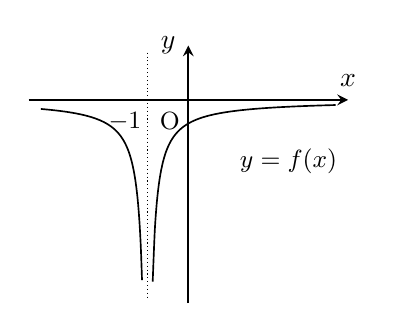
\begin{tikzpicture}[x=0.52cm, y=0.30cm, line width=0.5pt]
  \draw[->, >=stealth, line width=0.7pt] (-3.9,0) -- (3.9,0) node[above=1pt] {$x$};
  \draw[->, >=stealth, line width=0.7pt] (0,-8.6) -- (0,2.3) node[left=1pt] {$y$};
  \draw[densely dotted, line width=0.4pt] (-1,2.0) -- (-1,-8.4);
  \draw[line width=0.6pt, domain=-3.6:-1.13, samples=90, smooth] plot (\x, {-1/(-\x-1)});
  \draw[line width=0.6pt, domain=-0.87:3.6, samples=90, smooth] plot (\x, {-1/(\x+1)});
  \node[below=1pt, font=\small] at (-1.55,0) {$-1$};
  \node[below=1pt, font=\small] at (-0.45,0) {$\pt{O}$};
  \node[right=1pt, font=\small] at (0.95,-2.6) {$y=f(x)$};
\end{tikzpicture}
}\end{minipage}\par
\dmsubprob{1} $\displaystyle\lim_{x\to -1} f(x)$
\dmsubprob{2} $\displaystyle\lim_{x\to\infty} f(x)$
\dmsubprob{3} $\displaystyle\lim_{x\to-\infty} f(x)$
}\vspace{8mm}
\setcounter{dmproblemcount}{16}\dmpnum{10-17}{% id: 10-17
% book: 베이직쎈 미적분1 · 01 함수의 극한
% section: 개념 03 함수의 발산
% passage: 함수 $f(x)$에 대하여 $y=f(x)$의 그래프를 이용하여 다음 극한을 조사하시오.
% figure: tikz:fig-10-17
% answer: 
% answer_source: 
% variant_level: 0 (원본 전사)
% 이 파일은 build.mjs 가 items.json 에서 만든다. 고칠 때는 items.json 을 고친다.
\smash{\raisebox{1.5mm}{\dmkichul{베이직쎈 미적분1 10쪽 17번}}}
\noindent\begin{minipage}[t]{0.58\linewidth}\vspace{0pt}\raggedright $f(x)=x+5$\end{minipage}\hfill\begin{minipage}[t]{0.4\linewidth}\vspace{0pt}\centering \resizebox{\ifdim\width>\linewidth\linewidth\else\width\fi}{!}{% 10-17(10쪽) — f(x)=x+5 의 그래프($x$절편 -5 · $y$절편 5 인 직선). 스캔 화질이 낮아 TikZ 로 다시 그림.
% 원문에 있는 것만: 눈금 -5, 5 · 라벨 O, x, y, y=f(x).
\begin{tikzpicture}[scale=0.40, line width=0.5pt]
  \draw[->, >=stealth, line width=0.7pt] (-6.8,0) -- (2.3,0) node[below=1pt] {$x$};
  \draw[->, >=stealth, line width=0.7pt] (0,-1.7) -- (0,7.2) node[left=1pt] {$y$};
  \node[below left=-2pt and -3pt, font=\small] at (0,0) {$\pt{O}$};
  \draw[line width=0.6pt] (-6.3,-1.3) -- (1.3,6.3);
  \node[left=1pt, font=\small] at (0,5) {$5$};
  \node[below=1pt, font=\small] at (-4.4,0) {$-5$};
  \node[right=1pt, font=\small] at (1.35,6.4) {$y=f(x)$};
\end{tikzpicture}
}\end{minipage}\par
\dmsubprob{1} $\displaystyle\lim_{x\to\infty} f(x)$
\dmsubprob{2} $\displaystyle\lim_{x\to-\infty} f(x)$
}\vspace{8mm}
\dmpassage{다음 극한을 그래프를 이용하여 조사하시오.}
\vspace{3mm}\setcounter{dmproblemcount}{17}\dmpnum{10-18}{% id: 10-18
% book: 베이직쎈 미적분1 · 01 함수의 극한
% section: 개념 03 함수의 발산
% passage: 다음 극한을 그래프를 이용하여 조사하시오.
% figure: none
% answer: 
% answer_source: 
% variant_level: 0 (원본 전사)
% 이 파일은 build.mjs 가 items.json 에서 만든다. 고칠 때는 items.json 을 고친다.
\smash{\raisebox{4.5mm}{\dmkichul{베이직쎈 미적분1 10쪽 18번}}}
$\displaystyle\lim_{x\to 5}\dfrac{1}{|x-5|}$
}\vspace{8mm}
\vspace{3mm}\setcounter{dmproblemcount}{18}\dmpnum{10-19}{% id: 10-19
% book: 베이직쎈 미적분1 · 01 함수의 극한
% section: 개념 03 함수의 발산
% passage: 다음 극한을 그래프를 이용하여 조사하시오.
% figure: none
% answer: 
% answer_source: 
% variant_level: 0 (원본 전사)
% 이 파일은 build.mjs 가 items.json 에서 만든다. 고칠 때는 items.json 을 고친다.
\smash{\raisebox{4.5mm}{\dmkichul{베이직쎈 미적분1 10쪽 19번}}}
$\displaystyle\lim_{x\to 3}\dfrac{1}{(x-3)^2}$
}\vspace{8mm}
\vspace{3mm}\setcounter{dmproblemcount}{19}\dmpnum{10-20}{% id: 10-20
% book: 베이직쎈 미적분1 · 01 함수의 극한
% section: 개념 03 함수의 발산
% passage: 다음 극한을 그래프를 이용하여 조사하시오.
% figure: none
% answer: 
% answer_source: 
% variant_level: 0 (원본 전사)
% 이 파일은 build.mjs 가 items.json 에서 만든다. 고칠 때는 items.json 을 고친다.
\smash{\raisebox{4.5mm}{\dmkichul{베이직쎈 미적분1 10쪽 20번}}}
$\displaystyle\lim_{x\to\infty}(-\sqrt{x})$
}\vspace{8mm}
\vspace{3mm}\setcounter{dmproblemcount}{20}\dmpnum{10-21}{% id: 10-21
% book: 베이직쎈 미적분1 · 01 함수의 극한
% section: 개념 03 함수의 발산
% passage: 다음 극한을 그래프를 이용하여 조사하시오.
% figure: none
% answer: 
% answer_source: 
% variant_level: 0 (원본 전사)
% 이 파일은 build.mjs 가 items.json 에서 만든다. 고칠 때는 items.json 을 고친다.
\smash{\raisebox{4.5mm}{\dmkichul{베이직쎈 미적분1 10쪽 21번}}}
$\displaystyle\lim_{x\to-\infty}(-x^2+2x)$
}\vspace{8mm}
\dmsection{개념 04 우극한과 좌극한}
\dmpassage{함수 $y=f(x)$의 그래프가 오른쪽 그림과 같을 때, 다음 극한값을 구하시오.}
\begin{center}\resizebox{\ifdim\width>\linewidth\linewidth\else\width\fi}{!}{% 11-22(11쪽) — 11-22~11-25 공통. y=f(x) 의 그래프(x=-1 에 빈 점 · x=1 에서 좌·우가 갈리는 그래프). 스캔 화질이 낮아 TikZ 로 다시 그림.
% 원문에 있는 것만: x축 눈금 -2, -1, 1 · y축 눈금 1, -1 · 안내 점선 · 빈 점 (-1,1), (1,-1) · 채운 점 (1,0) · 라벨 y=f(x), O, x, y.
\begin{tikzpicture}[x=0.60cm, y=0.62cm, line width=0.5pt]
  \draw[->, >=stealth, line width=0.7pt] (-3.1,0) -- (3.25,0) node[below=1pt] {$x$};
  \draw[->, >=stealth, line width=0.7pt] (0,-2.2) -- (0,3.2) node[left=1pt] {$y$};
  \node[below left=-2pt and -3pt, font=\small] at (0,0) {$\pt{O}$};
  \draw[densely dotted, line width=0.4pt] (-1,0) -- (-1,1) -- (0,1);
  \draw[densely dotted, line width=0.4pt] (1,0) -- (1,-1) -- (0,-1);
  \draw[line width=0.6pt, domain=-2.45:1, samples=80, smooth] plot (\x, {(\x*\x*\x-4*\x)/3});
  \draw[line width=0.6pt, domain=1:2.8, samples=60, smooth] plot (\x, {0.75*(\x-1)*(\x-1)});
  \fill (1,0) circle (2pt);
  \draw[fill=white, line width=0.5pt] (-1,1) circle (2pt);
  \draw[fill=white, line width=0.5pt] (1,-1) circle (2pt);
  \node[font=\small] at (-2.45,0.38) {$-2$};
  \node[below=1pt, font=\small] at (-1,0) {$-1$};
  \node[below right=-2pt and -3pt, font=\small] at (1,0) {$1$};
  \node[right=1pt, font=\small] at (0,1) {$1$};
  \node[left=1pt, font=\small] at (0,-1) {$-1$};
  \node[font=\small] at (2.1,2.85) {$y=f(x)$};
\end{tikzpicture}
}\end{center}\vspace{4mm}
\vspace{3mm}\setcounter{dmproblemcount}{21}\dmpnum{11-22}{% id: 11-22
% book: 베이직쎈 미적분1 · 01 함수의 극한
% section: 개념 04 우극한과 좌극한
% passage: 함수 $y=f(x)$의 그래프가 오른쪽 그림과 같을 때, 다음 극한값을 구하시오.
% figure: tikz:fig-11-22
% answer: 
% answer_source: 
% variant_level: 0 (원본 전사)
% 이 파일은 build.mjs 가 items.json 에서 만든다. 고칠 때는 items.json 을 고친다.
\smash{\raisebox{4.5mm}{\dmkichul{베이직쎈 미적분1 11쪽 22번}}}
$\displaystyle\lim_{x\to -1+} f(x)$
}\vspace{8mm}
\vspace{3mm}\setcounter{dmproblemcount}{22}\dmpnum{11-23}{% id: 11-23
% book: 베이직쎈 미적분1 · 01 함수의 극한
% section: 개념 04 우극한과 좌극한
% passage: 함수 $y=f(x)$의 그래프가 오른쪽 그림과 같을 때, 다음 극한값을 구하시오.
% figure: tikz:fig-11-22
% answer: 
% answer_source: 
% variant_level: 0 (원본 전사)
% 이 파일은 build.mjs 가 items.json 에서 만든다. 고칠 때는 items.json 을 고친다.
\smash{\raisebox{4.5mm}{\dmkichul{베이직쎈 미적분1 11쪽 23번}}}
$\displaystyle\lim_{x\to -1-} f(x)$
}\vspace{8mm}
\vspace{3mm}\setcounter{dmproblemcount}{23}\dmpnum{11-24}{% id: 11-24
% book: 베이직쎈 미적분1 · 01 함수의 극한
% section: 개념 04 우극한과 좌극한
% passage: 함수 $y=f(x)$의 그래프가 오른쪽 그림과 같을 때, 다음 극한값을 구하시오.
% figure: tikz:fig-11-22
% answer: 
% answer_source: 
% variant_level: 0 (원본 전사)
% 이 파일은 build.mjs 가 items.json 에서 만든다. 고칠 때는 items.json 을 고친다.
\smash{\raisebox{4.5mm}{\dmkichul{베이직쎈 미적분1 11쪽 24번}}}
$\displaystyle\lim_{x\to 1+} f(x)$
}\vspace{8mm}
\vspace{3mm}\setcounter{dmproblemcount}{24}\dmpnum{11-25}{% id: 11-25
% book: 베이직쎈 미적분1 · 01 함수의 극한
% section: 개념 04 우극한과 좌극한
% passage: 함수 $y=f(x)$의 그래프가 오른쪽 그림과 같을 때, 다음 극한값을 구하시오.
% figure: tikz:fig-11-22
% answer: 
% answer_source: 
% variant_level: 0 (원본 전사)
% 이 파일은 build.mjs 가 items.json 에서 만든다. 고칠 때는 items.json 을 고친다.
\smash{\raisebox{4.5mm}{\dmkichul{베이직쎈 미적분1 11쪽 25번}}}
$\displaystyle\lim_{x\to 1-} f(x)$
}\vspace{8mm}
\dmpassage{함수 $y=f(x)$의 그래프가 오른쪽 그림과 같을 때, 다음 극한값을 구하시오.}
\begin{center}\resizebox{\ifdim\width>\linewidth\linewidth\else\width\fi}{!}{% 11-26(11쪽) — 11-26~11-29 공통. y=f(x) 의 그래프(x<2 에서 y=3 · 2<x<=4 에서 오르는 선분 · x>4 에서 가파른 반직선 · x=2 에서 따로 찍힌 점). 스캔 화질이 낮아 TikZ 로 다시 그림.
% 원문에 있는 것만: y축 눈금 1, 2, 3, 5 · x축 눈금 2, 4 · 안내 점선 · 빈 점 (2,3), (2,1), (4,3) · 채운 점 (2,5), (4,2) · 라벨 y=f(x), O, x, y.
\begin{tikzpicture}[x=0.45cm, y=0.47cm, line width=0.5pt]
  \draw[->, >=stealth, line width=0.7pt] (-2.2,0) -- (6.0,0) node[below=1pt] {$x$};
  \draw[->, >=stealth, line width=0.7pt] (0,-1.2) -- (0,6.7) node[left=1pt] {$y$};
  \node[below left=-2pt and -3pt, font=\small] at (0,0) {$\pt{O}$};
  \draw[densely dotted, line width=0.4pt] (0,5) -- (2,5);
  \draw[densely dotted, line width=0.4pt] (2,5) -- (2,0);
  \draw[densely dotted, line width=0.4pt] (2,3) -- (4,3);
  \draw[densely dotted, line width=0.4pt] (0,2) -- (4,2);
  \draw[densely dotted, line width=0.4pt] (0,1) -- (2,1);
  \draw[densely dotted, line width=0.4pt] (4,3) -- (4,0);
  \draw[line width=0.6pt] (-2.1,3) -- (2,3);
  \draw[line width=0.6pt] (2,1) -- (4,2);
  \draw[line width=0.6pt] (4,3) -- (5.8,6.0);
  \fill (2,5) circle (2pt);
  \fill (4,2) circle (2pt);
  \draw[fill=white, line width=0.5pt] (2,3) circle (2pt);
  \draw[fill=white, line width=0.5pt] (2,1) circle (2pt);
  \draw[fill=white, line width=0.5pt] (4,3) circle (2pt);
  \node[left=1pt, font=\small] at (0,5) {$5$};
  \node[left=1pt, font=\small] at (0,3.45) {$3$};
  \node[left=1pt, font=\small] at (0,2) {$2$};
  \node[left=1pt, font=\small] at (0,1) {$1$};
  \node[below=1pt, font=\small] at (2,0) {$2$};
  \node[below=1pt, font=\small] at (4,0) {$4$};
  \node[font=\small] at (3.9,5.95) {$y=f(x)$};
\end{tikzpicture}
}\end{center}\vspace{4mm}
\vspace{3mm}\setcounter{dmproblemcount}{25}\dmpnum{11-26}{% id: 11-26
% book: 베이직쎈 미적분1 · 01 함수의 극한
% section: 개념 04 우극한과 좌극한
% passage: 함수 $y=f(x)$의 그래프가 오른쪽 그림과 같을 때, 다음 극한값을 구하시오.
% figure: tikz:fig-11-26
% answer: 
% answer_source: 
% variant_level: 0 (원본 전사)
% 이 파일은 build.mjs 가 items.json 에서 만든다. 고칠 때는 items.json 을 고친다.
\smash{\raisebox{4.5mm}{\dmkichul{베이직쎈 미적분1 11쪽 26번}}}
$\displaystyle\lim_{x\to 2+} f(x)$
}\vspace{8mm}
\vspace{3mm}\setcounter{dmproblemcount}{26}\dmpnum{11-27}{% id: 11-27
% book: 베이직쎈 미적분1 · 01 함수의 극한
% section: 개념 04 우극한과 좌극한
% passage: 함수 $y=f(x)$의 그래프가 오른쪽 그림과 같을 때, 다음 극한값을 구하시오.
% figure: tikz:fig-11-26
% answer: 
% answer_source: 
% variant_level: 0 (원본 전사)
% 이 파일은 build.mjs 가 items.json 에서 만든다. 고칠 때는 items.json 을 고친다.
\smash{\raisebox{4.5mm}{\dmkichul{베이직쎈 미적분1 11쪽 27번}}}
$\displaystyle\lim_{x\to 2-} f(x)$
}\vspace{8mm}
\vspace{3mm}\setcounter{dmproblemcount}{27}\dmpnum{11-28}{% id: 11-28
% book: 베이직쎈 미적분1 · 01 함수의 극한
% section: 개념 04 우극한과 좌극한
% passage: 함수 $y=f(x)$의 그래프가 오른쪽 그림과 같을 때, 다음 극한값을 구하시오.
% figure: tikz:fig-11-26
% answer: 
% answer_source: 
% variant_level: 0 (원본 전사)
% 이 파일은 build.mjs 가 items.json 에서 만든다. 고칠 때는 items.json 을 고친다.
\smash{\raisebox{4.5mm}{\dmkichul{베이직쎈 미적분1 11쪽 28번}}}
$\displaystyle\lim_{x\to 4+} f(x)$
}\vspace{8mm}
\vspace{3mm}\setcounter{dmproblemcount}{28}\dmpnum{11-29}{% id: 11-29
% book: 베이직쎈 미적분1 · 01 함수의 극한
% section: 개념 04 우극한과 좌극한
% passage: 함수 $y=f(x)$의 그래프가 오른쪽 그림과 같을 때, 다음 극한값을 구하시오.
% figure: tikz:fig-11-26
% answer: 
% answer_source: 
% variant_level: 0 (원본 전사)
% 이 파일은 build.mjs 가 items.json 에서 만든다. 고칠 때는 items.json 을 고친다.
\smash{\raisebox{4.5mm}{\dmkichul{베이직쎈 미적분1 11쪽 29번}}}
$\displaystyle\lim_{x\to 4-} f(x)$
}\vspace{8mm}
\dmpassage{함수 $f(x)=\begin{cases} x+3 & (x\ge 0) \\ -x-3 & (x<0) \end{cases}$의 그래프를 이용하여 다음 극한값을 구하시오.}
\vspace{3mm}\setcounter{dmproblemcount}{29}\dmpnum{11-30}{% id: 11-30
% book: 베이직쎈 미적분1 · 01 함수의 극한
% section: 개념 04 우극한과 좌극한
% passage: 함수 $f(x)=\begin{cases} x+3 & (x\ge 0) \\ -x-3 & (x<0) \end{cases}$의 그래프를 이용하여 다음 극한값을 구하시오.
% figure: none
% answer: 
% answer_source: 
% variant_level: 0 (원본 전사)
% 이 파일은 build.mjs 가 items.json 에서 만든다. 고칠 때는 items.json 을 고친다.
\smash{\raisebox{4.5mm}{\dmkichul{베이직쎈 미적분1 11쪽 30번}}}
$\displaystyle\lim_{x\to 0+} f(x)$
}\vspace{8mm}
\vspace{3mm}\setcounter{dmproblemcount}{30}\dmpnum{11-31}{% id: 11-31
% book: 베이직쎈 미적분1 · 01 함수의 극한
% section: 개념 04 우극한과 좌극한
% passage: 함수 $f(x)=\begin{cases} x+3 & (x\ge 0) \\ -x-3 & (x<0) \end{cases}$의 그래프를 이용하여 다음 극한값을 구하시오.
% figure: none
% answer: 
% answer_source: 
% variant_level: 0 (원본 전사)
% 이 파일은 build.mjs 가 items.json 에서 만든다. 고칠 때는 items.json 을 고친다.
\smash{\raisebox{4.5mm}{\dmkichul{베이직쎈 미적분1 11쪽 31번}}}
$\displaystyle\lim_{x\to 0-} f(x)$
}\vspace{8mm}
\dmpassage{함수 $f(x)=\begin{cases} 2x-1 & (x\ge -1) \\ 2 & (x<-1) \end{cases}$의 그래프를 이용하여 다음 극한값을 구하시오.}
\vspace{3mm}\setcounter{dmproblemcount}{31}\dmpnum{11-32}{% id: 11-32
% book: 베이직쎈 미적분1 · 01 함수의 극한
% section: 개념 04 우극한과 좌극한
% passage: 함수 $f(x)=\begin{cases} 2x-1 & (x\ge -1) \\ 2 & (x<-1) \end{cases}$의 그래프를 이용하여 다음 극한값을 구하시오.
% figure: none
% answer: 
% answer_source: 
% variant_level: 0 (원본 전사)
% 이 파일은 build.mjs 가 items.json 에서 만든다. 고칠 때는 items.json 을 고친다.
\smash{\raisebox{4.5mm}{\dmkichul{베이직쎈 미적분1 11쪽 32번}}}
$\displaystyle\lim_{x\to -1+} f(x)$
}\vspace{8mm}
\vspace{3mm}\setcounter{dmproblemcount}{32}\dmpnum{11-33}{% id: 11-33
% book: 베이직쎈 미적분1 · 01 함수의 극한
% section: 개념 04 우극한과 좌극한
% passage: 함수 $f(x)=\begin{cases} 2x-1 & (x\ge -1) \\ 2 & (x<-1) \end{cases}$의 그래프를 이용하여 다음 극한값을 구하시오.
% figure: none
% answer: 
% answer_source: 
% variant_level: 0 (원본 전사)
% 이 파일은 build.mjs 가 items.json 에서 만든다. 고칠 때는 items.json 을 고친다.
\smash{\raisebox{4.5mm}{\dmkichul{베이직쎈 미적분1 11쪽 33번}}}
$\displaystyle\lim_{x\to -1-} f(x)$
}\vspace{8mm}
\dmsection{개념 05 함수의 극한값의 존재}
\dmpassage{함수 $y=f(x)$의 그래프가 오른쪽 그림과 같을 때, 다음 극한을 조사하시오.}
\begin{center}\resizebox{\ifdim\width>\linewidth\linewidth\else\width\fi}{!}{% 12-34(12쪽) — 34~39번 공통 그림 · y=f(x) 의 그래프(x=-1, x=1 에서 빈 점·채운 점 · 안내 점선). 스캔 화질이 낮아 TikZ 로 다시 그림.
% 원문에 있는 것만: 눈금 -1, 1, 2 · y축 옆 1, -1 · 점선 네 줄 · 빈 점 (-1,1), (1,1), (-1,-1) · 채운 점 (-1,0), (1,0) · 라벨 y=f(x), O, x, y.
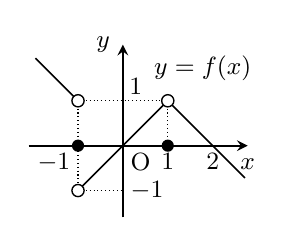
\begin{tikzpicture}[x=0.57cm, y=0.57cm, line width=0.6pt]
  \draw[->, >=stealth, line width=0.7pt] (-2.1,0) -- (2.78,0) node[below=1pt, font=\small] {$x$};
  \draw[->, >=stealth, line width=0.7pt] (0,-1.6) -- (0,2.25) node[left=1pt, font=\small] {$y$};
  \draw[densely dotted, line width=0.4pt] (-1,1) -- (1,1);
  \draw[densely dotted, line width=0.4pt] (-1,1) -- (-1,-1);
  \draw[densely dotted, line width=0.4pt] (1,1) -- (1,0);
  \draw[densely dotted, line width=0.4pt] (-1,-1) -- (0,-1);
  \draw[line width=0.6pt] (-1.95,1.95) -- (-1,1);
  \draw[line width=0.6pt] (-1,-1) -- (1,1);
  \draw[line width=0.6pt] (1,1) -- (2.72,-0.72);
  \draw[fill=white, line width=0.5pt] (-1,1) circle (2.2pt);
  \draw[fill=white, line width=0.5pt] (1,1) circle (2.2pt);
  \draw[fill=white, line width=0.5pt] (-1,-1) circle (2.2pt);
  \fill (-1,0) circle (2.2pt);
  \fill (1,0) circle (2.2pt);
  \node[font=\small, inner sep=2.5pt, below left] at (-1,0) {$-1$};
  \node[font=\small, inner sep=2.5pt, below] at (1,0) {$1$};
  \node[font=\small, inner sep=2.5pt, below] at (2,0) {$2$};
  \node[font=\small, inner sep=2.5pt, below right] at (0,0) {$\pt{O}$};
  \node[font=\small, inner sep=2pt, above right] at (0,1) {$1$};
  \node[font=\small, inner sep=2.5pt, right] at (0,-1) {$-1$};
  \node[font=\small, inner sep=1pt] at (1.78,1.72) {$y=f(x)$};
\end{tikzpicture}
}\end{center}\vspace{4mm}
\vspace{3mm}\setcounter{dmproblemcount}{33}\dmpnum{12-34}{% id: 12-34
% book: 베이직쎈 미적분1 · 01 함수의 극한
% section: 개념 05 함수의 극한값의 존재
% passage: 함수 $y=f(x)$의 그래프가 오른쪽 그림과 같을 때, 다음 극한을 조사하시오.
% figure: tikz:fig-12-34
% answer: 
% answer_source: 
% variant_level: 0 (원본 전사)
% 이 파일은 build.mjs 가 items.json 에서 만든다. 고칠 때는 items.json 을 고친다.
\smash{\raisebox{4.5mm}{\dmkichul{베이직쎈 미적분1 12쪽 34번}}}
$\displaystyle\lim_{x\to 1+} f(x)$
}\vspace{8mm}
\vspace{3mm}\setcounter{dmproblemcount}{34}\dmpnum{12-35}{% id: 12-35
% book: 베이직쎈 미적분1 · 01 함수의 극한
% section: 개념 05 함수의 극한값의 존재
% passage: 함수 $y=f(x)$의 그래프가 오른쪽 그림과 같을 때, 다음 극한을 조사하시오.
% figure: tikz:fig-12-34
% answer: 
% answer_source: 
% variant_level: 0 (원본 전사)
% 이 파일은 build.mjs 가 items.json 에서 만든다. 고칠 때는 items.json 을 고친다.
\smash{\raisebox{4.5mm}{\dmkichul{베이직쎈 미적분1 12쪽 35번}}}
$\displaystyle\lim_{x\to 1-} f(x)$
}\vspace{8mm}
\vspace{3mm}\setcounter{dmproblemcount}{35}\dmpnum{12-36}{% id: 12-36
% book: 베이직쎈 미적분1 · 01 함수의 극한
% section: 개념 05 함수의 극한값의 존재
% passage: 함수 $y=f(x)$의 그래프가 오른쪽 그림과 같을 때, 다음 극한을 조사하시오.
% figure: tikz:fig-12-34
% answer: 
% answer_source: 
% variant_level: 0 (원본 전사)
% 이 파일은 build.mjs 가 items.json 에서 만든다. 고칠 때는 items.json 을 고친다.
\smash{\raisebox{4.5mm}{\dmkichul{베이직쎈 미적분1 12쪽 36번}}}
$\displaystyle\lim_{x\to 1} f(x)$
}\vspace{8mm}
\vspace{3mm}\setcounter{dmproblemcount}{36}\dmpnum{12-37}{% id: 12-37
% book: 베이직쎈 미적분1 · 01 함수의 극한
% section: 개념 05 함수의 극한값의 존재
% passage: 함수 $y=f(x)$의 그래프가 오른쪽 그림과 같을 때, 다음 극한을 조사하시오.
% figure: tikz:fig-12-34
% answer: 
% answer_source: 
% variant_level: 0 (원본 전사)
% 이 파일은 build.mjs 가 items.json 에서 만든다. 고칠 때는 items.json 을 고친다.
\smash{\raisebox{4.5mm}{\dmkichul{베이직쎈 미적분1 12쪽 37번}}}
$\displaystyle\lim_{x\to -1+} f(x)$
}\vspace{8mm}
\vspace{3mm}\setcounter{dmproblemcount}{37}\dmpnum{12-38}{% id: 12-38
% book: 베이직쎈 미적분1 · 01 함수의 극한
% section: 개념 05 함수의 극한값의 존재
% passage: 함수 $y=f(x)$의 그래프가 오른쪽 그림과 같을 때, 다음 극한을 조사하시오.
% figure: tikz:fig-12-34
% answer: 
% answer_source: 
% variant_level: 0 (원본 전사)
% 이 파일은 build.mjs 가 items.json 에서 만든다. 고칠 때는 items.json 을 고친다.
\smash{\raisebox{4.5mm}{\dmkichul{베이직쎈 미적분1 12쪽 38번}}}
$\displaystyle\lim_{x\to -1-} f(x)$
}\vspace{8mm}
\vspace{3mm}\setcounter{dmproblemcount}{38}\dmpnum{12-39}{% id: 12-39
% book: 베이직쎈 미적분1 · 01 함수의 극한
% section: 개념 05 함수의 극한값의 존재
% passage: 함수 $y=f(x)$의 그래프가 오른쪽 그림과 같을 때, 다음 극한을 조사하시오.
% figure: tikz:fig-12-34
% answer: 
% answer_source: 
% variant_level: 0 (원본 전사)
% 이 파일은 build.mjs 가 items.json 에서 만든다. 고칠 때는 items.json 을 고친다.
\smash{\raisebox{4.5mm}{\dmkichul{베이직쎈 미적분1 12쪽 39번}}}
$\displaystyle\lim_{x\to -1} f(x)$
}\vspace{8mm}
\dmpassage{함수 $f(x)=\begin{cases} -x+4 & (x\ge -4) \\ \dfrac{1}{2}x+2 & (x<-4) \end{cases}$의 그래프를 이용하여 다음 극한을 조사하시오.}
\vspace{3mm}\setcounter{dmproblemcount}{39}\dmpnum{12-40}{% id: 12-40
% book: 베이직쎈 미적분1 · 01 함수의 극한
% section: 개념 05 함수의 극한값의 존재
% passage: 함수 $f(x)=\begin{cases} -x+4 & (x\ge -4) \\ \dfrac{1}{2}x+2 & (x<-4) \end{cases}$의 그래프를 이용하여 다음 극한을 조사하시오.
% figure: none
% answer: 
% answer_source: 
% variant_level: 0 (원본 전사)
% 이 파일은 build.mjs 가 items.json 에서 만든다. 고칠 때는 items.json 을 고친다.
\smash{\raisebox{4.5mm}{\dmkichul{베이직쎈 미적분1 12쪽 40번}}}
$\displaystyle\lim_{x\to -4+} f(x)$
}\vspace{8mm}
\vspace{3mm}\setcounter{dmproblemcount}{40}\dmpnum{12-41}{% id: 12-41
% book: 베이직쎈 미적분1 · 01 함수의 극한
% section: 개념 05 함수의 극한값의 존재
% passage: 함수 $f(x)=\begin{cases} -x+4 & (x\ge -4) \\ \dfrac{1}{2}x+2 & (x<-4) \end{cases}$의 그래프를 이용하여 다음 극한을 조사하시오.
% figure: none
% answer: 
% answer_source: 
% variant_level: 0 (원본 전사)
% 이 파일은 build.mjs 가 items.json 에서 만든다. 고칠 때는 items.json 을 고친다.
\smash{\raisebox{4.5mm}{\dmkichul{베이직쎈 미적분1 12쪽 41번}}}
$\displaystyle\lim_{x\to -4-} f(x)$
}\vspace{8mm}
\vspace{3mm}\setcounter{dmproblemcount}{41}\dmpnum{12-42}{% id: 12-42
% book: 베이직쎈 미적분1 · 01 함수의 극한
% section: 개념 05 함수의 극한값의 존재
% passage: 함수 $f(x)=\begin{cases} -x+4 & (x\ge -4) \\ \dfrac{1}{2}x+2 & (x<-4) \end{cases}$의 그래프를 이용하여 다음 극한을 조사하시오.
% figure: none
% answer: 
% answer_source: 
% variant_level: 0 (원본 전사)
% 이 파일은 build.mjs 가 items.json 에서 만든다. 고칠 때는 items.json 을 고친다.
\smash{\raisebox{4.5mm}{\dmkichul{베이직쎈 미적분1 12쪽 42번}}}
$\displaystyle\lim_{x\to -4} f(x)$
}\vspace{8mm}
\dmpassage{다음 극한을 조사하시오.}
\vspace{3mm}\setcounter{dmproblemcount}{42}\dmpnum{12-43}{% id: 12-43
% book: 베이직쎈 미적분1 · 01 함수의 극한
% section: 개념 05 함수의 극한값의 존재
% passage: 다음 극한을 조사하시오.
% figure: tikz:fig-12-43
% answer: 
% answer_source: 
% variant_level: 0 (원본 전사)
% 이 파일은 build.mjs 가 items.json 에서 만든다. 고칠 때는 items.json 을 고친다.
\smash{\raisebox{4.5mm}{\dmkichul{베이직쎈 미적분1 12쪽 43번}}}
\noindent\begin{minipage}[t]{0.58\linewidth}\vspace{0pt}\raggedright $\displaystyle\lim_{x\to 0}\dfrac{|x|}{x}$\end{minipage}\hfill\begin{minipage}[t]{0.4\linewidth}\vspace{0pt}\centering \resizebox{\ifdim\width>\linewidth\linewidth\else\width\fi}{!}{% 12-43(12쪽) — 43번 풀이 힌트의 그림 · y=|x|/x 의 그래프(x>0 에서 y=1, x<0 에서 y=-1 · 원점에서 끊긴 빈 점 · 다가가는 방향 화살표 네 개). 스캔 화질이 낮아 TikZ 로 다시 그림.
% 원문에 있는 것만: 빈 점 (0,1), (0,-1) · 라벨 1, -1, y=f(x), O, x, y · 접근 화살표. 눈금은 만들지 않는다.
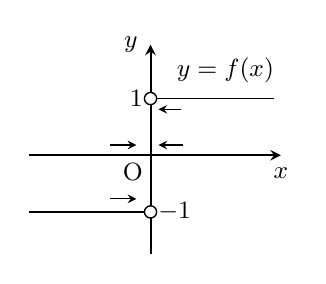
\begin{tikzpicture}[x=0.72cm, y=0.72cm, line width=0.6pt]
  \draw[->, >=stealth, line width=0.7pt] (-2.15,0) -- (2.3,0) node[below=1pt, font=\small] {$x$};
  \draw[->, >=stealth, line width=0.7pt] (0,-1.75) -- (0,1.95) node[left=1pt, font=\small] {$y$};
  \draw[line width=0.6pt] (0,1) -- (2.18,1);
  \draw[line width=0.6pt] (-2.14,-1) -- (0,-1);
  \draw[fill=white, line width=0.5pt] (0,1) circle (2.2pt);
  \draw[fill=white, line width=0.5pt] (0,-1) circle (2.2pt);
  \draw[->, >=stealth, line width=0.4pt] (0.54,0.81) -- (0.14,0.81);
  \draw[->, >=stealth, line width=0.4pt] (-0.71,-0.77) -- (-0.25,-0.77);
  \draw[->, >=stealth, line width=0.4pt] (-0.71,0.18) -- (-0.25,0.18);
  \draw[->, >=stealth, line width=0.4pt] (0.57,0.18) -- (0.14,0.18);
  \node[font=\small, inner sep=2.5pt, left] at (0,1) {$1$};
  \node[font=\small, inner sep=2.5pt, right] at (0,-1) {$-1$};
  \node[font=\small, inner sep=2.5pt, below left] at (0,0) {$\pt{O}$};
  \node[font=\small, inner sep=1pt] at (1.32,1.5) {$y=f(x)$};
\end{tikzpicture}
}\end{minipage}\par
\dmhint{$|x|=\begin{cases} x & (x\ge 0) \\ -x & (x<0) \end{cases}$이므로 $f(x)=\dfrac{|x|}{x}$로 놓으면\hfill{\footnotesize $f(x)$는 $x=0$에서 정의되지 않는다.}\\ $f(x)=\begin{cases} \blank & (x>0) \\ \blank & (x<0) \end{cases}$\\ $y=f(x)$의 그래프는 오른쪽 그림과 같으므로\\ $\displaystyle\lim_{x\to 0+} f(x)=\blank$,\\ $\displaystyle\lim_{x\to 0-} f(x)=\blank$\\ 따라서 $\displaystyle\lim_{x\to 0+} f(x)\ne\lim_{x\to 0-} f(x)$이므로\\ $\displaystyle\lim_{x\to 0} f(x)$, 즉 $\displaystyle\lim_{x\to 0}\dfrac{|x|}{x}$의 값은 \blank[6em].}
}\vspace{8mm}
\vspace{3mm}\setcounter{dmproblemcount}{43}\dmpnum{12-44}{% id: 12-44
% book: 베이직쎈 미적분1 · 01 함수의 극한
% section: 개념 05 함수의 극한값의 존재
% passage: 다음 극한을 조사하시오.
% figure: none
% answer: 
% answer_source: 
% variant_level: 0 (원본 전사)
% 이 파일은 build.mjs 가 items.json 에서 만든다. 고칠 때는 items.json 을 고친다.
\smash{\raisebox{4.5mm}{\dmkichul{베이직쎈 미적분1 12쪽 44번}}}
$\displaystyle\lim_{x\to 2}\dfrac{|2-x|}{x-2}$
}\vspace{8mm}
\vspace{3mm}\setcounter{dmproblemcount}{44}\dmpnum{12-45}{% id: 12-45
% book: 베이직쎈 미적분1 · 01 함수의 극한
% section: 개념 05 함수의 극한값의 존재
% passage: 다음 극한을 조사하시오.
% figure: none
% answer: 
% answer_source: 
% variant_level: 0 (원본 전사)
% 이 파일은 build.mjs 가 items.json 에서 만든다. 고칠 때는 items.json 을 고친다.
\smash{\raisebox{4.5mm}{\dmkichul{베이직쎈 미적분1 12쪽 45번}}}
$\displaystyle\lim_{x\to 0}\dfrac{x^2}{|x|}$
}\vspace{8mm}
\dmsection{유형 001 함수의 수렴과 발산}
\setcounter{dmproblemcount}{0}\dmpnum{13-01}{% id: 13-01
% book: 베이직쎈 미적분1 · 01 함수의 극한
% section: 유형 001 함수의 수렴과 발산
% figure: none
% answer: 
% answer_source: 
% variant_level: 0 (원본 전사)
% 이 파일은 build.mjs 가 items.json 에서 만든다. 고칠 때는 items.json 을 고친다.
\smash{\raisebox{1.5mm}{\dmkichul{베이직쎈 미적분1 13쪽 01번}}}
$x\to 0$일 때, 함수 $f(x)$가 수렴하는 것만을 \textbf{보기}에서 있는 대로 고른 것은? \bogi{\begin{minipage}[t]{0.48\linewidth}\raggedright ㄱ.\hspace{1.5mm}% 13-01(13쪽) — 보기 ㄱ 의 그래프(원점을 지나 오른쪽 아래로 내려가는 직선). 스캔 화질이 낮아 TikZ 로 다시 그림.
% 원문에 있는 것만: 직선 하나 · 라벨 O, x, y, y=f(x). 눈금·좌표값은 원문에 없으므로 넣지 않는다.
\begin{tikzpicture}[baseline=(current bounding box.north), x=0.38cm, y=0.38cm, line width=0.55pt]
  \draw[->, >=stealth, line width=0.7pt] (-2.5,0) -- (2.6,0) node[below=1pt] {$x$};
  \draw[->, >=stealth, line width=0.7pt] (0,-2.5) -- (0,2.4) node[left=1pt] {$y$};
  \node[below left=-2pt and -3pt, font=\small] at (0,0) {$\pt{O}$};
  \draw (-1.95,1.95) -- (2.05,-1.85);
  \node[anchor=west, font=\small] at (0.2,-2.2) {$y=f(x)$};
\end{tikzpicture}
\end{minipage}\begin{minipage}[t]{0.48\linewidth}\raggedright ㄴ.\hspace{1.5mm}% 13-01(13쪽) — 보기 ㄴ 의 그래프(꼭짓점이 $(0,\,-2)$ 인 V 자 그래프). 스캔 화질이 낮아 TikZ 로 다시 그림.
% 원문에 있는 것만: y축 눈금 -2 · 두 반직선 · 라벨 O, x, y, y=f(x).
\begin{tikzpicture}[baseline=(current bounding box.north), x=0.38cm, y=0.38cm, line width=0.55pt]
  \draw[->, >=stealth, line width=0.7pt] (-2.55,0) -- (2.5,0) node[below=1pt] {$x$};
  \draw[->, >=stealth, line width=0.7pt] (0,-2.4) -- (0,2.6) node[left=1pt] {$y$};
  \draw (-1.5,1.75) -- (0,-2) -- (1.55,1.9);
  \node[above left=-3pt and -3pt, font=\small] at (0,0) {$\pt{O}$};
  \node[left=2pt, font=\small] at (0,-2) {$-2$};
  \node[anchor=west, font=\small] at (0.45,2.35) {$y=f(x)$};
\end{tikzpicture}
\end{minipage}\par\medskip\begin{minipage}[t]{0.48\linewidth}\raggedright ㄷ.\hspace{1.5mm}% 13-01(13쪽) — 보기 ㄷ 의 그래프(x축·y축을 점근선으로 하는 두 갈래 곡선 · 왼쪽 갈래는 x축 위, 오른쪽 갈래는 x축 아래).
% 스캔 화질이 낮아 TikZ 로 다시 그림. 원문에 있는 것만: 두 갈래 곡선 · 라벨 O, x, y, y=f(x)(눈금 없음).
\begin{tikzpicture}[baseline=(current bounding box.north), x=0.38cm, y=0.38cm, line width=0.55pt]
  \draw[->, >=stealth, line width=0.7pt] (-2.75,0) -- (2.65,0);
  \draw[->, >=stealth, line width=0.7pt] (0,-2.9) -- (0,2.65) node[right=1pt] {$y$};
  \draw[line width=0.6pt, domain=-2.7:-0.21, samples=80, smooth] plot (\x, {-0.5/\x});
  \draw[line width=0.6pt, domain=0.21:2.7, samples=80, smooth] plot (\x, {-0.5/\x});
  \node[above=1pt, font=\small] at (2.25,0) {$x$};
  \node[below left=-3pt and -3pt, font=\small] at (0,0) {$\pt{O}$};
  \node[anchor=west, font=\small] at (0.25,-2.3) {$y=f(x)$};
\end{tikzpicture}
\end{minipage}\begin{minipage}[t]{0.48\linewidth}\raggedright ㄹ.\hspace{1.5mm}% 13-01(13쪽) — 보기 ㄹ 의 그래프(원점에서 채운 점으로 끊기고 $(0,\,1)$ 의 빈 점에서 다시 시작하는 두 반직선).
% 스캔 화질이 낮아 TikZ 로 다시 그림. 원문의 빈 점(○)·채운 점(●) 과 y축 눈금 1 을 그대로 옮긴다.
\begin{tikzpicture}[baseline=(current bounding box.north), x=0.28cm, y=0.28cm, line width=0.55pt]
  \draw[->, >=stealth, line width=0.7pt] (-3.4,0) -- (3.3,0) node[below=1pt] {$x$};
  \draw[->, >=stealth, line width=0.7pt] (0,-2.75) -- (0,3.75) node[left=1pt] {$y$};
  \draw (-2.9,-2.4) -- (0,0);
  \draw (0,1) -- (2.4,3.0);
  \fill (0,0) circle (2.2pt);
  \draw[fill=white] (0,1) circle (2.2pt);
  \node[left=1pt, font=\small] at (0,1) {$1$};
  \node[below right=-2pt and -2pt, font=\small] at (0,0) {$\pt{O}$};
  \node[anchor=west, font=\small] at (0.5,3.6) {$y=f(x)$};
\end{tikzpicture}
\end{minipage}}
\dmchoicesauto{}{ㄱ, ㄴ}{ㄱ, ㄷ}{ㄴ, ㄹ}{ㄱ, ㄴ, ㄷ}{ㄱ, ㄴ, ㄹ}
}\vspace{8mm}
\setcounter{dmproblemcount}{1}\dmpnum{13-02}{% id: 13-02
% book: 베이직쎈 미적분1 · 01 함수의 극한
% section: 유형 001 함수의 수렴과 발산
% figure: none
% answer: 
% answer_source: 
% variant_level: 0 (원본 전사)
% 이 파일은 build.mjs 가 items.json 에서 만든다. 고칠 때는 items.json 을 고친다.
\smash{\raisebox{1.5mm}{\dmkichul{베이직쎈 미적분1 13쪽 02번}}}
$x$의 값이 한없이 커질 때, 함수 $f(x)$가 수렴하는 것만을 \textbf{보기}에서 있는 대로 고른 것은? \bogi{\begin{minipage}{0.96\linewidth}\raggedright ㄱ. $f(x)=\dfrac{1}{5x}$ \qquad ㄴ. $f(x)=x^2-1$\\[1mm] ㄷ. $f(x)=\dfrac{x}{x+1}$ \qquad ㄹ. $f(x)=\sqrt{6}$\end{minipage}}
\dmchoicesauto{}{ㄱ, ㄴ}{ㄱ, ㄹ}{ㄴ, ㄹ}{ㄱ, ㄷ, ㄹ}{ㄴ, ㄷ, ㄹ}
}\vspace{8mm}
\setcounter{dmproblemcount}{2}\dmpnum{13-03}{% id: 13-03
% book: 베이직쎈 미적분1 · 01 함수의 극한
% section: 유형 001 함수의 수렴과 발산
% figure: none
% answer: 
% answer_source: 
% variant_level: 0 (원본 전사)
% 이 파일은 build.mjs 가 items.json 에서 만든다. 고칠 때는 items.json 을 고친다.
\smash{\raisebox{1.5mm}{\dmkichul{베이직쎈 미적분1 13쪽 03번}}}
다음 중 옳지 \underline{않은} 것은?
\begin{choicesii}{\rule[-3ex]{0pt}{8ex}$\displaystyle\lim_{x\to\infty}\left(-\dfrac{2}{x}\right)=0$}{\rule[-3ex]{0pt}{8ex}$\displaystyle\lim_{x\to\infty}\sqrt{x-7}=\infty$}{\rule[-3ex]{0pt}{8ex}$\displaystyle\lim_{x\to\infty}\left(\dfrac{1}{x^2}-1\right)=-1$}{\rule[-3ex]{0pt}{8ex}$\displaystyle\lim_{x\to-\infty}(x^2+4)=\infty$}{\rule[-3ex]{0pt}{8ex}$\displaystyle\lim_{x\to-\infty}\dfrac{3}{x-1}=-\infty$}\end{choicesii}
}\vspace{8mm}
\dmsection{유형 002 우극한과 좌극한}
\vspace{3mm}\setcounter{dmproblemcount}{3}\dmpnum{13-04}{% id: 13-04
% book: 베이직쎈 미적분1 · 01 함수의 극한
% section: 유형 002 우극한과 좌극한
% figure: tikz:fig-13-04
% answer: 
% answer_source: 
% variant_level: 0 (원본 전사)
% 이 파일은 build.mjs 가 items.json 에서 만든다. 고칠 때는 items.json 을 고친다.
\smash{\raisebox{4.5mm}{\dmkichul{베이직쎈 미적분1 13쪽 04번}}}
\noindent\begin{minipage}[t]{0.58\linewidth}\vspace{0pt}\raggedright 함수 $y=f(x)$의 그래프가 오른쪽 그림과 같을 때,\par\smallskip\end{minipage}\hfill\begin{minipage}[t]{0.4\linewidth}\vspace{0pt}\centering \resizebox{\ifdim\width>\linewidth\linewidth\else\width\fi}{!}{% 13-04(13쪽) — y=f(x) 의 그래프(꺾인 선이 (1,0) 에서 올라가 (2,1) 빈 점에서 끊기고 (2,3) 채운 점부터 가로 반직선).
% 스캔 화질이 낮아 TikZ 로 다시 그림. 원문의 빈 점(○)·채운 점(●)·점선·눈금 1, 3, 1, 2 만 옮긴다.
\begin{tikzpicture}[x=0.52cm, y=0.36cm, line width=0.55pt]
  \draw[->, >=stealth, line width=0.7pt] (-2.1,0) -- (3.6,0) node[below=1pt] {$x$};
  \draw[->, >=stealth, line width=0.7pt] (0,-1.1) -- (0,4.3) node[left=1pt] {$y$};
  \draw[densely dashed, line width=0.4pt] (0,3) -- (2,3);
  \draw[densely dashed, line width=0.4pt] (0,1) -- (2,1);
  \draw[densely dashed, line width=0.4pt] (2,3) -- (2,0);
  \draw[line width=0.6pt] (-1.75,2.75) -- (1,0) -- (2,1);
  \draw[line width=0.6pt] (2,3) -- (3.5,3);
  \draw[fill=white] (2,1) circle (2.2pt);
  \fill (2,3) circle (2.2pt);
  \node[left=1pt, font=\small] at (0,1) {$1$};
  \node[left=1pt, font=\small] at (0,3) {$3$};
  \node[below left=-2pt and -4pt, font=\small] at (0,0) {$\pt{O}$};
  \node[below=1pt, font=\small] at (1,0) {$1$};
  \node[below=1pt, font=\small] at (2,0) {$2$};
  \node[anchor=west, font=\small] at (2.15,3.8) {$y=f(x)$};
\end{tikzpicture}
}\end{minipage}\par
\noindent \dispeq{$\displaystyle\lim_{x\to 2+} f(x)+\lim_{x\to 2-} f(x)$}\par\smallskip\noindent 의 값을 구하시오.
}\vspace{8mm}
\vspace{3mm}\setcounter{dmproblemcount}{4}\dmpnum{13-05}{% id: 13-05
% book: 베이직쎈 미적분1 · 01 함수의 극한
% section: 유형 002 우극한과 좌극한
% figure: tikz:fig-13-05
% answer: 
% answer_source: 
% variant_level: 0 (원본 전사)
% 이 파일은 build.mjs 가 items.json 에서 만든다. 고칠 때는 items.json 을 고친다.
\smash{\raisebox{4.5mm}{\dmkichul{베이직쎈 미적분1 13쪽 05번}}}
함수 $y=f(x)$의 그래프가 다음 그림과 같을 때, $\displaystyle\lim_{x\to-1-} f(x)-\lim_{x\to 0+} f(x)+f(1)$의 값을 구하시오.
\par\smallskip\begin{center}\resizebox{\ifdim\width>\linewidth\linewidth\else\width\fi}{!}{% 13-05(13쪽) — y=f(x) 의 그래프(x=-1, x=0, x=1 에서 끊기는 네 조각). 스캔 화질이 낮아 TikZ 로 다시 그림.
% 원문의 빈 점(○)·채운 점(●)·점선과 눈금 1, 1/2, -1/2, -1, 1 만 옮긴다.
\begin{tikzpicture}[x=1.05cm, y=1.05cm, line width=0.55pt]
  \draw[->, >=stealth, line width=0.7pt] (-2.3,0) -- (2.5,0) node[below=1pt] {$x$};
  \draw[->, >=stealth, line width=0.7pt] (0,-1.05) -- (0,1.5) node[left=1pt] {$y$};
  \draw[densely dashed, line width=0.4pt] (-1,1) -- (1,1);
  \draw[densely dashed, line width=0.4pt] (-1,0.5) -- (0,0.5);
  \draw[densely dashed, line width=0.4pt] (-1,0) -- (-1,1);
  \draw[densely dashed, line width=0.4pt] (1,0) -- (1,1);
  \draw[line width=0.6pt] (-2.2,0.5) -- (-1,0.5);
  \draw[line width=0.6pt] (-1,1) -- (0,0);
  \draw[line width=0.6pt, domain=0:1, samples=50, smooth] plot (\x, {0.5*\x*\x-0.5});
  \draw[line width=0.6pt, domain=1:2.3, samples=60, smooth] plot (\x, {1/\x});
  \fill (-1,0.5) circle (2.2pt);
  \draw[fill=white] (-1,1) circle (2.2pt);
  \draw[fill=white] (0,0) circle (2.2pt);
  \fill (0,-0.5) circle (2.2pt);
  \draw[fill=white] (1,0) circle (2.2pt);
  \fill (1,1) circle (2.2pt);
  \node[above left=-1pt and -1pt, font=\small] at (0,1) {$1$};
  \node[right=2pt, font=\small] at (0,0.5) {$\dfrac{1}{2}$};
  \node[left=2pt, font=\small] at (0,-0.5) {$-\dfrac{1}{2}$};
  \node[below=1pt, font=\small] at (-1,0) {$-1$};
  \node[below right=-2pt and -3pt, font=\small] at (0,0) {$\pt{O}$};
  \node[below=1pt, font=\small] at (1,0) {$1$};
  \node[anchor=west, font=\small] at (0.3,1.3) {$y=f(x)$};
\end{tikzpicture}
}\end{center}
}\vspace{8mm}
\setcounter{dmproblemcount}{5}\dmpnum{14-06}{% id: 14-06
% book: 베이직쎈 미적분1 · 01 함수의 극한
% section: 유형 002 우극한과 좌극한
% figure: tikz:fig-14-06
% answer: 
% answer_source: 
% variant_level: 0 (원본 전사)
% 이 파일은 build.mjs 가 items.json 에서 만든다. 고칠 때는 items.json 을 고친다.
\smash{\raisebox{1.5mm}{\dmkichul{베이직쎈 미적분1 14쪽 06번}}}
\noindent\begin{minipage}[t]{0.58\linewidth}\vspace{0pt}\raggedright 함수 $y=f(x)$의 그래프가 오른쪽 그림과 같을 때, 다음 중 옳은 것은?\end{minipage}\hfill\begin{minipage}[t]{0.4\linewidth}\vspace{0pt}\centering \resizebox{\ifdim\width>\linewidth\linewidth\else\width\fi}{!}{% 14-06(14쪽) — y=f(x) 의 그래프(x=-1 과 x=1 에서 끊기는 세 조각). 스캔 화질이 낮아 TikZ 로 다시 그림.
% 원문의 빈 점(○)·채운 점(●)·점선과 눈금 2, 1, -1, -2, -1, 1, 2 만 옮긴다.
\begin{tikzpicture}[x=0.56cm, y=0.56cm, line width=0.55pt]
  \draw[->, >=stealth, line width=0.7pt] (-2.2,0) -- (3.4,0) node[below=1pt] {$x$};
  \draw[->, >=stealth, line width=0.7pt] (0,-3.4) -- (0,2.9) node[left=1pt] {$y$};
  \draw[densely dashed, line width=0.4pt] (0,2) -- (1,2);
  \draw[densely dashed, line width=0.4pt] (0,1) -- (1,1);
  \draw[densely dashed, line width=0.4pt] (1,2) -- (1,0);
  \draw[densely dashed, line width=0.4pt] (-1,-1) -- (0,-1);
  \draw[densely dashed, line width=0.4pt] (-1,-2) -- (0,-2);
  \draw[densely dashed, line width=0.4pt] (-1,0) -- (-1,-2);
  \draw[line width=0.6pt, smooth] plot coordinates {(-1.95,-3.1) (-1.65,-2.62) (-1.35,-2.26) (-1,-2)};
  \draw[line width=0.6pt, smooth] plot coordinates {(-1,-1) (-0.55,0) (-0.1,0.85) (0.35,1.25) (0.7,1.2) (1,1)};
  \draw[line width=0.6pt] (1,2) -- (3.15,-2.3);
  \fill (-1,-2) circle (2.2pt);
  \draw[fill=white] (-1,-1) circle (2.2pt);
  \fill (1,1) circle (2.2pt);
  \draw[fill=white] (1,2) circle (2.2pt);
  \node[left=1pt, font=\small] at (0,2) {$2$};
  \node[left=1pt, font=\small] at (0,1) {$1$};
  \node[right=1pt, font=\small] at (0,-1) {$-1$};
  \node[right=1pt, font=\small] at (0,-2) {$-2$};
  \node[font=\small] at (-1.5,0.42) {$-1$};
  \node[below left=-2pt and -4pt, font=\small] at (0,0) {$\pt{O}$};
  \node[below=1pt, font=\small] at (1,0) {$1$};
  \node[below left=-1pt and -4pt, font=\small] at (2,0) {$2$};
  \node[anchor=west, font=\small] at (0.35,2.6) {$y=f(x)$};
\end{tikzpicture}
}\end{minipage}\par
\begin{choicesv}{$\displaystyle\lim_{x\to-1+} f(x)=0$}{$\displaystyle\lim_{x\to-1-} f(x)=-1$}{$\displaystyle\lim_{x\to 1+} f(x)=2$}{$\displaystyle\lim_{x\to 1-} f(x)=0$}{$\displaystyle\lim_{x\to 2-} f(x)=1$}\end{choicesv}
}\vspace{8mm}
\vspace{3mm}\setcounter{dmproblemcount}{6}\dmpnum{14-07}{% id: 14-07
% book: 베이직쎈 미적분1 · 01 함수의 극한
% section: 유형 002 우극한과 좌극한
% figure: tikz:fig-14-07
% answer: 
% answer_source: 
% variant_level: 0 (원본 전사)
% 이 파일은 build.mjs 가 items.json 에서 만든다. 고칠 때는 items.json 을 고친다.
\smash{\raisebox{4.5mm}{\dmkichul{베이직쎈 미적분1 14쪽 07번}}}
\noindent\begin{minipage}[t]{0.58\linewidth}\vspace{0pt}\raggedright 함수 $y=f(x)$의 그래프가 오른쪽 그림과 같다. $\displaystyle\lim_{x\to-2+} f(x)=5$일 때, 상수 $a$의 값과 $\displaystyle\lim_{x\to-2-} f(x)$의 값을 차례대로 구하시오.\end{minipage}\hfill\begin{minipage}[t]{0.4\linewidth}\vspace{0pt}\centering \resizebox{\ifdim\width>\linewidth\linewidth\else\width\fi}{!}{% 14-07(14쪽) — y=f(x) 의 그래프(x=-2 에서 끊기는 두 조각 · 왼쪽은 y=a-2 인 반직선, 오른쪽은 위로 볼록한 곡선).
% 스캔 화질이 낮아 TikZ 로 다시 그림. 원문의 빈 점(○)·채운 점(●)·점선과 눈금 a+2, a, a-2, -2 만 옮긴다.
\begin{tikzpicture}[x=0.55cm, y=0.55cm, line width=0.55pt]
  \draw[->, >=stealth, line width=0.7pt] (-3.15,0) -- (3.35,0) node[below=1pt] {$x$};
  \draw[->, >=stealth, line width=0.7pt] (0,-1.7) -- (0,3.5) node[left=1pt] {$y$};
  \draw[densely dashed, line width=0.4pt] (-2,1.95) -- (0,1.95);
  \draw[densely dashed, line width=0.4pt] (-2,1.15) -- (0,1.15);
  \draw[densely dashed, line width=0.4pt] (-2,0.35) -- (0,0.35);
  \draw[densely dashed, line width=0.4pt] (-2,1.95) -- (-2,0);
  \draw[line width=0.6pt] (-3.05,0.35) -- (-2,0.35);
  \draw[line width=0.6pt, smooth] plot coordinates {(-2,1.95) (-1.5,2.45) (-1,2.72) (-0.35,2.85) (0.3,2.78) (1.0,2.6) (1.6,2.1) (1.95,1.5) (2.2,0.8) (2.45,0) (2.7,-0.9) (2.85,-1.5)};
  \draw[fill=white] (-2,0.35) circle (2.2pt);
  \fill (-2,1.15) circle (2.2pt);
  \draw[fill=white] (-2,1.95) circle (2.2pt);
  \node[right=1pt, font=\small] at (0,1.95) {$a+2$};
  \node[right=1pt, font=\small] at (0,1.15) {$a$};
  \node[right=1pt, font=\small] at (0,0.35) {$a-2$};
  \node[below=1pt, font=\small] at (-2,0) {$-2$};
  \node[below left=-2pt and -4pt, font=\small] at (0,0) {$\pt{O}$};
  \node[anchor=west, font=\small] at (0.15,3.25) {$y=f(x)$};
\end{tikzpicture}
}\end{minipage}\par
}\vspace{8mm}
\dmsection{유형 003 함수의 극한값의 존재}
\setcounter{dmproblemcount}{7}\dmpnum{14-08}{% id: 14-08
% book: 베이직쎈 미적분1 · 01 함수의 극한
% section: 유형 003 함수의 극한값의 존재
% figure: tikz:fig-14-08
% answer: 
% answer_source: 
% variant_level: 0 (원본 전사)
% 이 파일은 build.mjs 가 items.json 에서 만든다. 고칠 때는 items.json 을 고친다.
\smash{\raisebox{1.5mm}{\dmkichul{베이직쎈 미적분1 14쪽 08번}}}
$-2<x<3$에서 정의된 함수 $y=f(x)$의 그래프가 아래 그림과 같을 때, 다음 중 극한값이 존재하지 \underline{않는} 것은?
\par\smallskip\begin{center}\resizebox{\ifdim\width>\linewidth\linewidth\else\width\fi}{!}{% 14-08(14쪽) — -2<x<3 에서 정의된 y=f(x) 의 그래프(직선·아래로 볼록한 곡선·직선·가로 선분의 네 조각).
% 스캔 화질이 낮아 TikZ 로 다시 그림. 원문의 빈 점(○)·채운 점(●)·점선과 눈금 2, 1, -1, -2, -1, 1, 2, 3 만 옮긴다.
\begin{tikzpicture}[x=0.60cm, y=0.60cm, line width=0.55pt]
  \draw[->, >=stealth, line width=0.7pt] (-2.75,0) -- (4.0,0) node[below=1pt] {$x$};
  \draw[->, >=stealth, line width=0.7pt] (0,-2.2) -- (0,2.9) node[left=1pt] {$y$};
  \draw[densely dashed, line width=0.4pt] (-2,1) -- (2,1);
  \draw[densely dashed, line width=0.4pt] (0,2) -- (3,2);
  \draw[densely dashed, line width=0.4pt] (-1,-1) -- (0,-1);
  \draw[densely dashed, line width=0.4pt] (-2,1) -- (-2,0);
  \draw[densely dashed, line width=0.4pt] (-1,1) -- (-1,-1);
  \draw[densely dashed, line width=0.4pt] (1,1) -- (1,0);
  \draw[densely dashed, line width=0.4pt] (2,2) -- (2,1);
  \draw[densely dashed, line width=0.4pt] (3,2) -- (3,0);
  \draw[line width=0.6pt] (-2,1) -- (-1,-1);
  \draw[line width=0.6pt, smooth] plot coordinates {(-1,1) (-0.75,0.2) (-0.5,-0.55) (-0.25,-1.05) (-0.05,-1.2) (0.2,-1.1) (0.5,-0.8) (0.75,-0.45) (1,0)};
  \draw[line width=0.6pt] (1,0) -- (2,1);
  \draw[line width=0.6pt] (2,2) -- (3,2);
  \draw[fill=white] (-2,1) circle (2.2pt);
  \fill (-1,-1) circle (2.2pt);
  \draw[fill=white] (-1,1) circle (2.2pt);
  \draw[fill=white] (1,0) circle (2.2pt);
  \fill (1,1) circle (2.2pt);
  \draw[fill=white] (2,1) circle (2.2pt);
  \fill (2,2) circle (2.2pt);
  \draw[fill=white] (3,2) circle (2.2pt);
  \node[left=1pt, font=\small] at (0,2) {$2$};
  \node[font=\small] at (-0.26,0.7) {$1$};
  \node[font=\small] at (-0.6,-1.45) {$-1$};
  \node[below=1pt, font=\small] at (-2,0) {$-2$};
  \draw[line width=0.4pt] (-1.3,-0.68) -- (-1.04,-0.12);
  \node[font=\small] at (-1.62,-1.02) {$-1$};
  \node[below right=-2pt and -3pt, font=\small] at (0,0) {$\pt{O}$};
  \node[below=1pt, font=\small] at (1,0) {$1$};
  \node[below=1pt, font=\small] at (2,0) {$2$};
  \node[below=1pt, font=\small] at (3,0) {$3$};
  \node[anchor=west, font=\small] at (1.25,2.6) {$y=f(x)$};
\end{tikzpicture}
}\end{center}
\begin{choicesii}{$\displaystyle\lim_{x\to-2+} f(x)$}{$\displaystyle\lim_{x\to-1} f(x)$}{$\displaystyle\lim_{x\to 0} f(x)$}{$\displaystyle\lim_{x\to 1} f(x)$}{$\displaystyle\lim_{x\to 2-} f(x)$}\end{choicesii}
}\vspace{8mm}
\setcounter{dmproblemcount}{8}\dmpnum{14-09}{% id: 14-09
% book: 베이직쎈 미적분1 · 01 함수의 극한
% section: 유형 003 함수의 극한값의 존재
% figure: none
% answer: 
% answer_source: 
% variant_level: 0 (원본 전사)
% 이 파일은 build.mjs 가 items.json 에서 만든다. 고칠 때는 items.json 을 고친다.
\smash{\raisebox{1.5mm}{\dmkichul{베이직쎈 미적분1 14쪽 09번}}}
함수 $f(x)$의 $x=1$에서의 극한값이 존재하는 것만을 \textbf{보기}에서 있는 대로 고른 것은? \bogi{\begin{minipage}{0.96\linewidth}\raggedright ㄱ. $f(x)=\begin{cases} x & (x\ne 1) \\ -1 & (x=1) \end{cases}$\\[1mm] ㄴ. $f(x)=\begin{cases} x+1 & (x>1) \\ -x & (x\le 1) \end{cases}$\\[1mm] ㄷ. $f(x)=\dfrac{x-1}{|x-1|}$\end{minipage}}
\dmchoicesauto{}{ㄱ}{ㄴ}{ㄱ, ㄴ}{ㄱ, ㄷ}{ㄴ, ㄷ}
}\vspace{8mm}
\vspace{5mm}\setcounter{dmproblemcount}{9}\dmpnum{14-10}{% id: 14-10
% book: 베이직쎈 미적분1 · 01 함수의 극한
% section: 유형 003 함수의 극한값의 존재
% figure: none
% answer: 
% answer_source: 
% variant_level: 0 (원본 전사)
% 이 파일은 build.mjs 가 items.json 에서 만든다. 고칠 때는 items.json 을 고친다.
\smash{\raisebox{6.5mm}{\dmkichul{베이직쎈 미적분1 14쪽 10번}}}
함수 $f(x)=\begin{cases} x^2-2 & (x\ge -3) \\ k+1 & (x<-3) \end{cases}$에 대하여 $\displaystyle\lim_{x\to-3} f(x)$의 값이 존재하도록 하는 상수 $k$의 값을 구하시오.
}\vspace{8mm}
\vspace{3mm}\setcounter{dmproblemcount}{10}\dmpnum{14-11}{% id: 14-11
% book: 베이직쎈 미적분1 · 01 함수의 극한
% section: 유형 003 함수의 극한값의 존재
% figure: none
% answer: 
% answer_source: 
% variant_level: 0 (원본 전사)
% 이 파일은 build.mjs 가 items.json 에서 만든다. 고칠 때는 items.json 을 고친다.
\smash{\raisebox{4.5mm}{\dmkichul{베이직쎈 미적분1 14쪽 11번}}}
유리함수 $f(x)=\dfrac{1}{x-a}+b$가 다음 조건을 모두 만족시킬 때, $a-b$의 값을 구하시오. \dmcondfill{$a$, $b$는 상수이다.}{} \exprbox{\begin{minipage}{0.96\linewidth}\raggedright ㈎ $\displaystyle\lim_{x\to 3} f(x)$의 값이 존재하지 않는다.\\[1mm] ㈏ $\displaystyle\lim_{x\to-\infty} f(x)=1$\end{minipage}}
}\vspace{8mm}
\dmsection{개념 06 함수의 극한에 대한 성질}
\dmpassage{두 함수 $f(x)$, $g(x)$에 대하여 $\displaystyle\lim_{x\to 1} f(x)=4$, $\displaystyle\lim_{x\to 1} g(x)=-2$일 때, 다음 극한값을 구하시오.}
\vspace{3mm}\setcounter{dmproblemcount}{0}\dmpnum{15-01}{% id: 15-01
% book: 베이직쎈 미적분1 · 01 함수의 극한
% section: 개념 06 함수의 극한에 대한 성질
% passage: 두 함수 $f(x)$, $g(x)$에 대하여 $\displaystyle\lim_{x\to 1} f(x)=4$, $\displaystyle\lim_{x\to 1} g(x)=-2$일 때, 다음 극한값을 구하시오.
% figure: none
% answer: 
% answer_source: 
% variant_level: 0 (원본 전사)
% 이 파일은 build.mjs 가 items.json 에서 만든다. 고칠 때는 items.json 을 고친다.
\smash{\raisebox{4.5mm}{\dmkichul{베이직쎈 미적분1 15쪽 01번}}}
$\displaystyle\lim_{x\to 1} 5f(x)$
}\vspace{8mm}
\vspace{3mm}\setcounter{dmproblemcount}{1}\dmpnum{15-02}{% id: 15-02
% book: 베이직쎈 미적분1 · 01 함수의 극한
% section: 개념 06 함수의 극한에 대한 성질
% passage: 두 함수 $f(x)$, $g(x)$에 대하여 $\displaystyle\lim_{x\to 1} f(x)=4$, $\displaystyle\lim_{x\to 1} g(x)=-2$일 때, 다음 극한값을 구하시오.
% figure: none
% answer: 
% answer_source: 
% variant_level: 0 (원본 전사)
% 이 파일은 build.mjs 가 items.json 에서 만든다. 고칠 때는 items.json 을 고친다.
\smash{\raisebox{4.5mm}{\dmkichul{베이직쎈 미적분1 15쪽 02번}}}
$\displaystyle\lim_{x\to 1}\{f(x)+g(x)\}$
}\vspace{8mm}
\vspace{3mm}\setcounter{dmproblemcount}{2}\dmpnum{15-03}{% id: 15-03
% book: 베이직쎈 미적분1 · 01 함수의 극한
% section: 개념 06 함수의 극한에 대한 성질
% passage: 두 함수 $f(x)$, $g(x)$에 대하여 $\displaystyle\lim_{x\to 1} f(x)=4$, $\displaystyle\lim_{x\to 1} g(x)=-2$일 때, 다음 극한값을 구하시오.
% figure: none
% answer: 
% answer_source: 
% variant_level: 0 (원본 전사)
% 이 파일은 build.mjs 가 items.json 에서 만든다. 고칠 때는 items.json 을 고친다.
\smash{\raisebox{4.5mm}{\dmkichul{베이직쎈 미적분1 15쪽 03번}}}
$\displaystyle\lim_{x\to 1} f(x)g(x)$
}\vspace{8mm}
\vspace{3mm}\setcounter{dmproblemcount}{3}\dmpnum{15-04}{% id: 15-04
% book: 베이직쎈 미적분1 · 01 함수의 극한
% section: 개념 06 함수의 극한에 대한 성질
% passage: 두 함수 $f(x)$, $g(x)$에 대하여 $\displaystyle\lim_{x\to 1} f(x)=4$, $\displaystyle\lim_{x\to 1} g(x)=-2$일 때, 다음 극한값을 구하시오.
% figure: none
% answer: 
% answer_source: 
% variant_level: 0 (원본 전사)
% 이 파일은 build.mjs 가 items.json 에서 만든다. 고칠 때는 items.json 을 고친다.
\smash{\raisebox{4.5mm}{\dmkichul{베이직쎈 미적분1 15쪽 04번}}}
$\displaystyle\lim_{x\to 1}\dfrac{f(x)}{g(x)}$
}\vspace{8mm}
\vspace{3mm}\setcounter{dmproblemcount}{4}\dmpnum{15-05}{% id: 15-05
% book: 베이직쎈 미적분1 · 01 함수의 극한
% section: 개념 06 함수의 극한에 대한 성질
% passage: 두 함수 $f(x)$, $g(x)$에 대하여 $\displaystyle\lim_{x\to 1} f(x)=4$, $\displaystyle\lim_{x\to 1} g(x)=-2$일 때, 다음 극한값을 구하시오.
% figure: none
% answer: 
% answer_source: 
% variant_level: 0 (원본 전사)
% 이 파일은 build.mjs 가 items.json 에서 만든다. 고칠 때는 items.json 을 고친다.
\smash{\raisebox{4.5mm}{\dmkichul{베이직쎈 미적분1 15쪽 05번}}}
$\displaystyle\lim_{x\to 1}\{2f(x)-3g(x)\}$
}\vspace{8mm}
\vspace{3mm}\setcounter{dmproblemcount}{5}\dmpnum{15-06}{% id: 15-06
% book: 베이직쎈 미적분1 · 01 함수의 극한
% section: 개념 06 함수의 극한에 대한 성질
% passage: 두 함수 $f(x)$, $g(x)$에 대하여 $\displaystyle\lim_{x\to 1} f(x)=4$, $\displaystyle\lim_{x\to 1} g(x)=-2$일 때, 다음 극한값을 구하시오.
% figure: none
% answer: 
% answer_source: 
% variant_level: 0 (원본 전사)
% 이 파일은 build.mjs 가 items.json 에서 만든다. 고칠 때는 items.json 을 고친다.
\smash{\raisebox{4.5mm}{\dmkichul{베이직쎈 미적분1 15쪽 06번}}}
$\displaystyle\lim_{x\to 1}\{4f(x)g(x)-5\}$
}\vspace{8mm}
\vspace{3mm}\setcounter{dmproblemcount}{6}\dmpnum{15-07}{% id: 15-07
% book: 베이직쎈 미적분1 · 01 함수의 극한
% section: 개념 06 함수의 극한에 대한 성질
% passage: 두 함수 $f(x)$, $g(x)$에 대하여 $\displaystyle\lim_{x\to 1} f(x)=4$, $\displaystyle\lim_{x\to 1} g(x)=-2$일 때, 다음 극한값을 구하시오.
% figure: none
% answer: 
% answer_source: 
% variant_level: 0 (원본 전사)
% 이 파일은 build.mjs 가 items.json 에서 만든다. 고칠 때는 items.json 을 고친다.
\smash{\raisebox{4.5mm}{\dmkichul{베이직쎈 미적분1 15쪽 07번}}}
$\displaystyle\lim_{x\to 1}\dfrac{f(x)-1}{2g(x)}$
}\vspace{8mm}
\dmpassage{다음 극한값을 구하시오.}
\vspace{3mm}\setcounter{dmproblemcount}{7}\dmpnum{15-08}{% id: 15-08
% book: 베이직쎈 미적분1 · 01 함수의 극한
% section: 개념 06 함수의 극한에 대한 성질
% passage: 다음 극한값을 구하시오.
% figure: none
% answer: 
% answer_source: 
% variant_level: 0 (원본 전사)
% 이 파일은 build.mjs 가 items.json 에서 만든다. 고칠 때는 items.json 을 고친다.
\smash{\raisebox{4.5mm}{\dmkichul{베이직쎈 미적분1 15쪽 08번}}}
$\displaystyle\lim_{x\to 0}(4x+3)$
}\vspace{8mm}
\vspace{3mm}\setcounter{dmproblemcount}{8}\dmpnum{15-09}{% id: 15-09
% book: 베이직쎈 미적분1 · 01 함수의 극한
% section: 개념 06 함수의 극한에 대한 성질
% passage: 다음 극한값을 구하시오.
% figure: none
% answer: 
% answer_source: 
% variant_level: 0 (원본 전사)
% 이 파일은 build.mjs 가 items.json 에서 만든다. 고칠 때는 items.json 을 고친다.
\smash{\raisebox{4.5mm}{\dmkichul{베이직쎈 미적분1 15쪽 09번}}}
$\displaystyle\lim_{x\to 5}(x^2-2x)$
}\vspace{8mm}
\vspace{3mm}\setcounter{dmproblemcount}{9}\dmpnum{15-10}{% id: 15-10
% book: 베이직쎈 미적분1 · 01 함수의 극한
% section: 개념 06 함수의 극한에 대한 성질
% passage: 다음 극한값을 구하시오.
% figure: none
% answer: 
% answer_source: 
% variant_level: 0 (원본 전사)
% 이 파일은 build.mjs 가 items.json 에서 만든다. 고칠 때는 items.json 을 고친다.
\smash{\raisebox{4.5mm}{\dmkichul{베이직쎈 미적분1 15쪽 10번}}}
$\displaystyle\lim_{x\to 2}(x+4)(2x-1)$
\dmhint{$=\displaystyle\lim_{x\to 2}(x+4)\cdot\lim_{x\to 2}(2x-1)$\\ $=(\blank+4)\cdot(\blank-1)$\\ $=\blank$}
}\vspace{8mm}
\vspace{3mm}\setcounter{dmproblemcount}{10}\dmpnum{15-11}{% id: 15-11
% book: 베이직쎈 미적분1 · 01 함수의 극한
% section: 개념 06 함수의 극한에 대한 성질
% passage: 다음 극한값을 구하시오.
% figure: none
% answer: 
% answer_source: 
% variant_level: 0 (원본 전사)
% 이 파일은 build.mjs 가 items.json 에서 만든다. 고칠 때는 items.json 을 고친다.
\smash{\raisebox{4.5mm}{\dmkichul{베이직쎈 미적분1 15쪽 11번}}}
$\displaystyle\lim_{x\to -3}(5-x)(x^2+1)$
}\vspace{8mm}
\vspace{3mm}\setcounter{dmproblemcount}{11}\dmpnum{15-12}{% id: 15-12
% book: 베이직쎈 미적분1 · 01 함수의 극한
% section: 개념 06 함수의 극한에 대한 성질
% passage: 다음 극한값을 구하시오.
% figure: none
% answer: 
% answer_source: 
% variant_level: 0 (원본 전사)
% 이 파일은 build.mjs 가 items.json 에서 만든다. 고칠 때는 items.json 을 고친다.
\smash{\raisebox{4.5mm}{\dmkichul{베이직쎈 미적분1 15쪽 12번}}}
$\displaystyle\lim_{x\to -1}\dfrac{3x}{x-2}$
\dmhint{$=\dfrac{\displaystyle\lim_{x\to -1}3x}{\displaystyle\lim_{x\to -1}(x-2)}$\\ $=\dfrac{\blank}{\blank-2}=\blank$}
}\vspace{8mm}
\vspace{3mm}\setcounter{dmproblemcount}{12}\dmpnum{15-13}{% id: 15-13
% book: 베이직쎈 미적분1 · 01 함수의 극한
% section: 개념 06 함수의 극한에 대한 성질
% passage: 다음 극한값을 구하시오.
% figure: none
% answer: 
% answer_source: 
% variant_level: 0 (원본 전사)
% 이 파일은 build.mjs 가 items.json 에서 만든다. 고칠 때는 items.json 을 고친다.
\smash{\raisebox{4.5mm}{\dmkichul{베이직쎈 미적분1 15쪽 13번}}}
$\displaystyle\lim_{x\to 2}\dfrac{x^2-x}{x+6}$
}\vspace{8mm}
\dmsection{개념 07 $\dfrac{0}{0}$ 꼴의 함수의 극한}
\dmpassage{다음 극한값을 구하시오.}
\vspace{3mm}\setcounter{dmproblemcount}{13}\dmpnum{16-14}{% id: 16-14
% book: 베이직쎈 미적분1 · 01 함수의 극한
% section: 개념 07 $\dfrac{0}{0}$ 꼴의 함수의 극한
% passage: 다음 극한값을 구하시오.
% figure: none
% answer: 
% answer_source: 
% variant_level: 0 (원본 전사)
% 이 파일은 build.mjs 가 items.json 에서 만든다. 고칠 때는 items.json 을 고친다.
\smash{\raisebox{4.5mm}{\dmkichul{베이직쎈 미적분1 16쪽 14번}}}
$\displaystyle\lim_{x\to 1}\dfrac{x^2-1}{x-1}$
\dmhint{$=\displaystyle\lim_{x\to 1}\dfrac{(x+1)(x-1)}{x-1}$\hfill{\footnotesize 분자를 인수분해 한다.}\\ $=\displaystyle\lim_{x\to 1}(\blank[2.4em])$\hfill{\footnotesize 약분한다.}\\ $=\blank$}
}\vspace{8mm}
\vspace{3mm}\setcounter{dmproblemcount}{14}\dmpnum{16-15}{% id: 16-15
% book: 베이직쎈 미적분1 · 01 함수의 극한
% section: 개념 07 $\dfrac{0}{0}$ 꼴의 함수의 극한
% passage: 다음 극한값을 구하시오.
% figure: none
% answer: 
% answer_source: 
% variant_level: 0 (원본 전사)
% 이 파일은 build.mjs 가 items.json 에서 만든다. 고칠 때는 items.json 을 고친다.
\smash{\raisebox{4.5mm}{\dmkichul{베이직쎈 미적분1 16쪽 15번}}}
$\displaystyle\lim_{x\to-1}\dfrac{x+1}{x^2-3x-4}$
}\vspace{8mm}
\vspace{3mm}\setcounter{dmproblemcount}{15}\dmpnum{16-16}{% id: 16-16
% book: 베이직쎈 미적분1 · 01 함수의 극한
% section: 개념 07 $\dfrac{0}{0}$ 꼴의 함수의 극한
% passage: 다음 극한값을 구하시오.
% figure: none
% answer: 
% answer_source: 
% variant_level: 0 (원본 전사)
% 이 파일은 build.mjs 가 items.json 에서 만든다. 고칠 때는 items.json 을 고친다.
\smash{\raisebox{4.5mm}{\dmkichul{베이직쎈 미적분1 16쪽 16번}}}
$\displaystyle\lim_{x\to-3}\dfrac{2x^2+5x-3}{x^2+4x+3}$
}\vspace{8mm}
\vspace{3mm}\setcounter{dmproblemcount}{16}\dmpnum{16-17}{% id: 16-17
% book: 베이직쎈 미적분1 · 01 함수의 극한
% section: 개념 07 $\dfrac{0}{0}$ 꼴의 함수의 극한
% passage: 다음 극한값을 구하시오.
% figure: none
% answer: 
% answer_source: 
% variant_level: 0 (원본 전사)
% 이 파일은 build.mjs 가 items.json 에서 만든다. 고칠 때는 items.json 을 고친다.
\smash{\raisebox{4.5mm}{\dmkichul{베이직쎈 미적분1 16쪽 17번}}}
$\displaystyle\lim_{x\to 1}\dfrac{x^3-1}{x-1}$
}\vspace{8mm}
\vspace{3mm}\setcounter{dmproblemcount}{17}\dmpnum{16-18}{% id: 16-18
% book: 베이직쎈 미적분1 · 01 함수의 극한
% section: 개념 07 $\dfrac{0}{0}$ 꼴의 함수의 극한
% passage: 다음 극한값을 구하시오.
% figure: none
% answer: 
% answer_source: 
% variant_level: 0 (원본 전사)
% 이 파일은 build.mjs 가 items.json 에서 만든다. 고칠 때는 items.json 을 고친다.
\smash{\raisebox{4.5mm}{\dmkichul{베이직쎈 미적분1 16쪽 18번}}}
$\displaystyle\lim_{x\to 4}\dfrac{\sqrt{x}-2}{x-4}$
\dmhint{$=\displaystyle\lim_{x\to 4}\dfrac{(\sqrt{x}-2)(\sqrt{x}+\blank)}{(x-4)(\sqrt{x}+\blank)}$\hfill{\footnotesize 분자를 유리화한다.}\\ $=\displaystyle\lim_{x\to 4}\dfrac{\blank[2.4em]}{(x-4)(\sqrt{x}+\blank)}$\\ $=\displaystyle\lim_{x\to 4}\dfrac{1}{\sqrt{x}+\blank}$\hfill{\footnotesize 약분한다.}\\ $=\blank$}
}\vspace{8mm}
\vspace{3mm}\setcounter{dmproblemcount}{18}\dmpnum{16-19}{% id: 16-19
% book: 베이직쎈 미적분1 · 01 함수의 극한
% section: 개념 07 $\dfrac{0}{0}$ 꼴의 함수의 극한
% passage: 다음 극한값을 구하시오.
% figure: none
% answer: 
% answer_source: 
% variant_level: 0 (원본 전사)
% 이 파일은 build.mjs 가 items.json 에서 만든다. 고칠 때는 items.json 을 고친다.
\smash{\raisebox{4.5mm}{\dmkichul{베이직쎈 미적분1 16쪽 19번}}}
$\displaystyle\lim_{x\to 0}\dfrac{x}{\sqrt{x+9}-3}$
}\vspace{8mm}
\vspace{3mm}\setcounter{dmproblemcount}{19}\dmpnum{16-20}{% id: 16-20
% book: 베이직쎈 미적분1 · 01 함수의 극한
% section: 개념 07 $\dfrac{0}{0}$ 꼴의 함수의 극한
% passage: 다음 극한값을 구하시오.
% figure: none
% answer: 
% answer_source: 
% variant_level: 0 (원본 전사)
% 이 파일은 build.mjs 가 items.json 에서 만든다. 고칠 때는 items.json 을 고친다.
\smash{\raisebox{4.5mm}{\dmkichul{베이직쎈 미적분1 16쪽 20번}}}
$\displaystyle\lim_{x\to-1}\dfrac{\sqrt{x+2}-1}{x+1}$
}\vspace{8mm}
\vspace{3mm}\setcounter{dmproblemcount}{20}\dmpnum{16-21}{% id: 16-21
% book: 베이직쎈 미적분1 · 01 함수의 극한
% section: 개념 07 $\dfrac{0}{0}$ 꼴의 함수의 극한
% passage: 다음 극한값을 구하시오.
% figure: none
% answer: 
% answer_source: 
% variant_level: 0 (원본 전사)
% 이 파일은 build.mjs 가 items.json 에서 만든다. 고칠 때는 items.json 을 고친다.
\smash{\raisebox{4.5mm}{\dmkichul{베이직쎈 미적분1 16쪽 21번}}}
$\displaystyle\lim_{x\to-5}\dfrac{x+5}{\sqrt{x+6}-1}$
}\vspace{8mm}
\dmsection{개념 08 $\dfrac{\infty}{\infty}$ 꼴의 함수의 극한}
\dmpassage{다음 극한을 조사하시오.}
\vspace{3mm}\setcounter{dmproblemcount}{21}\dmpnum{17-22}{% id: 17-22
% book: 베이직쎈 미적분1 · 01 함수의 극한
% section: 개념 08 $\dfrac{\infty}{\infty}$ 꼴의 함수의 극한
% passage: 다음 극한을 조사하시오.
% figure: none
% answer: 
% answer_source: 
% variant_level: 0 (원본 전사)
% 이 파일은 build.mjs 가 items.json 에서 만든다. 고칠 때는 items.json 을 고친다.
\smash{\raisebox{4.5mm}{\dmkichul{베이직쎈 미적분1 17쪽 22번}}}
$\displaystyle\lim_{x\to\infty}\dfrac{5x-1}{2x+3}$
\dmhint{$=\displaystyle\lim_{x\to\infty}\dfrac{\blank-\dfrac{1}{x}}{\blank+\dfrac{3}{x}}$\hfill{\footnotesize 분자, 분모를 $x$로 나눈다.}\\ $=\blank$}
}\vspace{8mm}
\vspace{3mm}\setcounter{dmproblemcount}{22}\dmpnum{17-23}{% id: 17-23
% book: 베이직쎈 미적분1 · 01 함수의 극한
% section: 개념 08 $\dfrac{\infty}{\infty}$ 꼴의 함수의 극한
% passage: 다음 극한을 조사하시오.
% figure: none
% answer: 
% answer_source: 
% variant_level: 0 (원본 전사)
% 이 파일은 build.mjs 가 items.json 에서 만든다. 고칠 때는 items.json 을 고친다.
\smash{\raisebox{4.5mm}{\dmkichul{베이직쎈 미적분1 17쪽 23번}}}
$\displaystyle\lim_{x\to\infty}\dfrac{2x^2+x-6}{x^2+3x+5}$
}\vspace{8mm}
\vspace{3mm}\setcounter{dmproblemcount}{23}\dmpnum{17-24}{% id: 17-24
% book: 베이직쎈 미적분1 · 01 함수의 극한
% section: 개념 08 $\dfrac{\infty}{\infty}$ 꼴의 함수의 극한
% passage: 다음 극한을 조사하시오.
% figure: none
% answer: 
% answer_source: 
% variant_level: 0 (원본 전사)
% 이 파일은 build.mjs 가 items.json 에서 만든다. 고칠 때는 items.json 을 고친다.
\smash{\raisebox{4.5mm}{\dmkichul{베이직쎈 미적분1 17쪽 24번}}}
$\displaystyle\lim_{x\to\infty}\dfrac{2x}{\sqrt{x^2+5}}$
\dmhint{$=\displaystyle\lim_{x\to\infty}\dfrac{2}{\sqrt{\dfrac{x^2+5}{\blank}}}$\hfill{\footnotesize 분자, 분모를 $x$로 나눈다.}\\ $=\displaystyle\lim_{x\to\infty}\dfrac{2}{\sqrt{\blank+\dfrac{5}{x^2}}}$\\ $=\dfrac{2}{\blank}=\blank$}
}\vspace{8mm}
\vspace{3mm}\setcounter{dmproblemcount}{24}\dmpnum{17-25}{% id: 17-25
% book: 베이직쎈 미적분1 · 01 함수의 극한
% section: 개념 08 $\dfrac{\infty}{\infty}$ 꼴의 함수의 극한
% passage: 다음 극한을 조사하시오.
% figure: none
% answer: 
% answer_source: 
% variant_level: 0 (원본 전사)
% 이 파일은 build.mjs 가 items.json 에서 만든다. 고칠 때는 items.json 을 고친다.
\smash{\raisebox{4.5mm}{\dmkichul{베이직쎈 미적분1 17쪽 25번}}}
$\displaystyle\lim_{x\to\infty}\dfrac{6x}{\sqrt{2x^2+x}+1}$
}\vspace{8mm}
\vspace{3mm}\setcounter{dmproblemcount}{25}\dmpnum{17-26}{% id: 17-26
% book: 베이직쎈 미적분1 · 01 함수의 극한
% section: 개념 08 $\dfrac{\infty}{\infty}$ 꼴의 함수의 극한
% passage: 다음 극한을 조사하시오.
% figure: none
% answer: 
% answer_source: 
% variant_level: 0 (원본 전사)
% 이 파일은 build.mjs 가 items.json 에서 만든다. 고칠 때는 items.json 을 고친다.
\smash{\raisebox{4.5mm}{\dmkichul{베이직쎈 미적분1 17쪽 26번}}}
$\displaystyle\lim_{x\to\infty}\dfrac{x}{x^2+3x-1}$
\dmhint{$=\displaystyle\lim_{x\to\infty}\dfrac{\dfrac{1}{x}}{1+\dfrac{3}{\blank}-\dfrac{1}{x^2}}$\hfill{\footnotesize 분자, 분모를 $x^2$으로 나눈다.}\\ $=\blank$}
}\vspace{8mm}
\vspace{3mm}\setcounter{dmproblemcount}{26}\dmpnum{17-27}{% id: 17-27
% book: 베이직쎈 미적분1 · 01 함수의 극한
% section: 개념 08 $\dfrac{\infty}{\infty}$ 꼴의 함수의 극한
% passage: 다음 극한을 조사하시오.
% figure: none
% answer: 
% answer_source: 
% variant_level: 0 (원본 전사)
% 이 파일은 build.mjs 가 items.json 에서 만든다. 고칠 때는 items.json 을 고친다.
\smash{\raisebox{4.5mm}{\dmkichul{베이직쎈 미적분1 17쪽 27번}}}
$\displaystyle\lim_{x\to\infty}\dfrac{4x}{1-5x-2x^2}$
}\vspace{8mm}
\vspace{3mm}\setcounter{dmproblemcount}{27}\dmpnum{17-28}{% id: 17-28
% book: 베이직쎈 미적분1 · 01 함수의 극한
% section: 개념 08 $\dfrac{\infty}{\infty}$ 꼴의 함수의 극한
% passage: 다음 극한을 조사하시오.
% figure: none
% answer: 
% answer_source: 
% variant_level: 0 (원본 전사)
% 이 파일은 build.mjs 가 items.json 에서 만든다. 고칠 때는 items.json 을 고친다.
\smash{\raisebox{4.5mm}{\dmkichul{베이직쎈 미적분1 17쪽 28번}}}
$\displaystyle\lim_{x\to\infty}\dfrac{6x^2}{x-7}$
\dmhint{$=\displaystyle\lim_{x\to\infty}\dfrac{\blank}{\blank-\dfrac{\blank}{x}}$\hfill{\footnotesize 분자, 분모를 $x$로 나눈다.}\\ $=\blank$}
}\vspace{8mm}
\dmpassage{다음 극한값을 구하시오.}
\vspace{3mm}\setcounter{dmproblemcount}{28}\dmpnum{17-29}{% id: 17-29
% book: 베이직쎈 미적분1 · 01 함수의 극한
% section: 개념 08 $\dfrac{\infty}{\infty}$ 꼴의 함수의 극한
% passage: 다음 극한값을 구하시오.
% figure: none
% answer: 
% answer_source: 
% variant_level: 0 (원본 전사)
% 이 파일은 build.mjs 가 items.json 에서 만든다. 고칠 때는 items.json 을 고친다.
\smash{\raisebox{4.5mm}{\dmkichul{베이직쎈 미적분1 17쪽 29번}}}
$\displaystyle\lim_{x\to-\infty}\dfrac{\sqrt{x^2+5}}{x-6}$
\dmhint{$x=-t$로 놓고 $x\to-\infty$일 때 $t\to\infty$임을 이용해.\\ $x=-t$로 놓으면 $x\to-\infty$일 때 $t\to\blank$이므로\\ $\displaystyle\lim_{x\to-\infty}\dfrac{\sqrt{x^2+5}}{x-6}=\displaystyle\lim_{t\to\infty}\dfrac{\sqrt{t^2+5}}{\blank-6}$\\ $=\displaystyle\lim_{t\to\infty}\dfrac{\sqrt{1+\dfrac{\blank}{t^2}}}{\blank-\dfrac{6}{t}}=\dfrac{1}{\blank}=\blank$}
}\vspace{8mm}
\vspace{3mm}\setcounter{dmproblemcount}{29}\dmpnum{17-30}{% id: 17-30
% book: 베이직쎈 미적분1 · 01 함수의 극한
% section: 개념 08 $\dfrac{\infty}{\infty}$ 꼴의 함수의 극한
% passage: 다음 극한값을 구하시오.
% figure: none
% answer: 
% answer_source: 
% variant_level: 0 (원본 전사)
% 이 파일은 build.mjs 가 items.json 에서 만든다. 고칠 때는 items.json 을 고친다.
\smash{\raisebox{4.5mm}{\dmkichul{베이직쎈 미적분1 17쪽 30번}}}
$\displaystyle\lim_{x\to-\infty}\dfrac{\sqrt{x^2+2x}+3}{2x-1}$
}\vspace{8mm}
\dmsection{개념 09 $\infty-\infty$, $\infty\times 0$ 꼴의 함수의 극한}
\dmpassage{다음 극한을 조사하시오.}
\vspace{3mm}\setcounter{dmproblemcount}{30}\dmpnum{18-31}{% id: 18-31
% book: 베이직쎈 미적분1 · 01 함수의 극한
% section: 개념 09 $\infty-\infty$, $\infty\times 0$ 꼴의 함수의 극한
% passage: 다음 극한을 조사하시오.
% figure: none
% answer: 
% answer_source: 
% variant_level: 0 (원본 전사)
% 이 파일은 build.mjs 가 items.json 에서 만든다. 고칠 때는 items.json 을 고친다.
\smash{\raisebox{4.5mm}{\dmkichul{베이직쎈 미적분1 18쪽 31번}}}
$\displaystyle\lim_{x\to\infty}(x^2-x)$
\dmhint{$=\displaystyle\lim_{x\to\infty}\blank\left(1-\dfrac{1}{x}\right)$\hfill{\footnotesize $x^2$으로 묶는다.}\\ $=\blank$}
}\vspace{8mm}
\vspace{3mm}\setcounter{dmproblemcount}{31}\dmpnum{18-32}{% id: 18-32
% book: 베이직쎈 미적분1 · 01 함수의 극한
% section: 개념 09 $\infty-\infty$, $\infty\times 0$ 꼴의 함수의 극한
% passage: 다음 극한을 조사하시오.
% figure: none
% answer: 
% answer_source: 
% variant_level: 0 (원본 전사)
% 이 파일은 build.mjs 가 items.json 에서 만든다. 고칠 때는 items.json 을 고친다.
\smash{\raisebox{4.5mm}{\dmkichul{베이직쎈 미적분1 18쪽 32번}}}
$\displaystyle\lim_{x\to\infty}(1+2x^2-x^3)$
}\vspace{8mm}
\vspace{3mm}\setcounter{dmproblemcount}{32}\dmpnum{18-33}{% id: 18-33
% book: 베이직쎈 미적분1 · 01 함수의 극한
% section: 개념 09 $\infty-\infty$, $\infty\times 0$ 꼴의 함수의 극한
% passage: 다음 극한을 조사하시오.
% figure: none
% answer: 
% answer_source: 
% variant_level: 0 (원본 전사)
% 이 파일은 build.mjs 가 items.json 에서 만든다. 고칠 때는 items.json 을 고친다.
\smash{\raisebox{4.5mm}{\dmkichul{베이직쎈 미적분1 18쪽 33번}}}
$\displaystyle\lim_{x\to\infty}(\sqrt{x^2+x}-x)$
\dmhint{$=\displaystyle\lim_{x\to\infty}\dfrac{(\sqrt{x^2+x}-x)(\sqrt{x^2+x}+\blank)}{\sqrt{x^2+x}+\blank}$\hfill{\footnotesize 분모를 1로 보고 분자를 유리화한다.}\\ $=\displaystyle\lim_{x\to\infty}\dfrac{\blank}{\sqrt{x^2+x}+\blank}$\\ $=\displaystyle\lim_{x\to\infty}\dfrac{\blank}{\sqrt{1+\dfrac{1}{x}}+\blank}=\blank$}
}\vspace{8mm}
\vspace{3mm}\setcounter{dmproblemcount}{33}\dmpnum{18-34}{% id: 18-34
% book: 베이직쎈 미적분1 · 01 함수의 극한
% section: 개념 09 $\infty-\infty$, $\infty\times 0$ 꼴의 함수의 극한
% passage: 다음 극한을 조사하시오.
% figure: none
% answer: 
% answer_source: 
% variant_level: 0 (원본 전사)
% 이 파일은 build.mjs 가 items.json 에서 만든다. 고칠 때는 items.json 을 고친다.
\smash{\raisebox{4.5mm}{\dmkichul{베이직쎈 미적분1 18쪽 34번}}}
$\displaystyle\lim_{x\to\infty}\dfrac{6}{\sqrt{x^2+3x}-x}$
}\vspace{8mm}
\vspace{3mm}\setcounter{dmproblemcount}{34}\dmpnum{18-35}{% id: 18-35
% book: 베이직쎈 미적분1 · 01 함수의 극한
% section: 개념 09 $\infty-\infty$, $\infty\times 0$ 꼴의 함수의 극한
% passage: 다음 극한을 조사하시오.
% figure: none
% answer: 
% answer_source: 
% variant_level: 0 (원본 전사)
% 이 파일은 build.mjs 가 items.json 에서 만든다. 고칠 때는 items.json 을 고친다.
\smash{\raisebox{4.5mm}{\dmkichul{베이직쎈 미적분1 18쪽 35번}}}
$\displaystyle\lim_{x\to\infty}(\sqrt{x+5}-\sqrt{x})$
}\vspace{8mm}
\vspace{3mm}\setcounter{dmproblemcount}{35}\dmpnum{18-36}{% id: 18-36
% book: 베이직쎈 미적분1 · 01 함수의 극한
% section: 개념 09 $\infty-\infty$, $\infty\times 0$ 꼴의 함수의 극한
% passage: 다음 극한을 조사하시오.
% figure: none
% answer: 
% answer_source: 
% variant_level: 0 (원본 전사)
% 이 파일은 build.mjs 가 items.json 에서 만든다. 고칠 때는 items.json 을 고친다.
\smash{\raisebox{4.5mm}{\dmkichul{베이직쎈 미적분1 18쪽 36번}}}
$\displaystyle\lim_{x\to\infty}(\sqrt{x^2+2}-\sqrt{x^2-2})$
}\vspace{8mm}
\dmpassage{다음 극한값을 구하시오.}
\vspace{3mm}\setcounter{dmproblemcount}{36}\dmpnum{18-37}{% id: 18-37
% book: 베이직쎈 미적분1 · 01 함수의 극한
% section: 개념 09 $\infty-\infty$, $\infty\times 0$ 꼴의 함수의 극한
% passage: 다음 극한값을 구하시오.
% figure: none
% answer: 
% answer_source: 
% variant_level: 0 (원본 전사)
% 이 파일은 build.mjs 가 items.json 에서 만든다. 고칠 때는 items.json 을 고친다.
\smash{\raisebox{4.5mm}{\dmkichul{베이직쎈 미적분1 18쪽 37번}}}
$\displaystyle\lim_{x\to 0}\dfrac{1}{x}\left(1+\dfrac{1}{x-1}\right)$
\dmhint{$=\displaystyle\lim_{x\to 0}\dfrac{1}{x}\cdot\dfrac{\blank}{x-1}$\hfill{\footnotesize 통분한다.}\\ $=\displaystyle\lim_{x\to 0}\blank$\\ $=\blank$}
}\vspace{8mm}
\vspace{3mm}\setcounter{dmproblemcount}{37}\dmpnum{18-38}{% id: 18-38
% book: 베이직쎈 미적분1 · 01 함수의 극한
% section: 개념 09 $\infty-\infty$, $\infty\times 0$ 꼴의 함수의 극한
% passage: 다음 극한값을 구하시오.
% figure: none
% answer: 
% answer_source: 
% variant_level: 0 (원본 전사)
% 이 파일은 build.mjs 가 items.json 에서 만든다. 고칠 때는 items.json 을 고친다.
\smash{\raisebox{4.5mm}{\dmkichul{베이직쎈 미적분1 18쪽 38번}}}
$\displaystyle\lim_{x\to 1}\dfrac{1}{x-1}\left(\dfrac{1}{x}+\dfrac{1}{x-2}\right)$
}\vspace{8mm}
\dmsection{유형 004 함수의 극한에 대한 성질}
\vspace{3mm}\setcounter{dmproblemcount}{0}\dmpnum{19-01}{% id: 19-01
% book: 베이직쎈 미적분1 · 01 함수의 극한
% section: 유형 004 함수의 극한에 대한 성질
% figure: none
% answer: 
% answer_source: 
% variant_level: 0 (원본 전사)
% 이 파일은 build.mjs 가 items.json 에서 만든다. 고칠 때는 items.json 을 고친다.
\smash{\raisebox{4.5mm}{\dmkichul{베이직쎈 미적분1 19쪽 01번}}}
두 함수 $f(x)$, $g(x)$에 대하여 $\displaystyle\lim_{x\to 3} f(x)=-1$, $\displaystyle\lim_{x\to 3} g(x)=k$일 때, $\displaystyle\lim_{x\to 3}\dfrac{3f(x)-g(x)}{1+f(x)g(x)}=2$를 만족시키는 실수 $k$의 값은?
\dmchoicesauto{}{$-3$}{$-1$}{$1$}{$3$}{$5$}
}\vspace{8mm}
\vspace{3mm}\setcounter{dmproblemcount}{1}\dmpnum{19-02}{% id: 19-02
% book: 베이직쎈 미적분1 · 01 함수의 극한
% section: 유형 004 함수의 극한에 대한 성질
% figure: none
% answer: 
% answer_source: 
% variant_level: 0 (원본 전사)
% 이 파일은 build.mjs 가 items.json 에서 만든다. 고칠 때는 items.json 을 고친다.
\smash{\raisebox{4.5mm}{\dmkichul{베이직쎈 미적분1 19쪽 02번}}}
함수 $f(x)$에 대하여 $\displaystyle\lim_{x\to 0}\dfrac{f(x)}{x}=3$일 때, $\displaystyle\lim_{x\to 0}\dfrac{x-2f(x)}{x+3f(x)}$의 값을 구하시오.
}\vspace{8mm}
\vspace{3mm}\setcounter{dmproblemcount}{2}\dmpnum{19-03}{% id: 19-03
% book: 베이직쎈 미적분1 · 01 함수의 극한
% section: 유형 004 함수의 극한에 대한 성질
% figure: none
% answer: 
% answer_source: 
% variant_level: 0 (원본 전사)
% 이 파일은 build.mjs 가 items.json 에서 만든다. 고칠 때는 items.json 을 고친다.
\smash{\raisebox{4.5mm}{\dmkichul{베이직쎈 미적분1 19쪽 03번}}}
두 함수 $f(x)$, $g(x)$에 대하여\par\smallskip\dispeq{$\displaystyle\lim_{x\to a} f(x)=6$, $\displaystyle\lim_{x\to a}\{5f(x)-2g(x)\}=34$}\par\smallskip\noindent 일 때, $\displaystyle\lim_{x\to a} g(x)$의 값을 구하시오.
}\vspace{8mm}
\vspace{3mm}\setcounter{dmproblemcount}{3}\dmpnum{19-04}{% id: 19-04
% book: 베이직쎈 미적분1 · 01 함수의 극한
% section: 유형 004 함수의 극한에 대한 성질
% figure: tikz:fig-19-04
% answer: 
% answer_source: 
% variant_level: 0 (원본 전사)
% 이 파일은 build.mjs 가 items.json 에서 만든다. 고칠 때는 items.json 을 고친다.
\smash{\raisebox{4.5mm}{\dmkichul{베이직쎈 미적분1 19쪽 04번}}}
두 함수 $y=f(x)$, $y=g(x)$의 그래프가 다음 그림과 같을 때,\par\smallskip\dispeq{$\displaystyle\lim_{x\to 0}\{f(x)+g(x)\}+\lim_{x\to 1-} f(x)g(x)$}\par\smallskip\noindent 의 값은?
\par\smallskip\begin{center}\resizebox{\ifdim\width>\linewidth\linewidth\else\width\fi}{!}{% 19-04(19쪽) — $y=f(x)$ 와 $y=g(x)$ 의 그래프 둘(원문처럼 나란히). 스캔 화질이 낮아 TikZ 로 다시 그림
% (원문 라벨·점선과 빈 점(○)·채운 점(●) 을 그대로 옮김 · 눈금은 만들지 않음).
\begin{tikzpicture}[scale=0.8, line width=0.6pt]
  \begin{scope}
    \draw[->, >=stealth, line width=0.7pt] (-2.4,0) -- (2.5,0) node[below=1pt] {$x$};
    \draw[->, >=stealth, line width=0.7pt] (0,-1.0) -- (0,2.8) node[left=1pt] {$y$};
    \draw[densely dashed, line width=0.4pt] (-1,0) -- (-1,1);
    \draw[densely dashed, line width=0.4pt] (1,0) -- (1,1);
    \draw[densely dashed, line width=0.4pt] (-1,1) -- (1,1);
    \draw (-2.2,2.2) -- (0,0) -- (2.2,2.2);
    \draw[fill=white] (0,0) circle (2.2pt);
    \fill (0,1) circle (2.2pt);
    \draw[fill=white] (1,1) circle (2.2pt);
    \node[above right=-1pt and -2pt, font=\small] at (0,1) {$1$};
    \node[below=1pt, font=\small] at (-1,0) {$-1$};
    \node[below=1pt, font=\small] at (1,0) {$1$};
    \node[below left=-2pt and -4pt, font=\small] at (0,0) {$\pt{O}$};
    \node[anchor=west, font=\small] at (0.45,2.45) {$y=f(x)$};
  \end{scope}
  \begin{scope}[shift={(6.2,0)}]
    \draw[->, >=stealth, line width=0.7pt] (-2.3,0) -- (2.5,0) node[below=1pt] {$x$};
    \draw[->, >=stealth, line width=0.7pt] (0,-1.0) -- (0,2.7) node[left=1pt] {$y$};
    \draw[densely dashed, line width=0.4pt] (1,0) -- (1,1);
    \draw (-2.1,0) -- (-1,0) -- (0,1) -- (1,1);
    \draw[domain=1:2.3, samples=60, smooth] plot (\x, {1.1*(\x-1)*(\x-1)*(\x-1)});
    \draw[fill=white] (1,1) circle (2.2pt);
    \fill (1,0) circle (2.2pt);
    \node[above left=-3pt and -1pt, font=\small] at (0,1) {$1$};
    \node[below=1pt, font=\small] at (-1,0) {$-1$};
    \node[below=1pt, font=\small] at (1,0) {$1$};
    \node[below left=-2pt and -4pt, font=\small] at (0,0) {$\pt{O}$};
    \node[anchor=west, font=\small] at (0.1,2.3) {$y=g(x)$};
  \end{scope}
\end{tikzpicture}
}\end{center}
\dmchoicesauto{}{$-1$}{$0$}{$1$}{$2$}{$3$}
}\vspace{8mm}
\vspace{3mm}\setcounter{dmproblemcount}{4}\dmpnum{19-05}{% id: 19-05
% book: 베이직쎈 미적분1 · 01 함수의 극한
% section: 유형 004 함수의 극한에 대한 성질
% figure: none
% answer: 
% answer_source: 
% variant_level: 0 (원본 전사)
% 이 파일은 build.mjs 가 items.json 에서 만든다. 고칠 때는 items.json 을 고친다.
\smash{\raisebox{4.5mm}{\dmkichul{베이직쎈 미적분1 19쪽 05번}}}
두 함수 $f(x)$, $g(x)$에 대하여 $\displaystyle\lim_{x\to\infty} f(x)=\alpha$, $\displaystyle\lim_{x\to\infty} g(x)=\beta$이고,\par\smallskip\dispeq{$\displaystyle\lim_{x\to\infty}\{f(x)-g(x)\}=6$, $\displaystyle\lim_{x\to\infty}\dfrac{f(x)}{g(x)}=-2$}\par\smallskip\noindent 이다. $\displaystyle\lim_{x\to\infty} f(x)g(x)=\gamma$일 때, $\alpha+\beta+\gamma$의 값을 구하시오. \dmcondfill{$\alpha$, $\beta$는 실수이고, $\beta\ne 0$이다.}{}
}\vspace{8mm}
\dmsection{유형 005 $\dfrac{0}{0}$ 꼴의 함수의 극한}
\vspace{3mm}\setcounter{dmproblemcount}{5}\dmpnum{19-06}{% id: 19-06
% book: 베이직쎈 미적분1 · 01 함수의 극한
% section: 유형 005 $\dfrac{0}{0}$ 꼴의 함수의 극한
% figure: none
% answer: 
% answer_source: 
% variant_level: 0 (원본 전사)
% 이 파일은 build.mjs 가 items.json 에서 만든다. 고칠 때는 items.json 을 고친다.
\smash{\raisebox{4.5mm}{\dmkichul{베이직쎈 미적분1 19쪽 06번}}}
$\displaystyle\lim_{x\to 1}\dfrac{x^3-x^2+x-1}{x^2-1}$의 값을 구하시오.
}\vspace{8mm}
\vspace{3mm}\setcounter{dmproblemcount}{6}\dmpnum{20-07}{% id: 20-07
% book: 베이직쎈 미적분1 · 01 함수의 극한
% section: 유형 005 $\dfrac{0}{0}$ 꼴의 함수의 극한
% figure: none
% answer: 
% answer_source: 
% variant_level: 0 (원본 전사)
% 이 파일은 build.mjs 가 items.json 에서 만든다. 고칠 때는 items.json 을 고친다.
\smash{\raisebox{4.5mm}{\dmkichul{베이직쎈 미적분1 20쪽 07번}}}
옳은 것만을 \textbf{보기}에서 있는 대로 고른 것은?\bogi{ㄱ. $\displaystyle\lim_{x\to 3}\dfrac{x^2-9}{x-3}=3$ \qquad ㄴ. $\displaystyle\lim_{x\to 0}\dfrac{x}{x^2+2x}=-2$\\ ㄷ. $\displaystyle\lim_{x\to 1}\dfrac{\sqrt{x+3}-2}{x-1}=\dfrac{1}{4}$ \qquad ㄹ. $\displaystyle\lim_{x\to 1}\dfrac{\sqrt{x+8}-3}{x^2-1}=\dfrac{1}{12}$}
\dmchoicesauto{}{ㄱ, ㄷ}{ㄴ, ㄹ}{ㄷ, ㄹ}{ㄱ, ㄷ, ㄹ}{ㄴ, ㄷ, ㄹ}
}\vspace{8mm}
\vspace{3mm}\setcounter{dmproblemcount}{7}\dmpnum{20-08}{% id: 20-08
% book: 베이직쎈 미적분1 · 01 함수의 극한
% section: 유형 005 $\dfrac{0}{0}$ 꼴의 함수의 극한
% figure: none
% answer: 
% answer_source: 
% variant_level: 0 (원본 전사)
% 이 파일은 build.mjs 가 items.json 에서 만든다. 고칠 때는 items.json 을 고친다.
\smash{\raisebox{4.5mm}{\dmkichul{베이직쎈 미적분1 20쪽 08번}}}
함수 $f(x)$에 대하여 $\displaystyle\lim_{x\to 4}f(x)=-5$일 때, $\displaystyle\lim_{x\to 4}\dfrac{(x-4)f(x)}{\sqrt{x}-2}$의 값을 구하시오.
}\vspace{8mm}
\vspace{3mm}\setcounter{dmproblemcount}{8}\dmpnum{20-09}{% id: 20-09
% book: 베이직쎈 미적분1 · 01 함수의 극한
% section: 유형 005 $\dfrac{0}{0}$ 꼴의 함수의 극한
% figure: none
% answer: 
% answer_source: 
% variant_level: 0 (원본 전사)
% 이 파일은 build.mjs 가 items.json 에서 만든다. 고칠 때는 items.json 을 고친다.
\smash{\raisebox{4.5mm}{\dmkichul{베이직쎈 미적분1 20쪽 09번}}}
함수 $f(x)=\dfrac{x^2+|x|}{x^2-2x}$에 대하여\par\smallskip\dispeq{$\displaystyle\lim_{x\to 0+}f(x)-\lim_{x\to 0-}f(x)$}\par\smallskip\noindent 의 값은?
\dmchoicesauto{}{$-2$}{$-1$}{$0$}{$1$}{$2$}
}\vspace{8mm}
\dmsection{유형 006 $\dfrac{\infty}{\infty}$ 꼴의 함수의 극한}
\vspace{3mm}\setcounter{dmproblemcount}{9}\dmpnum{20-10}{% id: 20-10
% book: 베이직쎈 미적분1 · 01 함수의 극한
% section: 유형 006 $\dfrac{\infty}{\infty}$ 꼴의 함수의 극한
% figure: none
% answer: 
% answer_source: 
% variant_level: 0 (원본 전사)
% 이 파일은 build.mjs 가 items.json 에서 만든다. 고칠 때는 items.json 을 고친다.
\smash{\raisebox{4.5mm}{\dmkichul{베이직쎈 미적분1 20쪽 10번}}}
$\displaystyle\lim_{x\to\infty}\dfrac{(x-5)(3x+1)}{2x^2+9}$의 값을 구하시오.
}\vspace{8mm}
\vspace{3mm}\setcounter{dmproblemcount}{10}\dmpnum{20-11}{% id: 20-11
% book: 베이직쎈 미적분1 · 01 함수의 극한
% section: 유형 006 $\dfrac{\infty}{\infty}$ 꼴의 함수의 극한
% figure: none
% answer: 
% answer_source: 
% variant_level: 0 (원본 전사)
% 이 파일은 build.mjs 가 items.json 에서 만든다. 고칠 때는 items.json 을 고친다.
\smash{\raisebox{4.5mm}{\dmkichul{베이직쎈 미적분1 20쪽 11번}}}
$\displaystyle\lim_{x\to\infty}\dfrac{x}{\sqrt{4x^2-5}+\sqrt{x^2+x}}$의 값은?
\dmchoicesauto{\rule[-3ex]{0pt}{8ex}}{$\dfrac{1}{3}$}{$\dfrac{1}{2}$}{$1$}{$2$}{$3$}
}\vspace{8mm}
\vspace{3mm}\setcounter{dmproblemcount}{11}\dmpnum{20-12}{% id: 20-12
% book: 베이직쎈 미적분1 · 01 함수의 극한
% section: 유형 006 $\dfrac{\infty}{\infty}$ 꼴의 함수의 극한
% figure: none
% answer: 
% answer_source: 
% variant_level: 0 (원본 전사)
% 이 파일은 build.mjs 가 items.json 에서 만든다. 고칠 때는 items.json 을 고친다.
\smash{\raisebox{4.5mm}{\dmkichul{베이직쎈 미적분1 20쪽 12번}}}
$\displaystyle\lim_{x\to-\infty}\dfrac{\sqrt{x^2+x}-5}{3x+1}$의 값을 구하시오.
}\vspace{8mm}
\vspace{3mm}\setcounter{dmproblemcount}{12}\dmpnum{20-13}{% id: 20-13
% book: 베이직쎈 미적분1 · 01 함수의 극한
% section: 유형 006 $\dfrac{\infty}{\infty}$ 꼴의 함수의 극한
% figure: none
% answer: 
% answer_source: 
% variant_level: 0 (원본 전사)
% 이 파일은 build.mjs 가 items.json 에서 만든다. 고칠 때는 items.json 을 고친다.
\smash{\raisebox{4.5mm}{\dmkichul{베이직쎈 미적분1 20쪽 13번}}}
함수 $f(x)$에 대하여 $\displaystyle\lim_{x\to\infty}\dfrac{f(x)}{x}=2$일 때, $\displaystyle\lim_{x\to\infty}\dfrac{x^2+\{f(x)\}^2}{3x^2+f(x)}$의 값은?
\dmchoicesauto{\rule[-3ex]{0pt}{8ex}}{$1$}{$\dfrac{4}{3}$}{$\dfrac{5}{3}$}{$2$}{$\dfrac{7}{3}$}
}\vspace{8mm}
\dmsection{유형 007 $\infty-\infty$ 꼴의 함수의 극한}
\setcounter{dmproblemcount}{13}\dmpnum{21-14}{% id: 21-14
% book: 베이직쎈 미적분1 · 01 함수의 극한
% section: 유형 007 $\infty-\infty$ 꼴의 함수의 극한
% figure: none
% answer: 
% answer_source: 
% variant_level: 0 (원본 전사)
% 이 파일은 build.mjs 가 items.json 에서 만든다. 고칠 때는 items.json 을 고친다.
\smash{\raisebox{1.5mm}{\dmkichul{베이직쎈 미적분1 21쪽 14번}}}
다음 중 옳지 \underline{않은} 것은?
\par\medskip\par\noindent\hangindent=1.4em\hangafter=1 {\small ①}\ $\displaystyle\lim_{x\to\infty}(x^2-3x+2)=\infty$\par\noindent\hangindent=1.4em\hangafter=1 {\small ②}\ $\displaystyle\lim_{x\to\infty}(-3x^3+x^2+x-2)=-\infty$\par\noindent\hangindent=1.4em\hangafter=1 {\small ③}\ $\displaystyle\lim_{x\to\infty}(\sqrt{x^2+1}-x)=0$\par\noindent\hangindent=1.4em\hangafter=1 {\small ④}\ $\displaystyle\lim_{x\to\infty}(\sqrt{x^2+4x}-x)=0$\par\noindent\hangindent=1.4em\hangafter=1 {\small ⑤}\ $\displaystyle\lim_{x\to\infty}\dfrac{1}{\sqrt{x^2-2}-x}=-\infty$\par\medskip
}\vspace{8mm}
\vspace{3mm}\setcounter{dmproblemcount}{14}\dmpnum{21-15}{% id: 21-15
% book: 베이직쎈 미적분1 · 01 함수의 극한
% section: 유형 007 $\infty-\infty$ 꼴의 함수의 극한
% figure: none
% answer: 
% answer_source: 
% variant_level: 0 (원본 전사)
% 이 파일은 build.mjs 가 items.json 에서 만든다. 고칠 때는 items.json 을 고친다.
\smash{\raisebox{4.5mm}{\dmkichul{베이직쎈 미적분1 21쪽 15번}}}
$\displaystyle\lim_{x\to\infty}\dfrac{1}{2x-\sqrt{4x^2-3x+1}}$의 값을 구하시오.
}\vspace{8mm}
\vspace{3mm}\setcounter{dmproblemcount}{15}\dmpnum{21-16}{% id: 21-16
% book: 베이직쎈 미적분1 · 01 함수의 극한
% section: 유형 007 $\infty-\infty$ 꼴의 함수의 극한
% figure: none
% answer: 
% answer_source: 
% variant_level: 0 (원본 전사)
% 이 파일은 build.mjs 가 items.json 에서 만든다. 고칠 때는 items.json 을 고친다.
\smash{\raisebox{4.5mm}{\dmkichul{베이직쎈 미적분1 21쪽 16번}}}
$\displaystyle\lim_{x\to\infty}(\sqrt{x^2-ax}-\sqrt{x^2+3ax})=-4$일 때, 상수 $a$의 값은?
\dmchoicesauto{}{$-2$}{$-1$}{$0$}{$1$}{$2$}
}\vspace{8mm}
\dmsection{유형 008 $\infty\times 0$ 꼴의 함수의 극한}
\vspace{3mm}\setcounter{dmproblemcount}{16}\dmpnum{21-17}{% id: 21-17
% book: 베이직쎈 미적분1 · 01 함수의 극한
% section: 유형 008 $\infty\times 0$ 꼴의 함수의 극한
% figure: none
% answer: 
% answer_source: 
% variant_level: 0 (원본 전사)
% 이 파일은 build.mjs 가 items.json 에서 만든다. 고칠 때는 items.json 을 고친다.
\smash{\raisebox{4.5mm}{\dmkichul{베이직쎈 미적분1 21쪽 17번}}}
$\displaystyle\lim_{x\to 3}\dfrac{1}{x-3}\left(x-\dfrac{3}{x-2}\right)$의 값을 구하시오.
}\vspace{8mm}
\vspace{3mm}\setcounter{dmproblemcount}{17}\dmpnum{21-18}{% id: 21-18
% book: 베이직쎈 미적분1 · 01 함수의 극한
% section: 유형 008 $\infty\times 0$ 꼴의 함수의 극한
% figure: none
% answer: 
% answer_source: 
% variant_level: 0 (원본 전사)
% 이 파일은 build.mjs 가 items.json 에서 만든다. 고칠 때는 items.json 을 고친다.
\smash{\raisebox{4.5mm}{\dmkichul{베이직쎈 미적분1 21쪽 18번}}}
$\displaystyle\lim_{x\to -1}\dfrac{1}{x^2-1}\left(1+\dfrac{1}{x}\right)$의 값은?
\dmchoicesauto{\rule[-3ex]{0pt}{8ex}}{$-4$}{$-2$}{$\dfrac{1}{2}$}{$2$}{$4$}
}\vspace{8mm}
\vspace{3mm}\setcounter{dmproblemcount}{18}\dmpnum{21-19}{% id: 21-19
% book: 베이직쎈 미적분1 · 01 함수의 극한
% section: 유형 008 $\infty\times 0$ 꼴의 함수의 극한
% figure: none
% answer: 
% answer_source: 
% variant_level: 0 (원본 전사)
% 이 파일은 build.mjs 가 items.json 에서 만든다. 고칠 때는 items.json 을 고친다.
\smash{\raisebox{4.5mm}{\dmkichul{베이직쎈 미적분1 21쪽 19번}}}
$\displaystyle\lim_{x\to\infty}x\left(1-\dfrac{\sqrt{x+1}}{\sqrt{x}}\right)$의 값은?
\dmchoicesauto{\rule[-3ex]{0pt}{8ex}}{$-1$}{$-\dfrac{1}{2}$}{$\dfrac{1}{2}$}{$1$}{$2$}
}\vspace{8mm}
\dmsection{개념 10 미정계수의 결정}
\dmpassage{다음 등식이 성립하도록 하는 상수 $a$의 값을 구하시오.}
\vspace{3mm}\setcounter{dmproblemcount}{0}\dmpnum{22-01}{% id: 22-01
% book: 베이직쎈 미적분1 · 01 함수의 극한
% section: 개념 10 미정계수의 결정
% passage: 다음 등식이 성립하도록 하는 상수 $a$의 값을 구하시오.
% figure: none
% answer: 
% answer_source: 
% variant_level: 0 (원본 전사)
% 이 파일은 build.mjs 가 items.json 에서 만든다. 고칠 때는 items.json 을 고친다.
\smash{\raisebox{4.5mm}{\dmkichul{베이직쎈 미적분1 22쪽 01번}}}
$\displaystyle\lim_{x\to 0}\dfrac{2x+a}{x}=2$
}\vspace{8mm}
\vspace{3mm}\setcounter{dmproblemcount}{1}\dmpnum{22-02}{% id: 22-02
% book: 베이직쎈 미적분1 · 01 함수의 극한
% section: 개념 10 미정계수의 결정
% passage: 다음 등식이 성립하도록 하는 상수 $a$의 값을 구하시오.
% figure: none
% answer: 
% answer_source: 
% variant_level: 0 (원본 전사)
% 이 파일은 build.mjs 가 items.json 에서 만든다. 고칠 때는 items.json 을 고친다.
\smash{\raisebox{4.5mm}{\dmkichul{베이직쎈 미적분1 22쪽 02번}}}
$\displaystyle\lim_{x\to 2}\dfrac{x-2}{x^2+ax-2}=\dfrac{1}{3}$
}\vspace{8mm}
\dmpassage{다음 등식이 성립하도록 하는 상수 $a$, $b$의 값을 구하시오.}
\vspace{3mm}\setcounter{dmproblemcount}{2}\dmpnum{22-03}{% id: 22-03
% book: 베이직쎈 미적분1 · 01 함수의 극한
% section: 개념 10 미정계수의 결정
% passage: 다음 등식이 성립하도록 하는 상수 $a$, $b$의 값을 구하시오.
% figure: none
% answer: 
% answer_source: 
% variant_level: 0 (원본 전사)
% 이 파일은 build.mjs 가 items.json 에서 만든다. 고칠 때는 items.json 을 고친다.
\smash{\raisebox{4.5mm}{\dmkichul{베이직쎈 미적분1 22쪽 03번}}}
$\displaystyle\lim_{x\to 1}\dfrac{x^2+ax+b}{x-1}=4$
\dmhint{$x\to 1$일 때 극한값이 존재하고 (분모) $\to 0$이므로\\ (분자) $\to \blank$이다. 즉 $\displaystyle\lim_{x\to 1}(x^2+ax+b)=\blank$이므로\\ $1+a+b=\blank$ \quad $\therefore b=-a-\blank$ \quad $\cdots\cdots$ ㉠\\ ㉠을 주어진 식의 좌변에 대입하면\\ $\displaystyle\lim_{x\to 1}\dfrac{x^2+ax-a-\blank}{x-1}=\displaystyle\lim_{x\to 1}\dfrac{(x-1)(x+\blank+1)}{x-1}$\\ $=\displaystyle\lim_{x\to 1}(x+\blank+1)=a+\blank$\\ 즉 $a+\blank=4$이므로 \quad $a=\blank$\\ 따라서 ㉠에서 \quad $b=\blank$}
}\vspace{8mm}
\vspace{3mm}\setcounter{dmproblemcount}{3}\dmpnum{22-04}{% id: 22-04
% book: 베이직쎈 미적분1 · 01 함수의 극한
% section: 개념 10 미정계수의 결정
% passage: 다음 등식이 성립하도록 하는 상수 $a$, $b$의 값을 구하시오.
% figure: none
% answer: 
% answer_source: 
% variant_level: 0 (원본 전사)
% 이 파일은 build.mjs 가 items.json 에서 만든다. 고칠 때는 items.json 을 고친다.
\smash{\raisebox{4.5mm}{\dmkichul{베이직쎈 미적분1 22쪽 04번}}}
$\displaystyle\lim_{x\to -2}\dfrac{ax+b}{x^2+x-2}=-1$
}\vspace{8mm}
\vspace{3mm}\setcounter{dmproblemcount}{4}\dmpnum{22-05}{% id: 22-05
% book: 베이직쎈 미적분1 · 01 함수의 극한
% section: 개념 10 미정계수의 결정
% passage: 다음 등식이 성립하도록 하는 상수 $a$, $b$의 값을 구하시오.
% figure: none
% answer: 
% answer_source: 
% variant_level: 0 (원본 전사)
% 이 파일은 build.mjs 가 items.json 에서 만든다. 고칠 때는 items.json 을 고친다.
\smash{\raisebox{4.5mm}{\dmkichul{베이직쎈 미적분1 22쪽 05번}}}
$\displaystyle\lim_{x\to 3}\dfrac{x-3}{x^2+ax+b}=\dfrac{1}{2}$
}\vspace{8mm}
\vspace{3mm}\setcounter{dmproblemcount}{5}\dmpnum{22-06}{% id: 22-06
% book: 베이직쎈 미적분1 · 01 함수의 극한
% section: 개념 10 미정계수의 결정
% passage: 다음 등식이 성립하도록 하는 상수 $a$, $b$의 값을 구하시오.
% figure: none
% answer: 
% answer_source: 
% variant_level: 0 (원본 전사)
% 이 파일은 build.mjs 가 items.json 에서 만든다. 고칠 때는 items.json 을 고친다.
\smash{\raisebox{4.5mm}{\dmkichul{베이직쎈 미적분1 22쪽 06번}}}
$\displaystyle\lim_{x\to -4}\dfrac{x^2+2x-8}{ax+b}=-3$
}\vspace{8mm}
\vspace{3mm}\setcounter{dmproblemcount}{6}\dmpnum{22-07}{% id: 22-07
% book: 베이직쎈 미적분1 · 01 함수의 극한
% section: 개념 10 미정계수의 결정
% passage: 다음 등식이 성립하도록 하는 상수 $a$, $b$의 값을 구하시오.
% figure: none
% answer: 
% answer_source: 
% variant_level: 0 (원본 전사)
% 이 파일은 build.mjs 가 items.json 에서 만든다. 고칠 때는 items.json 을 고친다.
\smash{\raisebox{4.5mm}{\dmkichul{베이직쎈 미적분1 22쪽 07번}}}
$\displaystyle\lim_{x\to 0}\dfrac{a\sqrt{x+1}+b}{x}=1$
}\vspace{8mm}
\vspace{3mm}\setcounter{dmproblemcount}{7}\dmpnum{22-08}{% id: 22-08
% book: 베이직쎈 미적분1 · 01 함수의 극한
% section: 개념 10 미정계수의 결정
% passage: 다음 등식이 성립하도록 하는 상수 $a$, $b$의 값을 구하시오.
% figure: none
% answer: 
% answer_source: 
% variant_level: 0 (원본 전사)
% 이 파일은 build.mjs 가 items.json 에서 만든다. 고칠 때는 items.json 을 고친다.
\smash{\raisebox{4.5mm}{\dmkichul{베이직쎈 미적분1 22쪽 08번}}}
$\displaystyle\lim_{x\to -2}\dfrac{\sqrt{x+a}-b}{x+2}=\dfrac{1}{4}$
}\vspace{8mm}
\vspace{3mm}\setcounter{dmproblemcount}{8}\dmpnum{22-09}{% id: 22-09
% book: 베이직쎈 미적분1 · 01 함수의 극한
% section: 개념 10 미정계수의 결정
% passage: 다음 등식이 성립하도록 하는 상수 $a$, $b$의 값을 구하시오.
% figure: none
% answer: 
% answer_source: 
% variant_level: 0 (원본 전사)
% 이 파일은 build.mjs 가 items.json 에서 만든다. 고칠 때는 items.json 을 고친다.
\smash{\raisebox{4.5mm}{\dmkichul{베이직쎈 미적분1 22쪽 09번}}}
$\displaystyle\lim_{x\to -1}\dfrac{x+1}{a\sqrt{x+5}+b}=\dfrac{4}{3}$
}\vspace{8mm}
\dmsection{개념 11 함수의 극한의 대소 관계}
\dmpassage{모든 실수 $x$에 대하여 함수 $f(x)$가 다음을 만족시킬 때, $\displaystyle\lim_{x\to 1} f(x)$의 값을 구하시오.}
\setcounter{dmproblemcount}{9}\dmpnum{23-10}{% id: 23-10
% book: 베이직쎈 미적분1 · 01 함수의 극한
% section: 개념 11 함수의 극한의 대소 관계
% passage: 모든 실수 $x$에 대하여 함수 $f(x)$가 다음을 만족시킬 때, $\displaystyle\lim_{x\to 1} f(x)$의 값을 구하시오.
% figure: none
% answer: 
% answer_source: 
% variant_level: 0 (원본 전사)
% 이 파일은 build.mjs 가 items.json 에서 만든다. 고칠 때는 items.json 을 고친다.
\smash{\raisebox{1.5mm}{\dmkichul{베이직쎈 미적분1 23쪽 10번}}}
$2x-1\le f(x)\le x^2$
}\vspace{8mm}
\setcounter{dmproblemcount}{10}\dmpnum{23-11}{% id: 23-11
% book: 베이직쎈 미적분1 · 01 함수의 극한
% section: 개념 11 함수의 극한의 대소 관계
% passage: 모든 실수 $x$에 대하여 함수 $f(x)$가 다음을 만족시킬 때, $\displaystyle\lim_{x\to 1} f(x)$의 값을 구하시오.
% figure: none
% answer: 
% answer_source: 
% variant_level: 0 (원본 전사)
% 이 파일은 build.mjs 가 items.json 에서 만든다. 고칠 때는 items.json 을 고친다.
\smash{\raisebox{1.5mm}{\dmkichul{베이직쎈 미적분1 23쪽 11번}}}
$-x^2+1\le f(x)\le x^2-4x+3$
}\vspace{8mm}
\dmpassage{모든 양의 실수 $x$에 대하여 함수 $f(x)$가 다음을 만족시킬 때, $\displaystyle\lim_{x\to\infty} f(x)$의 값을 구하시오.}
\vspace{3mm}\setcounter{dmproblemcount}{11}\dmpnum{23-12}{% id: 23-12
% book: 베이직쎈 미적분1 · 01 함수의 극한
% section: 개념 11 함수의 극한의 대소 관계
% passage: 모든 양의 실수 $x$에 대하여 함수 $f(x)$가 다음을 만족시킬 때, $\displaystyle\lim_{x\to\infty} f(x)$의 값을 구하시오.
% figure: none
% answer: 
% answer_source: 
% variant_level: 0 (원본 전사)
% 이 파일은 build.mjs 가 items.json 에서 만든다. 고칠 때는 items.json 을 고친다.
\smash{\raisebox{4.5mm}{\dmkichul{베이직쎈 미적분1 23쪽 12번}}}
$1-\dfrac{1}{x}\le f(x)\le 1+\dfrac{1}{x}$
}\vspace{8mm}
\vspace{3mm}\setcounter{dmproblemcount}{12}\dmpnum{23-13}{% id: 23-13
% book: 베이직쎈 미적분1 · 01 함수의 극한
% section: 개념 11 함수의 극한의 대소 관계
% passage: 모든 양의 실수 $x$에 대하여 함수 $f(x)$가 다음을 만족시킬 때, $\displaystyle\lim_{x\to\infty} f(x)$의 값을 구하시오.
% figure: none
% answer: 
% answer_source: 
% variant_level: 0 (원본 전사)
% 이 파일은 build.mjs 가 items.json 에서 만든다. 고칠 때는 items.json 을 고친다.
\smash{\raisebox{4.5mm}{\dmkichul{베이직쎈 미적분1 23쪽 13번}}}
$\dfrac{2x}{x+1}\le f(x)\le\dfrac{2x+3}{x+2}$
}\vspace{8mm}
\vspace{3mm}\setcounter{dmproblemcount}{13}\dmpnum{23-14}{% id: 23-14
% book: 베이직쎈 미적분1 · 01 함수의 극한
% section: 개념 11 함수의 극한의 대소 관계
% passage: 모든 양의 실수 $x$에 대하여 함수 $f(x)$가 다음을 만족시킬 때, $\displaystyle\lim_{x\to\infty} f(x)$의 값을 구하시오.
% figure: none
% answer: 
% answer_source: 
% variant_level: 0 (원본 전사)
% 이 파일은 build.mjs 가 items.json 에서 만든다. 고칠 때는 items.json 을 고친다.
\smash{\raisebox{4.5mm}{\dmkichul{베이직쎈 미적분1 23쪽 14번}}}
모든 양의 실수 $x$에 대하여 함수 $f(x)$가\par\smallskip\dispeq{$5x+1<f(x)<5x+8$}\par\smallskip\noindent 을 만족시킬 때, $\displaystyle\lim_{x\to\infty}\dfrac{f(x)}{x}$의 값을 구하시오.
\dmhint{$5x+1<f(x)<5x+8$의 각 변을 $x$로 나누면\\ $\dfrac{5x+1}{x}<\dfrac{f(x)}{x}<\dfrac{5x+8}{x}$\hfill{\footnotesize $x>0$이므로 부등호의 방향은 바뀌지 않는다.}\\ 이때\\ $\displaystyle\lim_{x\to\infty}\dfrac{5x+1}{x}=\blank$, $\displaystyle\lim_{x\to\infty}\dfrac{5x+8}{x}=\blank$\\ 이므로 함수의 극한의 대소 관계에 의하여\\ $\displaystyle\lim_{x\to\infty}\dfrac{f(x)}{x}=\blank$}
}\vspace{8mm}
\setcounter{dmproblemcount}{14}\dmpnum{23-15}{% id: 23-15
% book: 베이직쎈 미적분1 · 01 함수의 극한
% section: 개념 11 함수의 극한의 대소 관계
% passage: 모든 양의 실수 $x$에 대하여 함수 $f(x)$가 다음을 만족시킬 때, $\displaystyle\lim_{x\to\infty} f(x)$의 값을 구하시오.
% figure: none
% answer: 
% answer_source: 
% variant_level: 0 (원본 전사)
% 이 파일은 build.mjs 가 items.json 에서 만든다. 고칠 때는 items.json 을 고친다.
\smash{\raisebox{4.5mm}{\dmkichul{베이직쎈 미적분1 23쪽 15번}}}
모든 양의 실수 $x$에 대하여 함수 $f(x)$가\par\smallskip\dispeq{$3x^2+1<f(x)<3x^2+3$}\par\smallskip\noindent 을 만족시킬 때, $\displaystyle\lim_{x\to\infty}\dfrac{f(x)}{x^2}$의 값을 구하시오.
}\vspace{8mm}
\setcounter{dmproblemcount}{15}\dmpnum{23-16}{% id: 23-16
% book: 베이직쎈 미적분1 · 01 함수의 극한
% section: 개념 11 함수의 극한의 대소 관계
% figure: none
% answer: 
% answer_source: 
% variant_level: 0 (원본 전사)
% 이 파일은 build.mjs 가 items.json 에서 만든다. 고칠 때는 items.json 을 고친다.
\smash{\raisebox{1.5mm}{\dmkichul{베이직쎈 미적분1 23쪽 16번}}}
모든 실수 $x$에 대하여 함수 $f(x)$가\par\smallskip\dispeq{$-x^2+2x+1<f(x)<-x^2+2x+7$}\par\smallskip\noindent 을 만족시킬 때, $\displaystyle\lim_{x\to\infty}\dfrac{f(x)}{x^2+1}$의 값을 구하시오.
}\vspace{8mm}
\dmsection{개념 12 함수의 극한의 도형에의 활용}
\dmpassage{오른쪽 그림과 같이 함수 $y=x^2$의 그래프 위의 원점~$\pt{O}$가 아닌 점~$\pt{P}(t{,}\mkern3mu\mathopen{}t^2)$에 대하여 점~$\pt{P}$를 지나고 직선~$\pt{OP}$와 수직인 직선이 $y$축과 만나는 점의 $y$좌표를 $f(t)$라 할 때, 다음을 구하시오.}
\begin{center}\resizebox{\ifdim\width>\linewidth\linewidth\else\width\fi}{!}{% 24-17(24쪽) — 왼쪽 컬럼 공통 그림: 곡선 y=x^2 위의 점 P(t, t^2) · 직선 OP · P 를 지나고 OP 에 수직인 직선이 y축과 만나는 점의 y좌표 f(t). 스캔 화질이 낮아 TikZ 로 다시 그림.
% 원문에 있는 것만: 라벨 y=x^2, f(t), P(t, t^2), O, x, y 와 P 의 직각 표시. 눈금·수치는 없다(답이 그림에서 읽히지 않게).
\begin{tikzpicture}[x=0.40cm, y=0.40cm, line width=0.5pt]
  \draw[->, >=stealth, line width=0.7pt] (-4.0,0) -- (4.9,0) node[below=1pt] {$x$};
  \draw[->, >=stealth, line width=0.7pt] (0,-2.0) -- (0,7.7) node[left=1pt] {$y$};
  \node[below left=-2pt and -3pt, font=\small] at (0,0) {$\pt{O}$};
  % y=x^2
  \draw[line width=0.6pt, domain=-1.98:2.18, samples=90, smooth] plot (\x, {\x*\x});
  % 직선 OP (P 위쪽까지 연장)
  \draw[line width=0.5pt] (-1.00,-1.930) -- (3.10,5.983);
  % P 를 지나고 OP 에 수직인 직선 (y축과 만나는 점의 y좌표가 f(t))
  \draw[line width=0.5pt] (-3.70,6.642) -- (4.40,2.445);
  % P 의 직각 표시
  \draw[line width=0.4pt] (1.7234,3.3262) -- (1.3238,3.5332) -- (1.5304,3.9319);
  \fill (1.93,3.7249) circle (2.2pt);
  \node[anchor=south west, font=\small, inner sep=1.5pt] at (2.22,3.62) {$\pt{P}(t,\,t^2)$};
  \node[anchor=south west, font=\small, inner sep=1pt] at (0.10,4.7249) {$f(t)$};
  \node[anchor=west, font=\small] at (1.55,7.20) {$y=x^2$};
\end{tikzpicture}
}\end{center}\vspace{4mm}
\setcounter{dmproblemcount}{16}\dmpnum{24-17}{% id: 24-17
% book: 베이직쎈 미적분1 · 01 함수의 극한
% section: 개념 12 함수의 극한의 도형에의 활용
% passage: 오른쪽 그림과 같이 함수 $y=x^2$의 그래프 위의 원점~$\pt{O}$가 아닌 점~$\pt{P}(t{,}\mkern3mu\mathopen{}t^2)$에 대하여 점~$\pt{P}$를 지나고 직선~$\pt{OP}$와 수직인 직선이 $y$축과 만나는 점의 $y$좌표를 $f(t)$라 할 때, 다음을 구하시오.
% figure: tikz:fig-24-17
% answer: 
% answer_source: 
% variant_level: 0 (원본 전사)
% 이 파일은 build.mjs 가 items.json 에서 만든다. 고칠 때는 items.json 을 고친다.
\smash{\raisebox{1.5mm}{\dmkichul{베이직쎈 미적분1 24쪽 17번}}}
직선~$\pt{OP}$와 수직인 직선의 방정식
\dmhint{직선~$\pt{OP}$의 기울기는 $\blank$이므로 직선~$\pt{OP}$와 수직인 직선의 방정식은\\ $y-\blank=\blank(x-t)$\\ $\therefore y=\blank x+\blank+1$}
}\vspace{8mm}
\setcounter{dmproblemcount}{17}\dmpnum{24-18}{% id: 24-18
% book: 베이직쎈 미적분1 · 01 함수의 극한
% section: 개념 12 함수의 극한의 도형에의 활용
% passage: 오른쪽 그림과 같이 함수 $y=x^2$의 그래프 위의 원점~$\pt{O}$가 아닌 점~$\pt{P}(t{,}\mkern3mu\mathopen{}t^2)$에 대하여 점~$\pt{P}$를 지나고 직선~$\pt{OP}$와 수직인 직선이 $y$축과 만나는 점의 $y$좌표를 $f(t)$라 할 때, 다음을 구하시오.
% figure: tikz:fig-24-17
% answer: 
% answer_source: 
% variant_level: 0 (원본 전사)
% 이 파일은 build.mjs 가 items.json 에서 만든다. 고칠 때는 items.json 을 고친다.
\smash{\raisebox{1.5mm}{\dmkichul{베이직쎈 미적분1 24쪽 18번}}}
$f(t)=$\underline{\hspace{6em}}
}\vspace{8mm}
\setcounter{dmproblemcount}{18}\dmpnum{24-19}{% id: 24-19
% book: 베이직쎈 미적분1 · 01 함수의 극한
% section: 개념 12 함수의 극한의 도형에의 활용
% passage: 오른쪽 그림과 같이 함수 $y=x^2$의 그래프 위의 원점~$\pt{O}$가 아닌 점~$\pt{P}(t{,}\mkern3mu\mathopen{}t^2)$에 대하여 점~$\pt{P}$를 지나고 직선~$\pt{OP}$와 수직인 직선이 $y$축과 만나는 점의 $y$좌표를 $f(t)$라 할 때, 다음을 구하시오.
% figure: tikz:fig-24-17
% answer: 
% answer_source: 
% variant_level: 0 (원본 전사)
% 이 파일은 build.mjs 가 items.json 에서 만든다. 고칠 때는 items.json 을 고친다.
\smash{\raisebox{1.5mm}{\dmkichul{베이직쎈 미적분1 24쪽 19번}}}
점~$\pt{P}$가 함수 $y=x^2$의 그래프를 따라 원점~$\pt{O}$에 한없이 가까워질 때, $t$의 값이 한없이 가까워지는 값
}\vspace{8mm}
\setcounter{dmproblemcount}{19}\dmpnum{24-20}{% id: 24-20
% book: 베이직쎈 미적분1 · 01 함수의 극한
% section: 개념 12 함수의 극한의 도형에의 활용
% passage: 오른쪽 그림과 같이 함수 $y=x^2$의 그래프 위의 원점~$\pt{O}$가 아닌 점~$\pt{P}(t{,}\mkern3mu\mathopen{}t^2)$에 대하여 점~$\pt{P}$를 지나고 직선~$\pt{OP}$와 수직인 직선이 $y$축과 만나는 점의 $y$좌표를 $f(t)$라 할 때, 다음을 구하시오.
% figure: tikz:fig-24-17
% answer: 
% answer_source: 
% variant_level: 0 (원본 전사)
% 이 파일은 build.mjs 가 items.json 에서 만든다. 고칠 때는 items.json 을 고친다.
\smash{\raisebox{1.5mm}{\dmkichul{베이직쎈 미적분1 24쪽 20번}}}
점~$\pt{P}$가 함수 $y=x^2$의 그래프를 따라 원점~$\pt{O}$에 한없이 가까워질 때, $f(t)$의 값이 한없이 가까워지는 값
}\vspace{8mm}
\dmpassage{오른쪽 그림과 같이 원 $x^2+y^2=1$ 위의 점~$\pt{P}(t{,}\mkern3mu\mathopen{}\sqrt{1-t^2})$ $(0<t<1)$과 점~$\pt{A}(1{,}\mkern3mu\mathopen{}0)$을 지나는 직선이 $y$축과 만나는 점을 $\pt{B}$라 하자. 점~$\pt{P}$에서 $x$축에 내린 수선의 발을 $\pt{H}$라 할 때, 다음을 구하시오.}
\begin{center}\resizebox{\ifdim\width>\linewidth\linewidth\else\width\fi}{!}{% 24-21(24쪽) — 오른쪽 컬럼 공통 그림: 원 x^2+y^2=1 위의 점 P(t, √(1-t²)) 와 점 A(1, 0) 을 지나는 직선이 y축과 만나는 점 B · P 에서 x축에 내린 수선의 발 H. 스캔 화질이 낮아 TikZ 로 다시 그림.
% 원문에 있는 것만: 눈금 1, -1(두 축) · 라벨 x^2+y^2=1, B, P(t, √(1-t²)), A, H, O, x, y 와 H 의 직각 표시.
\begin{tikzpicture}[x=1.15cm, y=1.15cm, line width=0.5pt]
  \draw[->, >=stealth, line width=0.7pt] (-1.95,0) -- (2.15,0) node[below=1pt] {$x$};
  \draw[->, >=stealth, line width=0.7pt] (0,-1.80) -- (0,2.50) node[right=1pt] {$y$};
  \draw[line width=0.6pt] (0,0) circle (1);
  % 두 점 A(1, 0), P(t, √(1-t²)) 를 지나는 직선 (y축과 만나는 점이 B)
  \draw[line width=0.5pt] (-0.30,2.252) -- (1.85,-1.472);
  % 수선 PH
  \draw[line width=0.5pt] (0.5,0.8660) -- (0.5,0);
  % H 의 직각 표시
  \draw[line width=0.4pt] (0.36,0) -- (0.36,0.14) -- (0.50,0.14);
  \fill (0.5,0.8660) circle (2.2pt);
  \node[anchor=east, font=\small] at (-1.05,1.00) {$x^2+y^2=1$};
  \node[anchor=west, font=\small] at (0.60,1.00) {$\pt{P}(t,\,\sqrt{1-t^2})$};
  \node[anchor=east, font=\small, inner sep=2pt] at (-0.02,1.732) {$\pt{B}$};
  \node[anchor=south west, font=\small, inner sep=1pt] at (1.05,0.05) {$\pt{A}$};
  \node[below left=-2pt and -3pt, font=\small] at (0,0) {$\pt{O}$};
  \node[below=1pt, font=\small] at (0.50,0) {$\pt{H}$};
  \node[below=1pt, font=\small] at (0.90,0) {$1$};
  \node[below=1pt, font=\small] at (-1.00,0) {$-1$};
  \node[anchor=east, font=\small, inner sep=2pt] at (-0.02,1.00) {$1$};
  \node[anchor=east, font=\small, inner sep=2pt] at (-0.02,-1.00) {$-1$};
\end{tikzpicture}
}\end{center}\vspace{4mm}
\vspace{3mm}\setcounter{dmproblemcount}{20}\dmpnum{24-21}{% id: 24-21
% book: 베이직쎈 미적분1 · 01 함수의 극한
% section: 개념 12 함수의 극한의 도형에의 활용
% passage: 오른쪽 그림과 같이 원 $x^2+y^2=1$ 위의 점~$\pt{P}(t{,}\mkern3mu\mathopen{}\sqrt{1-t^2})$ $(0<t<1)$과 점~$\pt{A}(1{,}\mkern3mu\mathopen{}0)$을 지나는 직선이 $y$축과 만나는 점을 $\pt{B}$라 하자. 점~$\pt{P}$에서 $x$축에 내린 수선의 발을 $\pt{H}$라 할 때, 다음을 구하시오.
% figure: tikz:fig-24-21
% answer: 
% answer_source: 
% variant_level: 0 (원본 전사)
% 이 파일은 build.mjs 가 items.json 에서 만든다. 고칠 때는 items.json 을 고친다.
\smash{\raisebox{4.5mm}{\dmkichul{베이직쎈 미적분1 24쪽 21번}}}
두 점~$\pt{A}$, $\pt{P}$를 지나는 직선의 방정식\\ $\Rightarrow$ $y=\dfrac{\sqrt{1-t^2}}{\blank}(x-1)$
}\vspace{8mm}
\vspace{3mm}\setcounter{dmproblemcount}{21}\dmpnum{24-22}{% id: 24-22
% book: 베이직쎈 미적분1 · 01 함수의 극한
% section: 개념 12 함수의 극한의 도형에의 활용
% passage: 오른쪽 그림과 같이 원 $x^2+y^2=1$ 위의 점~$\pt{P}(t{,}\mkern3mu\mathopen{}\sqrt{1-t^2})$ $(0<t<1)$과 점~$\pt{A}(1{,}\mkern3mu\mathopen{}0)$을 지나는 직선이 $y$축과 만나는 점을 $\pt{B}$라 하자. 점~$\pt{P}$에서 $x$축에 내린 수선의 발을 $\pt{H}$라 할 때, 다음을 구하시오.
% figure: tikz:fig-24-21
% answer: 
% answer_source: 
% variant_level: 0 (원본 전사)
% 이 파일은 build.mjs 가 items.json 에서 만든다. 고칠 때는 items.json 을 고친다.
\smash{\raisebox{4.5mm}{\dmkichul{베이직쎈 미적분1 24쪽 22번}}}
점~$\pt{B}$의 좌표 $\Rightarrow$ $\left(0{,}\mkern3mu\mathopen{}\dfrac{\sqrt{1-t^2}}{\blank}\right)$
}\vspace{8mm}
\vspace{3mm}\setcounter{dmproblemcount}{22}\dmpnum{24-23}{% id: 24-23
% book: 베이직쎈 미적분1 · 01 함수의 극한
% section: 개념 12 함수의 극한의 도형에의 활용
% passage: 오른쪽 그림과 같이 원 $x^2+y^2=1$ 위의 점~$\pt{P}(t{,}\mkern3mu\mathopen{}\sqrt{1-t^2})$ $(0<t<1)$과 점~$\pt{A}(1{,}\mkern3mu\mathopen{}0)$을 지나는 직선이 $y$축과 만나는 점을 $\pt{B}$라 하자. 점~$\pt{P}$에서 $x$축에 내린 수선의 발을 $\pt{H}$라 할 때, 다음을 구하시오.
% figure: tikz:fig-24-21
% answer: 
% answer_source: 
% variant_level: 0 (원본 전사)
% 이 파일은 build.mjs 가 items.json 에서 만든다. 고칠 때는 items.json 을 고친다.
\smash{\raisebox{4.5mm}{\dmkichul{베이직쎈 미적분1 24쪽 23번}}}
$\seg{OB}$의 길이 $\Rightarrow$ $\dfrac{\sqrt{1-t^2}}{\blank}$\\ $\seg{PH}$의 길이 $\Rightarrow$ $\blank$
}\vspace{8mm}
\vspace{3mm}\setcounter{dmproblemcount}{23}\dmpnum{24-24}{% id: 24-24
% book: 베이직쎈 미적분1 · 01 함수의 극한
% section: 개념 12 함수의 극한의 도형에의 활용
% passage: 오른쪽 그림과 같이 원 $x^2+y^2=1$ 위의 점~$\pt{P}(t{,}\mkern3mu\mathopen{}\sqrt{1-t^2})$ $(0<t<1)$과 점~$\pt{A}(1{,}\mkern3mu\mathopen{}0)$을 지나는 직선이 $y$축과 만나는 점을 $\pt{B}$라 하자. 점~$\pt{P}$에서 $x$축에 내린 수선의 발을 $\pt{H}$라 할 때, 다음을 구하시오.
% figure: tikz:fig-24-21
% answer: 
% answer_source: 
% variant_level: 0 (원본 전사)
% 이 파일은 build.mjs 가 items.json 에서 만든다. 고칠 때는 items.json 을 고친다.
\smash{\raisebox{4.5mm}{\dmkichul{베이직쎈 미적분1 24쪽 24번}}}
$\displaystyle\lim_{t\to 1-}\seg{OB}\cdot\seg{PH}$의 값
}\vspace{8mm}
\dmsection{유형 009 미정계수의 결정}
\vspace{3mm}\setcounter{dmproblemcount}{0}\dmpnum{25-01}{% id: 25-01
% book: 베이직쎈 미적분1 · 01 함수의 극한
% section: 유형 009 미정계수의 결정
% figure: none
% answer: 
% answer_source: 
% variant_level: 0 (원본 전사)
% 이 파일은 build.mjs 가 items.json 에서 만든다. 고칠 때는 items.json 을 고친다.
\smash{\raisebox{4.5mm}{\dmkichul{베이직쎈 미적분1 25쪽 01번}}}
$\displaystyle\lim_{x\to -4}\dfrac{x^2+3x+a}{x+4}=b$일 때, 상수 $a$, $b$에 대하여 $a+b$의 값을 구하시오.
}\vspace{8mm}
\vspace{3mm}\setcounter{dmproblemcount}{1}\dmpnum{25-02}{% id: 25-02
% book: 베이직쎈 미적분1 · 01 함수의 극한
% section: 유형 009 미정계수의 결정
% figure: none
% answer: 
% answer_source: 
% variant_level: 0 (원본 전사)
% 이 파일은 build.mjs 가 items.json 에서 만든다. 고칠 때는 items.json 을 고친다.
\smash{\raisebox{4.5mm}{\dmkichul{베이직쎈 미적분1 25쪽 02번}}}
$\displaystyle\lim_{x\to -2}\dfrac{x^2+2x}{x^2+ax-b}=\dfrac{2}{3}$일 때, 상수 $a$, $b$에 대하여 $ab$의 값은?
\dmchoicesauto{}{$-6$}{$-4$}{$-2$}{$1$}{$2$}
}\vspace{8mm}
\vspace{3mm}\setcounter{dmproblemcount}{2}\dmpnum{25-03}{% id: 25-03
% book: 베이직쎈 미적분1 · 01 함수의 극한
% section: 유형 009 미정계수의 결정
% figure: none
% answer: 
% answer_source: 
% variant_level: 0 (원본 전사)
% 이 파일은 build.mjs 가 items.json 에서 만든다. 고칠 때는 items.json 을 고친다.
\smash{\raisebox{4.5mm}{\dmkichul{베이직쎈 미적분1 25쪽 03번}}}
$\displaystyle\lim_{x\to 3}\dfrac{ax+b}{\sqrt{x+2}-\sqrt{5}}=6\sqrt{5}$일 때, 상수 $a$, $b$에 대하여 $a-b$의 값은?
\dmchoicesauto{}{$10$}{$12$}{$14$}{$16$}{$18$}
}\vspace{8mm}
\vspace{3mm}\setcounter{dmproblemcount}{3}\dmpnum{25-04}{% id: 25-04
% book: 베이직쎈 미적분1 · 01 함수의 극한
% section: 유형 009 미정계수의 결정
% figure: none
% answer: 
% answer_source: 
% variant_level: 0 (원본 전사)
% 이 파일은 build.mjs 가 items.json 에서 만든다. 고칠 때는 items.json 을 고친다.
\smash{\raisebox{4.5mm}{\dmkichul{베이직쎈 미적분1 25쪽 04번}}}
$\displaystyle\lim_{x\to 1}\dfrac{x-1}{\sqrt{x^2+a}+b}=3$일 때, 상수 $a$, $b$에 대하여 $a+b$의 값을 구하시오.
}\vspace{8mm}
\dmsection{유형 010 다항함수의 결정}
\vspace{3mm}\setcounter{dmproblemcount}{4}\dmpnum{25-05}{% id: 25-05
% book: 베이직쎈 미적분1 · 01 함수의 극한
% section: 유형 010 다항함수의 결정
% figure: none
% answer: 
% answer_source: 
% variant_level: 0 (원본 전사)
% 이 파일은 build.mjs 가 items.json 에서 만든다. 고칠 때는 items.json 을 고친다.
\smash{\raisebox{4.5mm}{\dmkichul{베이직쎈 미적분1 25쪽 05번}}}
다항함수 $f(x)$가\par\smallskip\dispeq{$\displaystyle\lim_{x\to\infty}\dfrac{f(x)}{x-2}=2$, $\displaystyle\lim_{x\to 1} f(x)=-3$}\par\smallskip\noindent 을 만족시킬 때, $f(x)$를 구하시오.
}\vspace{8mm}
\vspace{3mm}\setcounter{dmproblemcount}{5}\dmpnum{25-06}{% id: 25-06
% book: 베이직쎈 미적분1 · 01 함수의 극한
% section: 유형 010 다항함수의 결정
% figure: none
% answer: 
% answer_source: 
% variant_level: 0 (원본 전사)
% 이 파일은 build.mjs 가 items.json 에서 만든다. 고칠 때는 items.json 을 고친다.
\smash{\raisebox{4.5mm}{\dmkichul{베이직쎈 미적분1 25쪽 06번}}}
다항함수 $f(x)$가\par\smallskip\dispeq{$\displaystyle\lim_{x\to\infty}\dfrac{f(x)}{x^2-x+3}=3$, $\displaystyle\lim_{x\to -1}\dfrac{f(x)}{x^2+x}=5$}\par\smallskip\noindent 를 만족시킬 때, $f(x)$를 구하시오.
}\vspace{8mm}
\vspace{3mm}\setcounter{dmproblemcount}{6}\dmpnum{25-07}{% id: 25-07
% book: 베이직쎈 미적분1 · 01 함수의 극한
% section: 유형 010 다항함수의 결정
% figure: none
% answer: 
% answer_source: 
% variant_level: 0 (원본 전사)
% 이 파일은 build.mjs 가 items.json 에서 만든다. 고칠 때는 items.json 을 고친다.
\smash{\raisebox{4.5mm}{\dmkichul{베이직쎈 미적분1 25쪽 07번}}}
다항함수 $f(x)$가\par\smallskip\dispeq{$\displaystyle\lim_{x\to\infty}\dfrac{f(x)}{4x^2+1}=\dfrac{1}{2}$, $\displaystyle\lim_{x\to -2}\dfrac{x^2-4}{f(x)}=4$}\par\smallskip\noindent 를 만족시킬 때, $f(1)$의 값은?
\dmchoicesauto{}{$15$}{$12$}{$9$}{$6$}{$3$}
}\vspace{8mm}
\vspace{3mm}\setcounter{dmproblemcount}{7}\dmpnum{25-08}{% id: 25-08
% book: 베이직쎈 미적분1 · 01 함수의 극한
% section: 유형 010 다항함수의 결정
% figure: none
% answer: 
% answer_source: 
% variant_level: 0 (원본 전사)
% 이 파일은 build.mjs 가 items.json 에서 만든다. 고칠 때는 items.json 을 고친다.
\smash{\raisebox{4.5mm}{\dmkichul{베이직쎈 미적분1 25쪽 08번}}}
삼차함수 $f(x)$가\par\smallskip\dispeq{$\displaystyle\lim_{x\to 0}\dfrac{f(x)}{x}=-1$, $\displaystyle\lim_{x\to 1}\dfrac{x-1}{f(x)}=\dfrac{1}{3}$}\par\smallskip\noindent 을 만족시킬 때, $f(-1)$의 값을 구하시오.
}\vspace{8mm}
\dmsection{유형 011 함수의 극한의 대소 관계}
\vspace{3mm}\setcounter{dmproblemcount}{8}\dmpnum{26-09}{% id: 26-09
% book: 베이직쎈 미적분1 · 01 함수의 극한
% section: 유형 011 함수의 극한의 대소 관계
% figure: none
% answer: 
% answer_source: 
% variant_level: 0 (원본 전사)
% 이 파일은 build.mjs 가 items.json 에서 만든다. 고칠 때는 items.json 을 고친다.
\smash{\raisebox{4.5mm}{\dmkichul{베이직쎈 미적분1 26쪽 09번}}}
두 함수 $f(x)$, $g(x)$가 $f(x)=-\dfrac{1}{2}x^2+x$, $g(x)=x^2-5x+6$일 때, 함수 $h(x)$가 모든 실수 $x$에 대하여 $f(x)\le h(x)\le g(x)$를 만족시킨다. 이때 $\displaystyle\lim_{x\to 2} h(x)$의 값을 구하시오.
}\vspace{8mm}
\vspace{3mm}\setcounter{dmproblemcount}{9}\dmpnum{26-10}{% id: 26-10
% book: 베이직쎈 미적분1 · 01 함수의 극한
% section: 유형 011 함수의 극한의 대소 관계
% figure: none
% answer: 
% answer_source: 
% variant_level: 0 (원본 전사)
% 이 파일은 build.mjs 가 items.json 에서 만든다. 고칠 때는 items.json 을 고친다.
\smash{\raisebox{4.5mm}{\dmkichul{베이직쎈 미적분1 26쪽 10번}}}
함수 $f(x)$가 $x>1$인 모든 실수 $x$에 대하여\par\smallskip\dispeq{$\dfrac{6x+2}{x+3}<f(x)<\dfrac{6x^2+x-1}{x^2-x}$}\par\smallskip\noindent 을 만족시킬 때, $\displaystyle\lim_{x\to\infty} f(x)$의 값을 구하시오.
}\vspace{8mm}
\vspace{3mm}\setcounter{dmproblemcount}{10}\dmpnum{26-11}{% id: 26-11
% book: 베이직쎈 미적분1 · 01 함수의 극한
% section: 유형 011 함수의 극한의 대소 관계
% figure: none
% answer: 
% answer_source: 
% variant_level: 0 (원본 전사)
% 이 파일은 build.mjs 가 items.json 에서 만든다. 고칠 때는 items.json 을 고친다.
\smash{\raisebox{4.5mm}{\dmkichul{베이직쎈 미적분1 26쪽 11번}}}
함수 $f(x)$가 모든 실수 $x$에 대하여\par\smallskip\dispeq{$3x+1<f(x)<3x+5$}\par\smallskip\noindent 를 만족시킬 때, $\displaystyle\lim_{x\to\infty}\dfrac{\{f(x)\}^2}{x^2+3}$의 값은?
\dmchoicesauto{}{$-9$}{$-3$}{$1$}{$3$}{$9$}
}\vspace{8mm}
\dmsection{유형 012 함수의 극한의 도형에의 활용}
\setcounter{dmproblemcount}{11}\dmpnum{26-12}{% id: 26-12
% book: 베이직쎈 미적분1 · 01 함수의 극한
% section: 유형 012 함수의 극한의 도형에의 활용
% figure: tikz:fig-26-12
% answer: 
% answer_source: 
% variant_level: 0 (원본 전사)
% 이 파일은 build.mjs 가 items.json 에서 만든다. 고칠 때는 items.json 을 고친다.
\smash{\raisebox{1.5mm}{\dmkichul{베이직쎈 미적분1 26쪽 12번}}}
\noindent\begin{minipage}[t]{0.58\linewidth}\vspace{0pt}\raggedright 오른쪽 그림과 같이 함수 $y=x^2$의 그래프 위의 원점이 아닌 한 점~$\pt{P}$와 원점~$\pt{O}$를 지나며 중심이 $y$축 위에 있는 원 $C$가 있다. 점~$\pt{P}$가 함수 $y=x^2$의 그래프를 따라 원점~$\pt{O}$에 한없이 가까워질 때, 원의 중심~$\pt{C}$는 점 $(0{,}\mkern3mu\mathopen{}a)$에 한없이 가까워진다. 이때 $a$의 값을 구하시오.\end{minipage}\hfill\begin{minipage}[t]{0.4\linewidth}\vspace{0pt}\centering \resizebox{\ifdim\width>\linewidth\linewidth\else\width\fi}{!}{% 26-12(26쪽) — 곡선 y=x^2 위의 원점이 아닌 점 P 와 원점 O 를 지나며 중심 C 가 y축 위에 있는 원. 스캔 화질이 낮아 TikZ 로 다시 그림.
% 원문에 있는 것만: 라벨 y=x^2, P, C, O, x, y 와 중심의 점. 눈금·좌표값은 없다(답 a 가 그림에서 읽히지 않게).
\begin{tikzpicture}[x=0.36cm, y=0.36cm, line width=0.5pt]
  \draw[->, >=stealth, line width=0.7pt] (-4.3,0) -- (4.5,0) node[below=1pt] {$x$};
  \draw[->, >=stealth, line width=0.7pt] (0,-2.3) -- (0,7.9) node[left=1pt] {$y$};
  \node[below left=-2pt and -3pt, font=\small] at (0,0) {$\pt{O}$};
  % y=x^2
  \draw[line width=0.6pt, domain=-2.60:2.60, samples=110, smooth] plot (\x, {\x*\x});
  % 원점 O 와 점 P(t, t^2) 를 지나고 중심이 y축 위에 있는 원
  \draw[line width=0.6pt] (0,2.60125) circle (2.60125);
  \fill (0,2.60125) circle (2pt);
  \node[anchor=east, font=\small, inner sep=3pt] at (0,2.60125) {$\pt{C}$};
  \fill (2.05,4.2025) circle (2pt);
  \node[anchor=west, font=\small, inner sep=2pt] at (2.18,4.45) {$\pt{P}$};
  \node[anchor=west, font=\small] at (2.30,7.35) {$y=x^2$};
\end{tikzpicture}
}\end{minipage}\par
}\vspace{8mm}
\setcounter{dmproblemcount}{12}\dmpnum{26-13}{% id: 26-13
% book: 베이직쎈 미적분1 · 01 함수의 극한
% section: 유형 012 함수의 극한의 도형에의 활용
% figure: tikz:fig-26-13
% answer: 
% answer_source: 
% variant_level: 0 (원본 전사)
% 이 파일은 build.mjs 가 items.json 에서 만든다. 고칠 때는 items.json 을 고친다.
\smash{\raisebox{1.5mm}{\dmkichul{베이직쎈 미적분1 26쪽 13번}}}
\noindent\begin{minipage}[t]{0.58\linewidth}\vspace{0pt}\raggedright 오른쪽 그림과 같이 세 점~$\pt{O}(0{,}\mkern3mu\mathopen{}0)$, $\pt{A}(a{,}\mkern3mu\mathopen{}0)$, $\pt{B}(0{,}\mkern3mu\mathopen{}4)$를 꼭짓점으로 하는 삼각형~$\pt{OAB}$에 내접하는 원이 있다. 이 원의 반지름의 길이를 $r$라 할 때, $\displaystyle\lim_{a\to 0+}\dfrac{r}{a}$의 값은?\end{minipage}\hfill\begin{minipage}[t]{0.4\linewidth}\vspace{0pt}\centering \resizebox{\ifdim\width>\linewidth\linewidth\else\width\fi}{!}{% 26-13(26쪽) — 세 점 O(0, 0), A(a, 0), B(0, 4) 를 꼭짓점으로 하는 삼각형 OAB 와 그 내접원(반지름 r). 스캔 화질이 낮아 TikZ 로 다시 그림.
% 원문에 있는 것만: 눈금 4, a · 라벨 B, A, O, r, x, y 와 내접원 중심의 점·반지름 선분. 다른 수치는 없다.
\begin{tikzpicture}[x=0.55cm, y=0.55cm, line width=0.5pt]
  \draw[->, >=stealth, line width=0.7pt] (-1.0,0) -- (4.5,0) node[below=1pt] {$x$};
  \draw[->, >=stealth, line width=0.7pt] (0,-1.5) -- (0,5.0) node[left=1pt] {$y$};
  \node[below left=-2pt and -3pt, font=\small] at (0,0) {$\pt{O}$};
  % 삼각형 OAB (두 변은 좌표축 위에 있다)
  \draw[line width=0.6pt] (0,4) -- (3,0);
  \draw[line width=0.6pt] (0,0) -- (0,4);
  \draw[line width=0.6pt] (0,0) -- (3,0);
  % 내접원과 반지름
  \draw[line width=0.6pt] (1,1) circle (1);
  \fill (1,1) circle (2pt);
  \draw[line width=0.4pt] (1,1) -- (1.8,1.6);
  \node[anchor=north west, font=\small, inner sep=1pt] at (1.42,1.42) {$r$};
  \node[anchor=east, font=\small, inner sep=2pt] at (-0.02,4) {$4$};
  \node[anchor=south west, font=\small, inner sep=1pt] at (0.06,4.02) {$\pt{B}$};
  \node[below=1pt, font=\small] at (3,0) {$a$};
  \node[anchor=south west, font=\small, inner sep=1pt] at (3.05,0.05) {$\pt{A}$};
\end{tikzpicture}
}\end{minipage}\par
\dmchoicesauto{\rule[-3ex]{0pt}{8ex}}{$\dfrac{1}{3}$}{$\dfrac{1}{2}$}{$\dfrac{2}{3}$}{$\dfrac{5}{6}$}{$1$}
}\vspace{8mm}
\vspace{3mm}\setcounter{dmproblemcount}{13}\dmpnum{26-14}{% id: 26-14
% book: 베이직쎈 미적분1 · 01 함수의 극한
% section: 유형 012 함수의 극한의 도형에의 활용
% figure: tikz:fig-26-14
% answer: 
% answer_source: 
% variant_level: 0 (원본 전사)
% 이 파일은 build.mjs 가 items.json 에서 만든다. 고칠 때는 items.json 을 고친다.
\smash{\raisebox{4.5mm}{\dmkichul{베이직쎈 미적분1 26쪽 14번}}}
\noindent\begin{minipage}[t]{0.58\linewidth}\vspace{0pt}\raggedright 오른쪽 그림과 같이 함수 $y=\dfrac{1}{2}x^2$의 그래프 위에 한 점~$\pt{P}\!\left(t{,}\mkern3mu\mathopen{}\dfrac{1}{2}t^2\right)(t>2)$이 있다. 세 점~$\pt{A}(2{,}\mkern3mu\mathopen{}0)$, $\pt{B}(0{,}\mkern3mu\mathopen{}2)$, $\pt{C}(2{,}\mkern3mu\mathopen{}2)$에 대하여 $\triangle\pt{PBC}$와 $\triangle\pt{PCA}$의 넓이의 합을 $f(t)$라 할 때, $\displaystyle\lim_{t\to 2+}\dfrac{f(t)}{t-2}$의 값을 구하시오.\end{minipage}\hfill\begin{minipage}[t]{0.4\linewidth}\vspace{0pt}\centering \resizebox{\ifdim\width>\linewidth\linewidth\else\width\fi}{!}{% 26-14(26쪽) — 곡선 y=½x² 위의 점 P(t, ½t²)(t>2) 와 세 점 A(2, 0), B(0, 2), C(2, 2) · 색칠한 삼각형 PBC 와 삼각형 PCA. 스캔 화질이 낮아 TikZ 로 다시 그림.
% 원문에 있는 것만: 눈금 2(두 축) · 라벨 y=½x², P(t, ½t²), A, B, C, O, x, y · 두 삼각형의 옅은 색칠 · A P 를 잇는 점선.
\begin{tikzpicture}[x=0.42cm, y=0.42cm, line width=0.5pt]
  \fill[black!15] (0,2) -- (2,2) -- (3,4.5) -- cycle;
  \fill[black!15] (2,2) -- (2,0) -- (3,4.5) -- cycle;
  \draw[->, >=stealth, line width=0.7pt] (-2.0,0) -- (4.8,0) node[below=1pt] {$x$};
  \draw[->, >=stealth, line width=0.7pt] (0,-1.0) -- (0,7.1) node[left=1pt] {$y$};
  \node[below left=-2pt and -3pt, font=\small] at (0,0) {$\pt{O}$};
  % y=½x²
  \draw[line width=0.6pt, domain=-1.70:3.25, samples=90, smooth] plot (\x, {0.5*\x*\x});
  \draw[line width=0.6pt] (0,2) -- (2,2);
  \draw[line width=0.6pt] (2,0) -- (2,2);
  \draw[line width=0.6pt] (0,2) -- (3,4.5);
  \draw[line width=0.6pt] (2,2) -- (3,4.5);
  \draw[densely dashed, line width=0.5pt] (2,0) -- (3,4.5);
  \fill (3,4.5) circle (2.2pt);
  \node[anchor=west, font=\small, inner sep=2pt] at (3.10,4.5) {$\pt{P}\!\left(t,\,\dfrac{1}{2}t^2\right)$};
  \node[anchor=east, font=\small, inner sep=2pt] at (-0.02,2) {$2$};
  \node[anchor=north west, font=\small, inner sep=1pt] at (0.06,1.94) {$\pt{B}$};
  \node[anchor=south east, font=\small, inner sep=1pt] at (1.94,2.06) {$\pt{C}$};
  \node[below=1pt, font=\small] at (2,0) {$2$};
  \node[anchor=south west, font=\small, inner sep=1pt] at (2.22,0.32) {$\pt{A}$};
  \node[anchor=west, font=\small] at (1.35,6.45) {$y=\dfrac{1}{2}x^2$};
\end{tikzpicture}
}\end{minipage}\par
}\vspace{8mm}
\dmsection{학교 시험 기출로 실전 감각 UP!}
\setcounter{dmproblemcount}{0}\dmpnum{27-01}{% id: 27-01
% book: 베이직쎈 미적분1 · 01 함수의 극한
% section: 학교 시험 기출로 실전 감각 UP!
% figure: none
% answer: 
% answer_source: 
% variant_level: 0 (원본 전사)
% 이 파일은 build.mjs 가 items.json 에서 만든다. 고칠 때는 items.json 을 고친다.
\smash{\raisebox{1.5mm}{\dmkichul{베이직쎈 미적분1 27쪽 01번}}}
다음 중 옳지 \underline{않은} 것은?
\par\medskip\par\noindent\hangindent=1.4em\hangafter=1 {\small ①}\ $\displaystyle\lim_{x\to 1}(x^2-5)=-4$\par\noindent\hangindent=1.4em\hangafter=1 {\small ②}\ $\displaystyle\lim_{x\to -1}\dfrac{3}{|x+1|}=\infty$\par\noindent\hangindent=1.4em\hangafter=1 {\small ③}\ $\displaystyle\lim_{x\to\infty}\left(\dfrac{1}{x}+4\right)=4$\par\noindent\hangindent=1.4em\hangafter=1 {\small ④}\ $\displaystyle\lim_{x\to\infty}(-\sqrt{x-3})=-\infty$\par\noindent\hangindent=1.4em\hangafter=1 {\small ⑤}\ $\displaystyle\lim_{x\to -\infty}\dfrac{1}{x-2}=-\infty$\par\medskip
}\vspace{8mm}
\vspace{3mm}\setcounter{dmproblemcount}{1}\dmpnum{27-02}{% id: 27-02
% book: 베이직쎈 미적분1 · 01 함수의 극한
% section: 학교 시험 기출로 실전 감각 UP!
% figure: tikz:fig-27-02
% answer: 
% answer_source: 
% variant_level: 0 (원본 전사)
% 이 파일은 build.mjs 가 items.json 에서 만든다. 고칠 때는 items.json 을 고친다.
\smash{\raisebox{4.5mm}{\dmkichul{베이직쎈 미적분1 27쪽 02번 · 꼭 나와요}}}
\noindent\begin{minipage}[t]{0.58\linewidth}\vspace{0pt}\raggedright $-2\le x\le 2$에서 정의된 함수 $y=f(x)$의 그래프가 오른쪽 그림과 같을 때, 옳은 것만을 \textbf{보기}에서 있는 대로 고른 것은? \end{minipage}\hfill\begin{minipage}[t]{0.4\linewidth}\vspace{0pt}\centering \resizebox{\ifdim\width>\linewidth\linewidth\else\width\fi}{!}{% 27-02(27쪽) — $-2\le x\le 2$ 에서 정의된 $y=f(x)$ 의 그래프(사분원 호 + 선분 + 수평선분 · 빈 점(○)과 채운 점(●)). 스캔 화질이 낮아 TikZ 로 다시 그림.
% 원문에 있는 것만: 눈금 -2, -1, 1, 2 · y 값 1, 2 · 안내 점선 · 라벨 y=f(x), O, x, y.
\begin{tikzpicture}[x=0.66cm, y=0.62cm, line width=0.6pt]
  \draw[->, >=stealth, line width=0.7pt] (-2.6,0) -- (2.85,0) node[below=1pt] {$x$};
  \draw[->, >=stealth, line width=0.7pt] (0,-0.9) -- (0,2.9) node[left=1pt] {$y$};
  \draw[densely dotted, line width=0.4pt] (-2,0) -- (-2,2);
  \draw[densely dotted, line width=0.4pt] (-1,0) -- (-1,2);
  \draw[densely dotted, line width=0.4pt] (1,0) -- (1,2);
  \draw[densely dotted, line width=0.4pt] (2,0) -- (2,1);
  \draw[densely dotted, line width=0.4pt] (-2,2) -- (1,2);
  \draw[densely dotted, line width=0.4pt] (-1,1) -- (1,1);
  \draw (-2,2) arc (90:0:1 and 1);
  \draw (-1,1) -- (1,2);
  \draw (1,1) -- (2,1);
  \fill (-2,2) circle (2.2pt);
  \fill (-1,2) circle (2.2pt);
  \fill (1,2) circle (2.2pt);
  \fill (2,1) circle (2.2pt);
  \draw[fill=white] (-1,1) circle (2.2pt);
  \draw[fill=white] (1,1) circle (2.2pt);
  \node[below=1pt, font=\small] at (-2,0) {$-2$};
  \node[below=1pt, font=\small] at (-1,0) {$-1$};
  \node[below=1pt, font=\small] at (1,0) {$1$};
  \node[below=1pt, font=\small] at (2,0) {$2$};
  \node[below left=-2pt and -4pt, font=\small] at (0,0) {$\pt{O}$};
  \node[right=1pt, font=\small] at (0,2) {$2$};
  \node[below right=-3pt and 1pt, font=\small] at (0,1) {$1$};
  \node[anchor=west, font=\small] at (1.05,2.55) {$y=f(x)$};
\end{tikzpicture}
}\end{minipage}\par
\noindent \bogi{ㄱ. $\displaystyle\lim_{x\to -1} f(x)$의 값이 존재한다.\\ ㄴ. $\displaystyle\lim_{x\to 1} f(x)$의 값이 존재한다.\\ ㄷ. $-1<a<1$인 실수 $a$에 대하여 $\displaystyle\lim_{x\to a} f(x)$의 값이 항상 존재한다.}
\dmchoicesauto{}{ㄱ}{ㄷ}{ㄱ, ㄴ}{ㄱ, ㄷ}{ㄴ, ㄷ}
}\vspace{8mm}
\vspace{3mm}\setcounter{dmproblemcount}{2}\dmpnum{27-03}{% id: 27-03
% book: 베이직쎈 미적분1 · 01 함수의 극한
% section: 학교 시험 기출로 실전 감각 UP!
% figure: tikz:fig-27-03
% answer: 
% answer_source: 
% variant_level: 0 (원본 전사)
% 이 파일은 build.mjs 가 items.json 에서 만든다. 고칠 때는 items.json 을 고친다.
\smash{\raisebox{4.5mm}{\dmkichul{베이직쎈 미적분1 27쪽 03번 · 꼭 나와요}}}
함수 $y=f(x)$의 그래프가 다음 그림과 같을 때, $\displaystyle\lim_{x\to 0} f(x)+\lim_{x\to 1+} f(x)+\lim_{x\to 2-} f(x)$의 값은?
\par\smallskip\begin{center}\resizebox{\ifdim\width>\linewidth\linewidth\else\width\fi}{!}{% 27-03(27쪽) — $y=f(x)$ 의 그래프(왼쪽 포물선 꼴 곡선 + 선분 + 오른쪽 곡선 · 빈 점(○)과 채운 점(●)). 스캔 화질이 낮아 TikZ 로 다시 그림.
% 원문에 있는 것만: 눈금 -1, 1, 2 · y 값 1, 2 · 안내 점선 · 라벨 y=f(x), O, x, y.
\begin{tikzpicture}[x=0.62cm, y=0.52cm, line width=0.6pt]
  \draw[->, >=stealth, line width=0.7pt] (-1.75,0) -- (4.05,0) node[below=1pt] {$x$};
  \draw[->, >=stealth, line width=0.7pt] (0,-1.75) -- (0,3.55) node[left=1pt] {$y$};
  \draw[densely dotted, line width=0.4pt] (0,2) -- (2,2);
  \draw[densely dotted, line width=0.4pt] (2,2) -- (2,0);
  \draw[densely dotted, line width=0.4pt] (0,1) -- (1,1);
  \draw[densely dotted, line width=0.4pt] (1,1) -- (1,0);
  \draw[domain=-1.30:1, samples=80, smooth] plot (\x, {2-2*(\x)*(\x)});
  \draw (1,1) -- (2,2);
  \draw[domain=2:3.60, samples=60, smooth] plot (\x, {1.32*(\x-2)*(\x-2)});
  \draw[fill=white] (0,2) circle (2.2pt);
  \draw[fill=white] (1,0) circle (2.2pt);
  \draw[fill=white] (2,2) circle (2.2pt);
  \fill (0,1) circle (2.2pt);
  \fill (1,1) circle (2.2pt);
  \fill (2,0) circle (2.2pt);
  \node[above left=-3pt and -3pt, font=\small] at (-1,0) {$-1$};
  \node[below=1pt, font=\small] at (1,0) {$1$};
  \node[below=1pt, font=\small] at (2,0) {$2$};
  \node[below left=-2pt and -4pt, font=\small] at (0,0) {$\pt{O}$};
  \node[right=1pt, font=\small] at (0,2) {$2$};
  \node[left=1pt, font=\small] at (0,1) {$1$};
  \node[anchor=west, font=\small] at (1.15,2.48) {$y=f(x)$};
\end{tikzpicture}
}\end{center}
\dmchoicesauto{}{$1$}{$2$}{$3$}{$4$}{$5$}
}\vspace{8mm}
\vspace{5mm}\setcounter{dmproblemcount}{3}\dmpnum{27-04}{% id: 27-04
% book: 베이직쎈 미적분1 · 01 함수의 극한
% section: 학교 시험 기출로 실전 감각 UP!
% figure: none
% answer: 
% answer_source: 
% variant_level: 0 (원본 전사)
% 이 파일은 build.mjs 가 items.json 에서 만든다. 고칠 때는 items.json 을 고친다.
\smash{\raisebox{6.5mm}{\dmkichul{베이직쎈 미적분1 27쪽 04번}}}
함수 $f(x)=\begin{cases} x & (x\ge 2) \\ -x^2 & (0\le x<2) \\ 2 & (x<0) \end{cases}$에 대하여 $\displaystyle\lim_{x\to 0-} f(x)+\lim_{x\to 2-} f(x)$의 값은?
\dmchoicesauto{}{$-4$}{$-2$}{$0$}{$2$}{$4$}
}\vspace{8mm}
\vspace{3mm}\setcounter{dmproblemcount}{4}\dmpnum{27-05}{% id: 27-05
% book: 베이직쎈 미적분1 · 01 함수의 극한
% section: 학교 시험 기출로 실전 감각 UP!
% figure: none
% answer: 
% answer_source: 
% variant_level: 0 (원본 전사)
% 이 파일은 build.mjs 가 items.json 에서 만든다. 고칠 때는 items.json 을 고친다.
\smash{\raisebox{4.5mm}{\dmkichul{베이직쎈 미적분1 27쪽 05번}}}
함수의 극한에 대한 설명으로 옳은 것만을 \textbf{보기}에서 있는 대로 고른 것은? \bogi{ㄱ. $\displaystyle\lim_{x\to a} f(x)g(x)$의 값이 존재하면 $\displaystyle\lim_{x\to a} f(x)$, $\displaystyle\lim_{x\to a} g(x)$의 값도 각각 존재한다.\\ ㄴ. $\displaystyle\lim_{x\to a}\{f(x)-g(x)\}=0$이면 $\displaystyle\lim_{x\to a} f(x)=\lim_{x\to a} g(x)$이다.\\ ㄷ. $\displaystyle\lim_{x\to\infty} f(x)$와 $\displaystyle\lim_{x\to\infty}\dfrac{g(x)}{f(x)}$의 값이 모두 존재하면 $\displaystyle\lim_{x\to\infty} g(x)$의 값도 존재한다.}
\dmchoicesauto{}{ㄱ}{ㄷ}{ㄱ, ㄴ}{ㄴ, ㄷ}{ㄱ, ㄴ, ㄷ}
}\vspace{8mm}
\setcounter{dmproblemcount}{5}\dmpnum{27-06}{% id: 27-06
% book: 베이직쎈 미적분1 · 01 함수의 극한
% section: 학교 시험 기출로 실전 감각 UP!
% figure: tikz:fig-27-06
% answer: 
% answer_source: 
% variant_level: 0 (원본 전사)
% 이 파일은 build.mjs 가 items.json 에서 만든다. 고칠 때는 items.json 을 고친다.
\smash{\raisebox{1.5mm}{\dmkichul{베이직쎈 미적분1 27쪽 06번}}}
두 함수 $y=f(x)$, $y=g(x)$의 그래프가 아래 그림과 같을 때, 다음 중 극한값이 존재하지 \underline{않는} 것은?
\par\smallskip\begin{center}\resizebox{\ifdim\width>\linewidth\linewidth\else\width\fi}{!}{% 27-06(27쪽) — $y=f(x)$ 와 $y=g(x)$ 의 그래프 둘(원문처럼 나란히 · 빈 점(○)과 채운 점(●)). 스캔 화질이 낮아 TikZ 로 다시 그림.
% 원문에 있는 것만: 눈금 1, 2 · y 값 1, -1 · 안내 점선 · 라벨 y=f(x), y=g(x), O, x, y.
\begin{tikzpicture}[x=0.56cm, y=0.50cm, line width=0.6pt]
  \begin{scope}
    \draw[->, >=stealth, line width=0.7pt] (-1.5,0) -- (3.35,0) node[below=1pt] {$x$};
    \draw[->, >=stealth, line width=0.7pt] (0,-2.15) -- (0,1.9) node[left=1pt] {$y$};
    \draw[densely dashed, line width=0.4pt] (0,1) -- (1,1);
    \draw[densely dashed, line width=0.4pt] (1,1) -- (1,0);
    \draw (-1.05,-2.05) -- (1,0) -- (3.05,-2.05);
    \fill (1,1) circle (2.2pt);
    \draw[fill=white] (1,0) circle (2.2pt);
    \node[left=1pt, font=\small] at (0,1) {$1$};
    \node[below left=-2pt and -4pt, font=\small] at (0,0) {$\pt{O}$};
    \node[below=1pt, font=\small] at (1,0) {$1$};
    \node[anchor=west, font=\small] at (0.1,-1.15) {$-1$};
    \node[anchor=west, font=\small] at (0.55,-1.88) {$y=f(x)$};
  \end{scope}
  \begin{scope}[shift={(6.4,0)}]
    \draw[->, >=stealth, line width=0.7pt] (-1.6,0) -- (3.6,0) node[below=1pt] {$x$};
    \draw[->, >=stealth, line width=0.7pt] (0,-1.95) -- (0,1.9) node[left=1pt] {$y$};
    \draw[densely dashed, line width=0.4pt] (0,1) -- (1,1);
    \draw[densely dashed, line width=0.4pt] (0,-1) -- (1,-1);
    \draw[densely dashed, line width=0.4pt] (1,1) -- (1,-1);
    \draw (-1.4,1.4) -- (1,-1);
    \draw (1,1) -- (3.2,-1.2);
    \draw[fill=white] (1,1) circle (2.2pt);
    \draw[fill=white] (1,-1) circle (2.2pt);
    \fill (1,0) circle (2.2pt);
    \node[left=1pt, font=\small] at (0,1) {$1$};
    \node[left=1pt, font=\small] at (0,-1) {$-1$};
    \node[below left=-2pt and -4pt, font=\small] at (0,0) {$\pt{O}$};
    \node[below right=-1pt and -3pt, font=\small] at (1,0) {$1$};
    \node[below=1pt, font=\small] at (2,0) {$2$};
    \node[anchor=west, font=\small] at (1.15,1.45) {$y=g(x)$};
  \end{scope}
\end{tikzpicture}
}\end{center}
\begin{choicesii}{\rule[-3ex]{0pt}{8ex}$\displaystyle\lim_{x\to 1} f(x)$}{\rule[-3ex]{0pt}{8ex}$\displaystyle\lim_{x\to 1}\{g(x)\}^2$}{\rule[-3ex]{0pt}{8ex}$\displaystyle\lim_{x\to 1} f(x)g(x)$}{\rule[-3ex]{0pt}{8ex}$\displaystyle\lim_{x\to 1}\dfrac{f(x)}{g(x)}$}{\rule[-3ex]{0pt}{8ex}$\displaystyle\lim_{x\to 1}\{f(x)+g(x)\}$}\end{choicesii}
}\vspace{8mm}
\vspace{3mm}\setcounter{dmproblemcount}{6}\dmpnum{28-07}{% id: 28-07
% book: 베이직쎈 미적분1 · 01 함수의 극한
% section: 학교 시험 기출로 실전 감각 UP!
% figure: none
% answer: 
% answer_source: 
% variant_level: 0 (원본 전사)
% 이 파일은 build.mjs 가 items.json 에서 만든다. 고칠 때는 items.json 을 고친다.
\smash{\raisebox{4.5mm}{\dmkichul{베이직쎈 미적분1 28쪽 07번}}}
다항함수 $f(x)$에 대하여 $\displaystyle\lim_{x\to 1}\dfrac{x^4-1}{(x-1)f(x)}=\dfrac{1}{4}$일 때, $f(1)$의 값은?
\dmchoicesauto{}{$4$}{$8$}{$12$}{$16$}{$20$}
}\vspace{8mm}
\vspace{3mm}\setcounter{dmproblemcount}{7}\dmpnum{28-08}{% id: 28-08
% book: 베이직쎈 미적분1 · 01 함수의 극한
% section: 학교 시험 기출로 실전 감각 UP!
% figure: none
% answer: 
% answer_source: 
% variant_level: 0 (원본 전사)
% 이 파일은 build.mjs 가 items.json 에서 만든다. 고칠 때는 items.json 을 고친다.
\smash{\raisebox{4.5mm}{\dmkichul{베이직쎈 미적분1 28쪽 08번}}}
$\displaystyle\lim_{x\to\infty}\dfrac{x+1}{2x^2+5}=a$, $\displaystyle\lim_{x\to\infty}\dfrac{6x^2-x}{3x^2+1}=b$, $\displaystyle\lim_{x\to\infty}\dfrac{\sqrt{4x^2+3}}{x}=c$일 때, 다음 중 옳은 것은?
\dmchoicesauto{}{$a>b$}{$b<c$}{$a=c$}{$a+b=c$}{$a-c=b$}
}\vspace{8mm}
\vspace{3mm}\setcounter{dmproblemcount}{8}\dmpnum{28-09}{% id: 28-09
% book: 베이직쎈 미적분1 · 01 함수의 극한
% section: 학교 시험 기출로 실전 감각 UP!
% figure: none
% answer: 
% answer_source: 
% variant_level: 0 (원본 전사)
% 이 파일은 build.mjs 가 items.json 에서 만든다. 고칠 때는 items.json 을 고친다.
\smash{\raisebox{4.5mm}{\dmkichul{베이직쎈 미적분1 28쪽 09번}}}
$\displaystyle\lim_{x\to -\infty}(\sqrt{4x^2+x}+2x)$의 값은?
\dmchoicesauto{\rule[-3ex]{0pt}{8ex}}{$-\dfrac{1}{4}$}{$0$}{$\dfrac{1}{4}$}{$\dfrac{1}{2}$}{$1$}
}\vspace{8mm}
\vspace{3mm}\setcounter{dmproblemcount}{9}\dmpnum{28-10}{% id: 28-10
% book: 베이직쎈 미적분1 · 01 함수의 극한
% section: 학교 시험 기출로 실전 감각 UP!
% figure: none
% answer: 
% answer_source: 
% variant_level: 0 (원본 전사)
% 이 파일은 build.mjs 가 items.json 에서 만든다. 고칠 때는 items.json 을 고친다.
\smash{\raisebox{4.5mm}{\dmkichul{베이직쎈 미적분1 28쪽 10번 · 꼭 나와요}}}
함수 $f(x)=3x^2+ax+b$에 대하여 $\displaystyle\lim_{x\to -1}\dfrac{f(x)}{x+1}=-4$일 때, $f(1)$의 값은? \dmcondfill{$a$, $b$는 상수이다.}{}
\dmchoicesauto{}{$-2$}{$0$}{$2$}{$4$}{$6$}
}\vspace{8mm}
\vspace{3mm}\setcounter{dmproblemcount}{10}\dmpnum{28-11}{% id: 28-11
% book: 베이직쎈 미적분1 · 01 함수의 극한
% section: 학교 시험 기출로 실전 감각 UP!
% figure: none
% answer: 
% answer_source: 
% variant_level: 0 (원본 전사)
% 이 파일은 build.mjs 가 items.json 에서 만든다. 고칠 때는 items.json 을 고친다.
\smash{\raisebox{4.5mm}{\dmkichul{베이직쎈 미적분1 28쪽 11번}}}
다항함수 $f(x)$가\par\smallskip\dispeq{$\displaystyle\lim_{x\to\infty}\dfrac{f(x)-x^3}{x^2}=3$, $\displaystyle\lim_{x\to 0}\dfrac{x}{f(x)}=-1$}\par\smallskip\noindent 을 만족시킬 때, $f(-1)$의 값은?
\dmchoicesauto{}{$4$}{$3$}{$2$}{$1$}{$0$}
}\vspace{8mm}
\vspace{5mm}\setcounter{dmproblemcount}{11}\dmpnum{28-12}{% id: 28-12
% book: 베이직쎈 미적분1 · 01 함수의 극한
% section: 학교 시험 기출로 실전 감각 UP!
% figure: none
% answer: 
% answer_source: 
% variant_level: 0 (원본 전사)
% 이 파일은 build.mjs 가 items.json 에서 만든다. 고칠 때는 items.json 을 고친다.
\smash{\raisebox{6.5mm}{\dmkichul{베이직쎈 미적분1 28쪽 12번 · 서답형 · 서술형}}}
함수 $f(x)=\begin{cases} 2x-1 & (x\ge 1) \\ (x-k)^2 & (x<1) \end{cases}$에 대하여 $\displaystyle\lim_{x\to 1} f(x)$의 값이 존재하도록 하는 모든 실수 $k$의 값의 합을 구하시오.
}\vspace{8mm}
\setcounter{dmproblemcount}{12}\dmpnum{29-13}{% id: 29-13
% book: 베이직쎈 미적분1 · 01 함수의 극한
% section: 학교 시험 기출로 실전 감각 UP!
% figure: tikz:fig-29-13
% answer: 
% answer_source: 
% variant_level: 0 (원본 전사)
% 이 파일은 build.mjs 가 items.json 에서 만든다. 고칠 때는 items.json 을 고친다.
\smash{\raisebox{1.5mm}{\dmkichul{베이직쎈 미적분1 29쪽 13번 · 서답형 · 서술형}}}
아래 표는 어느 운송 업체의 운송 물품의 무게에 따른 요금을 나타낸 것이다. 운송 물품의 무게가 $x\mkern3mu \mathrm{kg}$ $(5\le x<20)$일 때, 요금을 $f(x)$천 원이라 하자. 이때 $\displaystyle\lim_{x\to 10+} f(x)+\lim_{x\to 10-} f(x)$의 값을 구하시오.
\par\smallskip\begin{center}\resizebox{\ifdim\width>\linewidth\linewidth\else\width\fi}{!}{% 29-13(29쪽) — 운송 물품의 무게에 따른 요금 표(가로줄 + 두 열 사이 세로줄). 스캔 표라 tabular 로 다시 조판.
% 칸 값은 원문 그대로.
{\setlength{\tabcolsep}{7pt}\renewcommand{\arraystretch}{1.35}%
\begin{tabular}{c|c}
\hline
\makebox[44mm]{\textbf{물품의 무게}} & \makebox[20mm]{\textbf{요금}} \\
\hline
$5\,\mathrm{kg}$ 이상 $10\,\mathrm{kg}$ 미만 & 5천 원 \\
\hline
$10\,\mathrm{kg}$ 이상 $20\,\mathrm{kg}$ 미만 & 7천 원 \\
\hline
\end{tabular}}
}\end{center}
}\vspace{8mm}
\vspace{3mm}\setcounter{dmproblemcount}{13}\dmpnum{29-14}{% id: 29-14
% book: 베이직쎈 미적분1 · 01 함수의 극한
% section: 학교 시험 기출로 실전 감각 UP!
% figure: none
% answer: 
% answer_source: 
% variant_level: 0 (원본 전사)
% 이 파일은 build.mjs 가 items.json 에서 만든다. 고칠 때는 items.json 을 고친다.
\smash{\raisebox{4.5mm}{\dmkichul{베이직쎈 미적분1 29쪽 14번 · 서답형}}}
함수 $f(x)$가 $\displaystyle\lim_{x\to -2}(x+5)f(x)=\dfrac{1}{4}$을 만족시킬 때, $\displaystyle\lim_{x\to -2}(2x^2+1)f(x)=a$이다. $12a$의 값을 구하시오.
}\vspace{8mm}
\vspace{3mm}\setcounter{dmproblemcount}{14}\dmpnum{29-15}{% id: 29-15
% book: 베이직쎈 미적분1 · 01 함수의 극한
% section: 학교 시험 기출로 실전 감각 UP!
% figure: none
% answer: 
% answer_source: 
% variant_level: 0 (원본 전사)
% 이 파일은 build.mjs 가 items.json 에서 만든다. 고칠 때는 items.json 을 고친다.
\smash{\raisebox{4.5mm}{\dmkichul{베이직쎈 미적분1 29쪽 15번 · 서답형}}}
두 함수 $f(x)$, $g(x)$에 대하여\par\smallskip\dispeq{$\displaystyle\lim_{x\to 4} f(x)=3$, $\displaystyle\lim_{x\to 4} g(x)=\infty$}\par\smallskip\noindent 일 때, $\displaystyle\lim_{x\to 4}\dfrac{2f(x)+g(x)}{f(x)+4g(x)}$의 값을 구하시오.
}\vspace{8mm}
\vspace{3mm}\setcounter{dmproblemcount}{15}\dmpnum{29-16}{% id: 29-16
% book: 베이직쎈 미적분1 · 01 함수의 극한
% section: 학교 시험 기출로 실전 감각 UP!
% figure: none
% answer: 
% answer_source: 
% variant_level: 0 (원본 전사)
% 이 파일은 build.mjs 가 items.json 에서 만든다. 고칠 때는 items.json 을 고친다.
\smash{\raisebox{4.5mm}{\dmkichul{베이직쎈 미적분1 29쪽 16번 · 서답형 · 서술형}}}
$\displaystyle\lim_{x\to 3}\dfrac{3\sqrt{x^2-5}-2x}{ax+b}=\dfrac{5}{4}$일 때, 상수 $a$, $b$에 대하여 $a+b$의 값을 구하시오.
}\vspace{8mm}
\vspace{3mm}\setcounter{dmproblemcount}{16}\dmpnum{29-17}{% id: 29-17
% book: 베이직쎈 미적분1 · 01 함수의 극한
% section: 학교 시험 기출로 실전 감각 UP!
% figure: none
% answer: 
% answer_source: 
% variant_level: 0 (원본 전사)
% 이 파일은 build.mjs 가 items.json 에서 만든다. 고칠 때는 items.json 을 고친다.
\smash{\raisebox{4.5mm}{\dmkichul{베이직쎈 미적분1 29쪽 17번 · 서답형 · 서술형}}}
다항함수 $f(x)$가 다음 조건을 모두 만족시킬 때, $f(0)$의 값을 구하시오. \exprbox{\begin{minipage}{0.96\linewidth}\raggedright ㈎ $\displaystyle\lim_{x\to\infty}\dfrac{f(x)}{x^3}=0$\par\smallskip ㈏ $\displaystyle\lim_{x\to 1}\dfrac{f(x)}{x-1}=3$\par\smallskip ㈐ 방정식 $f(x)=0$의 한 근이 2이다.\end{minipage}}
}\vspace{8mm}
\vspace{3mm}\setcounter{dmproblemcount}{17}\dmpnum{29-18}{% id: 29-18
% book: 베이직쎈 미적분1 · 01 함수의 극한
% section: 학교 시험 기출로 실전 감각 UP!
% figure: none
% answer: 
% answer_source: 
% variant_level: 0 (원본 전사)
% 이 파일은 build.mjs 가 items.json 에서 만든다. 고칠 때는 items.json 을 고친다.
\smash{\raisebox{4.5mm}{\dmkichul{베이직쎈 미적분1 29쪽 18번 · 서답형}}}
함수 $f(x)$가 $x>2$인 모든 실수 $x$에 대하여\par\smallskip\dispeq{$\dfrac{x^2+2x-8}{x^2-2x}<f(x)<\dfrac{2x^2-5x+2}{x-2}$}\par\smallskip\noindent 를 만족시킬 때, $\displaystyle\lim_{x\to 2+} f(x)$의 값을 구하시오.
}\vspace{8mm}
\vspace{3mm}\setcounter{dmproblemcount}{18}\dmpnum{29-19}{% id: 29-19
% book: 베이직쎈 미적분1 · 01 함수의 극한
% section: 학교 시험 기출로 실전 감각 UP!
% figure: tikz:fig-29-19
% answer: 
% answer_source: 
% variant_level: 0 (원본 전사)
% 이 파일은 build.mjs 가 items.json 에서 만든다. 고칠 때는 items.json 을 고친다.
\smash{\raisebox{4.5mm}{\dmkichul{베이직쎈 미적분1 29쪽 19번 · 서답형}}}
\noindent\begin{minipage}[t]{0.58\linewidth}\vspace{0pt}\raggedright 오른쪽 그림과 같이 두 함수 $y=\sqrt{3x}$, $y=\sqrt{x}$의 그래프와 직선 $x=k$ $(k>0)$가 만나는 점을 각각 $\pt{A}$, $\pt{B}$라 할 때, $\displaystyle\lim_{k\to\infty}(\seg{OA}-\seg{OB})$의 값을 구하시오. \dmcondfill{$\pt{O}$는 원점이다.}{}\end{minipage}\hfill\begin{minipage}[t]{0.4\linewidth}\vspace{0pt}\centering \resizebox{\ifdim\width>\linewidth\linewidth\else\width\fi}{!}{% 29-19(29쪽) — $y=\sqrt{3x}$, $y=\sqrt{x}$ 의 그래프와 직선 $x=k$ 가 만나는 점 A, B. 스캔 화질이 낮아 TikZ 로 다시 그림.
% 원문에 있는 것만: 두 곡선 · 직선 x=k · 라벨 A, B, y=\sqrt{3x}, y=\sqrt{x}, O, x, y(눈금·좌표값은 원문에 없다).
\begin{tikzpicture}[x=0.66cm, y=0.55cm, line width=0.6pt]
  \draw[->, >=stealth, line width=0.7pt] (-0.7,0) -- (5.6,0) node[below=1pt] {$x$};
  \draw[->, >=stealth, line width=0.7pt] (0,-1.1) -- (0,4.0) node[left=1pt] {$y$};
  \draw[line width=0.45pt] (3,-0.35) -- (3,3.85);
  \draw[domain=0:4.43, samples=90, smooth] plot (\x, {sqrt(3*\x)});
  \draw[domain=0:4.43, samples=90, smooth] plot (\x, {sqrt(\x)});
  \node[below left=-2pt and -4pt, font=\small] at (0,0) {$\pt{O}$};
  \node[font=\small] at (2.62,3.25) {$\pt{A}$};
  \node[font=\small] at (3.30,1.50) {$\pt{B}$};
  \node[font=\small] at (3,-0.75) {$x=k$};
  \node[anchor=west, font=\small] at (4.40,3.88) {$y=\sqrt{3x}$};
  \node[anchor=west, font=\small] at (4.05,2.50) {$y=\sqrt{x}$};
\end{tikzpicture}
}\end{minipage}\par
}\vspace{8mm}
\vspace*{0pt plus 1filll}
\clearpage
\renewcommand{\dmchapunit}{02 함수의 연속}
\dmchapter{02}{함수의 연속}
\setcounter{dmproblemcount}{0}
\dmsection{개념 13 함수의 연속과 불연속}
\dmpassage{다음 함수 $f(x)$가 $x=1$에서 불연속인 이유를 \textbf{보기}에서 고르시오.\bogi{\normalfont\normalcolor ㄱ. 함수 $f(x)$는 $x=1$에서 정의되어 있지 않다.\\ ㄴ. $\displaystyle\lim_{x\to 1} f(x)$의 값이 존재하지 않는다.\\ ㄷ. $\displaystyle\lim_{x\to 1} f(x)\ne f(1)$}}
\setcounter{dmproblemcount}{0}\dmpnum{30-01}{% id: 30-01
% book: 베이직쎈 미적분1 · 02 함수의 연속
% section: 개념 13 함수의 연속과 불연속
% passage: 다음 함수 $f(x)$가 $x=1$에서 불연속인 이유를 \textbf{보기}에서 고르시오.\bogi{\normalfont\normalcolor ㄱ. 함수 $f(x)$는 $x=1$에서 정의되어 있지 않다.\\ ㄴ. $\displaystyle\lim_{x\to 1} f(x)$의 값이 존재하지 않는다.\\ ㄷ. $\displaystyle\lim_{x\to 1} f(x)\ne f(1)$}
% figure: tikz:fig-30-01
% answer: 
% answer_source: 
% variant_level: 0 (원본 전사)
% 이 파일은 build.mjs 가 items.json 에서 만든다. 고칠 때는 items.json 을 고친다.
\smash{\raisebox{1.5mm}{\dmkichul{베이직쎈 미적분1 30쪽 01번}}}
\noindent\begin{minipage}[t]{0.58\linewidth}\vspace{0pt}\raggedright \end{minipage}\hfill\begin{minipage}[t]{0.4\linewidth}\vspace{0pt}\centering \resizebox{\ifdim\width>\linewidth\linewidth\else\width\fi}{!}{% 30-01(30쪽) — x=1 에서 끊어진 y=f(x) 의 그래프(왼쪽은 y=2 · 오른쪽은 y=1). 스캔 화질이 낮아 TikZ 로 다시 그림.
% 원문에 있는 것만: 채운 점 (1,2) · 빈 점 (1,1) · 안내 점선 두 줄 · 라벨 2, 1, O, 1, x, y, y=f(x).
\begin{tikzpicture}[x=0.72cm, y=0.68cm, line width=0.5pt]
  \draw[->, >=stealth, line width=0.7pt] (-1.9,0) -- (2.7,0) node[below=1pt] {$x$};
  \draw[->, >=stealth, line width=0.7pt] (0,-1.0) -- (0,3.3) node[left=1pt] {$y$};
  \node[below left=-2pt and -3pt, font=\small] at (0,0) {$\pt{O}$};
  \draw[densely dotted, line width=0.4pt] (0,1) -- (1,1);
  \draw[densely dotted, line width=0.4pt] (1,2) -- (1,0);
  \draw[line width=0.6pt] (-1.55,2) -- (1,2);
  \draw[line width=0.6pt] (1,1) -- (2.35,1);
  \fill (1,2) circle (2.2pt);
  \draw[fill=white, line width=0.5pt] (1,1) circle (2.2pt);
  \node[left=1pt, font=\small] at (0,2.18) {$2$};
  \node[left=1pt, font=\small] at (0,1) {$1$};
  \node[below=1pt, font=\small] at (1,0) {$1$};
  \node[font=\small] at (1.85,2.6) {$y=f(x)$};
\end{tikzpicture}
}\end{minipage}\par
}\vspace{8mm}
\setcounter{dmproblemcount}{1}\dmpnum{30-02}{% id: 30-02
% book: 베이직쎈 미적분1 · 02 함수의 연속
% section: 개념 13 함수의 연속과 불연속
% passage: 다음 함수 $f(x)$가 $x=1$에서 불연속인 이유를 \textbf{보기}에서 고르시오.\bogi{\normalfont\normalcolor ㄱ. 함수 $f(x)$는 $x=1$에서 정의되어 있지 않다.\\ ㄴ. $\displaystyle\lim_{x\to 1} f(x)$의 값이 존재하지 않는다.\\ ㄷ. $\displaystyle\lim_{x\to 1} f(x)\ne f(1)$}
% figure: tikz:fig-30-02
% answer: 
% answer_source: 
% variant_level: 0 (원본 전사)
% 이 파일은 build.mjs 가 items.json 에서 만든다. 고칠 때는 items.json 을 고친다.
\smash{\raisebox{1.5mm}{\dmkichul{베이직쎈 미적분1 30쪽 02번}}}
\noindent\begin{minipage}[t]{0.58\linewidth}\vspace{0pt}\raggedright \end{minipage}\hfill\begin{minipage}[t]{0.4\linewidth}\vspace{0pt}\centering \resizebox{\ifdim\width>\linewidth\linewidth\else\width\fi}{!}{% 30-02(30쪽) — 꼭짓점 (1,1) 이 뚫린 뾰족한 산 모양 y=f(x) 의 그래프(f(1)=2). 스캔 화질이 낮아 TikZ 로 다시 그림.
% 원문에 있는 것만: 채운 점 (1,2) · 빈 점 (1,1) · 안내 점선 · 라벨 2, 1, O, 1, x, y, y=f(x).
\begin{tikzpicture}[x=0.72cm, y=0.68cm, line width=0.5pt]
  \draw[->, >=stealth, line width=0.7pt] (-1.6,0) -- (3.2,0) node[below=1pt] {$x$};
  \draw[->, >=stealth, line width=0.7pt] (0,-1.15) -- (0,3.35) node[left=1pt] {$y$};
  \node[below right=-2pt and -3pt, font=\small] at (0,0) {$\pt{O}$};
  \draw[densely dotted, line width=0.4pt] (0,2) -- (1,2);
  \draw[densely dotted, line width=0.4pt] (0,1) -- (1,1);
  \draw[densely dotted, line width=0.4pt] (1,2) -- (1,0);
  \draw[line width=0.6pt] (-1.0,-1.0) -- (1,1);
  \draw[line width=0.6pt] (1,1) -- (3.0,-1.0);
  \fill (1,2) circle (2.2pt);
  \draw[fill=white, line width=0.5pt] (1,1) circle (2.2pt);
  \node[left=1pt, font=\small] at (0,2) {$2$};
  \node[left=1pt, font=\small] at (0,1) {$1$};
  \node[below=1pt, font=\small] at (1,0) {$1$};
  \node[font=\small] at (2.1,2.5) {$y=f(x)$};
\end{tikzpicture}
}\end{minipage}\par
}\vspace{8mm}
\setcounter{dmproblemcount}{2}\dmpnum{30-03}{% id: 30-03
% book: 베이직쎈 미적분1 · 02 함수의 연속
% section: 개념 13 함수의 연속과 불연속
% passage: 다음 함수 $f(x)$가 $x=1$에서 불연속인 이유를 \textbf{보기}에서 고르시오.\bogi{\normalfont\normalcolor ㄱ. 함수 $f(x)$는 $x=1$에서 정의되어 있지 않다.\\ ㄴ. $\displaystyle\lim_{x\to 1} f(x)$의 값이 존재하지 않는다.\\ ㄷ. $\displaystyle\lim_{x\to 1} f(x)\ne f(1)$}
% figure: tikz:fig-30-03
% answer: 
% answer_source: 
% variant_level: 0 (원본 전사)
% 이 파일은 build.mjs 가 items.json 에서 만든다. 고칠 때는 items.json 을 고친다.
\smash{\raisebox{1.5mm}{\dmkichul{베이직쎈 미적분1 30쪽 03번}}}
\noindent\begin{minipage}[t]{0.58\linewidth}\vspace{0pt}\raggedright \end{minipage}\hfill\begin{minipage}[t]{0.4\linewidth}\vspace{0pt}\centering \resizebox{\ifdim\width>\linewidth\linewidth\else\width\fi}{!}{% 30-03(30쪽) — 원점이 꼭짓점인 포물선 y=f(x) 의 그래프에서 (1,1) 만 뚫린 모양. 스캔 화질이 낮아 TikZ 로 다시 그림.
% 원문에 있는 것만: 빈 점 (1,1) · 안내 점선 두 줄 · 라벨 1, O, 1, x, y, y=f(x).
\begin{tikzpicture}[x=0.72cm, y=0.68cm, line width=0.5pt]
  \draw[->, >=stealth, line width=0.7pt] (-2.3,0) -- (2.4,0) node[below=1pt] {$x$};
  \draw[->, >=stealth, line width=0.7pt] (0,-0.8) -- (0,3.45) node[left=1pt] {$y$};
  \node[below left=-2pt and -3pt, font=\small] at (0,0) {$\pt{O}$};
  \draw[densely dotted, line width=0.4pt] (0,1) -- (1,1);
  \draw[densely dotted, line width=0.4pt] (1,1) -- (1,0);
  \draw[line width=0.6pt, domain=-1.78:1.8, samples=80, smooth] plot (\x, {\x*\x});
  \draw[fill=white, line width=0.5pt] (1,1) circle (2.2pt);
  \node[left=1pt, font=\small] at (0,1) {$1$};
  \node[below=1pt, font=\small] at (1,0) {$1$};
  \node[font=\small] at (1.45,3.3) {$y=f(x)$};
\end{tikzpicture}
}\end{minipage}\par
}\vspace{8mm}
\dmpassage{함수 $f(x)=x^2+4x-1$에 대하여 옳은 것에 $\bigcirc$를 하시오.}
\setcounter{dmproblemcount}{3}\dmpnum{30-04}{% id: 30-04
% book: 베이직쎈 미적분1 · 02 함수의 연속
% section: 개념 13 함수의 연속과 불연속
% passage: 함수 $f(x)=x^2+4x-1$에 대하여 옳은 것에 $\bigcirc$를 하시오.
% figure: none
% answer: 
% answer_source: 
% variant_level: 0 (원본 전사)
% 이 파일은 build.mjs 가 items.json 에서 만든다. 고칠 때는 items.json 을 고친다.
\smash{\raisebox{1.5mm}{\dmkichul{베이직쎈 미적분1 30쪽 04번}}}
함수 $f(x)$는 $x=0$에서 정의되어 (있다, 있지 않다).
}\vspace{8mm}
\vspace{3mm}\setcounter{dmproblemcount}{4}\dmpnum{30-05}{% id: 30-05
% book: 베이직쎈 미적분1 · 02 함수의 연속
% section: 개념 13 함수의 연속과 불연속
% passage: 함수 $f(x)=x^2+4x-1$에 대하여 옳은 것에 $\bigcirc$를 하시오.
% figure: none
% answer: 
% answer_source: 
% variant_level: 0 (원본 전사)
% 이 파일은 build.mjs 가 items.json 에서 만든다. 고칠 때는 items.json 을 고친다.
\smash{\raisebox{4.5mm}{\dmkichul{베이직쎈 미적분1 30쪽 05번}}}
$\displaystyle\lim_{x\to 0} f(x)$의 값이 존재(한다, 하지 않는다).
}\vspace{8mm}
\vspace{3mm}\setcounter{dmproblemcount}{5}\dmpnum{30-06}{% id: 30-06
% book: 베이직쎈 미적분1 · 02 함수의 연속
% section: 개념 13 함수의 연속과 불연속
% passage: 함수 $f(x)=x^2+4x-1$에 대하여 옳은 것에 $\bigcirc$를 하시오.
% figure: none
% answer: 
% answer_source: 
% variant_level: 0 (원본 전사)
% 이 파일은 build.mjs 가 items.json 에서 만든다. 고칠 때는 items.json 을 고친다.
\smash{\raisebox{4.5mm}{\dmkichul{베이직쎈 미적분1 30쪽 06번}}}
$\displaystyle\lim_{x\to 0} f(x)$의 값과 $f(0)$의 값은 (같다, 같지 않다).
}\vspace{8mm}
\setcounter{dmproblemcount}{6}\dmpnum{30-07}{% id: 30-07
% book: 베이직쎈 미적분1 · 02 함수의 연속
% section: 개념 13 함수의 연속과 불연속
% passage: 함수 $f(x)=x^2+4x-1$에 대하여 옳은 것에 $\bigcirc$를 하시오.
% figure: none
% answer: 
% answer_source: 
% variant_level: 0 (원본 전사)
% 이 파일은 build.mjs 가 items.json 에서 만든다. 고칠 때는 items.json 을 고친다.
\smash{\raisebox{1.5mm}{\dmkichul{베이직쎈 미적분1 30쪽 07번}}}
함수 $f(x)$는 $x=0$에서 (연속, 불연속)이다.
}\vspace{8mm}
\dmpassage{함수 $f(x)=\begin{cases} \dfrac{x^2-1}{x+1} & (x\ne -1) \\ 1 & (x=-1) \end{cases}$에 대하여 옳은 것에 $\bigcirc$를 하시오.}
\setcounter{dmproblemcount}{7}\dmpnum{31-08}{% id: 31-08
% book: 베이직쎈 미적분1 · 02 함수의 연속
% section: 개념 13 함수의 연속과 불연속
% passage: 함수 $f(x)=\begin{cases} \dfrac{x^2-1}{x+1} & (x\ne -1) \\ 1 & (x=-1) \end{cases}$에 대하여 옳은 것에 $\bigcirc$를 하시오.
% figure: none
% answer: 
% answer_source: 
% variant_level: 0 (원본 전사)
% 이 파일은 build.mjs 가 items.json 에서 만든다. 고칠 때는 items.json 을 고친다.
\smash{\raisebox{1.5mm}{\dmkichul{베이직쎈 미적분1 31쪽 08번}}}
함수 $f(x)$는 $x=-1$에서 정의되어 (있다, 있지 않다).
}\vspace{8mm}
\vspace{3mm}\setcounter{dmproblemcount}{8}\dmpnum{31-09}{% id: 31-09
% book: 베이직쎈 미적분1 · 02 함수의 연속
% section: 개념 13 함수의 연속과 불연속
% passage: 함수 $f(x)=\begin{cases} \dfrac{x^2-1}{x+1} & (x\ne -1) \\ 1 & (x=-1) \end{cases}$에 대하여 옳은 것에 $\bigcirc$를 하시오.
% figure: none
% answer: 
% answer_source: 
% variant_level: 0 (원본 전사)
% 이 파일은 build.mjs 가 items.json 에서 만든다. 고칠 때는 items.json 을 고친다.
\smash{\raisebox{4.5mm}{\dmkichul{베이직쎈 미적분1 31쪽 09번}}}
$\displaystyle\lim_{x\to -1} f(x)$의 값이 존재(한다, 하지 않는다).
}\vspace{8mm}
\vspace{3mm}\setcounter{dmproblemcount}{9}\dmpnum{31-10}{% id: 31-10
% book: 베이직쎈 미적분1 · 02 함수의 연속
% section: 개념 13 함수의 연속과 불연속
% passage: 함수 $f(x)=\begin{cases} \dfrac{x^2-1}{x+1} & (x\ne -1) \\ 1 & (x=-1) \end{cases}$에 대하여 옳은 것에 $\bigcirc$를 하시오.
% figure: none
% answer: 
% answer_source: 
% variant_level: 0 (원본 전사)
% 이 파일은 build.mjs 가 items.json 에서 만든다. 고칠 때는 items.json 을 고친다.
\smash{\raisebox{4.5mm}{\dmkichul{베이직쎈 미적분1 31쪽 10번}}}
$\displaystyle\lim_{x\to -1} f(x)$의 값과 $f(-1)$의 값은 (같다, 같지 않다).
}\vspace{8mm}
\setcounter{dmproblemcount}{10}\dmpnum{31-11}{% id: 31-11
% book: 베이직쎈 미적분1 · 02 함수의 연속
% section: 개념 13 함수의 연속과 불연속
% passage: 함수 $f(x)=\begin{cases} \dfrac{x^2-1}{x+1} & (x\ne -1) \\ 1 & (x=-1) \end{cases}$에 대하여 옳은 것에 $\bigcirc$를 하시오.
% figure: none
% answer: 
% answer_source: 
% variant_level: 0 (원본 전사)
% 이 파일은 build.mjs 가 items.json 에서 만든다. 고칠 때는 items.json 을 고친다.
\smash{\raisebox{1.5mm}{\dmkichul{베이직쎈 미적분1 31쪽 11번}}}
함수 $f(x)$는 $x=-1$에서 (연속, 불연속)이다.
}\vspace{8mm}
\dmpassage{다음 함수 $f(x)$가 [ ] 안의 값에서 연속인지 불연속인지 조사하시오.}
\setcounter{dmproblemcount}{11}\dmpnum{31-12}{% id: 31-12
% book: 베이직쎈 미적분1 · 02 함수의 연속
% section: 개념 13 함수의 연속과 불연속
% passage: 다음 함수 $f(x)$가 [ ] 안의 값에서 연속인지 불연속인지 조사하시오.
% figure: none
% answer: 
% answer_source: 
% variant_level: 0 (원본 전사)
% 이 파일은 build.mjs 가 items.json 에서 만든다. 고칠 때는 items.json 을 고친다.
\smash{\raisebox{1.5mm}{\dmkichul{베이직쎈 미적분1 31쪽 12번}}}
$f(x)=x+3$ \qquad $[x=-3]$
}\vspace{8mm}
\vspace{3mm}\setcounter{dmproblemcount}{12}\dmpnum{31-13}{% id: 31-13
% book: 베이직쎈 미적분1 · 02 함수의 연속
% section: 개념 13 함수의 연속과 불연속
% passage: 다음 함수 $f(x)$가 [ ] 안의 값에서 연속인지 불연속인지 조사하시오.
% figure: none
% answer: 
% answer_source: 
% variant_level: 0 (원본 전사)
% 이 파일은 build.mjs 가 items.json 에서 만든다. 고칠 때는 items.json 을 고친다.
\smash{\raisebox{4.5mm}{\dmkichul{베이직쎈 미적분1 31쪽 13번}}}
$f(x)=\dfrac{1}{x-5}$ \qquad $[x=5]$
}\vspace{8mm}
\vspace{3mm}\setcounter{dmproblemcount}{13}\dmpnum{31-14}{% id: 31-14
% book: 베이직쎈 미적분1 · 02 함수의 연속
% section: 개념 13 함수의 연속과 불연속
% passage: 다음 함수 $f(x)$가 [ ] 안의 값에서 연속인지 불연속인지 조사하시오.
% figure: none
% answer: 
% answer_source: 
% variant_level: 0 (원본 전사)
% 이 파일은 build.mjs 가 items.json 에서 만든다. 고칠 때는 items.json 을 고친다.
\smash{\raisebox{4.5mm}{\dmkichul{베이직쎈 미적분1 31쪽 14번}}}
$f(x)=\sqrt{x}$ \qquad $[x=1]$
}\vspace{8mm}
\vspace{5mm}\setcounter{dmproblemcount}{14}\dmpnum{31-15}{% id: 31-15
% book: 베이직쎈 미적분1 · 02 함수의 연속
% section: 개념 13 함수의 연속과 불연속
% passage: 다음 함수 $f(x)$가 [ ] 안의 값에서 연속인지 불연속인지 조사하시오.
% figure: none
% answer: 
% answer_source: 
% variant_level: 0 (원본 전사)
% 이 파일은 build.mjs 가 items.json 에서 만든다. 고칠 때는 items.json 을 고친다.
\smash{\raisebox{6.5mm}{\dmkichul{베이직쎈 미적분1 31쪽 15번}}}
$f(x)=\begin{cases} \dfrac{x^2+2x}{x+2} & (x\ne -2) \\ -3 & (x=-2) \end{cases}$ \qquad $[x=-2]$
}\vspace{8mm}
\vspace{5mm}\setcounter{dmproblemcount}{15}\dmpnum{31-16}{% id: 31-16
% book: 베이직쎈 미적분1 · 02 함수의 연속
% section: 개념 13 함수의 연속과 불연속
% passage: 다음 함수 $f(x)$가 [ ] 안의 값에서 연속인지 불연속인지 조사하시오.
% figure: none
% answer: 
% answer_source: 
% variant_level: 0 (원본 전사)
% 이 파일은 build.mjs 가 items.json 에서 만든다. 고칠 때는 items.json 을 고친다.
\smash{\raisebox{6.5mm}{\dmkichul{베이직쎈 미적분1 31쪽 16번}}}
$f(x)=\begin{cases} \sqrt{x-4} & (x\ge 4) \\ x-5 & (x<4) \end{cases}$ \qquad $[x=4]$
}\vspace{8mm}
\setcounter{dmproblemcount}{16}\dmpnum{31-17}{% id: 31-17
% book: 베이직쎈 미적분1 · 02 함수의 연속
% section: 개념 13 함수의 연속과 불연속
% passage: 다음 함수 $f(x)$가 [ ] 안의 값에서 연속인지 불연속인지 조사하시오.
% figure: none
% answer: 
% answer_source: 
% variant_level: 0 (원본 전사)
% 이 파일은 build.mjs 가 items.json 에서 만든다. 고칠 때는 items.json 을 고친다.
\smash{\raisebox{1.5mm}{\dmkichul{베이직쎈 미적분1 31쪽 17번}}}
$f(x)=x|x|$ \qquad $[x=0]$
}\vspace{8mm}
\dmpassage{$-2<x<2$에서 정의된 함수 $y=f(x)$의 그래프가 오른쪽 그림과 같을 때, 다음 중 옳은 것은 ‘$\bigcirc$’를, 옳지 않은 것은 ‘$\times$’를 (\hspace*{1.2em}) 안에 써넣으시오.}
\begin{center}\resizebox{\ifdim\width>\linewidth\linewidth\else\width\fi}{!}{% 31-18(31쪽) — $-2<x<2$에서 정의된 $y=f(x)$의 그래프(꺾인 직선 세 조각 · 빈 점과 채운 점 · 안내 점선). 스캔 화질이 낮아 TikZ 로 다시 그림.
% 원문에 있는 것만: 눈금 -2, -1, 1, 2 와 1, -1, 라벨 O, x, y, y=f(x). 원문의 빈 점(○)·채운 점(●) 위치를 그대로 옮겼다.
\begin{tikzpicture}[scale=0.62, line width=0.5pt]
  \draw[->, >=stealth, line width=0.7pt] (-2.75,0) -- (2.95,0) node[below=1pt] {$x$};
  \draw[->, >=stealth, line width=0.7pt] (0,-1.75) -- (0,2.05) node[left=1pt] {$y$};
  \node[below left=-2pt and -4pt, font=\small] at (0,0) {$\pt{O}$};
  \draw[densely dotted, line width=0.4pt] (-2,1) -- (2,1);
  \draw[densely dotted, line width=0.4pt] (-2,1) -- (-2,0);
  \draw[densely dotted, line width=0.4pt] (-1,1) -- (-1,0);
  \draw[densely dotted, line width=0.4pt] (2,1) -- (2,0);
  \draw[line width=0.6pt] (-2,1) -- (-1,0);
  \draw[line width=0.6pt] (-1,0) -- (0,1);
  \draw[line width=0.6pt] (0,-1) -- (2,1);
  \draw[fill=white, line width=0.5pt] (-2,1) circle (2.2pt);
  \draw[fill=white, line width=0.5pt] (-1,0) circle (2.2pt);
  \draw[fill=white, line width=0.5pt] (0,1) circle (2.2pt);
  \draw[fill=white, line width=0.5pt] (0,-1) circle (2.2pt);
  \draw[fill=white, line width=0.5pt] (2,1) circle (2.2pt);
  \fill (-1,1) circle (2.2pt);
  \fill (0,0) circle (2.2pt);
  \node[below=1pt, font=\small] at (-2,0) {$-2$};
  \node[below=1pt, font=\small] at (-1,0) {$-1$};
  \node[below right=-1pt and -4pt, font=\small] at (1,0) {$1$};
  \node[below, font=\small] at (2,0) {$2$};
  \node[above left=-3pt and -3pt, font=\small] at (0,1) {$1$};
  \node[left=2pt, font=\small] at (0,-1) {$-1$};
  \node[right, font=\small] at (0.55,1.6) {$y=f(x)$};
\end{tikzpicture}
}\end{center}\vspace{4mm}
\setcounter{dmproblemcount}{17}\dmpnum{31-18}{% id: 31-18
% book: 베이직쎈 미적분1 · 02 함수의 연속
% section: 개념 13 함수의 연속과 불연속
% passage: $-2<x<2$에서 정의된 함수 $y=f(x)$의 그래프가 오른쪽 그림과 같을 때, 다음 중 옳은 것은 ‘$\bigcirc$’를, 옳지 않은 것은 ‘$\times$’를 (\hspace*{1.2em}) 안에 써넣으시오.
% figure: tikz:fig-31-18
% answer: 
% answer_source: 
% variant_level: 0 (원본 전사)
% 이 파일은 build.mjs 가 items.json 에서 만든다. 고칠 때는 items.json 을 고친다.
\smash{\raisebox{1.5mm}{\dmkichul{베이직쎈 미적분1 31쪽 18번}}}
$x=-1$에서 함수 $f(x)$의 극한값이 존재한다. \hfill (\hspace*{2.4em})
}\vspace{8mm}
\setcounter{dmproblemcount}{18}\dmpnum{31-19}{% id: 31-19
% book: 베이직쎈 미적분1 · 02 함수의 연속
% section: 개념 13 함수의 연속과 불연속
% passage: $-2<x<2$에서 정의된 함수 $y=f(x)$의 그래프가 오른쪽 그림과 같을 때, 다음 중 옳은 것은 ‘$\bigcirc$’를, 옳지 않은 것은 ‘$\times$’를 (\hspace*{1.2em}) 안에 써넣으시오.
% figure: tikz:fig-31-18
% answer: 
% answer_source: 
% variant_level: 0 (원본 전사)
% 이 파일은 build.mjs 가 items.json 에서 만든다. 고칠 때는 items.json 을 고친다.
\smash{\raisebox{1.5mm}{\dmkichul{베이직쎈 미적분1 31쪽 19번}}}
함수 $f(x)$는 $x=-1$에서 연속이다. \hfill (\hspace*{2.4em})
}\vspace{8mm}
\setcounter{dmproblemcount}{19}\dmpnum{31-20}{% id: 31-20
% book: 베이직쎈 미적분1 · 02 함수의 연속
% section: 개념 13 함수의 연속과 불연속
% passage: $-2<x<2$에서 정의된 함수 $y=f(x)$의 그래프가 오른쪽 그림과 같을 때, 다음 중 옳은 것은 ‘$\bigcirc$’를, 옳지 않은 것은 ‘$\times$’를 (\hspace*{1.2em}) 안에 써넣으시오.
% figure: tikz:fig-31-18
% answer: 
% answer_source: 
% variant_level: 0 (원본 전사)
% 이 파일은 build.mjs 가 items.json 에서 만든다. 고칠 때는 items.json 을 고친다.
\smash{\raisebox{1.5mm}{\dmkichul{베이직쎈 미적분1 31쪽 20번}}}
함수 $f(x)$는 $x=1$에서 연속이다. \hfill (\hspace*{2.4em})
}\vspace{8mm}
\setcounter{dmproblemcount}{20}\dmpnum{31-21}{% id: 31-21
% book: 베이직쎈 미적분1 · 02 함수의 연속
% section: 개념 13 함수의 연속과 불연속
% passage: $-2<x<2$에서 정의된 함수 $y=f(x)$의 그래프가 오른쪽 그림과 같을 때, 다음 중 옳은 것은 ‘$\bigcirc$’를, 옳지 않은 것은 ‘$\times$’를 (\hspace*{1.2em}) 안에 써넣으시오.
% figure: tikz:fig-31-18
% answer: 
% answer_source: 
% variant_level: 0 (원본 전사)
% 이 파일은 build.mjs 가 items.json 에서 만든다. 고칠 때는 items.json 을 고친다.
\smash{\raisebox{1.5mm}{\dmkichul{베이직쎈 미적분1 31쪽 21번}}}
$-2<x<2$에서 함수 $f(x)$가 불연속인 $x$의 값은 3개이다. \hfill (\hspace*{2.4em})
}\vspace{8mm}
\dmpassage{다음 함수 $f(x)$가 [ ] 안의 값에서 연속이 되도록 하는 상수 $a$의 값을 구하시오.}
\vspace{5mm}\setcounter{dmproblemcount}{21}\dmpnum{31-22}{% id: 31-22
% book: 베이직쎈 미적분1 · 02 함수의 연속
% section: 개념 13 함수의 연속과 불연속
% passage: 다음 함수 $f(x)$가 [ ] 안의 값에서 연속이 되도록 하는 상수 $a$의 값을 구하시오.
% figure: none
% answer: 
% answer_source: 
% variant_level: 0 (원본 전사)
% 이 파일은 build.mjs 가 items.json 에서 만든다. 고칠 때는 items.json 을 고친다.
\smash{\raisebox{6.5mm}{\dmkichul{베이직쎈 미적분1 31쪽 22번}}}
$f(x)=\begin{cases} x^2-4x+a & (x\ge 2) \\ x-1 & (x<2) \end{cases}$ \qquad $[x=2]$
\dmhint{함수 $f(x)$가 $x=2$에서 연속이려면\\ $\displaystyle\lim_{x\to 2+} f(x)=\lim_{x\to 2-} f(x)=f(\blank)$\\ 이어야 한다. 이때\\ $\displaystyle\lim_{x\to 2+} f(x)=\lim_{x\to 2+}(x^2-4x+a)=a-\blank$,\\ $\displaystyle\lim_{x\to 2-} f(x)=\lim_{x\to 2-}(x-1)=\blank$,\\ $f(\blank)=a-\blank$\\ 이므로 $a-\blank=1$ \quad $\therefore a=\blank$}
}\vspace{8mm}
\vspace{5mm}\setcounter{dmproblemcount}{22}\dmpnum{31-23}{% id: 31-23
% book: 베이직쎈 미적분1 · 02 함수의 연속
% section: 개념 13 함수의 연속과 불연속
% passage: 다음 함수 $f(x)$가 [ ] 안의 값에서 연속이 되도록 하는 상수 $a$의 값을 구하시오.
% figure: none
% answer: 
% answer_source: 
% variant_level: 0 (원본 전사)
% 이 파일은 build.mjs 가 items.json 에서 만든다. 고칠 때는 items.json 을 고친다.
\smash{\raisebox{6.5mm}{\dmkichul{베이직쎈 미적분1 31쪽 23번}}}
$f(x)=\begin{cases} \dfrac{x^2+5x+6}{x+3} & (x\ne -3) \\ a & (x=-3) \end{cases}$ \qquad $[x=-3]$
}\vspace{8mm}
\dmsection{개념 14 구간}
\dmpassage{다음과 같은 실수의 집합을 구간의 기호로 나타내시오.}
\setcounter{dmproblemcount}{23}\dmpnum{32-24}{% id: 32-24
% book: 베이직쎈 미적분1 · 02 함수의 연속
% section: 개념 14 구간
% passage: 다음과 같은 실수의 집합을 구간의 기호로 나타내시오.
% figure: none
% answer: 
% answer_source: 
% variant_level: 0 (원본 전사)
% 이 파일은 build.mjs 가 items.json 에서 만든다. 고칠 때는 items.json 을 고친다.
\smash{\raisebox{1.5mm}{\dmkichul{베이직쎈 미적분1 32쪽 24번}}}
$\{x \mid -1\le x\le 3\}$
}\vspace{8mm}
\setcounter{dmproblemcount}{24}\dmpnum{32-25}{% id: 32-25
% book: 베이직쎈 미적분1 · 02 함수의 연속
% section: 개념 14 구간
% passage: 다음과 같은 실수의 집합을 구간의 기호로 나타내시오.
% figure: none
% answer: 
% answer_source: 
% variant_level: 0 (원본 전사)
% 이 파일은 build.mjs 가 items.json 에서 만든다. 고칠 때는 items.json 을 고친다.
\smash{\raisebox{1.5mm}{\dmkichul{베이직쎈 미적분1 32쪽 25번}}}
$\{x \mid 0\le x<5\}$
}\vspace{8mm}
\setcounter{dmproblemcount}{25}\dmpnum{32-26}{% id: 32-26
% book: 베이직쎈 미적분1 · 02 함수의 연속
% section: 개념 14 구간
% passage: 다음과 같은 실수의 집합을 구간의 기호로 나타내시오.
% figure: none
% answer: 
% answer_source: 
% variant_level: 0 (원본 전사)
% 이 파일은 build.mjs 가 items.json 에서 만든다. 고칠 때는 items.json 을 고친다.
\smash{\raisebox{1.5mm}{\dmkichul{베이직쎈 미적분1 32쪽 26번}}}
$\{x \mid -6<x<-2\}$
}\vspace{8mm}
\setcounter{dmproblemcount}{26}\dmpnum{32-27}{% id: 32-27
% book: 베이직쎈 미적분1 · 02 함수의 연속
% section: 개념 14 구간
% passage: 다음과 같은 실수의 집합을 구간의 기호로 나타내시오.
% figure: none
% answer: 
% answer_source: 
% variant_level: 0 (원본 전사)
% 이 파일은 build.mjs 가 items.json 에서 만든다. 고칠 때는 items.json 을 고친다.
\smash{\raisebox{1.5mm}{\dmkichul{베이직쎈 미적분1 32쪽 27번}}}
$\{x \mid x\le 4\}$
}\vspace{8mm}
\setcounter{dmproblemcount}{27}\dmpnum{32-28}{% id: 32-28
% book: 베이직쎈 미적분1 · 02 함수의 연속
% section: 개념 14 구간
% passage: 다음과 같은 실수의 집합을 구간의 기호로 나타내시오.
% figure: none
% answer: 
% answer_source: 
% variant_level: 0 (원본 전사)
% 이 파일은 build.mjs 가 items.json 에서 만든다. 고칠 때는 items.json 을 고친다.
\smash{\raisebox{1.5mm}{\dmkichul{베이직쎈 미적분1 32쪽 28번}}}
$\{x \mid x>-5\}$
}\vspace{8mm}
\dmpassage{다음 함수 $f(x)$의 정의역을 구간의 기호로 나타내시오.}
\setcounter{dmproblemcount}{28}\dmpnum{32-29}{% id: 32-29
% book: 베이직쎈 미적분1 · 02 함수의 연속
% section: 개념 14 구간
% passage: 다음 함수 $f(x)$의 정의역을 구간의 기호로 나타내시오.
% figure: none
% answer: 
% answer_source: 
% variant_level: 0 (원본 전사)
% 이 파일은 build.mjs 가 items.json 에서 만든다. 고칠 때는 items.json 을 고친다.
\smash{\raisebox{1.5mm}{\dmkichul{베이직쎈 미적분1 32쪽 29번}}}
$f(x)=3x+5$
}\vspace{8mm}
\setcounter{dmproblemcount}{29}\dmpnum{32-30}{% id: 32-30
% book: 베이직쎈 미적분1 · 02 함수의 연속
% section: 개념 14 구간
% passage: 다음 함수 $f(x)$의 정의역을 구간의 기호로 나타내시오.
% figure: none
% answer: 
% answer_source: 
% variant_level: 0 (원본 전사)
% 이 파일은 build.mjs 가 items.json 에서 만든다. 고칠 때는 items.json 을 고친다.
\smash{\raisebox{1.5mm}{\dmkichul{베이직쎈 미적분1 32쪽 30번}}}
$f(x)=-x^2$
}\vspace{8mm}
\vspace{3mm}\setcounter{dmproblemcount}{30}\dmpnum{32-31}{% id: 32-31
% book: 베이직쎈 미적분1 · 02 함수의 연속
% section: 개념 14 구간
% passage: 다음 함수 $f(x)$의 정의역을 구간의 기호로 나타내시오.
% figure: none
% answer: 
% answer_source: 
% variant_level: 0 (원본 전사)
% 이 파일은 build.mjs 가 items.json 에서 만든다. 고칠 때는 items.json 을 고친다.
\smash{\raisebox{4.5mm}{\dmkichul{베이직쎈 미적분1 32쪽 31번}}}
$f(x)=\dfrac{1}{x+1}$
}\vspace{8mm}
\vspace{3mm}\setcounter{dmproblemcount}{31}\dmpnum{32-32}{% id: 32-32
% book: 베이직쎈 미적분1 · 02 함수의 연속
% section: 개념 14 구간
% passage: 다음 함수 $f(x)$의 정의역을 구간의 기호로 나타내시오.
% figure: none
% answer: 
% answer_source: 
% variant_level: 0 (원본 전사)
% 이 파일은 build.mjs 가 items.json 에서 만든다. 고칠 때는 items.json 을 고친다.
\smash{\raisebox{4.5mm}{\dmkichul{베이직쎈 미적분1 32쪽 32번}}}
$f(x)=\sqrt{x-2}$
}\vspace{8mm}
\vspace{3mm}\setcounter{dmproblemcount}{32}\dmpnum{32-33}{% id: 32-33
% book: 베이직쎈 미적분1 · 02 함수의 연속
% section: 개념 14 구간
% passage: 다음 함수 $f(x)$의 정의역을 구간의 기호로 나타내시오.
% figure: none
% answer: 
% answer_source: 
% variant_level: 0 (원본 전사)
% 이 파일은 build.mjs 가 items.json 에서 만든다. 고칠 때는 items.json 을 고친다.
\smash{\raisebox{4.5mm}{\dmkichul{베이직쎈 미적분1 32쪽 33번}}}
$f(x)=\sqrt{4-x^2}$
}\vspace{8mm}
\dmsection{개념 15 연속함수}
\dmpassage{함수 $y=f(x)$의 그래프가 다음 그림과 같을 때, 함수 $f(x)$가 주어진 구간에서 연속함수인 것은 ‘$\bigcirc$’를, 연속함수가 아닌 것은 ‘$\times$’를 (\hspace*{1.2em}) 안에 써넣으시오.}
\setcounter{dmproblemcount}{33}\dmpnum{33-34}{% id: 33-34
% book: 베이직쎈 미적분1 · 02 함수의 연속
% section: 개념 15 연속함수
% passage: 함수 $y=f(x)$의 그래프가 다음 그림과 같을 때, 함수 $f(x)$가 주어진 구간에서 연속함수인 것은 ‘$\bigcirc$’를, 연속함수가 아닌 것은 ‘$\times$’를 (\hspace*{1.2em}) 안에 써넣으시오.
% figure: tikz:fig-33-34
% answer: 
% answer_source: 
% variant_level: 0 (원본 전사)
% 이 파일은 build.mjs 가 items.json 에서 만든다. 고칠 때는 items.json 을 고친다.
\smash{\raisebox{1.5mm}{\dmkichul{베이직쎈 미적분1 33쪽 34번}}}
\noindent\begin{minipage}[t]{0.58\linewidth}\vspace{0pt}\raggedright $[0{,}\mkern3mu\mathopen{}4]$ \hfill (\hspace*{2.4em})\end{minipage}\hfill\begin{minipage}[t]{0.4\linewidth}\vspace{0pt}\centering \resizebox{\ifdim\width>\linewidth\linewidth\else\width\fi}{!}{% 33-34(33쪽) — 34번 그림 · y=f(x) 의 그래프(증가하는 곡선 · x=2 에서 빈 점 · x=2, x=4 안내 점선). 스캔 화질이 낮아 TikZ 로 다시 그림.
% 원문에 있는 것만: x축 눈금 2, 4 · 빈 점 (2, f(2)) · 점선 두 줄 · 라벨 y=f(x), O, x, y (y축 눈금은 원문에 없다).
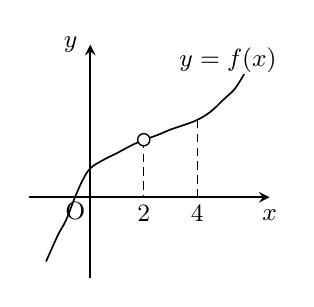
\begin{tikzpicture}[x=0.34cm, y=0.34cm, line width=0.6pt]
  \draw[->, >=stealth, line width=0.7pt] (-2.3,0) -- (6.7,0) node[below=1pt, font=\small] {$x$};
  \draw[->, >=stealth, line width=0.7pt] (0,-3.0) -- (0,5.7) node[left=1pt, font=\small] {$y$};
  \draw[densely dashed, line width=0.4pt] (2,2.15) -- (2,0);
  \draw[densely dashed, line width=0.4pt] (4,2.89) -- (4,0);
  \draw[line width=0.6pt] plot[smooth, tension=0.6] coordinates {(-1.65,-2.4) (-1.2,-1.4) (-0.9,-0.85) (-0.57,0) (-0.3,0.6) (0,1.08) (0.5,1.4) (1,1.65) (1.5,1.92) (2,2.15)};
  \draw[line width=0.6pt] plot[smooth, tension=0.6] coordinates {(2,2.15) (2.5,2.32) (3,2.53) (3.5,2.7) (4,2.89) (4.5,3.2) (5,3.67) (5.4,4.05) (5.75,4.6)};
  \draw[fill=white, line width=0.5pt] (2,2.15) circle (2.2pt);
  \node[font=\small, inner sep=2.5pt, below] at (2,0) {$2$};
  \node[font=\small, inner sep=2.5pt, below] at (4,0) {$4$};
  \node[font=\small, inner sep=1.5pt, below left] at (0,0) {$\pt{O}$};
  \node[font=\small, anchor=west, inner sep=1pt] at (3.2,5.1) {$y=f(x)$};
\end{tikzpicture}
}\end{minipage}\par
}\vspace{8mm}
\setcounter{dmproblemcount}{34}\dmpnum{33-35}{% id: 33-35
% book: 베이직쎈 미적분1 · 02 함수의 연속
% section: 개념 15 연속함수
% passage: 함수 $y=f(x)$의 그래프가 다음 그림과 같을 때, 함수 $f(x)$가 주어진 구간에서 연속함수인 것은 ‘$\bigcirc$’를, 연속함수가 아닌 것은 ‘$\times$’를 (\hspace*{1.2em}) 안에 써넣으시오.
% figure: tikz:fig-33-35
% answer: 
% answer_source: 
% variant_level: 0 (원본 전사)
% 이 파일은 build.mjs 가 items.json 에서 만든다. 고칠 때는 items.json 을 고친다.
\smash{\raisebox{1.5mm}{\dmkichul{베이직쎈 미적분1 33쪽 35번}}}
\noindent\begin{minipage}[t]{0.58\linewidth}\vspace{0pt}\raggedright $(-2{,}\mkern3mu\mathopen{}3)$ \hfill (\hspace*{2.4em})\end{minipage}\hfill\begin{minipage}[t]{0.4\linewidth}\vspace{0pt}\centering \resizebox{\ifdim\width>\linewidth\linewidth\else\width\fi}{!}{% 33-35(33쪽) — 35번 그림 · y=f(x) 의 그래프(x축을 점근선으로 오른쪽으로 갈수록 가파르게 커지는 곡선 · x=3 안내 점선). 스캔 화질이 낮아 TikZ 로 다시 그림.
% 원문에 있는 것만: x축 눈금 -2, 3 · y축 옆 1 · 점선 한 줄 · 라벨 y=f(x), O, x, y.
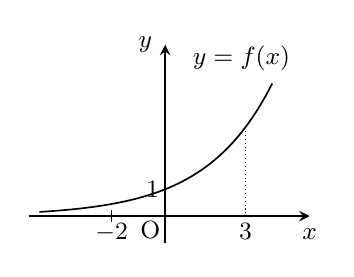
\begin{tikzpicture}[x=0.34cm, y=0.34cm, line width=0.6pt]
  \draw[->, >=stealth, line width=0.7pt] (-5.1,0) -- (5.4,0) node[below=1pt, font=\small] {$x$};
  \draw[->, >=stealth, line width=0.7pt] (0,-1.0) -- (0,6.4) node[left=1pt, font=\small] {$y$};
  \draw[densely dotted, line width=0.4pt] (3,3.32) -- (3,0);
  \draw[line width=0.6pt, domain=-4.7:4.0, samples=100, smooth] plot (\x, {exp(0.4*\x)});
  \draw[line width=0.5pt] (-2,-0.22) -- (-2,0.22);
  \node[font=\small, inner sep=2.5pt, below] at (-2,0) {$-2$};
  \node[font=\small, inner sep=2.5pt, below] at (3,0) {$3$};
  \node[font=\small, inner sep=1.5pt, below left] at (0,0) {$\pt{O}$};
  \node[font=\small, inner sep=2pt, left] at (0,1) {$1$};
  \node[font=\small, anchor=west, inner sep=1pt] at (0.9,5.9) {$y=f(x)$};
\end{tikzpicture}
}\end{minipage}\par
}\vspace{8mm}
\setcounter{dmproblemcount}{35}\dmpnum{33-36}{% id: 33-36
% book: 베이직쎈 미적분1 · 02 함수의 연속
% section: 개념 15 연속함수
% passage: 함수 $y=f(x)$의 그래프가 다음 그림과 같을 때, 함수 $f(x)$가 주어진 구간에서 연속함수인 것은 ‘$\bigcirc$’를, 연속함수가 아닌 것은 ‘$\times$’를 (\hspace*{1.2em}) 안에 써넣으시오.
% figure: tikz:fig-33-36
% answer: 
% answer_source: 
% variant_level: 0 (원본 전사)
% 이 파일은 build.mjs 가 items.json 에서 만든다. 고칠 때는 items.json 을 고친다.
\smash{\raisebox{1.5mm}{\dmkichul{베이직쎈 미적분1 33쪽 36번}}}
\noindent\begin{minipage}[t]{0.58\linewidth}\vspace{0pt}\raggedright $[-1{,}\mkern3mu\mathopen{}1]$ \hfill (\hspace*{2.4em})\end{minipage}\hfill\begin{minipage}[t]{0.4\linewidth}\vspace{0pt}\centering \resizebox{\ifdim\width>\linewidth\linewidth\else\width\fi}{!}{% 33-36(33쪽) — 36번 그림 · y=f(x) 의 그래프(원점 대칭 쌍곡선 · x축·y축이 점근선 · (1,1), (-1,-1) 안내 점선). 스캔 화질이 낮아 TikZ 로 다시 그림.
% 원문에 있는 것만: x축 눈금 -1, 1 · y축 옆 1, -1 · 점선 네 줄 · 라벨 y=f(x), O, x, y (점 표시는 원문에 없다).
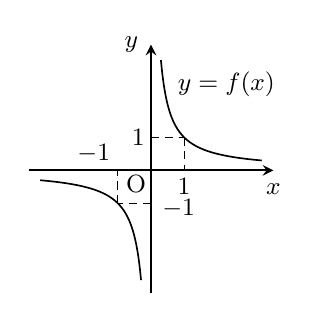
\begin{tikzpicture}[x=0.42cm, y=0.42cm, line width=0.6pt]
  \draw[->, >=stealth, line width=0.7pt] (-3.7,0) -- (3.7,0) node[below=1pt, font=\small] {$x$};
  \draw[->, >=stealth, line width=0.7pt] (0,-3.7) -- (0,3.8) node[left=1pt, font=\small] {$y$};
  \draw[densely dashed, line width=0.4pt] (0,1) -- (1,1);
  \draw[densely dashed, line width=0.4pt] (1,1) -- (1,0);
  \draw[densely dashed, line width=0.4pt] (0,-1) -- (-1,-1);
  \draw[densely dashed, line width=0.4pt] (-1,-1) -- (-1,0);
  \draw[line width=0.6pt, domain=0.30:3.35, samples=120, smooth] plot (\x, {1/\x});
  \draw[line width=0.6pt, domain=-3.35:-0.30, samples=120, smooth] plot (\x, {1/\x});
  \node[font=\small, inner sep=2.5pt, above left] at (-1,0) {$-1$};
  \node[font=\small, inner sep=2.5pt, below] at (1,0) {$1$};
  \node[font=\small, inner sep=1.5pt, below left] at (0,0) {$\pt{O}$};
  \node[font=\small, inner sep=2pt, left] at (0,1) {$1$};
  \node[font=\small, inner sep=2pt, anchor=west] at (0.15,-1.15) {$-1$};
  \node[font=\small, anchor=west, inner sep=1pt] at (0.7,2.6) {$y=f(x)$};
\end{tikzpicture}
}\end{minipage}\par
}\vspace{8mm}
\dmpassage{다음 함수 $f(x)$가 연속인 구간을 구하시오.}
\setcounter{dmproblemcount}{36}\dmpnum{33-37}{% id: 33-37
% book: 베이직쎈 미적분1 · 02 함수의 연속
% section: 개념 15 연속함수
% passage: 다음 함수 $f(x)$가 연속인 구간을 구하시오.
% figure: none
% answer: 
% answer_source: 
% variant_level: 0 (원본 전사)
% 이 파일은 build.mjs 가 items.json 에서 만든다. 고칠 때는 items.json 을 고친다.
\smash{\raisebox{1.5mm}{\dmkichul{베이직쎈 미적분1 33쪽 37번}}}
$f(x)=x^2+2$
}\vspace{8mm}
\vspace{3mm}\setcounter{dmproblemcount}{37}\dmpnum{33-38}{% id: 33-38
% book: 베이직쎈 미적분1 · 02 함수의 연속
% section: 개념 15 연속함수
% passage: 다음 함수 $f(x)$가 연속인 구간을 구하시오.
% figure: none
% answer: 
% answer_source: 
% variant_level: 0 (원본 전사)
% 이 파일은 build.mjs 가 items.json 에서 만든다. 고칠 때는 items.json 을 고친다.
\smash{\raisebox{4.5mm}{\dmkichul{베이직쎈 미적분1 33쪽 38번}}}
$f(x)=-\dfrac{1}{x}$
}\vspace{8mm}
\vspace{3mm}\setcounter{dmproblemcount}{38}\dmpnum{33-39}{% id: 33-39
% book: 베이직쎈 미적분1 · 02 함수의 연속
% section: 개념 15 연속함수
% passage: 다음 함수 $f(x)$가 연속인 구간을 구하시오.
% figure: none
% answer: 
% answer_source: 
% variant_level: 0 (원본 전사)
% 이 파일은 build.mjs 가 items.json 에서 만든다. 고칠 때는 items.json 을 고친다.
\smash{\raisebox{4.5mm}{\dmkichul{베이직쎈 미적분1 33쪽 39번}}}
$f(x)=-\sqrt{x+1}$
}\vspace{8mm}
\dmpassage{다음 함수 $f(x)$가 모든 실수 $x$에서 연속이 되도록 하는 상수 $a$의 값을 구하시오.}
\vspace{5mm}\setcounter{dmproblemcount}{39}\dmpnum{33-40}{% id: 33-40
% book: 베이직쎈 미적분1 · 02 함수의 연속
% section: 개념 15 연속함수
% passage: 다음 함수 $f(x)$가 모든 실수 $x$에서 연속이 되도록 하는 상수 $a$의 값을 구하시오.
% figure: none
% answer: 
% answer_source: 
% variant_level: 0 (원본 전사)
% 이 파일은 build.mjs 가 items.json 에서 만든다. 고칠 때는 items.json 을 고친다.
\smash{\raisebox{6.5mm}{\dmkichul{베이직쎈 미적분1 33쪽 40번}}}
$f(x)=\begin{cases} 3x+a & (x\ge -1) \\ -x^2+6 & (x<-1) \end{cases}$
\dmhint{함수 $f(x)$가 모든 실수 $x$에서 연속이려면 $x=\blank$에서 연속이어야 한다. 즉\\ $\displaystyle\lim_{x\to -1+} f(x)=\lim_{x\to -1-} f(x)=f(\blank)$\\ 이때\\ $\displaystyle\lim_{x\to -1+} f(x)=\lim_{x\to -1+}(3x+a)=\blank+a,$\\ $\displaystyle\lim_{x\to -1-} f(x)=\lim_{x\to -1-}(-x^2+6)=\blank,$\\ $f(\blank)=\blank+a$\\ 이므로 \quad $\blank+a=5$ \quad $\therefore\ a=\blank$}
}\vspace{8mm}
\vspace{5mm}\setcounter{dmproblemcount}{40}\dmpnum{33-41}{% id: 33-41
% book: 베이직쎈 미적분1 · 02 함수의 연속
% section: 개념 15 연속함수
% passage: 다음 함수 $f(x)$가 모든 실수 $x$에서 연속이 되도록 하는 상수 $a$의 값을 구하시오.
% figure: none
% answer: 
% answer_source: 
% variant_level: 0 (원본 전사)
% 이 파일은 build.mjs 가 items.json 에서 만든다. 고칠 때는 items.json 을 고친다.
\smash{\raisebox{6.5mm}{\dmkichul{베이직쎈 미적분1 33쪽 41번}}}
$f(x)=\begin{cases} \sqrt{x-3}+1 & (x\ge 3) \\ ax-5 & (x<3) \end{cases}$
\dmhint{$\displaystyle\lim_{x\to a}\dfrac{f(x)}{g(x)}=a$ ($a$는 실수)이고 $\displaystyle\lim_{x\to a}g(x)=0$이면 $\displaystyle\lim_{x\to a}f(x)=0$임을 이용해.}
}\vspace{8mm}
\dmpassage{다음 함수 $f(x)$가 모든 실수 $x$에서 연속이 되도록 하는 상수 $a$, $b$의 값을 구하시오.}
\vspace{5mm}\setcounter{dmproblemcount}{41}\dmpnum{33-42}{% id: 33-42
% book: 베이직쎈 미적분1 · 02 함수의 연속
% section: 개념 15 연속함수
% passage: 다음 함수 $f(x)$가 모든 실수 $x$에서 연속이 되도록 하는 상수 $a$, $b$의 값을 구하시오.
% figure: none
% answer: 
% answer_source: 
% variant_level: 0 (원본 전사)
% 이 파일은 build.mjs 가 items.json 에서 만든다. 고칠 때는 items.json 을 고친다.
\smash{\raisebox{6.5mm}{\dmkichul{베이직쎈 미적분1 33쪽 42번}}}
$f(x)=\begin{cases} \dfrac{x^2+2x+a}{x-1} & (x\ne 1) \\ b & (x=1) \end{cases}$
}\vspace{8mm}
\vspace{5mm}\setcounter{dmproblemcount}{42}\dmpnum{33-43}{% id: 33-43
% book: 베이직쎈 미적분1 · 02 함수의 연속
% section: 개념 15 연속함수
% passage: 다음 함수 $f(x)$가 모든 실수 $x$에서 연속이 되도록 하는 상수 $a$, $b$의 값을 구하시오.
% figure: none
% answer: 
% answer_source: 
% variant_level: 0 (원본 전사)
% 이 파일은 build.mjs 가 items.json 에서 만든다. 고칠 때는 items.json 을 고친다.
\smash{\raisebox{6.5mm}{\dmkichul{베이직쎈 미적분1 33쪽 43번}}}
$f(x)=\begin{cases} \dfrac{x^2+ax-6}{x+2} & (x\ne -2) \\ b & (x=-2) \end{cases}$
}\vspace{8mm}
\dmsection{유형 013 함수의 연속}
\setcounter{dmproblemcount}{0}\dmpnum{34-01}{% id: 34-01
% book: 베이직쎈 미적분1 · 02 함수의 연속
% section: 유형 013 함수의 연속
% figure: none
% answer: 
% answer_source: 
% variant_level: 0 (원본 전사)
% 이 파일은 build.mjs 가 items.json 에서 만든다. 고칠 때는 items.json 을 고친다.
\smash{\raisebox{1.5mm}{\dmkichul{베이직쎈 미적분1 34쪽 01번}}}
다음 중 $x=0$에서 불연속인 함수는?
\begin{choicesii}{\rule[-3ex]{0pt}{8ex}$f(x)=-x^2+3$}{\rule[-3ex]{0pt}{8ex}$f(x)=\dfrac{1}{x+1}$}{\rule[-3ex]{0pt}{8ex}$f(x)=\sqrt{x+2}$}{\rule[-3ex]{0pt}{8ex}$f(x)=\begin{cases} \dfrac{|x|}{x} & (x\ne 0) \\ 0 & (x=0) \end{cases}$}{\rule[-3ex]{0pt}{8ex}$f(x)=\begin{cases} \dfrac{x^2+x}{x} & (x\ne 0) \\ 1 & (x=0) \end{cases}$}\end{choicesii}
}\vspace{8mm}
\vspace{5mm}\setcounter{dmproblemcount}{1}\dmpnum{34-02}{% id: 34-02
% book: 베이직쎈 미적분1 · 02 함수의 연속
% section: 유형 013 함수의 연속
% figure: none
% answer: 
% answer_source: 
% variant_level: 0 (원본 전사)
% 이 파일은 build.mjs 가 items.json 에서 만든다. 고칠 때는 items.json 을 고친다.
\smash{\raisebox{6.5mm}{\dmkichul{베이직쎈 미적분1 34쪽 02번}}}
함수 $f(x)=\begin{cases} \dfrac{x^2-9}{(x-1)(x-3)} & (x\ne 3) \\ 3 & (x=3) \end{cases}$에 대하여 옳은 것만을 \textbf{보기}에서 있는 대로 고른 것은?\bogi{ㄱ. 함수 $f(x)$는 $x=1$에서 정의되어 있다.\\ ㄴ. 함수 $f(x)$는 $x=3$에서 정의되어 있다.\\ ㄷ. $\displaystyle\lim_{x\to 3} f(x)$의 값이 존재한다.\\ ㄹ. 함수 $f(x)$는 $x=1$, $x=3$에서 모두 연속이다.}
\dmchoicesauto{}{ㄱ, ㄴ}{ㄱ, ㄷ}{ㄴ, ㄷ}{ㄴ, ㄹ}{ㄴ, ㄷ, ㄹ}
}\vspace{8mm}
\vspace{5mm}\setcounter{dmproblemcount}{2}\dmpnum{34-03}{% id: 34-03
% book: 베이직쎈 미적분1 · 02 함수의 연속
% section: 유형 013 함수의 연속
% figure: none
% answer: 
% answer_source: 
% variant_level: 0 (원본 전사)
% 이 파일은 build.mjs 가 items.json 에서 만든다. 고칠 때는 items.json 을 고친다.
\smash{\raisebox{6.5mm}{\dmkichul{베이직쎈 미적분1 34쪽 03번}}}
함수 $f(x)=\begin{cases} x^2-3x & (x\ne a) \\ 4 & (x=a) \end{cases}$가 $x=a$에서 연속이 되도록 하는 모든 실수 $a$의 값의 합을 구하시오.
}\vspace{8mm}
\dmsection{유형 014 함수의 그래프와 연속}
\setcounter{dmproblemcount}{3}\dmpnum{34-04}{% id: 34-04
% book: 베이직쎈 미적분1 · 02 함수의 연속
% section: 유형 014 함수의 그래프와 연속
% figure: tikz:fig-34-04
% answer: 
% answer_source: 
% variant_level: 0 (원본 전사)
% 이 파일은 build.mjs 가 items.json 에서 만든다. 고칠 때는 items.json 을 고친다.
\smash{\raisebox{1.5mm}{\dmkichul{베이직쎈 미적분1 34쪽 04번}}}
\noindent\begin{minipage}[t]{0.58\linewidth}\vspace{0pt}\raggedright 함수 $y=f(x)$의 그래프가 오른쪽 그림과 같을 때, 구간 $(-2{,}\mkern3mu\mathopen{}2)$에서 함수 $f(x)$의 극한값이 존재하지 않는 $x$의 값의 개수를 $a$, $f(x)$가 불연속인 $x$의 값의 개수를 $b$라 하자. $a-b$의 값을 구하시오.\end{minipage}\hfill\begin{minipage}[t]{0.4\linewidth}\vspace{0pt}\centering \resizebox{\ifdim\width>\linewidth\linewidth\else\width\fi}{!}{% 34-04(34쪽) — $y=f(x)$ 의 그래프(구간 $(-2,\,2)$ 안의 극한·연속을 묻는 문항). 스캔 화질이 낮아 TikZ 로 다시 그림.
% 원문에 있는 것만: 빈 점 $(-1,\,1)$·$(0,\,2)$ · 채운 점 $(-1,\,0)$·$(0,\,1)$ · 점선 · 라벨 $-2$, $-1$, $1$, $2$, $1$, $2$, O, x, y, $y=f(x)$(눈금은 만들지 않는다).
\begin{tikzpicture}[x=0.66cm, y=0.66cm, line width=0.6pt]
  \draw[->, >=stealth, line width=0.7pt] (-2.75,0) -- (2.95,0) node[below=1pt, font=\small] {$x$};
  \draw[->, >=stealth, line width=0.7pt] (0,-0.95) -- (0,2.8) node[left=1pt, font=\small] {$y$};
  \draw[densely dashed, line width=0.4pt] (-2,0) -- (-2,1);
  \draw[densely dashed, line width=0.4pt] (-1,0) -- (-1,1);
  \draw[densely dashed, line width=0.4pt] (2,0) -- (2,1);
  \draw[densely dashed, line width=0.4pt] (-2,1) -- (2,1);
  \draw[domain=-2.45:-1, samples=60, smooth] plot (\x, {(\x+1)*(\x+1)});
  \draw (-1,1) -- (0,2) -- (1,0) -- (2.6,1.6);
  \fill (-1,0) circle (2.2pt);
  \draw[fill=white] (-1,1) circle (2.2pt);
  \draw[fill=white] (0,2) circle (2.2pt);
  \fill (0,1) circle (2.2pt);
  \node[below=1pt, font=\small] at (-2,0) {$-2$};
  \node[below=1pt, font=\small] at (-1,0) {$-1$};
  \node[below=1pt, font=\small] at (1,0) {$1$};
  \node[below=1pt, font=\small] at (2,0) {$2$};
  \node[below left=-2pt and -4pt, font=\small] at (0,0) {$\pt{O}$};
  \node[left=2pt, font=\small] at (0,2) {$2$};
  \node[below left=-1pt and -2pt, font=\small] at (0,1) {$1$};
  \node[anchor=west, font=\small] at (1.05,2.45) {$y=f(x)$};
\end{tikzpicture}
}\end{minipage}\par
}\vspace{8mm}
\setcounter{dmproblemcount}{4}\dmpnum{34-05}{% id: 34-05
% book: 베이직쎈 미적분1 · 02 함수의 연속
% section: 유형 014 함수의 그래프와 연속
% figure: tikz:fig-34-05
% answer: 
% answer_source: 
% variant_level: 0 (원본 전사)
% 이 파일은 build.mjs 가 items.json 에서 만든다. 고칠 때는 items.json 을 고친다.
\smash{\raisebox{1.5mm}{\dmkichul{베이직쎈 미적분1 34쪽 05번}}}
\noindent\begin{minipage}[t]{0.58\linewidth}\vspace{0pt}\raggedright 구간 $(0{,}\mkern3mu\mathopen{}4)$에서 함수 $y=f(x)$의 그래프가 오른쪽 그림과 같을 때, 옳은 것만을 \textbf{보기}에서 있는 대로 고른 것은?\end{minipage}\hfill\begin{minipage}[t]{0.4\linewidth}\vspace{0pt}\centering \resizebox{\ifdim\width>\linewidth\linewidth\else\width\fi}{!}{% 34-05(34쪽) — 구간 $(0,\,4)$ 에서 $y=f(x)$ 의 그래프. 스캔 화질이 낮아 TikZ 로 다시 그림.
% 원문에 있는 것만: 빈 점 $(0,\,0)$·$(1,\,1)$·$(3,\,2)$·$(4,\,3)$ · 채운 점 $(3,\,3)$ · 점선 · 라벨 $1$, $2$, $3$, $4$, O, x, y, $y=f(x)$(눈금은 만들지 않는다).
\begin{tikzpicture}[x=0.62cm, y=0.62cm, line width=0.6pt]
  \draw[->, >=stealth, line width=0.7pt] (-0.55,0) -- (5.05,0) node[below=1pt, font=\small] {$x$};
  \draw[->, >=stealth, line width=0.7pt] (0,-0.9) -- (0,4.05) node[left=1pt, font=\small] {$y$};
  \draw[densely dashed, line width=0.4pt] (0,1) -- (1,1);
  \draw[densely dashed, line width=0.4pt] (0,2) -- (3,2);
  \draw[densely dashed, line width=0.4pt] (0,3) -- (3,3);
  \draw[densely dashed, line width=0.4pt] (1,0) -- (1,1);
  \draw[densely dashed, line width=0.4pt] (2,0) -- (2,3);
  \draw[densely dashed, line width=0.4pt] (3,0) -- (3,3);
  \draw[densely dashed, line width=0.4pt] (4,0) -- (4,3);
  \draw (0,0) -- (1,1);
  \draw[domain=1:2, samples=40, smooth] plot (\x, {3-2*(2-\x)*(2-\x)});
  \draw[domain=2:3, samples=40, smooth] plot (\x, {3-(\x-2)*(\x-2)});
  \draw (3,3) -- (4,3);
  \draw[fill=white] (0,0) circle (2.2pt);
  \draw[fill=white] (1,1) circle (2.2pt);
  \draw[fill=white] (3,2) circle (2.2pt);
  \fill (3,3) circle (2.2pt);
  \draw[fill=white] (4,3) circle (2.2pt);
  \node[below=1pt, font=\small] at (1,0) {$1$};
  \node[below=1pt, font=\small] at (2,0) {$2$};
  \node[below=1pt, font=\small] at (3,0) {$3$};
  \node[below=1pt, font=\small] at (4,0) {$4$};
  \node[below left=-2pt and -4pt, font=\small] at (0,0) {$\pt{O}$};
  \node[left=2pt, font=\small] at (0,1) {$1$};
  \node[left=2pt, font=\small] at (0,2) {$2$};
  \node[left=2pt, font=\small] at (0,3) {$3$};
  \node[anchor=west, font=\small] at (2.55,3.75) {$y=f(x)$};
\end{tikzpicture}
}\end{minipage}\par
\noindent \bogi{ㄱ. $\displaystyle\lim_{x\to 1-} f(x)=1$\\ ㄴ. $\displaystyle\lim_{x\to 3} f(x)$의 값이 존재한다.\\ ㄷ. 함수 $f(x)$는 $x=2$에서 연속이다.\\ ㄹ. 구간 $(0{,}\mkern3mu\mathopen{}4)$에서 함수 $f(x)$가 불연속인 모든 $x$의 값의 합은 6이다.}
\dmchoicesauto{}{ㄱ, ㄴ}{ㄱ, ㄷ}{ㄴ, ㄷ}{ㄱ, ㄷ, ㄹ}{ㄴ, ㄷ, ㄹ}
}\vspace{8mm}
\setcounter{dmproblemcount}{5}\dmpnum{34-06}{% id: 34-06
% book: 베이직쎈 미적분1 · 02 함수의 연속
% section: 유형 014 함수의 그래프와 연속
% figure: tikz:fig-34-06
% answer: 
% answer_source: 
% variant_level: 0 (원본 전사)
% 이 파일은 build.mjs 가 items.json 에서 만든다. 고칠 때는 items.json 을 고친다.
\smash{\raisebox{1.5mm}{\dmkichul{베이직쎈 미적분1 34쪽 06번}}}
두 함수 $y=f(x)$, $y=g(x)$의 그래프가 아래 그림과 같을 때, 다음에 답하시오.
\par\smallskip\begin{center}\resizebox{\ifdim\width>\linewidth\linewidth\else\width\fi}{!}{% 34-06(34쪽) — $y=f(x)$ 와 $y=g(x)$ 의 그래프 둘(원문처럼 나란히). 스캔 화질이 낮아 TikZ 로 다시 그림.
% 원문에 있는 것만: 왼쪽 채운 점 $(1,\,1)$·빈 점 $(1,\,-1)$, 오른쪽 빈 점 $(1,\,1)$·채운 점 $(1,\,-1)$ · 점선 · 라벨 $1$, $-1$, O, x, y, $y=f(x)$, $y=g(x)$(눈금은 만들지 않는다).
\begin{tikzpicture}[x=0.62cm, y=0.62cm, line width=0.6pt]
  \begin{scope}
    \draw[->, >=stealth, line width=0.7pt] (-1.95,0) -- (3.0,0) node[below=1pt, font=\small] {$x$};
    \draw[->, >=stealth, line width=0.7pt] (0,-1.95) -- (0,1.95) node[left=1pt, font=\small] {$y$};
    \draw[densely dashed, line width=0.4pt] (0,1) -- (1,1);
    \draw[densely dashed, line width=0.4pt] (1,1) -- (1,-1);
    \draw (-1.7,-1) -- (1,-1);
    \draw (1,1) -- (2.75,1);
    \fill (1,1) circle (2.2pt);
    \draw[fill=white] (1,-1) circle (2.2pt);
    \node[left=2pt, font=\small] at (0,1) {$1$};
    \node[below left=-2pt and -3pt, font=\small] at (0,-1) {$-1$};
    \node[below right=-1pt and -2pt, font=\small] at (1,0) {$1$};
    \node[below left=-2pt and -4pt, font=\small] at (0,0) {$\pt{O}$};
    \node[anchor=west, font=\small] at (0.75,1.7) {$y=f(x)$};
  \end{scope}
  \begin{scope}[shift={(6.6,0)}]
    \draw[->, >=stealth, line width=0.7pt] (-2.2,0) -- (3.0,0) node[below=1pt, font=\small] {$x$};
    \draw[->, >=stealth, line width=0.7pt] (0,-1.95) -- (0,1.95) node[left=1pt, font=\small] {$y$};
    \draw[densely dashed, line width=0.4pt] (0,-1) -- (1,-1);
    \draw[densely dashed, line width=0.4pt] (1,1) -- (1,-1);
    \draw (-1.95,1) -- (1,1);
    \draw (1,-1) -- (2.75,-1);
    \draw[fill=white] (1,1) circle (2.2pt);
    \fill (1,-1) circle (2.2pt);
    \node[above left=-3pt and -2pt, font=\small] at (0,1) {$1$};
    \node[left=2pt, font=\small] at (0,-1) {$-1$};
    \node[below right=-1pt and -2pt, font=\small] at (1,0) {$1$};
    \node[below left=-2pt and -4pt, font=\small] at (0,0) {$\pt{O}$};
    \node[anchor=west, font=\small] at (0.75,1.7) {$y=g(x)$};
  \end{scope}
\end{tikzpicture}
}\end{center}
\dmsubprob{1} $f(1)g(1)$의 값을 구하시오.
\dmsubprob{2} 극한 $\displaystyle\lim_{x\to 1} f(x)g(x)$를 조사하시오.
\dmsubprob{3} 함수 $f(x)g(x)$가 $x=1$에서 연속인지 불연속인지 조사하시오.
}\vspace{8mm}
\dmsection{유형 015 미정계수의 결정}
\vspace{5mm}\setcounter{dmproblemcount}{6}\dmpnum{35-07}{% id: 35-07
% book: 베이직쎈 미적분1 · 02 함수의 연속
% section: 유형 015 미정계수의 결정
% figure: none
% answer: 
% answer_source: 
% variant_level: 0 (원본 전사)
% 이 파일은 build.mjs 가 items.json 에서 만든다. 고칠 때는 items.json 을 고친다.
\smash{\raisebox{6.5mm}{\dmkichul{베이직쎈 미적분1 35쪽 07번}}}
함수 $f(x)=\begin{cases} \dfrac{x^3-4x+3}{x-1} & (x\ne 1) \\ k & (x=1) \end{cases}$가 $x=1$에서 연속이 되도록 하는 상수 $k$의 값을 구하시오.
}\vspace{8mm}
\vspace{5mm}\setcounter{dmproblemcount}{7}\dmpnum{35-08}{% id: 35-08
% book: 베이직쎈 미적분1 · 02 함수의 연속
% section: 유형 015 미정계수의 결정
% figure: none
% answer: 
% answer_source: 
% variant_level: 0 (원본 전사)
% 이 파일은 build.mjs 가 items.json 에서 만든다. 고칠 때는 items.json 을 고친다.
\smash{\raisebox{6.5mm}{\dmkichul{베이직쎈 미적분1 35쪽 08번}}}
함수 $f(x)=\begin{cases} \sqrt{x+3} & (x\ge -2) \\ -x^2+2x+a & (x<-2) \end{cases}$가 모든 실수 $x$에서 연속이 되도록 하는 상수 $a$의 값은?
\dmchoicesauto{}{$5$}{$7$}{$9$}{$11$}{$13$}
}\vspace{8mm}
\vspace{5mm}\setcounter{dmproblemcount}{8}\dmpnum{35-09}{% id: 35-09
% book: 베이직쎈 미적분1 · 02 함수의 연속
% section: 유형 015 미정계수의 결정
% figure: none
% answer: 
% answer_source: 
% variant_level: 0 (원본 전사)
% 이 파일은 build.mjs 가 items.json 에서 만든다. 고칠 때는 items.json 을 고친다.
\smash{\raisebox{6.5mm}{\dmkichul{베이직쎈 미적분1 35쪽 09번}}}
함수 $f(x)=\begin{cases} \dfrac{a\sqrt{x+1}+b}{x-3} & (x>3) \\ 1 & (x\le 3) \end{cases}$이 모든 실수 $x$에서 연속이 되도록 하는 상수 $a$, $b$에 대하여 $a+b$의 값을 구하시오.
}\vspace{8mm}
\vspace{5mm}\setcounter{dmproblemcount}{9}\dmpnum{35-10}{% id: 35-10
% book: 베이직쎈 미적분1 · 02 함수의 연속
% section: 유형 015 미정계수의 결정
% figure: none
% answer: 
% answer_source: 
% variant_level: 0 (원본 전사)
% 이 파일은 build.mjs 가 items.json 에서 만든다. 고칠 때는 items.json 을 고친다.
\smash{\raisebox{6.5mm}{\dmkichul{베이직쎈 미적분1 35쪽 10번}}}
함수 $f(x)=\begin{cases} -x^2-x & (|x|\ge 1) \\ x^2+ax+b & (|x|<1) \end{cases}$가 실수 전체의 집합에서 연속이 되도록 하는 상수 $a$, $b$에 대하여 $ab$의 값은?
\dmchoicesauto{}{$-4$}{$-2$}{$-1$}{$1$}{$2$}
}\vspace{8mm}
\dmsection{유형 016 $(x-a)f(x)=g(x)$ 꼴의 함수의 연속}
\setcounter{dmproblemcount}{10}\dmpnum{35-11}{% id: 35-11
% book: 베이직쎈 미적분1 · 02 함수의 연속
% section: 유형 016 $(x-a)f(x)=g(x)$ 꼴의 함수의 연속
% figure: none
% answer: 
% answer_source: 
% variant_level: 0 (원본 전사)
% 이 파일은 build.mjs 가 items.json 에서 만든다. 고칠 때는 items.json 을 고친다.
\smash{\raisebox{1.5mm}{\dmkichul{베이직쎈 미적분1 35쪽 11번}}}
모든 실수 $x$에서 연속인 함수 $f(x)$가\par\smallskip\dispeq{$(x+1)f(x)=x^2-1$}\par\smallskip\noindent 을 만족시킬 때, 다음을 구하시오.
\dmsubprob{1} $x\ne -1$일 때, 함수 $f(x)$
\dmsubprob{2} $f(-1)$의 값
}\vspace{8mm}
\setcounter{dmproblemcount}{11}\dmpnum{35-12}{% id: 35-12
% book: 베이직쎈 미적분1 · 02 함수의 연속
% section: 유형 016 $(x-a)f(x)=g(x)$ 꼴의 함수의 연속
% figure: none
% answer: 
% answer_source: 
% variant_level: 0 (원본 전사)
% 이 파일은 build.mjs 가 items.json 에서 만든다. 고칠 때는 items.json 을 고친다.
\smash{\raisebox{1.5mm}{\dmkichul{베이직쎈 미적분1 35쪽 12번}}}
모든 실수 $x$에서 연속인 함수 $f(x)$가\par\smallskip\dispeq{$(x-3)f(x)=x^2+ax-15$}\par\smallskip\noindent 를 만족시킬 때, $f(3)$의 값은? \dmcondfill{$a$는 상수이다.}{}
\dmchoicesauto{}{$2$}{$4$}{$6$}{$8$}{$10$}
}\vspace{8mm}
\vspace{3mm}\setcounter{dmproblemcount}{12}\dmpnum{35-13}{% id: 35-13
% book: 베이직쎈 미적분1 · 02 함수의 연속
% section: 유형 016 $(x-a)f(x)=g(x)$ 꼴의 함수의 연속
% figure: none
% answer: 
% answer_source: 
% variant_level: 0 (원본 전사)
% 이 파일은 build.mjs 가 items.json 에서 만든다. 고칠 때는 items.json 을 고친다.
\smash{\raisebox{4.5mm}{\dmkichul{베이직쎈 미적분1 35쪽 13번}}}
$x\ge -7$인 모든 실수 $x$에서 연속인 함수 $f(x)$가\par\smallskip\dispeq{$(x-2)f(x)=\sqrt{x+7}-a$}\par\smallskip\noindent 를 만족시킬 때, $f(2)$의 값은? \dmcondfill{$a$는 상수이다.}{}
\dmchoicesauto{\rule[-3ex]{0pt}{8ex}}{$\dfrac{1}{12}$}{$\dfrac{1}{6}$}{$\dfrac{1}{3}$}{$\dfrac{2}{3}$}{$1$}
}\vspace{8mm}
\dmsection{개념 16 연속함수의 성질}
\dmpassage{다음 함수 $f(x)$의 연속성을 조사하시오.}
\setcounter{dmproblemcount}{0}\dmpnum{36-01}{% id: 36-01
% book: 베이직쎈 미적분1 · 02 함수의 연속
% section: 개념 16 연속함수의 성질
% passage: 다음 함수 $f(x)$의 연속성을 조사하시오.
% figure: none
% answer: 
% answer_source: 
% variant_level: 0 (원본 전사)
% 이 파일은 build.mjs 가 items.json 에서 만든다. 고칠 때는 items.json 을 고친다.
\smash{\raisebox{1.5mm}{\dmkichul{베이직쎈 미적분1 36쪽 01번}}}
$f(x)=2x^2-x+5$
}\vspace{8mm}
\setcounter{dmproblemcount}{1}\dmpnum{36-02}{% id: 36-02
% book: 베이직쎈 미적분1 · 02 함수의 연속
% section: 개념 16 연속함수의 성질
% passage: 다음 함수 $f(x)$의 연속성을 조사하시오.
% figure: none
% answer: 
% answer_source: 
% variant_level: 0 (원본 전사)
% 이 파일은 build.mjs 가 items.json 에서 만든다. 고칠 때는 items.json 을 고친다.
\smash{\raisebox{1.5mm}{\dmkichul{베이직쎈 미적분1 36쪽 02번}}}
$f(x)=(x+4)(x-3)$
}\vspace{8mm}
\vspace{3mm}\setcounter{dmproblemcount}{2}\dmpnum{36-03}{% id: 36-03
% book: 베이직쎈 미적분1 · 02 함수의 연속
% section: 개념 16 연속함수의 성질
% passage: 다음 함수 $f(x)$의 연속성을 조사하시오.
% figure: none
% answer: 
% answer_source: 
% variant_level: 0 (원본 전사)
% 이 파일은 build.mjs 가 items.json 에서 만든다. 고칠 때는 items.json 을 고친다.
\smash{\raisebox{4.5mm}{\dmkichul{베이직쎈 미적분1 36쪽 03번}}}
$f(x)=\dfrac{x-2}{x+1}$
}\vspace{8mm}
\dmpassage{다음 함수 $f(x)$가 연속인 구간을 구하시오.}
\setcounter{dmproblemcount}{3}\dmpnum{36-04}{% id: 36-04
% book: 베이직쎈 미적분1 · 02 함수의 연속
% section: 개념 16 연속함수의 성질
% passage: 다음 함수 $f(x)$가 연속인 구간을 구하시오.
% figure: none
% answer: 
% answer_source: 
% variant_level: 0 (원본 전사)
% 이 파일은 build.mjs 가 items.json 에서 만든다. 고칠 때는 items.json 을 고친다.
\smash{\raisebox{1.5mm}{\dmkichul{베이직쎈 미적분1 36쪽 04번}}}
$f(x)=x^3+x^2-x+1$
}\vspace{8mm}
\vspace{3mm}\setcounter{dmproblemcount}{4}\dmpnum{36-05}{% id: 36-05
% book: 베이직쎈 미적분1 · 02 함수의 연속
% section: 개념 16 연속함수의 성질
% passage: 다음 함수 $f(x)$가 연속인 구간을 구하시오.
% figure: none
% answer: 
% answer_source: 
% variant_level: 0 (원본 전사)
% 이 파일은 build.mjs 가 items.json 에서 만든다. 고칠 때는 items.json 을 고친다.
\smash{\raisebox{4.5mm}{\dmkichul{베이직쎈 미적분1 36쪽 05번}}}
$f(x)=\dfrac{x^2}{x-2}$
}\vspace{8mm}
\vspace{3mm}\setcounter{dmproblemcount}{5}\dmpnum{36-06}{% id: 36-06
% book: 베이직쎈 미적분1 · 02 함수의 연속
% section: 개념 16 연속함수의 성질
% passage: 다음 함수 $f(x)$가 연속인 구간을 구하시오.
% figure: none
% answer: 
% answer_source: 
% variant_level: 0 (원본 전사)
% 이 파일은 build.mjs 가 items.json 에서 만든다. 고칠 때는 items.json 을 고친다.
\smash{\raisebox{4.5mm}{\dmkichul{베이직쎈 미적분1 36쪽 06번}}}
$f(x)=\dfrac{2}{x^2-9}$
}\vspace{8mm}
\dmpassage{두 함수 $f(x)=x+2$, $g(x)=x^2-5x$에 대하여 다음 함수가 연속인 구간을 구하시오.}
\setcounter{dmproblemcount}{6}\dmpnum{36-07}{% id: 36-07
% book: 베이직쎈 미적분1 · 02 함수의 연속
% section: 개념 16 연속함수의 성질
% passage: 두 함수 $f(x)=x+2$, $g(x)=x^2-5x$에 대하여 다음 함수가 연속인 구간을 구하시오.
% figure: none
% answer: 
% answer_source: 
% variant_level: 0 (원본 전사)
% 이 파일은 build.mjs 가 items.json 에서 만든다. 고칠 때는 items.json 을 고친다.
\smash{\raisebox{1.5mm}{\dmkichul{베이직쎈 미적분1 36쪽 07번}}}
$-2f(x)$
}\vspace{8mm}
\setcounter{dmproblemcount}{7}\dmpnum{36-08}{% id: 36-08
% book: 베이직쎈 미적분1 · 02 함수의 연속
% section: 개념 16 연속함수의 성질
% passage: 두 함수 $f(x)=x+2$, $g(x)=x^2-5x$에 대하여 다음 함수가 연속인 구간을 구하시오.
% figure: none
% answer: 
% answer_source: 
% variant_level: 0 (원본 전사)
% 이 파일은 build.mjs 가 items.json 에서 만든다. 고칠 때는 items.json 을 고친다.
\smash{\raisebox{1.5mm}{\dmkichul{베이직쎈 미적분1 36쪽 08번}}}
$f(x)+g(x)$
}\vspace{8mm}
\setcounter{dmproblemcount}{8}\dmpnum{36-09}{% id: 36-09
% book: 베이직쎈 미적분1 · 02 함수의 연속
% section: 개념 16 연속함수의 성질
% passage: 두 함수 $f(x)=x+2$, $g(x)=x^2-5x$에 대하여 다음 함수가 연속인 구간을 구하시오.
% figure: none
% answer: 
% answer_source: 
% variant_level: 0 (원본 전사)
% 이 파일은 build.mjs 가 items.json 에서 만든다. 고칠 때는 items.json 을 고친다.
\smash{\raisebox{1.5mm}{\dmkichul{베이직쎈 미적분1 36쪽 09번}}}
$f(x)-g(x)$
}\vspace{8mm}
\setcounter{dmproblemcount}{9}\dmpnum{36-10}{% id: 36-10
% book: 베이직쎈 미적분1 · 02 함수의 연속
% section: 개념 16 연속함수의 성질
% passage: 두 함수 $f(x)=x+2$, $g(x)=x^2-5x$에 대하여 다음 함수가 연속인 구간을 구하시오.
% figure: none
% answer: 
% answer_source: 
% variant_level: 0 (원본 전사)
% 이 파일은 build.mjs 가 items.json 에서 만든다. 고칠 때는 items.json 을 고친다.
\smash{\raisebox{1.5mm}{\dmkichul{베이직쎈 미적분1 36쪽 10번}}}
$f(x)g(x)$
}\vspace{8mm}
\vspace{3mm}\setcounter{dmproblemcount}{10}\dmpnum{36-11}{% id: 36-11
% book: 베이직쎈 미적분1 · 02 함수의 연속
% section: 개념 16 연속함수의 성질
% passage: 두 함수 $f(x)=x+2$, $g(x)=x^2-5x$에 대하여 다음 함수가 연속인 구간을 구하시오.
% figure: none
% answer: 
% answer_source: 
% variant_level: 0 (원본 전사)
% 이 파일은 build.mjs 가 items.json 에서 만든다. 고칠 때는 items.json 을 고친다.
\smash{\raisebox{4.5mm}{\dmkichul{베이직쎈 미적분1 36쪽 11번}}}
$\dfrac{g(x)}{f(x)}$
}\vspace{8mm}
\vspace{3mm}\setcounter{dmproblemcount}{11}\dmpnum{36-12}{% id: 36-12
% book: 베이직쎈 미적분1 · 02 함수의 연속
% section: 개념 16 연속함수의 성질
% passage: 두 함수 $f(x)=x+2$, $g(x)=x^2-5x$에 대하여 다음 함수가 연속인 구간을 구하시오.
% figure: none
% answer: 
% answer_source: 
% variant_level: 0 (원본 전사)
% 이 파일은 build.mjs 가 items.json 에서 만든다. 고칠 때는 items.json 을 고친다.
\smash{\raisebox{4.5mm}{\dmkichul{베이직쎈 미적분1 36쪽 12번}}}
$\dfrac{f(x)}{g(x)}$
}\vspace{8mm}
\dmsection{개념 17 최대·최소 정리}
\dmpassage{함수 $y=f(x)$의 그래프가 아래 그림과 같을 때, 함수 $f(x)$가 다음 구간에서 최댓값 또는 최솟값을 가지면 그 값을 구하시오.}
\begin{center}\resizebox{\ifdim\width>\linewidth\linewidth\else\width\fi}{!}{% 37-13(37쪽) — 13~18번 공통 그림 · $y=f(x)$ 의 그래프($x=2$ 에서 끊겨 $(2,0)$ 은 채운 점, $(2,-1)$ 은 빈 점 · $(4,3)$ 은 빈 점). 스캔 화질이 낮아 TikZ 로 다시 그림.
% 원문에 있는 것만 옮긴다: 눈금 -5, -4, -1, 1, 2, 3, 4, 5, 7 과 -1, 2, 3, 4 · 점선 · 라벨 O, x, y, y=f(x). 원문에 없는 값은 적지 않는다.
\begin{tikzpicture}[x=0.42cm, y=0.42cm, line width=0.6pt]
  \draw[->, >=stealth, line width=0.7pt] (-6.6,0) -- (8.7,0) node[below=2pt, font=\small] {$x$};
  \draw[->, >=stealth, line width=0.7pt] (0,-2.5) -- (0,5.1) node[left=1pt, font=\small] {$y$};
  \draw[densely dashed, line width=0.4pt] (-4,0) -- (-4,-1) -- (2,-1);
  \draw[densely dashed, line width=0.4pt] (-1,0) -- (-1,2) -- (0,2);
  \draw[densely dashed, line width=0.4pt] (1,0) -- (1,4);
  \draw[densely dashed, line width=0.4pt] (0,4) -- (5,4) -- (5,0);
  \draw[densely dashed, line width=0.4pt] (0,3) -- (4,3) -- (4,0);
  \draw[densely dashed, line width=0.4pt] (2,0) -- (2,-1);
  \draw plot[smooth, tension=0.75] coordinates {(-6.05,1.45) (-5.4,0.65) (-4.8,-0.2) (-4.3,-0.82) (-4,-1) (-3.7,-0.82) (-3.2,-0.25) (-3,0) (-2,1) (-1,2) (0,3) (0.55,3.65) (1,4) (1.4,3.72) (1.7,2.9) (1.88,1.7) (2,0)};
  \draw plot[smooth, tension=0.75] coordinates {(2,-1) (2.4,-0.5) (2.75,0) (3.2,1.0) (3.6,2.0) (4,3.0) (4.5,3.7) (5,4) (5.5,3.45) (6,2.5) (6.5,1.5) (7,0) (7.5,-0.75) (8.1,-1.1)};
  \fill (2,0) circle (2.2pt);
  \draw[fill=white, line width=0.5pt] (2,-1) circle (2.2pt);
  \draw[fill=white, line width=0.5pt] (4,3) circle (2.2pt);
  \node[below left=-2pt and -4pt, font=\small] at (-5,0) {$-5$};
  \node[above left=-2pt and -4pt, font=\small] at (-4,0) {$-4$};
  \node[below=1pt, font=\small] at (-1,0) {$-1$};
  \node[below right=-2pt and -3pt, font=\small] at (0,0) {$\pt{O}$};
  \node[below=1pt, font=\small] at (1,0) {$1$};
  \node[below left=-2pt and -4pt, font=\small] at (2,0) {$2$};
  \node[below=1pt, font=\small] at (3,0) {$3$};
  \node[below=1pt, font=\small] at (4,0) {$4$};
  \node[below=1pt, font=\small] at (5,0) {$5$};
  \node[below=1pt, font=\small] at (7,0) {$7$};
  \node[left=1pt, font=\small] at (0,4) {$4$};
  \node[left=1pt, font=\small] at (0,3) {$3$};
  \node[right=1pt, font=\small] at (0,2) {$2$};
  \node[font=\small] at (-0.8,-1.5) {$-1$};
  \node[font=\small] at (4.8,4.85) {$y=f(x)$};
\end{tikzpicture}
}\end{center}\vspace{4mm}
\setcounter{dmproblemcount}{12}\dmpnum{37-13}{% id: 37-13
% book: 베이직쎈 미적분1 · 02 함수의 연속
% section: 개념 17 최대·최소 정리
% passage: 함수 $y=f(x)$의 그래프가 아래 그림과 같을 때, 함수 $f(x)$가 다음 구간에서 최댓값 또는 최솟값을 가지면 그 값을 구하시오.
% figure: tikz:fig-37-13
% answer: 
% answer_source: 
% variant_level: 0 (원본 전사)
% 이 파일은 build.mjs 가 items.json 에서 만든다. 고칠 때는 items.json 을 고친다.
\smash{\raisebox{1.5mm}{\dmkichul{베이직쎈 미적분1 37쪽 13번}}}
$[-4{,}\mkern3mu\mathopen{}-1]$
}\vspace{8mm}
\setcounter{dmproblemcount}{13}\dmpnum{37-14}{% id: 37-14
% book: 베이직쎈 미적분1 · 02 함수의 연속
% section: 개념 17 최대·최소 정리
% passage: 함수 $y=f(x)$의 그래프가 아래 그림과 같을 때, 함수 $f(x)$가 다음 구간에서 최댓값 또는 최솟값을 가지면 그 값을 구하시오.
% figure: tikz:fig-37-13
% answer: 
% answer_source: 
% variant_level: 0 (원본 전사)
% 이 파일은 build.mjs 가 items.json 에서 만든다. 고칠 때는 items.json 을 고친다.
\smash{\raisebox{1.5mm}{\dmkichul{베이직쎈 미적분1 37쪽 14번}}}
$[1{,}\mkern3mu\mathopen{}3]$
}\vspace{8mm}
\setcounter{dmproblemcount}{14}\dmpnum{37-15}{% id: 37-15
% book: 베이직쎈 미적분1 · 02 함수의 연속
% section: 개념 17 최대·최소 정리
% passage: 함수 $y=f(x)$의 그래프가 아래 그림과 같을 때, 함수 $f(x)$가 다음 구간에서 최댓값 또는 최솟값을 가지면 그 값을 구하시오.
% figure: tikz:fig-37-13
% answer: 
% answer_source: 
% variant_level: 0 (원본 전사)
% 이 파일은 build.mjs 가 items.json 에서 만든다. 고칠 때는 items.json 을 고친다.
\smash{\raisebox{1.5mm}{\dmkichul{베이직쎈 미적분1 37쪽 15번}}}
$[2{,}\mkern3mu\mathopen{}4]$
}\vspace{8mm}
\setcounter{dmproblemcount}{15}\dmpnum{37-16}{% id: 37-16
% book: 베이직쎈 미적분1 · 02 함수의 연속
% section: 개념 17 최대·최소 정리
% passage: 함수 $y=f(x)$의 그래프가 아래 그림과 같을 때, 함수 $f(x)$가 다음 구간에서 최댓값 또는 최솟값을 가지면 그 값을 구하시오.
% figure: tikz:fig-37-13
% answer: 
% answer_source: 
% variant_level: 0 (원본 전사)
% 이 파일은 build.mjs 가 items.json 에서 만든다. 고칠 때는 items.json 을 고친다.
\smash{\raisebox{1.5mm}{\dmkichul{베이직쎈 미적분1 37쪽 16번}}}
$[-1{,}\mkern3mu\mathopen{}1)$
}\vspace{8mm}
\setcounter{dmproblemcount}{16}\dmpnum{37-17}{% id: 37-17
% book: 베이직쎈 미적분1 · 02 함수의 연속
% section: 개념 17 최대·최소 정리
% passage: 함수 $y=f(x)$의 그래프가 아래 그림과 같을 때, 함수 $f(x)$가 다음 구간에서 최댓값 또는 최솟값을 가지면 그 값을 구하시오.
% figure: tikz:fig-37-13
% answer: 
% answer_source: 
% variant_level: 0 (원본 전사)
% 이 파일은 build.mjs 가 items.json 에서 만든다. 고칠 때는 items.json 을 고친다.
\smash{\raisebox{1.5mm}{\dmkichul{베이직쎈 미적분1 37쪽 17번}}}
$(4{,}\mkern3mu\mathopen{}7]$
}\vspace{8mm}
\setcounter{dmproblemcount}{17}\dmpnum{37-18}{% id: 37-18
% book: 베이직쎈 미적분1 · 02 함수의 연속
% section: 개념 17 최대·최소 정리
% passage: 함수 $y=f(x)$의 그래프가 아래 그림과 같을 때, 함수 $f(x)$가 다음 구간에서 최댓값 또는 최솟값을 가지면 그 값을 구하시오.
% figure: tikz:fig-37-13
% answer: 
% answer_source: 
% variant_level: 0 (원본 전사)
% 이 파일은 build.mjs 가 items.json 에서 만든다. 고칠 때는 items.json 을 고친다.
\smash{\raisebox{1.5mm}{\dmkichul{베이직쎈 미적분1 37쪽 18번}}}
$(-5{,}\mkern3mu\mathopen{}2)$
}\vspace{8mm}
\dmpassage{주어진 구간에서 다음 함수 $f(x)$의 최댓값과 최솟값을 구하시오.}
\setcounter{dmproblemcount}{18}\dmpnum{37-19}{% id: 37-19
% book: 베이직쎈 미적분1 · 02 함수의 연속
% section: 개념 17 최대·최소 정리
% passage: 주어진 구간에서 다음 함수 $f(x)$의 최댓값과 최솟값을 구하시오.
% figure: tikz:fig-37-19
% answer: 
% answer_source: 
% variant_level: 0 (원본 전사)
% 이 파일은 build.mjs 가 items.json 에서 만든다. 고칠 때는 items.json 을 고친다.
\smash{\raisebox{1.5mm}{\dmkichul{베이직쎈 미적분1 37쪽 19번}}}
\noindent\begin{minipage}[t]{0.58\linewidth}\vspace{0pt}\raggedright $f(x)=x^2+1$ \qquad $[-1{,}\mkern3mu\mathopen{}2]$\end{minipage}\hfill\begin{minipage}[t]{0.4\linewidth}\vspace{0pt}\centering \resizebox{\ifdim\width>\linewidth\linewidth\else\width\fi}{!}{% 37-19(37쪽) — 19번 풀이 힌트의 그림 · $y=x^2+1$ 의 그래프(구간 $[-1,2]$ 만 실선, 밖은 점선 · 양 끝 채운 점 · 빈 네모 다섯 개). 스캔 화질이 낮아 TikZ 로 다시 그림.
% 원문에 있는 것만 옮긴다: 빈 네모(값은 학생이 채운다) · 점선 · 지시선 · 라벨 O, x, y, y=f(x). 답이 그림에서 읽히지 않게 네모는 비워 둔다.
\begin{tikzpicture}[x=0.42cm, y=0.42cm, line width=0.6pt]
  \draw[->, >=stealth, line width=0.7pt] (-3.5,0) -- (3.9,0) node[below=2pt, font=\small] {$x$};
  \draw[->, >=stealth, line width=0.7pt] (0,-2.2) -- (0,7.7) node[left=1pt, font=\small] {$y$};
  \node[below right=-2pt and 1pt, font=\small] at (0,0) {$\pt{O}$};
  \draw[densely dashed, line width=0.4pt] (-0.25,5) -- (2,5);
  \draw[densely dashed, line width=0.4pt] (2,5) -- (2,-0.2);
  \draw[densely dashed, line width=0.4pt] (-1,2) -- (-1,-0.2);
  \draw[densely dashed, line width=0.4pt] (-1,2) -- (0.25,2);
  \draw[dotted, line width=0.9pt] plot[domain=-2.43:-1, samples=40, smooth] (\x, {\x*\x+1});
  \draw[dotted, line width=0.9pt] plot[domain=2:2.44, samples=20, smooth] (\x, {\x*\x+1});
  \draw[line width=0.7pt] plot[domain=-1:2, samples=60, smooth] (\x, {\x*\x+1});
  \fill (-1,2) circle (2.2pt);
  \fill (2,5) circle (2.2pt);
  \node[draw, line width=0.4pt, inner sep=0pt, minimum width=0.48cm, minimum height=0.50cm] at (-0.8,5.05) {};
  \node[draw, line width=0.4pt, inner sep=0pt, minimum width=0.48cm, minimum height=0.50cm] at (2.95,3.0) {};
  \node[draw, line width=0.4pt, inner sep=0pt, minimum width=0.48cm, minimum height=0.50cm] at (-2.6,0.95) {};
  \node[draw, line width=0.4pt, inner sep=0pt, minimum width=0.48cm, minimum height=0.50cm] at (-1,-0.78) {};
  \node[draw, line width=0.4pt, inner sep=0pt, minimum width=0.48cm, minimum height=0.50cm] at (2,-0.78) {};
  \draw[->, >=stealth, line width=0.3pt] (2.38,3.25) .. controls (1.5,2.55) and (0.9,1.95) .. (0.3,2.05);
  \draw[line width=0.3pt] (-1.95,0.88) .. controls (-1.4,0.28) and (-0.6,0.28) .. (-0.02,1.0);
  \node[font=\small] at (2.2,7.45) {$y=f(x)$};
\end{tikzpicture}
}\end{minipage}\par
\dmhint{$f(x)=x^2+1$은 구간 $[-1{,}\mkern3mu\mathopen{}2]$에서 \blank[2.4em]이므로 이 구간에서 반드시 최댓값과 최솟값을 갖는다.\\ $y=f(x)$의 그래프는 구간 $[-1{,}\mkern3mu\mathopen{}2]$에서 오른쪽 그림과 같으므로 함수 $f(x)$는\\ $x=\blank$일 때 최댓값 \blank를 갖고,\\ $x=\blank$일 때 최솟값 \blank을 갖는다.}
}\vspace{8mm}
\setcounter{dmproblemcount}{19}\dmpnum{37-20}{% id: 37-20
% book: 베이직쎈 미적분1 · 02 함수의 연속
% section: 개념 17 최대·최소 정리
% passage: 주어진 구간에서 다음 함수 $f(x)$의 최댓값과 최솟값을 구하시오.
% figure: none
% answer: 
% answer_source: 
% variant_level: 0 (원본 전사)
% 이 파일은 build.mjs 가 items.json 에서 만든다. 고칠 때는 items.json 을 고친다.
\smash{\raisebox{1.5mm}{\dmkichul{베이직쎈 미적분1 37쪽 20번}}}
$f(x)=-x+2$ \qquad $[0{,}\mkern3mu\mathopen{}1]$
}\vspace{8mm}
\vspace{3mm}\setcounter{dmproblemcount}{20}\dmpnum{37-21}{% id: 37-21
% book: 베이직쎈 미적분1 · 02 함수의 연속
% section: 개념 17 최대·최소 정리
% passage: 주어진 구간에서 다음 함수 $f(x)$의 최댓값과 최솟값을 구하시오.
% figure: none
% answer: 
% answer_source: 
% variant_level: 0 (원본 전사)
% 이 파일은 build.mjs 가 items.json 에서 만든다. 고칠 때는 items.json 을 고친다.
\smash{\raisebox{4.5mm}{\dmkichul{베이직쎈 미적분1 37쪽 21번}}}
$f(x)=\dfrac{1}{x+1}$ \qquad $[-3{,}\mkern3mu\mathopen{}-2]$
}\vspace{8mm}
\vspace{3mm}\setcounter{dmproblemcount}{21}\dmpnum{37-22}{% id: 37-22
% book: 베이직쎈 미적분1 · 02 함수의 연속
% section: 개념 17 최대·최소 정리
% passage: 주어진 구간에서 다음 함수 $f(x)$의 최댓값과 최솟값을 구하시오.
% figure: none
% answer: 
% answer_source: 
% variant_level: 0 (원본 전사)
% 이 파일은 build.mjs 가 items.json 에서 만든다. 고칠 때는 items.json 을 고친다.
\smash{\raisebox{4.5mm}{\dmkichul{베이직쎈 미적분1 37쪽 22번}}}
$f(x)=\sqrt{x+5}$ \qquad $[-1{,}\mkern3mu\mathopen{}4]$
}\vspace{8mm}
\dmsection{개념 18 사잇값 정리}
\setcounter{dmproblemcount}{22}\dmpnum{38-23}{% id: 38-23
% book: 베이직쎈 미적분1 · 02 함수의 연속
% section: 개념 18 사잇값 정리
% figure: none
% answer: 
% answer_source: 
% variant_level: 0 (원본 전사)
% 이 파일은 build.mjs 가 items.json 에서 만든다. 고칠 때는 items.json 을 고친다.
\smash{\raisebox{1.5mm}{\dmkichul{베이직쎈 미적분1 38쪽 23번}}}
다음은 함수 $f(x)=x^2-1$에 대하여 $f(c)=1$인 $c$가 열린구간 $(1{,}\mkern3mu\mathopen{}2)$에 적어도 하나 존재함을 증명한 것이다. \blank\ 안에 알맞은 것을 써넣으시오.\exprbox{\begin{minipage}{0.96\linewidth}{\small\bfseries 증명}\par\smallskip\raggedright 함수 $f(x)=x^2-1$은 닫힌구간 $[1{,}\mkern3mu\mathopen{}2]$에서 \blank[2.4em]이다. 또 $f(1)=\blank$, $f(2)=\blank$에서\par\smallskip\dispeq{$f(1)\ne f(2)$}\par\smallskip 이고 $f(1)<\blank<f(2)$이므로 사잇값 정리에 의하여 $f(c)=1$인 $c$가 열린구간 $(1{,}\mkern3mu\mathopen{}2)$에 적어도 하나 존재한다.\end{minipage}}
}\vspace{8mm}
\setcounter{dmproblemcount}{23}\dmpnum{38-24}{% id: 38-24
% book: 베이직쎈 미적분1 · 02 함수의 연속
% section: 개념 18 사잇값 정리
% figure: none
% answer: 
% answer_source: 
% variant_level: 0 (원본 전사)
% 이 파일은 build.mjs 가 items.json 에서 만든다. 고칠 때는 items.json 을 고친다.
\smash{\raisebox{1.5mm}{\dmkichul{베이직쎈 미적분1 38쪽 24번}}}
다음은 방정식 $x^3+x+3=0$이 열린구간 $(-2{,}\mkern3mu\mathopen{}0)$에서 적어도 하나의 실근을 가짐을 증명한 것이다. \blank\ 안에 알맞은 것을 써넣으시오.\exprbox{\begin{minipage}{0.96\linewidth}{\small\bfseries 증명}\par\smallskip\raggedright $f(x)=x^3+x+3$이라 하면 함수 $f(x)$는 닫힌구간 $[-2{,}\mkern3mu\mathopen{}0]$에서 연속이다.\par 또 $f(-2)=\blank$, $f(0)=\blank$에서\par\smallskip\dispeq{$f(-2)f(0)\mkern3mu \blank\mkern3mu 0$}\par\smallskip 이므로 사잇값 정리에 의하여 $f(c)=\blank$인 $c$가 열린구간 $(-2{,}\mkern3mu\mathopen{}0)$에 적어도 하나 존재한다.\par 따라서 방정식 $x^3+x+3=0$은 열린구간 $(-2{,}\mkern3mu\mathopen{}0)$에서 적어도 하나의 실근을 갖는다.\end{minipage}}
}\vspace{8mm}
\dmpassage{다음 방정식이 주어진 구간에서 적어도 하나의 실근을 가짐을 보이시오.}
\setcounter{dmproblemcount}{24}\dmpnum{38-25}{% id: 38-25
% book: 베이직쎈 미적분1 · 02 함수의 연속
% section: 개념 18 사잇값 정리
% passage: 다음 방정식이 주어진 구간에서 적어도 하나의 실근을 가짐을 보이시오.
% figure: none
% answer: 
% answer_source: 
% variant_level: 0 (원본 전사)
% 이 파일은 build.mjs 가 items.json 에서 만든다. 고칠 때는 items.json 을 고친다.
\smash{\raisebox{1.5mm}{\dmkichul{베이직쎈 미적분1 38쪽 25번}}}
$x^3-3x^2+2x+1=0$ \qquad $(-1{,}\mkern3mu\mathopen{}0)$
}\vspace{8mm}
\setcounter{dmproblemcount}{25}\dmpnum{38-26}{% id: 38-26
% book: 베이직쎈 미적분1 · 02 함수의 연속
% section: 개념 18 사잇값 정리
% passage: 다음 방정식이 주어진 구간에서 적어도 하나의 실근을 가짐을 보이시오.
% figure: none
% answer: 
% answer_source: 
% variant_level: 0 (원본 전사)
% 이 파일은 build.mjs 가 items.json 에서 만든다. 고칠 때는 items.json 을 고친다.
\smash{\raisebox{1.5mm}{\dmkichul{베이직쎈 미적분1 38쪽 26번}}}
$-x^3+x^2+5=0$ \qquad $(2{,}\mkern3mu\mathopen{}3)$
}\vspace{8mm}
\setcounter{dmproblemcount}{26}\dmpnum{38-27}{% id: 38-27
% book: 베이직쎈 미적분1 · 02 함수의 연속
% section: 개념 18 사잇값 정리
% passage: 다음 방정식이 주어진 구간에서 적어도 하나의 실근을 가짐을 보이시오.
% figure: none
% answer: 
% answer_source: 
% variant_level: 0 (원본 전사)
% 이 파일은 build.mjs 가 items.json 에서 만든다. 고칠 때는 items.json 을 고친다.
\smash{\raisebox{1.5mm}{\dmkichul{베이직쎈 미적분1 38쪽 27번}}}
$x^4+2x^2-1=0$ \qquad $(0{,}\mkern3mu\mathopen{}1)$
}\vspace{8mm}
\setcounter{dmproblemcount}{27}\dmpnum{38-28}{% id: 38-28
% book: 베이직쎈 미적분1 · 02 함수의 연속
% section: 개념 18 사잇값 정리
% passage: 다음 방정식이 주어진 구간에서 적어도 하나의 실근을 가짐을 보이시오.
% figure: none
% answer: 
% answer_source: 
% variant_level: 0 (원본 전사)
% 이 파일은 build.mjs 가 items.json 에서 만든다. 고칠 때는 items.json 을 고친다.
\smash{\raisebox{1.5mm}{\dmkichul{베이직쎈 미적분1 38쪽 28번}}}
$x^4+x^3-x-2=0$ \qquad $(1{,}\mkern3mu\mathopen{}2)$
}\vspace{8mm}
\dmsection{유형 017 연속함수의 성질}
\vspace{3mm}\setcounter{dmproblemcount}{0}\dmpnum{39-01}{% id: 39-01
% book: 베이직쎈 미적분1 · 02 함수의 연속
% section: 유형 017 연속함수의 성질
% figure: none
% answer: 
% answer_source: 
% variant_level: 0 (원본 전사)
% 이 파일은 build.mjs 가 items.json 에서 만든다. 고칠 때는 items.json 을 고친다.
\smash{\raisebox{4.5mm}{\dmkichul{베이직쎈 미적분1 39쪽 01번}}}
두 함수 $f(x)=x^2+3x-1$, $g(x)=x^2+x-6$에 대하여 함수 $\dfrac{f(x)}{g(x)}$가 불연속인 모든 $x$의 값의 곱을 구하시오.
}\vspace{8mm}
\setcounter{dmproblemcount}{1}\dmpnum{39-02}{% id: 39-02
% book: 베이직쎈 미적분1 · 02 함수의 연속
% section: 유형 017 연속함수의 성질
% figure: none
% answer: 
% answer_source: 
% variant_level: 0 (원본 전사)
% 이 파일은 build.mjs 가 items.json 에서 만든다. 고칠 때는 items.json 을 고친다.
\smash{\raisebox{1.5mm}{\dmkichul{베이직쎈 미적분1 39쪽 02번}}}
두 함수 $f(x)=x-1$, $g(x)=x^2+2$에 대하여 다음 중 모든 실수 $x$에서 연속인 함수가 \underline{아닌} 것은?
\begin{choicesii}{\rule[-3ex]{0pt}{8ex}$\{f(x)\}^2$}{\rule[-3ex]{0pt}{8ex}$2f(x)+3g(x)$}{\rule[-3ex]{0pt}{8ex}$f(x)g(x)$}{\rule[-3ex]{0pt}{8ex}$\dfrac{f(x)}{g(x)}$}{\rule[-3ex]{0pt}{8ex}$\dfrac{g(x)}{f(x)}$}\end{choicesii}
}\vspace{8mm}
\setcounter{dmproblemcount}{2}\dmpnum{39-03}{% id: 39-03
% book: 베이직쎈 미적분1 · 02 함수의 연속
% section: 유형 017 연속함수의 성질
% figure: none
% answer: 
% answer_source: 
% variant_level: 0 (원본 전사)
% 이 파일은 build.mjs 가 items.json 에서 만든다. 고칠 때는 items.json 을 고친다.
\smash{\raisebox{1.5mm}{\dmkichul{베이직쎈 미적분1 39쪽 03번}}}
실수 전체의 집합에서 정의된 두 함수 $f(x)$, $g(x)$에 대하여 옳은 것만을 \textbf{보기}에서 있는 대로 고른 것은?\bogi{ㄱ. $f(x)$와 $f(x)-g(x)$가 연속함수이면 $g(x)$도 연속함수이다.\\ ㄴ. $g(x)$와 $f(x)g(x)$가 연속함수이면 $f(x)$도 연속함수이다.\\ ㄷ. $f(x)$와 $g(x)$가 연속함수이면 $\dfrac{f(x)}{|g(x)|}$도 연속함수이다.}
\dmchoicesauto{}{ㄱ}{ㄴ}{ㄱ, ㄴ}{ㄱ, ㄷ}{ㄴ, ㄷ}
}\vspace{8mm}
\setcounter{dmproblemcount}{3}\dmpnum{39-04}{% id: 39-04
% book: 베이직쎈 미적분1 · 02 함수의 연속
% section: 유형 017 연속함수의 성질
% figure: tikz:fig-39-04
% answer: 
% answer_source: 
% variant_level: 0 (원본 전사)
% 이 파일은 build.mjs 가 items.json 에서 만든다. 고칠 때는 items.json 을 고친다.
\smash{\raisebox{1.5mm}{\dmkichul{베이직쎈 미적분1 39쪽 04번}}}
두 함수 $y=f(x)$, $y=g(x)$의 그래프가 다음 그림과 같을 때, 옳은 것만을 \textbf{보기}에서 있는 대로 고른 것은?
\par\smallskip\begin{center}\resizebox{\ifdim\width>\linewidth\linewidth\else\width\fi}{!}{% 39-04(39쪽) — 나란히 놓인 두 그래프: y=f(x)(x=1 에서 1 에서 2 로 뛰는 계단꼴)와 y=g(x)(x=0, x=1 에서 x축과 만나는 아래로 볼록한 포물선). 스캔 화질이 낮아 TikZ 로 다시 그림.
% 원문에 있는 것만: 왼쪽 빈 점 (1,1)·채운 점 (1,2)·안내 점선 두 줄·눈금 2, 1, 1, 오른쪽 눈금 1, 라벨 O, x, y, y=f(x), y=g(x). 원문의 빈 점(○)·채운 점(●)을 그대로 옮겼다.
\begin{tikzpicture}[x=0.5cm, y=0.5cm, line width=0.5pt, font=\small]
  % 왼쪽 — y=f(x)
  \draw[->, >=stealth, line width=0.7pt] (-1.35,0) -- (3.0,0) node[below=1pt] {$x$};
  \draw[->, >=stealth, line width=0.7pt] (0,-0.95) -- (0,3.3) node[left=1pt] {$y$};
  \node[below left=-2pt and -3pt] at (0,0) {$\pt{O}$};
  \draw[densely dashed, line width=0.4pt] (0,2) -- (1,2);
  \draw[densely dashed, line width=0.4pt] (1,2) -- (1,0);
  \draw[line width=0.6pt] (-1.2,1) -- (1,1);
  \draw[line width=0.6pt] (1,2) -- (2.9,2);
  \draw[fill=white, line width=0.5pt] (1,1) circle (2.2pt);
  \fill (1,2) circle (2.2pt);
  \node[left=1pt] at (0,2) {$2$};
  \node[below left=-2pt and -2pt] at (0,1) {$1$};
  \node[below=1pt] at (1,0) {$1$};
  \node[above] at (2.0,2.2) {$y=f(x)$};
  % 오른쪽 — y=g(x)
  \begin{scope}[xshift=3.3cm]
    \draw[->, >=stealth, line width=0.7pt] (-1.35,0) -- (3.0,0) node[below=1pt] {$x$};
    \draw[->, >=stealth, line width=0.7pt] (0,-0.95) -- (0,3.3) node[left=1pt] {$y$};
    \draw[line width=0.6pt, domain=-0.93:1.93, samples=90, smooth] plot (\x, {1.6*\x*(\x-1)});
    \node[below left=-2pt and -3pt] at (0,0) {$\pt{O}$};
    \node[below right=-2pt and -3pt] at (1,0) {$1$};
    \node[anchor=west] at (0.95,3.05) {$y=g(x)$};
  \end{scope}
\end{tikzpicture}
}\end{center}
\noindent \bogi{ㄱ. 함수 $f(x)+g(x)$는 $x=0$에서 연속이다.\\ ㄴ. 함수 $\dfrac{f(x)}{g(x)}$는 $x=0$에서 연속이다.\\ ㄷ. 함수 $f(x)g(x)$는 $x=1$에서 연속이다.}
\dmchoicesauto{}{ㄱ}{ㄱ, ㄴ}{ㄱ, ㄷ}{ㄴ, ㄷ}{ㄱ, ㄴ, ㄷ}
}\vspace{8mm}
\dmsection{유형 018 최대·최소 정리}
\setcounter{dmproblemcount}{4}\dmpnum{39-05}{% id: 39-05
% book: 베이직쎈 미적분1 · 02 함수의 연속
% section: 유형 018 최대·최소 정리
% figure: tikz:fig-39-05
% answer: 
% answer_source: 
% variant_level: 0 (원본 전사)
% 이 파일은 build.mjs 가 items.json 에서 만든다. 고칠 때는 items.json 을 고친다.
\smash{\raisebox{1.5mm}{\dmkichul{베이직쎈 미적분1 39쪽 05번}}}
\noindent\begin{minipage}[t]{0.58\linewidth}\vspace{0pt}\raggedright 구간 $[0{,}\mkern3mu\mathopen{}4]$에서 정의된 함수 $y=f(x)$의 그래프가 오른쪽 그림과 같을 때, 다음 중 옳은 것은?\end{minipage}\hfill\begin{minipage}[t]{0.4\linewidth}\vspace{0pt}\centering \resizebox{\ifdim\width>\linewidth\linewidth\else\width\fi}{!}{% 39-05(39쪽) — 구간 [0,4]에서 정의된 y=f(x)의 그래프(올라간 뒤 꺾여 내려오다 x=3 에서 끊기고 다시 내려감 · 빈 점과 채운 점). 스캔 화질이 낮아 TikZ 로 다시 그림.
% 원문에 있는 것만: 채운 점 (0,1), (3,2), (4,2) · 빈 점 (3,3), (4,0) · 안내 점선 · 눈금 1, 2, 3 과 1, 2, 3, 4 · 라벨 O, x, y, y=f(x).
\begin{tikzpicture}[x=0.45cm, y=0.45cm, line width=0.5pt, font=\small]
  \draw[->, >=stealth, line width=0.7pt] (-0.5,0) -- (4.85,0) node[below=1pt] {$x$};
  \draw[->, >=stealth, line width=0.7pt] (0,-0.7) -- (0,3.85) node[left=1pt] {$y$};
  \draw[densely dashed, line width=0.4pt] (0,3) -- (3,3);
  \draw[densely dashed, line width=0.4pt] (0,2) -- (4,2);
  \draw[densely dashed, line width=0.4pt] (1,0) -- (1,2);
  \draw[densely dashed, line width=0.4pt] (2,0) -- (2,3);
  \draw[densely dashed, line width=0.4pt] (3,0) -- (3,3);
  \draw[densely dashed, line width=0.4pt] (4,0) -- (4,2);
  \draw[line width=0.6pt] (0,1) -- (2,3) -- (3,2);
  \draw[line width=0.6pt] (3,3) -- (4,0);
  \fill (0,1) circle (2.2pt);
  \fill (3,2) circle (2.2pt);
  \fill (4,2) circle (2.2pt);
  \draw[fill=white, line width=0.5pt] (3,3) circle (2.2pt);
  \draw[fill=white, line width=0.5pt] (4,0) circle (2.2pt);
  \node[left=1pt] at (0,1) {$1$};
  \node[left=1pt] at (0,2) {$2$};
  \node[left=1pt] at (0,3) {$3$};
  \node[below left=-2pt and -3pt] at (0,0) {$\pt{O}$};
  \node[below=1pt] at (1,0) {$1$};
  \node[below=1pt] at (2,0) {$2$};
  \node[below=1pt] at (3,0) {$3$};
  \node[below=1pt] at (4,0) {$4$};
  \node[anchor=west] at (1.6,3.6) {$y=f(x)$};
\end{tikzpicture}
}\end{minipage}\par
\par\medskip\par\noindent\hangindent=1.4em\hangafter=1 {\small ①}\ $\displaystyle\lim_{x\to 3+} f(x)=2$\par\noindent\hangindent=1.4em\hangafter=1 {\small ②}\ 구간 $(0{,}\mkern3mu\mathopen{}4)$에서 함수 $f(x)$가 불연속인 $x$의 값은 2개이다.\par\noindent\hangindent=1.4em\hangafter=1 {\small ③}\ 함수 $f(x)$는 구간 $[1{,}\mkern3mu\mathopen{}2]$에서 최댓값을 갖지 않는다.\par\noindent\hangindent=1.4em\hangafter=1 {\small ④}\ 함수 $f(x)$는 구간 $[2{,}\mkern3mu\mathopen{}3]$에서 최솟값을 갖는다.\par\noindent\hangindent=1.4em\hangafter=1 {\small ⑤}\ 함수 $f(x)$는 구간 $[1{,}\mkern3mu\mathopen{}4]$에서 최솟값을 갖는다.\par\medskip
}\vspace{8mm}
\vspace{5mm}\setcounter{dmproblemcount}{5}\dmpnum{39-06}{% id: 39-06
% book: 베이직쎈 미적분1 · 02 함수의 연속
% section: 유형 018 최대·최소 정리
% figure: none
% answer: 
% answer_source: 
% variant_level: 0 (원본 전사)
% 이 파일은 build.mjs 가 items.json 에서 만든다. 고칠 때는 items.json 을 고친다.
\smash{\raisebox{6.5mm}{\dmkichul{베이직쎈 미적분1 39쪽 06번}}}
함수 $f(x)=\begin{cases} (x-1)^2 & (x\ne 1) \\ 1 & (x=1) \end{cases}$이 구간 $[0{,}\mkern3mu\mathopen{}2]$에서 최댓값 또는 최솟값을 가지면 그 값을 구하시오.
}\vspace{8mm}
\vspace{3mm}\setcounter{dmproblemcount}{6}\dmpnum{40-07}{% id: 40-07
% book: 베이직쎈 미적분1 · 02 함수의 연속
% section: 유형 018 최대·최소 정리
% figure: none
% answer: 
% answer_source: 
% variant_level: 0 (원본 전사)
% 이 파일은 build.mjs 가 items.json 에서 만든다. 고칠 때는 items.json 을 고친다.
\smash{\raisebox{4.5mm}{\dmkichul{베이직쎈 미적분1 40쪽 07번}}}
다음 중 함수 $f(x)=\dfrac{1}{x-3}$이 최솟값을 갖지 \underline{않는} 구간은?
\begin{choices32}{$[-1{,}\mkern3mu\mathopen{}1]$}{$[0{,}\mkern3mu\mathopen{}3)$}{$(3{,}\mkern3mu\mathopen{}4]$}{$[4{,}\mkern3mu\mathopen{}5]$}{$[5{,}\mkern3mu\mathopen{}6]$}\end{choices32}
}\vspace{8mm}
\vspace{3mm}\setcounter{dmproblemcount}{7}\dmpnum{40-08}{% id: 40-08
% book: 베이직쎈 미적분1 · 02 함수의 연속
% section: 유형 018 최대·최소 정리
% figure: none
% answer: 
% answer_source: 
% variant_level: 0 (원본 전사)
% 이 파일은 build.mjs 가 items.json 에서 만든다. 고칠 때는 items.json 을 고친다.
\smash{\raisebox{4.5mm}{\dmkichul{베이직쎈 미적분1 40쪽 08번}}}
구간 $[-2{,}\mkern3mu\mathopen{}2]$에서 함수 $f(x)=|x-1|$의 최댓값을 $a$, 함수 $g(x)=\sqrt{-x+2}$의 최솟값을 $b$라 할 때, $a+b$의 값을 구하시오.
}\vspace{8mm}
\dmsection{유형 019 사잇값 정리}
\setcounter{dmproblemcount}{8}\dmpnum{40-09}{% id: 40-09
% book: 베이직쎈 미적분1 · 02 함수의 연속
% section: 유형 019 사잇값 정리
% figure: none
% answer: 
% answer_source: 
% variant_level: 0 (원본 전사)
% 이 파일은 build.mjs 가 items.json 에서 만든다. 고칠 때는 items.json 을 고친다.
\smash{\raisebox{1.5mm}{\dmkichul{베이직쎈 미적분1 40쪽 09번}}}
연속함수 $f(x)$에 대하여\par\smallskip\dispeq{$f(-3)=-1$, $f(-1)=1$, $f(0)=2$, $f(2)=-2$, $f(3)=-3$}\par\smallskip\noindent 일 때, 방정식 $f(x)=0$은 적어도 $n$개의 실근을 갖는다. 이때 $n$의 값은?
\dmchoicesauto{}{$1$}{$2$}{$3$}{$4$}{$5$}
}\vspace{8mm}
\setcounter{dmproblemcount}{9}\dmpnum{40-10}{% id: 40-10
% book: 베이직쎈 미적분1 · 02 함수의 연속
% section: 유형 019 사잇값 정리
% figure: none
% answer: 
% answer_source: 
% variant_level: 0 (원본 전사)
% 이 파일은 build.mjs 가 items.json 에서 만든다. 고칠 때는 items.json 을 고친다.
\smash{\raisebox{1.5mm}{\dmkichul{베이직쎈 미적분1 40쪽 10번}}}
방정식 $x^3+2x-1=0$은 오직 하나의 실근을 갖는다. 다음 중 이 방정식의 실근이 존재하는 구간은?
\begin{choices32}{$(-2{,}\mkern3mu\mathopen{}-1)$}{$(-1{,}\mkern3mu\mathopen{}0)$}{$(0{,}\mkern3mu\mathopen{}1)$}{$(1{,}\mkern3mu\mathopen{}2)$}{$(2{,}\mkern3mu\mathopen{}3)$}\end{choices32}
}\vspace{8mm}
\setcounter{dmproblemcount}{10}\dmpnum{40-11}{% id: 40-11
% book: 베이직쎈 미적분1 · 02 함수의 연속
% section: 유형 019 사잇값 정리
% figure: none
% answer: 
% answer_source: 
% variant_level: 0 (원본 전사)
% 이 파일은 build.mjs 가 items.json 에서 만든다. 고칠 때는 items.json 을 고친다.
\smash{\raisebox{1.5mm}{\dmkichul{베이직쎈 미적분1 40쪽 11번}}}
이차함수 $f(x)$에 대하여\par\smallskip\dispeq{$f(0)=1$, $f(2)=a^2-6a+8$, $f(3)=5$}\par\smallskip\noindent 이다. 방정식 $f(x)=0$이 구간 $(0{,}\mkern3mu\mathopen{}2)$, $(2{,}\mkern3mu\mathopen{}3)$에서 각각 하나의 실근을 갖도록 하는 실수 $a$의 값의 범위가 $\alpha<a<\beta$일 때, $\beta-\alpha$의 값은?
\dmchoicesauto{}{$1$}{$2$}{$3$}{$4$}{$5$}
}\vspace{8mm}
\setcounter{dmproblemcount}{11}\dmpnum{40-12}{% id: 40-12
% book: 베이직쎈 미적분1 · 02 함수의 연속
% section: 유형 019 사잇값 정리
% figure: none
% answer: 
% answer_source: 
% variant_level: 0 (원본 전사)
% 이 파일은 build.mjs 가 items.json 에서 만든다. 고칠 때는 items.json 을 고친다.
\smash{\raisebox{1.5mm}{\dmkichul{베이직쎈 미적분1 40쪽 12번}}}
연속함수 $f(x)$에 대하여\par\smallskip\dispeq{$f(2)f(7)>0$, $f(4)f(7)<0$}\par\smallskip\noindent 일 때, 방정식 $f(x)=0$은 구간 $[2{,}\mkern3mu\mathopen{}7]$에서 적어도 몇 개의 실근을 갖는가?
\dmchoicesauto{}{1개}{2개}{3개}{4개}{5개}
}\vspace{8mm}
\dmsection{학교 시험 기출로 실전 감각 UP!}
\vspace{5mm}\setcounter{dmproblemcount}{0}\dmpnum{41-01}{% id: 41-01
% book: 베이직쎈 미적분1 · 02 함수의 연속
% section: 학교 시험 기출로 실전 감각 UP!
% figure: none
% answer: 
% answer_source: 
% variant_level: 0 (원본 전사)
% 이 파일은 build.mjs 가 items.json 에서 만든다. 고칠 때는 items.json 을 고친다.
\smash{\raisebox{6.5mm}{\dmkichul{베이직쎈 미적분1 41쪽 01번}}}
함수 $f(x)$가 모든 실수 $x$에서 연속인 것만을 \textbf{보기}에서 있는 대로 고른 것은?\bogi{ㄱ. $f(x)=\begin{cases} \sqrt{x} & (x>0) \\ 0 & (x\le 0) \end{cases}$\\[1.5mm] ㄴ. $f(x)=\begin{cases} \dfrac{x^2-x}{x-1} & (x\ne 1) \\ 2 & (x=1) \end{cases}$\\[1.5mm] ㄷ. $f(x)=\begin{cases} x^2+1 & (x\ge -1) \\ -x+1 & (x<-1) \end{cases}$}
\dmchoicesauto{}{ㄱ}{ㄴ}{ㄱ, ㄴ}{ㄱ, ㄷ}{ㄴ, ㄷ}
}\vspace{8mm}
\setcounter{dmproblemcount}{1}\dmpnum{41-02}{% id: 41-02
% book: 베이직쎈 미적분1 · 02 함수의 연속
% section: 학교 시험 기출로 실전 감각 UP!
% figure: tikz:fig-41-02
% answer: 
% answer_source: 
% variant_level: 0 (원본 전사)
% 이 파일은 build.mjs 가 items.json 에서 만든다. 고칠 때는 items.json 을 고친다.
\smash{\raisebox{1.5mm}{\dmkichul{베이직쎈 미적분1 41쪽 02번 · 꼭 나와요}}}
\noindent\begin{minipage}[t]{0.58\linewidth}\vspace{0pt}\raggedright 함수 $y=f(x)$의 그래프가 오른쪽 그림과 같을 때, 다음 중 옳지 \underline{않은} 것은?\end{minipage}\hfill\begin{minipage}[t]{0.4\linewidth}\vspace{0pt}\centering \resizebox{\ifdim\width>\linewidth\linewidth\else\width\fi}{!}{% 41-02(41쪽) — x=1·x=2 에서 끊어진 y=f(x) 의 그래프. 스캔 화질이 낮아 TikZ 로 다시 그림.
% 원문에 있는 것만: 채운 점 (1,1)·(2,0) · 빈 점 (1,-1)·(2,1) · 안내 점선 여섯 줄 · 라벨 -1, O, 1, 2, 3, 1, -1, x, y, y=f(x).
\begin{tikzpicture}[x=0.60cm, y=0.56cm, line width=0.5pt]
  \draw[->, >=stealth, line width=0.7pt] (-2.2,0) -- (4.1,0) node[below=1pt, font=\small] {$x$};
  \draw[->, >=stealth, line width=0.7pt] (0,-1.75) -- (0,2.45) node[left=1pt, font=\small] {$y$};
  \draw[densely dotted, line width=0.4pt] (-1,0) -- (-1,1);
  \draw[densely dotted, line width=0.4pt] (-1,1) -- (2,1);
  \draw[densely dotted, line width=0.4pt] (1,1) -- (1,-1);
  \draw[densely dotted, line width=0.4pt] (0,-1) -- (1,-1);
  \draw[densely dotted, line width=0.4pt] (2,1) -- (2,0);
  \draw[densely dotted, line width=0.4pt] (3,1) -- (3,0);
  \draw[line width=0.6pt] (-2.05,2.05) -- (1,-1);
  \draw[line width=0.6pt] (1,-1) -- (2,0);
  \draw[line width=0.6pt] (2,1) -- (3.85,1);
  \fill (1,1) circle (2.2pt);
  \fill (2,0) circle (2.2pt);
  \draw[fill=white, line width=0.5pt] (1,-1) circle (2.2pt);
  \draw[fill=white, line width=0.5pt] (2,1) circle (2.2pt);
  \node[left=1pt, font=\small] at (0,1.22) {$1$};
  \node[left=1pt, font=\small] at (0,-1) {$-1$};
  \node[below=1pt, font=\small] at (-1,0) {$-1$};
  \node[below left=-2pt and -3pt, font=\small] at (0,0) {$\pt{O}$};
  \node[below=1pt, font=\small] at (1,0) {$1$};
  \node[below=1pt, font=\small] at (2,0) {$2$};
  \node[below=1pt, font=\small] at (3,0) {$3$};
  \node[font=\small] at (1.95,1.6) {$y=f(x)$};
\end{tikzpicture}
}\end{minipage}\par
\par\medskip\par\noindent\hangindent=1.4em\hangafter=1 {\small ①}\ $\displaystyle\lim_{x\to 1} f(x)$의 값이 존재한다.\par\noindent\hangindent=1.4em\hangafter=1 {\small ②}\ $\displaystyle\lim_{x\to 2} f(x)$의 값이 존재하지 않는다.\par\noindent\hangindent=1.4em\hangafter=1 {\small ③}\ 함수 $f(x)$는 $x=1$에서 불연속이다.\par\noindent\hangindent=1.4em\hangafter=1 {\small ④}\ 함수 $f(x)$는 $x=3$에서 연속이다.\par\noindent\hangindent=1.4em\hangafter=1 {\small ⑤}\ $-1\le x\le 3$에서 함수 $f(x)$가 불연속인 $x$의 값은 1개이다.\par\medskip
}\vspace{8mm}
\setcounter{dmproblemcount}{2}\dmpnum{41-03}{% id: 41-03
% book: 베이직쎈 미적분1 · 02 함수의 연속
% section: 학교 시험 기출로 실전 감각 UP!
% figure: tikz:fig-41-03
% answer: 
% answer_source: 
% variant_level: 0 (원본 전사)
% 이 파일은 build.mjs 가 items.json 에서 만든다. 고칠 때는 items.json 을 고친다.
\smash{\raisebox{1.5mm}{\dmkichul{베이직쎈 미적분1 41쪽 03번}}}
두 함수 $y=f(x)$, $y=g(x)$의 그래프가 다음 그림과 같을 때, $x=0$에서 연속인 함수인 것만을 \textbf{보기}에서 있는 대로 고른 것은?
\par\smallskip\begin{center}\resizebox{\ifdim\width>\linewidth\linewidth\else\width\fi}{!}{% 41-03(41쪽) — x=0 에서 끊어진 두 함수 y=f(x)(왼쪽)·y=g(x)(오른쪽)의 그래프가 나란히 놓인 그림. 스캔 화질이 낮아 TikZ 로 다시 그림.
% 원문에 있는 것만: 왼쪽 빈 점 (0,0)·채운 점 (0,1) · 오른쪽 빈 점 (0,1)·채운 점 (0,0) · 라벨 1, O, x, y, y=f(x) / -1, 1, O, x, y, y=g(x). 눈금은 만들지 않는다.
\begin{tikzpicture}[x=0.55cm, y=0.55cm, line width=0.5pt]
  % 왼쪽 y=f(x)
  \draw[->, >=stealth, line width=0.7pt] (-2.2,0) -- (2.1,0) node[below=1pt, font=\small] {$x$};
  \draw[->, >=stealth, line width=0.7pt] (0,-1.35) -- (0,2.95) node[left=1pt, font=\small] {$y$};
  \draw[line width=0.6pt] (-2.05,2.05) -- (0,0);
  \draw[line width=0.6pt] (0,1) -- (1.72,2.32);
  \fill (0,1) circle (2.2pt);
  \draw[fill=white, line width=0.5pt] (0,0) circle (2.2pt);
  \node[left=1pt, font=\small] at (0,1) {$1$};
  \node[below left=-2pt and -3pt, font=\small] at (0,0) {$\pt{O}$};
  \node[font=\small, anchor=west] at (0.2,2.7) {$y=f(x)$};
  % 오른쪽 y=g(x)
  \begin{scope}[shift={(5.6,0)}]
    \draw[->, >=stealth, line width=0.7pt] (-2.2,0) -- (1.9,0) node[below=1pt, font=\small] {$x$};
    \draw[->, >=stealth, line width=0.7pt] (0,-1.35) -- (0,2.95) node[left=1pt, font=\small] {$y$};
    \draw[line width=0.6pt] (-2.05,-1.05) -- (0,1);
    \draw[line width=0.6pt] (0,0) -- (1.95,1.95);
    \fill (0,0) circle (2.2pt);
    \draw[fill=white, line width=0.5pt] (0,1) circle (2.2pt);
    \node[right=1pt, font=\small] at (0,1) {$1$};
    \node[above left=-2pt and -3pt, font=\small] at (-1,0) {$-1$};
    \node[below left=-2pt and -3pt, font=\small] at (0,0) {$\pt{O}$};
    \node[font=\small, anchor=west] at (0.25,2.6) {$y=g(x)$};
  \end{scope}
\end{tikzpicture}
}\end{center}
\noindent \bogi{ㄱ. $f(x)+g(x)$ \qquad ㄴ. $f(x)-g(x)$\\ ㄷ. $f(x)g(x)$}
\dmchoicesauto{}{ㄱ}{ㄴ}{ㄱ, ㄴ}{ㄱ, ㄷ}{ㄴ, ㄷ}
}\vspace{8mm}
\vspace{5mm}\setcounter{dmproblemcount}{3}\dmpnum{41-04}{% id: 41-04
% book: 베이직쎈 미적분1 · 02 함수의 연속
% section: 학교 시험 기출로 실전 감각 UP!
% figure: none
% answer: 
% answer_source: 
% variant_level: 0 (원본 전사)
% 이 파일은 build.mjs 가 items.json 에서 만든다. 고칠 때는 items.json 을 고친다.
\smash{\raisebox{6.5mm}{\dmkichul{베이직쎈 미적분1 41쪽 04번 · 꼭 나와요}}}
함수 $f(x)=\begin{cases} \dfrac{\sqrt{x^2+a}-3}{x-2} & (x\ne 2) \\ b & (x=2) \end{cases}$가 모든 실수 $x$에서 연속이 되도록 하는 상수 $a$, $b$에 대하여 $a+b$의 값은?
\dmchoicesauto{\rule[-3ex]{0pt}{8ex}}{$5$}{$\dfrac{16}{3}$}{$\dfrac{17}{3}$}{$6$}{$\dfrac{19}{3}$}
}\vspace{8mm}
\setcounter{dmproblemcount}{4}\dmpnum{41-05}{% id: 41-05
% book: 베이직쎈 미적분1 · 02 함수의 연속
% section: 학교 시험 기출로 실전 감각 UP!
% figure: none
% answer: 
% answer_source: 
% variant_level: 0 (원본 전사)
% 이 파일은 build.mjs 가 items.json 에서 만든다. 고칠 때는 items.json 을 고친다.
\smash{\raisebox{1.5mm}{\dmkichul{베이직쎈 미적분1 41쪽 05번}}}
모든 실수 $x$에서 연속인 함수 $f(x)$가\par\smallskip\dispeq{$(x^2-1)f(x)=x^3-x$}\par\smallskip\noindent 를 만족시킬 때, $f(1)-f(-1)$의 값은?
\dmchoicesauto{}{$2$}{$3$}{$4$}{$5$}{$6$}
}\vspace{8mm}
\vspace{3mm}\setcounter{dmproblemcount}{5}\dmpnum{42-06}{% id: 42-06
% book: 베이직쎈 미적분1 · 02 함수의 연속
% section: 학교 시험 기출로 실전 감각 UP!
% figure: none
% answer: 
% answer_source: 
% variant_level: 0 (원본 전사)
% 이 파일은 build.mjs 가 items.json 에서 만든다. 고칠 때는 items.json 을 고친다.
\smash{\raisebox{4.5mm}{\dmkichul{베이직쎈 미적분1 42쪽 06번}}}
두 함수 $f(x)=\dfrac{1}{x}$, $g(x)=x^2+3$에 대하여 다음 중 모든 실수 $x$에서 연속인 함수는?
\begin{choicesii}{\rule[-3ex]{0pt}{8ex}$f(x)-g(x)$}{\rule[-3ex]{0pt}{8ex}$f(x)g(x)$}{\rule[-3ex]{0pt}{8ex}$f(g(x))$}{\rule[-3ex]{0pt}{8ex}$g(f(x))$}{\rule[-3ex]{0pt}{8ex}$\dfrac{f(x)}{g(x)}$}\end{choicesii}
}\vspace{8mm}
\setcounter{dmproblemcount}{6}\dmpnum{42-07}{% id: 42-07
% book: 베이직쎈 미적분1 · 02 함수의 연속
% section: 학교 시험 기출로 실전 감각 UP!
% figure: none
% answer: 
% answer_source: 
% variant_level: 0 (원본 전사)
% 이 파일은 build.mjs 가 items.json 에서 만든다. 고칠 때는 items.json 을 고친다.
\smash{\raisebox{1.5mm}{\dmkichul{베이직쎈 미적분1 42쪽 07번}}}
다음 중 구간 $[-1{,}\mkern3mu\mathopen{}1]$에서 최댓값과 최솟값을 모두 갖는 함수가 \underline{아닌} 것은?
\begin{choicesii}{\rule[-3ex]{0pt}{8ex}$f(x)=-x+6$}{\rule[-3ex]{0pt}{8ex}$f(x)=3x^2$}{\rule[-3ex]{0pt}{8ex}$f(x)=\sqrt{x+1}$}{\rule[-3ex]{0pt}{8ex}$f(x)=\dfrac{1}{x}$}{\rule[-3ex]{0pt}{8ex}$f(x)=\dfrac{1}{x-2}$}\end{choicesii}
}\vspace{8mm}
\setcounter{dmproblemcount}{7}\dmpnum{42-08}{% id: 42-08
% book: 베이직쎈 미적분1 · 02 함수의 연속
% section: 학교 시험 기출로 실전 감각 UP!
% figure: none
% answer: 
% answer_source: 
% variant_level: 0 (원본 전사)
% 이 파일은 build.mjs 가 items.json 에서 만든다. 고칠 때는 items.json 을 고친다.
\smash{\raisebox{1.5mm}{\dmkichul{베이직쎈 미적분1 42쪽 08번}}}
자전거를 타고 $\pt{P}$ 지점을 출발하여 $\pt{A}$ 지점에서 멈춘 다음 다시 $\pt{A}$ 지점을 출발하여 $\pt{B}$ 지점에 도착하였다. $\pt{P}$ 지점에서 $\pt{A}$ 지점까지 갈 때와 $\pt{A}$ 지점에서 $\pt{B}$ 지점까지 갈 때의 자전거의 최고 속력이 모두 $30\mkern3mu \mathrm{km/h}$일 때, $\pt{P}$ 지점에서 $\pt{A}$ 지점을 거쳐 $\pt{B}$ 지점에 갈 때까지 자전거의 속력이 $10\mkern3mu \mathrm{km/h}$인 순간은 적어도 $n$번이다. 이때 $n$의 값은?
\dmchoicesauto{}{$1$}{$2$}{$3$}{$4$}{$5$}
}\vspace{8mm}
\vspace{5mm}\setcounter{dmproblemcount}{8}\dmpnum{42-09}{% id: 42-09
% book: 베이직쎈 미적분1 · 02 함수의 연속
% section: 학교 시험 기출로 실전 감각 UP!
% figure: none
% answer: 
% answer_source: 
% variant_level: 0 (원본 전사)
% 이 파일은 build.mjs 가 items.json 에서 만든다. 고칠 때는 items.json 을 고친다.
\smash{\raisebox{6.5mm}{\dmkichul{베이직쎈 미적분1 42쪽 09번 · 서답형}}}
함수 $f(x)=\begin{cases} x+5 & (x\ge a) \\ -2x+2 & (x<a) \end{cases}$가 $x=a$에서 연속이 되도록 하는 실수 $a$의 값을 구하시오.
}\vspace{8mm}
\setcounter{dmproblemcount}{9}\dmpnum{42-10}{% id: 42-10
% book: 베이직쎈 미적분1 · 02 함수의 연속
% section: 학교 시험 기출로 실전 감각 UP!
% figure: tikz:fig-42-10
% answer: 
% answer_source: 
% variant_level: 0 (원본 전사)
% 이 파일은 build.mjs 가 items.json 에서 만든다. 고칠 때는 items.json 을 고친다.
\smash{\raisebox{1.5mm}{\dmkichul{베이직쎈 미적분1 42쪽 10번 · 서답형 · 서술형}}}
\noindent\begin{minipage}[t]{0.58\linewidth}\vspace{0pt}\raggedright 구간 $[-1{,}\mkern3mu\mathopen{}4]$에서 함수 $y=f(x)$의 그래프가 오른쪽 그림과 같을 때, 이 구간에서 다음 조건을 모두 만족시키는 $a$, $b$에 대하여 $ab$의 값을 구하시오.\end{minipage}\hfill\begin{minipage}[t]{0.4\linewidth}\vspace{0pt}\centering \resizebox{\ifdim\width>\linewidth\linewidth\else\width\fi}{!}{% 42-10(42쪽) — 구간 [-1,4] 에서 정의된 y=f(x) 의 그래프(x=1·x=3 에서 끊김). 스캔 화질이 낮아 TikZ 로 다시 그림.
% 원문에 있는 것만: 채운 점 (-1,3)·(3,3)·(4,1) · 빈 점 (1,1)·(3,1) · 안내 점선 여섯 줄 · 라벨 1, 2, 3, -1, O, 1, 3, 4, x, y, y=f(x).
\begin{tikzpicture}[x=0.46cm, y=0.44cm, line width=0.5pt]
  \draw[->, >=stealth, line width=0.7pt] (-2.4,0) -- (5.2,0) node[below=1pt, font=\small] {$x$};
  \draw[->, >=stealth, line width=0.7pt] (0,-1.3) -- (0,4.4) node[left=1pt, font=\small] {$y$};
  \draw[densely dotted, line width=0.4pt] (-1,0) -- (-1,3);
  \draw[densely dotted, line width=0.4pt] (-1,3) -- (3,3);
  \draw[densely dotted, line width=0.4pt] (0,1) -- (3,1);
  \draw[densely dotted, line width=0.4pt] (1,0) -- (1,1);
  \draw[densely dotted, line width=0.4pt] (3,0) -- (3,3);
  \draw[densely dotted, line width=0.4pt] (4,0) -- (4,1);
  \draw[line width=0.6pt] (-1,3) -- (1,1) -- (3,3);
  \draw[line width=0.6pt] (3,1) -- (4,1);
  \fill (-1,3) circle (2.2pt);
  \fill (3,3) circle (2.2pt);
  \fill (4,1) circle (2.2pt);
  \draw[fill=white, line width=0.5pt] (1,1) circle (2.2pt);
  \draw[fill=white, line width=0.5pt] (3,1) circle (2.2pt);
  \node[left=1pt, font=\small] at (0,1) {$1$};
  \node[above right=-3pt and -1pt, font=\small] at (0,2) {$2$};
  \node[above right=-3pt and -1pt, font=\small] at (0,3) {$3$};
  \node[below=1pt, font=\small] at (-1.1,0) {$-1$};
  \node[below left=-2pt and -3pt, font=\small] at (0,0) {$\pt{O}$};
  \node[below=1pt, font=\small] at (1,0) {$1$};
  \node[below=1pt, font=\small] at (3,0) {$3$};
  \node[below=1pt, font=\small] at (4,0) {$4$};
  \node[font=\small] at (3.15,3.7) {$y=f(x)$};
\end{tikzpicture}
}\end{minipage}\par
\noindent \exprbox{\begin{minipage}{0.96\linewidth}\raggedright ㈎ $\displaystyle\lim_{x\to a} f(x)$의 값이 존재한다.\par\smallskip ㈏ 함수 $f(x)$는 $x=a$에서 불연속이다.\par\smallskip ㈐ $b=f(a+2)$\end{minipage}}
}\vspace{8mm}
\setcounter{dmproblemcount}{10}\dmpnum{42-11}{% id: 42-11
% book: 베이직쎈 미적분1 · 02 함수의 연속
% section: 학교 시험 기출로 실전 감각 UP!
% figure: tikz:fig-42-11
% answer: 
% answer_source: 
% variant_level: 0 (원본 전사)
% 이 파일은 build.mjs 가 items.json 에서 만든다. 고칠 때는 items.json 을 고친다.
\smash{\raisebox{1.5mm}{\dmkichul{베이직쎈 미적분1 42쪽 11번 · 서답형}}}
\noindent\begin{minipage}[t]{0.58\linewidth}\vspace{0pt}\raggedright 함수 $y=f(x)$의 그래프가 오른쪽 그림과 같다. $g(x)=(x-k)f(x)$라 할 때, 함수 $g(x)$가 $x=1$에서 연속이 되도록 하는 상수 $k$의 값을 구하시오.\end{minipage}\hfill\begin{minipage}[t]{0.4\linewidth}\vspace{0pt}\centering \resizebox{\ifdim\width>\linewidth\linewidth\else\width\fi}{!}{% 42-11(42쪽) — x=1 에서 끊어진 y=f(x) 의 그래프(왼쪽은 직선, 오른쪽은 위로 휘는 곡선). 스캔 화질이 낮아 TikZ 로 다시 그림.
% 원문에 있는 것만: 채운 점 (1,2) · 빈 점 (1,0) · 안내 점선 두 줄 · 라벨 2, O, 1, x, y, y=f(x). 눈금은 만들지 않는다.
\begin{tikzpicture}[x=0.50cm, y=0.50cm, line width=0.5pt]
  \draw[->, >=stealth, line width=0.7pt] (-1.95,0) -- (3.0,0) node[below=1pt, font=\small] {$x$};
  \draw[->, >=stealth, line width=0.7pt] (0,-1.05) -- (0,3.45) node[left=1pt, font=\small] {$y$};
  \draw[densely dotted, line width=0.4pt] (0,2) -- (1,2);
  \draw[densely dotted, line width=0.4pt] (1,2) -- (1,0);
  \draw[line width=0.6pt] (-1.82,-0.82) -- (1,2);
  \draw[line width=0.6pt, domain=1:2.62, samples=60, smooth] plot (\x, {(\x-1)*(\x-1)});
  \fill (1,2) circle (2.2pt);
  \draw[fill=white, line width=0.5pt] (1,0) circle (2.2pt);
  \node[left=1pt, font=\small] at (0,2) {$2$};
  \node[below left=-2pt and -3pt, font=\small] at (0,0) {$\pt{O}$};
  \node[below=1pt, font=\small] at (1,0) {$1$};
  \node[font=\small, anchor=west] at (0.55,3.05) {$y=f(x)$};
\end{tikzpicture}
}\end{minipage}\par
}\vspace{8mm}
\vspace{5mm}\setcounter{dmproblemcount}{11}\dmpnum{42-12}{% id: 42-12
% book: 베이직쎈 미적분1 · 02 함수의 연속
% section: 학교 시험 기출로 실전 감각 UP!
% figure: none
% answer: 
% answer_source: 
% variant_level: 0 (원본 전사)
% 이 파일은 build.mjs 가 items.json 에서 만든다. 고칠 때는 items.json 을 고친다.
\smash{\raisebox{6.5mm}{\dmkichul{베이직쎈 미적분1 42쪽 12번 · 서답형 · 서술형}}}
함수 $f(x)=\begin{cases} 2x-a & (x\ge 1) \\ x^2+b & (-1\le x<1) \\ -x+c & (x<-1) \end{cases}$가 실수 전체의 집합에서 연속이고 $f(2)=2$일 때, 상수 $a$, $b$, $c$에 대하여 $a+b+c$의 값을 구하시오.
}\vspace{8mm}
\setcounter{dmproblemcount}{12}\dmpnum{42-13}{% id: 42-13
% book: 베이직쎈 미적분1 · 02 함수의 연속
% section: 학교 시험 기출로 실전 감각 UP!
% figure: none
% answer: 
% answer_source: 
% variant_level: 0 (원본 전사)
% 이 파일은 build.mjs 가 items.json 에서 만든다. 고칠 때는 items.json 을 고친다.
\smash{\raisebox{1.5mm}{\dmkichul{베이직쎈 미적분1 42쪽 13번 · 서답형 · 서술형}}}
모든 실수 $x$에서 연속인 함수 $f(x)$가\par\smallskip\dispeq{$(x+2)f(x)=x^2+ax+b$}\par\smallskip\noindent 를 만족시킨다. $f(1)=5$일 때, 상수 $a$, $b$에 대하여 $a-b$의 값을 구하시오.
}\vspace{8mm}
\vspace*{0pt plus 1filll}
\clearpage
\renewcommand{\dmchapunit}{03 미분계수와 도함수}
\dmchapter{03}{미분계수와 도함수}
\setcounter{dmproblemcount}{0}
\dmsection{개념 19 평균변화율}
\dmpassage{함수 $f(x)=x^2-2x$에서 $x$의 값이 다음과 같이 변할 때의 평균변화율을 구하시오.}
\setcounter{dmproblemcount}{0}\dmpnum{44-01}{% id: 44-01
% book: 베이직쎈 미적분1 · 03 미분계수와 도함수
% section: 개념 19 평균변화율
% passage: 함수 $f(x)=x^2-2x$에서 $x$의 값이 다음과 같이 변할 때의 평균변화율을 구하시오.
% figure: none
% answer: 
% answer_source: 
% variant_level: 0 (원본 전사)
% 이 파일은 build.mjs 가 items.json 에서 만든다. 고칠 때는 items.json 을 고친다.
\smash{\raisebox{1.5mm}{\dmkichul{베이직쎈 미적분1 44쪽 01번}}}
$-1$에서 $4$까지 변할 때
\dmhint{$\dfrac{\Delta y}{\Delta x}=\dfrac{f(4)-f(\blank)}{\blank-(-1)}=\dfrac{8-\blank}{\blank}=\blank$}
}\vspace{8mm}
\setcounter{dmproblemcount}{1}\dmpnum{44-02}{% id: 44-02
% book: 베이직쎈 미적분1 · 03 미분계수와 도함수
% section: 개념 19 평균변화율
% passage: 함수 $f(x)=x^2-2x$에서 $x$의 값이 다음과 같이 변할 때의 평균변화율을 구하시오.
% figure: none
% answer: 
% answer_source: 
% variant_level: 0 (원본 전사)
% 이 파일은 build.mjs 가 items.json 에서 만든다. 고칠 때는 items.json 을 고친다.
\smash{\raisebox{1.5mm}{\dmkichul{베이직쎈 미적분1 44쪽 02번}}}
$0$에서 $6$까지 변할 때
}\vspace{8mm}
\setcounter{dmproblemcount}{2}\dmpnum{44-03}{% id: 44-03
% book: 베이직쎈 미적분1 · 03 미분계수와 도함수
% section: 개념 19 평균변화율
% passage: 함수 $f(x)=x^2-2x$에서 $x$의 값이 다음과 같이 변할 때의 평균변화율을 구하시오.
% figure: none
% answer: 
% answer_source: 
% variant_level: 0 (원본 전사)
% 이 파일은 build.mjs 가 items.json 에서 만든다. 고칠 때는 items.json 을 고친다.
\smash{\raisebox{1.5mm}{\dmkichul{베이직쎈 미적분1 44쪽 03번}}}
$2$에서 $5$까지 변할 때
}\vspace{8mm}
\setcounter{dmproblemcount}{3}\dmpnum{44-04}{% id: 44-04
% book: 베이직쎈 미적분1 · 03 미분계수와 도함수
% section: 개념 19 평균변화율
% passage: 함수 $f(x)=x^2-2x$에서 $x$의 값이 다음과 같이 변할 때의 평균변화율을 구하시오.
% figure: none
% answer: 
% answer_source: 
% variant_level: 0 (원본 전사)
% 이 파일은 build.mjs 가 items.json 에서 만든다. 고칠 때는 items.json 을 고친다.
\smash{\raisebox{1.5mm}{\dmkichul{베이직쎈 미적분1 44쪽 04번}}}
$-5$에서 $1$까지 변할 때
}\vspace{8mm}
\setcounter{dmproblemcount}{4}\dmpnum{44-05}{% id: 44-05
% book: 베이직쎈 미적분1 · 03 미분계수와 도함수
% section: 개념 19 평균변화율
% passage: 함수 $f(x)=x^2-2x$에서 $x$의 값이 다음과 같이 변할 때의 평균변화율을 구하시오.
% figure: none
% answer: 
% answer_source: 
% variant_level: 0 (원본 전사)
% 이 파일은 build.mjs 가 items.json 에서 만든다. 고칠 때는 items.json 을 고친다.
\smash{\raisebox{1.5mm}{\dmkichul{베이직쎈 미적분1 44쪽 05번}}}
$-6$에서 $-1$까지 변할 때
}\vspace{8mm}
\dmpassage{$x$의 값이 [ ]와 같이 변할 때, 다음 함수 $f(x)$의 평균변화율을 구하시오.}
\setcounter{dmproblemcount}{5}\dmpnum{44-06}{% id: 44-06
% book: 베이직쎈 미적분1 · 03 미분계수와 도함수
% section: 개념 19 평균변화율
% passage: $x$의 값이 [ ]와 같이 변할 때, 다음 함수 $f(x)$의 평균변화율을 구하시오.
% figure: none
% answer: 
% answer_source: 
% variant_level: 0 (원본 전사)
% 이 파일은 build.mjs 가 items.json 에서 만든다. 고칠 때는 items.json 을 고친다.
\smash{\raisebox{1.5mm}{\dmkichul{베이직쎈 미적분1 44쪽 06번}}}
$f(x)=x^2-4$ \qquad [$-1$에서 $3$까지]
}\vspace{8mm}
\setcounter{dmproblemcount}{6}\dmpnum{44-07}{% id: 44-07
% book: 베이직쎈 미적분1 · 03 미분계수와 도함수
% section: 개념 19 평균변화율
% passage: $x$의 값이 [ ]와 같이 변할 때, 다음 함수 $f(x)$의 평균변화율을 구하시오.
% figure: none
% answer: 
% answer_source: 
% variant_level: 0 (원본 전사)
% 이 파일은 build.mjs 가 items.json 에서 만든다. 고칠 때는 items.json 을 고친다.
\smash{\raisebox{1.5mm}{\dmkichul{베이직쎈 미적분1 44쪽 07번}}}
$f(x)=x^3+x-1$ \qquad [$-3$에서 $0$까지]
}\vspace{8mm}
\setcounter{dmproblemcount}{7}\dmpnum{44-08}{% id: 44-08
% book: 베이직쎈 미적분1 · 03 미분계수와 도함수
% section: 개념 19 평균변화율
% passage: $x$의 값이 [ ]와 같이 변할 때, 다음 함수 $f(x)$의 평균변화율을 구하시오.
% figure: none
% answer: 
% answer_source: 
% variant_level: 0 (원본 전사)
% 이 파일은 build.mjs 가 items.json 에서 만든다. 고칠 때는 items.json 을 고친다.
\smash{\raisebox{1.5mm}{\dmkichul{베이직쎈 미적분1 44쪽 08번}}}
$f(x)=-x^2+1$ \qquad [$1$에서 $1+\Delta x$까지]
}\vspace{8mm}
\setcounter{dmproblemcount}{8}\dmpnum{44-09}{% id: 44-09
% book: 베이직쎈 미적분1 · 03 미분계수와 도함수
% section: 개념 19 평균변화율
% passage: $x$의 값이 [ ]와 같이 변할 때, 다음 함수 $f(x)$의 평균변화율을 구하시오.
% figure: none
% answer: 
% answer_source: 
% variant_level: 0 (원본 전사)
% 이 파일은 build.mjs 가 items.json 에서 만든다. 고칠 때는 items.json 을 고친다.
\smash{\raisebox{1.5mm}{\dmkichul{베이직쎈 미적분1 44쪽 09번}}}
$f(x)=x^2+3x$ \qquad [$2$에서 $2+\Delta x$까지]
}\vspace{8mm}
\setcounter{dmproblemcount}{9}\dmpnum{44-10}{% id: 44-10
% book: 베이직쎈 미적분1 · 03 미분계수와 도함수
% section: 개념 19 평균변화율
% passage: $x$의 값이 [ ]와 같이 변할 때, 다음 함수 $f(x)$의 평균변화율을 구하시오.
% figure: none
% answer: 
% answer_source: 
% variant_level: 0 (원본 전사)
% 이 파일은 build.mjs 가 items.json 에서 만든다. 고칠 때는 items.json 을 고친다.
\smash{\raisebox{1.5mm}{\dmkichul{베이직쎈 미적분1 44쪽 10번}}}
$f(x)=x^3$ \qquad [$a$에서 $a+\Delta x$까지]
}\vspace{8mm}
\dmsection{개념 20 미분계수}
\setcounter{dmproblemcount}{10}\dmpnum{45-11}{% id: 45-11
% book: 베이직쎈 미적분1 · 03 미분계수와 도함수
% section: 개념 20 미분계수
% figure: none
% answer: 
% answer_source: 
% variant_level: 0 (원본 전사)
% 이 파일은 build.mjs 가 items.json 에서 만든다. 고칠 때는 items.json 을 고친다.
\smash{\raisebox{1.5mm}{\dmkichul{베이직쎈 미적분1 45쪽 11번}}}
다음은 함수 $f(x)=2x^2+1$의 $x=1$에서의 미분계수를 구하는 과정이다. \blank\ 안에 알맞은 것을 써넣으시오. \exprbox{\begin{minipage}{0.96\linewidth}\raggedright\setlength{\parskip}{2mm}\noindent\textbf{방법 ①}\ $\begin{aligned}[t] f'(1)&=\lim_{\Delta x\to 0}\dfrac{f(1+\Delta x)-f(\blank)}{\Delta x}\\ &=\lim_{\Delta x\to 0}\dfrac{\{2(1+\Delta x)^2+1\}-\blank}{\Delta x}\\ &=\lim_{\Delta x\to 0}\dfrac{2\blank[3em]+4\Delta x}{\Delta x}\\ &=\lim_{\Delta x\to 0}(\blank\mkern3mu \Delta x+\blank)=\blank\end{aligned}$\par\noindent\textbf{방법 ②}\ $\begin{aligned}[t] f'(1)&=\lim_{x\to 1}\dfrac{f(x)-f(\blank)}{x-1}\\ &=\lim_{x\to 1}\dfrac{(2x^2+1)-\blank}{x-1}\\ &=\lim_{x\to 1}\dfrac{\blank[3em](x-1)}{x-1}\\ &=\lim_{x\to 1}\blank[3em]=\blank\end{aligned}$\end{minipage}}
}\vspace{8mm}
\dmpassage{다음 함수 $f(x)$의 [ ] 안의 값에서의 미분계수를 구하시오.}
\setcounter{dmproblemcount}{11}\dmpnum{45-12}{% id: 45-12
% book: 베이직쎈 미적분1 · 03 미분계수와 도함수
% section: 개념 20 미분계수
% passage: 다음 함수 $f(x)$의 [ ] 안의 값에서의 미분계수를 구하시오.
% figure: none
% answer: 
% answer_source: 
% variant_level: 0 (원본 전사)
% 이 파일은 build.mjs 가 items.json 에서 만든다. 고칠 때는 items.json 을 고친다.
\smash{\raisebox{1.5mm}{\dmkichul{베이직쎈 미적분1 45쪽 12번}}}
$f(x)=3x-2$ \qquad $[x=2]$
}\vspace{8mm}
\setcounter{dmproblemcount}{12}\dmpnum{45-13}{% id: 45-13
% book: 베이직쎈 미적분1 · 03 미분계수와 도함수
% section: 개념 20 미분계수
% passage: 다음 함수 $f(x)$의 [ ] 안의 값에서의 미분계수를 구하시오.
% figure: none
% answer: 
% answer_source: 
% variant_level: 0 (원본 전사)
% 이 파일은 build.mjs 가 items.json 에서 만든다. 고칠 때는 items.json 을 고친다.
\smash{\raisebox{1.5mm}{\dmkichul{베이직쎈 미적분1 45쪽 13번}}}
$f(x)=x^2-x$ \qquad $[x=-1]$
}\vspace{8mm}
\setcounter{dmproblemcount}{13}\dmpnum{45-14}{% id: 45-14
% book: 베이직쎈 미적분1 · 03 미분계수와 도함수
% section: 개념 20 미분계수
% passage: 다음 함수 $f(x)$의 [ ] 안의 값에서의 미분계수를 구하시오.
% figure: none
% answer: 
% answer_source: 
% variant_level: 0 (원본 전사)
% 이 파일은 build.mjs 가 items.json 에서 만든다. 고칠 때는 items.json 을 고친다.
\smash{\raisebox{1.5mm}{\dmkichul{베이직쎈 미적분1 45쪽 14번}}}
$f(x)=x^2+2x$ \qquad $[x=1]$
}\vspace{8mm}
\setcounter{dmproblemcount}{14}\dmpnum{45-15}{% id: 45-15
% book: 베이직쎈 미적분1 · 03 미분계수와 도함수
% section: 개념 20 미분계수
% passage: 다음 함수 $f(x)$의 [ ] 안의 값에서의 미분계수를 구하시오.
% figure: none
% answer: 
% answer_source: 
% variant_level: 0 (원본 전사)
% 이 파일은 build.mjs 가 items.json 에서 만든다. 고칠 때는 items.json 을 고친다.
\smash{\raisebox{1.5mm}{\dmkichul{베이직쎈 미적분1 45쪽 15번}}}
$f(x)=-x^2+3x+1$ \qquad $[x=0]$
}\vspace{8mm}
\setcounter{dmproblemcount}{15}\dmpnum{45-16}{% id: 45-16
% book: 베이직쎈 미적분1 · 03 미분계수와 도함수
% section: 개념 20 미분계수
% passage: 다음 함수 $f(x)$의 [ ] 안의 값에서의 미분계수를 구하시오.
% figure: none
% answer: 
% answer_source: 
% variant_level: 0 (원본 전사)
% 이 파일은 build.mjs 가 items.json 에서 만든다. 고칠 때는 items.json 을 고친다.
\smash{\raisebox{1.5mm}{\dmkichul{베이직쎈 미적분1 45쪽 16번}}}
$f(x)=x^3+4$ \qquad $[x=-2]$
}\vspace{8mm}
\dmpassage{다음 곡선 위의 주어진 점에서의 접선의 기울기를 구하시오.}
\setcounter{dmproblemcount}{16}\dmpnum{45-17}{% id: 45-17
% book: 베이직쎈 미적분1 · 03 미분계수와 도함수
% section: 개념 20 미분계수
% passage: 다음 곡선 위의 주어진 점에서의 접선의 기울기를 구하시오.
% figure: none
% answer: 
% answer_source: 
% variant_level: 0 (원본 전사)
% 이 파일은 build.mjs 가 items.json 에서 만든다. 고칠 때는 items.json 을 고친다.
\smash{\raisebox{1.5mm}{\dmkichul{베이직쎈 미적분1 45쪽 17번}}}
$y=3x^2-1$ \qquad $(-1{,}\mkern3mu\mathopen{}2)$
}\vspace{8mm}
\setcounter{dmproblemcount}{17}\dmpnum{45-18}{% id: 45-18
% book: 베이직쎈 미적분1 · 03 미분계수와 도함수
% section: 개념 20 미분계수
% passage: 다음 곡선 위의 주어진 점에서의 접선의 기울기를 구하시오.
% figure: none
% answer: 
% answer_source: 
% variant_level: 0 (원본 전사)
% 이 파일은 build.mjs 가 items.json 에서 만든다. 고칠 때는 items.json 을 고친다.
\smash{\raisebox{1.5mm}{\dmkichul{베이직쎈 미적분1 45쪽 18번}}}
$y=x^2-x+1$ \qquad $(2{,}\mkern3mu\mathopen{}3)$
}\vspace{8mm}
\dmsection{개념 21 미분계수를 이용한 극한값의 계산}
\dmpassage{다항함수 $f(x)$에 대하여 다음 극한값을 $f'(a)$를 이용하여 나타내시오.}
\vspace{3mm}\setcounter{dmproblemcount}{18}\dmpnum{46-19}{% id: 46-19
% book: 베이직쎈 미적분1 · 03 미분계수와 도함수
% section: 개념 21 미분계수를 이용한 극한값의 계산
% passage: 다항함수 $f(x)$에 대하여 다음 극한값을 $f'(a)$를 이용하여 나타내시오.
% figure: none
% answer: 
% answer_source: 
% variant_level: 0 (원본 전사)
% 이 파일은 build.mjs 가 items.json 에서 만든다. 고칠 때는 items.json 을 고친다.
\smash{\raisebox{4.5mm}{\dmkichul{베이직쎈 미적분1 46쪽 19번}}}
$\displaystyle\lim_{h\to 0}\dfrac{f(a+h)-f(a)}{3h}$
}\vspace{8mm}
\vspace{3mm}\setcounter{dmproblemcount}{19}\dmpnum{46-20}{% id: 46-20
% book: 베이직쎈 미적분1 · 03 미분계수와 도함수
% section: 개념 21 미분계수를 이용한 극한값의 계산
% passage: 다항함수 $f(x)$에 대하여 다음 극한값을 $f'(a)$를 이용하여 나타내시오.
% figure: none
% answer: 
% answer_source: 
% variant_level: 0 (원본 전사)
% 이 파일은 build.mjs 가 items.json 에서 만든다. 고칠 때는 items.json 을 고친다.
\smash{\raisebox{4.5mm}{\dmkichul{베이직쎈 미적분1 46쪽 20번}}}
$\displaystyle\lim_{h\to 0}\dfrac{f(a+4h)-f(a)}{h}$
}\vspace{8mm}
\vspace{3mm}\setcounter{dmproblemcount}{20}\dmpnum{46-21}{% id: 46-21
% book: 베이직쎈 미적분1 · 03 미분계수와 도함수
% section: 개념 21 미분계수를 이용한 극한값의 계산
% passage: 다항함수 $f(x)$에 대하여 다음 극한값을 $f'(a)$를 이용하여 나타내시오.
% figure: none
% answer: 
% answer_source: 
% variant_level: 0 (원본 전사)
% 이 파일은 build.mjs 가 items.json 에서 만든다. 고칠 때는 items.json 을 고친다.
\smash{\raisebox{4.5mm}{\dmkichul{베이직쎈 미적분1 46쪽 21번}}}
$\displaystyle\lim_{h\to 0}\dfrac{f(a+6h)-f(a)}{2h}$
}\vspace{8mm}
\vspace{3mm}\setcounter{dmproblemcount}{21}\dmpnum{46-22}{% id: 46-22
% book: 베이직쎈 미적분1 · 03 미분계수와 도함수
% section: 개념 21 미분계수를 이용한 극한값의 계산
% passage: 다항함수 $f(x)$에 대하여 다음 극한값을 $f'(a)$를 이용하여 나타내시오.
% figure: none
% answer: 
% answer_source: 
% variant_level: 0 (원본 전사)
% 이 파일은 build.mjs 가 items.json 에서 만든다. 고칠 때는 items.json 을 고친다.
\smash{\raisebox{4.5mm}{\dmkichul{베이직쎈 미적분1 46쪽 22번}}}
$\displaystyle\lim_{h\to 0}\dfrac{f(a+5h)-f(a)}{-4h}$
}\vspace{8mm}
\vspace{3mm}\setcounter{dmproblemcount}{22}\dmpnum{46-23}{% id: 46-23
% book: 베이직쎈 미적분1 · 03 미분계수와 도함수
% section: 개념 21 미분계수를 이용한 극한값의 계산
% passage: 다항함수 $f(x)$에 대하여 다음 극한값을 $f'(a)$를 이용하여 나타내시오.
% figure: none
% answer: 
% answer_source: 
% variant_level: 0 (원본 전사)
% 이 파일은 build.mjs 가 items.json 에서 만든다. 고칠 때는 items.json 을 고친다.
\smash{\raisebox{4.5mm}{\dmkichul{베이직쎈 미적분1 46쪽 23번}}}
$\displaystyle\lim_{h\to 0}\dfrac{f(a-h)-f(a)}{h}$
}\vspace{8mm}
\dmpassage{다항함수 $f(x)$에 대하여 $f'(3)=2$일 때, 다음 극한값을 구하시오.}
\vspace{3mm}\setcounter{dmproblemcount}{23}\dmpnum{46-24}{% id: 46-24
% book: 베이직쎈 미적분1 · 03 미분계수와 도함수
% section: 개념 21 미분계수를 이용한 극한값의 계산
% passage: 다항함수 $f(x)$에 대하여 $f'(3)=2$일 때, 다음 극한값을 구하시오.
% figure: none
% answer: 
% answer_source: 
% variant_level: 0 (원본 전사)
% 이 파일은 build.mjs 가 items.json 에서 만든다. 고칠 때는 items.json 을 고친다.
\smash{\raisebox{4.5mm}{\dmkichul{베이직쎈 미적분1 46쪽 24번}}}
$\displaystyle\lim_{h\to 0}\dfrac{f(3+h)-f(3)}{2h}$
}\vspace{8mm}
\vspace{3mm}\setcounter{dmproblemcount}{24}\dmpnum{46-25}{% id: 46-25
% book: 베이직쎈 미적분1 · 03 미분계수와 도함수
% section: 개념 21 미분계수를 이용한 극한값의 계산
% passage: 다항함수 $f(x)$에 대하여 $f'(3)=2$일 때, 다음 극한값을 구하시오.
% figure: none
% answer: 
% answer_source: 
% variant_level: 0 (원본 전사)
% 이 파일은 build.mjs 가 items.json 에서 만든다. 고칠 때는 items.json 을 고친다.
\smash{\raisebox{4.5mm}{\dmkichul{베이직쎈 미적분1 46쪽 25번}}}
$\displaystyle\lim_{h\to 0}\dfrac{f(3+3h)-f(3)}{h}$
}\vspace{8mm}
\vspace{3mm}\setcounter{dmproblemcount}{25}\dmpnum{46-26}{% id: 46-26
% book: 베이직쎈 미적분1 · 03 미분계수와 도함수
% section: 개념 21 미분계수를 이용한 극한값의 계산
% passage: 다항함수 $f(x)$에 대하여 $f'(3)=2$일 때, 다음 극한값을 구하시오.
% figure: none
% answer: 
% answer_source: 
% variant_level: 0 (원본 전사)
% 이 파일은 build.mjs 가 items.json 에서 만든다. 고칠 때는 items.json 을 고친다.
\smash{\raisebox{4.5mm}{\dmkichul{베이직쎈 미적분1 46쪽 26번}}}
$\displaystyle\lim_{h\to 0}\dfrac{f(3+5h)-f(3)}{2h}$
}\vspace{8mm}
\vspace{3mm}\setcounter{dmproblemcount}{26}\dmpnum{47-27}{% id: 47-27
% book: 베이직쎈 미적분1 · 03 미분계수와 도함수
% section: 개념 21 미분계수를 이용한 극한값의 계산
% passage: 다항함수 $f(x)$에 대하여 $f'(3)=2$일 때, 다음 극한값을 구하시오.
% figure: none
% answer: 
% answer_source: 
% variant_level: 0 (원본 전사)
% 이 파일은 build.mjs 가 items.json 에서 만든다. 고칠 때는 items.json 을 고친다.
\smash{\raisebox{4.5mm}{\dmkichul{베이직쎈 미적분1 47쪽 27번}}}
$\displaystyle\lim_{h\to 0}\dfrac{f(3+4h)-f(3)}{6h}$
}\vspace{8mm}
\vspace{3mm}\setcounter{dmproblemcount}{27}\dmpnum{47-28}{% id: 47-28
% book: 베이직쎈 미적분1 · 03 미분계수와 도함수
% section: 개념 21 미분계수를 이용한 극한값의 계산
% passage: 다항함수 $f(x)$에 대하여 $f'(3)=2$일 때, 다음 극한값을 구하시오.
% figure: none
% answer: 
% answer_source: 
% variant_level: 0 (원본 전사)
% 이 파일은 build.mjs 가 items.json 에서 만든다. 고칠 때는 items.json 을 고친다.
\smash{\raisebox{4.5mm}{\dmkichul{베이직쎈 미적분1 47쪽 28번}}}
$\displaystyle\lim_{h\to 0}\dfrac{f(3-2h)-f(3)}{h}$
}\vspace{8mm}
\vspace{3mm}\setcounter{dmproblemcount}{28}\dmpnum{47-29}{% id: 47-29
% book: 베이직쎈 미적분1 · 03 미분계수와 도함수
% section: 개념 21 미분계수를 이용한 극한값의 계산
% passage: 다항함수 $f(x)$에 대하여 $f'(3)=2$일 때, 다음 극한값을 구하시오.
% figure: none
% answer: 
% answer_source: 
% variant_level: 0 (원본 전사)
% 이 파일은 build.mjs 가 items.json 에서 만든다. 고칠 때는 items.json 을 고친다.
\smash{\raisebox{4.5mm}{\dmkichul{베이직쎈 미적분1 47쪽 29번}}}
$\displaystyle\lim_{h\to 0}\dfrac{f(3-8h)-f(3)}{3h}$
}\vspace{8mm}
\vspace{3mm}\setcounter{dmproblemcount}{29}\dmpnum{47-30}{% id: 47-30
% book: 베이직쎈 미적분1 · 03 미분계수와 도함수
% section: 개념 21 미분계수를 이용한 극한값의 계산
% passage: 다항함수 $f(x)$에 대하여 $f'(3)=2$일 때, 다음 극한값을 구하시오.
% figure: none
% answer: 
% answer_source: 
% variant_level: 0 (원본 전사)
% 이 파일은 build.mjs 가 items.json 에서 만든다. 고칠 때는 items.json 을 고친다.
\smash{\raisebox{4.5mm}{\dmkichul{베이직쎈 미적분1 47쪽 30번}}}
$\displaystyle\lim_{h\to 0}\dfrac{f(3+h)-f(3+2h)}{h}$
\dmhint{$=\displaystyle\lim_{h\to 0}\dfrac{\{f(3+h)-f(3)\}-\{f(3+2h)-\blank\}}{h}$\\ $=\displaystyle\lim_{h\to 0}\dfrac{f(3+h)-f(3)}{h}-\lim_{h\to 0}\dfrac{f(3+2h)-\blank}{2h}\cdot\blank$\\ $=f'(3)-\blank$\\ $=\blank$}
}\vspace{8mm}
\vspace{3mm}\setcounter{dmproblemcount}{30}\dmpnum{47-31}{% id: 47-31
% book: 베이직쎈 미적분1 · 03 미분계수와 도함수
% section: 개념 21 미분계수를 이용한 극한값의 계산
% passage: 다항함수 $f(x)$에 대하여 $f'(3)=2$일 때, 다음 극한값을 구하시오.
% figure: none
% answer: 
% answer_source: 
% variant_level: 0 (원본 전사)
% 이 파일은 build.mjs 가 items.json 에서 만든다. 고칠 때는 items.json 을 고친다.
\smash{\raisebox{4.5mm}{\dmkichul{베이직쎈 미적분1 47쪽 31번}}}
$\displaystyle\lim_{h\to 0}\dfrac{f(3+5h)-f(3+4h)}{h}$
}\vspace{8mm}
\vspace{3mm}\setcounter{dmproblemcount}{31}\dmpnum{47-32}{% id: 47-32
% book: 베이직쎈 미적분1 · 03 미분계수와 도함수
% section: 개념 21 미분계수를 이용한 극한값의 계산
% passage: 다항함수 $f(x)$에 대하여 $f'(3)=2$일 때, 다음 극한값을 구하시오.
% figure: none
% answer: 
% answer_source: 
% variant_level: 0 (원본 전사)
% 이 파일은 build.mjs 가 items.json 에서 만든다. 고칠 때는 items.json 을 고친다.
\smash{\raisebox{4.5mm}{\dmkichul{베이직쎈 미적분1 47쪽 32번}}}
$\displaystyle\lim_{h\to 0}\dfrac{f(3+3h)-f(3-4h)}{h}$
}\vspace{8mm}
\dmpassage{다항함수 $f(x)$에 대하여 다음 극한값을 구하시오.}
\vspace{3mm}\setcounter{dmproblemcount}{32}\dmpnum{47-33}{% id: 47-33
% book: 베이직쎈 미적분1 · 03 미분계수와 도함수
% section: 개념 21 미분계수를 이용한 극한값의 계산
% passage: 다항함수 $f(x)$에 대하여 다음 극한값을 구하시오.
% figure: none
% answer: 
% answer_source: 
% variant_level: 0 (원본 전사)
% 이 파일은 build.mjs 가 items.json 에서 만든다. 고칠 때는 items.json 을 고친다.
\smash{\raisebox{4.5mm}{\dmkichul{베이직쎈 미적분1 47쪽 33번}}}
$f'(-2)=1$일 때, $\displaystyle\lim_{x\to -2}\dfrac{f(x)-f(-2)}{x+2}$
}\vspace{8mm}
\vspace{3mm}\setcounter{dmproblemcount}{33}\dmpnum{47-34}{% id: 47-34
% book: 베이직쎈 미적분1 · 03 미분계수와 도함수
% section: 개념 21 미분계수를 이용한 극한값의 계산
% passage: 다항함수 $f(x)$에 대하여 다음 극한값을 구하시오.
% figure: none
% answer: 
% answer_source: 
% variant_level: 0 (원본 전사)
% 이 파일은 build.mjs 가 items.json 에서 만든다. 고칠 때는 items.json 을 고친다.
\smash{\raisebox{4.5mm}{\dmkichul{베이직쎈 미적분1 47쪽 34번}}}
$f'(0)=4$일 때, $\displaystyle\lim_{x\to 0}\dfrac{f(x)-f(0)}{x}$
}\vspace{8mm}
\dmpassage{다항함수 $f(x)$에 대하여 $f'(1)=3$일 때, 다음 극한값을 구하시오.}
\vspace{3mm}\setcounter{dmproblemcount}{34}\dmpnum{47-35}{% id: 47-35
% book: 베이직쎈 미적분1 · 03 미분계수와 도함수
% section: 개념 21 미분계수를 이용한 극한값의 계산
% passage: 다항함수 $f(x)$에 대하여 $f'(1)=3$일 때, 다음 극한값을 구하시오.
% figure: none
% answer: 
% answer_source: 
% variant_level: 0 (원본 전사)
% 이 파일은 build.mjs 가 items.json 에서 만든다. 고칠 때는 items.json 을 고친다.
\smash{\raisebox{4.5mm}{\dmkichul{베이직쎈 미적분1 47쪽 35번}}}
$\displaystyle\lim_{x\to 1}\dfrac{f(x)-f(1)}{3x-3}$
}\vspace{8mm}
\vspace{3mm}\setcounter{dmproblemcount}{35}\dmpnum{47-36}{% id: 47-36
% book: 베이직쎈 미적분1 · 03 미분계수와 도함수
% section: 개념 21 미분계수를 이용한 극한값의 계산
% passage: 다항함수 $f(x)$에 대하여 $f'(1)=3$일 때, 다음 극한값을 구하시오.
% figure: none
% answer: 
% answer_source: 
% variant_level: 0 (원본 전사)
% 이 파일은 build.mjs 가 items.json 에서 만든다. 고칠 때는 items.json 을 고친다.
\smash{\raisebox{4.5mm}{\dmkichul{베이직쎈 미적분1 47쪽 36번}}}
$\displaystyle\lim_{x\to 1}\dfrac{f(x)-f(1)}{x^2+2x-3}$
}\vspace{8mm}
\vspace{3mm}\setcounter{dmproblemcount}{36}\dmpnum{47-37}{% id: 47-37
% book: 베이직쎈 미적분1 · 03 미분계수와 도함수
% section: 개념 21 미분계수를 이용한 극한값의 계산
% passage: 다항함수 $f(x)$에 대하여 $f'(1)=3$일 때, 다음 극한값을 구하시오.
% figure: none
% answer: 
% answer_source: 
% variant_level: 0 (원본 전사)
% 이 파일은 build.mjs 가 items.json 에서 만든다. 고칠 때는 items.json 을 고친다.
\smash{\raisebox{4.5mm}{\dmkichul{베이직쎈 미적분1 47쪽 37번}}}
$\displaystyle\lim_{x\to 1}\dfrac{f(x)-f(1)}{x^3-1}$
}\vspace{8mm}
\vspace{3mm}\setcounter{dmproblemcount}{37}\dmpnum{47-38}{% id: 47-38
% book: 베이직쎈 미적분1 · 03 미분계수와 도함수
% section: 개념 21 미분계수를 이용한 극한값의 계산
% passage: 다항함수 $f(x)$에 대하여 $f'(1)=3$일 때, 다음 극한값을 구하시오.
% figure: none
% answer: 
% answer_source: 
% variant_level: 0 (원본 전사)
% 이 파일은 build.mjs 가 items.json 에서 만든다. 고칠 때는 items.json 을 고친다.
\smash{\raisebox{4.5mm}{\dmkichul{베이직쎈 미적분1 47쪽 38번}}}
$\displaystyle\lim_{x\to 1}\dfrac{f(x^2)-f(1)}{x-1}$
}\vspace{8mm}
\dmsection{개념 22 미분가능성과 연속성}
\dmpassage{함수 $y=f(x)$의 그래프가 다음과 같을 때, 함수 $f(x)$가 $x=a$에서 미분가능하면 ‘$\bigcirc$’를, 미분가능하지 않으면 ‘$\times$’를 (\hspace*{1.2em}) 안에 써넣으시오.}
\setcounter{dmproblemcount}{38}\dmpnum{48-39}{% id: 48-39
% book: 베이직쎈 미적분1 · 03 미분계수와 도함수
% section: 개념 22 미분가능성과 연속성
% passage: 함수 $y=f(x)$의 그래프가 다음과 같을 때, 함수 $f(x)$가 $x=a$에서 미분가능하면 ‘$\bigcirc$’를, 미분가능하지 않으면 ‘$\times$’를 (\hspace*{1.2em}) 안에 써넣으시오.
% figure: tikz:fig-48-39
% answer: 
% answer_source: 
% variant_level: 0 (원본 전사)
% 이 파일은 build.mjs 가 items.json 에서 만든다. 고칠 때는 items.json 을 고친다.
\smash{\raisebox{1.5mm}{\dmkichul{베이직쎈 미적분1 48쪽 39번}}}
\noindent\begin{minipage}[t]{0.58\linewidth}\vspace{0pt}\raggedright \hspace*{\stretch{10}}(\hspace*{2.4em})\end{minipage}\hfill\begin{minipage}[t]{0.4\linewidth}\vspace{0pt}\centering \resizebox{\ifdim\width>\linewidth\linewidth\else\width\fi}{!}{% 48-39(48쪽) — $x=a$에서 미분가능한 곡선($x=a$가 아래로 볼록한 곡선의 꼭짓점). 스캔 화질이 낮아 TikZ 로 다시 그림.
% 원문에 있는 것만 옮긴다: 라벨 O, a, x, y, y=f(x) 와 꼭짓점에서 x축으로 내린 안내 점선. 눈금값은 원문에 없으므로 적지 않는다.
\begin{tikzpicture}[scale=0.62, line width=0.5pt]
  \draw[->, >=stealth, line width=0.7pt] (-1.1,0) -- (3.7,0) node[below=1pt] {$x$};
  \draw[->, >=stealth, line width=0.7pt] (0,-0.8) -- (0,3.0) node[left=1pt] {$y$};
  \node[below left=-2pt and -4pt, font=\small] at (0,0) {$\pt{O}$};
  \draw[domain=-0.52:2.52, smooth, variable=\x, line width=0.6pt] plot ({\x},{0.89*(\x-1)*(\x-1)+0.4});
  \draw[densely dotted, line width=0.4pt] (1,0.4) -- (1,0);
  \node[below=1pt, font=\small] at (1,0) {$a$};
  \node[font=\small] at (2.25,2.7) {$y=f(x)$};
\end{tikzpicture}
}\end{minipage}\par
}\vspace{8mm}
\setcounter{dmproblemcount}{39}\dmpnum{48-40}{% id: 48-40
% book: 베이직쎈 미적분1 · 03 미분계수와 도함수
% section: 개념 22 미분가능성과 연속성
% passage: 함수 $y=f(x)$의 그래프가 다음과 같을 때, 함수 $f(x)$가 $x=a$에서 미분가능하면 ‘$\bigcirc$’를, 미분가능하지 않으면 ‘$\times$’를 (\hspace*{1.2em}) 안에 써넣으시오.
% figure: tikz:fig-48-40
% answer: 
% answer_source: 
% variant_level: 0 (원본 전사)
% 이 파일은 build.mjs 가 items.json 에서 만든다. 고칠 때는 items.json 을 고친다.
\smash{\raisebox{1.5mm}{\dmkichul{베이직쎈 미적분1 48쪽 40번}}}
\noindent\begin{minipage}[t]{0.58\linewidth}\vspace{0pt}\raggedright \hspace*{\stretch{10}}(\hspace*{2.4em})\end{minipage}\hfill\begin{minipage}[t]{0.4\linewidth}\vspace{0pt}\centering \resizebox{\ifdim\width>\linewidth\linewidth\else\width\fi}{!}{% 48-40(48쪽) — 기울기가 일정한 직선 위 $x=a$ 자리에 빈 점(○)이 있는 그래프. 스캔 화질이 낮아 TikZ 로 다시 그림.
% 원문의 빈 점(○) 위치와 안내 점선(빈 점 → x축)을 그대로 옮겼다. 눈금값은 원문에 없으므로 적지 않는다.
\begin{tikzpicture}[scale=0.62, line width=0.5pt]
  \draw[->, >=stealth, line width=0.7pt] (-1.15,0) -- (3.7,0) node[below=1pt] {$x$};
  \draw[->, >=stealth, line width=0.7pt] (0,-0.85) -- (0,3.0) node[left=1pt] {$y$};
  \node[below left=-2pt and -4pt, font=\small] at (0,0) {$\pt{O}$};
  \draw[line width=0.6pt] (-0.95,-0.74) -- (1.75,2.36);
  \draw[densely dotted, line width=0.4pt] (1,1.5) -- (1,0);
  \draw[fill=white, line width=0.5pt] (1,1.5) circle (2.2pt);
  \node[below=1pt, font=\small] at (1,0) {$a$};
  \node[font=\small] at (2.3,2.7) {$y=f(x)$};
\end{tikzpicture}
}\end{minipage}\par
}\vspace{8mm}
\setcounter{dmproblemcount}{40}\dmpnum{48-41}{% id: 48-41
% book: 베이직쎈 미적분1 · 03 미분계수와 도함수
% section: 개념 22 미분가능성과 연속성
% passage: 함수 $y=f(x)$의 그래프가 다음과 같을 때, 함수 $f(x)$가 $x=a$에서 미분가능하면 ‘$\bigcirc$’를, 미분가능하지 않으면 ‘$\times$’를 (\hspace*{1.2em}) 안에 써넣으시오.
% figure: tikz:fig-48-41
% answer: 
% answer_source: 
% variant_level: 0 (원본 전사)
% 이 파일은 build.mjs 가 items.json 에서 만든다. 고칠 때는 items.json 을 고친다.
\smash{\raisebox{1.5mm}{\dmkichul{베이직쎈 미적분1 48쪽 41번}}}
\noindent\begin{minipage}[t]{0.58\linewidth}\vspace{0pt}\raggedright \hspace*{\stretch{10}}(\hspace*{2.4em})\end{minipage}\hfill\begin{minipage}[t]{0.4\linewidth}\vspace{0pt}\centering \resizebox{\ifdim\width>\linewidth\linewidth\else\width\fi}{!}{% 48-41(48쪽) — $x=a$에서 뾰족한 점(V 자 꺾임)이 있고 꺾인 자리가 x축 위에 있는 그래프. 스캔 화질이 낮아 TikZ 로 다시 그림.
% 원문에 있는 것만 옮긴다: 라벨 O, a, x, y, y=f(x). 눈금값·안내 점선은 원문에 없다.
\begin{tikzpicture}[scale=0.62, line width=0.5pt]
  \draw[->, >=stealth, line width=0.7pt] (-1.35,0) -- (3.7,0) node[below=1pt] {$x$};
  \draw[->, >=stealth, line width=0.7pt] (0,-0.95) -- (0,3.0) node[left=1pt] {$y$};
  \node[below left=-2pt and -4pt, font=\small] at (0,0) {$\pt{O}$};
  \draw[line width=0.6pt] (-1.1,2.05) -- (1,0) -- (3.05,2.05);
  \node[below=1pt, font=\small] at (1,0) {$a$};
  \node[font=\small] at (2.5,2.5) {$y=f(x)$};
\end{tikzpicture}
}\end{minipage}\par
}\vspace{8mm}
\setcounter{dmproblemcount}{41}\dmpnum{48-42}{% id: 48-42
% book: 베이직쎈 미적분1 · 03 미분계수와 도함수
% section: 개념 22 미분가능성과 연속성
% passage: 함수 $y=f(x)$의 그래프가 다음과 같을 때, 함수 $f(x)$가 $x=a$에서 미분가능하면 ‘$\bigcirc$’를, 미분가능하지 않으면 ‘$\times$’를 (\hspace*{1.2em}) 안에 써넣으시오.
% figure: tikz:fig-48-42
% answer: 
% answer_source: 
% variant_level: 0 (원본 전사)
% 이 파일은 build.mjs 가 items.json 에서 만든다. 고칠 때는 items.json 을 고친다.
\smash{\raisebox{1.5mm}{\dmkichul{베이직쎈 미적분1 48쪽 42번}}}
\noindent\begin{minipage}[t]{0.58\linewidth}\vspace{0pt}\raggedright \hspace*{\stretch{10}}(\hspace*{2.4em})\end{minipage}\hfill\begin{minipage}[t]{0.4\linewidth}\vspace{0pt}\centering \resizebox{\ifdim\width>\linewidth\linewidth\else\width\fi}{!}{% 48-42(48쪽) — $x=a$에서 뚝 끊긴 그래프(왼쪽 가로 반직선 끝은 채운 점, 오른쪽 내려가는 반직선 끝은 빈 점). 스캔 화질이 낮아 TikZ 로 다시 그림.
% 원문의 채운 점(●)·빈 점(○) 위치와 안내 점선(채운 점 → x축)을 그대로 옮겼다. 눈금값은 원문에 없다.
\begin{tikzpicture}[scale=0.62, line width=0.5pt]
  \draw[->, >=stealth, line width=0.7pt] (-1.35,0) -- (4.4,0) node[below=1pt] {$x$};
  \draw[->, >=stealth, line width=0.7pt] (0,-1.0) -- (0,2.7) node[left=1pt] {$y$};
  \node[below left=-2pt and -4pt, font=\small] at (0,0) {$\pt{O}$};
  \draw[line width=0.6pt] (-1.05,1.75) -- (1,1.75);
  \draw[line width=0.6pt] (1,0.9) -- (3.85,-0.85);
  \draw[densely dotted, line width=0.4pt] (1,1.75) -- (1,0);
  \fill (1,1.75) circle (2.2pt);
  \draw[fill=white, line width=0.5pt] (1,0.9) circle (2.2pt);
  \node[below=1pt, font=\small] at (1,0) {$a$};
  \node[font=\small] at (2.1,2.25) {$y=f(x)$};
\end{tikzpicture}
}\end{minipage}\par
}\vspace{8mm}
\setcounter{dmproblemcount}{42}\dmpnum{48-43}{% id: 48-43
% book: 베이직쎈 미적분1 · 03 미분계수와 도함수
% section: 개념 22 미분가능성과 연속성
% figure: tikz:fig-48-43
% answer: 
% answer_source: 
% variant_level: 0 (원본 전사)
% 이 파일은 build.mjs 가 items.json 에서 만든다. 고칠 때는 items.json 을 고친다.
\smash{\raisebox{1.5mm}{\dmkichul{베이직쎈 미적분1 48쪽 43번}}}
함수 $y=f(x)$의 그래프가 다음과 같을 때, 함수 $f(x)$의 주어진 $x$의 값에서의 연속성과 미분가능성을 조사하시오.
\par\smallskip\begin{center}\resizebox{\ifdim\width>\linewidth\linewidth\else\width\fi}{!}{% 48-43(48쪽) — $-1\le x\le 5$ 언저리에서 그린 $y=f(x)$ 의 그래프(뾰족한 점 · 빈 점 · 채운 점이 섞여 있다). 스캔 화질이 낮아 TikZ 로 다시 그림.
% 원문에 있는 것만 옮긴다: 눈금 -1, 1, 2, 3, 4 와 라벨 O, x, y, y=f(x), 안내 점선, 빈 점(○)과 채운 점(●).
% 연속·미분가능 여부는 이 그래프에서 읽는 것이 문제이므로 ○·× 같은 답 표시는 그림에 넣지 않는다.
\begin{tikzpicture}[scale=0.72, line width=0.5pt]
  \draw[->, >=stealth, line width=0.7pt] (-1.55,0) -- (5.5,0) node[below=1pt] {$x$};
  \draw[->, >=stealth, line width=0.7pt] (0,-0.6) -- (0,3.55) node[left=1pt] {$y$};
  \node[below left=-2pt and -3pt, font=\small] at (0,0) {$\pt{O}$};
  \draw[densely dotted, line width=0.4pt] (-1,2.55) -- (-1,0);
  \draw[densely dotted, line width=0.4pt] (1,2.73) -- (1,0);
  \draw[densely dotted, line width=0.4pt] (2,2.31) -- (2,0);
  \draw[densely dotted, line width=0.4pt] (3,1.0) -- (3,0);
  \draw[densely dotted, line width=0.4pt] (4,2.73) -- (4,0);
  \draw[line width=0.6pt, smooth] plot coordinates {(-1.15,3.35) (-1,2.55) (-0.8,1.95) (-0.6,1.5) (-0.4,1.15) (-0.2,0.93) (0,0.85)};
  \draw[line width=0.6pt, smooth] plot coordinates {(0,0.85) (0.22,1.05) (0.45,1.42) (0.65,1.88) (0.82,2.28) (1,2.73)};
  \draw[line width=0.6pt, smooth] plot coordinates {(1,2.73) (1.15,2.74) (1.4,2.68) (1.7,2.51) (2,2.31) (2.4,1.94) (2.7,1.5) (2.9,1.2) (3,1.0)};
  \draw[line width=0.6pt, smooth] plot coordinates {(3,1.0) (3.15,1.65) (3.35,2.12) (3.6,2.44) (3.8,2.62) (4,2.73)};
  \draw[line width=0.6pt] (4,1.77) -- (5.1,1.15);
  \draw[fill=white, line width=0.5pt] (0,0.85) circle (2.2pt);
  \fill (0,1.78) circle (2.2pt);
  \draw[fill=white, line width=0.5pt] (4,2.73) circle (2.2pt);
  \fill (4,1.77) circle (2.2pt);
  \node[below=1pt, font=\small] at (-1,0) {$-1$};
  \node[below=1pt, font=\small] at (1,0) {$1$};
  \node[below=1pt, font=\small] at (2,0) {$2$};
  \node[below=1pt, font=\small] at (3,0) {$3$};
  \node[below=1pt, font=\small] at (4,0) {$4$};
  \node[font=\small] at (3.6,3.25) {$y=f(x)$};
\end{tikzpicture}
}\end{center}
\par\smallskip\begin{center}\resizebox{\ifdim\width>\linewidth\linewidth\else\width\fi}{!}{% 48-43-2(48쪽) — 43번 그래프 아래의 답 적는 표($x$의 값 · 연속이다. · 미분가능하다.). 스캔 표라 tabular 로 다시 조판.
% 원문에 이미 찍혀 있는 보기 표시(−1 행의 ○, 0 행의 ×)만 그대로 두고 나머지 칸은 원문처럼 빈칸으로 둔다.
{\renewcommand{\arraystretch}{1.45}\setlength{\tabcolsep}{5pt}%
\begin{tabular}{|c|c|c|}
\hline
\makebox[20mm]{$x$의 값} & \makebox[24mm]{연속이다.} & \makebox[28mm]{미분가능하다.} \\
\hline
$-1$ & $\bigcirc$ & \\
\hline
$0$ & & $\times$ \\
\hline
$1$ & & \\
\hline
$2$ & & \\
\hline
$3$ & & \\
\hline
$4$ & & \\
\hline
\end{tabular}}
}\end{center}
}\vspace{8mm}
\dmpassage{다음 함수 $f(x)$의 $x=0$에서의 연속성과 미분가능성을 조사하시오.}
\setcounter{dmproblemcount}{43}\dmpnum{48-44}{% id: 48-44
% book: 베이직쎈 미적분1 · 03 미분계수와 도함수
% section: 개념 22 미분가능성과 연속성
% passage: 다음 함수 $f(x)$의 $x=0$에서의 연속성과 미분가능성을 조사하시오.
% figure: none
% answer: 
% answer_source: 
% variant_level: 0 (원본 전사)
% 이 파일은 build.mjs 가 items.json 에서 만든다. 고칠 때는 items.json 을 고친다.
\smash{\raisebox{1.5mm}{\dmkichul{베이직쎈 미적분1 48쪽 44번}}}
$f(x)=|x|$
\dmhint{(i) $f(0)=0$, $\displaystyle\lim_{x\to 0} f(x)=\lim_{x\to 0}|x|=0$이므로\\ \hspace*{1.4em}$\displaystyle\lim_{x\to 0} f(x)=f(0)$\\ \hspace*{1.4em}따라서 함수 $f(x)$는 $x=0$에서 \blank[3em]이다.\\ (ii) $\displaystyle\lim_{x\to 0+}\dfrac{f(x)-f(0)}{x-0}=\lim_{x\to 0+}\dfrac{|x|}{x}=\lim_{x\to 0+}\dfrac{\blank[1.2em]}{x}=\blank[1.2em]$,\\ \hspace*{1.4em}$\displaystyle\lim_{x\to 0-}\dfrac{f(x)-f(0)}{x-0}=\lim_{x\to 0-}\dfrac{|x|}{x}=\lim_{x\to 0-}\dfrac{\blank[1.2em]}{x}=\blank[1.2em]$\\ \hspace*{1.4em}이므로 $\displaystyle\lim_{x\to 0}\dfrac{f(x)-f(0)}{x-0}$이 존재하지 않는다.\\ \hspace*{1.4em}따라서 함수 $f(x)$는 $x=0$에서 \blank[3em]하지 않다.\\ (i), (ii)에서 함수 $f(x)=|x|$는 $x=0$에서 \blank[2.4em]이지만 \blank[3em]하지 않다.}
}\vspace{8mm}
\setcounter{dmproblemcount}{44}\dmpnum{48-45}{% id: 48-45
% book: 베이직쎈 미적분1 · 03 미분계수와 도함수
% section: 개념 22 미분가능성과 연속성
% passage: 다음 함수 $f(x)$의 $x=0$에서의 연속성과 미분가능성을 조사하시오.
% figure: none
% answer: 
% answer_source: 
% variant_level: 0 (원본 전사)
% 이 파일은 build.mjs 가 items.json 에서 만든다. 고칠 때는 items.json 을 고친다.
\smash{\raisebox{1.5mm}{\dmkichul{베이직쎈 미적분1 48쪽 45번}}}
$f(x)=x|x|$
}\vspace{8mm}
\vspace{5mm}\setcounter{dmproblemcount}{45}\dmpnum{48-46}{% id: 48-46
% book: 베이직쎈 미적분1 · 03 미분계수와 도함수
% section: 개념 22 미분가능성과 연속성
% passage: 다음 함수 $f(x)$의 $x=0$에서의 연속성과 미분가능성을 조사하시오.
% figure: none
% answer: 
% answer_source: 
% variant_level: 0 (원본 전사)
% 이 파일은 build.mjs 가 items.json 에서 만든다. 고칠 때는 items.json 을 고친다.
\smash{\raisebox{6.5mm}{\dmkichul{베이직쎈 미적분1 48쪽 46번}}}
$f(x)=\begin{cases} x^2+1 & (x\ge 0) \\ 2x+1 & (x<0) \end{cases}$
}\vspace{8mm}
\dmsection{유형 020 평균변화율}
\setcounter{dmproblemcount}{0}\dmpnum{49-01}{% id: 49-01
% book: 베이직쎈 미적분1 · 03 미분계수와 도함수
% section: 유형 020 평균변화율
% figure: none
% answer: 
% answer_source: 
% variant_level: 0 (원본 전사)
% 이 파일은 build.mjs 가 items.json 에서 만든다. 고칠 때는 items.json 을 고친다.
\smash{\raisebox{1.5mm}{\dmkichul{베이직쎈 미적분1 49쪽 01번}}}
함수 $f(x)=x^3-ax^2$에서 $x$의 값이 $3$에서 $5$까지 변할 때의 평균변화율이 $9$일 때, 상수 $a$의 값을 구하시오.
}\vspace{8mm}
\setcounter{dmproblemcount}{1}\dmpnum{49-02}{% id: 49-02
% book: 베이직쎈 미적분1 · 03 미분계수와 도함수
% section: 유형 020 평균변화율
% figure: none
% answer: 
% answer_source: 
% variant_level: 0 (원본 전사)
% 이 파일은 build.mjs 가 items.json 에서 만든다. 고칠 때는 items.json 을 고친다.
\smash{\raisebox{1.5mm}{\dmkichul{베이직쎈 미적분1 49쪽 02번}}}
함수 $f(x)=x^3-3x-1$에서 $x$의 값이 $1$에서 $a$까지 변할 때의 평균변화율이 $18$일 때, 상수 $a$의 값은? \dmcondfill{$a>1$}{}
\dmchoicesauto{}{$2$}{$3$}{$4$}{$5$}{$6$}
}\vspace{8mm}
\setcounter{dmproblemcount}{2}\dmpnum{49-03}{% id: 49-03
% book: 베이직쎈 미적분1 · 03 미분계수와 도함수
% section: 유형 020 평균변화율
% figure: none
% answer: 
% answer_source: 
% variant_level: 0 (원본 전사)
% 이 파일은 build.mjs 가 items.json 에서 만든다. 고칠 때는 items.json 을 고친다.
\smash{\raisebox{1.5mm}{\dmkichul{베이직쎈 미적분1 49쪽 03번}}}
함수 $f(x)=x^2+4x+1$에서 $x$의 값이 $-1$에서 $3$까지 변할 때의 평균변화율과 $x$의 값이 $0$에서 $a$까지 변할 때의 평균변화율이 같을 때, 양수 $a$의 값은?
\dmchoicesauto{}{$1$}{$2$}{$3$}{$4$}{$5$}
}\vspace{8mm}
\dmsection{유형 021 미분계수}
\setcounter{dmproblemcount}{3}\dmpnum{49-04}{% id: 49-04
% book: 베이직쎈 미적분1 · 03 미분계수와 도함수
% section: 유형 021 미분계수
% figure: none
% answer: 
% answer_source: 
% variant_level: 0 (원본 전사)
% 이 파일은 build.mjs 가 items.json 에서 만든다. 고칠 때는 items.json 을 고친다.
\smash{\raisebox{1.5mm}{\dmkichul{베이직쎈 미적분1 49쪽 04번}}}
함수 $f(x)=x^2-5x+2$의 $x=3$에서의 미분계수를 구하시오.
}\vspace{8mm}
\setcounter{dmproblemcount}{4}\dmpnum{49-05}{% id: 49-05
% book: 베이직쎈 미적분1 · 03 미분계수와 도함수
% section: 유형 021 미분계수
% figure: none
% answer: 
% answer_source: 
% variant_level: 0 (원본 전사)
% 이 파일은 build.mjs 가 items.json 에서 만든다. 고칠 때는 items.json 을 고친다.
\smash{\raisebox{1.5mm}{\dmkichul{베이직쎈 미적분1 49쪽 05번}}}
함수 $f(x)=-2x^2+ax$의 $x=-1$에서의 미분계수가 $7$일 때, 상수 $a$의 값은?
\dmchoicesauto{}{$1$}{$2$}{$3$}{$4$}{$5$}
}\vspace{8mm}
\setcounter{dmproblemcount}{5}\dmpnum{49-06}{% id: 49-06
% book: 베이직쎈 미적분1 · 03 미분계수와 도함수
% section: 유형 021 미분계수
% figure: none
% answer: 
% answer_source: 
% variant_level: 0 (원본 전사)
% 이 파일은 build.mjs 가 items.json 에서 만든다. 고칠 때는 items.json 을 고친다.
\smash{\raisebox{1.5mm}{\dmkichul{베이직쎈 미적분1 49쪽 06번}}}
함수 $f(x)=x^2+3x+3$에서 $x$의 값이 $-2$에서 $2$까지 변할 때의 평균변화율과 $x=c$에서의 미분계수가 같을 때, 상수 $c$의 값을 구하시오.
}\vspace{8mm}
\setcounter{dmproblemcount}{6}\dmpnum{49-07}{% id: 49-07
% book: 베이직쎈 미적분1 · 03 미분계수와 도함수
% section: 유형 021 미분계수
% figure: none
% answer: 
% answer_source: 
% variant_level: 0 (원본 전사)
% 이 파일은 build.mjs 가 items.json 에서 만든다. 고칠 때는 items.json 을 고친다.
\smash{\raisebox{1.5mm}{\dmkichul{베이직쎈 미적분1 49쪽 07번}}}
모든 실수 $x$에 대하여 다항함수 $f(x)$에서 $x$의 값이 $3$에서 $3+x$까지 변할 때의 평균변화율이 $4x-5$일 때, $f'(3)$의 값을 구하시오.
}\vspace{8mm}
\dmsection{유형 022 평균변화율과 미분계수의 기하적 의미}
\setcounter{dmproblemcount}{7}\dmpnum{50-08}{% id: 50-08
% book: 베이직쎈 미적분1 · 03 미분계수와 도함수
% section: 유형 022 평균변화율과 미분계수의 기하적 의미
% figure: none
% answer: 
% answer_source: 
% variant_level: 0 (원본 전사)
% 이 파일은 build.mjs 가 items.json 에서 만든다. 고칠 때는 items.json 을 고친다.
\smash{\raisebox{1.5mm}{\dmkichul{베이직쎈 미적분1 50쪽 08번}}}
함수 $y=f(x)$의 그래프는 두 점~$\pt{P}(1{,}\mkern3mu\mathopen{}f(1))$, $\pt{Q}(4{,}\mkern3mu\mathopen{}f(4))$를 지난다. 두 점~$\pt{P}$, $\pt{Q}$를 지나는 직선의 기울기가 $-2$일 때, 함수 $f(x)$에서 $x$의 값이 $1$에서 $4$까지 변할 때의 평균변화율을 구하시오.
}\vspace{8mm}
\vspace{3mm}\setcounter{dmproblemcount}{8}\dmpnum{50-09}{% id: 50-09
% book: 베이직쎈 미적분1 · 03 미분계수와 도함수
% section: 유형 022 평균변화율과 미분계수의 기하적 의미
% figure: none
% answer: 
% answer_source: 
% variant_level: 0 (원본 전사)
% 이 파일은 build.mjs 가 items.json 에서 만든다. 고칠 때는 items.json 을 고친다.
\smash{\raisebox{4.5mm}{\dmkichul{베이직쎈 미적분1 50쪽 09번}}}
곡선 $y=f(x)$ 위의 점~$(-2{,}\mkern3mu\mathopen{}f(-2))$에서의 접선의 기울기가 $3$일 때, $\displaystyle\lim_{h\to 0}\dfrac{f(-2+h)-f(-2)}{h}$의 값은?
\dmchoicesauto{}{$-6$}{$-3$}{$0$}{$3$}{$6$}
}\vspace{8mm}
\setcounter{dmproblemcount}{9}\dmpnum{50-10}{% id: 50-10
% book: 베이직쎈 미적분1 · 03 미분계수와 도함수
% section: 유형 022 평균변화율과 미분계수의 기하적 의미
% figure: none
% answer: 
% answer_source: 
% variant_level: 0 (원본 전사)
% 이 파일은 build.mjs 가 items.json 에서 만든다. 고칠 때는 items.json 을 고친다.
\smash{\raisebox{1.5mm}{\dmkichul{베이직쎈 미적분1 50쪽 10번}}}
함수 $f(x)=-x^2+4x$에 대하여 곡선 $y=f(x)$ 위의 점~$(a{,}\mkern3mu\mathopen{}f(a))$에서의 접선의 기울기가 $-6$일 때, $f(a)$의 값을 구하시오.
}\vspace{8mm}
\vspace{3mm}\setcounter{dmproblemcount}{10}\dmpnum{50-11}{% id: 50-11
% book: 베이직쎈 미적분1 · 03 미분계수와 도함수
% section: 유형 022 평균변화율과 미분계수의 기하적 의미
% figure: tikz:fig-50-11
% answer: 
% answer_source: 
% variant_level: 0 (원본 전사)
% 이 파일은 build.mjs 가 items.json 에서 만든다. 고칠 때는 items.json 을 고친다.
\smash{\raisebox{4.5mm}{\dmkichul{베이직쎈 미적분1 50쪽 11번}}}
\noindent\begin{minipage}[t]{0.58\linewidth}\vspace{0pt}\raggedright 오른쪽 그림과 같이 $y$축에 대하여 대칭인 이차함수 $y=f(x)$의 그래프 위의 점~$\pt{A}(2{,}\mkern3mu\mathopen{}f(2))$에 대하여 직선~$\pt{OA}$의 기울기가 $\dfrac{1}{2}$이다. 함수 $f(x)$에서 $x$의 값이 $-2$에서 $0$까지 변할 때의 평균변화율은? \dmcondfill{$\pt{O}$는 원점이다.}{}\end{minipage}\hfill\begin{minipage}[t]{0.4\linewidth}\vspace{0pt}\centering \resizebox{\ifdim\width>\linewidth\linewidth\else\width\fi}{!}{% 50-11(50쪽) — y축에 대하여 대칭인 이차함수 y=f(x) 의 그래프와 그래프 위의 점 A(2, f(2)) 를 지나는 직선 OA. 스캔 화질이 낮아 TikZ 로 다시 그림.
% 원문에 있는 것만: 포물선(꼭짓점이 원점) · 원점을 지나는 직선 · A 에서 x축으로 내린 점선 · 라벨 y=f(x), A, O, 2, x, y. 눈금·f(2) 값은 원문에 없어 적지 않는다.
\begin{tikzpicture}[x=0.36cm, y=0.40cm, line width=0.5pt]
  \draw[->, >=stealth, line width=0.7pt] (-4.4,0) -- (4.7,0) node[below=1pt] {$x$};
  \draw[->, >=stealth, line width=0.7pt] (0,-1.4) -- (0,4.5) node[left=1pt] {$y$};
  \node[below left=-2pt and -3pt, font=\small] at (0,0) {$\pt{O}$};
  % y축에 대하여 대칭인 이차함수 (꼭짓점 = 원점)
  \draw[line width=0.6pt, domain=-3.72:3.72, samples=90, smooth] plot (\x, {0.25*\x*\x});
  % 직선 OA (A 의 좌우로 연장)
  \draw[line width=0.5pt] (-2.4,-1.2) -- (4.4,2.2);
  % A 에서 x축에 내린 점선
  \draw[densely dashed, line width=0.4pt] (2,1) -- (2,0);
  \node[above left=-1pt and -3pt, font=\small] at (2,1) {$\pt{A}$};
  \node[below=1pt, font=\small] at (2,0) {$2$};
  \node[anchor=west, font=\small] at (2.55,3.95) {$y=f(x)$};
\end{tikzpicture}
}\end{minipage}\par
\dmchoicesauto{\rule[-3ex]{0pt}{8ex}}{$-1$}{$-\dfrac{5}{6}$}{$-\dfrac{2}{3}$}{$-\dfrac{1}{2}$}{$-\dfrac{1}{3}$}
}\vspace{8mm}
\dmsection{유형 023 미분계수와 극한값 (1)}
\vspace{3mm}\setcounter{dmproblemcount}{11}\dmpnum{50-12}{% id: 50-12
% book: 베이직쎈 미적분1 · 03 미분계수와 도함수
% section: 유형 023 미분계수와 극한값 (1)
% figure: none
% answer: 
% answer_source: 
% variant_level: 0 (원본 전사)
% 이 파일은 build.mjs 가 items.json 에서 만든다. 고칠 때는 items.json 을 고친다.
\smash{\raisebox{4.5mm}{\dmkichul{베이직쎈 미적분1 50쪽 12번}}}
다항함수 $f(x)$에 대하여 $\displaystyle\lim_{h\to 0}\dfrac{f(a+3h)-f(a)}{5h}$의 값을 $f'(a)$를 이용하여 나타내면?
\dmchoicesauto{\rule[-3ex]{0pt}{8ex}}{$\dfrac{1}{5}f'(a)$}{$\dfrac{3}{5}f'(a)$}{$f'(a)$}{$\dfrac{5}{3}f'(a)$}{$5f'(a)$}
}\vspace{8mm}
\vspace{3mm}\setcounter{dmproblemcount}{12}\dmpnum{50-13}{% id: 50-13
% book: 베이직쎈 미적분1 · 03 미분계수와 도함수
% section: 유형 023 미분계수와 극한값 (1)
% figure: none
% answer: 
% answer_source: 
% variant_level: 0 (원본 전사)
% 이 파일은 build.mjs 가 items.json 에서 만든다. 고칠 때는 items.json 을 고친다.
\smash{\raisebox{4.5mm}{\dmkichul{베이직쎈 미적분1 50쪽 13번}}}
다항함수 $f(x)$에 대하여 $\displaystyle\lim_{h\to 0}\dfrac{f(1+4h)-f(1)}{h}=8$일 때, $f'(1)$의 값을 구하시오.
}\vspace{8mm}
\vspace{3mm}\setcounter{dmproblemcount}{13}\dmpnum{50-14}{% id: 50-14
% book: 베이직쎈 미적분1 · 03 미분계수와 도함수
% section: 유형 023 미분계수와 극한값 (1)
% figure: none
% answer: 
% answer_source: 
% variant_level: 0 (원본 전사)
% 이 파일은 build.mjs 가 items.json 에서 만든다. 고칠 때는 items.json 을 고친다.
\smash{\raisebox{4.5mm}{\dmkichul{베이직쎈 미적분1 50쪽 14번}}}
다항함수 $f(x)$에 대하여 $f'(a)=-3$일 때, $\displaystyle\lim_{h\to 0}\dfrac{f(a+2h)-f(a-h)}{h}$의 값은?
\dmchoicesauto{}{$-9$}{$-7$}{$-5$}{$-3$}{$-1$}
}\vspace{8mm}
\vspace{3mm}\setcounter{dmproblemcount}{14}\dmpnum{50-15}{% id: 50-15
% book: 베이직쎈 미적분1 · 03 미분계수와 도함수
% section: 유형 023 미분계수와 극한값 (1)
% figure: none
% answer: 
% answer_source: 
% variant_level: 0 (원본 전사)
% 이 파일은 build.mjs 가 items.json 에서 만든다. 고칠 때는 items.json 을 고친다.
\smash{\raisebox{4.5mm}{\dmkichul{베이직쎈 미적분1 50쪽 15번}}}
다항함수 $f(x)$가 $\displaystyle\lim_{h\to 0}\dfrac{f(2-h)-5}{h}=-1$을 만족시킬 때, $f(2)+f'(2)$의 값을 구하시오.
}\vspace{8mm}
\dmsection{유형 024 미분계수와 극한값 (2)}
\vspace{3mm}\setcounter{dmproblemcount}{15}\dmpnum{51-16}{% id: 51-16
% book: 베이직쎈 미적분1 · 03 미분계수와 도함수
% section: 유형 024 미분계수와 극한값 (2)
% figure: none
% answer: 
% answer_source: 
% variant_level: 0 (원본 전사)
% 이 파일은 build.mjs 가 items.json 에서 만든다. 고칠 때는 items.json 을 고친다.
\smash{\raisebox{4.5mm}{\dmkichul{베이직쎈 미적분1 51쪽 16번}}}
다항함수 $f(x)$에 대하여 $f'(3)=6$일 때, $\displaystyle\lim_{x\to 3}\dfrac{f(x)-f(3)}{x^2-9}$의 값은?
\dmchoicesauto{}{$-2$}{$-1$}{$0$}{$1$}{$2$}
}\vspace{8mm}
\vspace{3mm}\setcounter{dmproblemcount}{16}\dmpnum{51-17}{% id: 51-17
% book: 베이직쎈 미적분1 · 03 미분계수와 도함수
% section: 유형 024 미분계수와 극한값 (2)
% figure: none
% answer: 
% answer_source: 
% variant_level: 0 (원본 전사)
% 이 파일은 build.mjs 가 items.json 에서 만든다. 고칠 때는 items.json 을 고친다.
\smash{\raisebox{4.5mm}{\dmkichul{베이직쎈 미적분1 51쪽 17번}}}
다항함수 $f(x)$에 대하여 곡선 $y=f(x)$ 위의 점 $(2{,}\mkern3mu\mathopen{}f(2))$에서의 접선의 기울기가 $3$일 때, $\displaystyle\lim_{x\to 2}\dfrac{f(x)-f(2)}{x^3-8}$의 값을 구하시오.
}\vspace{8mm}
\vspace{3mm}\setcounter{dmproblemcount}{17}\dmpnum{51-18}{% id: 51-18
% book: 베이직쎈 미적분1 · 03 미분계수와 도함수
% section: 유형 024 미분계수와 극한값 (2)
% figure: none
% answer: 
% answer_source: 
% variant_level: 0 (원본 전사)
% 이 파일은 build.mjs 가 items.json 에서 만든다. 고칠 때는 items.json 을 고친다.
\smash{\raisebox{4.5mm}{\dmkichul{베이직쎈 미적분1 51쪽 18번}}}
다항함수 $f(x)$에 대하여 $\displaystyle\lim_{x\to -1}\dfrac{f(x)+1}{x^2-2x-3}=4$일 때, $f(-1)+f'(-1)$의 값을 구하시오.
}\vspace{8mm}
\vspace{3mm}\setcounter{dmproblemcount}{18}\dmpnum{51-19}{% id: 51-19
% book: 베이직쎈 미적분1 · 03 미분계수와 도함수
% section: 유형 024 미분계수와 극한값 (2)
% figure: none
% answer: 
% answer_source: 
% variant_level: 0 (원본 전사)
% 이 파일은 build.mjs 가 items.json 에서 만든다. 고칠 때는 items.json 을 고친다.
\smash{\raisebox{4.5mm}{\dmkichul{베이직쎈 미적분1 51쪽 19번}}}
다항함수 $f(x)$에 대하여 $f(1)=5$, $f'(1)=-2$일 때, $\displaystyle\lim_{x\to 1}\dfrac{x^2 f(1)-f(x)}{x-1}$의 값은?
\dmchoicesauto{}{$4$}{$6$}{$8$}{$10$}{$12$}
}\vspace{8mm}
\dmsection{유형 025 항등식이 주어질 때 미분계수 구하기}
\setcounter{dmproblemcount}{19}\dmpnum{51-20}{% id: 51-20
% book: 베이직쎈 미적분1 · 03 미분계수와 도함수
% section: 유형 025 항등식이 주어질 때 미분계수 구하기
% figure: none
% answer: 
% answer_source: 
% variant_level: 0 (원본 전사)
% 이 파일은 build.mjs 가 items.json 에서 만든다. 고칠 때는 items.json 을 고친다.
\smash{\raisebox{1.5mm}{\dmkichul{베이직쎈 미적분1 51쪽 20번}}}
미분가능한 함수 $f(x)$가 모든 실수 $x$, $y$에 대하여\par\smallskip\dispeq{$f(x+y)=f(x)+f(y)$}\par\smallskip\noindent 를 만족시키고 $f'(0)=2$일 때, 다음을 구하시오.
\dmsubprob{1} $f(0)$의 값
\dmsubprob{2} $f'(1)$의 값
}\vspace{8mm}
\setcounter{dmproblemcount}{20}\dmpnum{51-21}{% id: 51-21
% book: 베이직쎈 미적분1 · 03 미분계수와 도함수
% section: 유형 025 항등식이 주어질 때 미분계수 구하기
% figure: none
% answer: 
% answer_source: 
% variant_level: 0 (원본 전사)
% 이 파일은 build.mjs 가 items.json 에서 만든다. 고칠 때는 items.json 을 고친다.
\smash{\raisebox{1.5mm}{\dmkichul{베이직쎈 미적분1 51쪽 21번}}}
미분가능한 함수 $f(x)$가 모든 실수 $x$, $y$에 대하여\par\smallskip\dispeq{$f(x+y)=f(x)+f(y)+xy$}\par\smallskip\noindent 를 만족시키고 $f'(0)=4$일 때, $f'(2)$의 값을 구하시오.
}\vspace{8mm}
\setcounter{dmproblemcount}{21}\dmpnum{51-22}{% id: 51-22
% book: 베이직쎈 미적분1 · 03 미분계수와 도함수
% section: 유형 025 항등식이 주어질 때 미분계수 구하기
% figure: none
% answer: 
% answer_source: 
% variant_level: 0 (원본 전사)
% 이 파일은 build.mjs 가 items.json 에서 만든다. 고칠 때는 items.json 을 고친다.
\smash{\raisebox{1.5mm}{\dmkichul{베이직쎈 미적분1 51쪽 22번}}}
미분가능한 함수 $f(x)$가 모든 실수 $x$, $y$에 대하여\par\smallskip\dispeq{$f(x+y)=f(x)+f(y)+3xy$}\par\smallskip\noindent 를 만족시키고 $f'(0)=1$, $f'(3a)=-8$일 때, 상수 $a$의 값은?
\dmchoicesauto{}{$-2$}{$-1$}{$1$}{$2$}{$3$}
}\vspace{8mm}
\dmsection{유형 026 미분가능성과 연속성}
\setcounter{dmproblemcount}{22}\dmpnum{52-23}{% id: 52-23
% book: 베이직쎈 미적분1 · 03 미분계수와 도함수
% section: 유형 026 미분가능성과 연속성
% figure: none
% answer: 
% answer_source: 
% variant_level: 0 (원본 전사)
% 이 파일은 build.mjs 가 items.json 에서 만든다. 고칠 때는 items.json 을 고친다.
\smash{\raisebox{1.5mm}{\dmkichul{베이직쎈 미적분1 52쪽 23번}}}
다음 함수 $y=f(x)$의 그래프 중 $x=a$에서 미분가능한 것은?
\begin{choicesii}{% 52-23 ①(52쪽) — 보기 그래프: x=a 에서 값이 빠진(빈 점) 내려가는 직선. 그림 자체가 보기라 TikZ 로 다시 그림.
% 라벨은 원문 그대로 O · a · x · y · y=f(x) 만.
\begin{tikzpicture}[scale=0.5, line width=0.5pt, baseline=(current bounding box.center)]
  \path (-1.9,-1.9) rectangle (3.1,2.9);
  \draw[->, >=stealth, line width=0.7pt] (-1.7,0) -- (2.9,0) node[below=1pt, font=\small] {$x$};
  \draw[->, >=stealth, line width=0.7pt] (0,-0.9) -- (0,2.6) node[left=1pt, font=\small] {$y$};
  \draw[line width=0.6pt] (-1.2,2.58) -- (2.55,-0.79);
  \draw[densely dotted, line width=0.4pt] (1,0) -- (1,0.62);
  \draw[fill=white, line width=0.5pt] (1,0.62) circle (2.2pt);
  \node[below left=-2pt and -3pt, font=\small] at (0,0) {$\pt{O}$};
  \node[below=1pt, font=\small] at (1,0) {$a$};
  \node[anchor=west, font=\small] at (0.5,1.55) {$y=f(x)$};
\end{tikzpicture}
}{% 52-23 ②(52쪽) — 보기 그래프: x=a 에서 뛰어 있는 그래프(위 반직선 끝 빈 점 · x축 위 채운 점 · 아래 반직선 끝 빈 점). 그림 자체가 보기라 TikZ 로 다시 그림.
% 라벨은 원문 그대로 O · a · x · y · y=f(x) 만.
\begin{tikzpicture}[scale=0.5, line width=0.5pt, baseline=(current bounding box.center)]
  \path (-1.9,-1.9) rectangle (3.1,2.9);
  \draw[->, >=stealth, line width=0.7pt] (-1.7,0) -- (2.9,0) node[below=1pt, font=\small] {$x$};
  \draw[->, >=stealth, line width=0.7pt] (0,-1.7) -- (0,2.3) node[left=1pt, font=\small] {$y$};
  \draw[line width=0.6pt] (-1.55,1.35) -- (1,1.35);
  \draw[line width=0.6pt] (1,-1.35) -- (2.5,-1.35);
  \draw[densely dotted, line width=0.4pt] (1,1.35) -- (1,-1.35);
  \draw[fill=white, line width=0.5pt] (1,1.35) circle (2.2pt);
  \fill (1,0) circle (2.2pt);
  \draw[fill=white, line width=0.5pt] (1,-1.35) circle (2.2pt);
  \node[below left=-2pt and -3pt, font=\small] at (0,0) {$\pt{O}$};
  \node[below right=-1pt and -1pt, font=\small] at (1,0) {$a$};
  \node[anchor=west, font=\small] at (0.35,2.1) {$y=f(x)$};
\end{tikzpicture}
}{% 52-23 ③(52쪽) — 보기 그래프: x축과 평행한 직선(상수함수) · x=a 에서 안내 점선. 그림 자체가 보기라 TikZ 로 다시 그림.
% 라벨은 원문 그대로 O · a · x · y · y=f(x) 만.
\begin{tikzpicture}[scale=0.5, line width=0.5pt, baseline=(current bounding box.center)]
  \path (-1.9,-1.9) rectangle (3.1,2.9);
  \draw[->, >=stealth, line width=0.7pt] (-1.7,0) -- (2.9,0) node[below=1pt, font=\small] {$x$};
  \draw[->, >=stealth, line width=0.7pt] (0,-0.9) -- (0,2.3) node[left=1pt, font=\small] {$y$};
  \draw[line width=0.6pt] (-1.6,1.25) -- (2.8,1.25);
  \draw[densely dotted, line width=0.4pt] (1.1,0) -- (1.1,1.25);
  \node[below left=-2pt and -3pt, font=\small] at (0,0) {$\pt{O}$};
  \node[below=1pt, font=\small] at (1.1,0) {$a$};
  \node[anchor=west, font=\small] at (0.75,1.95) {$y=f(x)$};
\end{tikzpicture}
}{% 52-23 ④(52쪽) — 보기 그래프: x=a 에서 x축에 뾰족하게 닿았다가 다시 올라가는 곡선. 그림 자체가 보기라 TikZ 로 다시 그림.
% 라벨은 원문 그대로 O · a · x · y · y=f(x) 만.
\begin{tikzpicture}[scale=0.5, line width=0.5pt, baseline=(current bounding box.center)]
  \path (-1.9,-1.9) rectangle (3.1,2.9);
  \draw[->, >=stealth, line width=0.7pt] (-1.7,0) -- (2.9,0) node[below=1pt, font=\small] {$x$};
  \draw[->, >=stealth, line width=0.7pt] (0,-0.9) -- (0,2.6) node[left=1pt, font=\small] {$y$};
  \draw[line width=0.6pt, domain=-1.5:0.85, samples=80, smooth] plot (\x, {1.5*sqrt(0.85-\x)});
  \draw[line width=0.6pt, domain=0.85:2.5, samples=80, smooth] plot (\x, {1.5*sqrt(\x-0.85)});
  \node[below left=-2pt and -3pt, font=\small] at (0,0) {$\pt{O}$};
  \node[below=1pt, font=\small] at (0.85,0) {$a$};
  \node[anchor=west, font=\small] at (0.95,2.3) {$y=f(x)$};
\end{tikzpicture}
}{% 52-23 ⑤(52쪽) — 보기 그래프: x=a 에서 꺾인 ∧ 모양(두 직선) · x=a 에서 안내 점선. 그림 자체가 보기라 TikZ 로 다시 그림.
% 라벨은 원문 그대로 O · a · x · y · y=f(x) 만.
\begin{tikzpicture}[scale=0.5, line width=0.5pt, baseline=(current bounding box.center)]
  \path (-1.9,-1.9) rectangle (3.1,2.9);
  \draw[->, >=stealth, line width=0.7pt] (-1.5,0) -- (2.9,0) node[below=1pt, font=\small] {$x$};
  \draw[->, >=stealth, line width=0.7pt] (0,-1.3) -- (0,2.6) node[left=1pt, font=\small] {$y$};
  \draw[line width=0.6pt] (-0.65,-1.1) -- (1,2.2) -- (2.55,-0.82);
  \draw[densely dotted, line width=0.4pt] (1,0) -- (1,2.2);
  \node[below right=-1pt and -1pt, font=\small] at (0,0) {$\pt{O}$};
  \node[below=1pt, font=\small] at (1,0) {$a$};
  \node[anchor=west, font=\small] at (1.15,2.0) {$y=f(x)$};
\end{tikzpicture}
}\end{choicesii}
}\vspace{8mm}
\setcounter{dmproblemcount}{23}\dmpnum{52-24}{% id: 52-24
% book: 베이직쎈 미적분1 · 03 미분계수와 도함수
% section: 유형 026 미분가능성과 연속성
% figure: none
% answer: 
% answer_source: 
% variant_level: 0 (원본 전사)
% 이 파일은 build.mjs 가 items.json 에서 만든다. 고칠 때는 items.json 을 고친다.
\smash{\raisebox{1.5mm}{\dmkichul{베이직쎈 미적분1 52쪽 24번}}}
다음 함수 $f(x)$ 중 $x=0$에서 연속이지만 미분가능하지 않은 것은?
\begin{choicesii}{\rule[-3ex]{0pt}{8ex}$f(x)=3x+5$}{\rule[-3ex]{0pt}{8ex}$f(x)=x-|x|$}{\rule[-3ex]{0pt}{8ex}$f(x)=\dfrac{|x|}{x}$}{\rule[-3ex]{0pt}{8ex}$f(x)=x^3$}{\rule[-3ex]{0pt}{8ex}$f(x)=\begin{cases} x^2 & (x\ge 0) \\ -x^2 & (x<0) \end{cases}$}\end{choicesii}
}\vspace{8mm}
\setcounter{dmproblemcount}{24}\dmpnum{52-25}{% id: 52-25
% book: 베이직쎈 미적분1 · 03 미분계수와 도함수
% section: 유형 026 미분가능성과 연속성
% figure: tikz:fig-52-25
% answer: 
% answer_source: 
% variant_level: 0 (원본 전사)
% 이 파일은 build.mjs 가 items.json 에서 만든다. 고칠 때는 items.json 을 고친다.
\smash{\raisebox{1.5mm}{\dmkichul{베이직쎈 미적분1 52쪽 25번}}}
\noindent\begin{minipage}[t]{0.58\linewidth}\vspace{0pt}\raggedright 함수 $y=f(x)$의 그래프가 오른쪽 그림과 같을 때, 구간 $(0{,}\mkern3mu\mathopen{}5)$에서 다음 중 옳은 것은?\end{minipage}\hfill\begin{minipage}[t]{0.4\linewidth}\vspace{0pt}\centering \resizebox{\ifdim\width>\linewidth\linewidth\else\width\fi}{!}{% 52-25(52쪽) — 구간 (0, 5) 언저리의 y=f(x) 그래프(x=0 빈 점 · x=2 뾰족한 점 · x=3 빈 점과 채운 점 · x=4 빈 점과 채운 점 뒤 내려가는 직선). 스캔 화질이 낮아 TikZ 로 다시 그림.
% 원문에 있는 것만 옮긴다: 눈금 1, 2, 3, 4, 5 와 라벨 O, x, y, y=f(x), 안내 점선, 빈 점(○)과 채운 점(●).
% 연속·미분가능 여부와 극한의 존재가 이 그래프에서 읽는 문제이므로 답을 가리키는 표시는 넣지 않는다.
\begin{tikzpicture}[scale=0.62, line width=0.5pt]
  \draw[->, >=stealth, line width=0.7pt] (-0.95,0) -- (6.5,0) node[below=1pt] {$x$};
  \draw[->, >=stealth, line width=0.7pt] (0,-1.5) -- (0,3.5) node[left=1pt] {$y$};
  \node[below right=-1pt and -1pt, font=\small] at (0,0) {$\pt{O}$};
  \draw[densely dotted, line width=0.4pt] (1,0) -- (1,1.9);
  \draw[densely dotted, line width=0.4pt] (3,0) -- (3,2.9);
  \draw[densely dotted, line width=0.4pt] (4,0) -- (4,2.9);
  % x<2 : 꼭짓점이 (1, 1.9) 인 아치 (x<0 쪽으로 조금 연장)
  \draw[line width=0.6pt, domain=-0.26:2, samples=80, smooth] plot (\x, {1.9*\x*(2-\x)});
  % 2<=x<4 : 올라가는 곡선
  \draw[line width=0.6pt, domain=2:4, samples=80, smooth] plot (\x, {2.05*sqrt(\x-2)});
  % x>=4 : 내려가는 직선 (x=5 에서 x축을 지난다)
  \draw[line width=0.6pt] (4,1.5) -- (5.72,-1.08);
  \draw[fill=white, line width=0.5pt] (0,0) circle (2.2pt);
  \draw[fill=white, line width=0.5pt] (3,2.05) circle (2.2pt);
  \fill (3,2.9) circle (2.2pt);
  \draw[fill=white, line width=0.5pt] (4,2.9) circle (2.2pt);
  \fill (4,1.5) circle (2.2pt);
  \node[below=1pt, font=\small] at (1,0) {$1$};
  \node[below=1pt, font=\small] at (2,0) {$2$};
  \node[below=1pt, font=\small] at (3,0) {$3$};
  \node[below=1pt, font=\small] at (4,0) {$4$};
  \node[below=1pt, font=\small] at (5,0) {$5$};
  \node[anchor=west, font=\small] at (4.55,1.25) {$y=f(x)$};
\end{tikzpicture}
}\end{minipage}\par
\par\medskip\par\noindent\hangindent=1.4em\hangafter=1 {\small ①}\ $\displaystyle\lim_{x\to 3} f(x)$의 값이 존재하지 않는다.\par\noindent\hangindent=1.4em\hangafter=1 {\small ②}\ $f'\left(\dfrac{1}{2}\right)>0$\par\noindent\hangindent=1.4em\hangafter=1 {\small ③}\ $f'(x)=0$인 $x$의 값은 2개이다.\par\noindent\hangindent=1.4em\hangafter=1 {\small ④}\ 함수 $f(x)$가 불연속인 $x$의 값은 3개이다.\par\noindent\hangindent=1.4em\hangafter=1 {\small ⑤}\ 함수 $f(x)$가 미분가능하지 않은 $x$의 값은 4개이다.\par\medskip
}\vspace{8mm}
\dmsection{유형 027 구간에 따라 다르게 정의된 함수의 미분가능성}
\vspace{5mm}\setcounter{dmproblemcount}{25}\dmpnum{52-26}{% id: 52-26
% book: 베이직쎈 미적분1 · 03 미분계수와 도함수
% section: 유형 027 구간에 따라 다르게 정의된 함수의 미분가능성
% figure: none
% answer: 
% answer_source: 
% variant_level: 0 (원본 전사)
% 이 파일은 build.mjs 가 items.json 에서 만든다. 고칠 때는 items.json 을 고친다.
\smash{\raisebox{6.5mm}{\dmkichul{베이직쎈 미적분1 52쪽 26번}}}
함수 $f(x)=\begin{cases} ax+2 & (x\ge 0) \\ x^2-x+b & (x<0) \end{cases}$가 $x=0$에서 미분가능할 때, 상수 $a$, $b$의 값을 구하시오.
}\vspace{8mm}
\vspace{5mm}\setcounter{dmproblemcount}{26}\dmpnum{52-27}{% id: 52-27
% book: 베이직쎈 미적분1 · 03 미분계수와 도함수
% section: 유형 027 구간에 따라 다르게 정의된 함수의 미분가능성
% figure: none
% answer: 
% answer_source: 
% variant_level: 0 (원본 전사)
% 이 파일은 build.mjs 가 items.json 에서 만든다. 고칠 때는 items.json 을 고친다.
\smash{\raisebox{6.5mm}{\dmkichul{베이직쎈 미적분1 52쪽 27번}}}
함수 $f(x)=\begin{cases} x^2+2 & (x\ge -2) \\ ax+b & (x<-2) \end{cases}$가 $x=-2$에서 미분가능할 때, 상수 $a$, $b$에 대하여 $ab$의 값은?
\dmchoicesauto{}{$2$}{$4$}{$6$}{$8$}{$10$}
}\vspace{8mm}
\vspace{5mm}\setcounter{dmproblemcount}{27}\dmpnum{52-28}{% id: 52-28
% book: 베이직쎈 미적분1 · 03 미분계수와 도함수
% section: 유형 027 구간에 따라 다르게 정의된 함수의 미분가능성
% figure: none
% answer: 
% answer_source: 
% variant_level: 0 (원본 전사)
% 이 파일은 build.mjs 가 items.json 에서 만든다. 고칠 때는 items.json 을 고친다.
\smash{\raisebox{6.5mm}{\dmkichul{베이직쎈 미적분1 52쪽 28번}}}
함수 $f(x)=\begin{cases} ax^2+bx & (x\ge 1) \\ x^3 & (x<1) \end{cases}$이 모든 실수 $x$에서 미분가능할 때, $f(2)$의 값을 구하시오. \dmcondfill{$a$, $b$는 상수이다.}{}
}\vspace{8mm}
\dmsection{개념 23 도함수}
\dmpassage{다음 함수 $f(x)$의 도함수를 구하시오.}
\setcounter{dmproblemcount}{0}\dmpnum{53-01}{% id: 53-01
% book: 베이직쎈 미적분1 · 03 미분계수와 도함수
% section: 개념 23 도함수
% passage: 다음 함수 $f(x)$의 도함수를 구하시오.
% figure: none
% answer: 
% answer_source: 
% variant_level: 0 (원본 전사)
% 이 파일은 build.mjs 가 items.json 에서 만든다. 고칠 때는 items.json 을 고친다.
\smash{\raisebox{1.5mm}{\dmkichul{베이직쎈 미적분1 53쪽 01번}}}
$f(x)=3x-1$
\dmhint{$f'(x)=\displaystyle\lim_{h\to 0}\dfrac{f(x+h)-f(x)}{h}$\\ $=\displaystyle\lim_{h\to 0}\dfrac{\{3(\blank[2.4em])-1\}-(3x-1)}{h}$\\ $=\displaystyle\lim_{h\to 0}\dfrac{\blank}{h}$\\ $=\blank$}
}\vspace{8mm}
\setcounter{dmproblemcount}{1}\dmpnum{53-02}{% id: 53-02
% book: 베이직쎈 미적분1 · 03 미분계수와 도함수
% section: 개념 23 도함수
% passage: 다음 함수 $f(x)$의 도함수를 구하시오.
% figure: none
% answer: 
% answer_source: 
% variant_level: 0 (원본 전사)
% 이 파일은 build.mjs 가 items.json 에서 만든다. 고칠 때는 items.json 을 고친다.
\smash{\raisebox{1.5mm}{\dmkichul{베이직쎈 미적분1 53쪽 02번}}}
$f(x)=x^2+x$
}\vspace{8mm}
\setcounter{dmproblemcount}{2}\dmpnum{53-03}{% id: 53-03
% book: 베이직쎈 미적분1 · 03 미분계수와 도함수
% section: 개념 23 도함수
% passage: 다음 함수 $f(x)$의 도함수를 구하시오.
% figure: none
% answer: 
% answer_source: 
% variant_level: 0 (원본 전사)
% 이 파일은 build.mjs 가 items.json 에서 만든다. 고칠 때는 items.json 을 고친다.
\smash{\raisebox{1.5mm}{\dmkichul{베이직쎈 미적분1 53쪽 03번}}}
$f(x)=-x^2+2x-3$
}\vspace{8mm}
\setcounter{dmproblemcount}{3}\dmpnum{53-04}{% id: 53-04
% book: 베이직쎈 미적분1 · 03 미분계수와 도함수
% section: 개념 23 도함수
% passage: 다음 함수 $f(x)$의 도함수를 구하시오.
% figure: none
% answer: 
% answer_source: 
% variant_level: 0 (원본 전사)
% 이 파일은 build.mjs 가 items.json 에서 만든다. 고칠 때는 items.json 을 고친다.
\smash{\raisebox{1.5mm}{\dmkichul{베이직쎈 미적분1 53쪽 04번}}}
$f(x)=x^3-1$
}\vspace{8mm}
\setcounter{dmproblemcount}{4}\dmpnum{53-05}{% id: 53-05
% book: 베이직쎈 미적분1 · 03 미분계수와 도함수
% section: 개념 23 도함수
% passage: 다음 함수 $f(x)$의 도함수를 구하시오.
% figure: none
% answer: 
% answer_source: 
% variant_level: 0 (원본 전사)
% 이 파일은 build.mjs 가 items.json 에서 만든다. 고칠 때는 items.json 을 고친다.
\smash{\raisebox{1.5mm}{\dmkichul{베이직쎈 미적분1 53쪽 05번}}}
$f(x)=321$
}\vspace{8mm}
\dmpassage{함수 $f(x)$의 도함수 $f'(x)$에 대하여 다음 값을 구하시오.}
\setcounter{dmproblemcount}{5}\dmpnum{53-06}{% id: 53-06
% book: 베이직쎈 미적분1 · 03 미분계수와 도함수
% section: 개념 23 도함수
% passage: 함수 $f(x)$의 도함수 $f'(x)$에 대하여 다음 값을 구하시오.
% figure: none
% answer: 
% answer_source: 
% variant_level: 0 (원본 전사)
% 이 파일은 build.mjs 가 items.json 에서 만든다. 고칠 때는 items.json 을 고친다.
\smash{\raisebox{1.5mm}{\dmkichul{베이직쎈 미적분1 53쪽 06번}}}
$f(x)=2x+5$일 때, $f'(0)$의 값
}\vspace{8mm}
\setcounter{dmproblemcount}{6}\dmpnum{53-07}{% id: 53-07
% book: 베이직쎈 미적분1 · 03 미분계수와 도함수
% section: 개념 23 도함수
% passage: 함수 $f(x)$의 도함수 $f'(x)$에 대하여 다음 값을 구하시오.
% figure: none
% answer: 
% answer_source: 
% variant_level: 0 (원본 전사)
% 이 파일은 build.mjs 가 items.json 에서 만든다. 고칠 때는 items.json 을 고친다.
\smash{\raisebox{1.5mm}{\dmkichul{베이직쎈 미적분1 53쪽 07번}}}
$f(x)=2x^2-3$일 때, $f'(-1)$의 값
}\vspace{8mm}
\setcounter{dmproblemcount}{7}\dmpnum{53-08}{% id: 53-08
% book: 베이직쎈 미적분1 · 03 미분계수와 도함수
% section: 개념 23 도함수
% passage: 함수 $f(x)$의 도함수 $f'(x)$에 대하여 다음 값을 구하시오.
% figure: none
% answer: 
% answer_source: 
% variant_level: 0 (원본 전사)
% 이 파일은 build.mjs 가 items.json 에서 만든다. 고칠 때는 items.json 을 고친다.
\smash{\raisebox{1.5mm}{\dmkichul{베이직쎈 미적분1 53쪽 08번}}}
$f(x)=x^2-3x-4$일 때, $f'(2)$의 값
}\vspace{8mm}
\setcounter{dmproblemcount}{8}\dmpnum{53-09}{% id: 53-09
% book: 베이직쎈 미적분1 · 03 미분계수와 도함수
% section: 개념 23 도함수
% passage: 함수 $f(x)$의 도함수 $f'(x)$에 대하여 다음 값을 구하시오.
% figure: none
% answer: 
% answer_source: 
% variant_level: 0 (원본 전사)
% 이 파일은 build.mjs 가 items.json 에서 만든다. 고칠 때는 items.json 을 고친다.
\smash{\raisebox{1.5mm}{\dmkichul{베이직쎈 미적분1 53쪽 09번}}}
$f(x)=-x^2+4x$일 때, $f'(3)$의 값
}\vspace{8mm}
\setcounter{dmproblemcount}{9}\dmpnum{53-10}{% id: 53-10
% book: 베이직쎈 미적분1 · 03 미분계수와 도함수
% section: 개념 23 도함수
% passage: 함수 $f(x)$의 도함수 $f'(x)$에 대하여 다음 값을 구하시오.
% figure: none
% answer: 
% answer_source: 
% variant_level: 0 (원본 전사)
% 이 파일은 build.mjs 가 items.json 에서 만든다. 고칠 때는 items.json 을 고친다.
\smash{\raisebox{1.5mm}{\dmkichul{베이직쎈 미적분1 53쪽 10번}}}
$f(x)=3x^3$일 때, $f'(1)$의 값
}\vspace{8mm}
\dmsection{개념 24 미분법의 공식}
\dmpassage{다음 함수를 미분하시오.}
\setcounter{dmproblemcount}{10}\dmpnum{54-11}{% id: 54-11
% book: 베이직쎈 미적분1 · 03 미분계수와 도함수
% section: 개념 24 미분법의 공식
% passage: 다음 함수를 미분하시오.
% figure: none
% answer: 
% answer_source: 
% variant_level: 0 (원본 전사)
% 이 파일은 build.mjs 가 items.json 에서 만든다. 고칠 때는 items.json 을 고친다.
\smash{\raisebox{1.5mm}{\dmkichul{베이직쎈 미적분1 54쪽 11번}}}
$y=x^5$
}\vspace{8mm}
\setcounter{dmproblemcount}{11}\dmpnum{54-12}{% id: 54-12
% book: 베이직쎈 미적분1 · 03 미분계수와 도함수
% section: 개념 24 미분법의 공식
% passage: 다음 함수를 미분하시오.
% figure: none
% answer: 
% answer_source: 
% variant_level: 0 (원본 전사)
% 이 파일은 build.mjs 가 items.json 에서 만든다. 고칠 때는 items.json 을 고친다.
\smash{\raisebox{1.5mm}{\dmkichul{베이직쎈 미적분1 54쪽 12번}}}
$y=-11$
}\vspace{8mm}
\setcounter{dmproblemcount}{12}\dmpnum{54-13}{% id: 54-13
% book: 베이직쎈 미적분1 · 03 미분계수와 도함수
% section: 개념 24 미분법의 공식
% passage: 다음 함수를 미분하시오.
% figure: none
% answer: 
% answer_source: 
% variant_level: 0 (원본 전사)
% 이 파일은 build.mjs 가 items.json 에서 만든다. 고칠 때는 items.json 을 고친다.
\smash{\raisebox{1.5mm}{\dmkichul{베이직쎈 미적분1 54쪽 13번}}}
$y=12x^4$
}\vspace{8mm}
\setcounter{dmproblemcount}{13}\dmpnum{54-14}{% id: 54-14
% book: 베이직쎈 미적분1 · 03 미분계수와 도함수
% section: 개념 24 미분법의 공식
% passage: 다음 함수를 미분하시오.
% figure: none
% answer: 
% answer_source: 
% variant_level: 0 (원본 전사)
% 이 파일은 build.mjs 가 items.json 에서 만든다. 고칠 때는 items.json 을 고친다.
\smash{\raisebox{1.5mm}{\dmkichul{베이직쎈 미적분1 54쪽 14번}}}
$y=5x+4$
}\vspace{8mm}
\setcounter{dmproblemcount}{14}\dmpnum{54-15}{% id: 54-15
% book: 베이직쎈 미적분1 · 03 미분계수와 도함수
% section: 개념 24 미분법의 공식
% passage: 다음 함수를 미분하시오.
% figure: none
% answer: 
% answer_source: 
% variant_level: 0 (원본 전사)
% 이 파일은 build.mjs 가 items.json 에서 만든다. 고칠 때는 items.json 을 고친다.
\smash{\raisebox{1.5mm}{\dmkichul{베이직쎈 미적분1 54쪽 15번}}}
$y=-4x^2+7x$
}\vspace{8mm}
\setcounter{dmproblemcount}{15}\dmpnum{54-16}{% id: 54-16
% book: 베이직쎈 미적분1 · 03 미분계수와 도함수
% section: 개념 24 미분법의 공식
% passage: 다음 함수를 미분하시오.
% figure: none
% answer: 
% answer_source: 
% variant_level: 0 (원본 전사)
% 이 파일은 build.mjs 가 items.json 에서 만든다. 고칠 때는 items.json 을 고친다.
\smash{\raisebox{1.5mm}{\dmkichul{베이직쎈 미적분1 54쪽 16번}}}
$y=2x^3-5x$
}\vspace{8mm}
\setcounter{dmproblemcount}{16}\dmpnum{54-17}{% id: 54-17
% book: 베이직쎈 미적분1 · 03 미분계수와 도함수
% section: 개념 24 미분법의 공식
% passage: 다음 함수를 미분하시오.
% figure: none
% answer: 
% answer_source: 
% variant_level: 0 (원본 전사)
% 이 파일은 build.mjs 가 items.json 에서 만든다. 고칠 때는 items.json 을 고친다.
\smash{\raisebox{1.5mm}{\dmkichul{베이직쎈 미적분1 54쪽 17번}}}
$y=-2x^3+6x^2+3$
}\vspace{8mm}
\vspace{3mm}\setcounter{dmproblemcount}{17}\dmpnum{54-18}{% id: 54-18
% book: 베이직쎈 미적분1 · 03 미분계수와 도함수
% section: 개념 24 미분법의 공식
% passage: 다음 함수를 미분하시오.
% figure: none
% answer: 
% answer_source: 
% variant_level: 0 (원본 전사)
% 이 파일은 build.mjs 가 items.json 에서 만든다. 고칠 때는 items.json 을 고친다.
\smash{\raisebox{4.5mm}{\dmkichul{베이직쎈 미적분1 54쪽 18번}}}
$y=\dfrac{1}{2}x^4-\dfrac{1}{3}x^3+8x^2$
}\vspace{8mm}
\dmpassage{두 다항함수 $f(x)$, $g(x)$에 대하여 $f'(0)=-1$, $g'(0)=2$일 때, 다음 함수의 $x=0$에서의 미분계수를 구하시오.}
\setcounter{dmproblemcount}{18}\dmpnum{54-19}{% id: 54-19
% book: 베이직쎈 미적분1 · 03 미분계수와 도함수
% section: 개념 24 미분법의 공식
% passage: 두 다항함수 $f(x)$, $g(x)$에 대하여 $f'(0)=-1$, $g'(0)=2$일 때, 다음 함수의 $x=0$에서의 미분계수를 구하시오.
% figure: none
% answer: 
% answer_source: 
% variant_level: 0 (원본 전사)
% 이 파일은 build.mjs 가 items.json 에서 만든다. 고칠 때는 items.json 을 고친다.
\smash{\raisebox{1.5mm}{\dmkichul{베이직쎈 미적분1 54쪽 19번}}}
$f(x)+g(x)$
}\vspace{8mm}
\setcounter{dmproblemcount}{19}\dmpnum{54-20}{% id: 54-20
% book: 베이직쎈 미적분1 · 03 미분계수와 도함수
% section: 개념 24 미분법의 공식
% passage: 두 다항함수 $f(x)$, $g(x)$에 대하여 $f'(0)=-1$, $g'(0)=2$일 때, 다음 함수의 $x=0$에서의 미분계수를 구하시오.
% figure: none
% answer: 
% answer_source: 
% variant_level: 0 (원본 전사)
% 이 파일은 build.mjs 가 items.json 에서 만든다. 고칠 때는 items.json 을 고친다.
\smash{\raisebox{1.5mm}{\dmkichul{베이직쎈 미적분1 54쪽 20번}}}
$f(x)-2g(x)$
}\vspace{8mm}
\setcounter{dmproblemcount}{20}\dmpnum{54-21}{% id: 54-21
% book: 베이직쎈 미적분1 · 03 미분계수와 도함수
% section: 개념 24 미분법의 공식
% passage: 두 다항함수 $f(x)$, $g(x)$에 대하여 $f'(0)=-1$, $g'(0)=2$일 때, 다음 함수의 $x=0$에서의 미분계수를 구하시오.
% figure: none
% answer: 
% answer_source: 
% variant_level: 0 (원본 전사)
% 이 파일은 build.mjs 가 items.json 에서 만든다. 고칠 때는 items.json 을 고친다.
\smash{\raisebox{1.5mm}{\dmkichul{베이직쎈 미적분1 54쪽 21번}}}
$3f(x)-5g(x)$
}\vspace{8mm}
\dmsection{개념 25 함수의 곱의 미분법}
\dmpassage{다음 함수를 미분하시오.}
\setcounter{dmproblemcount}{21}\dmpnum{55-22}{% id: 55-22
% book: 베이직쎈 미적분1 · 03 미분계수와 도함수
% section: 개념 25 함수의 곱의 미분법
% passage: 다음 함수를 미분하시오.
% figure: none
% answer: 
% answer_source: 
% variant_level: 0 (원본 전사)
% 이 파일은 build.mjs 가 items.json 에서 만든다. 고칠 때는 items.json 을 고친다.
\smash{\raisebox{1.5mm}{\dmkichul{베이직쎈 미적분1 55쪽 22번}}}
$y=3x(x-1)$
}\vspace{8mm}
\setcounter{dmproblemcount}{22}\dmpnum{55-23}{% id: 55-23
% book: 베이직쎈 미적분1 · 03 미분계수와 도함수
% section: 개념 25 함수의 곱의 미분법
% passage: 다음 함수를 미분하시오.
% figure: none
% answer: 
% answer_source: 
% variant_level: 0 (원본 전사)
% 이 파일은 build.mjs 가 items.json 에서 만든다. 고칠 때는 items.json 을 고친다.
\smash{\raisebox{1.5mm}{\dmkichul{베이직쎈 미적분1 55쪽 23번}}}
$y=(x+2)(2x+1)$
}\vspace{8mm}
\setcounter{dmproblemcount}{23}\dmpnum{55-24}{% id: 55-24
% book: 베이직쎈 미적분1 · 03 미분계수와 도함수
% section: 개념 25 함수의 곱의 미분법
% passage: 다음 함수를 미분하시오.
% figure: none
% answer: 
% answer_source: 
% variant_level: 0 (원본 전사)
% 이 파일은 build.mjs 가 items.json 에서 만든다. 고칠 때는 items.json 을 고친다.
\smash{\raisebox{1.5mm}{\dmkichul{베이직쎈 미적분1 55쪽 24번}}}
$y=(x+3)(x^2-1)$
}\vspace{8mm}
\setcounter{dmproblemcount}{24}\dmpnum{55-25}{% id: 55-25
% book: 베이직쎈 미적분1 · 03 미분계수와 도함수
% section: 개념 25 함수의 곱의 미분법
% passage: 다음 함수를 미분하시오.
% figure: none
% answer: 
% answer_source: 
% variant_level: 0 (원본 전사)
% 이 파일은 build.mjs 가 items.json 에서 만든다. 고칠 때는 items.json 을 고친다.
\smash{\raisebox{1.5mm}{\dmkichul{베이직쎈 미적분1 55쪽 25번}}}
$y=(x^2+3x+2)(2x-5)$
}\vspace{8mm}
\setcounter{dmproblemcount}{25}\dmpnum{55-26}{% id: 55-26
% book: 베이직쎈 미적분1 · 03 미분계수와 도함수
% section: 개념 25 함수의 곱의 미분법
% passage: 다음 함수를 미분하시오.
% figure: none
% answer: 
% answer_source: 
% variant_level: 0 (원본 전사)
% 이 파일은 build.mjs 가 items.json 에서 만든다. 고칠 때는 items.json 을 고친다.
\smash{\raisebox{1.5mm}{\dmkichul{베이직쎈 미적분1 55쪽 26번}}}
$y=-(x+6)(3x^2-8x+6)$
}\vspace{8mm}
\setcounter{dmproblemcount}{26}\dmpnum{55-27}{% id: 55-27
% book: 베이직쎈 미적분1 · 03 미분계수와 도함수
% section: 개념 25 함수의 곱의 미분법
% passage: 다음 함수를 미분하시오.
% figure: none
% answer: 
% answer_source: 
% variant_level: 0 (원본 전사)
% 이 파일은 build.mjs 가 items.json 에서 만든다. 고칠 때는 items.json 을 고친다.
\smash{\raisebox{1.5mm}{\dmkichul{베이직쎈 미적분1 55쪽 27번}}}
$y=(3x-1)(x^3+2)$
}\vspace{8mm}
\setcounter{dmproblemcount}{27}\dmpnum{55-28}{% id: 55-28
% book: 베이직쎈 미적분1 · 03 미분계수와 도함수
% section: 개념 25 함수의 곱의 미분법
% passage: 다음 함수를 미분하시오.
% figure: none
% answer: 
% answer_source: 
% variant_level: 0 (원본 전사)
% 이 파일은 build.mjs 가 items.json 에서 만든다. 고칠 때는 items.json 을 고친다.
\smash{\raisebox{1.5mm}{\dmkichul{베이직쎈 미적분1 55쪽 28번}}}
$y=(2x^2-1)(-x^2+4x)$
}\vspace{8mm}
\setcounter{dmproblemcount}{28}\dmpnum{55-29}{% id: 55-29
% book: 베이직쎈 미적분1 · 03 미분계수와 도함수
% section: 개념 25 함수의 곱의 미분법
% passage: 다음 함수를 미분하시오.
% figure: none
% answer: 
% answer_source: 
% variant_level: 0 (원본 전사)
% 이 파일은 build.mjs 가 items.json 에서 만든다. 고칠 때는 items.json 을 고친다.
\smash{\raisebox{1.5mm}{\dmkichul{베이직쎈 미적분1 55쪽 29번}}}
$y=x(x+8)(3x-5)$
}\vspace{8mm}
\setcounter{dmproblemcount}{29}\dmpnum{55-30}{% id: 55-30
% book: 베이직쎈 미적분1 · 03 미분계수와 도함수
% section: 개념 25 함수의 곱의 미분법
% passage: 다음 함수를 미분하시오.
% figure: none
% answer: 
% answer_source: 
% variant_level: 0 (원본 전사)
% 이 파일은 build.mjs 가 items.json 에서 만든다. 고칠 때는 items.json 을 고친다.
\smash{\raisebox{1.5mm}{\dmkichul{베이직쎈 미적분1 55쪽 30번}}}
$y=(x-3)(x+5)(4x+9)$
}\vspace{8mm}
\setcounter{dmproblemcount}{30}\dmpnum{55-31}{% id: 55-31
% book: 베이직쎈 미적분1 · 03 미분계수와 도함수
% section: 개념 25 함수의 곱의 미분법
% passage: 다음 함수를 미분하시오.
% figure: none
% answer: 
% answer_source: 
% variant_level: 0 (원본 전사)
% 이 파일은 build.mjs 가 items.json 에서 만든다. 고칠 때는 items.json 을 고친다.
\smash{\raisebox{1.5mm}{\dmkichul{베이직쎈 미적분1 55쪽 31번}}}
$y=(3x+2)^2$
}\vspace{8mm}
\dmsection{유형 028 도함수}
\setcounter{dmproblemcount}{0}\dmpnum{56-01}{% id: 56-01
% book: 베이직쎈 미적분1 · 03 미분계수와 도함수
% section: 유형 028 도함수
% figure: none
% answer: 
% answer_source: 
% variant_level: 0 (원본 전사)
% 이 파일은 build.mjs 가 items.json 에서 만든다. 고칠 때는 items.json 을 고친다.
\smash{\raisebox{1.5mm}{\dmkichul{베이직쎈 미적분1 56쪽 01번}}}
다음은 미분가능한 함수 $f(x)$에 대하여 도함수의 정의를 이용하여 함수 $y=x^2f(x)$의 도함수를 구하는 과정이다. ㈎, ㈏, ㈐에 알맞은 것을 구하시오. \exprbox{\begin{minipage}{0.96\linewidth}\raggedright $g(x)=x^2f(x)$로 놓으면 $y=g(x)$에서\par\smallskip $\begin{aligned} y'&=\displaystyle\lim_{h\to 0}\dfrac{g(x+h)-g(x)}{h}\\[1mm] &=\displaystyle\lim_{h\to 0}\dfrac{(x+h)^2f(x+h)-x^2f(x)}{h}\\[1mm] &=\displaystyle\lim_{h\to 0}\dfrac{x^2\{f(x+h)-f(x)\}+(\text{\fbox{\footnotesize ㈎}}+h^2)f(x+h)}{h}\\[1mm] &=x^2\displaystyle\lim_{h\to 0}\dfrac{f(x+h)-f(x)}{h}\\[1mm] &\quad +\displaystyle\lim_{h\to 0}(\text{\fbox{\footnotesize ㈏}}+h)f(x+h)\\[1mm] &=x^2\mkern3mu \text{\fbox{\footnotesize ㈐}}+\text{\fbox{\footnotesize ㈏}}f(x) \end{aligned}$\end{minipage}}
}\vspace{8mm}
\setcounter{dmproblemcount}{1}\dmpnum{56-02}{% id: 56-02
% book: 베이직쎈 미적분1 · 03 미분계수와 도함수
% section: 유형 028 도함수
% figure: none
% answer: 
% answer_source: 
% variant_level: 0 (원본 전사)
% 이 파일은 build.mjs 가 items.json 에서 만든다. 고칠 때는 items.json 을 고친다.
\smash{\raisebox{1.5mm}{\dmkichul{베이직쎈 미적분1 56쪽 02번}}}
미분가능한 함수 $f(x)$에 대하여 도함수 $f'(x)$와 같은 것만을 \textbf{보기}에서 있는 대로 고른 것은? \bogi{\begin{minipage}{0.96\linewidth}\raggedright ㄱ. $\displaystyle\lim_{h\to 0}\dfrac{f(x+3h)-f(x)}{3h}$\\[1mm] ㄴ. $\displaystyle\lim_{h\to 0}\dfrac{f(x-h)-f(x)}{h}$\\[1mm] ㄷ. $\displaystyle\lim_{h\to 0}\dfrac{f(x+2h)-f(x+h)}{h}$\\[1mm] ㄹ. $\displaystyle\lim_{x\to a}\dfrac{f(x)-f(a)}{x-a}$\end{minipage}}
\dmchoicesauto{}{ㄱ, ㄴ}{ㄱ, ㄷ}{ㄱ, ㄹ}{ㄴ, ㄷ}{ㄷ, ㄹ}
}\vspace{8mm}
\dmsection{유형 029 미분법의 공식}
\vspace{3mm}\setcounter{dmproblemcount}{2}\dmpnum{56-03}{% id: 56-03
% book: 베이직쎈 미적분1 · 03 미분계수와 도함수
% section: 유형 029 미분법의 공식
% figure: none
% answer: 
% answer_source: 
% variant_level: 0 (원본 전사)
% 이 파일은 build.mjs 가 items.json 에서 만든다. 고칠 때는 items.json 을 고친다.
\smash{\raisebox{4.5mm}{\dmkichul{베이직쎈 미적분1 56쪽 03번}}}
함수 $f(x)=x+\dfrac{1}{2}x^2+\dfrac{1}{3}x^3+\cdots+\dfrac{1}{10}x^{10}$에 대하여 $f'(1)$의 값은?
\dmchoicesauto{}{$-10$}{$-9$}{$9$}{$10$}{$11$}
}\vspace{8mm}
\setcounter{dmproblemcount}{3}\dmpnum{56-04}{% id: 56-04
% book: 베이직쎈 미적분1 · 03 미분계수와 도함수
% section: 유형 029 미분법의 공식
% figure: none
% answer: 
% answer_source: 
% variant_level: 0 (원본 전사)
% 이 파일은 build.mjs 가 items.json 에서 만든다. 고칠 때는 items.json 을 고친다.
\smash{\raisebox{1.5mm}{\dmkichul{베이직쎈 미적분1 56쪽 04번}}}
함수 $f(x)=x^3+2x-1$의 $x=a$에서의 미분계수가 $14$일 때, 양수 $a$의 값을 구하시오.
}\vspace{8mm}
\setcounter{dmproblemcount}{4}\dmpnum{56-05}{% id: 56-05
% book: 베이직쎈 미적분1 · 03 미분계수와 도함수
% section: 유형 029 미분법의 공식
% figure: none
% answer: 
% answer_source: 
% variant_level: 0 (원본 전사)
% 이 파일은 build.mjs 가 items.json 에서 만든다. 고칠 때는 items.json 을 고친다.
\smash{\raisebox{1.5mm}{\dmkichul{베이직쎈 미적분1 56쪽 05번}}}
함수 $f(x)=-x^2+ax+b$에 대하여 $f(3)=5$, $f'(3)=2$일 때, $f(1)$의 값을 구하시오. \dmcondfill{$a$, $b$는 상수이다.}{}
}\vspace{8mm}
\setcounter{dmproblemcount}{5}\dmpnum{56-06}{% id: 56-06
% book: 베이직쎈 미적분1 · 03 미분계수와 도함수
% section: 유형 029 미분법의 공식
% figure: none
% answer: 
% answer_source: 
% variant_level: 0 (원본 전사)
% 이 파일은 build.mjs 가 items.json 에서 만든다. 고칠 때는 items.json 을 고친다.
\smash{\raisebox{1.5mm}{\dmkichul{베이직쎈 미적분1 56쪽 06번}}}
함수 $f(x)=x^3-6x$의 그래프 위의 점~$(a{,}\mkern3mu\mathopen{}b)$에서의 접선의 기울기가 $-3$일 때, $ab$의 값은? \dmcondfill{$a>0$}{}
\dmchoicesauto{}{$-5$}{$-4$}{$-3$}{$-2$}{$-1$}
}\vspace{8mm}
\setcounter{dmproblemcount}{6}\dmpnum{57-07}{% id: 57-07
% book: 베이직쎈 미적분1 · 03 미분계수와 도함수
% section: 유형 029 미분법의 공식
% figure: none
% answer: 
% answer_source: 
% variant_level: 0 (원본 전사)
% 이 파일은 build.mjs 가 items.json 에서 만든다. 고칠 때는 items.json 을 고친다.
\smash{\raisebox{1.5mm}{\dmkichul{베이직쎈 미적분1 57쪽 07번}}}
다항함수 $f(x)$가 $f(x)=4x^2-xf'(4)$를 만족시킬 때, $f'(-2)$의 값을 구하시오.
}\vspace{8mm}
\dmsection{유형 030 함수의 곱의 미분법}
\setcounter{dmproblemcount}{7}\dmpnum{57-08}{% id: 57-08
% book: 베이직쎈 미적분1 · 03 미분계수와 도함수
% section: 유형 030 함수의 곱의 미분법
% figure: none
% answer: 
% answer_source: 
% variant_level: 0 (원본 전사)
% 이 파일은 build.mjs 가 items.json 에서 만든다. 고칠 때는 items.json 을 고친다.
\smash{\raisebox{1.5mm}{\dmkichul{베이직쎈 미적분1 57쪽 08번}}}
함수 $f(x)=(x^2+x+1)(x^3-x-1)$에 대하여 $f'(-1)$의 값은?
\dmchoicesauto{}{$1$}{$2$}{$3$}{$4$}{$5$}
}\vspace{8mm}
\setcounter{dmproblemcount}{8}\dmpnum{57-09}{% id: 57-09
% book: 베이직쎈 미적분1 · 03 미분계수와 도함수
% section: 유형 030 함수의 곱의 미분법
% figure: none
% answer: 
% answer_source: 
% variant_level: 0 (원본 전사)
% 이 파일은 build.mjs 가 items.json 에서 만든다. 고칠 때는 items.json 을 고친다.
\smash{\raisebox{1.5mm}{\dmkichul{베이직쎈 미적분1 57쪽 09번}}}
함수 $f(x)=(x^2+3x)^2$에 대하여 $f'(1)-f'(2)$의 값은?
\dmchoicesauto{}{$-80$}{$-85$}{$-90$}{$-95$}{$-100$}
}\vspace{8mm}
\setcounter{dmproblemcount}{9}\dmpnum{57-10}{% id: 57-10
% book: 베이직쎈 미적분1 · 03 미분계수와 도함수
% section: 유형 030 함수의 곱의 미분법
% figure: none
% answer: 
% answer_source: 
% variant_level: 0 (원본 전사)
% 이 파일은 build.mjs 가 items.json 에서 만든다. 고칠 때는 items.json 을 고친다.
\smash{\raisebox{1.5mm}{\dmkichul{베이직쎈 미적분1 57쪽 10번}}}
미분가능한 두 함수 $f(x)$, $g(x)$에 대하여 \par\smallskip\dispeq{$g(x)=(x^2+4x-3)f(x)$}\par\smallskip\noindent 가 성립하고 $f(2)=7$, $f'(2)=-2$일 때, $g'(2)$의 값을 구하시오.
}\vspace{8mm}
\setcounter{dmproblemcount}{10}\dmpnum{57-11}{% id: 57-11
% book: 베이직쎈 미적분1 · 03 미분계수와 도함수
% section: 유형 030 함수의 곱의 미분법
% figure: none
% answer: 
% answer_source: 
% variant_level: 0 (원본 전사)
% 이 파일은 build.mjs 가 items.json 에서 만든다. 고칠 때는 items.json 을 고친다.
\smash{\raisebox{1.5mm}{\dmkichul{베이직쎈 미적분1 57쪽 11번}}}
함수 $f(x)=x(2x-1)(-2x+3)$에 대하여 $f'(a)=0$을 만족시키는 모든 실수 $a$의 값의 합을 구하시오.
}\vspace{8mm}
\setcounter{dmproblemcount}{11}\dmpnum{57-12}{% id: 57-12
% book: 베이직쎈 미적분1 · 03 미분계수와 도함수
% section: 유형 030 함수의 곱의 미분법
% figure: none
% answer: 
% answer_source: 
% variant_level: 0 (원본 전사)
% 이 파일은 build.mjs 가 items.json 에서 만든다. 고칠 때는 items.json 을 고친다.
\smash{\raisebox{1.5mm}{\dmkichul{베이직쎈 미적분1 57쪽 12번}}}
함수 $f(x)=(x-a)(x^2-2x+5)$에 대하여 $f'(a)=4$일 때, $f'(3)$의 값을 구하시오. \dmcondfill{$a$는 상수이다.}{}
}\vspace{8mm}
\dmsection{유형 031 미분계수를 이용한 극한값의 계산}
\vspace{3mm}\setcounter{dmproblemcount}{12}\dmpnum{57-13}{% id: 57-13
% book: 베이직쎈 미적분1 · 03 미분계수와 도함수
% section: 유형 031 미분계수를 이용한 극한값의 계산
% figure: none
% answer: 
% answer_source: 
% variant_level: 0 (원본 전사)
% 이 파일은 build.mjs 가 items.json 에서 만든다. 고칠 때는 items.json 을 고친다.
\smash{\raisebox{4.5mm}{\dmkichul{베이직쎈 미적분1 57쪽 13번}}}
함수 $f(x)=2x^3+x+9$에 대하여 $\displaystyle\lim_{x\to 3}\dfrac{f(x)-f(3)}{x-3}$의 값은?
\dmchoicesauto{}{$52$}{$53$}{$54$}{$55$}{$56$}
}\vspace{8mm}
\vspace{3mm}\setcounter{dmproblemcount}{13}\dmpnum{57-14}{% id: 57-14
% book: 베이직쎈 미적분1 · 03 미분계수와 도함수
% section: 유형 031 미분계수를 이용한 극한값의 계산
% figure: none
% answer: 
% answer_source: 
% variant_level: 0 (원본 전사)
% 이 파일은 build.mjs 가 items.json 에서 만든다. 고칠 때는 items.json 을 고친다.
\smash{\raisebox{4.5mm}{\dmkichul{베이직쎈 미적분1 57쪽 14번}}}
함수 $f(x)=(2x+5)(8-x)$에 대하여 $\displaystyle\lim_{h\to 0}\dfrac{f(2)-f(2-h)}{h}$의 값을 구하시오.
}\vspace{8mm}
\vspace{3mm}\setcounter{dmproblemcount}{14}\dmpnum{58-15}{% id: 58-15
% book: 베이직쎈 미적분1 · 03 미분계수와 도함수
% section: 유형 031 미분계수를 이용한 극한값의 계산
% figure: none
% answer: 
% answer_source: 
% variant_level: 0 (원본 전사)
% 이 파일은 build.mjs 가 items.json 에서 만든다. 고칠 때는 items.json 을 고친다.
\smash{\raisebox{4.5mm}{\dmkichul{베이직쎈 미적분1 58쪽 15번}}}
함수 $f(x)=-x^4+6x^2-9$에 대하여 $\displaystyle\lim_{h\to 0}\dfrac{f(1+h)-f(1-h)}{h}$의 값은?
\dmchoicesauto{}{$10$}{$12$}{$14$}{$16$}{$18$}
}\vspace{8mm}
\dmsection{유형 032 미분계수를 이용한 미정계수의 결정}
\vspace{3mm}\setcounter{dmproblemcount}{15}\dmpnum{58-16}{% id: 58-16
% book: 베이직쎈 미적분1 · 03 미분계수와 도함수
% section: 유형 032 미분계수를 이용한 미정계수의 결정
% figure: none
% answer: 
% answer_source: 
% variant_level: 0 (원본 전사)
% 이 파일은 build.mjs 가 items.json 에서 만든다. 고칠 때는 items.json 을 고친다.
\smash{\raisebox{4.5mm}{\dmkichul{베이직쎈 미적분1 58쪽 16번}}}
함수 $f(x)=x^3+ax+b$에 대하여 $\displaystyle\lim_{x\to 2}\dfrac{f(x)-6}{x^2-4}=7$일 때, $a+b$의 값을 구하시오. \dmcondfill{$a$, $b$는 상수이다.}{}
}\vspace{8mm}
\vspace{3mm}\setcounter{dmproblemcount}{16}\dmpnum{58-17}{% id: 58-17
% book: 베이직쎈 미적분1 · 03 미분계수와 도함수
% section: 유형 032 미분계수를 이용한 미정계수의 결정
% figure: none
% answer: 
% answer_source: 
% variant_level: 0 (원본 전사)
% 이 파일은 build.mjs 가 items.json 에서 만든다. 고칠 때는 items.json 을 고친다.
\smash{\raisebox{4.5mm}{\dmkichul{베이직쎈 미적분1 58쪽 17번}}}
함수 $f(x)=x^3+ax^2+b$에 대하여 $\displaystyle\lim_{x\to -1}\dfrac{f(x)}{x+1}=5$일 때, $ab$의 값은? \dmcondfill{$a$, $b$는 상수이다.}{}
\dmchoicesauto{}{$-2$}{$-1$}{$0$}{$1$}{$2$}
}\vspace{8mm}
\vspace{3mm}\setcounter{dmproblemcount}{17}\dmpnum{58-18}{% id: 58-18
% book: 베이직쎈 미적분1 · 03 미분계수와 도함수
% section: 유형 032 미분계수를 이용한 미정계수의 결정
% figure: none
% answer: 
% answer_source: 
% variant_level: 0 (원본 전사)
% 이 파일은 build.mjs 가 items.json 에서 만든다. 고칠 때는 items.json 을 고친다.
\smash{\raisebox{4.5mm}{\dmkichul{베이직쎈 미적분1 58쪽 18번}}}
함수 $f(x)=x^3+ax^2+bx-1$에 대하여 $\displaystyle\lim_{h\to 0}\dfrac{f(1+3h)-6}{h}=12$일 때, $f(2)$의 값을 구하시오. \dmcondfill{$a$, $b$는 상수이다.}{}
}\vspace{8mm}
\dmsection{유형 033 미분가능성을 이용한 미정계수의 결정}
\vspace{5mm}\setcounter{dmproblemcount}{18}\dmpnum{58-19}{% id: 58-19
% book: 베이직쎈 미적분1 · 03 미분계수와 도함수
% section: 유형 033 미분가능성을 이용한 미정계수의 결정
% figure: none
% answer: 
% answer_source: 
% variant_level: 0 (원본 전사)
% 이 파일은 build.mjs 가 items.json 에서 만든다. 고칠 때는 items.json 을 고친다.
\smash{\raisebox{6.5mm}{\dmkichul{베이직쎈 미적분1 58쪽 19번}}}
함수 $f(x)=\begin{cases} ax^2+4x & (x\ge 1) \\ 4x^2+a & (x<1) \end{cases}$가 $x=1$에서 미분가능할 때, 상수 $a$의 값은?
\dmchoicesauto{}{$2$}{$4$}{$6$}{$8$}{$10$}
}\vspace{8mm}
\vspace{5mm}\setcounter{dmproblemcount}{19}\dmpnum{58-20}{% id: 58-20
% book: 베이직쎈 미적분1 · 03 미분계수와 도함수
% section: 유형 033 미분가능성을 이용한 미정계수의 결정
% figure: none
% answer: 
% answer_source: 
% variant_level: 0 (원본 전사)
% 이 파일은 build.mjs 가 items.json 에서 만든다. 고칠 때는 items.json 을 고친다.
\smash{\raisebox{6.5mm}{\dmkichul{베이직쎈 미적분1 58쪽 20번}}}
함수 $f(x)=\begin{cases} 3x-a & (x\ge 2) \\ 2x^2+bx & (x<2) \end{cases}$가 실수 전체의 집합에서 미분가능할 때, 상수 $a$, $b$에 대하여 $a-b$의 값을 구하시오.
}\vspace{8mm}
\vspace{5mm}\setcounter{dmproblemcount}{20}\dmpnum{58-21}{% id: 58-21
% book: 베이직쎈 미적분1 · 03 미분계수와 도함수
% section: 유형 033 미분가능성을 이용한 미정계수의 결정
% figure: none
% answer: 
% answer_source: 
% variant_level: 0 (원본 전사)
% 이 파일은 build.mjs 가 items.json 에서 만든다. 고칠 때는 items.json 을 고친다.
\smash{\raisebox{6.5mm}{\dmkichul{베이직쎈 미적분1 58쪽 21번}}}
함수 $f(x)=\begin{cases} x^2+ax+b & (x\ge -1) \\ -x^3+3x & (x<-1) \end{cases}$가 $x=-1$에서 미분가능할 때, $f(1)$의 값은? \dmcondfill{$a$, $b$는 상수이다.}{}
\dmchoicesauto{}{$1$}{$2$}{$3$}{$4$}{$5$}
}\vspace{8mm}
\dmsection{유형 034 치환을 이용한 극한값의 계산}
\vspace{3mm}\setcounter{dmproblemcount}{21}\dmpnum{59-22}{% id: 59-22
% book: 베이직쎈 미적분1 · 03 미분계수와 도함수
% section: 유형 034 치환을 이용한 극한값의 계산
% figure: none
% answer: 
% answer_source: 
% variant_level: 0 (원본 전사)
% 이 파일은 build.mjs 가 items.json 에서 만든다. 고칠 때는 items.json 을 고친다.
\smash{\raisebox{4.5mm}{\dmkichul{베이직쎈 미적분1 59쪽 22번}}}
다음은 $\displaystyle\lim_{x\to 1}\dfrac{x^6+x^5+x^4+x^3-4}{x-1}$의 값을 구하는 과정이다. ㈎, ㈏, ㈐에 알맞은 수를 구하시오. \exprbox{\begin{minipage}{0.96\linewidth}\raggedright\setlength{\parskip}{1mm}$f(x)=x^6+x^5+x^4+x^3$으로 놓으면\\ \hspace*{1.5em}$f(1)=$\fbox{\scriptsize ㈎}\\ \hspace*{1.5em}$\therefore$ (주어진 식)$=\displaystyle\lim_{x\to 1}\dfrac{f(x)-f(1)}{x-1}=f'($\fbox{\scriptsize ㈏}$)$\\ 이때 $f'(x)=6x^5+5x^4+4x^3+3x^2$이므로\\ \hspace*{1.5em}$f'($\fbox{\scriptsize ㈏}$)=$\fbox{\scriptsize ㈐}\\ 따라서 구하는 값은 \fbox{\scriptsize ㈐}이다.\end{minipage}}
}\vspace{8mm}
\vspace{3mm}\setcounter{dmproblemcount}{22}\dmpnum{59-23}{% id: 59-23
% book: 베이직쎈 미적분1 · 03 미분계수와 도함수
% section: 유형 034 치환을 이용한 극한값의 계산
% figure: none
% answer: 
% answer_source: 
% variant_level: 0 (원본 전사)
% 이 파일은 build.mjs 가 items.json 에서 만든다. 고칠 때는 items.json 을 고친다.
\smash{\raisebox{4.5mm}{\dmkichul{베이직쎈 미적분1 59쪽 23번}}}
$\displaystyle\lim_{x\to -1}\dfrac{x^6+3x+2}{x+1}$의 값을 구하시오.
}\vspace{8mm}
\vspace{3mm}\setcounter{dmproblemcount}{23}\dmpnum{59-24}{% id: 59-24
% book: 베이직쎈 미적분1 · 03 미분계수와 도함수
% section: 유형 034 치환을 이용한 극한값의 계산
% figure: none
% answer: 
% answer_source: 
% variant_level: 0 (원본 전사)
% 이 파일은 build.mjs 가 items.json 에서 만든다. 고칠 때는 items.json 을 고친다.
\smash{\raisebox{4.5mm}{\dmkichul{베이직쎈 미적분1 59쪽 24번}}}
$\displaystyle\lim_{x\to 1}\dfrac{x^n-4x+3}{x-1}=4$를 만족시키는 자연수 $n$의 값은?
\dmchoicesauto{}{$5$}{$6$}{$7$}{$8$}{$9$}
}\vspace{8mm}
\dmsection{유형 035 다항식의 나눗셈에서 미분법의 활용}
\setcounter{dmproblemcount}{24}\dmpnum{59-25}{% id: 59-25
% book: 베이직쎈 미적분1 · 03 미분계수와 도함수
% section: 유형 035 다항식의 나눗셈에서 미분법의 활용
% figure: none
% answer: 
% answer_source: 
% variant_level: 0 (원본 전사)
% 이 파일은 build.mjs 가 items.json 에서 만든다. 고칠 때는 items.json 을 고친다.
\smash{\raisebox{1.5mm}{\dmkichul{베이직쎈 미적분1 59쪽 25번}}}
다항식 $x^8+ax^4+b$가 $(x-1)^2$으로 나누어떨어질 때, 상수 $a$, $b$에 대하여 $b-a$의 값은?
\dmchoicesauto{}{$1$}{$2$}{$3$}{$4$}{$5$}
}\vspace{8mm}
\setcounter{dmproblemcount}{25}\dmpnum{59-26}{% id: 59-26
% book: 베이직쎈 미적분1 · 03 미분계수와 도함수
% section: 유형 035 다항식의 나눗셈에서 미분법의 활용
% figure: none
% answer: 
% answer_source: 
% variant_level: 0 (원본 전사)
% 이 파일은 build.mjs 가 items.json 에서 만든다. 고칠 때는 items.json 을 고친다.
\smash{\raisebox{1.5mm}{\dmkichul{베이직쎈 미적분1 59쪽 26번}}}
다항식 $x^5+ax^2+b$를 $(x-2)^2$으로 나누었을 때의 나머지가 $-8x$일 때, 상수 $a$, $b$에 대하여 $a+b$의 값은?
\dmchoicesauto{}{$12$}{$14$}{$16$}{$18$}{$20$}
}\vspace{8mm}
\setcounter{dmproblemcount}{26}\dmpnum{59-27}{% id: 59-27
% book: 베이직쎈 미적분1 · 03 미분계수와 도함수
% section: 유형 035 다항식의 나눗셈에서 미분법의 활용
% figure: none
% answer: 
% answer_source: 
% variant_level: 0 (원본 전사)
% 이 파일은 build.mjs 가 items.json 에서 만든다. 고칠 때는 items.json 을 고친다.
\smash{\raisebox{1.5mm}{\dmkichul{베이직쎈 미적분1 59쪽 27번}}}
다항함수 $y=f(x)$의 그래프 위의 점~$(-1{,}\mkern3mu\mathopen{}2)$에서의 접선의 기울기가 $3$이다. $f(x)$를 $(x+1)^2$으로 나누었을 때의 나머지를 $R(x)$라 할 때, $R(2)$의 값을 구하시오.
}\vspace{8mm}
\dmsection{학교 시험 기출로 실전 감각 UP!}
\setcounter{dmproblemcount}{0}\dmpnum{60-01}{% id: 60-01
% book: 베이직쎈 미적분1 · 03 미분계수와 도함수
% section: 학교 시험 기출로 실전 감각 UP!
% figure: none
% answer: 
% answer_source: 
% variant_level: 0 (원본 전사)
% 이 파일은 build.mjs 가 items.json 에서 만든다. 고칠 때는 items.json 을 고친다.
\smash{\raisebox{1.5mm}{\dmkichul{베이직쎈 미적분1 60쪽 01번 · 꼭 나와요}}}
함수 $f(x)=x^3-2$에서 $x$의 값이 $-1$에서 $a$까지 변할 때의 평균변화율과 $x=1$에서의 순간변화율이 같을 때, 양수 $a$의 값은?
\dmchoicesauto{}{$1$}{$2$}{$3$}{$4$}{$5$}
}\vspace{8mm}
\setcounter{dmproblemcount}{1}\dmpnum{60-02}{% id: 60-02
% book: 베이직쎈 미적분1 · 03 미분계수와 도함수
% section: 학교 시험 기출로 실전 감각 UP!
% figure: tikz:fig-60-02
% answer: 
% answer_source: 
% variant_level: 0 (원본 전사)
% 이 파일은 build.mjs 가 items.json 에서 만든다. 고칠 때는 items.json 을 고친다.
\smash{\raisebox{1.5mm}{\dmkichul{베이직쎈 미적분1 60쪽 02번}}}
\noindent\begin{minipage}[t]{0.58\linewidth}\vspace{0pt}\raggedright 삼차함수 $y=f(x)$의 그래프가 오른쪽 그림과 같을 때, 다음 중 그 값이 가장 큰 것은?\end{minipage}\hfill\begin{minipage}[t]{0.4\linewidth}\vspace{0pt}\centering \resizebox{\ifdim\width>\linewidth\linewidth\else\width\fi}{!}{% 60-02(60쪽) — 삼차함수 $y=f(x)$ 의 그래프(왼쪽 위에서 내려와 극소 뒤 극대를 지나 오른쪽 아래로) · $x=a,\ b,\ c$ 의 안내 점선. 스캔 화질이 낮아 TikZ 로 다시 그림.
% 원문에 있는 것만: 곡선 · 세 안내 점선 · 라벨 a, O, b, c, y=f(x), x, y(눈금 수치·함수값은 원문에 없다).
\begin{tikzpicture}[x=0.52cm, y=0.28cm, line width=0.6pt]
  \draw[->, >=stealth, line width=0.7pt] (-1.50,0) -- (3.70,0) node[below=1pt] {$x$};
  \draw[->, >=stealth, line width=0.7pt] (0,-2.30) -- (0,7.60) node[left=1pt] {$y$};
  \draw[densely dotted, line width=0.4pt] (-0.85,3.78) -- (-0.85,0);
  \draw[densely dotted, line width=0.4pt] (1,3) -- (1,0);
  \draw[densely dotted, line width=0.4pt] (2,5) -- (2,0);
  \draw[domain=-1.15:3.25, samples=120, smooth] plot (\x, {-(\x)*(\x)*(\x)+3*(\x)*(\x)+1});
  \node[below=1pt, font=\small] at (-0.85,0) {$a$};
  \node[below right=-1pt and -2pt, font=\small] at (0,0) {$\pt{O}$};
  \node[below=1pt, font=\small] at (1,0) {$b$};
  \node[below=1pt, font=\small] at (2,0) {$c$};
  \node[anchor=south, font=\small] at (1.35,5.5) {$y=f(x)$};
\end{tikzpicture}
}\end{minipage}\par
\begin{choicesv}{$f'(a)$}{$f'(b)$}{$f'(c)$}{$\dfrac{f(b)-f(a)}{b-a}$}{$\dfrac{f(c)-f(b)}{c-b}$}\end{choicesv}
}\vspace{8mm}
\vspace{3mm}\setcounter{dmproblemcount}{2}\dmpnum{60-03}{% id: 60-03
% book: 베이직쎈 미적분1 · 03 미분계수와 도함수
% section: 학교 시험 기출로 실전 감각 UP!
% figure: none
% answer: 
% answer_source: 
% variant_level: 0 (원본 전사)
% 이 파일은 build.mjs 가 items.json 에서 만든다. 고칠 때는 items.json 을 고친다.
\smash{\raisebox{4.5mm}{\dmkichul{베이직쎈 미적분1 60쪽 03번}}}
곡선 $y=f(x)$와 직선 $y=-4x+9$가 점 $(1{,}\mkern3mu\mathopen{}5)$에서 접할 때, $\displaystyle\lim_{h\to 0}\dfrac{f(1+3h)-f(1)}{6h}$의 값은?
\dmchoicesauto{}{$-5$}{$-4$}{$-3$}{$-2$}{$-1$}
}\vspace{8mm}
\vspace{3mm}\setcounter{dmproblemcount}{3}\dmpnum{60-04}{% id: 60-04
% book: 베이직쎈 미적분1 · 03 미분계수와 도함수
% section: 학교 시험 기출로 실전 감각 UP!
% figure: none
% answer: 
% answer_source: 
% variant_level: 0 (원본 전사)
% 이 파일은 build.mjs 가 items.json 에서 만든다. 고칠 때는 items.json 을 고친다.
\smash{\raisebox{4.5mm}{\dmkichul{베이직쎈 미적분1 60쪽 04번}}}
$x=1$에서 미분가능한 함수인 것만을 \textbf{보기}에서 있는 대로 고른 것은? \bogi{ㄱ. $f(x)=(x-1)|x-1|$\\ ㄴ. $f(x)=\dfrac{1}{x-1}$\\ ㄷ. $f(x)=x-1+|x-1|$}
\dmchoicesauto{}{ㄱ}{ㄴ}{ㄷ}{ㄱ, ㄴ}{ㄱ, ㄷ}
}\vspace{8mm}
\setcounter{dmproblemcount}{4}\dmpnum{60-05}{% id: 60-05
% book: 베이직쎈 미적분1 · 03 미분계수와 도함수
% section: 학교 시험 기출로 실전 감각 UP!
% figure: none
% answer: 
% answer_source: 
% variant_level: 0 (원본 전사)
% 이 파일은 build.mjs 가 items.json 에서 만든다. 고칠 때는 items.json 을 고친다.
\smash{\raisebox{1.5mm}{\dmkichul{베이직쎈 미적분1 60쪽 05번}}}
함수 $f(x)=x^3-ax^2+(a-1)x+2$에 대하여 $f'(-2)=1$일 때, 상수 $a$의 값은?
\dmchoicesauto{}{$-2$}{$-1$}{$1$}{$2$}{$3$}
}\vspace{8mm}
\setcounter{dmproblemcount}{5}\dmpnum{60-06}{% id: 60-06
% book: 베이직쎈 미적분1 · 03 미분계수와 도함수
% section: 학교 시험 기출로 실전 감각 UP!
% figure: none
% answer: 
% answer_source: 
% variant_level: 0 (원본 전사)
% 이 파일은 build.mjs 가 items.json 에서 만든다. 고칠 때는 items.json 을 고친다.
\smash{\raisebox{1.5mm}{\dmkichul{베이직쎈 미적분1 60쪽 06번}}}
다항함수 $f(x)$가 $f(x)=2x^3+8x^2-xf'(-2)$를 만족시킬 때, $f'(1)$의 값은?
\dmchoicesauto{}{$22$}{$24$}{$26$}{$28$}{$30$}
}\vspace{8mm}
\setcounter{dmproblemcount}{6}\dmpnum{61-07}{% id: 61-07
% book: 베이직쎈 미적분1 · 03 미분계수와 도함수
% section: 학교 시험 기출로 실전 감각 UP!
% figure: none
% answer: 
% answer_source: 
% variant_level: 0 (원본 전사)
% 이 파일은 build.mjs 가 items.json 에서 만든다. 고칠 때는 items.json 을 고친다.
\smash{\raisebox{1.5mm}{\dmkichul{베이직쎈 미적분1 61쪽 07번 · 꼭 나와요}}}
함수 $f(x)=(3x^2-1)(5x+a)$에 대하여 $f'(2)=19$일 때, 상수 $a$의 값은?
\dmchoicesauto{}{$-11$}{$-13$}{$-15$}{$-17$}{$-19$}
}\vspace{8mm}
\vspace{3mm}\setcounter{dmproblemcount}{7}\dmpnum{61-08}{% id: 61-08
% book: 베이직쎈 미적분1 · 03 미분계수와 도함수
% section: 학교 시험 기출로 실전 감각 UP!
% figure: none
% answer: 
% answer_source: 
% variant_level: 0 (원본 전사)
% 이 파일은 build.mjs 가 items.json 에서 만든다. 고칠 때는 items.json 을 고친다.
\smash{\raisebox{4.5mm}{\dmkichul{베이직쎈 미적분1 61쪽 08번}}}
함수 $f(x)=x^3+2ax^2+bx$에 대하여 $\displaystyle\lim_{h\to 0}\dfrac{f(1-h)-2}{h}=2$일 때, $a+b$의 값은? \dmcondfill{$a$, $b$는 상수이다.}{}
\dmchoicesauto{}{$-4$}{$-2$}{$0$}{$2$}{$4$}
}\vspace{8mm}
\vspace{3mm}\setcounter{dmproblemcount}{8}\dmpnum{61-09}{% id: 61-09
% book: 베이직쎈 미적분1 · 03 미분계수와 도함수
% section: 학교 시험 기출로 실전 감각 UP!
% figure: none
% answer: 
% answer_source: 
% variant_level: 0 (원본 전사)
% 이 파일은 build.mjs 가 items.json 에서 만든다. 고칠 때는 items.json 을 고친다.
\smash{\raisebox{4.5mm}{\dmkichul{베이직쎈 미적분1 61쪽 09번}}}
$\displaystyle\lim_{x\to 1}\dfrac{x^{12}-x^{11}+x^{10}-x^9+x^8-1}{x-1}$의 값은?
\dmchoicesauto{}{$10$}{$11$}{$12$}{$13$}{$14$}
}\vspace{8mm}
\setcounter{dmproblemcount}{9}\dmpnum{61-10}{% id: 61-10
% book: 베이직쎈 미적분1 · 03 미분계수와 도함수
% section: 학교 시험 기출로 실전 감각 UP!
% figure: none
% answer: 
% answer_source: 
% variant_level: 0 (원본 전사)
% 이 파일은 build.mjs 가 items.json 에서 만든다. 고칠 때는 items.json 을 고친다.
\smash{\raisebox{1.5mm}{\dmkichul{베이직쎈 미적분1 61쪽 10번 · 서답형}}}
미분가능한 함수 $f(x)$가 모든 실수 $x$, $y$에 대하여\par\smallskip\dispeq{$f(x+y)=f(x)+f(y)+4xy-2$}\par\smallskip\noindent 를 만족시키고 $f'(1)=8$일 때, $f'(0)$의 값을 구하시오.
}\vspace{8mm}
\vspace{3mm}\setcounter{dmproblemcount}{10}\dmpnum{61-11}{% id: 61-11
% book: 베이직쎈 미적분1 · 03 미분계수와 도함수
% section: 학교 시험 기출로 실전 감각 UP!
% figure: none
% answer: 
% answer_source: 
% variant_level: 0 (원본 전사)
% 이 파일은 build.mjs 가 items.json 에서 만든다. 고칠 때는 items.json 을 고친다.
\smash{\raisebox{4.5mm}{\dmkichul{베이직쎈 미적분1 61쪽 11번 · 서답형 · 서술형}}}
함수 $f(x)=-\dfrac{1}{3}x^3+5x^2+12x$에 대하여 $\displaystyle\lim_{x\to 2}\dfrac{f(x)-f(2)}{x^2-4}$의 값을 구하시오.
}\vspace{8mm}
\vspace{3mm}\setcounter{dmproblemcount}{11}\dmpnum{61-12}{% id: 61-12
% book: 베이직쎈 미적분1 · 03 미분계수와 도함수
% section: 학교 시험 기출로 실전 감각 UP!
% figure: none
% answer: 
% answer_source: 
% variant_level: 0 (원본 전사)
% 이 파일은 build.mjs 가 items.json 에서 만든다. 고칠 때는 items.json 을 고친다.
\smash{\raisebox{4.5mm}{\dmkichul{베이직쎈 미적분1 61쪽 12번 · 서답형 · 서술형}}}
미분가능한 두 함수 $f(x)$, $g(x)$가\par\smallskip\dispeq{$\displaystyle\lim_{x\to 3}\dfrac{f(x)-2}{x-3}=5$, $\displaystyle\lim_{x\to 3}\dfrac{g(x)+1}{x-3}=2$}\par\smallskip\noindent 를 만족시킬 때, 함수 $y=f(x)g(x)$의 $x=3$에서의 미분계수를 구하시오.
}\vspace{8mm}
\vspace{5mm}\setcounter{dmproblemcount}{12}\dmpnum{61-13}{% id: 61-13
% book: 베이직쎈 미적분1 · 03 미분계수와 도함수
% section: 학교 시험 기출로 실전 감각 UP!
% figure: none
% answer: 
% answer_source: 
% variant_level: 0 (원본 전사)
% 이 파일은 build.mjs 가 items.json 에서 만든다. 고칠 때는 items.json 을 고친다.
\smash{\raisebox{6.5mm}{\dmkichul{베이직쎈 미적분1 61쪽 13번 · 서답형}}}
함수 $f(x)=\begin{cases} 3x^3-ax+b & (x\ge 0) \\ 6x-a & (x<0) \end{cases}$가 실수 전체의 집합에서 미분가능할 때, $f(2)$의 값을 구하시오. \dmcondfill{$a$, $b$는 상수이다.}{}
}\vspace{8mm}
\setcounter{dmproblemcount}{13}\dmpnum{61-14}{% id: 61-14
% book: 베이직쎈 미적분1 · 03 미분계수와 도함수
% section: 학교 시험 기출로 실전 감각 UP!
% figure: none
% answer: 
% answer_source: 
% variant_level: 0 (원본 전사)
% 이 파일은 build.mjs 가 items.json 에서 만든다. 고칠 때는 items.json 을 고친다.
\smash{\raisebox{1.5mm}{\dmkichul{베이직쎈 미적분1 61쪽 14번 · 서답형 · 서술형}}}
다항식 $x^{10}+x^3$을 $(x+1)^2$으로 나누었을 때의 나머지를 $R(x)$라 할 때, $R(3)$의 값을 구하시오.
}\vspace{8mm}
\vspace*{0pt plus 1filll}
\clearpage
\renewcommand{\dmchapunit}{04 도함수의 활용 (1)}
\dmchapter{04}{도함수의 활용 (1)}
\setcounter{dmproblemcount}{0}
\dmsection{개념 26 접점의 좌표가 주어진 접선의 방정식}
\dmpassage{다음 곡선 위의 주어진 점에서의 접선의 방정식을 구하시오.}
\setcounter{dmproblemcount}{0}\dmpnum{62-01}{% id: 62-01
% book: 베이직쎈 미적분1 · 04 도함수의 활용 (1)
% section: 개념 26 접점의 좌표가 주어진 접선의 방정식
% passage: 다음 곡선 위의 주어진 점에서의 접선의 방정식을 구하시오.
% figure: none
% answer: 
% answer_source: 
% variant_level: 0 (원본 전사)
% 이 파일은 build.mjs 가 items.json 에서 만든다. 고칠 때는 items.json 을 고친다.
\smash{\raisebox{1.5mm}{\dmkichul{베이직쎈 미적분1 62쪽 01번}}}
$y=2x^2+1$ \qquad $(1{,}\mkern3mu\mathopen{}3)$
}\vspace{8mm}
\setcounter{dmproblemcount}{1}\dmpnum{62-02}{% id: 62-02
% book: 베이직쎈 미적분1 · 04 도함수의 활용 (1)
% section: 개념 26 접점의 좌표가 주어진 접선의 방정식
% passage: 다음 곡선 위의 주어진 점에서의 접선의 방정식을 구하시오.
% figure: none
% answer: 
% answer_source: 
% variant_level: 0 (원본 전사)
% 이 파일은 build.mjs 가 items.json 에서 만든다. 고칠 때는 items.json 을 고친다.
\smash{\raisebox{1.5mm}{\dmkichul{베이직쎈 미적분1 62쪽 02번}}}
$y=x^2-3x+4$ \qquad $(2{,}\mkern3mu\mathopen{}2)$
}\vspace{8mm}
\setcounter{dmproblemcount}{2}\dmpnum{62-03}{% id: 62-03
% book: 베이직쎈 미적분1 · 04 도함수의 활용 (1)
% section: 개념 26 접점의 좌표가 주어진 접선의 방정식
% passage: 다음 곡선 위의 주어진 점에서의 접선의 방정식을 구하시오.
% figure: none
% answer: 
% answer_source: 
% variant_level: 0 (원본 전사)
% 이 파일은 build.mjs 가 items.json 에서 만든다. 고칠 때는 items.json 을 고친다.
\smash{\raisebox{1.5mm}{\dmkichul{베이직쎈 미적분1 62쪽 03번}}}
$y=-6x^2+4x$ \qquad $(-1{,}\mkern3mu\mathopen{}-10)$
}\vspace{8mm}
\setcounter{dmproblemcount}{3}\dmpnum{62-04}{% id: 62-04
% book: 베이직쎈 미적분1 · 04 도함수의 활용 (1)
% section: 개념 26 접점의 좌표가 주어진 접선의 방정식
% passage: 다음 곡선 위의 주어진 점에서의 접선의 방정식을 구하시오.
% figure: none
% answer: 
% answer_source: 
% variant_level: 0 (원본 전사)
% 이 파일은 build.mjs 가 items.json 에서 만든다. 고칠 때는 items.json 을 고친다.
\smash{\raisebox{1.5mm}{\dmkichul{베이직쎈 미적분1 62쪽 04번}}}
$y=x^3+5x-9$ \qquad $(0{,}\mkern3mu\mathopen{}-9)$
}\vspace{8mm}
\setcounter{dmproblemcount}{4}\dmpnum{62-05}{% id: 62-05
% book: 베이직쎈 미적분1 · 04 도함수의 활용 (1)
% section: 개념 26 접점의 좌표가 주어진 접선의 방정식
% passage: 다음 곡선 위의 주어진 점에서의 접선의 방정식을 구하시오.
% figure: none
% answer: 
% answer_source: 
% variant_level: 0 (원본 전사)
% 이 파일은 build.mjs 가 items.json 에서 만든다. 고칠 때는 items.json 을 고친다.
\smash{\raisebox{1.5mm}{\dmkichul{베이직쎈 미적분1 62쪽 05번}}}
$y=x^3+9x^2+8x+2$ \qquad $(-1{,}\mkern3mu\mathopen{}2)$
}\vspace{8mm}
\setcounter{dmproblemcount}{5}\dmpnum{62-06}{% id: 62-06
% book: 베이직쎈 미적분1 · 04 도함수의 활용 (1)
% section: 개념 26 접점의 좌표가 주어진 접선의 방정식
% passage: 다음 곡선 위의 주어진 점에서의 접선의 방정식을 구하시오.
% figure: none
% answer: 
% answer_source: 
% variant_level: 0 (원본 전사)
% 이 파일은 build.mjs 가 items.json 에서 만든다. 고칠 때는 items.json 을 고친다.
\smash{\raisebox{1.5mm}{\dmkichul{베이직쎈 미적분1 62쪽 06번}}}
$y=-4x^3+x+2$ \qquad $(1{,}\mkern3mu\mathopen{}-1)$
}\vspace{8mm}
\dmsection{개념 27 기울기가 주어진 접선의 방정식}
\dmpassage{다음 곡선에 대하여 접선의 기울기가 $2$일 때의 접점의 좌표를 구하시오.}
\setcounter{dmproblemcount}{6}\dmpnum{63-07}{% id: 63-07
% book: 베이직쎈 미적분1 · 04 도함수의 활용 (1)
% section: 개념 27 기울기가 주어진 접선의 방정식
% passage: 다음 곡선에 대하여 접선의 기울기가 $2$일 때의 접점의 좌표를 구하시오.
% figure: none
% answer: 
% answer_source: 
% variant_level: 0 (원본 전사)
% 이 파일은 build.mjs 가 items.json 에서 만든다. 고칠 때는 items.json 을 고친다.
\smash{\raisebox{1.5mm}{\dmkichul{베이직쎈 미적분1 63쪽 07번}}}
$y=2x^2+10x$
}\vspace{8mm}
\vspace{3mm}\setcounter{dmproblemcount}{7}\dmpnum{63-08}{% id: 63-08
% book: 베이직쎈 미적분1 · 04 도함수의 활용 (1)
% section: 개념 27 기울기가 주어진 접선의 방정식
% passage: 다음 곡선에 대하여 접선의 기울기가 $2$일 때의 접점의 좌표를 구하시오.
% figure: none
% answer: 
% answer_source: 
% variant_level: 0 (원본 전사)
% 이 파일은 build.mjs 가 items.json 에서 만든다. 고칠 때는 items.json 을 고친다.
\smash{\raisebox{4.5mm}{\dmkichul{베이직쎈 미적분1 63쪽 08번}}}
$y=\dfrac{1}{3}x^3+x+\dfrac{5}{3}$
}\vspace{8mm}
\dmpassage{다음 곡선에 접하고 기울기가 $m$인 직선의 방정식을 구하시오.}
\setcounter{dmproblemcount}{8}\dmpnum{63-09}{% id: 63-09
% book: 베이직쎈 미적분1 · 04 도함수의 활용 (1)
% section: 개념 27 기울기가 주어진 접선의 방정식
% passage: 다음 곡선에 접하고 기울기가 $m$인 직선의 방정식을 구하시오.
% figure: none
% answer: 
% answer_source: 
% variant_level: 0 (원본 전사)
% 이 파일은 build.mjs 가 items.json 에서 만든다. 고칠 때는 items.json 을 고친다.
\smash{\raisebox{1.5mm}{\dmkichul{베이직쎈 미적분1 63쪽 09번}}}
$y=3x^2+4x-1$, $m=-2$
}\vspace{8mm}
\setcounter{dmproblemcount}{9}\dmpnum{63-10}{% id: 63-10
% book: 베이직쎈 미적분1 · 04 도함수의 활용 (1)
% section: 개념 27 기울기가 주어진 접선의 방정식
% passage: 다음 곡선에 접하고 기울기가 $m$인 직선의 방정식을 구하시오.
% figure: none
% answer: 
% answer_source: 
% variant_level: 0 (원본 전사)
% 이 파일은 build.mjs 가 items.json 에서 만든다. 고칠 때는 items.json 을 고친다.
\smash{\raisebox{1.5mm}{\dmkichul{베이직쎈 미적분1 63쪽 10번}}}
$y=-x^2+7x+6$, $m=3$
}\vspace{8mm}
\setcounter{dmproblemcount}{10}\dmpnum{63-11}{% id: 63-11
% book: 베이직쎈 미적분1 · 04 도함수의 활용 (1)
% section: 개념 27 기울기가 주어진 접선의 방정식
% passage: 다음 곡선에 접하고 기울기가 $m$인 직선의 방정식을 구하시오.
% figure: none
% answer: 
% answer_source: 
% variant_level: 0 (원본 전사)
% 이 파일은 build.mjs 가 items.json 에서 만든다. 고칠 때는 items.json 을 고친다.
\smash{\raisebox{1.5mm}{\dmkichul{베이직쎈 미적분1 63쪽 11번}}}
$y=x^3-3x^2+4x+1$, $m=4$
}\vspace{8mm}
\dmpassage{다음을 구하시오.}
\setcounter{dmproblemcount}{11}\dmpnum{63-12}{% id: 63-12
% book: 베이직쎈 미적분1 · 04 도함수의 활용 (1)
% section: 개념 27 기울기가 주어진 접선의 방정식
% passage: 다음을 구하시오.
% figure: none
% answer: 
% answer_source: 
% variant_level: 0 (원본 전사)
% 이 파일은 build.mjs 가 items.json 에서 만든다. 고칠 때는 items.json 을 고친다.
\smash{\raisebox{1.5mm}{\dmkichul{베이직쎈 미적분1 63쪽 12번}}}
곡선 $y=4x^2+19x+12$에 접하고 직선 $y=3x+2$와 평행한 직선의 방정식
}\vspace{8mm}
\setcounter{dmproblemcount}{12}\dmpnum{63-13}{% id: 63-13
% book: 베이직쎈 미적분1 · 04 도함수의 활용 (1)
% section: 개념 27 기울기가 주어진 접선의 방정식
% passage: 다음을 구하시오.
% figure: none
% answer: 
% answer_source: 
% variant_level: 0 (원본 전사)
% 이 파일은 build.mjs 가 items.json 에서 만든다. 고칠 때는 items.json 을 고친다.
\smash{\raisebox{1.5mm}{\dmkichul{베이직쎈 미적분1 63쪽 13번}}}
곡선 $y=-x^3+x+1$에 접하고 직선 $2x+y+3=0$과 평행한 직선의 방정식
}\vspace{8mm}
\vspace{3mm}\setcounter{dmproblemcount}{13}\dmpnum{63-14}{% id: 63-14
% book: 베이직쎈 미적분1 · 04 도함수의 활용 (1)
% section: 개념 27 기울기가 주어진 접선의 방정식
% passage: 다음을 구하시오.
% figure: none
% answer: 
% answer_source: 
% variant_level: 0 (원본 전사)
% 이 파일은 build.mjs 가 items.json 에서 만든다. 고칠 때는 items.json 을 고친다.
\smash{\raisebox{4.5mm}{\dmkichul{베이직쎈 미적분1 63쪽 14번}}}
곡선 $y=-2x^2+3x$에 접하고 직선 $y=\dfrac{1}{9}x+7$과 수직인 직선의 방정식
\dmhint{수직인 두 직선의 기울기의 곱은 $-1$임을 이용해.}
}\vspace{8mm}
\setcounter{dmproblemcount}{14}\dmpnum{63-15}{% id: 63-15
% book: 베이직쎈 미적분1 · 04 도함수의 활용 (1)
% section: 개념 27 기울기가 주어진 접선의 방정식
% passage: 다음을 구하시오.
% figure: none
% answer: 
% answer_source: 
% variant_level: 0 (원본 전사)
% 이 파일은 build.mjs 가 items.json 에서 만든다. 고칠 때는 items.json 을 고친다.
\smash{\raisebox{1.5mm}{\dmkichul{베이직쎈 미적분1 63쪽 15번}}}
곡선 $y=x^3+1$에 접하고 직선 $2x+24y+3=0$과 수직인 직선의 방정식
}\vspace{8mm}
\dmsection{개념 28 곡선 밖의 한 점이 주어진 접선의 방정식}
\dmpassage{다음 주어진 점에서 곡선에 그은 접선의 방정식을 구하시오.}
\setcounter{dmproblemcount}{15}\dmpnum{64-16}{% id: 64-16
% book: 베이직쎈 미적분1 · 04 도함수의 활용 (1)
% section: 개념 28 곡선 밖의 한 점이 주어진 접선의 방정식
% passage: 다음 주어진 점에서 곡선에 그은 접선의 방정식을 구하시오.
% figure: none
% answer: 
% answer_source: 
% variant_level: 0 (원본 전사)
% 이 파일은 build.mjs 가 items.json 에서 만든다. 고칠 때는 items.json 을 고친다.
\smash{\raisebox{1.5mm}{\dmkichul{베이직쎈 미적분1 64쪽 16번}}}
$y=x^2+x$ \qquad $(1{,}\mkern3mu\mathopen{}1)$
}\vspace{8mm}
\setcounter{dmproblemcount}{16}\dmpnum{64-17}{% id: 64-17
% book: 베이직쎈 미적분1 · 04 도함수의 활용 (1)
% section: 개념 28 곡선 밖의 한 점이 주어진 접선의 방정식
% passage: 다음 주어진 점에서 곡선에 그은 접선의 방정식을 구하시오.
% figure: none
% answer: 
% answer_source: 
% variant_level: 0 (원본 전사)
% 이 파일은 build.mjs 가 items.json 에서 만든다. 고칠 때는 items.json 을 고친다.
\smash{\raisebox{1.5mm}{\dmkichul{베이직쎈 미적분1 64쪽 17번}}}
$y=-x^2-4x$ \qquad $(2{,}\mkern3mu\mathopen{}-3)$
}\vspace{8mm}
\setcounter{dmproblemcount}{17}\dmpnum{64-18}{% id: 64-18
% book: 베이직쎈 미적분1 · 04 도함수의 활용 (1)
% section: 개념 28 곡선 밖의 한 점이 주어진 접선의 방정식
% passage: 다음 주어진 점에서 곡선에 그은 접선의 방정식을 구하시오.
% figure: none
% answer: 
% answer_source: 
% variant_level: 0 (원본 전사)
% 이 파일은 build.mjs 가 items.json 에서 만든다. 고칠 때는 items.json 을 고친다.
\smash{\raisebox{1.5mm}{\dmkichul{베이직쎈 미적분1 64쪽 18번}}}
$y=x^2-6x+8$ \qquad $(-1{,}\mkern3mu\mathopen{}6)$
}\vspace{8mm}
\setcounter{dmproblemcount}{18}\dmpnum{64-19}{% id: 64-19
% book: 베이직쎈 미적분1 · 04 도함수의 활용 (1)
% section: 개념 28 곡선 밖의 한 점이 주어진 접선의 방정식
% passage: 다음 주어진 점에서 곡선에 그은 접선의 방정식을 구하시오.
% figure: none
% answer: 
% answer_source: 
% variant_level: 0 (원본 전사)
% 이 파일은 build.mjs 가 items.json 에서 만든다. 고칠 때는 items.json 을 고친다.
\smash{\raisebox{1.5mm}{\dmkichul{베이직쎈 미적분1 64쪽 19번}}}
$y=-2x^2+x+4$ \qquad $(-2{,}\mkern3mu\mathopen{}-4)$
}\vspace{8mm}
\setcounter{dmproblemcount}{19}\dmpnum{64-20}{% id: 64-20
% book: 베이직쎈 미적분1 · 04 도함수의 활용 (1)
% section: 개념 28 곡선 밖의 한 점이 주어진 접선의 방정식
% passage: 다음 주어진 점에서 곡선에 그은 접선의 방정식을 구하시오.
% figure: none
% answer: 
% answer_source: 
% variant_level: 0 (원본 전사)
% 이 파일은 build.mjs 가 items.json 에서 만든다. 고칠 때는 items.json 을 고친다.
\smash{\raisebox{1.5mm}{\dmkichul{베이직쎈 미적분1 64쪽 20번}}}
$y=x^3+5$ \qquad $(0{,}\mkern3mu\mathopen{}-11)$
}\vspace{8mm}
\setcounter{dmproblemcount}{20}\dmpnum{64-21}{% id: 64-21
% book: 베이직쎈 미적분1 · 04 도함수의 활용 (1)
% section: 개념 28 곡선 밖의 한 점이 주어진 접선의 방정식
% passage: 다음 주어진 점에서 곡선에 그은 접선의 방정식을 구하시오.
% figure: none
% answer: 
% answer_source: 
% variant_level: 0 (원본 전사)
% 이 파일은 build.mjs 가 items.json 에서 만든다. 고칠 때는 items.json 을 고친다.
\smash{\raisebox{1.5mm}{\dmkichul{베이직쎈 미적분1 64쪽 21번}}}
$y=3x^3-2x+6$ \qquad $(0{,}\mkern3mu\mathopen{}0)$
}\vspace{8mm}
\dmsection{유형 036 접선의 기울기}
\setcounter{dmproblemcount}{0}\dmpnum{65-01}{% id: 65-01
% book: 베이직쎈 미적분1 · 04 도함수의 활용 (1)
% section: 유형 036 접선의 기울기
% figure: none
% answer: 
% answer_source: 
% variant_level: 0 (원본 전사)
% 이 파일은 build.mjs 가 items.json 에서 만든다. 고칠 때는 items.json 을 고친다.
\smash{\raisebox{1.5mm}{\dmkichul{베이직쎈 미적분1 65쪽 01번}}}
곡선 $y=x^3+ax+b$ 위의 점 $(1{,}\mkern3mu\mathopen{}2)$에서의 접선의 기울기가 $-5$일 때, 상수 $a$, $b$에 대하여 $b-a$의 값은?
\dmchoicesauto{}{$11$}{$13$}{$15$}{$17$}{$19$}
}\vspace{8mm}
\vspace{3mm}\setcounter{dmproblemcount}{1}\dmpnum{65-02}{% id: 65-02
% book: 베이직쎈 미적분1 · 04 도함수의 활용 (1)
% section: 유형 036 접선의 기울기
% figure: none
% answer: 
% answer_source: 
% variant_level: 0 (원본 전사)
% 이 파일은 build.mjs 가 items.json 에서 만든다. 고칠 때는 items.json 을 고친다.
\smash{\raisebox{4.5mm}{\dmkichul{베이직쎈 미적분1 65쪽 02번}}}
곡선 $y=f(x)$ 위의 점 $(3{,}\mkern3mu\mathopen{}5)$에서의 접선의 기울기가 $2$일 때, $\displaystyle\lim_{h\to 0}\dfrac{f(3+4h)-5}{h}$의 값을 구하시오.
}\vspace{8mm}
\setcounter{dmproblemcount}{2}\dmpnum{65-03}{% id: 65-03
% book: 베이직쎈 미적분1 · 04 도함수의 활용 (1)
% section: 유형 036 접선의 기울기
% figure: none
% answer: 
% answer_source: 
% variant_level: 0 (원본 전사)
% 이 파일은 build.mjs 가 items.json 에서 만든다. 고칠 때는 items.json 을 고친다.
\smash{\raisebox{1.5mm}{\dmkichul{베이직쎈 미적분1 65쪽 03번}}}
곡선 $y=x^4-2x^2+9$ 위의 점~$\pt{P}$에서의 접선이 $x$축과 평행할 때, 모든 점~$\pt{P}$의 $x$좌표의 합을 구하시오.
}\vspace{8mm}
\setcounter{dmproblemcount}{3}\dmpnum{65-04}{% id: 65-04
% book: 베이직쎈 미적분1 · 04 도함수의 활용 (1)
% section: 유형 036 접선의 기울기
% figure: none
% answer: 
% answer_source: 
% variant_level: 0 (원본 전사)
% 이 파일은 build.mjs 가 items.json 에서 만든다. 고칠 때는 items.json 을 고친다.
\smash{\raisebox{1.5mm}{\dmkichul{베이직쎈 미적분1 65쪽 04번}}}
곡선 $y=x^3+3x^2-6x-8$ 위의 점에서의 접선의 기울기가 최소일 때, 그 접점의 좌표는?
\begin{choices32}{$(-2{,}\mkern3mu\mathopen{}8)$}{$(-1{,}\mkern3mu\mathopen{}0)$}{$(0{,}\mkern3mu\mathopen{}-8)$}{$(1{,}\mkern3mu\mathopen{}-10)$}{$(2{,}\mkern3mu\mathopen{}0)$}\end{choices32}
}\vspace{8mm}
\dmsection{유형 037 접선의 방정식; 접점의 좌표가 주어질 때}
\setcounter{dmproblemcount}{4}\dmpnum{65-05}{% id: 65-05
% book: 베이직쎈 미적분1 · 04 도함수의 활용 (1)
% section: 유형 037 접선의 방정식; 접점의 좌표가 주어질 때
% figure: none
% answer: 
% answer_source: 
% variant_level: 0 (원본 전사)
% 이 파일은 build.mjs 가 items.json 에서 만든다. 고칠 때는 items.json 을 고친다.
\smash{\raisebox{1.5mm}{\dmkichul{베이직쎈 미적분1 65쪽 05번}}}
곡선 $y=2x^2+x-4$ 위의 점 $(-1{,}\mkern3mu\mathopen{}-3)$에서의 접선의 $y$절편은?
\dmchoicesauto{}{$-5$}{$-6$}{$-7$}{$-8$}{$-9$}
}\vspace{8mm}
\setcounter{dmproblemcount}{5}\dmpnum{65-06}{% id: 65-06
% book: 베이직쎈 미적분1 · 04 도함수의 활용 (1)
% section: 유형 037 접선의 방정식; 접점의 좌표가 주어질 때
% figure: none
% answer: 
% answer_source: 
% variant_level: 0 (원본 전사)
% 이 파일은 build.mjs 가 items.json 에서 만든다. 고칠 때는 items.json 을 고친다.
\smash{\raisebox{1.5mm}{\dmkichul{베이직쎈 미적분1 65쪽 06번}}}
곡선 $y=-x^3+2x^2-7$ 위의 두 점 $(1{,}\mkern3mu\mathopen{}-6)$, $(2{,}\mkern3mu\mathopen{}-7)$에서의 접선을 각각 $l$, $m$이라 할 때, 두 직선 $l$, $m$의 교점의 좌표를 구하시오.
}\vspace{8mm}
\setcounter{dmproblemcount}{6}\dmpnum{65-07}{% id: 65-07
% book: 베이직쎈 미적분1 · 04 도함수의 활용 (1)
% section: 유형 037 접선의 방정식; 접점의 좌표가 주어질 때
% figure: none
% answer: 
% answer_source: 
% variant_level: 0 (원본 전사)
% 이 파일은 build.mjs 가 items.json 에서 만든다. 고칠 때는 items.json 을 고친다.
\smash{\raisebox{1.5mm}{\dmkichul{베이직쎈 미적분1 65쪽 07번}}}
곡선 $y=x^3-ax+4$ 위의 점 $(-2{,}\mkern3mu\mathopen{}8)$에서의 접선의 방정식이 $y=bx+c$일 때, 상수 $a$, $b$, $c$에 대하여 $a+b+c$의 값은?
\dmchoicesauto{}{$28$}{$30$}{$32$}{$34$}{$36$}
}\vspace{8mm}
\dmsection{유형 038 접선과 수직인 직선의 방정식}
\setcounter{dmproblemcount}{7}\dmpnum{66-08}{% id: 66-08
% book: 베이직쎈 미적분1 · 04 도함수의 활용 (1)
% section: 유형 038 접선과 수직인 직선의 방정식
% figure: none
% answer: 
% answer_source: 
% variant_level: 0 (원본 전사)
% 이 파일은 build.mjs 가 items.json 에서 만든다. 고칠 때는 items.json 을 고친다.
\smash{\raisebox{1.5mm}{\dmkichul{베이직쎈 미적분1 66쪽 08번}}}
곡선 $y=5x^2+8x+6$ 위의 점 $(-1{,}\mkern3mu\mathopen{}3)$을 지나고 이 점에서의 접선과 수직인 직선의 방정식을 구하시오.
}\vspace{8mm}
\setcounter{dmproblemcount}{8}\dmpnum{66-09}{% id: 66-09
% book: 베이직쎈 미적분1 · 04 도함수의 활용 (1)
% section: 유형 038 접선과 수직인 직선의 방정식
% figure: none
% answer: 
% answer_source: 
% variant_level: 0 (원본 전사)
% 이 파일은 build.mjs 가 items.json 에서 만든다. 고칠 때는 items.json 을 고친다.
\smash{\raisebox{1.5mm}{\dmkichul{베이직쎈 미적분1 66쪽 09번}}}
곡선 $y=-x^3+x^2+2x+4$ 위의 점 $(1{,}\mkern3mu\mathopen{}6)$을 지나고 이 점에서의 접선과 수직인 직선의 $x$절편은?
\dmchoicesauto{}{$5$}{$6$}{$7$}{$8$}{$9$}
}\vspace{8mm}
\vspace{3mm}\setcounter{dmproblemcount}{9}\dmpnum{66-10}{% id: 66-10
% book: 베이직쎈 미적분1 · 04 도함수의 활용 (1)
% section: 유형 038 접선과 수직인 직선의 방정식
% figure: none
% answer: 
% answer_source: 
% variant_level: 0 (원본 전사)
% 이 파일은 build.mjs 가 items.json 에서 만든다. 고칠 때는 items.json 을 고친다.
\smash{\raisebox{4.5mm}{\dmkichul{베이직쎈 미적분1 66쪽 10번}}}
곡선 $y=2x^2+ax+b$ 위의 점 $(2{,}\mkern3mu\mathopen{}4)$를 지나고 이 점에서의 접선과 수직인 직선의 기울기가 $-\dfrac{1}{3}$일 때, 상수 $a$, $b$에 대하여 $a+b$의 값은?
\dmchoicesauto{}{$-2$}{$-1$}{$0$}{$1$}{$2$}
}\vspace{8mm}
\dmsection{유형 039 접선의 방정식; 기울기가 주어질 때}
\setcounter{dmproblemcount}{10}\dmpnum{66-11}{% id: 66-11
% book: 베이직쎈 미적분1 · 04 도함수의 활용 (1)
% section: 유형 039 접선의 방정식; 기울기가 주어질 때
% figure: none
% answer: 
% answer_source: 
% variant_level: 0 (원본 전사)
% 이 파일은 build.mjs 가 items.json 에서 만든다. 고칠 때는 items.json 을 고친다.
\smash{\raisebox{1.5mm}{\dmkichul{베이직쎈 미적분1 66쪽 11번}}}
곡선 $y=x^3-3x^2+6x-1$에 접하고 기울기가 $3$인 직선의 방정식이 $y=f(x)$일 때, $f(2)$의 값은?
\dmchoicesauto{}{$2$}{$4$}{$6$}{$8$}{$10$}
}\vspace{8mm}
\setcounter{dmproblemcount}{11}\dmpnum{66-12}{% id: 66-12
% book: 베이직쎈 미적분1 · 04 도함수의 활용 (1)
% section: 유형 039 접선의 방정식; 기울기가 주어질 때
% figure: none
% answer: 
% answer_source: 
% variant_level: 0 (원본 전사)
% 이 파일은 build.mjs 가 items.json 에서 만든다. 고칠 때는 items.json 을 고친다.
\smash{\raisebox{1.5mm}{\dmkichul{베이직쎈 미적분1 66쪽 12번}}}
직선 $y=-2x+1$을 평행이동하면 곡선 $y=3x^2-3x+1$과 점 $(a{,}\mkern3mu\mathopen{}b)$에서 접한다. 이때 $a-2b$의 값은?
\dmchoicesauto{\rule[-3ex]{0pt}{8ex}}{$-\dfrac{7}{6}$}{$-1$}{$-\dfrac{5}{6}$}{$-\dfrac{2}{3}$}{$-\dfrac{1}{2}$}
}\vspace{8mm}
\setcounter{dmproblemcount}{12}\dmpnum{66-13}{% id: 66-13
% book: 베이직쎈 미적분1 · 04 도함수의 활용 (1)
% section: 유형 039 접선의 방정식; 기울기가 주어질 때
% figure: none
% answer: 
% answer_source: 
% variant_level: 0 (원본 전사)
% 이 파일은 build.mjs 가 items.json 에서 만든다. 고칠 때는 items.json 을 고친다.
\smash{\raisebox{1.5mm}{\dmkichul{베이직쎈 미적분1 66쪽 13번}}}
두 점 $(-1{,}\mkern3mu\mathopen{}2)$, $(3{,}\mkern3mu\mathopen{}10)$을 지나는 직선과 기울기가 같고 곡선 $y=x^2+4x-2$에 접하는 직선이 점 $(4{,}\mkern3mu\mathopen{}k)$를 지날 때, $k$의 값을 구하시오.
}\vspace{8mm}
\dmsection{유형 040 곡선과 직선이 접할 때 미정계수 구하기}
\setcounter{dmproblemcount}{13}\dmpnum{67-14}{% id: 67-14
% book: 베이직쎈 미적분1 · 04 도함수의 활용 (1)
% section: 유형 040 곡선과 직선이 접할 때 미정계수 구하기
% figure: none
% answer: 
% answer_source: 
% variant_level: 0 (원본 전사)
% 이 파일은 build.mjs 가 items.json 에서 만든다. 고칠 때는 items.json 을 고친다.
\smash{\raisebox{1.5mm}{\dmkichul{베이직쎈 미적분1 67쪽 14번}}}
곡선 $y=-x^2+3x+a$와 직선 $y=-x+6$이 점~$(t{,}\mkern3mu\mathopen{}-t+6)$에서 접할 때, $a$, $t$의 값을 구하시오. \dmcondfill{$a$는 상수이다.}{}
}\vspace{8mm}
\setcounter{dmproblemcount}{14}\dmpnum{67-15}{% id: 67-15
% book: 베이직쎈 미적분1 · 04 도함수의 활용 (1)
% section: 유형 040 곡선과 직선이 접할 때 미정계수 구하기
% figure: none
% answer: 
% answer_source: 
% variant_level: 0 (원본 전사)
% 이 파일은 build.mjs 가 items.json 에서 만든다. 고칠 때는 items.json 을 고친다.
\smash{\raisebox{1.5mm}{\dmkichul{베이직쎈 미적분1 67쪽 15번}}}
곡선 $y=x^3-2x^2+ax$와 직선 $y=5x-8$이 접할 때, 상수 $a$의 값은?
\dmchoicesauto{}{$-3$}{$-2$}{$-1$}{$1$}{$2$}
}\vspace{8mm}
\setcounter{dmproblemcount}{15}\dmpnum{67-16}{% id: 67-16
% book: 베이직쎈 미적분1 · 04 도함수의 활용 (1)
% section: 유형 040 곡선과 직선이 접할 때 미정계수 구하기
% figure: none
% answer: 
% answer_source: 
% variant_level: 0 (원본 전사)
% 이 파일은 build.mjs 가 items.json 에서 만든다. 고칠 때는 items.json 을 고친다.
\smash{\raisebox{1.5mm}{\dmkichul{베이직쎈 미적분1 67쪽 16번}}}
곡선 $y=x^3-9$와 직선 $y=12x+a$가 접하도록 하는 모든 상수 $a$의 값의 합을 구하시오.
}\vspace{8mm}
\dmsection{유형 041 접선의 방정식; 곡선 밖의 한 점이 주어질 때}
\setcounter{dmproblemcount}{16}\dmpnum{67-17}{% id: 67-17
% book: 베이직쎈 미적분1 · 04 도함수의 활용 (1)
% section: 유형 041 접선의 방정식; 곡선 밖의 한 점이 주어질 때
% figure: none
% answer: 
% answer_source: 
% variant_level: 0 (원본 전사)
% 이 파일은 build.mjs 가 items.json 에서 만든다. 고칠 때는 items.json 을 고친다.
\smash{\raisebox{1.5mm}{\dmkichul{베이직쎈 미적분1 67쪽 17번}}}
점~$(-1{,}\mkern3mu\mathopen{}1)$에서 곡선 $y=x^2+2x+3$에 그은 두 접선의 기울기의 곱을 구하시오.
}\vspace{8mm}
\setcounter{dmproblemcount}{17}\dmpnum{67-18}{% id: 67-18
% book: 베이직쎈 미적분1 · 04 도함수의 활용 (1)
% section: 유형 041 접선의 방정식; 곡선 밖의 한 점이 주어질 때
% figure: none
% answer: 
% answer_source: 
% variant_level: 0 (원본 전사)
% 이 파일은 build.mjs 가 items.json 에서 만든다. 고칠 때는 items.json 을 고친다.
\smash{\raisebox{1.5mm}{\dmkichul{베이직쎈 미적분1 67쪽 18번}}}
점~$(0{,}\mkern3mu\mathopen{}-2)$에서 곡선 $y=-x^3+x$에 그은 접선이 점~$(k{,}\mkern3mu\mathopen{}6)$을 지날 때, $k$의 값은?
\dmchoicesauto{}{$-4$}{$-2$}{$1$}{$2$}{$4$}
}\vspace{8mm}
\setcounter{dmproblemcount}{18}\dmpnum{67-19}{% id: 67-19
% book: 베이직쎈 미적분1 · 04 도함수의 활용 (1)
% section: 유형 041 접선의 방정식; 곡선 밖의 한 점이 주어질 때
% figure: none
% answer: 
% answer_source: 
% variant_level: 0 (원본 전사)
% 이 파일은 build.mjs 가 items.json 에서 만든다. 고칠 때는 items.json 을 고친다.
\smash{\raisebox{1.5mm}{\dmkichul{베이직쎈 미적분1 67쪽 19번}}}
원점에서 곡선 $y=x^4+12$에 그은 두 접선의 접점 사이의 거리를 구하시오.
}\vspace{8mm}
\dmsection{유형 042 접선의 활용; 도형의 넓이}
\setcounter{dmproblemcount}{19}\dmpnum{68-20}{% id: 68-20
% book: 베이직쎈 미적분1 · 04 도함수의 활용 (1)
% section: 유형 042 접선의 활용; 도형의 넓이
% figure: none
% answer: 
% answer_source: 
% variant_level: 0 (원본 전사)
% 이 파일은 build.mjs 가 items.json 에서 만든다. 고칠 때는 items.json 을 고친다.
\smash{\raisebox{1.5mm}{\dmkichul{베이직쎈 미적분1 68쪽 20번}}}
곡선 $y=x^3-4x+7$ 위의 점~$(1{,}\mkern3mu\mathopen{}4)$에서의 접선과 $x$축 및 $y$축으로 둘러싸인 도형의 넓이를 구하시오.
}\vspace{8mm}
\vspace{3mm}\setcounter{dmproblemcount}{20}\dmpnum{68-21}{% id: 68-21
% book: 베이직쎈 미적분1 · 04 도함수의 활용 (1)
% section: 유형 042 접선의 활용; 도형의 넓이
% figure: none
% answer: 
% answer_source: 
% variant_level: 0 (원본 전사)
% 이 파일은 build.mjs 가 items.json 에서 만든다. 고칠 때는 items.json 을 고친다.
\smash{\raisebox{4.5mm}{\dmkichul{베이직쎈 미적분1 68쪽 21번}}}
곡선 $y=\dfrac{1}{2}x^2+6x+4$에 접하고 기울기가 $2$인 직선과 $x$축 및 $y$축으로 둘러싸인 도형의 넓이는?
\dmchoicesauto{}{$2$}{$4$}{$6$}{$8$}{$10$}
}\vspace{8mm}
\setcounter{dmproblemcount}{21}\dmpnum{68-22}{% id: 68-22
% book: 베이직쎈 미적분1 · 04 도함수의 활용 (1)
% section: 유형 042 접선의 활용; 도형의 넓이
% figure: none
% answer: 
% answer_source: 
% variant_level: 0 (원본 전사)
% 이 파일은 build.mjs 가 items.json 에서 만든다. 고칠 때는 items.json 을 고친다.
\smash{\raisebox{1.5mm}{\dmkichul{베이직쎈 미적분1 68쪽 22번}}}
점~$(3{,}\mkern3mu\mathopen{}2)$에서 곡선 $y=x^2-2x$에 그은 두 접선에 대하여 다음을 구하시오.
\dmsubprob{1} 두 접점의 좌표
\dmsubprob{2} 두 접점과 원점을 꼭짓점으로 하는 삼각형의 넓이
}\vspace{8mm}
\dmsection{유형 043 공통인 접선}
\setcounter{dmproblemcount}{22}\dmpnum{68-23}{% id: 68-23
% book: 베이직쎈 미적분1 · 04 도함수의 활용 (1)
% section: 유형 043 공통인 접선
% figure: none
% answer: 
% answer_source: 
% variant_level: 0 (원본 전사)
% 이 파일은 build.mjs 가 items.json 에서 만든다. 고칠 때는 items.json 을 고친다.
\smash{\raisebox{1.5mm}{\dmkichul{베이직쎈 미적분1 68쪽 23번}}}
두 함수 $f(x)=x^3$, $g(x)=x^2+x-1$에 대하여 두 곡선 $y=f(x)$, $y=g(x)$가 $x=a$인 점에서 공통인 접선을 가질 때, 다음을 구하시오.
\dmsubprob{1} $f(a)=g(a)$를 만족시키는 모든 $a$의 값
\dmsubprob{2} $f'(a)=g'(a)$를 만족시키는 모든 $a$의 값
\dmsubprob{3} 공통인 접선의 방정식
}\vspace{8mm}
\setcounter{dmproblemcount}{23}\dmpnum{68-24}{% id: 68-24
% book: 베이직쎈 미적분1 · 04 도함수의 활용 (1)
% section: 유형 043 공통인 접선
% figure: none
% answer: 
% answer_source: 
% variant_level: 0 (원본 전사)
% 이 파일은 build.mjs 가 items.json 에서 만든다. 고칠 때는 items.json 을 고친다.
\smash{\raisebox{1.5mm}{\dmkichul{베이직쎈 미적분1 68쪽 24번}}}
두 곡선 $y=x^3+ax$, $y=bx^2-10x-9$가 $x=3$인 점에서 공통인 접선을 가질 때, 다음을 구하시오. \dmcondfill{$a$, $b$는 상수이다.}{}
\dmsubprob{1} $a$, $b$의 값
\dmsubprob{2} 공통인 접선의 방정식
}\vspace{8mm}
\setcounter{dmproblemcount}{24}\dmpnum{68-25}{% id: 68-25
% book: 베이직쎈 미적분1 · 04 도함수의 활용 (1)
% section: 유형 043 공통인 접선
% figure: none
% answer: 
% answer_source: 
% variant_level: 0 (원본 전사)
% 이 파일은 build.mjs 가 items.json 에서 만든다. 고칠 때는 items.json 을 고친다.
\smash{\raisebox{1.5mm}{\dmkichul{베이직쎈 미적분1 68쪽 25번}}}
두 곡선 $y=x^3-4x$, $y=x^2+ax+3$이 한 점에서 공통인 접선을 가질 때, 상수 $a$의 값은?
\dmchoicesauto{}{$-2$}{$-1$}{$1$}{$2$}{$3$}
}\vspace{8mm}
\dmsection{개념 29 롤의 정리}
\dmpassage{다음 함수 $f(x)$에 대하여 주어진 구간에서 롤의 정리를 만족시키는 상수 $c$의 값을 구하시오.}
\setcounter{dmproblemcount}{0}\dmpnum{69-01}{% id: 69-01
% book: 베이직쎈 미적분1 · 04 도함수의 활용 (1)
% section: 개념 29 롤의 정리
% passage: 다음 함수 $f(x)$에 대하여 주어진 구간에서 롤의 정리를 만족시키는 상수 $c$의 값을 구하시오.
% figure: none
% answer: 
% answer_source: 
% variant_level: 0 (원본 전사)
% 이 파일은 build.mjs 가 items.json 에서 만든다. 고칠 때는 items.json 을 고친다.
\smash{\raisebox{1.5mm}{\dmkichul{베이직쎈 미적분1 69쪽 01번}}}
$f(x)=x^2-3x+8$ \qquad $[0{,}\mkern3mu\mathopen{}3]$
\dmhint{함수 $f(x)=x^2-3x+8$은 닫힌구간 $[0{,}\mkern3mu\mathopen{}3]$에서 \blank[3em]이고 열린구간 $(0{,}\mkern3mu\mathopen{}3)$에서 \blank[4em]하며 $f(0)=\blank[1.4em]=8$이므로 롤의 정리에 의하여 $f'(c)=\blank[1.2em]$인 $c$가 열린구간 $(0{,}\mkern3mu\mathopen{}3)$에 적어도 하나 존재한다.\\ 이때 $f'(x)=2x-3$이므로\\ \hspace*{1.4em}$f'(c)=2c-3=\blank[1.2em]$ \qquad $\therefore c=\blank[1.4em]$}
}\vspace{8mm}
\setcounter{dmproblemcount}{1}\dmpnum{69-02}{% id: 69-02
% book: 베이직쎈 미적분1 · 04 도함수의 활용 (1)
% section: 개념 29 롤의 정리
% passage: 다음 함수 $f(x)$에 대하여 주어진 구간에서 롤의 정리를 만족시키는 상수 $c$의 값을 구하시오.
% figure: none
% answer: 
% answer_source: 
% variant_level: 0 (원본 전사)
% 이 파일은 build.mjs 가 items.json 에서 만든다. 고칠 때는 items.json 을 고친다.
\smash{\raisebox{1.5mm}{\dmkichul{베이직쎈 미적분1 69쪽 02번}}}
$f(x)=x^2+2x-3$ \qquad $[-2{,}\mkern3mu\mathopen{}0]$
}\vspace{8mm}
\setcounter{dmproblemcount}{2}\dmpnum{69-03}{% id: 69-03
% book: 베이직쎈 미적분1 · 04 도함수의 활용 (1)
% section: 개념 29 롤의 정리
% passage: 다음 함수 $f(x)$에 대하여 주어진 구간에서 롤의 정리를 만족시키는 상수 $c$의 값을 구하시오.
% figure: none
% answer: 
% answer_source: 
% variant_level: 0 (원본 전사)
% 이 파일은 build.mjs 가 items.json 에서 만든다. 고칠 때는 items.json 을 고친다.
\smash{\raisebox{1.5mm}{\dmkichul{베이직쎈 미적분1 69쪽 03번}}}
$f(x)=-x^2+5x-4$ \qquad $[1{,}\mkern3mu\mathopen{}4]$
}\vspace{8mm}
\setcounter{dmproblemcount}{3}\dmpnum{69-04}{% id: 69-04
% book: 베이직쎈 미적분1 · 04 도함수의 활용 (1)
% section: 개념 29 롤의 정리
% passage: 다음 함수 $f(x)$에 대하여 주어진 구간에서 롤의 정리를 만족시키는 상수 $c$의 값을 구하시오.
% figure: none
% answer: 
% answer_source: 
% variant_level: 0 (원본 전사)
% 이 파일은 build.mjs 가 items.json 에서 만든다. 고칠 때는 items.json 을 고친다.
\smash{\raisebox{1.5mm}{\dmkichul{베이직쎈 미적분1 69쪽 04번}}}
$f(x)=x^3+5x^2-8x-7$ \qquad $[-1{,}\mkern3mu\mathopen{}2]$
}\vspace{8mm}
\setcounter{dmproblemcount}{4}\dmpnum{69-05}{% id: 69-05
% book: 베이직쎈 미적분1 · 04 도함수의 활용 (1)
% section: 개념 29 롤의 정리
% passage: 다음 함수 $f(x)$에 대하여 주어진 구간에서 롤의 정리를 만족시키는 상수 $c$의 값을 구하시오.
% figure: none
% answer: 
% answer_source: 
% variant_level: 0 (원본 전사)
% 이 파일은 build.mjs 가 items.json 에서 만든다. 고칠 때는 items.json 을 고친다.
\smash{\raisebox{1.5mm}{\dmkichul{베이직쎈 미적분1 69쪽 05번}}}
$f(x)=-x^3-3x^2+5$ \qquad $[-2{,}\mkern3mu\mathopen{}1]$
}\vspace{8mm}
\dmpassage{함수 $f(x)=x^3-9x+2$에 대하여 다음 구간에서 롤의 정리를 만족시키는 상수 $c$의 개수를 구하시오.}
\setcounter{dmproblemcount}{5}\dmpnum{69-06}{% id: 69-06
% book: 베이직쎈 미적분1 · 04 도함수의 활용 (1)
% section: 개념 29 롤의 정리
% passage: 함수 $f(x)=x^3-9x+2$에 대하여 다음 구간에서 롤의 정리를 만족시키는 상수 $c$의 개수를 구하시오.
% figure: none
% answer: 
% answer_source: 
% variant_level: 0 (원본 전사)
% 이 파일은 build.mjs 가 items.json 에서 만든다. 고칠 때는 items.json 을 고친다.
\smash{\raisebox{1.5mm}{\dmkichul{베이직쎈 미적분1 69쪽 06번}}}
$[-3{,}\mkern3mu\mathopen{}0]$
}\vspace{8mm}
\setcounter{dmproblemcount}{6}\dmpnum{69-07}{% id: 69-07
% book: 베이직쎈 미적분1 · 04 도함수의 활용 (1)
% section: 개념 29 롤의 정리
% passage: 함수 $f(x)=x^3-9x+2$에 대하여 다음 구간에서 롤의 정리를 만족시키는 상수 $c$의 개수를 구하시오.
% figure: none
% answer: 
% answer_source: 
% variant_level: 0 (원본 전사)
% 이 파일은 build.mjs 가 items.json 에서 만든다. 고칠 때는 items.json 을 고친다.
\smash{\raisebox{1.5mm}{\dmkichul{베이직쎈 미적분1 69쪽 07번}}}
$[-3{,}\mkern3mu\mathopen{}3]$
}\vspace{8mm}
\dmpassage{함수 $f(x)=-x^4+3x^2+1$에 대하여 다음 구간에서 롤의 정리를 만족시키는 상수 $c$의 개수를 구하시오.}
\setcounter{dmproblemcount}{7}\dmpnum{69-08}{% id: 69-08
% book: 베이직쎈 미적분1 · 04 도함수의 활용 (1)
% section: 개념 29 롤의 정리
% passage: 함수 $f(x)=-x^4+3x^2+1$에 대하여 다음 구간에서 롤의 정리를 만족시키는 상수 $c$의 개수를 구하시오.
% figure: none
% answer: 
% answer_source: 
% variant_level: 0 (원본 전사)
% 이 파일은 build.mjs 가 items.json 에서 만든다. 고칠 때는 items.json 을 고친다.
\smash{\raisebox{1.5mm}{\dmkichul{베이직쎈 미적분1 69쪽 08번}}}
$[-1{,}\mkern3mu\mathopen{}1]$
}\vspace{8mm}
\setcounter{dmproblemcount}{8}\dmpnum{69-09}{% id: 69-09
% book: 베이직쎈 미적분1 · 04 도함수의 활용 (1)
% section: 개념 29 롤의 정리
% passage: 함수 $f(x)=-x^4+3x^2+1$에 대하여 다음 구간에서 롤의 정리를 만족시키는 상수 $c$의 개수를 구하시오.
% figure: none
% answer: 
% answer_source: 
% variant_level: 0 (원본 전사)
% 이 파일은 build.mjs 가 items.json 에서 만든다. 고칠 때는 items.json 을 고친다.
\smash{\raisebox{1.5mm}{\dmkichul{베이직쎈 미적분1 69쪽 09번}}}
$[-2{,}\mkern3mu\mathopen{}2]$
}\vspace{8mm}
\dmsection{개념 30 평균값 정리}
\dmpassage{다음 함수 $f(x)$에 대하여 주어진 구간에서 평균값 정리를 만족시키는 상수 $c$의 값을 구하시오.}
\setcounter{dmproblemcount}{9}\dmpnum{70-10}{% id: 70-10
% book: 베이직쎈 미적분1 · 04 도함수의 활용 (1)
% section: 개념 30 평균값 정리
% passage: 다음 함수 $f(x)$에 대하여 주어진 구간에서 평균값 정리를 만족시키는 상수 $c$의 값을 구하시오.
% figure: none
% answer: 
% answer_source: 
% variant_level: 0 (원본 전사)
% 이 파일은 build.mjs 가 items.json 에서 만든다. 고칠 때는 items.json 을 고친다.
\smash{\raisebox{1.5mm}{\dmkichul{베이직쎈 미적분1 70쪽 10번}}}
$f(x)=x^2+4x-1$ \qquad $[1{,}\mkern3mu\mathopen{}3]$
\dmhint{함수 $f(x)=x^2+4x-1$은 닫힌구간 $[1{,}\mkern3mu\mathopen{}3]$에서 \blank[3em]이고 열린구간 $(1{,}\mkern3mu\mathopen{}3)$에서 \blank[4em]하므로 평균값 정리에 의하여\\ \hspace*{1.4em}$\dfrac{f(3)-f(1)}{3-1}=\blank[2.4em]$인 $c$가 열린구간 $(1{,}\mkern3mu\mathopen{}3)$에 적어도 하나 존재한다.\\ 이때 $f'(x)=\blank[4em]$이므로\\ \hspace*{1.4em}$\dfrac{20-4}{3-1}=2c+\blank[1.2em]$ \qquad $\therefore c=\blank[1.4em]$}
}\vspace{8mm}
\setcounter{dmproblemcount}{10}\dmpnum{70-11}{% id: 70-11
% book: 베이직쎈 미적분1 · 04 도함수의 활용 (1)
% section: 개념 30 평균값 정리
% passage: 다음 함수 $f(x)$에 대하여 주어진 구간에서 평균값 정리를 만족시키는 상수 $c$의 값을 구하시오.
% figure: none
% answer: 
% answer_source: 
% variant_level: 0 (원본 전사)
% 이 파일은 build.mjs 가 items.json 에서 만든다. 고칠 때는 items.json 을 고친다.
\smash{\raisebox{1.5mm}{\dmkichul{베이직쎈 미적분1 70쪽 11번}}}
$f(x)=x^2-3x$ \qquad $[-1{,}\mkern3mu\mathopen{}2]$
}\vspace{8mm}
\setcounter{dmproblemcount}{11}\dmpnum{70-12}{% id: 70-12
% book: 베이직쎈 미적분1 · 04 도함수의 활용 (1)
% section: 개념 30 평균값 정리
% passage: 다음 함수 $f(x)$에 대하여 주어진 구간에서 평균값 정리를 만족시키는 상수 $c$의 값을 구하시오.
% figure: none
% answer: 
% answer_source: 
% variant_level: 0 (원본 전사)
% 이 파일은 build.mjs 가 items.json 에서 만든다. 고칠 때는 items.json 을 고친다.
\smash{\raisebox{1.5mm}{\dmkichul{베이직쎈 미적분1 70쪽 12번}}}
$f(x)=-x^2+6x+2$ \qquad $[0{,}\mkern3mu\mathopen{}4]$
}\vspace{8mm}
\setcounter{dmproblemcount}{12}\dmpnum{70-13}{% id: 70-13
% book: 베이직쎈 미적분1 · 04 도함수의 활용 (1)
% section: 개념 30 평균값 정리
% passage: 다음 함수 $f(x)$에 대하여 주어진 구간에서 평균값 정리를 만족시키는 상수 $c$의 값을 구하시오.
% figure: none
% answer: 
% answer_source: 
% variant_level: 0 (원본 전사)
% 이 파일은 build.mjs 가 items.json 에서 만든다. 고칠 때는 items.json 을 고친다.
\smash{\raisebox{1.5mm}{\dmkichul{베이직쎈 미적분1 70쪽 13번}}}
$f(x)=x^3-7x$ \qquad $[-3{,}\mkern3mu\mathopen{}0]$
}\vspace{8mm}
\setcounter{dmproblemcount}{13}\dmpnum{70-14}{% id: 70-14
% book: 베이직쎈 미적분1 · 04 도함수의 활용 (1)
% section: 개념 30 평균값 정리
% passage: 다음 함수 $f(x)$에 대하여 주어진 구간에서 평균값 정리를 만족시키는 상수 $c$의 값을 구하시오.
% figure: none
% answer: 
% answer_source: 
% variant_level: 0 (원본 전사)
% 이 파일은 build.mjs 가 items.json 에서 만든다. 고칠 때는 items.json 을 고친다.
\smash{\raisebox{1.5mm}{\dmkichul{베이직쎈 미적분1 70쪽 14번}}}
$f(x)=-x^3+4x^2+1$ \qquad $[-2{,}\mkern3mu\mathopen{}3]$
}\vspace{8mm}
\dmpassage{함수 $y=f(x)$의 그래프가 다음과 같을 때, 닫힌구간 $[a{,}\mkern3mu\mathopen{}b]$에서 평균값 정리를 만족시키는 상수 $c$의 개수를 구하시오. \cond{$a<c<b$}}
\setcounter{dmproblemcount}{14}\dmpnum{70-15}{% id: 70-15
% book: 베이직쎈 미적분1 · 04 도함수의 활용 (1)
% section: 개념 30 평균값 정리
% passage: 함수 $y=f(x)$의 그래프가 다음과 같을 때, 닫힌구간 $[a{,}\mkern3mu\mathopen{}b]$에서 평균값 정리를 만족시키는 상수 $c$의 개수를 구하시오. \cond{$a<c<b$}
% figure: tikz:fig-70-15
% answer: 
% answer_source: 
% variant_level: 0 (원본 전사)
% 이 파일은 build.mjs 가 items.json 에서 만든다. 고칠 때는 items.json 을 고친다.
\smash{\raisebox{1.5mm}{\dmkichul{베이직쎈 미적분1 70쪽 15번}}}
\noindent\begin{minipage}[t]{0.58\linewidth}\vspace{0pt}\raggedright \end{minipage}\hfill\begin{minipage}[t]{0.4\linewidth}\vspace{0pt}\centering \resizebox{\ifdim\width>\linewidth\linewidth\else\width\fi}{!}{% 70-15(70쪽) — 삼차함수 $y=f(x)$ 의 그래프(왼쪽 위에서 내려와 $x=a$ 에서 극소, 원점 오른쪽에서 극대를 지나 오른쪽 아래로) · $x=a$, $x=b$ 의 안내 점선. 스캔 화질이 낮아 TikZ 로 다시 그림.
% 원문에 있는 것만: 곡선 · 안내 점선 둘 · 라벨 a, O, b, x, y, y=f(x)(눈금 수치·함수값·c 의 위치는 원문에 없다).
\begin{tikzpicture}[scale=0.55, line width=0.6pt]
  \draw[->, >=stealth, line width=0.7pt] (-2.85,0) -- (2.15,0) node[below=1pt] {$x$};
  \draw[->, >=stealth, line width=0.7pt] (0,-2.10) -- (0,2.75) node[left=1pt] {$y$};
  \draw[densely dotted, line width=0.4pt] (-1.467,-1.408) -- (-1.467,0);
  \draw[densely dotted, line width=0.4pt] (1.2,0.615) -- (1.2,0);
  \draw[domain=-2.5:1.58, samples=130, smooth] plot (\x, {-0.85*((\x)*(\x)*(\x) + 1.4*(\x)*(\x) - 2.35*(\x)) + 1.4});
  \node[above=1pt, font=\small] at (-1.467,0) {$a$};
  \node[below left=-2pt and -3pt, font=\small] at (0,0) {$\pt{O}$};
  \node[below=1pt, font=\small] at (1.2,0) {$b$};
  \node[font=\small] at (1.35,2.45) {$y=f(x)$};
\end{tikzpicture}
}\end{minipage}\par
}\vspace{8mm}
\setcounter{dmproblemcount}{15}\dmpnum{70-16}{% id: 70-16
% book: 베이직쎈 미적분1 · 04 도함수의 활용 (1)
% section: 개념 30 평균값 정리
% passage: 함수 $y=f(x)$의 그래프가 다음과 같을 때, 닫힌구간 $[a{,}\mkern3mu\mathopen{}b]$에서 평균값 정리를 만족시키는 상수 $c$의 개수를 구하시오. \cond{$a<c<b$}
% figure: tikz:fig-70-16
% answer: 
% answer_source: 
% variant_level: 0 (원본 전사)
% 이 파일은 build.mjs 가 items.json 에서 만든다. 고칠 때는 items.json 을 고친다.
\smash{\raisebox{1.5mm}{\dmkichul{베이직쎈 미적분1 70쪽 16번}}}
\noindent\begin{minipage}[t]{0.58\linewidth}\vspace{0pt}\raggedright \end{minipage}\hfill\begin{minipage}[t]{0.4\linewidth}\vspace{0pt}\centering \resizebox{\ifdim\width>\linewidth\linewidth\else\width\fi}{!}{% 70-16(70쪽) — 삼차함수 꼴 $y=f(x)$ 의 그래프(왼쪽 아래에서 올라와 원점 왼쪽에서 $x$축을 지나 극대·극소를 거쳐 오른쪽 위로) · $x=a$, $x=b$ 의 안내 점선. 스캔 화질이 낮아 TikZ 로 다시 그림.
% 원문에 있는 것만: 곡선 · 안내 점선 둘 · 라벨 O, a, b, x, y, y=f(x)(눈금 수치·함수값·c 의 위치는 원문에 없다).
\begin{tikzpicture}[scale=0.5, line width=0.6pt]
  \draw[->, >=stealth, line width=0.7pt] (-1.30,0) -- (4.65,0) node[below=1pt] {$x$};
  \draw[->, >=stealth, line width=0.7pt] (0,-1.35) -- (0,3.50) node[left=1pt] {$y$};
  \draw[densely dotted, line width=0.4pt] (0.32,0.94) -- (0.32,0);
  \draw[densely dotted, line width=0.4pt] (3.78,2.22) -- (3.78,0);
  \draw[smooth] plot coordinates {(-1.05,-1.15) (-0.80,-0.55) (-0.55,0.00) (-0.15,0.42) (0.25,0.85) (0.65,1.35) (1.10,1.86) (1.50,1.82) (1.90,1.52) (2.30,1.15) (2.65,0.96) (3.05,1.18) (3.45,1.68) (3.78,2.22) (4.10,2.88)};
  \node[below left=-2pt and -3pt, font=\small] at (0,0) {$\pt{O}$};
  \node[below=1pt, font=\small] at (0.32,0) {$a$};
  \node[below=1pt, font=\small] at (3.78,0) {$b$};
  \node[font=\small] at (3.25,3.15) {$y=f(x)$};
\end{tikzpicture}
}\end{minipage}\par
}\vspace{8mm}
\setcounter{dmproblemcount}{16}\dmpnum{70-17}{% id: 70-17
% book: 베이직쎈 미적분1 · 04 도함수의 활용 (1)
% section: 개념 30 평균값 정리
% passage: 함수 $y=f(x)$의 그래프가 다음과 같을 때, 닫힌구간 $[a{,}\mkern3mu\mathopen{}b]$에서 평균값 정리를 만족시키는 상수 $c$의 개수를 구하시오. \cond{$a<c<b$}
% figure: tikz:fig-70-17
% answer: 
% answer_source: 
% variant_level: 0 (원본 전사)
% 이 파일은 build.mjs 가 items.json 에서 만든다. 고칠 때는 items.json 을 고친다.
\smash{\raisebox{1.5mm}{\dmkichul{베이직쎈 미적분1 70쪽 17번}}}
\noindent\begin{minipage}[t]{0.58\linewidth}\vspace{0pt}\raggedright \end{minipage}\hfill\begin{minipage}[t]{0.4\linewidth}\vspace{0pt}\centering \resizebox{\ifdim\width>\linewidth\linewidth\else\width\fi}{!}{% 70-17(70쪽) — 사차함수 꼴 $y=f(x)$ 의 그래프($x$축 위로 올라와 봉우리 둘(가운데가 극소)을 이루고 다시 $x$축 아래로) · $x=a$, $x=b$ 의 안내 점선. 스캔 화질이 낮아 TikZ 로 다시 그림.
% 원문에 있는 것만: 곡선 · 안내 점선 둘 · 라벨 O, a, b, x, y, y=f(x)(눈금 수치·함수값·c 의 위치는 원문에 없다).
\begin{tikzpicture}[scale=0.5, line width=0.6pt]
  \draw[->, >=stealth, line width=0.7pt] (-0.55,0) -- (5.00,0) node[below=1pt] {$x$};
  \draw[->, >=stealth, line width=0.7pt] (0,-1.80) -- (0,2.95) node[left=1pt] {$y$};
  \draw[densely dotted, line width=0.4pt] (1.00,1.83) -- (1.00,0);
  \draw[densely dotted, line width=0.4pt] (3.85,0.76) -- (3.85,0);
  \draw[smooth] plot coordinates {(0.17,-1.60) (0.33,-0.75) (0.48,0.00) (0.63,0.70) (0.80,1.32) (0.98,1.80) (1.12,2.04) (1.27,2.18) (1.45,2.12) (1.65,1.92) (1.85,1.68) (2.05,1.43) (2.22,1.31) (2.42,1.35) (2.62,1.55) (2.82,1.80) (3.07,2.01) (3.30,1.88) (3.55,1.52) (3.75,1.05) (3.90,0.62) (4.10,-0.10) (4.30,-0.90) (4.47,-1.65)};
  \node[below left=-2pt and -3pt, font=\small] at (0,0) {$\pt{O}$};
  \node[below=1pt, font=\small] at (1.00,0) {$a$};
  \node[below=1pt, font=\small] at (3.85,0) {$b$};
  \node[font=\small] at (2.45,2.62) {$y=f(x)$};
\end{tikzpicture}
}\end{minipage}\par
}\vspace{8mm}
\setcounter{dmproblemcount}{17}\dmpnum{70-18}{% id: 70-18
% book: 베이직쎈 미적분1 · 04 도함수의 활용 (1)
% section: 개념 30 평균값 정리
% passage: 함수 $y=f(x)$의 그래프가 다음과 같을 때, 닫힌구간 $[a{,}\mkern3mu\mathopen{}b]$에서 평균값 정리를 만족시키는 상수 $c$의 개수를 구하시오. \cond{$a<c<b$}
% figure: tikz:fig-70-18
% answer: 
% answer_source: 
% variant_level: 0 (원본 전사)
% 이 파일은 build.mjs 가 items.json 에서 만든다. 고칠 때는 items.json 을 고친다.
\smash{\raisebox{1.5mm}{\dmkichul{베이직쎈 미적분1 70쪽 18번}}}
\noindent\begin{minipage}[t]{0.58\linewidth}\vspace{0pt}\raggedright \end{minipage}\hfill\begin{minipage}[t]{0.4\linewidth}\vspace{0pt}\centering \resizebox{\ifdim\width>\linewidth\linewidth\else\width\fi}{!}{% 70-18(70쪽) — 물결처럼 오르내리는 $y=f(x)$ 의 그래프(왼쪽 위에서 내려와 $x$축 아래 극소를 지나 극대·극소를 세 번 거치고 오른쪽 위로) · $x=a$, $x=b$ 의 안내 점선. 스캔 화질이 낮아 TikZ 로 다시 그림.
% 원문에 있는 것만: 곡선 · 안내 점선 둘 · 라벨 a, O, b, x, y, y=f(x)(눈금 수치·함수값·c 의 위치는 원문에 없다).
\begin{tikzpicture}[scale=0.45, line width=0.6pt]
  \draw[->, >=stealth, line width=0.7pt] (-3.00,0) -- (5.00,0) node[below=1pt] {$x$};
  \draw[->, >=stealth, line width=0.7pt] (0,-1.15) -- (0,3.75) node[left=1pt] {$y$};
  \draw[densely dotted, line width=0.4pt] (-2.26,0.54) -- (-2.26,0);
  \draw[densely dotted, line width=0.4pt] (4.00,2.39) -- (4.00,0);
  \draw[smooth] plot coordinates {(-2.70,3.15) (-2.58,2.25) (-2.45,1.40) (-2.32,0.72) (-2.20,0.35) (-2.05,-0.10) (-1.90,-0.40) (-1.70,-0.52) (-1.50,-0.42) (-1.32,-0.18) (-1.15,0.15) (-0.95,0.70) (-0.75,1.15) (-0.55,1.48) (-0.35,1.65) (-0.12,1.60) (0.12,1.38) (0.40,1.08) (0.65,0.88) (0.85,0.80) (1.10,0.92) (1.35,1.25) (1.60,1.70) (1.85,2.08) (2.10,2.25) (2.35,2.20) (2.62,1.98) (2.90,1.72) (3.15,1.55) (3.35,1.50) (3.55,1.58) (3.75,1.82) (3.92,2.15) (4.08,2.62) (4.25,3.20)};
  \node[below=1pt, font=\small] at (-2.26,0) {$a$};
  \node[below left=-2pt and -3pt, font=\small] at (0,0) {$\pt{O}$};
  \node[below=1pt, font=\small] at (4.00,0) {$b$};
  \node[font=\small] at (2.95,3.60) {$y=f(x)$};
\end{tikzpicture}
}\end{minipage}\par
}\vspace{8mm}
\dmsection{유형 044 롤의 정리}
\vspace{3mm}\setcounter{dmproblemcount}{0}\dmpnum{71-01}{% id: 71-01
% book: 베이직쎈 미적분1 · 04 도함수의 활용 (1)
% section: 유형 044 롤의 정리
% figure: none
% answer: 
% answer_source: 
% variant_level: 0 (원본 전사)
% 이 파일은 build.mjs 가 items.json 에서 만든다. 고칠 때는 items.json 을 고친다.
\smash{\raisebox{4.5mm}{\dmkichul{베이직쎈 미적분1 71쪽 01번}}}
함수 $f(x)=2x^3-6x+1$에 대하여 닫힌구간 $[-\sqrt{3}{,}\mkern3mu\mathopen{}\sqrt{3}]$에서 롤의 정리를 만족시키는 모든 상수 $c$의 값의 합을 구하시오.
}\vspace{8mm}
\setcounter{dmproblemcount}{1}\dmpnum{71-02}{% id: 71-02
% book: 베이직쎈 미적분1 · 04 도함수의 활용 (1)
% section: 유형 044 롤의 정리
% figure: none
% answer: 
% answer_source: 
% variant_level: 0 (원본 전사)
% 이 파일은 build.mjs 가 items.json 에서 만든다. 고칠 때는 items.json 을 고친다.
\smash{\raisebox{1.5mm}{\dmkichul{베이직쎈 미적분1 71쪽 02번}}}
함수 $f(x)=-x^2+kx+3$에 대하여 닫힌구간 $[-1{,}\mkern3mu\mathopen{}5]$에서 롤의 정리를 만족시키는 상수가 2일 때, 상수 $k$의 값을 구하시오.
}\vspace{8mm}
\setcounter{dmproblemcount}{2}\dmpnum{71-03}{% id: 71-03
% book: 베이직쎈 미적분1 · 04 도함수의 활용 (1)
% section: 유형 044 롤의 정리
% figure: tikz:fig-71-03
% answer: 
% answer_source: 
% variant_level: 0 (원본 전사)
% 이 파일은 build.mjs 가 items.json 에서 만든다. 고칠 때는 items.json 을 고친다.
\smash{\raisebox{1.5mm}{\dmkichul{베이직쎈 미적분1 71쪽 03번}}}
다음 함수 $y=f(x)$의 그래프 중 닫힌구간 $[0{,}\mkern3mu\mathopen{}2]$에서 롤의 정리가 성립하지 \underline{않는} 것은?
\par\smallskip\begin{center}\resizebox{\ifdim\width>\linewidth\linewidth\else\width\fi}{!}{% 71-03(71쪽) — 보기 ①~⑤ 의 그래프 다섯 개(닫힌구간 [0,2] 에서의 y=f(x)). 보기 자체가 그림이라 본문 아래에 둔다.
% 스캔 화질이 낮아 TikZ 로 다시 그림 — 라벨은 원문 그대로(O, 2, x, y, y=f(x))만 두고 원문에 없는 값은 넣지 않는다.
\begin{tikzpicture}[x=0.4cm, y=0.4cm, line width=0.5pt, font=\footnotesize]
  % ① 상수함수
  \begin{scope}
    \node at (-1.9,2.2) {①};
    \draw[->, >=stealth, line width=0.7pt] (-0.9,0) -- (2.9,0) node[below=1pt] {$x$};
    \draw[->, >=stealth, line width=0.7pt] (0,-1.0) -- (0,2.7) node[left=1pt] {$y$};
    \node[below left=-2pt and -3pt] at (0,0) {$\pt{O}$};
    \draw[line width=0.6pt] (0,1.5) -- (2,1.5);
    \draw[dotted, line width=0.4pt] (2,1.5) -- (2,0);
    \node[below=1pt] at (2,0) {$2$};
    \node[anchor=west] at (0.8,2.15) {$y=f(x)$};
  \end{scope}
  % ② 아래로 볼록한 포물선 (x축 아래로 내려감)
  \begin{scope}[shift={(8.4,0)}]
    \node at (-1.9,2.2) {②};
    \draw[->, >=stealth, line width=0.7pt] (-0.9,0) -- (2.9,0) node[below=1pt] {$x$};
    \draw[->, >=stealth, line width=0.7pt] (0,-1.0) -- (0,2.7) node[left=1pt] {$y$};
    \node[below left=-2pt and -3pt] at (0,0) {$\pt{O}$};
    \draw[densely dashed, line width=0.4pt] (0,1.2) -- (2,1.2);
    \draw[dotted, line width=0.4pt] (2,1.2) -- (2,0);
    \draw[line width=0.6pt, domain=0:2, samples=80, smooth] plot (\x, {1.6*(\x-1)*(\x-1)-0.4});
    \node[below=1pt] at (2,0) {$2$};
    \node[anchor=west] at (0.8,2.15) {$y=f(x)$};
  \end{scope}
  % ③ V 꼴(꺾인 점에서 미분가능하지 않다)
  \begin{scope}[shift={(16.8,0)}]
    \node at (-1.9,2.2) {③};
    \draw[->, >=stealth, line width=0.7pt] (-0.9,0) -- (2.9,0) node[below=1pt] {$x$};
    \draw[->, >=stealth, line width=0.7pt] (0,-1.0) -- (0,2.7) node[left=1pt] {$y$};
    \node[below left=-2pt and -3pt] at (0,0) {$\pt{O}$};
    \draw[densely dashed, line width=0.4pt] (0,1.2) -- (2,1.2);
    \draw[dotted, line width=0.4pt] (2,1.2) -- (2,0);
    \draw[line width=0.6pt] (0,1.2) -- (1.15,0) -- (2,1.2);
    \node[below=1pt] at (2,0) {$2$};
    \node[anchor=west] at (0.8,2.15) {$y=f(x)$};
  \end{scope}
  % ④ 극대 뒤 극소가 x축 아래에 있는 곡선
  \begin{scope}[shift={(0,-4.6)}]
    \node at (-1.9,2.2) {④};
    \draw[->, >=stealth, line width=0.7pt] (-0.9,0) -- (2.9,0) node[below=1pt] {$x$};
    \draw[->, >=stealth, line width=0.7pt] (0,-1.0) -- (0,2.7) node[left=1pt] {$y$};
    \node[below left=-2pt and -3pt] at (0,0) {$\pt{O}$};
    \draw[densely dashed, line width=0.4pt] (0,0.7) -- (2,0.7);
    \draw[dotted, line width=0.4pt] (2,0.7) -- (2,0);
    \draw[line width=0.6pt, domain=0:2, samples=90, smooth] plot (\x, {0.7+1.1*sin(180*\x)});
    \node[below=1pt] at (2,0) {$2$};
    \node[anchor=west] at (1.0,1.6) {$y=f(x)$};
  \end{scope}
  % ⑤ 극소 뒤 극대가 모두 x축 위에 있는 곡선
  \begin{scope}[shift={(8.4,-4.6)}]
    \node at (-1.9,2.2) {⑤};
    \draw[->, >=stealth, line width=0.7pt] (-0.9,0) -- (2.9,0) node[below=1pt] {$x$};
    \draw[->, >=stealth, line width=0.7pt] (0,-1.0) -- (0,2.7) node[left=1pt] {$y$};
    \node[below left=-2pt and -3pt] at (0,0) {$\pt{O}$};
    \draw[densely dashed, line width=0.4pt] (0,0.9) -- (2,0.9);
    \draw[dotted, line width=0.4pt] (2,0.9) -- (2,0);
    \draw[line width=0.6pt, domain=0:2, samples=90, smooth] plot (\x, {0.9-0.55*sin(180*\x)});
    \node[below=1pt] at (2,0) {$2$};
    \node[anchor=west] at (0.8,2.15) {$y=f(x)$};
  \end{scope}
\end{tikzpicture}
}\end{center}
}\vspace{8mm}
\dmsection{유형 045 평균값 정리}
\setcounter{dmproblemcount}{3}\dmpnum{71-04}{% id: 71-04
% book: 베이직쎈 미적분1 · 04 도함수의 활용 (1)
% section: 유형 045 평균값 정리
% figure: none
% answer: 
% answer_source: 
% variant_level: 0 (원본 전사)
% 이 파일은 build.mjs 가 items.json 에서 만든다. 고칠 때는 items.json 을 고친다.
\smash{\raisebox{1.5mm}{\dmkichul{베이직쎈 미적분1 71쪽 04번}}}
함수 $f(x)=x^3-3x+4$에 대하여 닫힌구간 $[-4{,}\mkern3mu\mathopen{}-1]$에서 평균값 정리를 만족시키는 상수 $c$의 값을 구하시오.
}\vspace{8mm}
\setcounter{dmproblemcount}{4}\dmpnum{71-05}{% id: 71-05
% book: 베이직쎈 미적분1 · 04 도함수의 활용 (1)
% section: 유형 045 평균값 정리
% figure: none
% answer: 
% answer_source: 
% variant_level: 0 (원본 전사)
% 이 파일은 build.mjs 가 items.json 에서 만든다. 고칠 때는 items.json 을 고친다.
\smash{\raisebox{1.5mm}{\dmkichul{베이직쎈 미적분1 71쪽 05번}}}
함수 $f(x)=x^2+3x+2$에 대하여 닫힌구간 $[2{,}\mkern3mu\mathopen{}k]$에서 평균값 정리를 만족시키는 상수가 3일 때, $k$의 값을 구하시오. \dmcondfill{$k>2$}{}
}\vspace{8mm}
\setcounter{dmproblemcount}{5}\dmpnum{71-06}{% id: 71-06
% book: 베이직쎈 미적분1 · 04 도함수의 활용 (1)
% section: 유형 045 평균값 정리
% figure: tikz:fig-71-06
% answer: 
% answer_source: 
% variant_level: 0 (원본 전사)
% 이 파일은 build.mjs 가 items.json 에서 만든다. 고칠 때는 items.json 을 고친다.
\smash{\raisebox{1.5mm}{\dmkichul{베이직쎈 미적분1 71쪽 06번}}}
\noindent\begin{minipage}[t]{0.58\linewidth}\vspace{0pt}\raggedright 함수 $y=f(x)$의 그래프가 오른쪽 그림과 같을 때, 닫힌구간 $[a{,}\mkern3mu\mathopen{}b]$에서 롤의 정리를 만족시키는 상수의 개수를 $m$, 닫힌구간 $[a{,}\mkern3mu\mathopen{}c]$에서 평균값 정리를 만족시키는 상수의 개수를 $n$이라 하자. $m+n$의 값은?\end{minipage}\hfill\begin{minipage}[t]{0.4\linewidth}\vspace{0pt}\centering \resizebox{\ifdim\width>\linewidth\linewidth\else\width\fi}{!}{% 71-06(71쪽) — y=f(x) 의 그래프(극소·극대·극소가 차례로 있는 곡선)와 x축 위의 a, b, c. 스캔 화질이 낮아 TikZ 로 다시 그림.
% 원문에 있는 것만: f(a)=f(b) 를 보이는 가로 점선, a·b·c 의 세로 점선, 라벨 a, O, b, c, x, y, y=f(x). 개수를 세는 문제라 원문에 없는 값은 적지 않는다.
\begin{tikzpicture}[x=0.52cm, y=0.52cm, line width=0.5pt, font=\small]
  \draw[->, >=stealth, line width=0.7pt] (-1.3,0) -- (4.65,0) node[below=1pt] {$x$};
  \draw[->, >=stealth, line width=0.7pt] (0,-1.3) -- (0,3.6) node[left=1pt] {$y$};
  \draw[densely dashed, line width=0.4pt] (-0.35,0.95) -- (1.62,0.95);
  \draw[dotted, line width=0.4pt] (-0.35,0.95) -- (-0.35,0);
  \draw[dotted, line width=0.4pt] (1.62,0.95) -- (1.62,0);
  \draw[dotted, line width=0.4pt] (3.7,1.95) -- (3.7,0);
  \draw[line width=0.6pt, smooth] plot coordinates {(-0.95,3.1) (-0.72,2.2) (-0.52,1.5) (-0.35,0.95) (-0.12,0.48) (0.15,0.34) (0.45,0.58) (0.8,1.45) (1.15,1.76) (1.42,1.48) (1.62,0.95) (1.9,0.4) (2.15,0) (2.45,-0.38) (2.72,-0.5) (3.0,-0.28) (3.2,0.05) (3.45,0.85) (3.7,1.95) (3.95,3.2)};
  \node[below=1pt] at (-0.35,0) {$a$};
  \node[below right=-2pt and -4pt] at (0,0) {$\pt{O}$};
  \node[below=1pt] at (1.62,0) {$b$};
  \node[below=1pt] at (3.7,0) {$c$};
  \node[anchor=west] at (2.4,3.3) {$y=f(x)$};
\end{tikzpicture}
}\end{minipage}\par
\dmchoicesauto{}{$2$}{$3$}{$4$}{$5$}{$6$}
}\vspace{8mm}
\setcounter{dmproblemcount}{6}\dmpnum{71-07}{% id: 71-07
% book: 베이직쎈 미적분1 · 04 도함수의 활용 (1)
% section: 유형 045 평균값 정리
% figure: none
% answer: 
% answer_source: 
% variant_level: 0 (원본 전사)
% 이 파일은 build.mjs 가 items.json 에서 만든다. 고칠 때는 items.json 을 고친다.
\smash{\raisebox{1.5mm}{\dmkichul{베이직쎈 미적분1 71쪽 07번}}}
다음은 함수 $f(x)$가 닫힌구간 $[a{,}\mkern3mu\mathopen{}b]$에서 연속이고 열린구간 $(a{,}\mkern3mu\mathopen{}b)$에서 미분가능할 때, 열린구간 $(a{,}\mkern3mu\mathopen{}b)$에 속하는 모든 $x$에 대하여 $f'(x)=0$이면 함수 $f(x)$는 닫힌구간 $[a{,}\mkern3mu\mathopen{}b]$에서 상수함수임을 증명하는 과정이다. ㈎, ㈏에 알맞은 것을 구하시오. \exprbox{\begin{minipage}{0.96\linewidth}\raggedright\lineskip=4pt {\small\bfseries 증명}\par\smallskip $a<x\le b$인 임의의 실수 $x$에 대하여 함수 $f(x)$가 닫힌구간 $[a{,}\mkern3mu\mathopen{}x]$에서 연속이고 열린구간 $(a{,}\mkern3mu\mathopen{}x)$에서 미분가능하므로 평균값 정리에 의하여\par\smallskip\dispeq{$\dfrac{f(x)-f(a)}{x-a}=f'(c)$}\par\smallskip\noindent 인 $c$가 열린구간 \framebox[2.2em]{\scriptsize ㈎}에 적어도 하나 존재한다.\\ 그런데 $f'(c)=0$이므로 \quad $f(x)-\framebox[2.2em]{\scriptsize ㈏}=0$\\ \hspace*{1.5em}$\therefore\ f(x)=\framebox[2.2em]{\scriptsize ㈏}$\\ 따라서 함수 $f(x)$는 닫힌구간 $[a{,}\mkern3mu\mathopen{}b]$에서 상수함수이다.\end{minipage}}
}\vspace{8mm}
\dmsection{학교 시험 기출로 실전 감각 UP!}
\setcounter{dmproblemcount}{0}\dmpnum{72-01}{% id: 72-01
% book: 베이직쎈 미적분1 · 04 도함수의 활용 (1)
% section: 학교 시험 기출로 실전 감각 UP!
% figure: none
% answer: 
% answer_source: 
% variant_level: 0 (원본 전사)
% 이 파일은 build.mjs 가 items.json 에서 만든다. 고칠 때는 items.json 을 고친다.
\smash{\raisebox{1.5mm}{\dmkichul{베이직쎈 미적분1 72쪽 01번 · 꼭 나와요}}}
함수 $f(x)=x^3+ax^2+4x-1$의 그래프 위의 점 $(1{,}\mkern3mu\mathopen{}f(1))$에서의 접선의 방정식이 $y=3x+b$일 때, 상수 $a$, $b$에 대하여 $a+b$의 값은?
\dmchoicesauto{}{$-3$}{$-2$}{$-1$}{$1$}{$2$}
}\vspace{8mm}
\setcounter{dmproblemcount}{1}\dmpnum{72-02}{% id: 72-02
% book: 베이직쎈 미적분1 · 04 도함수의 활용 (1)
% section: 학교 시험 기출로 실전 감각 UP!
% figure: none
% answer: 
% answer_source: 
% variant_level: 0 (원본 전사)
% 이 파일은 build.mjs 가 items.json 에서 만든다. 고칠 때는 items.json 을 고친다.
\smash{\raisebox{1.5mm}{\dmkichul{베이직쎈 미적분1 72쪽 02번}}}
곡선 $y=6x^2+21x+8$ 위의 점 $(-2{,}\mkern3mu\mathopen{}-10)$을 지나고 이 점에서의 접선과 수직인 직선의 방정식이 $y=ax+b$일 때, 상수 $a$, $b$에 대하여 $2a-b$의 값은?
\dmchoicesauto{}{$6$}{$7$}{$8$}{$9$}{$10$}
}\vspace{8mm}
\vspace{3mm}\setcounter{dmproblemcount}{2}\dmpnum{72-03}{% id: 72-03
% book: 베이직쎈 미적분1 · 04 도함수의 활용 (1)
% section: 학교 시험 기출로 실전 감각 UP!
% figure: none
% answer: 
% answer_source: 
% variant_level: 0 (원본 전사)
% 이 파일은 build.mjs 가 items.json 에서 만든다. 고칠 때는 items.json 을 고친다.
\smash{\raisebox{4.5mm}{\dmkichul{베이직쎈 미적분1 72쪽 03번}}}
곡선 $y=\dfrac{1}{3}x^3+2x^2+2$에 접하고 직선 $y=-4x-1$과 평행한 직선의 $y$절편은?
\dmchoicesauto{\rule[-3ex]{0pt}{8ex}}{$-1$}{$-\dfrac{2}{3}$}{$-\dfrac{1}{3}$}{$\dfrac{1}{3}$}{$\dfrac{2}{3}$}
}\vspace{8mm}
\setcounter{dmproblemcount}{3}\dmpnum{72-04}{% id: 72-04
% book: 베이직쎈 미적분1 · 04 도함수의 활용 (1)
% section: 학교 시험 기출로 실전 감각 UP!
% figure: none
% answer: 
% answer_source: 
% variant_level: 0 (원본 전사)
% 이 파일은 build.mjs 가 items.json 에서 만든다. 고칠 때는 items.json 을 고친다.
\smash{\raisebox{1.5mm}{\dmkichul{베이직쎈 미적분1 72쪽 04번}}}
곡선 $y=3x^3-x+a$에 직선 $y=8x+b$가 접할 때, 상수 $a$, $b$에 대하여 $|a-b|$의 값은?
\dmchoicesauto{}{$3$}{$4$}{$5$}{$6$}{$7$}
}\vspace{8mm}
\setcounter{dmproblemcount}{4}\dmpnum{72-05}{% id: 72-05
% book: 베이직쎈 미적분1 · 04 도함수의 활용 (1)
% section: 학교 시험 기출로 실전 감각 UP!
% figure: none
% answer: 
% answer_source: 
% variant_level: 0 (원본 전사)
% 이 파일은 build.mjs 가 items.json 에서 만든다. 고칠 때는 items.json 을 고친다.
\smash{\raisebox{1.5mm}{\dmkichul{베이직쎈 미적분1 72쪽 05번 · 꼭 나와요}}}
점 $(0{,}\mkern3mu\mathopen{}4)$에서 곡선 $y=3x^3-2$에 그은 접선이 점 $(k{,}\mkern3mu\mathopen{}-14)$를 지날 때, $k$의 값은?
\dmchoicesauto{}{$-2$}{$-1$}{$1$}{$2$}{$3$}
}\vspace{8mm}
\setcounter{dmproblemcount}{5}\dmpnum{72-06}{% id: 72-06
% book: 베이직쎈 미적분1 · 04 도함수의 활용 (1)
% section: 학교 시험 기출로 실전 감각 UP!
% figure: none
% answer: 
% answer_source: 
% variant_level: 0 (원본 전사)
% 이 파일은 build.mjs 가 items.json 에서 만든다. 고칠 때는 items.json 을 고친다.
\smash{\raisebox{1.5mm}{\dmkichul{베이직쎈 미적분1 72쪽 06번}}}
곡선 $y=-2x^3+x^2-4$ 위의 점 $(1{,}\mkern3mu\mathopen{}-5)$에서의 접선과 $x$축 및 $y$축으로 둘러싸인 도형의 넓이는?
\dmchoicesauto{\rule[-3ex]{0pt}{8ex}}{$\dfrac{1}{4}$}{$\dfrac{1}{5}$}{$\dfrac{1}{6}$}{$\dfrac{1}{7}$}{$\dfrac{1}{8}$}
}\vspace{8mm}
\setcounter{dmproblemcount}{6}\dmpnum{72-07}{% id: 72-07
% book: 베이직쎈 미적분1 · 04 도함수의 활용 (1)
% section: 학교 시험 기출로 실전 감각 UP!
% figure: none
% answer: 
% answer_source: 
% variant_level: 0 (원본 전사)
% 이 파일은 build.mjs 가 items.json 에서 만든다. 고칠 때는 items.json 을 고친다.
\smash{\raisebox{1.5mm}{\dmkichul{베이직쎈 미적분1 72쪽 07번}}}
두 곡선 $y=x^3+ax-b$, $y=-x^2+3$이 $x=-2$인 점에서 공통인 접선을 가질 때, 상수 $a$, $b$에 대하여 $ab$의 값은?
\dmchoicesauto{}{$72$}{$36$}{$18$}{$-36$}{$-72$}
}\vspace{8mm}
\setcounter{dmproblemcount}{7}\dmpnum{72-08}{% id: 72-08
% book: 베이직쎈 미적분1 · 04 도함수의 활용 (1)
% section: 학교 시험 기출로 실전 감각 UP!
% figure: none
% answer: 
% answer_source: 
% variant_level: 0 (원본 전사)
% 이 파일은 build.mjs 가 items.json 에서 만든다. 고칠 때는 items.json 을 고친다.
\smash{\raisebox{1.5mm}{\dmkichul{베이직쎈 미적분1 72쪽 08번}}}
함수 $f(x)=(x-a)(x-b)$에 대하여 다음 중 닫힌구간 $[a{,}\mkern3mu\mathopen{}b]$에서 롤의 정리를 만족시키는 실수 $c$의 값을 $a$, $b$로 나타낸 것은?
\dmchoicesauto{\rule[-3ex]{0pt}{8ex}}{$\dfrac{a-b}{4}$}{$\dfrac{a-b}{2}$}{$\dfrac{b-a}{2}$}{$\dfrac{a+b}{4}$}{$\dfrac{a+b}{2}$}
}\vspace{8mm}
\setcounter{dmproblemcount}{8}\dmpnum{73-09}{% id: 73-09
% book: 베이직쎈 미적분1 · 04 도함수의 활용 (1)
% section: 학교 시험 기출로 실전 감각 UP!
% figure: none
% answer: 
% answer_source: 
% variant_level: 0 (원본 전사)
% 이 파일은 build.mjs 가 items.json 에서 만든다. 고칠 때는 items.json 을 고친다.
\smash{\raisebox{1.5mm}{\dmkichul{베이직쎈 미적분1 73쪽 09번}}}
\textbf{보기}의 함수 $y=f(x)$의 그래프 중 닫힌구간 $[-1{,}\mkern3mu\mathopen{}1]$에서 평균값 정리가 성립하는 것만을 있는 대로 고른 것은?\bogi{\resizebox{\ifdim\width>\linewidth\linewidth\else\width\fi}{!}{% 73-09(73쪽) 보기 — 닫힌구간 [-1,1] 에서의 y=f(x) 그래프 네 개(ㄱ 포물선 · ㄴ 꺾은선 · ㄷ 곡선 · ㄹ 한 점에서 끊긴 곡선).
% 스캔 화질이 낮아 TikZ 로 다시 그림 — 라벨은 원문 그대로(-1, O, 1, x, y, y=f(x))만 두고, ㄹ 의 빈 점(○)·채운 점(●)은 원문 그대로 옮겼다.
\begin{tikzpicture}[x=0.5cm, y=0.5cm, line width=0.5pt, font=\footnotesize]
  % ㄱ. 꼭짓점이 원점인 포물선
  \begin{scope}
    \node at (-2.5,1.8) {ㄱ.};
    \draw[->, >=stealth, line width=0.7pt] (-1.55,0) -- (1.95,0) node[below=1pt] {$x$};
    \draw[->, >=stealth, line width=0.7pt] (0,-0.75) -- (0,2.25) node[left=1pt] {$y$};
    \node[below left=-2pt and -3pt] at (0,0) {$\pt{O}$};
    \draw[densely dashed, line width=0.4pt] (-1,1.35) -- (1,1.35);
    \draw[dotted, line width=0.4pt] (-1,1.35) -- (-1,0);
    \draw[dotted, line width=0.4pt] (1,1.35) -- (1,0);
    \draw[line width=0.6pt, domain=-1:1, samples=70, smooth] plot (\x, {1.35*\x*\x});
    \node[below=1pt] at (-1,0) {$-1$};
    \node[below=1pt] at (1,0) {$1$};
    \node[anchor=west] at (0.18,1.95) {$y=f(x)$};
  \end{scope}
  % ㄴ. 꼭짓점에서 꺾인 이등변삼각형 꼴
  \begin{scope}[shift={(7.8,0)}]
    \node at (-2.5,1.8) {ㄴ.};
    \draw[->, >=stealth, line width=0.7pt] (-1.55,0) -- (1.95,0) node[below=1pt] {$x$};
    \draw[->, >=stealth, line width=0.7pt] (0,-0.75) -- (0,2.25) node[left=1pt] {$y$};
    \node[below left=-2pt and -3pt] at (0,0) {$\pt{O}$};
    \draw[line width=0.6pt] (-1,0) -- (0,1.5) -- (1,0);
    \node[below=1pt] at (-1,0) {$-1$};
    \node[below=1pt] at (1,0) {$1$};
    \node[anchor=west] at (0.15,1.3) {$y=f(x)$};
  \end{scope}
  % ㄷ. 극대 뒤 원점을 지나 극소로 내려가는 곡선
  \begin{scope}[shift={(0,-4.7)}]
    \node at (-2.5,1.8) {ㄷ.};
    \draw[->, >=stealth, line width=0.7pt] (-1.55,0) -- (1.95,0) node[below=1pt] {$x$};
    \draw[->, >=stealth, line width=0.7pt] (0,-1.75) -- (0,1.65) node[left=1pt] {$y$};
    \node[below left=-2pt and -3pt] at (0,0) {$\pt{O}$};
    \draw[dotted, line width=0.4pt] (-1,0.6) -- (-1,0);
    \draw[dotted, line width=0.4pt] (1,-0.6) -- (1,0);
    \draw[line width=0.6pt, domain=-1:1, samples=90, smooth] plot (\x, {-1.05*sin(145.2*\x)});
    \node[below=1pt] at (-1,0) {$-1$};
    \node[above=1pt] at (1,0) {$1$};
    \node[anchor=west] at (0.2,-1.5) {$y=f(x)$};
  \end{scope}
  % ㄹ. 한 점에서 값만 따로 떨어진 증가 곡선
  \begin{scope}[shift={(7.8,-4.7)}]
    \node at (-2.5,1.8) {ㄹ.};
    \draw[->, >=stealth, line width=0.7pt] (-1.55,0) -- (1.95,0) node[below=1pt] {$x$};
    \draw[->, >=stealth, line width=0.7pt] (0,-0.75) -- (0,2.25) node[left=1pt] {$y$};
    \node[below left=-2pt and -3pt] at (0,0) {$\pt{O}$};
    \draw[densely dashed, line width=0.4pt] (-1,0.45) -- (-1,0);
    \draw[densely dashed, line width=0.4pt] (1,1.45) -- (1,0);
    \draw[dotted, line width=0.4pt] (-0.5,0.95) -- (-0.5,0);
    \draw[line width=0.6pt, domain=-1:1, samples=90, smooth] plot (\x, {0.45+sqrt((\x+1)/2)});
    \draw[fill=white, line width=0.5pt] (-0.5,0.95) circle (2pt);
    \fill (-0.5,0) circle (2pt);
    \node[below=1pt] at (-1,0) {$-1$};
    \node[below=1pt] at (1,0) {$1$};
    \node[anchor=west] at (0.18,1.95) {$y=f(x)$};
  \end{scope}
\end{tikzpicture}
}}
\dmchoicesauto{}{ㄱ, ㄴ}{ㄱ, ㄷ}{ㄴ, ㄷ}{ㄴ, ㄹ}{ㄷ, ㄹ}
}\vspace{8mm}
\setcounter{dmproblemcount}{9}\dmpnum{73-10}{% id: 73-10
% book: 베이직쎈 미적분1 · 04 도함수의 활용 (1)
% section: 학교 시험 기출로 실전 감각 UP!
% figure: none
% answer: 
% answer_source: 
% variant_level: 0 (원본 전사)
% 이 파일은 build.mjs 가 items.json 에서 만든다. 고칠 때는 items.json 을 고친다.
\smash{\raisebox{1.5mm}{\dmkichul{베이직쎈 미적분1 73쪽 10번 · 서답형}}}
곡선 $y=x^3+1$ 위의 점~$\pt{A}(1{,}\mkern3mu\mathopen{}2)$에서의 접선이 이 곡선과 만나는 점 중 $\pt{A}$가 아닌 점을 $\pt{B}$라 할 때, $\seg{AB}$의 길이를 구하시오.
}\vspace{8mm}
\setcounter{dmproblemcount}{10}\dmpnum{73-11}{% id: 73-11
% book: 베이직쎈 미적분1 · 04 도함수의 활용 (1)
% section: 학교 시험 기출로 실전 감각 UP!
% figure: none
% answer: 
% answer_source: 
% variant_level: 0 (원본 전사)
% 이 파일은 build.mjs 가 items.json 에서 만든다. 고칠 때는 items.json 을 고친다.
\smash{\raisebox{1.5mm}{\dmkichul{베이직쎈 미적분1 73쪽 11번 · 서답형 · 서술형}}}
곡선 $y=-x^3+3x^2-8$ 위의 점에서의 접선 중 기울기가 최대인 접선의 방정식을 구하시오.
}\vspace{8mm}
\setcounter{dmproblemcount}{11}\dmpnum{73-12}{% id: 73-12
% book: 베이직쎈 미적분1 · 04 도함수의 활용 (1)
% section: 학교 시험 기출로 실전 감각 UP!
% figure: none
% answer: 
% answer_source: 
% variant_level: 0 (원본 전사)
% 이 파일은 build.mjs 가 items.json 에서 만든다. 고칠 때는 items.json 을 고친다.
\smash{\raisebox{1.5mm}{\dmkichul{베이직쎈 미적분1 73쪽 12번 · 서답형}}}
곡선 $y=x^3-3x^2-10x+2$ 위의 서로 다른 두 점~$\pt{A}$, $\pt{B}$에서의 접선이 서로 평행하다. 점~$\pt{A}$의 $x$좌표가 4일 때, 점~$\pt{B}$에서의 접선의 방정식을 구하시오.
}\vspace{8mm}
\setcounter{dmproblemcount}{12}\dmpnum{73-13}{% id: 73-13
% book: 베이직쎈 미적분1 · 04 도함수의 활용 (1)
% section: 학교 시험 기출로 실전 감각 UP!
% figure: none
% answer: 
% answer_source: 
% variant_level: 0 (원본 전사)
% 이 파일은 build.mjs 가 items.json 에서 만든다. 고칠 때는 items.json 을 고친다.
\smash{\raisebox{1.5mm}{\dmkichul{베이직쎈 미적분1 73쪽 13번 · 서답형 · 서술형}}}
곡선 $y=x^3-6x-2$에 접하고 직선 $y=-3x+1$과 평행한 두 직선 사이의 거리를 구하시오.
}\vspace{8mm}
\setcounter{dmproblemcount}{13}\dmpnum{73-14}{% id: 73-14
% book: 베이직쎈 미적분1 · 04 도함수의 활용 (1)
% section: 학교 시험 기출로 실전 감각 UP!
% figure: none
% answer: 
% answer_source: 
% variant_level: 0 (원본 전사)
% 이 파일은 build.mjs 가 items.json 에서 만든다. 고칠 때는 items.json 을 고친다.
\smash{\raisebox{1.5mm}{\dmkichul{베이직쎈 미적분1 73쪽 14번 · 서답형 · 서술형}}}
곡선 $y=x^3-2x+2$ 위의 점~$\pt{P}(0{,}\mkern3mu\mathopen{}2)$에서의 접선을 $l$, 점~$\pt{P}$를 지나고 직선 $l$과 수직인 직선을 $m$이라 할 때, 두 직선 $l$, $m$ 및 $x$축으로 둘러싸인 도형의 넓이를 구하시오.
}\vspace{8mm}
\setcounter{dmproblemcount}{14}\dmpnum{73-15}{% id: 73-15
% book: 베이직쎈 미적분1 · 04 도함수의 활용 (1)
% section: 학교 시험 기출로 실전 감각 UP!
% figure: none
% answer: 
% answer_source: 
% variant_level: 0 (원본 전사)
% 이 파일은 build.mjs 가 items.json 에서 만든다. 고칠 때는 items.json 을 고친다.
\smash{\raisebox{1.5mm}{\dmkichul{베이직쎈 미적분1 73쪽 15번 · 서답형}}}
함수 $f(x)=3x^3+6x^2-12x+1$에 대하여 닫힌구간 $[-a{,}\mkern3mu\mathopen{}a]$에서 롤의 정리를 만족시키는 상수 $c$가 존재할 때, $a$, $c$의 값을 구하시오. \dmcondfill{$a$는 자연수이다.}{}
}\vspace{8mm}
\vspace*{0pt plus 1filll}
\clearpage
\renewcommand{\dmchapunit}{05 도함수의 활용 (2)}
\dmchapter{05}{도함수의 활용 (2)}
\setcounter{dmproblemcount}{0}
\dmsection{개념 31 함수의 증가와 감소}
\dmpassage{함수 $y=f(x)$의 그래프가 아래 그림과 같을 때, 다음 중 옳은 것은 ‘$\bigcirc$’를, 옳지 않은 것은 ‘$\times$’를 (\hspace*{1.2em}) 안에 써넣으시오.}
\begin{center}\resizebox{\ifdim\width>\linewidth\linewidth\else\width\fi}{!}{% 74-01(74쪽) — 01~04번 공통 그림 · $y=f(x)$ 의 그래프(왼쪽 위에서 내려와 $c$ 에서 극소, $e$ 에서 극대, $g$ 에서 극소). 스캔 화질이 낮아 TikZ 로 다시 그림.
% 원문에 있는 것만 옮긴다: $x$축 라벨 a, b, c, d, e, f, g, h 와 O · 점선 네 줄(a, c, e, g) · 라벨 x, y, y=f(x). 눈금값은 원문에 없으므로 적지 않는다.
\begin{tikzpicture}[x=0.34cm, y=0.34cm, line width=0.55pt]
  \draw[->, >=stealth, line width=0.7pt] (-4.4,0) -- (14.2,0) node[below=2pt, font=\small] {$x$};
  \draw[->, >=stealth, line width=0.7pt] (0,-2.8) -- (0,6.1) node[left=1pt, font=\small] {$y$};
  \draw[densely dotted, line width=0.4pt] (-3.1,0) -- (-3.1,5.7);
  \draw[densely dotted, line width=0.4pt] (1.6,0) -- (1.6,-2.05);
  \draw[densely dotted, line width=0.4pt] (6.3,0) -- (6.3,4.65);
  \draw[densely dotted, line width=0.4pt] (10.1,0) -- (10.1,-3.1);
  \draw plot[smooth, tension=0.75] coordinates {(-3.1,5.7) (-2.6,4.14) (-2.1,2.76) (-1.6,1.54) (-1.1,0.51) (-0.82,0) (-0.6,-0.35) (-0.1,-1.04) (0.4,-1.54) (0.9,-1.88) (1.6,-2.05) (2.1,-1.95) (2.6,-1.65) (3.1,-1.05) (3.7,0) (4.3,1.35) (4.9,2.7) (5.5,3.8) (6,4.45) (6.3,4.65) (6.6,4.48) (6.9,4.12) (7.3,3.35) (7.7,2.25) (8.3,0) (8.8,-1.55) (9.3,-2.55) (9.7,-2.97) (10.1,-3.1) (10.5,-2.92) (10.9,-2.4) (11.3,-1.5) (11.9,0) (12.4,1.65) (13,3.8)};
  \node[below=1pt, font=\small] at (-3.1,0) {$a$};
  \node[below left=-1pt and -3pt, font=\small] at (-0.82,0) {$b$};
  \node[below right=-2pt and -3pt, font=\small] at (0,0) {$\pt{O}$};
  \node[above=1pt, font=\small] at (1.6,0) {$c$};
  \node[below=1pt, font=\small] at (3.7,0) {$d$};
  \node[below=1pt, font=\small] at (6.3,0) {$e$};
  \node[below left=-1pt and -3pt, font=\small] at (8.3,0) {$f$};
  \node[above=1pt, font=\small] at (10.1,0) {$g$};
  \node[below=1pt, font=\small] at (11.9,0) {$h$};
  \node[font=\small] at (12.1,5.2) {$y=f(x)$};
\end{tikzpicture}
}\end{center}\vspace{4mm}
\setcounter{dmproblemcount}{0}\dmpnum{74-01}{% id: 74-01
% book: 베이직쎈 미적분1 · 05 도함수의 활용 (2)
% section: 개념 31 함수의 증가와 감소
% passage: 함수 $y=f(x)$의 그래프가 아래 그림과 같을 때, 다음 중 옳은 것은 ‘$\bigcirc$’를, 옳지 않은 것은 ‘$\times$’를 (\hspace*{1.2em}) 안에 써넣으시오.
% figure: tikz:fig-74-01
% answer: 
% answer_source: 
% variant_level: 0 (원본 전사)
% 이 파일은 build.mjs 가 items.json 에서 만든다. 고칠 때는 items.json 을 고친다.
\smash{\raisebox{1.5mm}{\dmkichul{베이직쎈 미적분1 74쪽 01번}}}
함수 $f(x)$는 구간 $[a{,}\mkern3mu\mathopen{}b]$에서 감소한다. \hfill (\hspace*{2.4em})
}\vspace{8mm}
\setcounter{dmproblemcount}{1}\dmpnum{74-02}{% id: 74-02
% book: 베이직쎈 미적분1 · 05 도함수의 활용 (2)
% section: 개념 31 함수의 증가와 감소
% passage: 함수 $y=f(x)$의 그래프가 아래 그림과 같을 때, 다음 중 옳은 것은 ‘$\bigcirc$’를, 옳지 않은 것은 ‘$\times$’를 (\hspace*{1.2em}) 안에 써넣으시오.
% figure: tikz:fig-74-01
% answer: 
% answer_source: 
% variant_level: 0 (원본 전사)
% 이 파일은 build.mjs 가 items.json 에서 만든다. 고칠 때는 items.json 을 고친다.
\smash{\raisebox{1.5mm}{\dmkichul{베이직쎈 미적분1 74쪽 02번}}}
함수 $f(x)$는 구간 $[c{,}\mkern3mu\mathopen{}e]$에서 증가한다. \hfill (\hspace*{2.4em})
}\vspace{8mm}
\setcounter{dmproblemcount}{2}\dmpnum{74-03}{% id: 74-03
% book: 베이직쎈 미적분1 · 05 도함수의 활용 (2)
% section: 개념 31 함수의 증가와 감소
% passage: 함수 $y=f(x)$의 그래프가 아래 그림과 같을 때, 다음 중 옳은 것은 ‘$\bigcirc$’를, 옳지 않은 것은 ‘$\times$’를 (\hspace*{1.2em}) 안에 써넣으시오.
% figure: tikz:fig-74-01
% answer: 
% answer_source: 
% variant_level: 0 (원본 전사)
% 이 파일은 build.mjs 가 items.json 에서 만든다. 고칠 때는 items.json 을 고친다.
\smash{\raisebox{1.5mm}{\dmkichul{베이직쎈 미적분1 74쪽 03번}}}
함수 $f(x)$는 구간 $[e{,}\mkern3mu\mathopen{}f]$에서 증가한다. \hfill (\hspace*{2.4em})
}\vspace{8mm}
\setcounter{dmproblemcount}{3}\dmpnum{74-04}{% id: 74-04
% book: 베이직쎈 미적분1 · 05 도함수의 활용 (2)
% section: 개념 31 함수의 증가와 감소
% passage: 함수 $y=f(x)$의 그래프가 아래 그림과 같을 때, 다음 중 옳은 것은 ‘$\bigcirc$’를, 옳지 않은 것은 ‘$\times$’를 (\hspace*{1.2em}) 안에 써넣으시오.
% figure: tikz:fig-74-01
% answer: 
% answer_source: 
% variant_level: 0 (원본 전사)
% 이 파일은 build.mjs 가 items.json 에서 만든다. 고칠 때는 items.json 을 고친다.
\smash{\raisebox{1.5mm}{\dmkichul{베이직쎈 미적분1 74쪽 04번}}}
함수 $f(x)$는 구간 $[f{,}\mkern3mu\mathopen{}h]$에서 감소한다. \hfill (\hspace*{2.4em})
}\vspace{8mm}
\dmpassage{주어진 구간에서 다음 함수 $f(x)$의 증가와 감소를 조사하시오.}
\setcounter{dmproblemcount}{4}\dmpnum{74-05}{% id: 74-05
% book: 베이직쎈 미적분1 · 05 도함수의 활용 (2)
% section: 개념 31 함수의 증가와 감소
% passage: 주어진 구간에서 다음 함수 $f(x)$의 증가와 감소를 조사하시오.
% figure: none
% answer: 
% answer_source: 
% variant_level: 0 (원본 전사)
% 이 파일은 build.mjs 가 items.json 에서 만든다. 고칠 때는 items.json 을 고친다.
\smash{\raisebox{1.5mm}{\dmkichul{베이직쎈 미적분1 74쪽 05번}}}
$f(x)=2x^2$ \qquad $[0{,}\mkern3mu\mathopen{}\infty)$
\dmhint{$0\le x_1<x_2$인 임의의 두 실수 $x_1$, $x_2$에 대하여\\ \hspace*{1.2em}$f(x_1)-f(x_2)=2{x_1}^2-2{x_2}^2$\\ \hspace*{7.4em}$=2(x_1+x_2)(x_1-x_2)\blank\mkern3mu 0$\\ \hspace*{1.2em}$\therefore f(x_1)\blank\mkern3mu f(x_2)$\\ 따라서 함수 $f(x)$는 구간 $[0{,}\mkern3mu\mathopen{}\infty)$에서 \blank[2.4em]한다.}
}\vspace{8mm}
\setcounter{dmproblemcount}{5}\dmpnum{74-06}{% id: 74-06
% book: 베이직쎈 미적분1 · 05 도함수의 활용 (2)
% section: 개념 31 함수의 증가와 감소
% passage: 주어진 구간에서 다음 함수 $f(x)$의 증가와 감소를 조사하시오.
% figure: none
% answer: 
% answer_source: 
% variant_level: 0 (원본 전사)
% 이 파일은 build.mjs 가 items.json 에서 만든다. 고칠 때는 items.json 을 고친다.
\smash{\raisebox{1.5mm}{\dmkichul{베이직쎈 미적분1 74쪽 06번}}}
$f(x)=x^2-4x$ \qquad $(-\infty{,}\mkern3mu\mathopen{}2]$
}\vspace{8mm}
\setcounter{dmproblemcount}{6}\dmpnum{74-07}{% id: 74-07
% book: 베이직쎈 미적분1 · 05 도함수의 활용 (2)
% section: 개념 31 함수의 증가와 감소
% passage: 주어진 구간에서 다음 함수 $f(x)$의 증가와 감소를 조사하시오.
% figure: none
% answer: 
% answer_source: 
% variant_level: 0 (원본 전사)
% 이 파일은 build.mjs 가 items.json 에서 만든다. 고칠 때는 items.json 을 고친다.
\smash{\raisebox{1.5mm}{\dmkichul{베이직쎈 미적분1 74쪽 07번}}}
$f(x)=x^3$ \qquad $(-\infty{,}\mkern3mu\mathopen{}\infty)$
}\vspace{8mm}
\vspace{3mm}\setcounter{dmproblemcount}{7}\dmpnum{74-08}{% id: 74-08
% book: 베이직쎈 미적분1 · 05 도함수의 활용 (2)
% section: 개념 31 함수의 증가와 감소
% passage: 주어진 구간에서 다음 함수 $f(x)$의 증가와 감소를 조사하시오.
% figure: none
% answer: 
% answer_source: 
% variant_level: 0 (원본 전사)
% 이 파일은 build.mjs 가 items.json 에서 만든다. 고칠 때는 items.json 을 고친다.
\smash{\raisebox{4.5mm}{\dmkichul{베이직쎈 미적분1 74쪽 08번}}}
$y=\dfrac{1}{x+1}$ \qquad $(-1{,}\mkern3mu\mathopen{}\infty)$
}\vspace{8mm}
\dmsection{개념 32 함수의 증가와 감소의 판정}
\dmpassage{다음 함수 $f(x)$의 증가와 감소를 조사하시오.}
\setcounter{dmproblemcount}{8}\dmpnum{75-09}{% id: 75-09
% book: 베이직쎈 미적분1 · 05 도함수의 활용 (2)
% section: 개념 32 함수의 증가와 감소의 판정
% passage: 다음 함수 $f(x)$의 증가와 감소를 조사하시오.
% figure: none
% answer: 
% answer_source: 
% variant_level: 0 (원본 전사)
% 이 파일은 build.mjs 가 items.json 에서 만든다. 고칠 때는 items.json 을 고친다.
\smash{\raisebox{1.5mm}{\dmkichul{베이직쎈 미적분1 75쪽 09번}}}
$f(x)=x^2-2x-3$
}\vspace{8mm}
\setcounter{dmproblemcount}{9}\dmpnum{75-10}{% id: 75-10
% book: 베이직쎈 미적분1 · 05 도함수의 활용 (2)
% section: 개념 32 함수의 증가와 감소의 판정
% passage: 다음 함수 $f(x)$의 증가와 감소를 조사하시오.
% figure: none
% answer: 
% answer_source: 
% variant_level: 0 (원본 전사)
% 이 파일은 build.mjs 가 items.json 에서 만든다. 고칠 때는 items.json 을 고친다.
\smash{\raisebox{1.5mm}{\dmkichul{베이직쎈 미적분1 75쪽 10번}}}
$f(x)=x^3-6x$
}\vspace{8mm}
\setcounter{dmproblemcount}{10}\dmpnum{75-11}{% id: 75-11
% book: 베이직쎈 미적분1 · 05 도함수의 활용 (2)
% section: 개념 32 함수의 증가와 감소의 판정
% passage: 다음 함수 $f(x)$의 증가와 감소를 조사하시오.
% figure: none
% answer: 
% answer_source: 
% variant_level: 0 (원본 전사)
% 이 파일은 build.mjs 가 items.json 에서 만든다. 고칠 때는 items.json 을 고친다.
\smash{\raisebox{1.5mm}{\dmkichul{베이직쎈 미적분1 75쪽 11번}}}
$f(x)=-x^3+6x^2-9x-12$
}\vspace{8mm}
\setcounter{dmproblemcount}{11}\dmpnum{75-12}{% id: 75-12
% book: 베이직쎈 미적분1 · 05 도함수의 활용 (2)
% section: 개념 32 함수의 증가와 감소의 판정
% passage: 다음 함수 $f(x)$의 증가와 감소를 조사하시오.
% figure: none
% answer: 
% answer_source: 
% variant_level: 0 (원본 전사)
% 이 파일은 build.mjs 가 items.json 에서 만든다. 고칠 때는 items.json 을 고친다.
\smash{\raisebox{1.5mm}{\dmkichul{베이직쎈 미적분1 75쪽 12번}}}
$f(x)=x^4-8x^2+2$
}\vspace{8mm}
\setcounter{dmproblemcount}{12}\dmpnum{75-13}{% id: 75-13
% book: 베이직쎈 미적분1 · 05 도함수의 활용 (2)
% section: 개념 32 함수의 증가와 감소의 판정
% figure: none
% answer: 
% answer_source: 
% variant_level: 0 (원본 전사)
% 이 파일은 build.mjs 가 items.json 에서 만든다. 고칠 때는 items.json 을 고친다.
\smash{\raisebox{1.5mm}{\dmkichul{베이직쎈 미적분1 75쪽 13번}}}
함수 $f(x)=x^3-3x^2+ax+1$이 실수 전체의 집합에서 증가하도록 하는 실수 $a$의 값의 범위를 구하시오.
\dmhint{$f(x)=x^3-3x^2+ax+1$에서 \qquad $f'(x)=3x^2-6x+a$\\ 함수 $f(x)$가 실수 전체의 집합에서 증가하려면 모든 실수 $x$에 대하여 $f'(x)\blank\mkern3mu 0$이어야 하므로 이차방정식 $f'(x)=0$의 판별식을 $D$라 하면 \quad $\dfrac{D}{4}=9-3a\blank\mkern3mu 0$ \qquad $\therefore a\blank\mkern3mu 3$}
}\vspace{8mm}
\setcounter{dmproblemcount}{13}\dmpnum{75-14}{% id: 75-14
% book: 베이직쎈 미적분1 · 05 도함수의 활용 (2)
% section: 개념 32 함수의 증가와 감소의 판정
% passage: 다음 함수 $f(x)$의 증가와 감소를 조사하시오.
% figure: none
% answer: 
% answer_source: 
% variant_level: 0 (원본 전사)
% 이 파일은 build.mjs 가 items.json 에서 만든다. 고칠 때는 items.json 을 고친다.
\smash{\raisebox{1.5mm}{\dmkichul{베이직쎈 미적분1 75쪽 14번}}}
함수 $f(x)=x^3+2ax^2+4x-5$가 실수 전체의 집합에서 증가하도록 하는 실수 $a$의 값의 범위를 구하시오.
}\vspace{8mm}
\setcounter{dmproblemcount}{14}\dmpnum{75-15}{% id: 75-15
% book: 베이직쎈 미적분1 · 05 도함수의 활용 (2)
% section: 개념 32 함수의 증가와 감소의 판정
% figure: none
% answer: 
% answer_source: 
% variant_level: 0 (원본 전사)
% 이 파일은 build.mjs 가 items.json 에서 만든다. 고칠 때는 items.json 을 고친다.
\smash{\raisebox{1.5mm}{\dmkichul{베이직쎈 미적분1 75쪽 15번}}}
함수 $f(x)=-x^3+x^2-ax+2$가 실수 전체의 집합에서 감소하도록 하는 실수 $a$의 값의 범위를 구하시오.
}\vspace{8mm}
\dmsection{유형 046 함수의 증가·감소}
\vspace{3mm}\setcounter{dmproblemcount}{0}\dmpnum{76-01}{% id: 76-01
% book: 베이직쎈 미적분1 · 05 도함수의 활용 (2)
% section: 유형 046 함수의 증가·감소
% figure: none
% answer: 
% answer_source: 
% variant_level: 0 (원본 전사)
% 이 파일은 build.mjs 가 items.json 에서 만든다. 고칠 때는 items.json 을 고친다.
\smash{\raisebox{4.5mm}{\dmkichul{베이직쎈 미적분1 76쪽 01번}}}
함수 $f(x)=x^3-\dfrac{3}{2}x^2-18x+\dfrac{1}{2}$이 감소하는 구간이 $[\alpha{,}\mkern3mu\mathopen{}\beta]$일 때, $\alpha\beta$의 값은?
\dmchoicesauto{}{$-6$}{$-3$}{$0$}{$3$}{$6$}
}\vspace{8mm}
\setcounter{dmproblemcount}{1}\dmpnum{76-02}{% id: 76-02
% book: 베이직쎈 미적분1 · 05 도함수의 활용 (2)
% section: 유형 046 함수의 증가·감소
% figure: none
% answer: 
% answer_source: 
% variant_level: 0 (원본 전사)
% 이 파일은 build.mjs 가 items.json 에서 만든다. 고칠 때는 items.json 을 고친다.
\smash{\raisebox{1.5mm}{\dmkichul{베이직쎈 미적분1 76쪽 02번}}}
함수 $f(x)=2x^3-ax^2+bx-1$이 $x\le -3$ 또는 $x\ge 1$에서 증가하고, $-3\le x\le 1$에서 감소할 때, 상수 $a$, $b$에 대하여 $a-b$의 값은?
\dmchoicesauto{}{$-12$}{$-6$}{$6$}{$12$}{$15$}
}\vspace{8mm}
\dmsection{유형 047 실수 전체의 집합에서 삼차함수가 증가 또는 감소하기 위한 조건}
\setcounter{dmproblemcount}{2}\dmpnum{76-03}{% id: 76-03
% book: 베이직쎈 미적분1 · 05 도함수의 활용 (2)
% section: 유형 047 실수 전체의 집합에서 삼차함수가 증가 또는 감소하기 위한 조건
% figure: none
% answer: 
% answer_source: 
% variant_level: 0 (원본 전사)
% 이 파일은 build.mjs 가 items.json 에서 만든다. 고칠 때는 items.json 을 고친다.
\smash{\raisebox{1.5mm}{\dmkichul{베이직쎈 미적분1 76쪽 03번}}}
함수 $f(x)=x^3+ax^2-2ax+3$이 실수 전체의 집합에서 증가하도록 하는 실수 $a$의 값의 범위를 구하시오.
}\vspace{8mm}
\setcounter{dmproblemcount}{3}\dmpnum{76-04}{% id: 76-04
% book: 베이직쎈 미적분1 · 05 도함수의 활용 (2)
% section: 유형 047 실수 전체의 집합에서 삼차함수가 증가 또는 감소하기 위한 조건
% figure: none
% answer: 
% answer_source: 
% variant_level: 0 (원본 전사)
% 이 파일은 build.mjs 가 items.json 에서 만든다. 고칠 때는 items.json 을 고친다.
\smash{\raisebox{1.5mm}{\dmkichul{베이직쎈 미적분1 76쪽 04번}}}
함수 $f(x)=x^3-3ax^2+9ax-5$가 구간 $(-\infty{,}\mkern3mu\mathopen{}\infty)$에서 증가하도록 하는 정수 $a$의 개수를 구하시오.
}\vspace{8mm}
\vspace{3mm}\setcounter{dmproblemcount}{4}\dmpnum{76-05}{% id: 76-05
% book: 베이직쎈 미적분1 · 05 도함수의 활용 (2)
% section: 유형 047 실수 전체의 집합에서 삼차함수가 증가 또는 감소하기 위한 조건
% figure: none
% answer: 
% answer_source: 
% variant_level: 0 (원본 전사)
% 이 파일은 build.mjs 가 items.json 에서 만든다. 고칠 때는 items.json 을 고친다.
\smash{\raisebox{4.5mm}{\dmkichul{베이직쎈 미적분1 76쪽 05번}}}
함수 $f(x)=-\dfrac{1}{3}x^3+4x^2-2ax+1$이 임의의 두 실수 $x_1$, $x_2$에 대하여 $x_1<x_2$이면 $f(x_1)>f(x_2)$를 만족시키도록 하는 실수 $a$의 최솟값은?
\dmchoicesauto{}{$6$}{$7$}{$8$}{$9$}{$10$}
}\vspace{8mm}
\dmsection{유형 048 주어진 구간에서 삼차함수가 증가 또는 감소하기 위한 조건}
\setcounter{dmproblemcount}{5}\dmpnum{76-06}{% id: 76-06
% book: 베이직쎈 미적분1 · 05 도함수의 활용 (2)
% section: 유형 048 주어진 구간에서 삼차함수가 증가 또는 감소하기 위한 조건
% figure: none
% answer: 
% answer_source: 
% variant_level: 0 (원본 전사)
% 이 파일은 build.mjs 가 items.json 에서 만든다. 고칠 때는 items.json 을 고친다.
\smash{\raisebox{1.5mm}{\dmkichul{베이직쎈 미적분1 76쪽 06번}}}
함수 $f(x)=x^3-x^2+ax+2$가 구간 $(1{,}\mkern3mu\mathopen{}2)$에서 감소하도록 하는 실수 $a$의 값의 범위는?
\dmchoicesauto{}{$a\le -8$}{$a\le -1$}{$-8\le a\le -1$}{$a\ge -8$}{$a\ge -1$}
}\vspace{8mm}
\setcounter{dmproblemcount}{6}\dmpnum{76-07}{% id: 76-07
% book: 베이직쎈 미적분1 · 05 도함수의 활용 (2)
% section: 유형 048 주어진 구간에서 삼차함수가 증가 또는 감소하기 위한 조건
% figure: none
% answer: 
% answer_source: 
% variant_level: 0 (원본 전사)
% 이 파일은 build.mjs 가 items.json 에서 만든다. 고칠 때는 items.json 을 고친다.
\smash{\raisebox{1.5mm}{\dmkichul{베이직쎈 미적분1 76쪽 07번}}}
함수 $f(x)=-x^3+9x^2-ax+4$가 $2<x<3$에서 증가하도록 하는 실수 $a$의 최댓값을 구하시오.
}\vspace{8mm}
\dmsection{개념 33 함수의 극대와 극소}
\dmpassage{함수 $y=f(x)$의 그래프가 아래 그림과 같을 때, 구간 $(\alpha{,}\mkern3mu\mathopen{}\beta)$에서 다음을 구하시오.}
\begin{center}\resizebox{\ifdim\width>\linewidth\linewidth\else\width\fi}{!}{% 77-01(77쪽) — 01·02번 공통 그림 · 구간 (α, β) 에서의 y=f(x) 의 그래프(a, c 에서 위로 볼록한 꼭짓점 · b 에서 x축에 접하는 극소 · d 에서 아래로 볼록한 꼭짓점). 스캔 화질이 낮아 TikZ 로 다시 그림.
% 원문에 있는 것만: x축 라벨 α, a, b, c, d, β · 안내 점선 다섯 줄 · 라벨 y=f(x), O, x, y (눈금 값·좌표는 원문에 없다).
\begin{tikzpicture}[x=0.3cm, y=0.3cm, line width=0.6pt, font=\small]
  \draw[->, >=stealth, line width=0.7pt] (-4.9,0) -- (10.4,0) node[below=1pt] {$x$};
  \draw[->, >=stealth, line width=0.7pt] (0,-2.9) -- (0,4.8) node[left=1pt] {$y$};
  \draw[densely dashed, line width=0.4pt] (-3.65,0) -- (-3.65,-1.25);
  \draw[densely dashed, line width=0.4pt] (-1.15,1.3) -- (-1.15,0);
  \draw[densely dashed, line width=0.4pt] (3.3,2.95) -- (3.3,0);
  \draw[densely dashed, line width=0.4pt] (6.6,0) -- (6.6,-2.15);
  \draw[densely dashed, line width=0.4pt] (9.0,1.2) -- (9.0,0);
  \draw[line width=0.6pt] plot[smooth, tension=0.6] coordinates {%
    (-4.35,-2.75) (-4.0,-2.15) (-3.65,-1.25) (-3.3,-0.55) (-2.85,0) (-2.4,0.5)
    (-1.95,0.95) (-1.55,1.2) (-1.15,1.3) (-0.75,1.2) (-0.35,1.0) (0.1,0.7)
    (0.5,0.35) (0.85,0.12) (1.25,0) (1.65,0.12) (2.05,0.5) (2.5,1.3)
    (2.95,2.78) (3.3,2.95) (3.65,2.78) (4.05,2.1) (4.35,1.1) (4.6,0)
    (4.95,-0.9) (5.4,-1.65) (5.8,-1.95) (6.15,-2.08) (6.6,-2.15) (7.05,-2.08)
    (7.5,-1.75) (7.95,-1.05) (8.35,0) (8.7,0.7) (9.0,1.2) (9.3,1.9) (9.5,2.7)};
  \node[above, inner sep=1.5pt] at (-3.65,0) {$\alpha$};
  \node[below, inner sep=2pt] at (-1.15,0) {$a$};
  \node[below left=-2pt and -3pt] at (0,0) {$\pt{O}$};
  \node[below, inner sep=2pt] at (1.25,0) {$b$};
  \node[below, inner sep=2pt] at (3.3,0) {$c$};
  \node[above, inner sep=1.5pt] at (6.6,0) {$d$};
  \node[below, inner sep=2pt] at (9.0,0) {$\beta$};
  \node[anchor=west, inner sep=1pt] at (7.3,4.0) {$y=f(x)$};
\end{tikzpicture}
}\end{center}\vspace{4mm}
\setcounter{dmproblemcount}{0}\dmpnum{77-01}{% id: 77-01
% book: 베이직쎈 미적분1 · 05 도함수의 활용 (2)
% section: 개념 33 함수의 극대와 극소
% passage: 함수 $y=f(x)$의 그래프가 아래 그림과 같을 때, 구간 $(\alpha{,}\mkern3mu\mathopen{}\beta)$에서 다음을 구하시오.
% figure: tikz:fig-77-01
% answer: 
% answer_source: 
% variant_level: 0 (원본 전사)
% 이 파일은 build.mjs 가 items.json 에서 만든다. 고칠 때는 items.json 을 고친다.
\smash{\raisebox{1.5mm}{\dmkichul{베이직쎈 미적분1 77쪽 01번}}}
함수 $f(x)$가 극댓값을 갖는 $x$의 값
}\vspace{8mm}
\setcounter{dmproblemcount}{1}\dmpnum{77-02}{% id: 77-02
% book: 베이직쎈 미적분1 · 05 도함수의 활용 (2)
% section: 개념 33 함수의 극대와 극소
% passage: 함수 $y=f(x)$의 그래프가 아래 그림과 같을 때, 구간 $(\alpha{,}\mkern3mu\mathopen{}\beta)$에서 다음을 구하시오.
% figure: tikz:fig-77-01
% answer: 
% answer_source: 
% variant_level: 0 (원본 전사)
% 이 파일은 build.mjs 가 items.json 에서 만든다. 고칠 때는 items.json 을 고친다.
\smash{\raisebox{1.5mm}{\dmkichul{베이직쎈 미적분1 77쪽 02번}}}
함수 $f(x)$가 극솟값을 갖는 $x$의 값
}\vspace{8mm}
\dmpassage{함수 $y=f(x)$의 그래프가 다음과 같을 때, 함수 $f(x)$의 극값을 구하시오.}
\setcounter{dmproblemcount}{2}\dmpnum{77-03}{% id: 77-03
% book: 베이직쎈 미적분1 · 05 도함수의 활용 (2)
% section: 개념 33 함수의 극대와 극소
% passage: 함수 $y=f(x)$의 그래프가 다음과 같을 때, 함수 $f(x)$의 극값을 구하시오.
% figure: tikz:fig-77-03
% answer: 
% answer_source: 
% variant_level: 0 (원본 전사)
% 이 파일은 build.mjs 가 items.json 에서 만든다. 고칠 때는 items.json 을 고친다.
\smash{\raisebox{1.5mm}{\dmkichul{베이직쎈 미적분1 77쪽 03번}}}
\noindent\begin{minipage}[t]{0.58\linewidth}\vspace{0pt}\raggedright \end{minipage}\hfill\begin{minipage}[t]{0.4\linewidth}\vspace{0pt}\centering \resizebox{\ifdim\width>\linewidth\linewidth\else\width\fi}{!}{% 77-03(77쪽) — 03번 그림 · y=f(x) 의 그래프(x=-2 에서 아래로 볼록한 꼭짓점 -3 · 원점을 지남 · x=3 에서 위로 볼록한 꼭짓점 4). 스캔 화질이 낮아 TikZ 로 다시 그림.
% 원문에 있는 것만: 눈금 -2, 3, 4, -3 · 안내 점선 네 줄 · 라벨 y=f(x), O, x, y.
\begin{tikzpicture}[x=0.28cm, y=0.28cm, line width=0.6pt, font=\small]
  \draw[->, >=stealth, line width=0.7pt] (-5.4,0) -- (6.7,0) node[below=1pt] {$x$};
  \draw[->, >=stealth, line width=0.7pt] (0,-3.9) -- (0,5.7) node[left=1pt] {$y$};
  \draw[densely dashed, line width=0.4pt] (-2,0) -- (-2,-3);
  \draw[densely dashed, line width=0.4pt] (-2,-3) -- (0.3,-3);
  \draw[densely dashed, line width=0.4pt] (0,4) -- (3,4);
  \draw[densely dashed, line width=0.4pt] (3,4) -- (3,0);
  \draw[line width=0.6pt] plot[smooth, tension=0.6] coordinates {%
    (-4.45,3.75) (-4.1,2.65) (-3.7,1.35) (-3.3,0) (-2.9,-1.4) (-2.45,-2.55)
    (-2.0,-3.0) (-1.55,-2.55) (-1.1,-1.75) (-0.6,-0.85) (0,0) (0.6,0.9)
    (1.2,1.85) (1.8,2.8) (2.4,3.65) (2.7,3.9) (3.0,4.0) (3.3,3.9)
    (3.7,3.55) (4.2,2.75) (4.8,1.5) (5.35,0) (5.8,-1.2) (6.15,-2.6)};
  \node[above, inner sep=1.5pt] at (-2,0) {$-2$};
  \node[below right=-2pt and -3pt] at (0,0) {$\pt{O}$};
  \node[below, inner sep=2pt] at (3,0) {$3$};
  \node[left, inner sep=2pt] at (0,4) {$4$};
  \node[anchor=west, inner sep=1pt] at (0.3,-3) {$-3$};
  \node[anchor=west, inner sep=1pt] at (1.5,5.0) {$y=f(x)$};
\end{tikzpicture}
}\end{minipage}\par
}\vspace{8mm}
\setcounter{dmproblemcount}{3}\dmpnum{77-04}{% id: 77-04
% book: 베이직쎈 미적분1 · 05 도함수의 활용 (2)
% section: 개념 33 함수의 극대와 극소
% passage: 함수 $y=f(x)$의 그래프가 다음과 같을 때, 함수 $f(x)$의 극값을 구하시오.
% figure: tikz:fig-77-04
% answer: 
% answer_source: 
% variant_level: 0 (원본 전사)
% 이 파일은 build.mjs 가 items.json 에서 만든다. 고칠 때는 items.json 을 고친다.
\smash{\raisebox{1.5mm}{\dmkichul{베이직쎈 미적분1 77쪽 04번}}}
\noindent\begin{minipage}[t]{0.58\linewidth}\vspace{0pt}\raggedright \end{minipage}\hfill\begin{minipage}[t]{0.4\linewidth}\vspace{0pt}\centering \resizebox{\ifdim\width>\linewidth\linewidth\else\width\fi}{!}{% 77-04(77쪽) — 04번 그림 · y=f(x) 의 그래프(x=-1 에서 꼭짓점 2 · x=2 에서 꼭짓점 1 · x=5 에서 꼭짓점 5 · 양 끝은 아래로 내려감). 스캔 화질이 낮아 TikZ 로 다시 그림.
% 원문에 있는 것만: 눈금 -1, 2, 5, 1, 2, 5 · 안내 점선 다섯 줄 · 라벨 y=f(x), O, x, y.
\begin{tikzpicture}[x=0.34cm, y=0.34cm, line width=0.6pt, font=\small]
  \draw[->, >=stealth, line width=0.7pt] (-3.4,0) -- (8.2,0) node[below=1pt] {$x$};
  \draw[->, >=stealth, line width=0.7pt] (0,-1.9) -- (0,6.0) node[left=1pt] {$y$};
  \draw[densely dashed, line width=0.4pt] (-1,2) -- (-1,0);
  \draw[densely dashed, line width=0.4pt] (0,1) -- (2,1);
  \draw[densely dashed, line width=0.4pt] (2,1) -- (2,0);
  \draw[densely dashed, line width=0.4pt] (0,5) -- (5,5);
  \draw[densely dashed, line width=0.4pt] (5,5) -- (5,0);
  \draw[line width=0.6pt] plot[smooth, tension=0.6] coordinates {%
    (-3.2,-1.7) (-2.85,-0.9) (-2.6,0) (-2.2,0.9) (-1.75,1.6) (-1.35,1.93)
    (-1.0,2.0) (-0.65,1.93) (-0.2,1.72) (0.3,1.5) (0.9,1.25) (1.6,1.03)
    (2.0,1.0) (2.4,1.03) (2.8,1.3) (3.2,1.9) (3.6,2.7) (4.0,3.5)
    (4.4,4.3) (4.7,4.8) (5.0,5.0) (5.3,4.8) (5.7,4.3) (6.1,3.5)
    (6.5,2.4) (6.85,1.2) (7.07,0) (7.35,-1.0) (7.6,-1.8)};
  \node[below, inner sep=2pt] at (-1,0) {$-1$};
  \node[below right=-2pt and -3pt] at (0,0) {$\pt{O}$};
  \node[below, inner sep=2pt] at (2,0) {$2$};
  \node[below, inner sep=2pt] at (5,0) {$5$};
  \node[left, inner sep=2pt] at (0,5) {$5$};
  \node[right, inner sep=1.5pt] at (0,2) {$2$};
  \node[left, inner sep=2pt] at (0,1) {$1$};
  \node[anchor=west, inner sep=1pt] at (3.5,5.9) {$y=f(x)$};
\end{tikzpicture}
}\end{minipage}\par
}\vspace{8mm}
\setcounter{dmproblemcount}{4}\dmpnum{77-05}{% id: 77-05
% book: 베이직쎈 미적분1 · 05 도함수의 활용 (2)
% section: 개념 33 함수의 극대와 극소
% passage: 함수 $y=f(x)$의 그래프가 다음과 같을 때, 함수 $f(x)$의 극값을 구하시오.
% figure: tikz:fig-77-05
% answer: 
% answer_source: 
% variant_level: 0 (원본 전사)
% 이 파일은 build.mjs 가 items.json 에서 만든다. 고칠 때는 items.json 을 고친다.
\smash{\raisebox{1.5mm}{\dmkichul{베이직쎈 미적분1 77쪽 05번}}}
\noindent\begin{minipage}[t]{0.58\linewidth}\vspace{0pt}\raggedright \end{minipage}\hfill\begin{minipage}[t]{0.4\linewidth}\vspace{0pt}\centering \resizebox{\ifdim\width>\linewidth\linewidth\else\width\fi}{!}{% 77-05(77쪽) — 05번 그림 · y=f(x) 의 그래프(x=-6, x=-1 에서 아래로 볼록한 꼭짓점 -3 · x=-3 에서 위로 볼록한 꼭짓점 1 · 양 끝은 위로 올라감). 스캔 화질이 낮아 TikZ 로 다시 그림.
% 원문에 있는 것만: 눈금 -6, -3, -1, 1, -3 · 안내 점선 다섯 줄 · 라벨 y=f(x), O, x, y.
\begin{tikzpicture}[x=0.34cm, y=0.34cm, line width=0.6pt, font=\small]
  \draw[->, >=stealth, line width=0.7pt] (-8.8,0) -- (3.3,0) node[below=1pt] {$x$};
  \draw[->, >=stealth, line width=0.7pt] (0,-4.2) -- (0,4.2) node[left=1pt] {$y$};
  \draw[densely dashed, line width=0.4pt] (-6,0) -- (-6,-3);
  \draw[densely dashed, line width=0.4pt] (-6,-3) -- (0.35,-3);
  \draw[densely dashed, line width=0.4pt] (-3,1) -- (-3,0);
  \draw[densely dashed, line width=0.4pt] (-3,1) -- (0.15,1);
  \draw[densely dashed, line width=0.4pt] (-1,0) -- (-1,-3);
  \draw[line width=0.6pt] plot[smooth, tension=0.6] coordinates {%
    (-8.3,2.15) (-8.0,1.35) (-7.6,0) (-7.2,-1.2) (-6.8,-2.1) (-6.5,-2.75)
    (-6.0,-3.0) (-5.5,-2.75) (-5.1,-2.2) (-4.7,-1.3) (-4.3,0) (-3.95,0.62)
    (-3.6,0.86) (-3.35,0.95) (-3.0,1.0) (-2.65,0.95) (-2.4,0.86) (-2.2,0.6)
    (-2.05,0) (-1.8,-1.1) (-1.55,-2.1) (-1.4,-2.7) (-1.0,-3.0) (-0.6,-2.7)
    (-0.35,-2.05) (-0.1,-1.15) (0.1,-0.5) (0.35,0) (0.65,1.1) (0.95,2.2) (1.15,3.1)};
  \node[above, inner sep=1.5pt] at (-6,0) {$-6$};
  \node[below, inner sep=2pt] at (-3,0) {$-3$};
  \node[above, inner sep=1.5pt] at (-1,0) {$-1$};
  \node[below left=-2pt and -3pt] at (0,0) {$\pt{O}$};
  \node[anchor=west, inner sep=1pt] at (0.15,1) {$1$};
  \node[anchor=west, inner sep=1pt] at (0.35,-3) {$-3$};
  \node[anchor=west, inner sep=1pt] at (0.45,3.7) {$y=f(x)$};
\end{tikzpicture}
}\end{minipage}\par
}\vspace{8mm}
\setcounter{dmproblemcount}{5}\dmpnum{77-06}{% id: 77-06
% book: 베이직쎈 미적분1 · 05 도함수의 활용 (2)
% section: 개념 33 함수의 극대와 극소
% passage: 함수 $y=f(x)$의 그래프가 다음과 같을 때, 함수 $f(x)$의 극값을 구하시오.
% figure: tikz:fig-77-06
% answer: 
% answer_source: 
% variant_level: 0 (원본 전사)
% 이 파일은 build.mjs 가 items.json 에서 만든다. 고칠 때는 items.json 을 고친다.
\smash{\raisebox{1.5mm}{\dmkichul{베이직쎈 미적분1 77쪽 06번}}}
\noindent\begin{minipage}[t]{0.58\linewidth}\vspace{0pt}\raggedright \end{minipage}\hfill\begin{minipage}[t]{0.4\linewidth}\vspace{0pt}\centering \resizebox{\ifdim\width>\linewidth\linewidth\else\width\fi}{!}{% 77-06(77쪽) — 06번 그림 · y=f(x) 의 그래프(점 (1, 1) 에서 꺾이는 V 꼴 · 두 반직선). 스캔 화질이 낮아 TikZ 로 다시 그림.
% 원문에 있는 것만: 눈금 1(x축), 1(y축) · 안내 점선 두 줄 · 라벨 y=f(x), O, x, y.
\begin{tikzpicture}[x=0.33cm, y=0.33cm, line width=0.6pt, font=\small]
  \draw[->, >=stealth, line width=0.7pt] (-2.7,0) -- (4.7,0) node[below=1pt] {$x$};
  \draw[->, >=stealth, line width=0.7pt] (0,-1.0) -- (0,6.1) node[left=1pt] {$y$};
  \draw[densely dashed, line width=0.4pt] (0,1) -- (1,1);
  \draw[densely dashed, line width=0.4pt] (1,1) -- (1,0);
  \draw[line width=0.6pt] (-1.8,4.75) -- (1,1) -- (3.3,4.75);
  \node[below left=-2pt and -3pt] at (0,0) {$\pt{O}$};
  \node[below, inner sep=2pt] at (1,0) {$1$};
  \node[left, inner sep=2pt] at (0,1) {$1$};
  \node[anchor=west, inner sep=1pt] at (1.85,5.4) {$y=f(x)$};
\end{tikzpicture}
}\end{minipage}\par
}\vspace{8mm}
\setcounter{dmproblemcount}{6}\dmpnum{77-07}{% id: 77-07
% book: 베이직쎈 미적분1 · 05 도함수의 활용 (2)
% section: 개념 33 함수의 극대와 극소
% passage: 함수 $y=f(x)$의 그래프가 다음과 같을 때, 함수 $f(x)$의 극값을 구하시오.
% figure: tikz:fig-77-07
% answer: 
% answer_source: 
% variant_level: 0 (원본 전사)
% 이 파일은 build.mjs 가 items.json 에서 만든다. 고칠 때는 items.json 을 고친다.
\smash{\raisebox{1.5mm}{\dmkichul{베이직쎈 미적분1 77쪽 07번}}}
\noindent\begin{minipage}[t]{0.58\linewidth}\vspace{0pt}\raggedright \end{minipage}\hfill\begin{minipage}[t]{0.4\linewidth}\vspace{0pt}\centering \resizebox{\ifdim\width>\linewidth\linewidth\else\width\fi}{!}{% 77-07(77쪽) — 07번 그림 · y=f(x) 의 그래프(x=-2, x=2 에서 x축에 뾰족하게 닿고 그 사이는 y축에서 2 인 위로 볼록한 호 · 바깥쪽은 위로 올라감). 스캔 화질이 낮아 TikZ 로 다시 그림.
% 원문에 있는 것만: 눈금 -2, 2(x축), 2(y축) · 라벨 y=f(x), O, x, y (원문에 안내 점선은 없다).
\begin{tikzpicture}[x=0.31cm, y=0.31cm, line width=0.6pt, font=\small]
  \draw[->, >=stealth, line width=0.7pt] (-4.6,0) -- (4.7,0) node[below=1pt] {$x$};
  \draw[->, >=stealth, line width=0.7pt] (0,-1.8) -- (0,5.9) node[left=1pt] {$y$};
  \draw[line width=0.6pt, domain=-3.6:-2, samples=40, smooth] plot (\x, {(\x*\x-4)/2});
  \draw[line width=0.6pt, domain=-2:2, samples=60, smooth] plot (\x, {(4-\x*\x)/2});
  \draw[line width=0.6pt, domain=2:3.6, samples=40, smooth] plot (\x, {(\x*\x-4)/2});
  \node[below, inner sep=2pt] at (-2,0) {$-2$};
  \node[below left=-2pt and -3pt] at (0,0) {$\pt{O}$};
  \node[below, inner sep=2pt] at (2,0) {$2$};
  \node[left, inner sep=2pt] at (0,2) {$2$};
  \node[anchor=west, inner sep=1pt] at (1.3,5.2) {$y=f(x)$};
\end{tikzpicture}
}\end{minipage}\par
}\vspace{8mm}
\dmsection{개념 34 함수의 극대와 극소의 판정}
\setcounter{dmproblemcount}{7}\dmpnum{78-08}{% id: 78-08
% book: 베이직쎈 미적분1 · 05 도함수의 활용 (2)
% section: 개념 34 함수의 극대와 극소의 판정
% figure: none
% answer: 
% answer_source: 
% variant_level: 0 (원본 전사)
% 이 파일은 build.mjs 가 items.json 에서 만든다. 고칠 때는 items.json 을 고친다.
\smash{\raisebox{1.5mm}{\dmkichul{베이직쎈 미적분1 78쪽 08번}}}
함수 $f(x)=x^3-3x+5$에 대하여 다음에 답하시오.
\dmsubprob{1} $f'(x)$를 구하시오.
\dmsubprob{2} $f'(x)=0$인 $x$의 값을 모두 구하시오.
\dmsubprob{3} 함수 $f(x)$의 증가와 감소를 나타낸 표를 완성하시오.\par\smallskip\begin{center}\renewcommand{\arraystretch}{1.6}\begin{tabular}{c|c|c|c|c|c}\hline $x$ & $\cdots$ & \phantom{$\cdots$} & $\cdots$ & \phantom{$\cdots$} & $\cdots$ \\ \hline $f'(x)$ & $+$ & $0$ & \phantom{$\cdots$} & $0$ & \phantom{$\cdots$} \\ \hline $f(x)$ & $\nearrow$ & & & & \\ \hline\end{tabular}\end{center}
\dmsubprob{4} 함수 $f(x)$의 극값을 구하시오.
}\vspace{8mm}
\dmpassage{다음 함수 $f(x)$의 극값을 구하시오.}
\setcounter{dmproblemcount}{8}\dmpnum{78-09}{% id: 78-09
% book: 베이직쎈 미적분1 · 05 도함수의 활용 (2)
% section: 개념 34 함수의 극대와 극소의 판정
% passage: 다음 함수 $f(x)$의 극값을 구하시오.
% figure: none
% answer: 
% answer_source: 
% variant_level: 0 (원본 전사)
% 이 파일은 build.mjs 가 items.json 에서 만든다. 고칠 때는 items.json 을 고친다.
\smash{\raisebox{1.5mm}{\dmkichul{베이직쎈 미적분1 78쪽 09번}}}
$f(x)=2x^3+6x^2-9$
}\vspace{8mm}
\setcounter{dmproblemcount}{9}\dmpnum{78-10}{% id: 78-10
% book: 베이직쎈 미적분1 · 05 도함수의 활용 (2)
% section: 개념 34 함수의 극대와 극소의 판정
% passage: 다음 함수 $f(x)$의 극값을 구하시오.
% figure: none
% answer: 
% answer_source: 
% variant_level: 0 (원본 전사)
% 이 파일은 build.mjs 가 items.json 에서 만든다. 고칠 때는 items.json 을 고친다.
\smash{\raisebox{1.5mm}{\dmkichul{베이직쎈 미적분1 78쪽 10번}}}
$f(x)=x^3+3x^2-9x-5$
}\vspace{8mm}
\setcounter{dmproblemcount}{10}\dmpnum{78-11}{% id: 78-11
% book: 베이직쎈 미적분1 · 05 도함수의 활용 (2)
% section: 개념 34 함수의 극대와 극소의 판정
% passage: 다음 함수 $f(x)$의 극값을 구하시오.
% figure: none
% answer: 
% answer_source: 
% variant_level: 0 (원본 전사)
% 이 파일은 build.mjs 가 items.json 에서 만든다. 고칠 때는 items.json 을 고친다.
\smash{\raisebox{1.5mm}{\dmkichul{베이직쎈 미적분1 78쪽 11번}}}
$f(x)=-2x^3+3x^2+12x-10$
}\vspace{8mm}
\setcounter{dmproblemcount}{11}\dmpnum{78-12}{% id: 78-12
% book: 베이직쎈 미적분1 · 05 도함수의 활용 (2)
% section: 개념 34 함수의 극대와 극소의 판정
% passage: 다음 함수 $f(x)$의 극값을 구하시오.
% figure: none
% answer: 
% answer_source: 
% variant_level: 0 (원본 전사)
% 이 파일은 build.mjs 가 items.json 에서 만든다. 고칠 때는 items.json 을 고친다.
\smash{\raisebox{1.5mm}{\dmkichul{베이직쎈 미적분1 78쪽 12번}}}
$f(x)=x^4-4x^2+2$
}\vspace{8mm}
\setcounter{dmproblemcount}{12}\dmpnum{78-13}{% id: 78-13
% book: 베이직쎈 미적분1 · 05 도함수의 활용 (2)
% section: 개념 34 함수의 극대와 극소의 판정
% passage: 다음 함수 $f(x)$의 극값을 구하시오.
% figure: none
% answer: 
% answer_source: 
% variant_level: 0 (원본 전사)
% 이 파일은 build.mjs 가 items.json 에서 만든다. 고칠 때는 items.json 을 고친다.
\smash{\raisebox{1.5mm}{\dmkichul{베이직쎈 미적분1 78쪽 13번}}}
$f(x)=-x^4+4x^3-4x^2-7$
}\vspace{8mm}
\dmsection{개념 35 도함수의 그래프와 함수의 극대와 극소}
\dmpassage{함수 $f(x)$의 도함수 $y=f'(x)$의 그래프가 아래 그림과 같을 때, 다음 중 옳은 것은 ‘$\bigcirc$’를, 옳지 않은 것은 ‘$\times$’를 (\hspace*{1.2em}) 안에 써넣으시오.}
\begin{center}\resizebox{\ifdim\width>\linewidth\linewidth\else\width\fi}{!}{% 79-14(79쪽) — 14~19번 공통 그림 · 도함수 $y=f'(x)$ 의 그래프($x=-3$ 에서 $x$축에 접하고 $-1$, $2$, $4$ 에서 만난다). 스캔 화질이 낮아 TikZ 로 다시 그림.
% 원문에 있는 것만: 곡선 · 안내 점선 다섯(−4, −2, 1, 3, 5) · 눈금 라벨 −4 −3 −2 −1 1 2 3 4 5 · O · x · y · y=f'(x).
% 극대·극소·증가·감소를 이 그래프에서 읽는 문제이므로 답을 가리키는 표시(부호·화살표)는 넣지 않는다.
\begin{tikzpicture}[x=0.50cm, y=0.46cm, line width=0.55pt]
  \draw[->, >=stealth, line width=0.7pt] (-4.85,0) -- (5.95,0) node[below=1pt] {$x$};
  \draw[->, >=stealth, line width=0.7pt] (0,-1.90) -- (0,3.45) node[left=1pt] {$y$};
  \draw[densely dotted, line width=0.4pt] (-4,0) -- (-4,-1.45);
  \draw[densely dotted, line width=0.4pt] (-2,0) -- (-2,-0.95);
  \draw[densely dotted, line width=0.4pt] (1,0) -- (1,1.92);
  \draw[densely dotted, line width=0.4pt] (3,0) -- (3,-1.60);
  \draw[densely dotted, line width=0.4pt] (5,0) -- (5,2.55);
  \draw[line width=0.6pt] plot[smooth, tension=0.7] coordinates {
    (-4.42,-2.05) (-4.00,-1.45) (-3.62,-0.80) (-3.35,-0.30) (-3.00,0.00) (-2.65,-0.30)
    (-2.40,-0.66) (-2.00,-0.95) (-1.60,-0.66) (-1.30,-0.36) (-1.00,0.00) (-0.60,0.55)
    (-0.20,1.05) (0.20,1.45) (0.60,1.72) (0.80,1.86) (1.00,1.92) (1.20,1.86)
    (1.50,1.45) (1.75,0.80) (2.00,0.00) (2.25,-0.78) (2.50,-1.32) (2.70,-1.53)
    (3.00,-1.60) (3.30,-1.53) (3.60,-1.10) (3.80,-0.65) (4.00,0.00) (4.25,0.72)
    (4.55,1.45) (4.80,2.05) (5.00,2.55) (5.18,3.00) };
  \node[above=0pt, font=\small] at (-4,0) {$-4$};
  \node[above=0pt, font=\small] at (-3,0) {$-3$};
  \node[above=0pt, font=\small] at (-2,0) {$-2$};
  \node[above=0pt, font=\small] at (-1,0) {$-1$};
  \node[below left=-1pt and -3pt, font=\small] at (0,0) {$\pt{O}$};
  \node[below=1pt, font=\small] at (1,0) {$1$};
  \node[below=1pt, xshift=-3.5pt, font=\small] at (2,0) {$2$};
  \node[above=0pt, font=\small] at (3,0) {$3$};
  \node[below=1pt, xshift=-3.5pt, font=\small] at (4,0) {$4$};
  \node[below=1pt, font=\small] at (5,0) {$5$};
  \node[anchor=south, font=\small] at (4.20,3.15) {$y=f'(x)$};
\end{tikzpicture}
}\end{center}\vspace{4mm}
\setcounter{dmproblemcount}{13}\dmpnum{79-14}{% id: 79-14
% book: 베이직쎈 미적분1 · 05 도함수의 활용 (2)
% section: 개념 35 도함수의 그래프와 함수의 극대와 극소
% passage: 함수 $f(x)$의 도함수 $y=f'(x)$의 그래프가 아래 그림과 같을 때, 다음 중 옳은 것은 ‘$\bigcirc$’를, 옳지 않은 것은 ‘$\times$’를 (\hspace*{1.2em}) 안에 써넣으시오.
% figure: tikz:fig-79-14
% answer: 
% answer_source: 
% variant_level: 0 (원본 전사)
% 이 파일은 build.mjs 가 items.json 에서 만든다. 고칠 때는 items.json 을 고친다.
\smash{\raisebox{1.5mm}{\dmkichul{베이직쎈 미적분1 79쪽 14번}}}
함수 $f(x)$는 $x=-3$에서 극소이다. \hfill (\hspace*{2.4em})
}\vspace{8mm}
\setcounter{dmproblemcount}{14}\dmpnum{79-15}{% id: 79-15
% book: 베이직쎈 미적분1 · 05 도함수의 활용 (2)
% section: 개념 35 도함수의 그래프와 함수의 극대와 극소
% passage: 함수 $f(x)$의 도함수 $y=f'(x)$의 그래프가 아래 그림과 같을 때, 다음 중 옳은 것은 ‘$\bigcirc$’를, 옳지 않은 것은 ‘$\times$’를 (\hspace*{1.2em}) 안에 써넣으시오.
% figure: tikz:fig-79-14
% answer: 
% answer_source: 
% variant_level: 0 (원본 전사)
% 이 파일은 build.mjs 가 items.json 에서 만든다. 고칠 때는 items.json 을 고친다.
\smash{\raisebox{1.5mm}{\dmkichul{베이직쎈 미적분1 79쪽 15번}}}
함수 $f(x)$는 구간 $(-2{,}\mkern3mu\mathopen{}1)$에서 증가한다. \hfill (\hspace*{2.4em})
}\vspace{8mm}
\setcounter{dmproblemcount}{15}\dmpnum{79-16}{% id: 79-16
% book: 베이직쎈 미적분1 · 05 도함수의 활용 (2)
% section: 개념 35 도함수의 그래프와 함수의 극대와 극소
% passage: 함수 $f(x)$의 도함수 $y=f'(x)$의 그래프가 아래 그림과 같을 때, 다음 중 옳은 것은 ‘$\bigcirc$’를, 옳지 않은 것은 ‘$\times$’를 (\hspace*{1.2em}) 안에 써넣으시오.
% figure: tikz:fig-79-14
% answer: 
% answer_source: 
% variant_level: 0 (원본 전사)
% 이 파일은 build.mjs 가 items.json 에서 만든다. 고칠 때는 items.json 을 고친다.
\smash{\raisebox{1.5mm}{\dmkichul{베이직쎈 미적분1 79쪽 16번}}}
함수 $f(x)$는 $x=2$에서 미분가능하다. \hfill (\hspace*{2.4em})
}\vspace{8mm}
\setcounter{dmproblemcount}{16}\dmpnum{79-17}{% id: 79-17
% book: 베이직쎈 미적분1 · 05 도함수의 활용 (2)
% section: 개념 35 도함수의 그래프와 함수의 극대와 극소
% passage: 함수 $f(x)$의 도함수 $y=f'(x)$의 그래프가 아래 그림과 같을 때, 다음 중 옳은 것은 ‘$\bigcirc$’를, 옳지 않은 것은 ‘$\times$’를 (\hspace*{1.2em}) 안에 써넣으시오.
% figure: tikz:fig-79-14
% answer: 
% answer_source: 
% variant_level: 0 (원본 전사)
% 이 파일은 build.mjs 가 items.json 에서 만든다. 고칠 때는 items.json 을 고친다.
\smash{\raisebox{1.5mm}{\dmkichul{베이직쎈 미적분1 79쪽 17번}}}
함수 $f(x)$는 구간 $(3{,}\mkern3mu\mathopen{}4)$에서 감소한다. \hfill (\hspace*{2.4em})
}\vspace{8mm}
\setcounter{dmproblemcount}{17}\dmpnum{79-18}{% id: 79-18
% book: 베이직쎈 미적분1 · 05 도함수의 활용 (2)
% section: 개념 35 도함수의 그래프와 함수의 극대와 극소
% passage: 함수 $f(x)$의 도함수 $y=f'(x)$의 그래프가 아래 그림과 같을 때, 다음 중 옳은 것은 ‘$\bigcirc$’를, 옳지 않은 것은 ‘$\times$’를 (\hspace*{1.2em}) 안에 써넣으시오.
% figure: tikz:fig-79-14
% answer: 
% answer_source: 
% variant_level: 0 (원본 전사)
% 이 파일은 build.mjs 가 items.json 에서 만든다. 고칠 때는 items.json 을 고친다.
\smash{\raisebox{1.5mm}{\dmkichul{베이직쎈 미적분1 79쪽 18번}}}
함수 $f(x)$는 $x=4$에서 극대이다. \hfill (\hspace*{2.4em})
}\vspace{8mm}
\setcounter{dmproblemcount}{18}\dmpnum{79-19}{% id: 79-19
% book: 베이직쎈 미적분1 · 05 도함수의 활용 (2)
% section: 개념 35 도함수의 그래프와 함수의 극대와 극소
% passage: 함수 $f(x)$의 도함수 $y=f'(x)$의 그래프가 아래 그림과 같을 때, 다음 중 옳은 것은 ‘$\bigcirc$’를, 옳지 않은 것은 ‘$\times$’를 (\hspace*{1.2em}) 안에 써넣으시오.
% figure: tikz:fig-79-14
% answer: 
% answer_source: 
% variant_level: 0 (원본 전사)
% 이 파일은 build.mjs 가 items.json 에서 만든다. 고칠 때는 items.json 을 고친다.
\smash{\raisebox{1.5mm}{\dmkichul{베이직쎈 미적분1 79쪽 19번}}}
구간 $(-4{,}\mkern3mu\mathopen{}5)$에서 함수 $f(x)$가 극값을 갖는 $x$의 값은 3개이다. \hfill (\hspace*{2.4em})
}\vspace{8mm}
\dmpassage{함수 $f(x)$의 도함수 $y=f'(x)$의 그래프가 다음 그림과 같을 때, 구간 $(\alpha{,}\mkern3mu\mathopen{}\beta)$에서 $f(x)$가 극댓값을 갖는 $x$의 값과 극솟값을 갖는 $x$의 값을 구하시오.}
\setcounter{dmproblemcount}{19}\dmpnum{79-20}{% id: 79-20
% book: 베이직쎈 미적분1 · 05 도함수의 활용 (2)
% section: 개념 35 도함수의 그래프와 함수의 극대와 극소
% passage: 함수 $f(x)$의 도함수 $y=f'(x)$의 그래프가 다음 그림과 같을 때, 구간 $(\alpha{,}\mkern3mu\mathopen{}\beta)$에서 $f(x)$가 극댓값을 갖는 $x$의 값과 극솟값을 갖는 $x$의 값을 구하시오.
% figure: tikz:fig-79-20
% answer: 
% answer_source: 
% variant_level: 0 (원본 전사)
% 이 파일은 build.mjs 가 items.json 에서 만든다. 고칠 때는 items.json 을 고친다.
\smash{\raisebox{1.5mm}{\dmkichul{베이직쎈 미적분1 79쪽 20번}}}

\par\smallskip\begin{center}\resizebox{\ifdim\width>\linewidth\linewidth\else\width\fi}{!}{% 79-20(79쪽) — 도함수 $y=f'(x)$ 의 그래프 · 구간 $(\alpha,\ \beta)$ 안에서 $x$축과 $a$, $b$, $c$, $e$ 에서 만나고 $d$ 에서 접한다. 스캔 화질이 낮아 TikZ 로 다시 그림.
% 원문에 있는 것만: 곡선 · $\alpha$, $\beta$ 안내 점선 둘 · 라벨 a b c d e $\alpha$ $\beta$ O x y y=f'(x). 눈금 수치는 원문에 없다.
% 극대·극소를 이 그래프에서 읽는 문제이므로 답을 가리키는 표시는 넣지 않는다.
\begin{tikzpicture}[x=0.34cm, y=0.32cm, line width=0.55pt]
  \draw[->, >=stealth, line width=0.7pt] (-7.60,0) -- (7.30,0) node[below=1pt] {$x$};
  \draw[->, >=stealth, line width=0.7pt] (0,-3.15) -- (0,3.45) node[left=1pt] {$y$};
  \draw[densely dotted, line width=0.4pt] (-6.55,0) -- (-6.55,1.50);
  \draw[densely dotted, line width=0.4pt] (6.05,0) -- (6.05,1.45);
  \draw[line width=0.6pt] plot[smooth, tension=0.7] coordinates {
    (-6.80,2.55) (-6.55,1.50) (-6.35,0.62) (-6.20,0.00) (-6.00,-0.68) (-5.60,-1.62)
    (-5.20,-2.10) (-4.75,-2.20) (-4.30,-2.10) (-3.90,-1.70) (-3.40,-0.95) (-2.90,0.00)
    (-2.50,0.75) (-2.20,1.15) (-2.00,1.25) (-1.80,1.15) (-1.55,0.80) (-1.25,0.00)
    (-1.00,-0.60) (-0.60,-1.30) (-0.30,-1.62) (0.00,-1.70) (0.30,-1.62) (0.60,-1.30)
    (1.00,-0.72) (1.45,-0.22) (1.90,0.00) (2.35,-0.22) (2.80,-0.85) (3.30,-1.65)
    (3.85,-1.95) (4.40,-1.65) (4.80,-1.15) (5.20,-0.50) (5.50,0.00) (5.80,0.72)
    (6.05,1.45) (6.25,2.05) };
  \node[below=1pt, font=\small] at (-6.55,0) {$\alpha$};
  \node[above right=-1pt and -2pt, font=\small] at (-6.20,0) {$a$};
  \node[below right=-1pt and -3pt, font=\small] at (-2.90,0) {$b$};
  \node[below left=-1pt and -3pt, font=\small] at (-1.25,0) {$c$};
  \node[below left=-1pt and -3pt, font=\small] at (0,0) {$\pt{O}$};
  \node[above=1pt, font=\small] at (1.90,0) {$d$};
  \node[above left=-1pt and -2pt, font=\small] at (5.50,0) {$e$};
  \node[below left=-1pt and -3pt, font=\small] at (6.05,0) {$\beta$};
  \node[anchor=south, font=\small] at (4.30,2.75) {$y=f'(x)$};
\end{tikzpicture}
}\end{center}
}\vspace{8mm}
\setcounter{dmproblemcount}{20}\dmpnum{79-21}{% id: 79-21
% book: 베이직쎈 미적분1 · 05 도함수의 활용 (2)
% section: 개념 35 도함수의 그래프와 함수의 극대와 극소
% passage: 함수 $f(x)$의 도함수 $y=f'(x)$의 그래프가 다음 그림과 같을 때, 구간 $(\alpha{,}\mkern3mu\mathopen{}\beta)$에서 $f(x)$가 극댓값을 갖는 $x$의 값과 극솟값을 갖는 $x$의 값을 구하시오.
% figure: tikz:fig-79-21
% answer: 
% answer_source: 
% variant_level: 0 (원본 전사)
% 이 파일은 build.mjs 가 items.json 에서 만든다. 고칠 때는 items.json 을 고친다.
\smash{\raisebox{1.5mm}{\dmkichul{베이직쎈 미적분1 79쪽 21번}}}

\par\smallskip\begin{center}\resizebox{\ifdim\width>\linewidth\linewidth\else\width\fi}{!}{% 79-21(79쪽) — 도함수 $y=f'(x)$ 의 그래프 · 구간 $(\alpha,\ \beta)$ 안에서 $x$축과 $a$, $c$, $g$ 에서 만나고 $b$, $d$, $e$, $f$ 에서 접선이 수평이다. 스캔 화질이 낮아 TikZ 로 다시 그림.
% 원문에 있는 것만: 곡선 · 안내 점선 여섯($\alpha$, b, d, e, f, $\beta$) · 라벨 a b c d e f g $\alpha$ $\beta$ O x y y=f'(x). 눈금 수치는 원문에 없다.
% 극대·극소를 이 그래프에서 읽는 문제이므로 답을 가리키는 표시는 넣지 않는다.
\begin{tikzpicture}[x=0.34cm, y=0.32cm, line width=0.55pt]
  \draw[->, >=stealth, line width=0.7pt] (-7.55,0) -- (7.40,0) node[below=1pt] {$x$};
  \draw[->, >=stealth, line width=0.7pt] (0,-3.15) -- (0,3.10) node[left=1pt] {$y$};
  \draw[densely dotted, line width=0.4pt] (-6.40,0) -- (-6.40,-1.85);
  \draw[densely dotted, line width=0.4pt] (-4.10,0) -- (-4.10,1.75);
  \draw[densely dotted, line width=0.4pt] (-1.20,0) -- (-1.20,-1.90);
  \draw[densely dotted, line width=0.4pt] (0.90,0) -- (0.90,-0.93);
  \draw[densely dotted, line width=0.4pt] (3.05,0) -- (3.05,-2.05);
  \draw[densely dotted, line width=0.4pt] (6.10,0) -- (6.10,1.68);
  \draw[line width=0.6pt] plot[smooth, tension=0.7] coordinates {
    (-6.80,-2.95) (-6.55,-2.25) (-6.40,-1.85) (-6.20,-1.35) (-5.90,-0.65) (-5.65,0.00)
    (-5.35,0.62) (-5.00,1.15) (-4.60,1.58) (-4.35,1.71) (-4.10,1.75) (-3.85,1.71)
    (-3.55,1.52) (-3.20,1.05) (-2.80,0.00) (-2.50,-0.78) (-2.10,-1.45) (-1.80,-1.75)
    (-1.50,-1.85) (-1.20,-1.90) (-0.90,-1.85) (-0.60,-1.72) (-0.20,-1.42) (0.20,-1.15)
    (0.50,-1.00) (0.70,-0.94) (0.90,-0.93) (1.10,-0.94) (1.40,-1.05) (1.80,-1.35)
    (2.20,-1.68) (2.60,-1.94) (2.83,-2.02) (3.05,-2.05) (3.27,-2.02) (3.60,-1.88)
    (4.00,-1.58) (4.40,-1.15) (4.80,-0.62) (5.20,0.00) (5.60,0.72) (6.10,1.68)
    (6.45,2.40) };
  \node[above=0pt, font=\small] at (-6.40,0) {$\alpha$};
  \node[below right=-1pt and -2pt, font=\small] at (-5.65,0) {$a$};
  \node[below=1pt, font=\small] at (-4.10,0) {$b$};
  \node[below=1pt, font=\small] at (-2.80,0) {$c$};
  \node[above=0pt, font=\small] at (-1.20,0) {$d$};
  \node[below left=-1pt and -3pt, font=\small] at (0,0) {$\pt{O}$};
  \node[above=0pt, font=\small] at (0.90,0) {$e$};
  \node[above=0pt, font=\small] at (3.05,0) {$f$};
  \node[below right=-1pt and -3pt, font=\small] at (5.20,0) {$g$};
  \node[below=1pt, font=\small] at (6.10,0) {$\beta$};
  \node[anchor=south, font=\small] at (4.40,2.45) {$y=f'(x)$};
\end{tikzpicture}
}\end{center}
}\vspace{8mm}
\dmsection{유형 049 함수의 극대·극소}
\setcounter{dmproblemcount}{0}\dmpnum{80-01}{% id: 80-01
% book: 베이직쎈 미적분1 · 05 도함수의 활용 (2)
% section: 유형 049 함수의 극대·극소
% figure: none
% answer: 
% answer_source: 
% variant_level: 0 (원본 전사)
% 이 파일은 build.mjs 가 items.json 에서 만든다. 고칠 때는 items.json 을 고친다.
\smash{\raisebox{1.5mm}{\dmkichul{베이직쎈 미적분1 80쪽 01번}}}
함수 $f(x)=x^3-12x+4$의 극댓값을 $M$, 극솟값을 $m$이라 할 때, $M+m$의 값은?
\dmchoicesauto{}{$5$}{$6$}{$7$}{$8$}{$9$}
}\vspace{8mm}
\setcounter{dmproblemcount}{1}\dmpnum{80-02}{% id: 80-02
% book: 베이직쎈 미적분1 · 05 도함수의 활용 (2)
% section: 유형 049 함수의 극대·극소
% figure: none
% answer: 
% answer_source: 
% variant_level: 0 (원본 전사)
% 이 파일은 build.mjs 가 items.json 에서 만든다. 고칠 때는 items.json 을 고친다.
\smash{\raisebox{1.5mm}{\dmkichul{베이직쎈 미적분1 80쪽 02번}}}
함수 $f(x)=-3x^4+4x^3+12x^2-8$의 모든 극댓값의 합은?
\dmchoicesauto{}{$20$}{$21$}{$22$}{$23$}{$24$}
}\vspace{8mm}
\vspace{3mm}\setcounter{dmproblemcount}{2}\dmpnum{80-03}{% id: 80-03
% book: 베이직쎈 미적분1 · 05 도함수의 활용 (2)
% section: 유형 049 함수의 극대·극소
% figure: none
% answer: 
% answer_source: 
% variant_level: 0 (원본 전사)
% 이 파일은 build.mjs 가 items.json 에서 만든다. 고칠 때는 items.json 을 고친다.
\smash{\raisebox{4.5mm}{\dmkichul{베이직쎈 미적분1 80쪽 03번}}}
함수 $f(x)=\dfrac{1}{4}x^4-x^3+4x-1$이 $x=a$에서 극소일 때, $a-f(a)$의 값을 구하시오.
}\vspace{8mm}
\setcounter{dmproblemcount}{3}\dmpnum{80-04}{% id: 80-04
% book: 베이직쎈 미적분1 · 05 도함수의 활용 (2)
% section: 유형 049 함수의 극대·극소
% figure: none
% answer: 
% answer_source: 
% variant_level: 0 (원본 전사)
% 이 파일은 build.mjs 가 items.json 에서 만든다. 고칠 때는 items.json 을 고친다.
\smash{\raisebox{1.5mm}{\dmkichul{베이직쎈 미적분1 80쪽 04번}}}
함수 $f(x)=-x^3+3x^2-3$에 대하여 $y=f(x)$의 그래프에서 $f(x)$가 극대인 점을 $\pt{A}$, 극소인 점을 $\pt{B}$라 할 때, $\seg{AB}$의 길이를 구하시오.
}\vspace{8mm}
\dmsection{유형 050 함수의 극대·극소를 이용한 미정계수의 결정}
\setcounter{dmproblemcount}{4}\dmpnum{80-05}{% id: 80-05
% book: 베이직쎈 미적분1 · 05 도함수의 활용 (2)
% section: 유형 050 함수의 극대·극소를 이용한 미정계수의 결정
% figure: none
% answer: 
% answer_source: 
% variant_level: 0 (원본 전사)
% 이 파일은 build.mjs 가 items.json 에서 만든다. 고칠 때는 items.json 을 고친다.
\smash{\raisebox{1.5mm}{\dmkichul{베이직쎈 미적분1 80쪽 05번}}}
함수 $f(x)=x^3+3x^2+ax+b$가 $x=2$에서 극솟값 $-13$을 가질 때, 상수 $a$, $b$에 대하여 $a+b$의 값은?
\dmchoicesauto{}{$-5$}{$-6$}{$-7$}{$-8$}{$-9$}
}\vspace{8mm}
\setcounter{dmproblemcount}{5}\dmpnum{80-06}{% id: 80-06
% book: 베이직쎈 미적분1 · 05 도함수의 활용 (2)
% section: 유형 050 함수의 극대·극소를 이용한 미정계수의 결정
% figure: none
% answer: 
% answer_source: 
% variant_level: 0 (원본 전사)
% 이 파일은 build.mjs 가 items.json 에서 만든다. 고칠 때는 items.json 을 고친다.
\smash{\raisebox{1.5mm}{\dmkichul{베이직쎈 미적분1 80쪽 06번}}}
함수 $f(x)=-2x^3+ax^2+bx-10$이 $x=-1$에서 극솟값을 갖고 $x=2$에서 극댓값을 가질 때, $f(x)$의 극솟값을 구하시오. \dmcondfill{$a$, $b$는 상수이다.}{}
}\vspace{8mm}
\setcounter{dmproblemcount}{6}\dmpnum{81-07}{% id: 81-07
% book: 베이직쎈 미적분1 · 05 도함수의 활용 (2)
% section: 유형 050 함수의 극대·극소를 이용한 미정계수의 결정
% figure: none
% answer: 
% answer_source: 
% variant_level: 0 (원본 전사)
% 이 파일은 build.mjs 가 items.json 에서 만든다. 고칠 때는 items.json 을 고친다.
\smash{\raisebox{1.5mm}{\dmkichul{베이직쎈 미적분1 81쪽 07번}}}
함수 $f(x)=2x^3-3ax^2-12a^2x+1$의 극댓값과 극솟값의 합이 $-102$일 때, 양수 $a$의 값은?
\dmchoicesauto{}{$1$}{$2$}{$3$}{$4$}{$5$}
}\vspace{8mm}
\vspace{3mm}\setcounter{dmproblemcount}{7}\dmpnum{81-08}{% id: 81-08
% book: 베이직쎈 미적분1 · 05 도함수의 활용 (2)
% section: 유형 050 함수의 극대·극소를 이용한 미정계수의 결정
% figure: none
% answer: 
% answer_source: 
% variant_level: 0 (원본 전사)
% 이 파일은 build.mjs 가 items.json 에서 만든다. 고칠 때는 items.json 을 고친다.
\smash{\raisebox{4.5mm}{\dmkichul{베이직쎈 미적분1 81쪽 08번}}}
함수 $f(x)=x^3+\dfrac{3}{2}x^2+\dfrac{k}{4}$의 극댓값과 극솟값의 절댓값이 같고 그 부호가 서로 다를 때, 상수 $k$의 값을 구하시오.
}\vspace{8mm}
\dmsection{유형 051 도함수의 그래프와 함수의 극대·극소}
\setcounter{dmproblemcount}{8}\dmpnum{81-09}{% id: 81-09
% book: 베이직쎈 미적분1 · 05 도함수의 활용 (2)
% section: 유형 051 도함수의 그래프와 함수의 극대·극소
% figure: tikz:fig-81-09
% answer: 
% answer_source: 
% variant_level: 0 (원본 전사)
% 이 파일은 build.mjs 가 items.json 에서 만든다. 고칠 때는 items.json 을 고친다.
\smash{\raisebox{1.5mm}{\dmkichul{베이직쎈 미적분1 81쪽 09번}}}
함수 $f(x)$의 도함수 $y=f'(x)$의 그래프가 다음 그림과 같을 때, 구간 $(-2{,}\mkern3mu\mathopen{}6)$에서 함수 $f(x)$가 극솟값을 갖는 모든 $x$의 값의 합을 구하시오.
\par\smallskip\begin{center}\resizebox{\ifdim\width>\linewidth\linewidth\else\width\fi}{!}{% 81-09(81쪽) — 도함수 $y=f'(x)$ 의 그래프($x=-1,\ 1,\ 3$ 에서 $x$축을 지나고 $x=5$ 에서 $x$축에 접한다). 스캔 화질이 낮아 TikZ 로 다시 그림.
% 원문에 있는 것만 옮긴다: 곡선 · $x=-2,\ 2,\ 4,\ 6$ 의 안내 점선 · 눈금 -2, -1, 1, 2, 3, 4, 5, 6 · 라벨 O, x, y, y=f'(x). 원문에 없는 함숫값은 적지 않는다.
\begin{tikzpicture}[x=0.55cm, y=0.50cm, line width=0.6pt]
  \draw[->, >=stealth, line width=0.7pt] (-2.7,0) -- (6.95,0) node[below=1pt, font=\small] {$x$};
  \draw[->, >=stealth, line width=0.7pt] (0,-2.15) -- (0,1.85) node[left=1pt, font=\small] {$y$};
  \draw[densely dashed, line width=0.4pt] (-2,0) -- (-2,-1.45);
  \draw[densely dashed, line width=0.4pt] (2,0) -- (2,-1.02);
  \draw[densely dashed, line width=0.4pt] (4,0) -- (4,0.72);
  \draw[densely dashed, line width=0.4pt] (6,0) -- (6,1.45);
  \draw plot[smooth, tension=0.7] coordinates {(-2.35,-2.05) (-2,-1.45) (-1.6,-0.78) (-1.3,-0.36) (-1,0) (-0.7,0.56) (-0.4,0.9) (0,1.05) (0.4,0.9) (0.7,0.56) (1,0) (1.3,-0.56) (1.6,-0.92) (2,-1.02) (2.4,-0.86) (2.7,-0.5) (3,0) (3.3,0.37) (3.7,0.65) (4,0.72) (4.3,0.6) (4.6,0.3) (4.85,0.05) (5,0) (5.15,0.05) (5.4,0.3) (5.7,0.72) (6,1.45) (6.35,2.15)};
  \node[above left=-2pt and -1pt, font=\small] at (-2,0) {$-2$};
  \node[above left=-2pt and -2pt, font=\small] at (-1,0) {$-1$};
  \node[below left=-2pt and -3pt, font=\small] at (0,0) {$\pt{O}$};
  \node[below=1pt, font=\small] at (1,0) {$1$};
  \node[above=1pt, font=\small] at (2,0) {$2$};
  \node[below=1pt, font=\small] at (3,0) {$3$};
  \node[below=1pt, font=\small] at (4,0) {$4$};
  \node[below=1pt, font=\small] at (5,0) {$5$};
  \node[below=1pt, font=\small] at (6,0) {$6$};
  \node[anchor=south, font=\small] at (5.35,2.1) {$y=f'(x)$};
\end{tikzpicture}
}\end{center}
}\vspace{8mm}
\setcounter{dmproblemcount}{9}\dmpnum{81-10}{% id: 81-10
% book: 베이직쎈 미적분1 · 05 도함수의 활용 (2)
% section: 유형 051 도함수의 그래프와 함수의 극대·극소
% figure: tikz:fig-81-10
% answer: 
% answer_source: 
% variant_level: 0 (원본 전사)
% 이 파일은 build.mjs 가 items.json 에서 만든다. 고칠 때는 items.json 을 고친다.
\smash{\raisebox{1.5mm}{\dmkichul{베이직쎈 미적분1 81쪽 10번}}}
\noindent\begin{minipage}[t]{0.58\linewidth}\vspace{0pt}\raggedright 삼차함수 $f(x)=-x^3+ax^2+bx+c$의 도함수 $y=f'(x)$의 그래프가 오른쪽 그림과 같다. 함수 $f(x)$의 극솟값이 $-11$일 때, 극댓값은? \dmcondfill{$a$, $b$, $c$는 상수이다.}{}\end{minipage}\hfill\begin{minipage}[t]{0.4\linewidth}\vspace{0pt}\centering \resizebox{\ifdim\width>\linewidth\linewidth\else\width\fi}{!}{% 81-10(81쪽) — 삼차함수 $f(x)$ 의 도함수 $y=f'(x)$ 의 그래프(위로 볼록한 포물선 · 원점과 $x=4$ 에서 $x$축과 만난다). 스캔 화질이 낮아 TikZ 로 다시 그림.
% 원문에 있는 것만 옮긴다: 포물선 · 눈금 4 · 라벨 O, x, y, y=f'(x). 원문에 없는 함숫값·꼭짓점 좌표는 적지 않는다.
\begin{tikzpicture}[x=0.36cm, y=0.36cm, line width=0.6pt]
  \draw[->, >=stealth, line width=0.7pt] (-1.5,0) -- (6.0,0) node[below=1pt, font=\small] {$x$};
  \draw[->, >=stealth, line width=0.7pt] (0,-2.95) -- (0,3.45) node[left=1pt, font=\small] {$y$};
  \draw[domain=-0.85:4.85, samples=90, smooth] plot (\x, {0.63*(\x)*(4-(\x))});
  \node[below right=-2pt and -3pt, font=\small] at (0,0) {$\pt{O}$};
  \node[below left=-2pt and -3pt, font=\small] at (4,0) {$4$};
  \node[anchor=south, font=\small] at (3.2,2.85) {$y=f'(x)$};
\end{tikzpicture}
}\end{minipage}\par
\dmchoicesauto{}{$20$}{$21$}{$22$}{$23$}{$24$}
}\vspace{8mm}
\setcounter{dmproblemcount}{10}\dmpnum{81-11}{% id: 81-11
% book: 베이직쎈 미적분1 · 05 도함수의 활용 (2)
% section: 유형 051 도함수의 그래프와 함수의 극대·극소
% figure: tikz:fig-81-11
% answer: 
% answer_source: 
% variant_level: 0 (원본 전사)
% 이 파일은 build.mjs 가 items.json 에서 만든다. 고칠 때는 items.json 을 고친다.
\smash{\raisebox{1.5mm}{\dmkichul{베이직쎈 미적분1 81쪽 11번}}}
\noindent\begin{minipage}[t]{0.58\linewidth}\vspace{0pt}\raggedright 사차함수 $f(x)$의 도함수 $y=f'(x)$의 그래프가 오른쪽 그림과 같다. $f(0)=2$일 때, 옳은 것만을 \textbf{보기}에서 있는 대로 고른 것은? \end{minipage}\hfill\begin{minipage}[t]{0.4\linewidth}\vspace{0pt}\centering \resizebox{\ifdim\width>\linewidth\linewidth\else\width\fi}{!}{% 81-11(81쪽) — 사차함수 $f(x)$ 의 도함수 $y=f'(x)$ 의 그래프($x=-2,\ 0,\ 2$ 에서 $x$축과 만난다 · $x=-1$ 에서 극대, $x=1$ 에서 극소). 스캔 화질이 낮아 TikZ 로 다시 그림.
% 원문에 있는 것만 옮긴다: 곡선 · $x=-1,\ 1$ 의 안내 점선 · 눈금 -2, -1, 1, 2 · 라벨 O, x, y, y=f'(x). 원문에 없는 함숫값은 적지 않는다.
\begin{tikzpicture}[x=0.52cm, y=0.50cm, line width=0.6pt]
  \draw[->, >=stealth, line width=0.7pt] (-2.85,0) -- (3.05,0) node[below=1pt, font=\small] {$x$};
  \draw[->, >=stealth, line width=0.7pt] (0,-1.55) -- (0,2.60) node[left=1pt, font=\small] {$y$};
  \draw[densely dashed, line width=0.4pt] (-1,0) -- (-1,1.75);
  \draw[densely dashed, line width=0.4pt] (1,0) -- (1,-1.05);
  \draw plot[smooth, tension=0.7] coordinates {(-2.4,-1.6) (-2.2,-0.85) (-2,0) (-1.7,1.0) (-1.4,1.6) (-1,1.75) (-0.7,1.6) (-0.4,1.1) (-0.15,0.45) (0,0) (0.25,-0.56) (0.6,-0.95) (1,-1.05) (1.4,-0.8) (1.7,-0.42) (2,0) (2.2,0.58) (2.45,1.3) (2.6,1.95)};
  \node[above left=-2pt and -4pt, font=\small] at (-2,0) {$-2$};
  \node[below=1pt, font=\small] at (-1,0) {$-1$};
  \node[below left=-2pt and -3pt, font=\small] at (0,0) {$\pt{O}$};
  \node[above=1pt, font=\small] at (1,0) {$1$};
  \node[below=1pt, font=\small] at (2,0) {$2$};
  \node[anchor=south, font=\small] at (2.05,2.20) {$y=f'(x)$};
\end{tikzpicture}
}\end{minipage}\par
\noindent \bogi{\begin{minipage}{0.96\linewidth}\raggedright ㄱ. $f(x)$는 $x=-2$, $x=2$에서 극솟값을 갖는다.\\[1mm] ㄴ. $f(-1)<f\left(-\dfrac{1}{2}\right)$\\[1mm] ㄷ. $f(x)$의 극댓값은 $2$이다.\end{minipage}}
\dmchoicesauto{}{ㄱ}{ㄷ}{ㄱ, ㄴ}{ㄱ, ㄷ}{ㄱ, ㄴ, ㄷ}
}\vspace{8mm}
\setcounter{dmproblemcount}{11}\dmpnum{81-12}{% id: 81-12
% book: 베이직쎈 미적분1 · 05 도함수의 활용 (2)
% section: 유형 051 도함수의 그래프와 함수의 극대·극소
% figure: tikz:fig-81-12
% answer: 
% answer_source: 
% variant_level: 0 (원본 전사)
% 이 파일은 build.mjs 가 items.json 에서 만든다. 고칠 때는 items.json 을 고친다.
\smash{\raisebox{1.5mm}{\dmkichul{베이직쎈 미적분1 81쪽 12번}}}
\noindent\begin{minipage}[t]{0.58\linewidth}\vspace{0pt}\raggedright 함수 $f(x)$의 도함수 $y=f'(x)$의 그래프가 오른쪽 그림과 같을 때, 다음 중 옳지 \underline{않은} 것은?\end{minipage}\hfill\begin{minipage}[t]{0.4\linewidth}\vspace{0pt}\centering \resizebox{\ifdim\width>\linewidth\linewidth\else\width\fi}{!}{% 81-12(81쪽) — 도함수 $y=f'(x)$ 의 그래프($x=-3,\ -1,\ 2,\ 4$ 에서 $x$축과 만난다 · $x=-2,\ 3$ 에서 극소, $x=1$ 에서 극대). 스캔 화질이 낮아 TikZ 로 다시 그림.
% 원문에 있는 것만 옮긴다: 곡선 · $x=-2,\ 1,\ 3$ 의 안내 점선 · 눈금 -3, -2, -1(지시선), 1, 2, 3, 4 · 라벨 O, x, y, y=f'(x). 원문에 없는 함숫값은 적지 않는다.
\begin{tikzpicture}[x=0.36cm, y=0.32cm, line width=0.6pt]
  \draw[->, >=stealth, line width=0.7pt] (-4.2,0) -- (5.7,0) node[below=1pt, font=\small] {$x$};
  \draw[->, >=stealth, line width=0.7pt] (0,-2.75) -- (0,4.25) node[left=1pt, font=\small] {$y$};
  \draw[densely dotted, line width=0.4pt] (-2,0) -- (-2,-2.0);
  \draw[densely dotted, line width=0.4pt] (1,0) -- (1,2.45);
  \draw[densely dashed, line width=0.4pt] (3,0) -- (3,-2.25);
  \draw plot[smooth, tension=0.7] coordinates {(-3.75,3.4) (-3.5,2.3) (-3.2,0.9) (-3,0) (-2.7,-1.1) (-2.4,-1.8) (-2,-2.0) (-1.7,-1.6) (-1.4,-0.85) (-1,0) (-0.75,0.85) (-0.5,1.45) (-0.25,1.85) (0,2.08) (0.35,2.3) (0.7,2.43) (1,2.45) (1.25,2.3) (1.5,1.85) (1.75,1.0) (2,0) (2.25,-0.85) (2.55,-1.75) (2.8,-2.2) (3,-2.25) (3.3,-1.9) (3.6,-1.1) (3.85,-0.35) (4,0) (4.25,1.1) (4.5,2.4) (4.7,3.55)};
  \draw[->, >=stealth, line width=0.3pt] (-1.5,1.3) .. controls (-1.2,0.85) .. (-1.05,0.22);
  \node[below left=-1pt and 0pt, font=\small] at (-3,0) {$-3$};
  \node[above left=-2pt and -4pt, font=\small] at (-2,0) {$-2$};
  \node[anchor=south, font=\small] at (-1.85,1.35) {$-1$};
  \node[below left=-2pt and -3pt, font=\small] at (0,0) {$\pt{O}$};
  \node[below=1pt, font=\small] at (1,0) {$1$};
  \node[below=1pt, font=\small] at (2,0) {$2$};
  \node[above=1pt, font=\small] at (3,0) {$3$};
  \node[below=1pt, font=\small] at (4,0) {$4$};
  \node[anchor=south, font=\small] at (3.4,4.0) {$y=f'(x)$};
\end{tikzpicture}
}\end{minipage}\par
\par\medskip\par\noindent\hangindent=1.4em\hangafter=1 {\small ①}\ $f(x)$는 $x=-3$에서 극댓값을 갖는다.\par\noindent\hangindent=1.4em\hangafter=1 {\small ②}\ $f(x)$는 구간 $(-2{,}\mkern3mu\mathopen{}-1)$에서 감소한다.\par\noindent\hangindent=1.4em\hangafter=1 {\small ③}\ $f(x)$는 구간 $(1{,}\mkern3mu\mathopen{}2)$에서 증가한다.\par\noindent\hangindent=1.4em\hangafter=1 {\small ④}\ $f(x)$는 $x=4$에서 극솟값을 갖는다.\par\noindent\hangindent=1.4em\hangafter=1 {\small ⑤}\ 구간 $(-3{,}\mkern3mu\mathopen{}4)$에서 $f(x)$가 극값을 갖는 $x$의 값은 3개이다.\par\medskip
}\vspace{8mm}
\dmsection{개념 36 함수의 그래프}
\dmpassage{다음 함수 $f(x)$의 그래프의 개형을 그리시오.}
\setcounter{dmproblemcount}{0}\dmpnum{82-01}{% id: 82-01
% book: 베이직쎈 미적분1 · 05 도함수의 활용 (2)
% section: 개념 36 함수의 그래프
% passage: 다음 함수 $f(x)$의 그래프의 개형을 그리시오.
% figure: none
% answer: 
% answer_source: 
% variant_level: 0 (원본 전사)
% 이 파일은 build.mjs 가 items.json 에서 만든다. 고칠 때는 items.json 을 고친다.
\smash{\raisebox{1.5mm}{\dmkichul{베이직쎈 미적분1 82쪽 01번}}}
$f(x)=x^3-3x^2-2$
}\vspace{8mm}
\setcounter{dmproblemcount}{1}\dmpnum{82-02}{% id: 82-02
% book: 베이직쎈 미적분1 · 05 도함수의 활용 (2)
% section: 개념 36 함수의 그래프
% passage: 다음 함수 $f(x)$의 그래프의 개형을 그리시오.
% figure: none
% answer: 
% answer_source: 
% variant_level: 0 (원본 전사)
% 이 파일은 build.mjs 가 items.json 에서 만든다. 고칠 때는 items.json 을 고친다.
\smash{\raisebox{1.5mm}{\dmkichul{베이직쎈 미적분1 82쪽 02번}}}
$f(x)=-2x^3-9x^2-12x$
}\vspace{8mm}
\vspace{3mm}\setcounter{dmproblemcount}{2}\dmpnum{82-03}{% id: 82-03
% book: 베이직쎈 미적분1 · 05 도함수의 활용 (2)
% section: 개념 36 함수의 그래프
% passage: 다음 함수 $f(x)$의 그래프의 개형을 그리시오.
% figure: none
% answer: 
% answer_source: 
% variant_level: 0 (원본 전사)
% 이 파일은 build.mjs 가 items.json 에서 만든다. 고칠 때는 items.json 을 고친다.
\smash{\raisebox{4.5mm}{\dmkichul{베이직쎈 미적분1 82쪽 03번}}}
$f(x)=\dfrac{1}{3}x^3-3x^2+9x-4$
}\vspace{8mm}
\setcounter{dmproblemcount}{3}\dmpnum{82-04}{% id: 82-04
% book: 베이직쎈 미적분1 · 05 도함수의 활용 (2)
% section: 개념 36 함수의 그래프
% passage: 다음 함수 $f(x)$의 그래프의 개형을 그리시오.
% figure: none
% answer: 
% answer_source: 
% variant_level: 0 (원본 전사)
% 이 파일은 build.mjs 가 items.json 에서 만든다. 고칠 때는 items.json 을 고친다.
\smash{\raisebox{1.5mm}{\dmkichul{베이직쎈 미적분1 82쪽 04번}}}
$f(x)=x^4-2x^2+4$
}\vspace{8mm}
\setcounter{dmproblemcount}{4}\dmpnum{82-05}{% id: 82-05
% book: 베이직쎈 미적분1 · 05 도함수의 활용 (2)
% section: 개념 36 함수의 그래프
% passage: 다음 함수 $f(x)$의 그래프의 개형을 그리시오.
% figure: none
% answer: 
% answer_source: 
% variant_level: 0 (원본 전사)
% 이 파일은 build.mjs 가 items.json 에서 만든다. 고칠 때는 items.json 을 고친다.
\smash{\raisebox{1.5mm}{\dmkichul{베이직쎈 미적분1 82쪽 05번}}}
$f(x)=-x^4+4x^3-4x^2+2$
}\vspace{8mm}
\setcounter{dmproblemcount}{5}\dmpnum{82-06}{% id: 82-06
% book: 베이직쎈 미적분1 · 05 도함수의 활용 (2)
% section: 개념 36 함수의 그래프
% passage: 다음 함수 $f(x)$의 그래프의 개형을 그리시오.
% figure: none
% answer: 
% answer_source: 
% variant_level: 0 (원본 전사)
% 이 파일은 build.mjs 가 items.json 에서 만든다. 고칠 때는 items.json 을 고친다.
\smash{\raisebox{1.5mm}{\dmkichul{베이직쎈 미적분1 82쪽 06번}}}
$f(x)=3x^4+8x^3+6x^2-3$
}\vspace{8mm}
\dmsection{개념 37 다항함수가 극값을 가질 조건}
\dmpassage{다음 함수 $f(x)$가 극값을 갖도록 하는 실수 $a$의 값의 범위를 구하시오.}
\setcounter{dmproblemcount}{6}\dmpnum{83-07}{% id: 83-07
% book: 베이직쎈 미적분1 · 05 도함수의 활용 (2)
% section: 개념 37 다항함수가 극값을 가질 조건
% passage: 다음 함수 $f(x)$가 극값을 갖도록 하는 실수 $a$의 값의 범위를 구하시오.
% figure: none
% answer: 
% answer_source: 
% variant_level: 0 (원본 전사)
% 이 파일은 build.mjs 가 items.json 에서 만든다. 고칠 때는 items.json 을 고친다.
\smash{\raisebox{1.5mm}{\dmkichul{베이직쎈 미적분1 83쪽 07번}}}
$f(x)=2x^3-ax^2+x-1$
\dmhint{$f(x)=2x^3-ax^2+x-1$에서\\ \hspace*{1.2em}$f'(x)=6x^2-2ax+1$\\ 삼차함수 $f(x)$가 극값을 가지려면 이차방정식 $f'(x)=0$이 \blank[7em]을 가져야 한다.\\ 이차방정식 $f'(x)=0$의 판별식을 $D$라 하면\\ \hspace*{1.2em}$\dfrac{D}{4}=a^2-6\blank\mkern3mu 0$\\ \hspace*{1.2em}$(a+\sqrt{6})(a-\sqrt{6})\mkern3mu \blank\mkern3mu 0$\\ \hspace*{1.2em}$\therefore$ \blank[7em]}
}\vspace{8mm}
\setcounter{dmproblemcount}{7}\dmpnum{83-08}{% id: 83-08
% book: 베이직쎈 미적분1 · 05 도함수의 활용 (2)
% section: 개념 37 다항함수가 극값을 가질 조건
% passage: 다음 함수 $f(x)$가 극값을 갖도록 하는 실수 $a$의 값의 범위를 구하시오.
% figure: none
% answer: 
% answer_source: 
% variant_level: 0 (원본 전사)
% 이 파일은 build.mjs 가 items.json 에서 만든다. 고칠 때는 items.json 을 고친다.
\smash{\raisebox{1.5mm}{\dmkichul{베이직쎈 미적분1 83쪽 08번}}}
$f(x)=x^3+2x^2-ax+2$
}\vspace{8mm}
\vspace{3mm}\setcounter{dmproblemcount}{8}\dmpnum{83-09}{% id: 83-09
% book: 베이직쎈 미적분1 · 05 도함수의 활용 (2)
% section: 개념 37 다항함수가 극값을 가질 조건
% passage: 다음 함수 $f(x)$가 극값을 갖도록 하는 실수 $a$의 값의 범위를 구하시오.
% figure: none
% answer: 
% answer_source: 
% variant_level: 0 (원본 전사)
% 이 파일은 build.mjs 가 items.json 에서 만든다. 고칠 때는 items.json 을 고친다.
\smash{\raisebox{4.5mm}{\dmkichul{베이직쎈 미적분1 83쪽 09번}}}
$f(x)=\dfrac{1}{3}x^3-ax^2+9x-3$
}\vspace{8mm}
\setcounter{dmproblemcount}{9}\dmpnum{84-10}{% id: 84-10
% book: 베이직쎈 미적분1 · 05 도함수의 활용 (2)
% section: 개념 37 다항함수가 극값을 가질 조건
% passage: 다음 함수 $f(x)$가 극값을 갖도록 하는 실수 $a$의 값의 범위를 구하시오.
% figure: none
% answer: 
% answer_source: 
% variant_level: 0 (원본 전사)
% 이 파일은 build.mjs 가 items.json 에서 만든다. 고칠 때는 items.json 을 고친다.
\smash{\raisebox{1.5mm}{\dmkichul{베이직쎈 미적분1 84쪽 10번}}}
$f(x)=2x^3+ax^2+ax+4$
}\vspace{8mm}
\dmpassage{다음 함수 $f(x)$가 극값을 갖지 않도록 하는 실수 $a$의 값의 범위를 구하시오.}
\setcounter{dmproblemcount}{10}\dmpnum{84-11}{% id: 84-11
% book: 베이직쎈 미적분1 · 05 도함수의 활용 (2)
% section: 개념 37 다항함수가 극값을 가질 조건
% passage: 다음 함수 $f(x)$가 극값을 갖지 않도록 하는 실수 $a$의 값의 범위를 구하시오.
% figure: none
% answer: 
% answer_source: 
% variant_level: 0 (원본 전사)
% 이 파일은 build.mjs 가 items.json 에서 만든다. 고칠 때는 items.json 을 고친다.
\smash{\raisebox{1.5mm}{\dmkichul{베이직쎈 미적분1 84쪽 11번}}}
$f(x)=3x^3+ax^2+4x+7$
\dmhint{$f(x)=3x^3+ax^2+4x+7$에서 \qquad $f'(x)=9x^2+2ax+4$\\ 삼차함수 $f(x)$가 극값을 갖지 않으려면 이차방정식 $f'(x)=0$이 \blank[3.5em] 또는 허근을 가져야 한다.\\ 이차방정식 $f'(x)=0$의 판별식을 $D$라 하면\\ \hspace*{1.5em}$\dfrac{D}{4}=a^2-36\blank 0$, \qquad $(a+6)(a-6)\blank 0$\\ \hspace*{1.5em}$\therefore$ \blank[7em]}
}\vspace{8mm}
\setcounter{dmproblemcount}{11}\dmpnum{84-12}{% id: 84-12
% book: 베이직쎈 미적분1 · 05 도함수의 활용 (2)
% section: 개념 37 다항함수가 극값을 가질 조건
% passage: 다음 함수 $f(x)$가 극값을 갖지 않도록 하는 실수 $a$의 값의 범위를 구하시오.
% figure: none
% answer: 
% answer_source: 
% variant_level: 0 (원본 전사)
% 이 파일은 build.mjs 가 items.json 에서 만든다. 고칠 때는 items.json 을 고친다.
\smash{\raisebox{1.5mm}{\dmkichul{베이직쎈 미적분1 84쪽 12번}}}
$f(x)=x^3-6x^2+ax-1$
}\vspace{8mm}
\setcounter{dmproblemcount}{12}\dmpnum{84-13}{% id: 84-13
% book: 베이직쎈 미적분1 · 05 도함수의 활용 (2)
% section: 개념 37 다항함수가 극값을 가질 조건
% passage: 다음 함수 $f(x)$가 극값을 갖지 않도록 하는 실수 $a$의 값의 범위를 구하시오.
% figure: none
% answer: 
% answer_source: 
% variant_level: 0 (원본 전사)
% 이 파일은 build.mjs 가 items.json 에서 만든다. 고칠 때는 items.json 을 고친다.
\smash{\raisebox{1.5mm}{\dmkichul{베이직쎈 미적분1 84쪽 13번}}}
$f(x)=2x^3+ax^2+3x-8$
}\vspace{8mm}
\vspace{3mm}\setcounter{dmproblemcount}{13}\dmpnum{84-14}{% id: 84-14
% book: 베이직쎈 미적분1 · 05 도함수의 활용 (2)
% section: 개념 37 다항함수가 극값을 가질 조건
% passage: 다음 함수 $f(x)$가 극값을 갖지 않도록 하는 실수 $a$의 값의 범위를 구하시오.
% figure: none
% answer: 
% answer_source: 
% variant_level: 0 (원본 전사)
% 이 파일은 build.mjs 가 items.json 에서 만든다. 고칠 때는 items.json 을 고친다.
\smash{\raisebox{4.5mm}{\dmkichul{베이직쎈 미적분1 84쪽 14번}}}
$f(x)=\dfrac{1}{3}x^3+ax^2+ax-9$
}\vspace{8mm}
\dmpassage{다음 함수 $f(x)$가 극댓값과 극솟값을 모두 갖도록 하는 실수 $a$의 값의 범위를 구하시오.}
\setcounter{dmproblemcount}{14}\dmpnum{84-15}{% id: 84-15
% book: 베이직쎈 미적분1 · 05 도함수의 활용 (2)
% section: 개념 37 다항함수가 극값을 가질 조건
% passage: 다음 함수 $f(x)$가 극댓값과 극솟값을 모두 갖도록 하는 실수 $a$의 값의 범위를 구하시오.
% figure: none
% answer: 
% answer_source: 
% variant_level: 0 (원본 전사)
% 이 파일은 build.mjs 가 items.json 에서 만든다. 고칠 때는 items.json 을 고친다.
\smash{\raisebox{1.5mm}{\dmkichul{베이직쎈 미적분1 84쪽 15번}}}
$f(x)=x^4-2x^3+ax^2-5$
\dmhint{$f(x)=x^4-2x^3+ax^2-5$에서\\ \hspace*{1.5em}$f'(x)=4x^3-6x^2+2ax=2x(2x^2-3x+a)$\\ 사차함수 $f(x)$가 극댓값과 극솟값을 모두 가지려면 삼차방정식 $f'(x)=0$이 \blank[6em]을 가져야 하므로 이차방정식 $2x^2-3x+a=0$이 \underline{0이 아닌} \blank[6em]을 가져야 한다.\\ \hspace*{1.5em}$\therefore a\ne 0$ \hfill $\cdots\cdots$ ㉠\\ \hspace*{1.5em}{\footnotesize $2x(2x^2-3x+a)=0$에서 $x=0$ 또는 $2x^2-3x+a=0$}\\ 이차방정식 $2x^2-3x+a=0$의 판별식을 $D$라 하면\\ \hspace*{1.5em}$D=9-8a\blank 0$ \qquad $\therefore a\blank\dfrac{9}{8}$ \hfill $\cdots\cdots$ ㉡\\ ㉠, ㉡에서 \blank[7em]}
}\vspace{8mm}
\setcounter{dmproblemcount}{15}\dmpnum{84-16}{% id: 84-16
% book: 베이직쎈 미적분1 · 05 도함수의 활용 (2)
% section: 개념 37 다항함수가 극값을 가질 조건
% passage: 다음 함수 $f(x)$가 극댓값과 극솟값을 모두 갖도록 하는 실수 $a$의 값의 범위를 구하시오.
% figure: none
% answer: 
% answer_source: 
% variant_level: 0 (원본 전사)
% 이 파일은 build.mjs 가 items.json 에서 만든다. 고칠 때는 items.json 을 고친다.
\smash{\raisebox{1.5mm}{\dmkichul{베이직쎈 미적분1 84쪽 16번}}}
$f(x)=x^4+2x^3-2ax^2+3$
}\vspace{8mm}
\vspace{3mm}\setcounter{dmproblemcount}{16}\dmpnum{84-17}{% id: 84-17
% book: 베이직쎈 미적분1 · 05 도함수의 활용 (2)
% section: 개념 37 다항함수가 극값을 가질 조건
% passage: 다음 함수 $f(x)$가 극댓값과 극솟값을 모두 갖도록 하는 실수 $a$의 값의 범위를 구하시오.
% figure: none
% answer: 
% answer_source: 
% variant_level: 0 (원본 전사)
% 이 파일은 build.mjs 가 items.json 에서 만든다. 고칠 때는 items.json 을 고친다.
\smash{\raisebox{4.5mm}{\dmkichul{베이직쎈 미적분1 84쪽 17번}}}
$f(x)=3x^4+(a+1)x^3+\dfrac{3}{2}x^2+1$
}\vspace{8mm}
\vspace{3mm}\setcounter{dmproblemcount}{17}\dmpnum{84-18}{% id: 84-18
% book: 베이직쎈 미적분1 · 05 도함수의 활용 (2)
% section: 개념 37 다항함수가 극값을 가질 조건
% passage: 다음 함수 $f(x)$가 극댓값과 극솟값을 모두 갖도록 하는 실수 $a$의 값의 범위를 구하시오.
% figure: none
% answer: 
% answer_source: 
% variant_level: 0 (원본 전사)
% 이 파일은 build.mjs 가 items.json 에서 만든다. 고칠 때는 items.json 을 고친다.
\smash{\raisebox{4.5mm}{\dmkichul{베이직쎈 미적분1 84쪽 18번}}}
사차함수 $f(x)=x^4+\dfrac{2}{3}x^3-ax^2-1$에 대하여 다음을 구하시오. \dmcondfill{$a$는 실수이다.}{}
\dmsubprob{1} 도함수 $f'(x)$
\dmsubprob{2} $f(x)$가 극댓값을 갖지 않도록 하는 조건\\ \hspace*{1em}$\Rightarrow$ 삼차방정식 $f'(x)=0$이\\ \hspace*{2em}㉠ 한 실근과 두 \blank을 갖거나\\ \hspace*{2em}㉡ 한 실근과 중근 또는 \blank을 가져야 한다.
\dmsubprob{3} ㉠을 만족시키는 $a$의 값의 범위
\dmsubprob{4} ㉡을 만족시키는 $a$의 값
\dmsubprob{5} $f(x)$가 극댓값을 갖지 않도록 하는 $a$의 값 또는 범위
}\vspace{8mm}
\setcounter{dmproblemcount}{18}\dmpnum{84-19}{% id: 84-19
% book: 베이직쎈 미적분1 · 05 도함수의 활용 (2)
% section: 개념 37 다항함수가 극값을 가질 조건
% passage: 다음 함수 $f(x)$가 극댓값과 극솟값을 모두 갖도록 하는 실수 $a$의 값의 범위를 구하시오.
% figure: none
% answer: 
% answer_source: 
% variant_level: 0 (원본 전사)
% 이 파일은 build.mjs 가 items.json 에서 만든다. 고칠 때는 items.json 을 고친다.
\smash{\raisebox{1.5mm}{\dmkichul{베이직쎈 미적분1 84쪽 19번}}}
함수 $f(x)=x^4+4x^3-(a-2)x^2-4$가 극댓값을 갖지 않도록 하는 실수 $a$의 값 또는 범위를 구하시오.
}\vspace{8mm}
\dmsection{개념 38 함수의 최대와 최소}
\dmpassage{주어진 구간에서 다음 함수 $f(x)$의 최댓값과 최솟값을 구하시오.}
\setcounter{dmproblemcount}{19}\dmpnum{85-20}{% id: 85-20
% book: 베이직쎈 미적분1 · 05 도함수의 활용 (2)
% section: 개념 38 함수의 최대와 최소
% passage: 주어진 구간에서 다음 함수 $f(x)$의 최댓값과 최솟값을 구하시오.
% figure: tikz:fig-85-20
% answer: 
% answer_source: 
% variant_level: 0 (원본 전사)
% 이 파일은 build.mjs 가 items.json 에서 만든다. 고칠 때는 items.json 을 고친다.
\smash{\raisebox{1.5mm}{\dmkichul{베이직쎈 미적분1 85쪽 20번}}}
\noindent\begin{minipage}[t]{0.58\linewidth}\vspace{0pt}\raggedright $f(x)=2x^3-6x^2+4$ \qquad $[-2{,}\mkern3mu\mathopen{}2]$\end{minipage}\hfill\begin{minipage}[t]{0.4\linewidth}\vspace{0pt}\centering \resizebox{\ifdim\width>\linewidth\linewidth\else\width\fi}{!}{% 85-20(85쪽) — 20번 풀이 힌트 오른쪽의 그림 · f(x)=2x^3-6x^2+4 의 그래프(닫힌구간 [-2,2] 밖은 점선). 스캔 화질이 낮아 TikZ 로 다시 그림.
% 원문에 있는 것만: 라벨 4, -4, -36, -2, 2, O, x, y, y=f(x) 와 안내 점선. 눈금·원문에 없는 값은 만들지 않는다.
\begin{tikzpicture}[x=0.55cm, y=0.105cm, line width=0.6pt]
  \draw[->, >=stealth, line width=0.7pt] (-2.8,0) -- (3.2,0) node[below=1pt, font=\small] {$x$};
  \draw[->, >=stealth, line width=0.7pt] (0,-45) -- (0,11) node[left=1pt, font=\small] {$y$};
  \draw[densely dotted, line width=0.4pt] (-2,0) -- (-2,-36);
  \draw[densely dashed, line width=0.4pt] (-2,-36) -- (0,-36);
  \draw[densely dashed, line width=0.4pt] (0.35,-4) -- (2,-4);
  \draw[line width=0.4pt] (2,0) -- (2,-4);
  \draw[densely dashed, line width=0.6pt, domain=-2.2:-2, samples=20, smooth] plot (\x, {2*\x*\x*\x-6*\x*\x+4});
  \draw[line width=0.6pt, domain=-2:2, samples=90, smooth] plot (\x, {2*\x*\x*\x-6*\x*\x+4});
  \draw[densely dashed, line width=0.6pt, domain=2:2.9, samples=30, smooth] plot (\x, {2*\x*\x*\x-6*\x*\x+4});
  \node[left=1pt, font=\small] at (0,4.6) {$4$};
  \node[above=1pt, font=\small] at (-2,0) {$-2$};
  \node[above=1pt, font=\small] at (2,0) {$2$};
  \node[below right=1pt and 1pt, font=\small] at (0,-4) {$-4$};
  \node[right=2pt, font=\small] at (0,-36) {$-36$};
  \node[below left=-1pt and -2pt, font=\small] at (0,0) {$\pt{O}$};
  \node[font=\small] at (1.8,9.5) {$y=f(x)$};
\end{tikzpicture}
}\end{minipage}\par
\dmhint{$f(x)=2x^3-6x^2+4$에서\\ \hspace*{1.5em}$f'(x)=6x^2-12x=6x(x-2)$\\ $f'(x)=0$에서 \qquad $x=\blank$ 또는 $x=2$\par\smallskip\begin{center}\begin{tabular}{c|c|c|c|c|c}\hline $x$ & $-2$ & $\cdots$ & \blank & $\cdots$ & $2$ \\ \hline $f'(x)$ & & $+$ & $0$ & $-$ & $0$ \\ \hline $f(x)$ & \blank[2.4em] & $\nearrow$ & \blank & $\searrow$ & $-4$ \\ \hline\end{tabular}\end{center}\smallskip\noindent 따라서 함수 $f(x)$는 $x=\blank$에서 최댓값 \blank, $x=\blank$에서 최솟값 \blank을 갖는다.}
}\vspace{8mm}
\setcounter{dmproblemcount}{20}\dmpnum{85-21}{% id: 85-21
% book: 베이직쎈 미적분1 · 05 도함수의 활용 (2)
% section: 개념 38 함수의 최대와 최소
% passage: 주어진 구간에서 다음 함수 $f(x)$의 최댓값과 최솟값을 구하시오.
% figure: none
% answer: 
% answer_source: 
% variant_level: 0 (원본 전사)
% 이 파일은 build.mjs 가 items.json 에서 만든다. 고칠 때는 items.json 을 고친다.
\smash{\raisebox{1.5mm}{\dmkichul{베이직쎈 미적분1 85쪽 21번}}}
$f(x)=x^3-6x^2+9x-2$ \qquad $[2{,}\mkern3mu\mathopen{}5]$
}\vspace{8mm}
\setcounter{dmproblemcount}{21}\dmpnum{85-22}{% id: 85-22
% book: 베이직쎈 미적분1 · 05 도함수의 활용 (2)
% section: 개념 38 함수의 최대와 최소
% passage: 주어진 구간에서 다음 함수 $f(x)$의 최댓값과 최솟값을 구하시오.
% figure: none
% answer: 
% answer_source: 
% variant_level: 0 (원본 전사)
% 이 파일은 build.mjs 가 items.json 에서 만든다. 고칠 때는 items.json 을 고친다.
\smash{\raisebox{1.5mm}{\dmkichul{베이직쎈 미적분1 85쪽 22번}}}
$f(x)=x^3-3x^2+1$ \qquad $[-1{,}\mkern3mu\mathopen{}3]$
}\vspace{8mm}
\setcounter{dmproblemcount}{22}\dmpnum{85-23}{% id: 85-23
% book: 베이직쎈 미적분1 · 05 도함수의 활용 (2)
% section: 개념 38 함수의 최대와 최소
% passage: 주어진 구간에서 다음 함수 $f(x)$의 최댓값과 최솟값을 구하시오.
% figure: none
% answer: 
% answer_source: 
% variant_level: 0 (원본 전사)
% 이 파일은 build.mjs 가 items.json 에서 만든다. 고칠 때는 items.json 을 고친다.
\smash{\raisebox{1.5mm}{\dmkichul{베이직쎈 미적분1 85쪽 23번}}}
$f(x)=-2x^3+6x-3$ \qquad $[-3{,}\mkern3mu\mathopen{}1]$
}\vspace{8mm}
\setcounter{dmproblemcount}{23}\dmpnum{85-24}{% id: 85-24
% book: 베이직쎈 미적분1 · 05 도함수의 활용 (2)
% section: 개념 38 함수의 최대와 최소
% passage: 주어진 구간에서 다음 함수 $f(x)$의 최댓값과 최솟값을 구하시오.
% figure: none
% answer: 
% answer_source: 
% variant_level: 0 (원본 전사)
% 이 파일은 build.mjs 가 items.json 에서 만든다. 고칠 때는 items.json 을 고친다.
\smash{\raisebox{1.5mm}{\dmkichul{베이직쎈 미적분1 85쪽 24번}}}
$f(x)=3x^4-8x^3+6x^2$ \qquad $[0{,}\mkern3mu\mathopen{}2]$
}\vspace{8mm}
\setcounter{dmproblemcount}{24}\dmpnum{85-25}{% id: 85-25
% book: 베이직쎈 미적분1 · 05 도함수의 활용 (2)
% section: 개념 38 함수의 최대와 최소
% passage: 주어진 구간에서 다음 함수 $f(x)$의 최댓값과 최솟값을 구하시오.
% figure: none
% answer: 
% answer_source: 
% variant_level: 0 (원본 전사)
% 이 파일은 build.mjs 가 items.json 에서 만든다. 고칠 때는 items.json 을 고친다.
\smash{\raisebox{1.5mm}{\dmkichul{베이직쎈 미적분1 85쪽 25번}}}
$f(x)=-x^4+4x^3+2$ \qquad $[-1{,}\mkern3mu\mathopen{}4]$
}\vspace{8mm}
\dmsection{개념 39 함수의 최대와 최소의 활용}
\setcounter{dmproblemcount}{25}\dmpnum{86-26}{% id: 86-26
% book: 베이직쎈 미적분1 · 05 도함수의 활용 (2)
% section: 개념 39 함수의 최대와 최소의 활용
% figure: tikz:fig-86-26
% answer: 
% answer_source: 
% variant_level: 0 (원본 전사)
% 이 파일은 build.mjs 가 items.json 에서 만든다. 고칠 때는 items.json 을 고친다.
\smash{\raisebox{1.5mm}{\dmkichul{베이직쎈 미적분1 86쪽 26번}}}
\noindent\begin{minipage}[t]{0.58\linewidth}\vspace{0pt}\raggedright 오른쪽 그림과 같이 함수 $y=3-x^2$의 그래프와 $x$축으로 둘러싸인 도형에 내접하고, 한 변이 $x$축 위에 있는 직사각형~$\pt{ABCD}$가 있다. 제1사분면 위의 점~$\pt{A}$의 $x$좌표를 $a$라 할 때, 다음에 답하시오.\end{minipage}\hfill\begin{minipage}[t]{0.4\linewidth}\vspace{0pt}\centering \resizebox{\ifdim\width>\linewidth\linewidth\else\width\fi}{!}{% 86-26(86쪽) — 포물선 $y=3-x^2$ 과 $x$축으로 둘러싸인 도형에 내접한 직사각형 ABCD. 스캔 화질이 낮아 TikZ 로 다시 그림.
% 원문에 있는 것만: 라벨 3, y=3-x^2, A, B, C, D, O, x, y 와 회색으로 칠한 직사각형. a 의 값은 원문에 없으므로 적지 않는다.
\begin{tikzpicture}[x=0.48cm, y=0.38cm, line width=0.5pt]
  \fill[black!15] (-1,0) rectangle (1,2);
  \draw[->, >=stealth, line width=0.7pt] (-2.5,0) -- (2.95,0) node[below=1pt, font=\small] {$x$};
  \draw[->, >=stealth, line width=0.7pt] (0,-1.6) -- (0,3.95) node[left=1pt, font=\small] {$y$};
  \draw[line width=0.6pt, smooth] plot coordinates {(-2.05,-1.2) (-1.8,-0.24) (-1.5,0.75) (-1.2,1.56) (-0.9,2.19) (-0.6,2.64) (-0.3,2.91) (0,3) (0.3,2.91) (0.6,2.64) (0.9,2.19) (1.2,1.56) (1.5,0.75) (1.8,-0.24) (2.05,-1.2)};
  \draw[line width=0.5pt] (-1,0) rectangle (1,2);
  \node[left=1pt, font=\small] at (0,3) {$3$};
  \node[anchor=west, font=\small] at (0.35,3.05) {$y=3-x^2$};
  \node[left=2pt, font=\small] at (-1,2) {$\pt{B}$};
  \node[right=2pt, font=\small] at (1,2) {$\pt{A}$};
  \node[below=1pt, font=\small] at (-1,0) {$\pt{C}$};
  \node[below left=-2pt and -3pt, font=\small] at (0,0) {$\pt{O}$};
  \node[below=1pt, font=\small] at (1,0) {$\pt{D}$};
\end{tikzpicture}
}\end{minipage}\par
\dmsubprob{1} $\seg{AD}$, $\seg{CD}$의 길이를 $a$에 대한 식으로 나타내시오.
\dmsubprob{2} $a$의 값의 범위를 구하시오.
\dmsubprob{3} 직사각형~$\pt{ABCD}$의 넓이를 $S(a)$라 할 때, $S(a)$를 구하시오.
\dmsubprob{4} 직사각형~$\pt{ABCD}$의 넓이의 최댓값을 구하시오.
}\vspace{8mm}
\setcounter{dmproblemcount}{26}\dmpnum{86-27}{% id: 86-27
% book: 베이직쎈 미적분1 · 05 도함수의 활용 (2)
% section: 개념 39 함수의 최대와 최소의 활용
% figure: tikz:fig-86-27
% answer: 
% answer_source: 
% variant_level: 0 (원본 전사)
% 이 파일은 build.mjs 가 items.json 에서 만든다. 고칠 때는 items.json 을 고친다.
\smash{\raisebox{1.5mm}{\dmkichul{베이직쎈 미적분1 86쪽 27번}}}
\noindent\begin{minipage}[t]{0.58\linewidth}\vspace{0pt}\raggedright 오른쪽 그림과 같이 함수 $y=6-x^2$의 그래프와 $x$축으로 둘러싸인 도형에 내접하고, 한 변이 $x$축 위에 있는 직사각형의 넓이의 최댓값을 구하시오.\end{minipage}\hfill\begin{minipage}[t]{0.4\linewidth}\vspace{0pt}\centering \resizebox{\ifdim\width>\linewidth\linewidth\else\width\fi}{!}{% 86-27(86쪽) — 포물선 $y=6-x^2$ 과 $x$축으로 둘러싸인 도형에 내접한 직사각형(꼭짓점 이름 없음). 스캔 화질이 낮아 TikZ 로 다시 그림.
% 원문에 있는 것만: 라벨 6, y=6-x^2, O, x, y 와 회색으로 칠한 직사각형. 가로·세로 길이는 원문에 없으므로 적지 않는다.
\begin{tikzpicture}[x=0.38cm, y=0.21cm, line width=0.5pt]
  \fill[black!15] (-1.2,0) rectangle (1.2,4.56);
  \draw[->, >=stealth, line width=0.7pt] (-3.0,0) -- (3.35,0) node[below=1pt, font=\small] {$x$};
  \draw[->, >=stealth, line width=0.7pt] (0,-2.0) -- (0,7.35) node[left=1pt, font=\small] {$y$};
  \draw[line width=0.6pt, smooth] plot coordinates {(-2.75,-1.56) (-2.45,0) (-2.2,1.16) (-1.9,2.39) (-1.6,3.44) (-1.3,4.31) (-1.0,5.0) (-0.7,5.51) (-0.35,5.88) (0,6) (0.35,5.88) (0.7,5.51) (1.0,5.0) (1.3,4.31) (1.6,3.44) (1.9,2.39) (2.2,1.16) (2.45,0) (2.75,-1.56)};
  \draw[line width=0.5pt] (-1.2,0) rectangle (1.2,4.56);
  \node[left=1pt, font=\small] at (0,6) {$6$};
  \node[anchor=west, font=\small] at (0.4,6.1) {$y=6-x^2$};
  \node[below left=-2pt and -3pt, font=\small] at (0,0) {$\pt{O}$};
\end{tikzpicture}
}\end{minipage}\par
}\vspace{8mm}
\setcounter{dmproblemcount}{27}\dmpnum{86-28}{% id: 86-28
% book: 베이직쎈 미적분1 · 05 도함수의 활용 (2)
% section: 개념 39 함수의 최대와 최소의 활용
% figure: tikz:fig-86-28
% answer: 
% answer_source: 
% variant_level: 0 (원본 전사)
% 이 파일은 build.mjs 가 items.json 에서 만든다. 고칠 때는 items.json 을 고친다.
\smash{\raisebox{1.5mm}{\dmkichul{베이직쎈 미적분1 86쪽 28번}}}
\noindent\begin{minipage}[t]{0.58\linewidth}\vspace{0pt}\raggedright 오른쪽 그림과 같이 한 변의 길이가 12인 정사각형 모양의 종이의 네 귀퉁이에서 같은 크기의 정사각형을 잘라 내고 나머지 부분을 접어서 뚜껑이 없는 직육면체 모양의 상자를 만들려고 한다. 잘라 내는 정사각형의 한 변의 길이를 $x$라 할 때, 다음에 답하시오.\end{minipage}\hfill\begin{minipage}[t]{0.4\linewidth}\vspace{0pt}\centering \resizebox{\ifdim\width>\linewidth\linewidth\else\width\fi}{!}{% 86-28(86쪽) — 한 변의 길이가 12인 정사각형 종이의 네 귀퉁이에서 같은 크기의 정사각형을 잘라 낸 전개도. 스캔 화질이 낮아 TikZ 로 다시 그림.
% 원문에 있는 것만: 회색으로 칠한 남은 부분 · 잘라 낸 네 귀퉁이(흰 정사각형) · 접는 선(점선) · 치수 12 둘(점선 호). 잘라 내는 정사각형의 한 변 x 는 원문에 값이 없으므로 적지 않는다.
\begin{tikzpicture}[x=0.185cm, y=0.185cm, line width=0.5pt]
  \fill[black!15] (0,0) rectangle (12,12);
  \fill[white] (0,9.6) rectangle (2.4,12);
  \fill[white] (9.6,9.6) rectangle (12,12);
  \fill[white] (0,0) rectangle (2.4,2.4);
  \fill[white] (9.6,0) rectangle (12,2.4);
  \draw[line width=0.6pt] (0,0) rectangle (12,12);
  \draw[line width=0.6pt] (2.4,12) -- (2.4,9.6) -- (0,9.6);
  \draw[line width=0.6pt] (9.6,12) -- (9.6,9.6) -- (12,9.6);
  \draw[line width=0.6pt] (2.4,0) -- (2.4,2.4) -- (0,2.4);
  \draw[line width=0.6pt] (9.6,0) -- (9.6,2.4) -- (12,2.4);
  \draw[densely dashed, line width=0.4pt] (2.4,2.4) rectangle (9.6,9.6);
  \draw[densely dashed, line width=0.4pt] ([shift=(135:8.49)]6,6) arc (135:315:8.49);
  \node[fill=white, inner sep=1pt, font=\small] at (-2.49,6) {$12$};
  \node[fill=white, inner sep=1pt, font=\small] at (6,-2.49) {$12$};
\end{tikzpicture}
}\end{minipage}\par
\dmsubprob{1} 상자의 밑면의 한 변의 길이를 $x$에 대한 식으로 나타내시오.
\dmsubprob{2} $x$의 값의 범위를 구하시오.
\dmsubprob{3} 상자의 부피를 $V(x)$라 할 때, $V(x)$를 구하시오.
\dmsubprob{4} 상자의 부피의 최댓값을 구하시오.
}\vspace{8mm}
\setcounter{dmproblemcount}{28}\dmpnum{86-29}{% id: 86-29
% book: 베이직쎈 미적분1 · 05 도함수의 활용 (2)
% section: 개념 39 함수의 최대와 최소의 활용
% figure: tikz:fig-86-29
% answer: 
% answer_source: 
% variant_level: 0 (원본 전사)
% 이 파일은 build.mjs 가 items.json 에서 만든다. 고칠 때는 items.json 을 고친다.
\smash{\raisebox{1.5mm}{\dmkichul{베이직쎈 미적분1 86쪽 29번}}}
\noindent\begin{minipage}[t]{0.58\linewidth}\vspace{0pt}\raggedright 오른쪽 그림과 같이 한 변의 길이가 9인 정사각형 모양의 종이의 네 귀퉁이에서 같은 크기의 정사각형을 잘라 내고 나머지 부분을 접어서 뚜껑이 없는 직육면체 모양의 상자를 만들려고 한다. 이때 만들 수 있는 상자의 부피의 최댓값을 구하시오.\end{minipage}\hfill\begin{minipage}[t]{0.4\linewidth}\vspace{0pt}\centering \resizebox{\ifdim\width>\linewidth\linewidth\else\width\fi}{!}{% 86-29(86쪽) — 한 변의 길이가 9인 정사각형 종이의 네 귀퉁이에서 같은 크기의 정사각형을 잘라 낸 전개도. 스캔 화질이 낮아 TikZ 로 다시 그림.
% 원문에 있는 것만: 회색으로 칠한 남은 부분 · 잘라 낸 네 귀퉁이(흰 정사각형) · 접는 선(점선) · 치수 9 둘(점선 호). 잘라 내는 정사각형의 한 변은 원문에 값이 없으므로 적지 않는다.
\begin{tikzpicture}[x=0.25cm, y=0.25cm, line width=0.5pt]
  \fill[black!15] (0,0) rectangle (9,9);
  \fill[white] (0,7.2) rectangle (1.8,9);
  \fill[white] (7.2,7.2) rectangle (9,9);
  \fill[white] (0,0) rectangle (1.8,1.8);
  \fill[white] (7.2,0) rectangle (9,1.8);
  \draw[line width=0.6pt] (0,0) rectangle (9,9);
  \draw[line width=0.6pt] (1.8,9) -- (1.8,7.2) -- (0,7.2);
  \draw[line width=0.6pt] (7.2,9) -- (7.2,7.2) -- (9,7.2);
  \draw[line width=0.6pt] (1.8,0) -- (1.8,1.8) -- (0,1.8);
  \draw[line width=0.6pt] (7.2,0) -- (7.2,1.8) -- (9,1.8);
  \draw[densely dashed, line width=0.4pt] (1.8,1.8) rectangle (7.2,7.2);
  \draw[densely dashed, line width=0.4pt] ([shift=(135:6.36)]4.5,4.5) arc (135:315:6.36);
  \node[fill=white, inner sep=1pt, font=\small] at (-1.86,4.5) {$9$};
  \node[fill=white, inner sep=1pt, font=\small] at (4.5,-1.86) {$9$};
\end{tikzpicture}
}\end{minipage}\par
}\vspace{8mm}
\dmsection{유형 052 함수의 그래프}
\setcounter{dmproblemcount}{0}\dmpnum{87-01}{% id: 87-01
% book: 베이직쎈 미적분1 · 05 도함수의 활용 (2)
% section: 유형 052 함수의 그래프
% figure: none
% answer: 
% answer_source: 
% variant_level: 0 (원본 전사)
% 이 파일은 build.mjs 가 items.json 에서 만든다. 고칠 때는 items.json 을 고친다.
\smash{\raisebox{1.5mm}{\dmkichul{베이직쎈 미적분1 87쪽 01번}}}
다음 중 함수 $f(x)=-x^4+6x^2-8x+5$의 그래프의 개형이 될 수 있는 것은?
\begin{choicesii}{% 87-01 ①(87쪽) — 보기 그래프: $x=-2$ 에서 극소, $x=1$ 에서 기울기 0 인 아래로 볼록한 사차함수 개형. 그림 자체가 보기라 TikZ 로 다시 그림.
% 라벨은 원문 그대로 -2, O, 1, x, y, y=f(x) 와 점선 두 줄만. 어느 것이 답인지 드러나는 표시는 넣지 않는다.
\begin{tikzpicture}[baseline=(current bounding box.center), x=0.40cm, y=0.40cm, line width=0.5pt]
  \path (-3.6,-2.2) rectangle (3.45,3.6);
  \draw[->, >=stealth, line width=0.7pt] (-3.35,0) -- (2.75,0) node[below=1pt, font=\footnotesize] {$x$};
  \draw[->, >=stealth, line width=0.7pt] (0,-1.7) -- (0,3.45) node[left=1pt, font=\footnotesize] {$y$};
  \draw[densely dotted, line width=0.4pt] (-2,0) -- (-2,-1.2);
  \draw[densely dotted, line width=0.4pt] (1,0) -- (1,1.64);
  \draw[line width=0.6pt, smooth] plot coordinates {(-3.15,2.6) (-3.05,2.1) (-2.95,1.6) (-2.85,1.15) (-2.75,0.7) (-2.6,0.15) (-2.45,-0.35) (-2.3,-0.75) (-2.15,-1.05) (-2,-1.2) (-1.85,-1.15) (-1.7,-1.0) (-1.5,-0.7) (-1.3,-0.35) (-1.1,0) (-0.85,0.45) (-0.55,0.9) (-0.25,1.2) (0.1,1.45) (0.45,1.57) (0.8,1.62) (1,1.64) (1.3,1.7) (1.6,1.88) (1.9,2.2) (2.2,2.7)};
  \node[above=1pt, font=\footnotesize] at (-1.88,0) {$-2$};
  \node[below left=-2pt and -3pt, font=\footnotesize] at (0,0) {$\pt{O}$};
  \node[below=1pt, font=\footnotesize] at (1,0) {$1$};
  \node[anchor=west, font=\footnotesize] at (0.28,3.25) {$y=f(x)$};
\end{tikzpicture}
}{% 87-01 ②(87쪽) — 보기 그래프: $x=-2$ 에서 기울기 0, $x=1$ 에서 극소인 아래로 볼록한 사차함수 개형. 그림 자체가 보기라 TikZ 로 다시 그림.
% 라벨은 원문 그대로 -2, O, 1, x, y, y=f(x) 와 점선 두 줄만.
\begin{tikzpicture}[baseline=(current bounding box.center), x=0.40cm, y=0.40cm, line width=0.5pt]
  \path (-3.6,-2.2) rectangle (3.45,3.6);
  \draw[->, >=stealth, line width=0.7pt] (-3.3,0) -- (2.75,0) node[below=1pt, font=\footnotesize] {$x$};
  \draw[->, >=stealth, line width=0.7pt] (0,-1.7) -- (0,3.45) node[left=1pt, font=\footnotesize] {$y$};
  \draw[densely dotted, line width=0.4pt] (-2,0) -- (-2,1.65);
  \draw[densely dotted, line width=0.4pt] (1,0) -- (1,-0.7);
  \draw[line width=0.6pt, smooth] plot coordinates {(-2.95,3.1) (-2.8,2.6) (-2.6,2.15) (-2.4,1.85) (-2.2,1.7) (-2,1.65) (-1.8,1.6) (-1.6,1.5) (-1.35,1.32) (-1.1,1.1) (-0.8,0.82) (-0.5,0.55) (-0.2,0.25) (0.1,-0.05) (0.4,-0.38) (0.7,-0.62) (1,-0.7) (1.25,-0.6) (1.45,-0.4) (1.65,-0.05) (1.85,0.45) (2.05,1.1) (2.2,1.75) (2.3,2.3)};
  \node[below=1pt, font=\footnotesize] at (-2,0) {$-2$};
  \node[below left=1pt and 1pt, font=\footnotesize] at (0,0) {$\pt{O}$};
  \node[above=1pt, font=\footnotesize] at (1,0) {$1$};
  \node[anchor=west, font=\footnotesize] at (0.28,3.25) {$y=f(x)$};
\end{tikzpicture}
}{% 87-01 ③(87쪽) — 보기 그래프: $x=-2$ 에서 극대, $x=1$ 에서 기울기 0 인 위로 볼록한 사차함수 개형. 그림 자체가 보기라 TikZ 로 다시 그림.
% 라벨은 원문 그대로 -2, O, 1, x, y, y=f(x) 와 점선 한 줄만.
\begin{tikzpicture}[baseline=(current bounding box.center), x=0.40cm, y=0.40cm, line width=0.5pt]
  \path (-3.6,-2.2) rectangle (3.45,3.6);
  \draw[->, >=stealth, line width=0.7pt] (-3.5,0) -- (2.7,0) node[below=1pt, font=\footnotesize] {$x$};
  \draw[->, >=stealth, line width=0.7pt] (0,-1.9) -- (0,3.3) node[left=1pt, font=\footnotesize] {$y$};
  \draw[densely dotted, line width=0.4pt] (-2,0) -- (-2,2.62);
  \draw[line width=0.6pt, smooth] plot coordinates {(-3.3,-1.7) (-3.15,-0.9) (-3,-0.15) (-2.85,0.6) (-2.7,1.25) (-2.5,1.95) (-2.3,2.4) (-2.15,2.58) (-2,2.62) (-1.85,2.56) (-1.65,2.35) (-1.4,1.95) (-1.15,1.55) (-0.85,1.15) (-0.5,0.78) (-0.1,0.45) (0.3,0.23) (0.65,0.12) (1,0.08) (1.3,0.05) (1.5,-0.05) (1.7,-0.3) (1.9,-0.75) (2.05,-1.25) (2.15,-1.7)};
  \node[below=1pt, font=\footnotesize] at (-2,0) {$-2$};
  \node[below left=1pt and 1pt, font=\footnotesize] at (0,0) {$\pt{O}$};
  \node[below=1pt, font=\footnotesize] at (1,0) {$1$};
  \node[anchor=west, font=\footnotesize] at (0.28,1.0) {$y=f(x)$};
\end{tikzpicture}
}{% 87-01 ④(87쪽) — 보기 그래프: $x=-2$ 에서 기울기 0, $x=1$ 에서 극대인 위로 볼록한 사차함수 개형. 그림 자체가 보기라 TikZ 로 다시 그림.
% 라벨은 원문 그대로 -2, O, 1, x, y, y=f(x) 와 점선 두 줄만.
\begin{tikzpicture}[baseline=(current bounding box.center), x=0.40cm, y=0.40cm, line width=0.5pt]
  \path (-3.6,-2.2) rectangle (3.45,3.6);
  \draw[->, >=stealth, line width=0.7pt] (-3.05,0) -- (2.7,0) node[below=1pt, font=\footnotesize] {$x$};
  \draw[->, >=stealth, line width=0.7pt] (0,-1.9) -- (0,3.4) node[left=1pt, font=\footnotesize] {$y$};
  \draw[densely dotted, line width=0.4pt] (-2,0) -- (-2,0.15);
  \draw[densely dotted, line width=0.4pt] (1,0) -- (1,2.62);
  \draw[line width=0.6pt, smooth] plot coordinates {(-2.75,-1.6) (-2.65,-1.1) (-2.5,-0.45) (-2.35,-0.05) (-2.2,0.1) (-2,0.15) (-1.8,0.2) (-1.6,0.3) (-1.35,0.5) (-1.1,0.75) (-0.8,1.15) (-0.5,1.55) (-0.2,1.95) (0.1,2.25) (0.4,2.48) (0.7,2.6) (1,2.62) (1.2,2.5) (1.4,2.2) (1.6,1.6) (1.75,1.0) (1.9,0.2) (2,-0.5) (2.1,-1.3) (2.15,-1.8)};
  \node[below=1pt, font=\footnotesize] at (-2,0) {$-2$};
  \node[below left=-2pt and -3pt, font=\footnotesize] at (0,0) {$\pt{O}$};
  \node[below=1pt, font=\footnotesize] at (1,0) {$1$};
  \node[anchor=west, font=\footnotesize] at (0.28,3.2) {$y=f(x)$};
\end{tikzpicture}
}{% 87-01 ⑤(87쪽) — 보기 그래프: $x=-2$ 에서 극대, 원점 오른쪽에서 극소, $x=1$ 에서 다시 극대인 위로 볼록한 사차함수 개형. 그림 자체가 보기라 TikZ 로 다시 그림.
% 라벨은 원문 그대로 -2, O, 1, x, y, y=f(x) 와 점선 두 줄만.
\begin{tikzpicture}[baseline=(current bounding box.center), x=0.40cm, y=0.40cm, line width=0.5pt]
  \path (-3.6,-2.2) rectangle (3.45,3.6);
  \draw[->, >=stealth, line width=0.7pt] (-3.55,0) -- (2.6,0) node[below=1pt, font=\footnotesize] {$x$};
  \draw[->, >=stealth, line width=0.7pt] (0,-1.8) -- (0,2.75) node[left=1pt, font=\footnotesize] {$y$};
  \draw[densely dotted, line width=0.4pt] (-2,0) -- (-2,1.92);
  \draw[densely dotted, line width=0.4pt] (1,0) -- (1,0.5);
  \draw[line width=0.6pt, smooth] plot coordinates {(-3.35,-1.5) (-3.2,-0.75) (-3.05,-0.1) (-2.85,0.6) (-2.6,1.3) (-2.35,1.72) (-2.15,1.88) (-2,1.92) (-1.85,1.88) (-1.6,1.7) (-1.3,1.35) (-1,1.0) (-0.7,0.7) (-0.4,0.45) (-0.1,0.3) (0.2,0.24) (0.4,0.25) (0.6,0.33) (0.8,0.44) (1,0.5) (1.15,0.45) (1.3,0.3) (1.45,0.05) (1.6,-0.35) (1.75,-0.9) (1.85,-1.45)};
  \node[below=1pt, font=\footnotesize] at (-2,0) {$-2$};
  \node[below left=1pt and 1pt, font=\footnotesize] at (0,0) {$\pt{O}$};
  \node[below=1pt, font=\footnotesize] at (1,0) {$1$};
  \node[anchor=west, font=\footnotesize] at (0.28,1.25) {$y=f(x)$};
\end{tikzpicture}
}\end{choicesii}
}\vspace{8mm}
\setcounter{dmproblemcount}{1}\dmpnum{87-02}{% id: 87-02
% book: 베이직쎈 미적분1 · 05 도함수의 활용 (2)
% section: 유형 052 함수의 그래프
% figure: tikz:fig-87-02
% answer: 
% answer_source: 
% variant_level: 0 (원본 전사)
% 이 파일은 build.mjs 가 items.json 에서 만든다. 고칠 때는 items.json 을 고친다.
\smash{\raisebox{1.5mm}{\dmkichul{베이직쎈 미적분1 87쪽 02번}}}
\noindent\begin{minipage}[t]{0.58\linewidth}\vspace{0pt}\raggedright 다항함수 $f(x)$의 도함수 $y=f'(x)$의 그래프가 오른쪽 그림과 같을 때, 다음 중 함수 $y=f(x)$의 그래프의 개형이 될 수 있는 것은?\end{minipage}\hfill\begin{minipage}[t]{0.4\linewidth}\vspace{0pt}\centering \resizebox{\ifdim\width>\linewidth\linewidth\else\width\fi}{!}{% 87-02(87쪽) — 문항에 주어진 도함수 $y=f'(x)$ 의 그래프(삼차 · $x=-1$ 에서 $x$축에 접하고 $x=3$ 에서 만난다). 스캔 화질이 낮아 TikZ 로 다시 그림.
% 원문에 있는 것만: 라벨 -1, O, 3, x, y, y=f'(x). 눈금·다른 좌표값은 원문에 없으므로 넣지 않는다.
\begin{tikzpicture}[x=0.42cm, y=0.30cm, line width=0.5pt]
  \draw[->, >=stealth, line width=0.7pt] (-2.8,0) -- (4.35,0) node[below=1pt, font=\small] {$x$};
  \draw[->, >=stealth, line width=0.7pt] (0,-3.0) -- (0,3.9) node[left=1pt, font=\small] {$y$};
  \draw[line width=0.6pt, smooth] plot coordinates {(-2.3,-2.24) (-2,-1.25) (-1.7,-0.58) (-1.4,-0.18) (-1,0) (-0.6,-0.14) (-0.2,-0.51) (0.2,-1.01) (0.6,-1.54) (1,-2.0) (1.4,-2.3) (1.67,-2.37) (2,-2.25) (2.4,-1.73) (2.7,-1.03) (3,0) (3.25,1.05) (3.45,2.05) (3.6,3.0)};
  \node[above=1pt, font=\small] at (-1.15,0) {$-1$};
  \node[below left=-2pt and -3pt, font=\small] at (0,0) {$\pt{O}$};
  \node[below=1pt, font=\small] at (3,0) {$3$};
  \node[anchor=west, font=\small] at (0.3,3.5) {$y=f'(x)$};
\end{tikzpicture}
}\end{minipage}\par
\begin{choicesii}{% 87-02 ①(87쪽) — 보기 그래프: $x=-1$ 에서 극대, $x=3$ 에서 기울기 0 인 위로 볼록한 사차함수 개형. 그림 자체가 보기라 TikZ 로 다시 그림.
% 라벨은 원문 그대로 -1, O, 3, x, y, y=f(x) 와 점선 두 줄만.
\begin{tikzpicture}[baseline=(current bounding box.center), x=0.36cm, y=0.36cm, line width=0.5pt]
  \path (-2.9,-2.4) rectangle (5.15,3.5);
  \draw[->, >=stealth, line width=0.7pt] (-2.8,0) -- (4.85,0) node[below=1pt, font=\footnotesize] {$x$};
  \draw[->, >=stealth, line width=0.7pt] (0,-2.1) -- (0,3.2) node[left=1pt, font=\footnotesize] {$y$};
  \draw[densely dotted, line width=0.4pt] (-1,0) -- (-1,2.4);
  \draw[densely dotted, line width=0.4pt] (3,0) -- (3,0.35);
  \draw[line width=0.6pt, smooth] plot coordinates {(-2.6,-1.6) (-2.45,-0.9) (-2.3,-0.3) (-2.1,0.45) (-1.85,1.2) (-1.6,1.8) (-1.35,2.2) (-1.15,2.38) (-1,2.4) (-0.8,2.35) (-0.5,2.2) (-0.1,1.95) (0.4,1.6) (0.9,1.25) (1.4,0.95) (1.9,0.7) (2.4,0.5) (2.8,0.38) (3,0.35) (3.25,0.3) (3.45,0.18) (3.6,-0.05) (3.8,-0.5) (3.95,-1.1) (4.05,-1.7)};
  \node[below=1pt, font=\footnotesize] at (-1.3,0) {$-1$};
  \node[below left=-2pt and -3pt, font=\footnotesize] at (0,0) {$\pt{O}$};
  \node[below=1pt, font=\footnotesize] at (3,0) {$3$};
  \node[anchor=west, font=\footnotesize] at (0.25,2.95) {$y=f(x)$};
\end{tikzpicture}
}{% 87-02 ②(87쪽) — 보기 그래프: $x=-1$ 에서 기울기 0, $x=3$ 에서 극대인 위로 볼록한 사차함수 개형. 그림 자체가 보기라 TikZ 로 다시 그림.
% 라벨은 원문 그대로 -1, O, 3, x, y, y=f(x) 와 점선 두 줄만.
\begin{tikzpicture}[baseline=(current bounding box.center), x=0.36cm, y=0.36cm, line width=0.5pt]
  \path (-2.9,-2.4) rectangle (5.15,3.5);
  \draw[->, >=stealth, line width=0.7pt] (-2.6,0) -- (4.85,0) node[below=1pt, font=\footnotesize] {$x$};
  \draw[->, >=stealth, line width=0.7pt] (0,-2.1) -- (0,3.25) node[left=1pt, font=\footnotesize] {$y$};
  \draw[densely dotted, line width=0.4pt] (-1,0) -- (-1,0.3);
  \draw[densely dotted, line width=0.4pt] (3,0) -- (3,2.6);
  \draw[line width=0.6pt, smooth] plot coordinates {(-2.3,-1.7) (-2.15,-1.1) (-2,-0.6) (-1.8,-0.15) (-1.55,0.12) (-1.3,0.25) (-1,0.3) (-0.7,0.42) (-0.4,0.62) (0,0.95) (0.5,1.4) (1,1.8) (1.5,2.15) (2,2.4) (2.5,2.55) (2.8,2.6) (3,2.6) (3.2,2.5) (3.45,2.25) (3.7,1.7) (3.9,1.0) (4.05,0.2) (4.15,-0.6) (4.25,-1.5)};
  \node[below=1pt, font=\footnotesize] at (-1.3,0) {$-1$};
  \node[below left=-2pt and -3pt, font=\footnotesize] at (0,0) {$\pt{O}$};
  \node[below=1pt, font=\footnotesize] at (3,0) {$3$};
  \node[anchor=west, font=\footnotesize] at (0.25,3.0) {$y=f(x)$};
\end{tikzpicture}
}{% 87-02 ③(87쪽) — 보기 그래프: $x=-1$ 에서 극소, $x=3$ 에서 기울기 0 인 아래로 볼록한 사차함수 개형. 그림 자체가 보기라 TikZ 로 다시 그림.
% 라벨은 원문 그대로 -1, O, 3, x, y, y=f(x) 와 점선 두 줄만.
\begin{tikzpicture}[baseline=(current bounding box.center), x=0.36cm, y=0.36cm, line width=0.5pt]
  \path (-2.9,-2.4) rectangle (5.15,3.5);
  \draw[->, >=stealth, line width=0.7pt] (-2.7,0) -- (4.8,0) node[below=1pt, font=\footnotesize] {$x$};
  \draw[->, >=stealth, line width=0.7pt] (0,-2.0) -- (0,3.3) node[left=1pt, font=\footnotesize] {$y$};
  \draw[densely dotted, line width=0.4pt] (-1,0) -- (-1,-1.15);
  \draw[densely dotted, line width=0.4pt] (3,0) -- (3,1.05);
  \draw[line width=0.6pt, smooth] plot coordinates {(-2.4,2.9) (-2.25,2.2) (-2.1,1.5) (-1.95,0.9) (-1.8,0.4) (-1.6,-0.15) (-1.4,-0.65) (-1.2,-1.0) (-1,-1.15) (-0.8,-1.12) (-0.6,-1.05) (-0.3,-0.9) (0,-0.72) (0.35,-0.5) (0.7,-0.25) (0.95,-0.05) (1.3,0.2) (1.7,0.45) (2.1,0.7) (2.5,0.9) (2.8,1.0) (3,1.05) (3.3,1.15) (3.6,1.45) (3.85,1.95) (4.1,2.7)};
  \node[above=1pt, font=\footnotesize] at (-1.05,0) {$-1$};
  \node[below left=-2pt and -3pt, font=\footnotesize] at (0,0) {$\pt{O}$};
  \node[below=1pt, font=\footnotesize] at (3,0) {$3$};
  \node[anchor=west, font=\footnotesize] at (0.25,3.05) {$y=f(x)$};
\end{tikzpicture}
}{% 87-02 ④(87쪽) — 보기 그래프: $x=-1$ 에서 기울기 0, $x=3$ 에서 극소인 아래로 볼록한 사차함수 개형. 그림 자체가 보기라 TikZ 로 다시 그림.
% 라벨은 원문 그대로 -1, O, 3, x, y, y=f(x) 와 점선 두 줄만.
\begin{tikzpicture}[baseline=(current bounding box.center), x=0.36cm, y=0.36cm, line width=0.5pt]
  \path (-2.9,-2.4) rectangle (5.15,3.5);
  \draw[->, >=stealth, line width=0.7pt] (-2.7,0) -- (4.85,0) node[below=1pt, font=\footnotesize] {$x$};
  \draw[->, >=stealth, line width=0.7pt] (0,-2.0) -- (0,3.2) node[left=1pt, font=\footnotesize] {$y$};
  \draw[densely dotted, line width=0.4pt] (-1,0) -- (-1,0.55);
  \draw[densely dotted, line width=0.4pt] (3,0) -- (3,-1.02);
  \draw[line width=0.6pt, smooth] plot coordinates {(-2.4,2.9) (-2.25,2.35) (-2.1,1.85) (-1.9,1.35) (-1.7,1.0) (-1.5,0.78) (-1.3,0.63) (-1,0.55) (-0.7,0.45) (-0.4,0.3) (-0.1,0.12) (0.3,-0.15) (0.7,-0.42) (1.2,-0.7) (1.7,-0.88) (2.2,-0.98) (2.7,-1.02) (3,-1.02) (3.3,-0.95) (3.6,-0.7) (3.85,-0.35) (4.05,0.1) (4.25,0.8) (4.4,1.5) (4.5,2.15)};
  \node[below=1pt, font=\footnotesize] at (-1.4,0) {$-1$};
  \node[below left=1pt and 1pt, font=\footnotesize] at (0,0) {$\pt{O}$};
  \node[above=1pt, font=\footnotesize] at (3,0) {$3$};
  \node[anchor=west, font=\footnotesize] at (0.25,2.95) {$y=f(x)$};
\end{tikzpicture}
}{% 87-02 ⑤(87쪽) — 보기 그래프: $x=-1$ 과 $x=3$ 에서 극소, 그 사이에서 극대인 아래로 볼록한 사차함수 개형. 그림 자체가 보기라 TikZ 로 다시 그림.
% 라벨은 원문 그대로 -1, O, 3, x, y, y=f(x) 와 점선 두 줄만.
\begin{tikzpicture}[baseline=(current bounding box.center), x=0.36cm, y=0.36cm, line width=0.5pt]
  \path (-2.9,-2.4) rectangle (5.15,3.5);
  \draw[->, >=stealth, line width=0.7pt] (-2.6,0) -- (4.85,0) node[below=1pt, font=\footnotesize] {$x$};
  \draw[->, >=stealth, line width=0.7pt] (0,-2.3) -- (0,3.0) node[left=1pt, font=\footnotesize] {$y$};
  \draw[densely dotted, line width=0.4pt] (-1,0) -- (-1,-1.3);
  \draw[densely dotted, line width=0.4pt] (3,0) -- (3,-1.65);
  \draw[line width=0.6pt, smooth] plot coordinates {(-2.15,2.6) (-2.05,1.9) (-1.95,1.3) (-1.85,0.7) (-1.75,0.25) (-1.6,-0.35) (-1.45,-0.8) (-1.25,-1.15) (-1,-1.3) (-0.8,-1.25) (-0.55,-1.1) (-0.3,-0.9) (0,-0.68) (0.3,-0.53) (0.6,-0.46) (0.85,-0.45) (1.1,-0.5) (1.4,-0.65) (1.8,-0.95) (2.2,-1.3) (2.6,-1.55) (3,-1.65) (3.3,-1.55) (3.6,-1.2) (3.85,-0.7) (4.05,-0.1) (4.2,0.6) (4.35,1.5) (4.45,2.3)};
  \node[above=1pt, font=\footnotesize] at (-1.1,0) {$-1$};
  \node[below left=-2pt and -3pt, font=\footnotesize] at (0,0) {$\pt{O}$};
  \node[above=1pt, font=\footnotesize] at (3,0) {$3$};
  \node[anchor=west, font=\footnotesize] at (0.25,2.75) {$y=f(x)$};
\end{tikzpicture}
}\end{choicesii}
}\vspace{8mm}
\dmsection{유형 053 삼차함수가 극값을 가질 조건}
\vspace{3mm}\setcounter{dmproblemcount}{2}\dmpnum{87-03}{% id: 87-03
% book: 베이직쎈 미적분1 · 05 도함수의 활용 (2)
% section: 유형 053 삼차함수가 극값을 가질 조건
% figure: none
% answer: 
% answer_source: 
% variant_level: 0 (원본 전사)
% 이 파일은 build.mjs 가 items.json 에서 만든다. 고칠 때는 items.json 을 고친다.
\smash{\raisebox{4.5mm}{\dmkichul{베이직쎈 미적분1 87쪽 03번}}}
함수 $f(x)=\dfrac{2}{3}x^3+ax^2+8x-2$가 극값을 갖도록 하는 실수 $a$의 값의 범위는?
\begin{choicesii}{$a<-4$ 또는 $a>4$}{$a\le -4$ 또는 $a\ge 4$}{$0<a<4$}{$-4<a<4$}{$-4\le a\le 4$}\end{choicesii}
}\vspace{8mm}
\setcounter{dmproblemcount}{3}\dmpnum{87-04}{% id: 87-04
% book: 베이직쎈 미적분1 · 05 도함수의 활용 (2)
% section: 유형 053 삼차함수가 극값을 가질 조건
% figure: none
% answer: 
% answer_source: 
% variant_level: 0 (원본 전사)
% 이 파일은 build.mjs 가 items.json 에서 만든다. 고칠 때는 items.json 을 고친다.
\smash{\raisebox{1.5mm}{\dmkichul{베이직쎈 미적분1 87쪽 04번}}}
함수 $f(x)=x^3+ax^2-2ax-3$이 극값을 갖도록 하는 자연수 $a$의 최솟값을 구하시오.
}\vspace{8mm}
\setcounter{dmproblemcount}{4}\dmpnum{87-05}{% id: 87-05
% book: 베이직쎈 미적분1 · 05 도함수의 활용 (2)
% section: 유형 053 삼차함수가 극값을 가질 조건
% figure: none
% answer: 
% answer_source: 
% variant_level: 0 (원본 전사)
% 이 파일은 build.mjs 가 items.json 에서 만든다. 고칠 때는 items.json 을 고친다.
\smash{\raisebox{1.5mm}{\dmkichul{베이직쎈 미적분1 87쪽 05번}}}
함수 $f(x)=-x^3+6ax^2-12x+4$가 극값을 갖지 않도록 하는 실수 $a$의 최댓값과 최솟값의 합은?
\dmchoicesauto{}{$-2$}{$-1$}{$0$}{$1$}{$2$}
}\vspace{8mm}
\vspace{3mm}\setcounter{dmproblemcount}{5}\dmpnum{88-06}{% id: 88-06
% book: 베이직쎈 미적분1 · 05 도함수의 활용 (2)
% section: 유형 053 삼차함수가 극값을 가질 조건
% figure: none
% answer: 
% answer_source: 
% variant_level: 0 (원본 전사)
% 이 파일은 build.mjs 가 items.json 에서 만든다. 고칠 때는 items.json 을 고친다.
\smash{\raisebox{4.5mm}{\dmkichul{베이직쎈 미적분1 88쪽 06번}}}
함수 $f(x)=\dfrac{1}{3}x^3+ax^2-8ax+3$이 극값을 갖지 않도록 하는 정수 $a$의 개수를 구하시오.
}\vspace{8mm}
\dmsection{유형 054 삼차함수가 주어진 구간에서 극값을 가질 조건}
\setcounter{dmproblemcount}{6}\dmpnum{88-07}{% id: 88-07
% book: 베이직쎈 미적분1 · 05 도함수의 활용 (2)
% section: 유형 054 삼차함수가 주어진 구간에서 극값을 가질 조건
% figure: none
% answer: 
% answer_source: 
% variant_level: 0 (원본 전사)
% 이 파일은 build.mjs 가 items.json 에서 만든다. 고칠 때는 items.json 을 고친다.
\smash{\raisebox{1.5mm}{\dmkichul{베이직쎈 미적분1 88쪽 07번}}}
함수 $f(x)=x^3-3x^2+ax-2$가 구간 $(0{,}\mkern3mu\mathopen{}4)$에서 극댓값과 극솟값을 모두 갖도록 하는 실수 $a$의 값의 범위는?
\dmchoicesauto{}{$a<-3$}{$a<0$}{$0<a<3$}{$a>1$}{$a>3$}
}\vspace{8mm}
\vspace{3mm}\setcounter{dmproblemcount}{7}\dmpnum{88-08}{% id: 88-08
% book: 베이직쎈 미적분1 · 05 도함수의 활용 (2)
% section: 유형 054 삼차함수가 주어진 구간에서 극값을 가질 조건
% figure: none
% answer: 
% answer_source: 
% variant_level: 0 (원본 전사)
% 이 파일은 build.mjs 가 items.json 에서 만든다. 고칠 때는 items.json 을 고친다.
\smash{\raisebox{4.5mm}{\dmkichul{베이직쎈 미적분1 88쪽 08번}}}
함수 $f(x)=\dfrac{1}{3}x^3+ax^2+(a+2)x-1$이 $x>-1$에서 극댓값과 극솟값을 모두 가질 때, 다음 중 실수 $a$의 값이 될 수 있는 것은?
\dmchoicesauto{\rule[-3ex]{0pt}{8ex}}{$\dfrac{1}{2}$}{$0$}{$-\dfrac{1}{2}$}{$-1$}{$-\dfrac{3}{2}$}
}\vspace{8mm}
\setcounter{dmproblemcount}{8}\dmpnum{88-09}{% id: 88-09
% book: 베이직쎈 미적분1 · 05 도함수의 활용 (2)
% section: 유형 054 삼차함수가 주어진 구간에서 극값을 가질 조건
% figure: none
% answer: 
% answer_source: 
% variant_level: 0 (원본 전사)
% 이 파일은 build.mjs 가 items.json 에서 만든다. 고칠 때는 items.json 을 고친다.
\smash{\raisebox{1.5mm}{\dmkichul{베이직쎈 미적분1 88쪽 09번}}}
함수 $f(x)=2x^3+(a+3)x^2+ax+6$이 $-2<x<-1$에서 극댓값, $x>-1$에서 극솟값을 갖도록 하는 모든 정수 $a$의 값의 합을 구하시오.
}\vspace{8mm}
\dmsection{유형 055 사차함수가 극값을 가질 조건}
\setcounter{dmproblemcount}{9}\dmpnum{88-10}{% id: 88-10
% book: 베이직쎈 미적분1 · 05 도함수의 활용 (2)
% section: 유형 055 사차함수가 극값을 가질 조건
% figure: none
% answer: 
% answer_source: 
% variant_level: 0 (원본 전사)
% 이 파일은 build.mjs 가 items.json 에서 만든다. 고칠 때는 items.json 을 고친다.
\smash{\raisebox{1.5mm}{\dmkichul{베이직쎈 미적분1 88쪽 10번}}}
함수 $f(x)=x^4+4x^3+2ax^2$이 극댓값과 극솟값을 모두 갖도록 하는 정수 $a$의 최댓값을 구하시오.
}\vspace{8mm}
\setcounter{dmproblemcount}{10}\dmpnum{88-11}{% id: 88-11
% book: 베이직쎈 미적분1 · 05 도함수의 활용 (2)
% section: 유형 055 사차함수가 극값을 가질 조건
% figure: none
% answer: 
% answer_source: 
% variant_level: 0 (원본 전사)
% 이 파일은 build.mjs 가 items.json 에서 만든다. 고칠 때는 items.json 을 고친다.
\smash{\raisebox{1.5mm}{\dmkichul{베이직쎈 미적분1 88쪽 11번}}}
함수 $f(x)=-3x^4+ax^3-6x^2+5$가 극솟값을 갖도록 하는 실수 $a$의 값의 범위는?
\begin{choicesii}{$a<-16$ 또는 $a>4$}{$a<-8$ 또는 $a>8$}{$a<-8$ 또는 $a>4$}{$-16<a<4$}{$-8<a<8$}\end{choicesii}
}\vspace{8mm}
\setcounter{dmproblemcount}{11}\dmpnum{89-12}{% id: 89-12
% book: 베이직쎈 미적분1 · 05 도함수의 활용 (2)
% section: 유형 055 사차함수가 극값을 가질 조건
% figure: none
% answer: 
% answer_source: 
% variant_level: 0 (원본 전사)
% 이 파일은 build.mjs 가 items.json 에서 만든다. 고칠 때는 items.json 을 고친다.
\smash{\raisebox{1.5mm}{\dmkichul{베이직쎈 미적분1 89쪽 12번}}}
함수 $f(x)=x^4+2(a-1)x^2-4ax$가 극댓값을 갖지 않을 때, 다음 중 실수 $a$의 값이 될 수 \underline{없는} 것은?
\dmchoicesauto{\rule[-3ex]{0pt}{8ex}}{$-2$}{$-\dfrac{1}{4}$}{$\dfrac{1}{4}$}{$1$}{$2$}
}\vspace{8mm}
\dmsection{유형 056 함수의 최대·최소}
\setcounter{dmproblemcount}{12}\dmpnum{89-13}{% id: 89-13
% book: 베이직쎈 미적분1 · 05 도함수의 활용 (2)
% section: 유형 056 함수의 최대·최소
% figure: tikz:fig-89-13
% answer: 
% answer_source: 
% variant_level: 0 (원본 전사)
% 이 파일은 build.mjs 가 items.json 에서 만든다. 고칠 때는 items.json 을 고친다.
\smash{\raisebox{1.5mm}{\dmkichul{베이직쎈 미적분1 89쪽 13번}}}
\noindent\begin{minipage}[t]{0.58\linewidth}\vspace{0pt}\raggedright 삼차함수 $f(x)$의 도함수 $y=f'(x)$의 그래프가 오른쪽 그림과 같을 때, 구간 $[-3{,}\mkern3mu\mathopen{}1]$에서 함수 $f(x)$가 최댓값을 갖는 $x$의 값을 구하시오.\end{minipage}\hfill\begin{minipage}[t]{0.4\linewidth}\vspace{0pt}\centering \resizebox{\ifdim\width>\linewidth\linewidth\else\width\fi}{!}{% 89-13(89쪽) — 삼차함수 f(x) 의 도함수 y=f'(x) 의 그래프(아래로 볼록한 포물선 · x축과 0, 3 에서 만난다). 스캔 화질이 낮아 TikZ 로 다시 그림.
% 원문에 있는 것만 옮긴다: 포물선 · 라벨 O, 3, x, y, y=f'(x). 눈금·f(x) 의 값은 원문에 없어 적지 않는다.
\begin{tikzpicture}[x=0.40cm, y=0.26cm, line width=0.6pt]
  \draw[->, >=stealth, line width=0.7pt] (-2.3,0) -- (5.4,0) node[below=1pt, font=\small] {$x$};
  \draw[->, >=stealth, line width=0.7pt] (0,-3.4) -- (0,6.8) node[left=1pt, font=\small] {$y$};
  \draw[domain=-1.35:4.25, samples=90, smooth] plot (\x, {0.9*(\x)*((\x)-3)});
  \node[below left=-2pt and -2pt, font=\small] at (0,0) {$\pt{O}$};
  \node[below=1pt, font=\small] at (3.25,0) {$3$};
  \node[anchor=south, font=\small] at (2.5,5.5) {$y=f'(x)$};
\end{tikzpicture}
}\end{minipage}\par
}\vspace{8mm}
\setcounter{dmproblemcount}{13}\dmpnum{89-14}{% id: 89-14
% book: 베이직쎈 미적분1 · 05 도함수의 활용 (2)
% section: 유형 056 함수의 최대·최소
% figure: none
% answer: 
% answer_source: 
% variant_level: 0 (원본 전사)
% 이 파일은 build.mjs 가 items.json 에서 만든다. 고칠 때는 items.json 을 고친다.
\smash{\raisebox{1.5mm}{\dmkichul{베이직쎈 미적분1 89쪽 14번}}}
구간 $[-2{,}\mkern3mu\mathopen{}3]$에서 함수 $f(x)=2x^3-3x^2-12x+2$의 최댓값을 $M$, 최솟값을 $m$이라 할 때, $M+m$의 값은?
\dmchoicesauto{}{$-9$}{$-6$}{$-3$}{$3$}{$6$}
}\vspace{8mm}
\vspace{3mm}\setcounter{dmproblemcount}{14}\dmpnum{89-15}{% id: 89-15
% book: 베이직쎈 미적분1 · 05 도함수의 활용 (2)
% section: 유형 056 함수의 최대·최소
% figure: none
% answer: 
% answer_source: 
% variant_level: 0 (원본 전사)
% 이 파일은 build.mjs 가 items.json 에서 만든다. 고칠 때는 items.json 을 고친다.
\smash{\raisebox{4.5mm}{\dmkichul{베이직쎈 미적분1 89쪽 15번}}}
구간 $[-1{,}\mkern3mu\mathopen{}4]$에서 함수 $f(x)=-\dfrac{1}{4}x^4-x^3+4x+1$은 $x=a$에서 최댓값 $b$를 갖는다. 이때 $ab$의 값은?
\dmchoicesauto{\rule[-3ex]{0pt}{8ex}}{$\dfrac{5}{2}$}{$3$}{$\dfrac{15}{4}$}{$5$}{$\dfrac{15}{2}$}
}\vspace{8mm}
\dmsection{유형 057 함수의 최대·최소를 이용한 미정계수의 결정}
\setcounter{dmproblemcount}{15}\dmpnum{89-16}{% id: 89-16
% book: 베이직쎈 미적분1 · 05 도함수의 활용 (2)
% section: 유형 057 함수의 최대·최소를 이용한 미정계수의 결정
% figure: none
% answer: 
% answer_source: 
% variant_level: 0 (원본 전사)
% 이 파일은 build.mjs 가 items.json 에서 만든다. 고칠 때는 items.json 을 고친다.
\smash{\raisebox{1.5mm}{\dmkichul{베이직쎈 미적분1 89쪽 16번}}}
함수 $f(x)=x^4-6x^2-8x+a$의 최솟값이 $-10$일 때, 상수 $a$의 값은?
\dmchoicesauto{}{$11$}{$12$}{$13$}{$14$}{$15$}
}\vspace{8mm}
\setcounter{dmproblemcount}{16}\dmpnum{89-17}{% id: 89-17
% book: 베이직쎈 미적분1 · 05 도함수의 활용 (2)
% section: 유형 057 함수의 최대·최소를 이용한 미정계수의 결정
% figure: none
% answer: 
% answer_source: 
% variant_level: 0 (원본 전사)
% 이 파일은 build.mjs 가 items.json 에서 만든다. 고칠 때는 items.json 을 고친다.
\smash{\raisebox{1.5mm}{\dmkichul{베이직쎈 미적분1 89쪽 17번}}}
함수 $f(x)=2x^3+ax^2+b$에 대하여 $f'(-1)=-6$이고, 구간 $[0{,}\mkern3mu\mathopen{}2]$에서 $f(x)$의 최댓값이 $32$이다. 이때 상수 $a$, $b$에 대하여 $a-b$의 값을 구하시오.
}\vspace{8mm}
\setcounter{dmproblemcount}{17}\dmpnum{89-18}{% id: 89-18
% book: 베이직쎈 미적분1 · 05 도함수의 활용 (2)
% section: 유형 057 함수의 최대·최소를 이용한 미정계수의 결정
% figure: none
% answer: 
% answer_source: 
% variant_level: 0 (원본 전사)
% 이 파일은 build.mjs 가 items.json 에서 만든다. 고칠 때는 items.json 을 고친다.
\smash{\raisebox{1.5mm}{\dmkichul{베이직쎈 미적분1 89쪽 18번}}}
구간 $[-2{,}\mkern3mu\mathopen{}2]$에서 함수 $f(x)=x^3+3x^2+a+3$의 최댓값이 $7$일 때, $f(x)$의 최솟값을 구하시오. \dmcondfill{$a$는 상수이다.}{}
}\vspace{8mm}
\setcounter{dmproblemcount}{18}\dmpnum{90-19}{% id: 90-19
% book: 베이직쎈 미적분1 · 05 도함수의 활용 (2)
% section: 유형 057 함수의 최대·최소를 이용한 미정계수의 결정
% figure: none
% answer: 
% answer_source: 
% variant_level: 0 (원본 전사)
% 이 파일은 build.mjs 가 items.json 에서 만든다. 고칠 때는 items.json 을 고친다.
\smash{\raisebox{1.5mm}{\dmkichul{베이직쎈 미적분1 90쪽 19번}}}
구간 $[0{,}\mkern3mu\mathopen{}3]$에서 함수 $f(x)=-2x^3+3x^2+a$의 최댓값과 최솟값의 합이 $-16$일 때, 상수 $a$의 값을 구하시오.
}\vspace{8mm}
\setcounter{dmproblemcount}{19}\dmpnum{90-20}{% id: 90-20
% book: 베이직쎈 미적분1 · 05 도함수의 활용 (2)
% section: 유형 057 함수의 최대·최소를 이용한 미정계수의 결정
% figure: none
% answer: 
% answer_source: 
% variant_level: 0 (원본 전사)
% 이 파일은 build.mjs 가 items.json 에서 만든다. 고칠 때는 items.json 을 고친다.
\smash{\raisebox{1.5mm}{\dmkichul{베이직쎈 미적분1 90쪽 20번}}}
구간 $[1{,}\mkern3mu\mathopen{}4]$에서 함수 $f(x)=ax^3-3ax^2+b$가 최댓값 $6$, 최솟값 $-14$를 가질 때, 상수 $a$, $b$에 대하여 $b-a$의 값은? \dmcondfill{$a<0$}{}
\dmchoicesauto{}{$3$}{$2$}{$1$}{$-1$}{$-2$}
}\vspace{8mm}
\dmsection{유형 058 최대·최소의 활용}
\setcounter{dmproblemcount}{20}\dmpnum{90-21}{% id: 90-21
% book: 베이직쎈 미적분1 · 05 도함수의 활용 (2)
% section: 유형 058 최대·최소의 활용
% figure: none
% answer: 
% answer_source: 
% variant_level: 0 (원본 전사)
% 이 파일은 build.mjs 가 items.json 에서 만든다. 고칠 때는 items.json 을 고친다.
\smash{\raisebox{1.5mm}{\dmkichul{베이직쎈 미적분1 90쪽 21번}}}
곡선 $y=x^2$ 위의 점~$\pt{P}$와 점~$\pt{A}(-3{,}\mkern3mu\mathopen{}0)$에 대하여 $\seg{AP}$의 길이의 최솟값을 구하시오.
}\vspace{8mm}
\setcounter{dmproblemcount}{21}\dmpnum{90-22}{% id: 90-22
% book: 베이직쎈 미적분1 · 05 도함수의 활용 (2)
% section: 유형 058 최대·최소의 활용
% figure: tikz:fig-90-22
% answer: 
% answer_source: 
% variant_level: 0 (원본 전사)
% 이 파일은 build.mjs 가 items.json 에서 만든다. 고칠 때는 items.json 을 고친다.
\smash{\raisebox{1.5mm}{\dmkichul{베이직쎈 미적분1 90쪽 22번}}}
\noindent\begin{minipage}[t]{0.58\linewidth}\vspace{0pt}\raggedright 오른쪽 그림과 같이 함수 $y=9-x^2$의 그래프와 $x$축으로 둘러싸인 도형에 내접하고, 한 변이 $x$축 위에 있는 사다리꼴의 넓이의 최댓값을 구하시오.\end{minipage}\hfill\begin{minipage}[t]{0.4\linewidth}\vspace{0pt}\centering \resizebox{\ifdim\width>\linewidth\linewidth\else\width\fi}{!}{% 90-22(90쪽) — y=9-x^2 의 그래프와 x축으로 둘러싸인 도형에 내접하고 한 변이 x축 위에 있는 사다리꼴(색칠). 스캔 화질이 낮아 TikZ 로 다시 그림.
% 원문에 있는 것만 옮긴다: 포물선 · 사다리꼴 · 라벨 9, y=9-x^2, O, x, y. 사다리꼴은 원문 그림의 위치 그대로 그려 넓이가 최대가 되는 자리를 알려 주지 않는다.
\begin{tikzpicture}[x=0.36cm, y=0.215cm, line width=0.6pt]
  \fill[gray!25] (-3,0) -- (3,0) -- (1.4,7.04) -- (-1.4,7.04) -- cycle;
  \draw[->, >=stealth, line width=0.7pt] (-4.3,0) -- (4.6,0) node[below=1pt, font=\small] {$x$};
  \draw[->, >=stealth, line width=0.7pt] (0,-3.2) -- (0,11.2) node[left=1pt, font=\small] {$y$};
  \draw[line width=0.5pt] (-3,0) -- (-1.4,7.04) -- (1.4,7.04) -- (3,0);
  \draw[domain=-3.4:3.4, samples=120, smooth] plot (\x, {9-(\x)*(\x)});
  \node[left=2pt, font=\small] at (0,9) {$9$};
  \node[anchor=west, font=\small] at (0.3,9.9) {$y=9-x^2$};
  \node[below left=-2pt and -2pt, font=\small] at (0,0) {$\pt{O}$};
\end{tikzpicture}
}\end{minipage}\par
}\vspace{8mm}
\setcounter{dmproblemcount}{22}\dmpnum{90-23}{% id: 90-23
% book: 베이직쎈 미적분1 · 05 도함수의 활용 (2)
% section: 유형 058 최대·최소의 활용
% figure: tikz:fig-90-23
% answer: 
% answer_source: 
% variant_level: 0 (원본 전사)
% 이 파일은 build.mjs 가 items.json 에서 만든다. 고칠 때는 items.json 을 고친다.
\smash{\raisebox{1.5mm}{\dmkichul{베이직쎈 미적분1 90쪽 23번}}}
\noindent\begin{minipage}[t]{0.58\linewidth}\vspace{0pt}\raggedright 오른쪽 그림과 같이 가로의 길이가 $16\mkern3mu \mathrm{cm}$, 세로의 길이가 $10\mkern3mu \mathrm{cm}$인 직사각형 모양의 종이의 네 귀퉁이에서 같은 크기의 정사각형을 잘라 내고 나머지 부분을 접어서 뚜껑이 없는 직육면체 모양의 상자를 만들려고 한다. 이때 만들 수 있는 상자의 부피의 최댓값은?\end{minipage}\hfill\begin{minipage}[t]{0.4\linewidth}\vspace{0pt}\centering \resizebox{\ifdim\width>\linewidth\linewidth\else\width\fi}{!}{% 90-23(90쪽) — 가로 16 cm, 세로 10 cm 인 직사각형 모양의 종이에서 네 귀퉁이의 정사각형을 잘라 내는 그림(접는 선은 점선 · 남는 부분 색칠). 스캔 화질이 낮아 TikZ 로 다시 그림.
% 원문에 있는 것만 옮긴다: 직사각형 · 네 귀퉁이의 정사각형 · 접는 점선 · 치수 16 cm, 10 cm. 잘라 내는 정사각형의 한 변은 원문 그림의 크기 그대로 그려 답(부피가 최대인 한 변의 길이)을 읽을 수 없게 한다.
\begin{tikzpicture}[x=0.17cm, y=0.17cm, line width=0.6pt]
  \fill[gray!25] (1.9,0) rectangle (14.1,10);
  \fill[gray!25] (0,1.9) rectangle (16,8.1);
  \draw (0,0) rectangle (16,10);
  % 네 귀퉁이에서 잘라 내는 정사각형
  \draw (1.9,0) -- (1.9,1.9) -- (0,1.9);
  \draw (14.1,0) -- (14.1,1.9) -- (16,1.9);
  \draw (1.9,10) -- (1.9,8.1) -- (0,8.1);
  \draw (14.1,10) -- (14.1,8.1) -- (16,8.1);
  % 접는 선
  \draw[densely dashed, line width=0.4pt] (1.9,1.9) -- (14.1,1.9);
  \draw[densely dashed, line width=0.4pt] (1.9,8.1) -- (14.1,8.1);
  \draw[densely dashed, line width=0.4pt] (1.9,1.9) -- (1.9,8.1);
  \draw[densely dashed, line width=0.4pt] (14.1,1.9) -- (14.1,8.1);
  % 치수
  \draw[densely dashed, line width=0.4pt] (0,10) to[bend left=20] node[midway, fill=white, inner sep=1pt, font=\small] {$16\,\mathrm{cm}$} (16,10);
  \draw[densely dashed, line width=0.4pt] (0,10) to[bend right=20] node[midway, fill=white, inner sep=1pt, font=\small] {$10\,\mathrm{cm}$} (0,0);
\end{tikzpicture}
}\end{minipage}\par
\begin{choices32}{$140\mkern3mu \mathrm{cm}^3$}{$142\mkern3mu \mathrm{cm}^3$}{$144\mkern3mu \mathrm{cm}^3$}{$146\mkern3mu \mathrm{cm}^3$}{$148\mkern3mu \mathrm{cm}^3$}\end{choices32}
}\vspace{8mm}
\setcounter{dmproblemcount}{23}\dmpnum{90-24}{% id: 90-24
% book: 베이직쎈 미적분1 · 05 도함수의 활용 (2)
% section: 유형 058 최대·최소의 활용
% figure: tikz:fig-90-24
% answer: 
% answer_source: 
% variant_level: 0 (원본 전사)
% 이 파일은 build.mjs 가 items.json 에서 만든다. 고칠 때는 items.json 을 고친다.
\smash{\raisebox{1.5mm}{\dmkichul{베이직쎈 미적분1 90쪽 24번}}}
\noindent\begin{minipage}[t]{0.58\linewidth}\vspace{0pt}\raggedright 오른쪽 그림과 같이 밑면의 반지름의 길이가 $5$, 높이가 $10$인 원뿔에 내접하는 원기둥의 부피의 최댓값은?\end{minipage}\hfill\begin{minipage}[t]{0.4\linewidth}\vspace{0pt}\centering \resizebox{\ifdim\width>\linewidth\linewidth\else\width\fi}{!}{% 90-24(90쪽) — 밑면의 반지름의 길이가 5, 높이가 10 인 원뿔과 거기에 내접하는 원기둥. 스캔 화질이 낮아 TikZ 로 다시 그림.
% 원문에 있는 것만 옮긴다: 원뿔 · 원기둥 · 높이 10 · 밑면의 반지름 5 · 직각 표시(보이지 않는 선은 점선). 원기둥의 반지름은 원문 그림의 비율 그대로 그려 부피가 최대가 되는 자리를 알려 주지 않는다.
\begin{tikzpicture}[x=0.24cm, y=0.24cm, line width=0.6pt]
  % 원뿔
  \fill[gray!18] (0,10) -- (-5,0) arc(180:360:5 and 1.25) -- cycle;
  \fill[gray!18] (0,10) -- (-5,0) arc(180:0:5 and 1.25) -- cycle;
  % 원기둥(원뿔보다 앞)
  \fill[gray!7] (-2.4,0) rectangle (2.4,5.2);
  \fill[gray!7] (0,0) ellipse (2.4 and 0.6);
  \fill[gray!7] (0,5.2) ellipse (2.4 and 0.6);
  % 원뿔 윤곽
  \draw (0,10) -- (-5,0);
  \draw (0,10) -- (5,0);
  \draw (-5,0) arc(180:360:5 and 1.25);
  \draw[densely dashed, line width=0.5pt] (-5,0) arc(180:0:5 and 1.25);
  % 원기둥 윤곽
  \draw (0,5.2) ellipse (2.4 and 0.6);
  \draw (-2.4,5.2) -- (-2.4,0);
  \draw (2.4,5.2) -- (2.4,0);
  \draw (-2.4,0) arc(180:360:2.4 and 0.6);
  \draw[densely dashed, line width=0.5pt] (-2.4,0) arc(180:0:2.4 and 0.6);
  % 높이와 밑면의 반지름
  \draw[line width=0.5pt] (0,10) -- (0,0);
  \draw[densely dashed, line width=0.5pt] (0,0) -- (5,0);
  \draw[line width=0.4pt] (0,0.62) -- (0.62,0.62) -- (0.62,0);
  \node[anchor=east, inner sep=1pt, font=\small] at (-0.1,6.15) {$10$};
  \node[anchor=south, inner sep=1.5pt, font=\small] at (3.75,0.45) {$5$};
\end{tikzpicture}
}\end{minipage}\par
\begin{choicesii}{\rule[-3ex]{0pt}{8ex}$\dfrac{970}{27}\pi$}{\rule[-3ex]{0pt}{8ex}$\dfrac{980}{27}\pi$}{\rule[-3ex]{0pt}{8ex}$\dfrac{110}{3}\pi$}{\rule[-3ex]{0pt}{8ex}$\dfrac{1000}{27}\pi$}{\rule[-3ex]{0pt}{8ex}$\dfrac{1100}{27}\pi$}\end{choicesii}
}\vspace{8mm}
\dmsection{학교 시험 기출로 실전 감각 UP!}
\setcounter{dmproblemcount}{0}\dmpnum{91-01}{% id: 91-01
% book: 베이직쎈 미적분1 · 05 도함수의 활용 (2)
% section: 학교 시험 기출로 실전 감각 UP!
% figure: tikz:fig-91-01
% answer: 
% answer_source: 
% variant_level: 0 (원본 전사)
% 이 파일은 build.mjs 가 items.json 에서 만든다. 고칠 때는 items.json 을 고친다.
\smash{\raisebox{1.5mm}{\dmkichul{베이직쎈 미적분1 91쪽 01번}}}
\noindent\begin{minipage}[t]{0.58\linewidth}\vspace{0pt}\raggedright 다항함수 $f(x)$의 도함수 $y=f'(x)$의 그래프가 오른쪽 그림과 같을 때, 다음 중 옳은 것은?\end{minipage}\hfill\begin{minipage}[t]{0.4\linewidth}\vspace{0pt}\centering \resizebox{\ifdim\width>\linewidth\linewidth\else\width\fi}{!}{% 91-01(91쪽) — 다항함수 $f(x)$ 의 도함수 $y=f'(x)$ 의 그래프(왼쪽 위에서 내려와 $x=-3$ 에서 $x$축을 지나 극소, $x=-1$ 에서 다시 $x$축을 지나 올라가 $x=1$ 에서 최대, $x=3$ 에서 내려가며 $x$축을 지남). 스캔 화질이 낮아 TikZ 로 다시 그림.
% 원문에 있는 것만 옮긴다: 곡선 · $x=1$ 의 안내 점선 · 라벨 $-3$, $-1$, O, 1, 3, x, y, y=f'(x). 함숫값 눈금은 원문에 없으므로 적지 않는다.
\begin{tikzpicture}[x=0.5cm, y=0.5cm, line width=0.6pt]
  \draw[->, >=stealth, line width=0.7pt] (-4.2,0) -- (4.4,0) node[below=1pt, font=\small] {$x$};
  \draw[->, >=stealth, line width=0.7pt] (0,-2.9) -- (0,5.1) node[left=1pt, font=\small] {$y$};
  \draw[densely dotted, line width=0.4pt] (1,0) -- (1,3.9);
  \draw plot[smooth, tension=0.75] coordinates {(-3.7,3.5) (-3.45,2.4) (-3.2,1.1) (-3,0) (-2.75,-0.95) (-2.5,-1.55) (-2.3,-1.85) (-2.1,-1.9) (-1.9,-1.8) (-1.65,-1.5) (-1.4,-1) (-1.2,-0.5) (-1,0) (-0.7,0.85) (-0.35,1.7) (0,2.4) (0.35,3.1) (0.7,3.65) (1,3.9) (1.35,3.8) (1.7,3.45) (2.05,2.9) (2.4,2.1) (2.7,1.2) (3,0) (3.2,-0.85) (3.4,-1.8) (3.55,-2.45)};
  \node[below=1pt, font=\small] at (-3,0) {$-3$};
  \node[above left=-2pt and -5pt, font=\small] at (-1,0) {$-1$};
  \node[below left=-1pt and -4pt, font=\small] at (0,0) {$\pt{O}$};
  \node[below=1pt, font=\small] at (1,0) {$1$};
  \node[above right=-2pt and -5pt, font=\small] at (3,0) {$3$};
  \node[anchor=west, font=\small] at (0.35,4.45) {$y=f'(x)$};
\end{tikzpicture}
}\end{minipage}\par
\par\medskip\par\noindent\hangindent=1.4em\hangafter=1 {\small ①}\ $f(x)$는 구간 $(-\infty{,}\mkern3mu\mathopen{}-3)$에서 감소한다.\par\noindent\hangindent=1.4em\hangafter=1 {\small ②}\ $f(x)$는 구간 $(-3{,}\mkern3mu\mathopen{}-1)$에서 증가한다.\par\noindent\hangindent=1.4em\hangafter=1 {\small ③}\ $f(x)$는 구간 $(-1{,}\mkern3mu\mathopen{}1)$에서 증가한다.\par\noindent\hangindent=1.4em\hangafter=1 {\small ④}\ $f(x)$는 구간 $(1{,}\mkern3mu\mathopen{}3)$에서 감소한다.\par\noindent\hangindent=1.4em\hangafter=1 {\small ⑤}\ $f(x)$는 구간 $(3{,}\mkern3mu\mathopen{}\infty)$에서 증가한다.\par\medskip
}\vspace{8mm}
\setcounter{dmproblemcount}{1}\dmpnum{91-02}{% id: 91-02
% book: 베이직쎈 미적분1 · 05 도함수의 활용 (2)
% section: 학교 시험 기출로 실전 감각 UP!
% figure: none
% answer: 
% answer_source: 
% variant_level: 0 (원본 전사)
% 이 파일은 build.mjs 가 items.json 에서 만든다. 고칠 때는 items.json 을 고친다.
\smash{\raisebox{1.5mm}{\dmkichul{베이직쎈 미적분1 91쪽 02번}}}
함수 $f(x)=x^3+kx^2-9x+8$이 구간 $[-2{,}\mkern3mu\mathopen{}1]$에서 감소하도록 하는 실수 $k$의 값의 범위는?
\begin{choicesii}{\rule[-3ex]{0pt}{8ex}$\dfrac{1}{4}\le k\le\dfrac{3}{4}$}{\rule[-3ex]{0pt}{8ex}$\dfrac{1}{2}\le k\le 4$}{\rule[-3ex]{0pt}{8ex}$\dfrac{3}{4}\le k\le 3$}{\rule[-3ex]{0pt}{8ex}$k\ge\dfrac{3}{4}$}{\rule[-3ex]{0pt}{8ex}$k\le 3$}\end{choicesii}
}\vspace{8mm}
\setcounter{dmproblemcount}{2}\dmpnum{91-03}{% id: 91-03
% book: 베이직쎈 미적분1 · 05 도함수의 활용 (2)
% section: 학교 시험 기출로 실전 감각 UP!
% figure: none
% answer: 
% answer_source: 
% variant_level: 0 (원본 전사)
% 이 파일은 build.mjs 가 items.json 에서 만든다. 고칠 때는 items.json 을 고친다.
\smash{\raisebox{1.5mm}{\dmkichul{베이직쎈 미적분1 91쪽 03번}}}
다항함수 $f(x)$가 $x=a$에서 극값 $b$를 가질 때, 함수 $g(x)=3x^2f(x)$에 대하여 $g'(a)$를 $a$, $b$를 사용하여 나타내면? \dmcondfill{$ab\ne 0$}{}
\dmchoicesauto{}{$ab$}{$2ab$}{$6ab$}{$6ab^2$}{$3a^2b$}
}\vspace{8mm}
\setcounter{dmproblemcount}{3}\dmpnum{91-04}{% id: 91-04
% book: 베이직쎈 미적분1 · 05 도함수의 활용 (2)
% section: 학교 시험 기출로 실전 감각 UP!
% figure: none
% answer: 
% answer_source: 
% variant_level: 0 (원본 전사)
% 이 파일은 build.mjs 가 items.json 에서 만든다. 고칠 때는 items.json 을 고친다.
\smash{\raisebox{1.5mm}{\dmkichul{베이직쎈 미적분1 91쪽 04번 · 꼭 나와요}}}
함수 $f(x)=-x^3+6ax^2-9a^2x+2$의 극댓값과 극솟값의 차가 4일 때, 양수 $a$의 값은?
\dmchoicesauto{\rule[-3ex]{0pt}{8ex}}{$\dfrac{1}{2}$}{$1$}{$\dfrac{3}{2}$}{$2$}{$\dfrac{5}{2}$}
}\vspace{8mm}
\setcounter{dmproblemcount}{4}\dmpnum{91-05}{% id: 91-05
% book: 베이직쎈 미적분1 · 05 도함수의 활용 (2)
% section: 학교 시험 기출로 실전 감각 UP!
% figure: tikz:fig-91-05
% answer: 
% answer_source: 
% variant_level: 0 (원본 전사)
% 이 파일은 build.mjs 가 items.json 에서 만든다. 고칠 때는 items.json 을 고친다.
\smash{\raisebox{1.5mm}{\dmkichul{베이직쎈 미적분1 91쪽 05번 · 꼭 나와요}}}
구간 $(-5{,}\mkern3mu\mathopen{}6)$에서 정의된 함수 $f(x)$의 도함수 $y=f'(x)$의 그래프가 다음 그림과 같을 때, 옳은 것만을 \textbf{보기}에서 있는 대로 고른 것은? 
\par\smallskip\begin{center}\resizebox{\ifdim\width>\linewidth\linewidth\else\width\fi}{!}{% 91-05(91쪽) — 구간 $(-5,\,6)$ 에서 정의된 $f(x)$ 의 도함수 $y=f'(x)$ 의 그래프($x=-4$ 에서 $x$축을 지나 내려가 $x=-2$ 에서 극소, $x=1$ 에서 $x$축에 닿았다가 다시 내려가 $x=3$ 에서 극소, $x=5$ 에서 $x$축을 지나 올라감). 스캔 화질이 낮아 TikZ 로 다시 그림.
% 원문에 있는 것만 옮긴다: 곡선 · 양 끝의 빈 점 ○(구간이 열려 있음) · $x=-5$, $-2$, 3, 6 의 안내 점선 · $-4$ 를 가리키는 작은 화살표 · 라벨 $-5$, $-4$, $-2$, O, 1, 3, 5, 6, x, y, y=f'(x). $x=1$ 에서 곡선이 $x$축에 닿기만 하는 것(부호가 바뀌지 않음)을 원문 그대로 옮겼다.
\begin{tikzpicture}[x=0.52cm, y=0.52cm, line width=0.6pt]
  \draw[->, >=stealth, line width=0.7pt] (-6.2,0) -- (6.9,0) node[below=1pt, font=\small] {$x$};
  \draw[->, >=stealth, line width=0.7pt] (0,-3.1) -- (0,3.3) node[left=1pt, font=\small] {$y$};
  \draw[densely dotted, line width=0.4pt] (-5,0) -- (-5,1.38);
  \draw[densely dotted, line width=0.4pt] (-2,0) -- (-2,-2.62);
  \draw[densely dotted, line width=0.4pt] (3,0) -- (3,-1.81);
  \draw[densely dotted, line width=0.4pt] (6,0) -- (6,1.34);
  \draw plot[smooth, tension=0.75] coordinates {(-5,1.38) (-4.6,0.72) (-4,0) (-3.6,-0.72) (-3.2,-1.42) (-2.8,-2.02) (-2.4,-2.44) (-2,-2.62) (-1.6,-2.55) (-1.2,-2.3) (-0.8,-1.92) (-0.4,-1.5) (0,-1.06) (0.4,-0.6) (0.7,-0.22) (1,0) (1.3,-0.2) (1.6,-0.55) (2,-1.05) (2.4,-1.5) (2.7,-1.72) (3,-1.81) (3.4,-1.7) (3.8,-1.4) (4.2,-0.95) (4.6,-0.5) (5,0) (5.4,0.56) (5.7,1) (6,1.34)};
  \draw[fill=white, line width=0.5pt] (-5,1.38) circle (1.7pt);
  \draw[fill=white, line width=0.5pt] (6,1.34) circle (1.7pt);
  \draw[->, >=stealth, line width=0.4pt] (-4.5,-1.15) to[out=75, in=250] (-4.25,-0.22);
  \node[font=\small] at (-4.62,-1.62) {$-4$};
  \node[below left=-1pt and -5pt, font=\small] at (-5,0) {$-5$};
  \node[above=1pt, font=\small] at (-2,0) {$-2$};
  \node[below left=-1pt and -4pt, font=\small] at (0,0) {$\pt{O}$};
  \node[above=2pt, font=\small] at (1,0) {$1$};
  \node[above=1pt, font=\small] at (3,0) {$3$};
  \node[below=1pt, font=\small] at (5,0) {$5$};
  \node[below=1pt, font=\small] at (6.05,0) {$6$};
  \node[font=\small] at (5.6,2.05) {$y=f'(x)$};
\end{tikzpicture}
}\end{center}
\noindent \bogi{ㄱ. $f(x)$는 $x=1$에서 극댓값을 갖는다.\\ ㄴ. $f(x)$는 $x=5$에서 극솟값을 갖는다.\\ ㄷ. $f(x)$가 극값을 갖는 점은 3개이다.}
\dmchoicesauto{}{ㄱ}{ㄴ}{ㄷ}{ㄱ, ㄴ}{ㄴ, ㄷ}
}\vspace{8mm}
\setcounter{dmproblemcount}{5}\dmpnum{91-06}{% id: 91-06
% book: 베이직쎈 미적분1 · 05 도함수의 활용 (2)
% section: 학교 시험 기출로 실전 감각 UP!
% figure: tikz:fig-91-06
% answer: 
% answer_source: 
% variant_level: 0 (원본 전사)
% 이 파일은 build.mjs 가 items.json 에서 만든다. 고칠 때는 items.json 을 고친다.
\smash{\raisebox{1.5mm}{\dmkichul{베이직쎈 미적분1 91쪽 06번}}}
\noindent\begin{minipage}[t]{0.58\linewidth}\vspace{0pt}\raggedright 함수 $f(x)=2x^3+ax^2+bx+c$의 도함수 $y=f'(x)$의 그래프가 오른쪽 그림과 같다. 함수 $f(x)$의 극댓값이 5일 때, 상수 $a$, $b$, $c$에 대하여 $a+b+c$의 값은?\end{minipage}\hfill\begin{minipage}[t]{0.4\linewidth}\vspace{0pt}\centering \resizebox{\ifdim\width>\linewidth\linewidth\else\width\fi}{!}{% 91-06(91쪽) — $f(x)=2x^3+ax^2+bx+c$ 의 도함수 $y=f'(x)$ 의 그래프($x=-1$, $x=2$ 에서 $x$축과 만나는 아래로 볼록한 포물선). 스캔 화질이 낮아 TikZ 로 다시 그림.
% 원문에 있는 것만 옮긴다: 포물선 · 라벨 $-1$, O, 2, x, y, y=f'(x). 꼭짓점의 좌표·눈금은 원문에 없으므로 적지 않는다.
\begin{tikzpicture}[x=0.6cm, y=0.6cm, line width=0.6pt]
  \draw[->, >=stealth, line width=0.7pt] (-2,0) -- (2.95,0) node[below=1pt, font=\small] {$x$};
  \draw[->, >=stealth, line width=0.7pt] (0,-2.6) -- (0,2.85) node[left=1pt, font=\small] {$y$};
  \draw[domain=-1.56:2.56, samples=90, smooth] plot (\x, {(\x+1)*(\x-2)});
  \node[below left=-1pt and -5pt, font=\small] at (-1,0) {$-1$};
  \node[below left=-1pt and -2pt, font=\small] at (0,0) {$\pt{O}$};
  \node[below right=-1pt and -4pt, font=\small] at (2,0) {$2$};
  \node[anchor=west, font=\small] at (0.5,2.35) {$y=f'(x)$};
\end{tikzpicture}
}\end{minipage}\par
\dmchoicesauto{}{$-17$}{$-15$}{$-13$}{$-11$}{$-9$}
}\vspace{8mm}
\setcounter{dmproblemcount}{6}\dmpnum{92-07}{% id: 92-07
% book: 베이직쎈 미적분1 · 05 도함수의 활용 (2)
% section: 학교 시험 기출로 실전 감각 UP!
% figure: none
% answer: 
% answer_source: 
% variant_level: 0 (원본 전사)
% 이 파일은 build.mjs 가 items.json 에서 만든다. 고칠 때는 items.json 을 고친다.
\smash{\raisebox{1.5mm}{\dmkichul{베이직쎈 미적분1 92쪽 07번}}}
다음 중 함수 $f(x)=-3x^4+8x^3-6x^2+3$에 대하여 옳지 \underline{않은} 것은?
\par\medskip\par\noindent\hangindent=1.4em\hangafter=1 {\small ①}\ $x<-2$에서 $f'(x)>0$이다.\par\noindent\hangindent=1.4em\hangafter=1 {\small ②}\ $f(x)$는 구간 $\left(\dfrac{1}{4}{,}\mkern3mu\mathopen{}\dfrac{3}{4}\right)$에서 감소한다.\par\noindent\hangindent=1.4em\hangafter=1 {\small ③}\ $f(x)$의 극댓값은 3이다.\par\noindent\hangindent=1.4em\hangafter=1 {\small ④}\ $f(x)$는 $x=1$에서 극솟값을 갖는다.\par\noindent\hangindent=1.4em\hangafter=1 {\small ⑤}\ $y=f(x)$의 치역은 $\{y\mkern3mu |\mkern3mu y\le 3\}$이다.\par\medskip
}\vspace{8mm}
\setcounter{dmproblemcount}{7}\dmpnum{92-08}{% id: 92-08
% book: 베이직쎈 미적분1 · 05 도함수의 활용 (2)
% section: 학교 시험 기출로 실전 감각 UP!
% figure: none
% answer: 
% answer_source: 
% variant_level: 0 (원본 전사)
% 이 파일은 build.mjs 가 items.json 에서 만든다. 고칠 때는 items.json 을 고친다.
\smash{\raisebox{1.5mm}{\dmkichul{베이직쎈 미적분1 92쪽 08번}}}
함수 $f(x)=-3x^3+3ax^2+2ax$가 극값을 갖도록 하는 실수 $a$의 값의 범위는?
\begin{choicesii}{$a<-1$ 또는 $a>1$}{$a<-2$ 또는 $a>0$}{$-2<a<0$}{$-2<a<2$}{$-1<a<1$}\end{choicesii}
}\vspace{8mm}
\setcounter{dmproblemcount}{8}\dmpnum{92-09}{% id: 92-09
% book: 베이직쎈 미적분1 · 05 도함수의 활용 (2)
% section: 학교 시험 기출로 실전 감각 UP!
% figure: none
% answer: 
% answer_source: 
% variant_level: 0 (원본 전사)
% 이 파일은 build.mjs 가 items.json 에서 만든다. 고칠 때는 items.json 을 고친다.
\smash{\raisebox{1.5mm}{\dmkichul{베이직쎈 미적분1 92쪽 09번}}}
함수 $f(x)=x^4-4x^3+ax^2+7$이 극댓값을 갖도록 하는 정수 $a$의 최댓값은?
\dmchoicesauto{}{$-4$}{$-2$}{$2$}{$4$}{$6$}
}\vspace{8mm}
\setcounter{dmproblemcount}{9}\dmpnum{92-10}{% id: 92-10
% book: 베이직쎈 미적분1 · 05 도함수의 활용 (2)
% section: 학교 시험 기출로 실전 감각 UP!
% figure: none
% answer: 
% answer_source: 
% variant_level: 0 (원본 전사)
% 이 파일은 build.mjs 가 items.json 에서 만든다. 고칠 때는 items.json 을 고친다.
\smash{\raisebox{1.5mm}{\dmkichul{베이직쎈 미적분1 92쪽 10번}}}
구간 $[-2{,}\mkern3mu\mathopen{}1]$에서 함수 $f(x)=x^4-4x^3-8x^2+3$은 $x=a$에서 최솟값 $b$를 갖는다. 이때 $a+b$의 값은?
\dmchoicesauto{}{$-1$}{$-3$}{$-5$}{$-7$}{$-9$}
}\vspace{8mm}
\setcounter{dmproblemcount}{10}\dmpnum{92-11}{% id: 92-11
% book: 베이직쎈 미적분1 · 05 도함수의 활용 (2)
% section: 학교 시험 기출로 실전 감각 UP!
% figure: none
% answer: 
% answer_source: 
% variant_level: 0 (원본 전사)
% 이 파일은 build.mjs 가 items.json 에서 만든다. 고칠 때는 items.json 을 고친다.
\smash{\raisebox{1.5mm}{\dmkichul{베이직쎈 미적분1 92쪽 11번 · 꼭 나와요}}}
삼차함수 $f(x)=2ax^3-3ax^2+b$가 구간 $[0{,}\mkern3mu\mathopen{}2]$에서 최댓값 11, 최솟값 1을 가질 때, 상수 $a$, $b$에 대하여 $ab$의 값은? \dmcondfill{$a>0$}{}
\dmchoicesauto{}{$2$}{$4$}{$6$}{$8$}{$10$}
}\vspace{8mm}
\setcounter{dmproblemcount}{11}\dmpnum{92-12}{% id: 92-12
% book: 베이직쎈 미적분1 · 05 도함수의 활용 (2)
% section: 학교 시험 기출로 실전 감각 UP!
% figure: none
% answer: 
% answer_source: 
% variant_level: 0 (원본 전사)
% 이 파일은 build.mjs 가 items.json 에서 만든다. 고칠 때는 items.json 을 고친다.
\smash{\raisebox{1.5mm}{\dmkichul{베이직쎈 미적분1 92쪽 12번}}}
밑면의 반지름의 길이와 높이의 합이 12인 원기둥의 부피가 최대일 때, 밑면의 반지름의 길이는?
\dmchoicesauto{}{$4$}{$5$}{$6$}{$7$}{$8$}
}\vspace{8mm}
\setcounter{dmproblemcount}{12}\dmpnum{92-13}{% id: 92-13
% book: 베이직쎈 미적분1 · 05 도함수의 활용 (2)
% section: 학교 시험 기출로 실전 감각 UP!
% figure: none
% answer: 
% answer_source: 
% variant_level: 0 (원본 전사)
% 이 파일은 build.mjs 가 items.json 에서 만든다. 고칠 때는 items.json 을 고친다.
\smash{\raisebox{1.5mm}{\dmkichul{베이직쎈 미적분1 92쪽 13번 · 서답형}}}
함수 $f(x)=2x^3+3x^2-ax-9$가 증가하는 $x$의 값의 범위가 $x\le b$ 또는 $x\ge 1$일 때, 상수 $a$, $b$에 대하여 $a+b$의 값을 구하시오. \dmcondfill{$b<1$}{}
}\vspace{8mm}
\vspace{3mm}\setcounter{dmproblemcount}{13}\dmpnum{93-14}{% id: 93-14
% book: 베이직쎈 미적분1 · 05 도함수의 활용 (2)
% section: 학교 시험 기출로 실전 감각 UP!
% figure: none
% answer: 
% answer_source: 
% variant_level: 0 (원본 전사)
% 이 파일은 build.mjs 가 items.json 에서 만든다. 고칠 때는 items.json 을 고친다.
\smash{\raisebox{4.5mm}{\dmkichul{베이직쎈 미적분1 93쪽 14번 · 서답형}}}
실수 전체의 집합에서 정의된 함수 $f(x)=\dfrac{1}{3}x^3-x^2+5ax-2$의 역함수가 존재하도록 하는 정수 $a$의 최솟값을 구하시오.
}\vspace{8mm}
\setcounter{dmproblemcount}{14}\dmpnum{93-15}{% id: 93-15
% book: 베이직쎈 미적분1 · 05 도함수의 활용 (2)
% section: 학교 시험 기출로 실전 감각 UP!
% figure: none
% answer: 
% answer_source: 
% variant_level: 0 (원본 전사)
% 이 파일은 build.mjs 가 items.json 에서 만든다. 고칠 때는 items.json 을 고친다.
\smash{\raisebox{1.5mm}{\dmkichul{베이직쎈 미적분1 93쪽 15번 · 서답형}}}
함수 $f(x)=x^4-6x^2+8x$의 극댓값의 개수를 $a$, 극솟값의 개수를 $b$라 할 때, $2a+b$의 값을 구하시오.
}\vspace{8mm}
\setcounter{dmproblemcount}{15}\dmpnum{93-16}{% id: 93-16
% book: 베이직쎈 미적분1 · 05 도함수의 활용 (2)
% section: 학교 시험 기출로 실전 감각 UP!
% figure: none
% answer: 
% answer_source: 
% variant_level: 0 (원본 전사)
% 이 파일은 build.mjs 가 items.json 에서 만든다. 고칠 때는 items.json 을 고친다.
\smash{\raisebox{1.5mm}{\dmkichul{베이직쎈 미적분1 93쪽 16번 · 서답형 · 서술형}}}
함수 $f(x)=x^3-9x^2+ax+b$가 $x=1$에서 극댓값 8을 가질 때, $f(x)$의 극솟값을 구하시오. \dmcondfill{$a$, $b$는 상수이다.}{}
}\vspace{8mm}
\setcounter{dmproblemcount}{16}\dmpnum{93-17}{% id: 93-17
% book: 베이직쎈 미적분1 · 05 도함수의 활용 (2)
% section: 학교 시험 기출로 실전 감각 UP!
% figure: none
% answer: 
% answer_source: 
% variant_level: 0 (원본 전사)
% 이 파일은 build.mjs 가 items.json 에서 만든다. 고칠 때는 items.json 을 고친다.
\smash{\raisebox{1.5mm}{\dmkichul{베이직쎈 미적분1 93쪽 17번 · 서답형 · 서술형}}}
함수 $f(x)=4x^3+3ax^2+9x-2$가 극값을 갖지 않도록 하는 실수 $a$의 최댓값과 최솟값의 곱을 구하시오.
}\vspace{8mm}
\setcounter{dmproblemcount}{17}\dmpnum{93-18}{% id: 93-18
% book: 베이직쎈 미적분1 · 05 도함수의 활용 (2)
% section: 학교 시험 기출로 실전 감각 UP!
% figure: none
% answer: 
% answer_source: 
% variant_level: 0 (원본 전사)
% 이 파일은 build.mjs 가 items.json 에서 만든다. 고칠 때는 items.json 을 고친다.
\smash{\raisebox{1.5mm}{\dmkichul{베이직쎈 미적분1 93쪽 18번 · 서답형}}}
함수 $f(x)=x^3-6x^2+ax+4$가 구간 $(0{,}\mkern3mu\mathopen{}3)$에서 극댓값과 극솟값을 모두 갖도록 하는 정수 $a$의 개수를 구하시오.
}\vspace{8mm}
\setcounter{dmproblemcount}{18}\dmpnum{93-19}{% id: 93-19
% book: 베이직쎈 미적분1 · 05 도함수의 활용 (2)
% section: 학교 시험 기출로 실전 감각 UP!
% figure: none
% answer: 
% answer_source: 
% variant_level: 0 (원본 전사)
% 이 파일은 build.mjs 가 items.json 에서 만든다. 고칠 때는 items.json 을 고친다.
\smash{\raisebox{1.5mm}{\dmkichul{베이직쎈 미적분1 93쪽 19번 · 서답형 · 서술형}}}
구간 $[-1{,}\mkern3mu\mathopen{}3]$에서 함수 $f(x)=-2x^3+12x^2+k$의 최댓값이 최솟값의 4배일 때, 상수 $k$의 값을 구하시오.
}\vspace{8mm}
\setcounter{dmproblemcount}{19}\dmpnum{93-20}{% id: 93-20
% book: 베이직쎈 미적분1 · 05 도함수의 활용 (2)
% section: 학교 시험 기출로 실전 감각 UP!
% figure: tikz:fig-93-20
% answer: 
% answer_source: 
% variant_level: 0 (원본 전사)
% 이 파일은 build.mjs 가 items.json 에서 만든다. 고칠 때는 items.json 을 고친다.
\smash{\raisebox{1.5mm}{\dmkichul{베이직쎈 미적분1 93쪽 20번 · 서답형 · 서술형}}}
\noindent\begin{minipage}[t]{0.58\linewidth}\vspace{0pt}\raggedright 오른쪽 그림과 같이 두 곡선 $y=x^2-15$, $y=-x^2+15$로 둘러싸인 부분에 내접하고, 한 쌍의 대변이 $x$축에 평행한 직사각형의 넓이의 최댓값을 구하시오.\end{minipage}\hfill\begin{minipage}[t]{0.4\linewidth}\vspace{0pt}\centering \resizebox{\ifdim\width>\linewidth\linewidth\else\width\fi}{!}{% 93-20(93쪽) — 두 곡선 $y=x^2-15$, $y=-x^2+15$ 로 둘러싸인 부분에 내접하고 한 쌍의 대변이 $x$축에 평행한 직사각형. 스캔 화질이 낮아 TikZ 로 다시 그림.
% 원문에 있는 것만 옮긴다: 두 포물선 · 색칠한 직사각형 · 라벨 15, $-15$, O, x, y, $y=x^2-15$, $y=-x^2+15$. 직사각형의 가로·세로 길이와 넓이는 원문에 없고 답이 읽히면 안 되므로 적지 않았고, 최댓값이 되는 자리가 아닌 일반적인 위치로 그렸다.
\begin{tikzpicture}[x=0.29cm, y=0.149cm, line width=0.6pt]
  \fill[black!12] (-2.5,-8.75) rectangle (2.5,8.75);
  \draw[->, >=stealth, line width=0.7pt] (-7,0) -- (9.1,0) node[below=2pt, font=\small] {$x$};
  \draw[->, >=stealth, line width=0.7pt] (0,-21) -- (0,23.5) node[left=1pt, font=\small] {$y$};
  \draw[line width=0.45pt] (-2.5,-8.75) rectangle (2.5,8.75);
  \draw[domain=-5.8:5.8, samples=120, smooth] plot (\x, {(\x)*(\x)-15});
  \draw[domain=-5.8:5.8, samples=120, smooth] plot (\x, {15-(\x)*(\x)});
  \node[anchor=east, font=\small] at (-0.3,15.8) {$15$};
  \node[anchor=east, font=\small] at (-0.3,-15.8) {$-15$};
  \node[below left=-1pt and -3pt, font=\small] at (0,0) {$\pt{O}$};
  \node[anchor=west, font=\small] at (1.3,19.8) {$y=x^2-15$};
  \node[anchor=west, font=\small] at (0.9,-19.8) {$y=-x^2+15$};
\end{tikzpicture}
}\end{minipage}\par
}\vspace{8mm}
\vspace*{0pt plus 1filll}
\clearpage
\renewcommand{\dmchapunit}{06 도함수의 활용 (3)}
\dmchapter{06}{도함수의 활용 (3)}
\setcounter{dmproblemcount}{0}
\dmsection{개념 40 방정식에의 활용}
\dmpassage{다음 방정식의 서로 다른 실근의 개수를 구하시오.}
\setcounter{dmproblemcount}{0}\dmpnum{94-01}{% id: 94-01
% book: 베이직쎈 미적분1 · 06 도함수의 활용 (3)
% section: 개념 40 방정식에의 활용
% passage: 다음 방정식의 서로 다른 실근의 개수를 구하시오.
% figure: tikz:fig-94-01
% answer: 
% answer_source: 
% variant_level: 0 (원본 전사)
% 이 파일은 build.mjs 가 items.json 에서 만든다. 고칠 때는 items.json 을 고친다.
\smash{\raisebox{1.5mm}{\dmkichul{베이직쎈 미적분1 94쪽 01번}}}
\noindent\begin{minipage}[t]{0.58\linewidth}\vspace{0pt}\raggedright $x^3-6x^2+9x-1=0$\end{minipage}\hfill\begin{minipage}[t]{0.4\linewidth}\vspace{0pt}\centering \resizebox{\ifdim\width>\linewidth\linewidth\else\width\fi}{!}{% 94-01(94쪽) — 01번 풀이 힌트 오른쪽의 그림 · $y=f(x)=x^3-6x^2+9x-1$ 의 그래프($x=1$ 에서 극대 3, $x=3$ 에서 극소 $-1$). 스캔 화질이 낮아 TikZ 로 다시 그림.
% 원문에 있는 것만 옮긴다: 곡선 · 눈금 라벨 3, $-1$($y$축) 과 1, 3($x$축) · 안내 점선 네 줄 · 라벨 O, x, y, $y=f(x)$. 원문에 없는 값($x$축 교점의 좌표)은 적지 않는다.
\begin{tikzpicture}[x=0.45cm, y=0.33cm, line width=0.6pt]
  \draw[->, >=stealth, line width=0.7pt] (-0.8,0) -- (5.3,0) node[below=2pt, font=\small] {$x$};
  \draw[->, >=stealth, line width=0.7pt] (0,-2.8) -- (0,4.7) node[left=1pt, font=\small] {$y$};
  \draw[densely dotted, line width=0.4pt] (0,3) -- (1,3);
  \draw[densely dotted, line width=0.4pt] (1,3) -- (1,0);
  \draw[densely dotted, line width=0.4pt] (0,-1) -- (3,-1);
  \draw[densely dotted, line width=0.4pt] (3,0) -- (3,-1);
  \draw plot[smooth, tension=0.7] coordinates {(-0.12,-2.17) (0,-1) (0.2,0.57) (0.4,1.7) (0.6,2.46) (0.8,2.87) (1,3) (1.2,2.89) (1.4,2.58) (1.6,2.14) (1.8,1.59) (2,1) (2.2,0.41) (2.4,-0.14) (2.6,-0.58) (2.8,-0.89) (3,-1) (3.2,-0.87) (3.4,-0.46) (3.6,0.3) (3.8,1.43) (4,2.6) (4.1,3.96)};
  \node[left=1pt, font=\small] at (0,3) {$3$};
  \node[left=1pt, font=\small] at (0,-1) {$-1$};
  \node[below=1pt, font=\small] at (1,0) {$1$};
  \node[above=1pt, font=\small] at (3,0) {$3$};
  \node[above left=-2pt and -1pt, font=\small] at (0,0) {$\pt{O}$};
  \node[font=\small] at (3.5,4.35) {$y=f(x)$};
\end{tikzpicture}
}\end{minipage}\par
\dmhint{$f(x)=x^3-6x^2+9x-1$로 놓으면\\ \hspace*{1.5em}$f'(x)=3x^2-12x+9=3(x-1)(\blank[2.4em])$\\ $f'(x)=0$에서 \qquad $x=1$ 또는 $x=\blank$\par\smallskip\begin{center}\begin{tabular}{c|c|c|c|c|c}\hline $x$ & $\cdots$ & $1$ & $\cdots$ & \blank & $\cdots$ \\ \hline $f'(x)$ & $+$ & $0$ & $-$ & $0$ & $+$ \\ \hline $f(x)$ & $\nearrow$ & $3$ & $\searrow$ & \blank & $\nearrow$ \\ \hline\end{tabular}\end{center}\smallskip\noindent 따라서 함수 $y=f(x)$의 그래프는 오른쪽 그림과 같이 $x$축과 서로 다른 세 점에서 만나므로 주어진 방정식의 서로 다른 실근의 개수는 \blank이다.}
}\vspace{8mm}
\setcounter{dmproblemcount}{1}\dmpnum{94-02}{% id: 94-02
% book: 베이직쎈 미적분1 · 06 도함수의 활용 (3)
% section: 개념 40 방정식에의 활용
% passage: 다음 방정식의 서로 다른 실근의 개수를 구하시오.
% figure: none
% answer: 
% answer_source: 
% variant_level: 0 (원본 전사)
% 이 파일은 build.mjs 가 items.json 에서 만든다. 고칠 때는 items.json 을 고친다.
\smash{\raisebox{1.5mm}{\dmkichul{베이직쎈 미적분1 94쪽 02번}}}
$x^3-3x+1=0$
}\vspace{8mm}
\vspace{3mm}\setcounter{dmproblemcount}{2}\dmpnum{94-03}{% id: 94-03
% book: 베이직쎈 미적분1 · 06 도함수의 활용 (3)
% section: 개념 40 방정식에의 활용
% passage: 다음 방정식의 서로 다른 실근의 개수를 구하시오.
% figure: none
% answer: 
% answer_source: 
% variant_level: 0 (원본 전사)
% 이 파일은 build.mjs 가 items.json 에서 만든다. 고칠 때는 items.json 을 고친다.
\smash{\raisebox{4.5mm}{\dmkichul{베이직쎈 미적분1 94쪽 03번}}}
$\dfrac{1}{4}x^4+x^3+2=0$
}\vspace{8mm}
\setcounter{dmproblemcount}{3}\dmpnum{94-04}{% id: 94-04
% book: 베이직쎈 미적분1 · 06 도함수의 활용 (3)
% section: 개념 40 방정식에의 활용
% passage: 다음 방정식의 서로 다른 실근의 개수를 구하시오.
% figure: none
% answer: 
% answer_source: 
% variant_level: 0 (원본 전사)
% 이 파일은 build.mjs 가 items.json 에서 만든다. 고칠 때는 items.json 을 고친다.
\smash{\raisebox{1.5mm}{\dmkichul{베이직쎈 미적분1 94쪽 04번}}}
$2x^3-3x^2+x=x+1$
\dmhint{등식의 우변을 좌변으로 이항하여 $f(x)=0$ 꼴로 만들어 봐.}
}\vspace{8mm}
\setcounter{dmproblemcount}{4}\dmpnum{94-05}{% id: 94-05
% book: 베이직쎈 미적분1 · 06 도함수의 활용 (3)
% section: 개념 40 방정식에의 활용
% passage: 다음 방정식의 서로 다른 실근의 개수를 구하시오.
% figure: none
% answer: 
% answer_source: 
% variant_level: 0 (원본 전사)
% 이 파일은 build.mjs 가 items.json 에서 만든다. 고칠 때는 items.json 을 고친다.
\smash{\raisebox{1.5mm}{\dmkichul{베이직쎈 미적분1 94쪽 05번}}}
$x^4+x^3-1=-3x^3-4x^2$
}\vspace{8mm}
\setcounter{dmproblemcount}{5}\dmpnum{94-06}{% id: 94-06
% book: 베이직쎈 미적분1 · 06 도함수의 활용 (3)
% section: 개념 40 방정식에의 활용
% figure: none
% answer: 
% answer_source: 
% variant_level: 0 (원본 전사)
% 이 파일은 build.mjs 가 items.json 에서 만든다. 고칠 때는 items.json 을 고친다.
\smash{\raisebox{1.5mm}{\dmkichul{베이직쎈 미적분1 94쪽 06번}}}
방정식 $x^3-3x^2+3=k$의 근이 다음 조건을 만족시키도록 하는 실수 $k$의 값 또는 범위를 구하시오.
\dmsubprob{1} 서로 다른 세 실근
\dmsubprob{2} 한 실근과 중근
\dmsubprob{3} 한 실근과 두 허근
\dmhint{방정식 $f(x)=k$의 근의 개수는 함수 $y=f(x)$의 그래프와 직선 $y=k$를 이용해.}
}\vspace{8mm}
\setcounter{dmproblemcount}{6}\dmpnum{94-07}{% id: 94-07
% book: 베이직쎈 미적분1 · 06 도함수의 활용 (3)
% section: 개념 40 방정식에의 활용
% figure: none
% answer: 
% answer_source: 
% variant_level: 0 (원본 전사)
% 이 파일은 build.mjs 가 items.json 에서 만든다. 고칠 때는 items.json 을 고친다.
\smash{\raisebox{1.5mm}{\dmkichul{베이직쎈 미적분1 94쪽 07번}}}
방정식 $2x^3+3x^2+1=k$의 근이 다음 조건을 만족시키도록 하는 실수 $k$의 값 또는 범위를 구하시오.
\dmsubprob{1} 서로 다른 세 실근
\dmsubprob{2} 한 실근과 중근
\dmsubprob{3} 한 실근과 두 허근
}\vspace{8mm}
\dmsection{개념 41 부등식에의 활용}
\setcounter{dmproblemcount}{7}\dmpnum{95-08}{% id: 95-08
% book: 베이직쎈 미적분1 · 06 도함수의 활용 (3)
% section: 개념 41 부등식에의 활용
% figure: none
% answer: 
% answer_source: 
% variant_level: 0 (원본 전사)
% 이 파일은 build.mjs 가 items.json 에서 만든다. 고칠 때는 items.json 을 고친다.
\smash{\raisebox{1.5mm}{\dmkichul{베이직쎈 미적분1 95쪽 08번}}}
다음은 $x\ge 0$일 때, 부등식 $x^3-x^2-x+1\ge 0$이 성립함을 증명하는 과정이다. \blank\ 안에 알맞은 것을 써넣으시오.\exprbox{\begin{minipage}{0.96\linewidth}{\small\bfseries 증명}\par\smallskip\raggedright $f(x)=x^3-x^2-x+1$로 놓으면\\ \hspace*{1.5em}$f'(x)=3x^2-2x-1=(3x+1)(\blank[2.4em])$\\ $f'(x)=0$에서 \qquad $x=\blank$ $(\because x\ge 0)$\par\smallskip\begin{center}\begin{tabular}{c|c|c|c|c}\hline $x$ & $0$ & $\cdots$ & \blank & $\cdots$ \\ \hline $f'(x)$ & & $-$ & $0$ & $+$ \\ \hline $f(x)$ & $1$ & $\searrow$ & \blank & $\nearrow$ \\ \hline\end{tabular}\end{center}\smallskip\noindent $x\ge 0$일 때, 함수 $f(x)$의 최솟값은 \blank이므로\\ \hspace*{1.5em}$f(x)\ge 0$, 즉 $x^3-x^2-x+1\ge 0$\\ 따라서 $x\ge 0$일 때, 부등식 $x^3-x^2-x+1\ge 0$이 성립한다.\end{minipage}}
}\vspace{8mm}
\dmpassage{다음 부등식이 성립함을 증명하시오.}
\setcounter{dmproblemcount}{8}\dmpnum{95-09}{% id: 95-09
% book: 베이직쎈 미적분1 · 06 도함수의 활용 (3)
% section: 개념 41 부등식에의 활용
% passage: 다음 부등식이 성립함을 증명하시오.
% figure: none
% answer: 
% answer_source: 
% variant_level: 0 (원본 전사)
% 이 파일은 build.mjs 가 items.json 에서 만든다. 고칠 때는 items.json 을 고친다.
\smash{\raisebox{1.5mm}{\dmkichul{베이직쎈 미적분1 95쪽 09번}}}
$x>0$일 때, $2x^3-3x^2+2>0$
}\vspace{8mm}
\setcounter{dmproblemcount}{9}\dmpnum{95-10}{% id: 95-10
% book: 베이직쎈 미적분1 · 06 도함수의 활용 (3)
% section: 개념 41 부등식에의 활용
% passage: 다음 부등식이 성립함을 증명하시오.
% figure: none
% answer: 
% answer_source: 
% variant_level: 0 (원본 전사)
% 이 파일은 build.mjs 가 items.json 에서 만든다. 고칠 때는 items.json 을 고친다.
\smash{\raisebox{1.5mm}{\dmkichul{베이직쎈 미적분1 95쪽 10번}}}
$x\le 0$일 때, $x^3+4x^2-3x-18\le 0$
}\vspace{8mm}
\setcounter{dmproblemcount}{10}\dmpnum{95-11}{% id: 95-11
% book: 베이직쎈 미적분1 · 06 도함수의 활용 (3)
% section: 개념 41 부등식에의 활용
% passage: 다음 부등식이 성립함을 증명하시오.
% figure: none
% answer: 
% answer_source: 
% variant_level: 0 (원본 전사)
% 이 파일은 build.mjs 가 items.json 에서 만든다. 고칠 때는 items.json 을 고친다.
\smash{\raisebox{1.5mm}{\dmkichul{베이직쎈 미적분1 95쪽 11번}}}
$x<-1$일 때, $x^3+2x^2-4x-9<0$
}\vspace{8mm}
\setcounter{dmproblemcount}{11}\dmpnum{95-12}{% id: 95-12
% book: 베이직쎈 미적분1 · 06 도함수의 활용 (3)
% section: 개념 41 부등식에의 활용
% passage: 다음 부등식이 성립함을 증명하시오.
% figure: none
% answer: 
% answer_source: 
% variant_level: 0 (원본 전사)
% 이 파일은 build.mjs 가 items.json 에서 만든다. 고칠 때는 items.json 을 고친다.
\smash{\raisebox{1.5mm}{\dmkichul{베이직쎈 미적분1 95쪽 12번}}}
$0\le x\le 2$일 때, $2x^3-6x+7>0$
}\vspace{8mm}
\setcounter{dmproblemcount}{12}\dmpnum{95-13}{% id: 95-13
% book: 베이직쎈 미적분1 · 06 도함수의 활용 (3)
% section: 개념 41 부등식에의 활용
% passage: 다음 부등식이 성립함을 증명하시오.
% figure: none
% answer: 
% answer_source: 
% variant_level: 0 (원본 전사)
% 이 파일은 build.mjs 가 items.json 에서 만든다. 고칠 때는 items.json 을 고친다.
\smash{\raisebox{1.5mm}{\dmkichul{베이직쎈 미적분1 95쪽 13번}}}
모든 실수 $x$에 대하여 $x^4-4x+3\ge 0$
}\vspace{8mm}
\setcounter{dmproblemcount}{13}\dmpnum{95-14}{% id: 95-14
% book: 베이직쎈 미적분1 · 06 도함수의 활용 (3)
% section: 개념 41 부등식에의 활용
% passage: 다음 부등식이 성립함을 증명하시오.
% figure: none
% answer: 
% answer_source: 
% variant_level: 0 (원본 전사)
% 이 파일은 build.mjs 가 items.json 에서 만든다. 고칠 때는 items.json 을 고친다.
\smash{\raisebox{1.5mm}{\dmkichul{베이직쎈 미적분1 95쪽 14번}}}
모든 실수 $x$에 대하여 $-3x^4+6x^2-4<0$
}\vspace{8mm}
\setcounter{dmproblemcount}{14}\dmpnum{95-15}{% id: 95-15
% book: 베이직쎈 미적분1 · 06 도함수의 활용 (3)
% section: 개념 41 부등식에의 활용
% passage: 다음 부등식이 성립함을 증명하시오.
% figure: none
% answer: 
% answer_source: 
% variant_level: 0 (원본 전사)
% 이 파일은 build.mjs 가 items.json 에서 만든다. 고칠 때는 items.json 을 고친다.
\smash{\raisebox{1.5mm}{\dmkichul{베이직쎈 미적분1 95쪽 15번}}}
$x>1$일 때, $2x^3-3x\ge 5x^2+x-12$
}\vspace{8mm}
\dmsection{유형 059 방정식 $f(x)-k=0$의 실근의 개수}
\setcounter{dmproblemcount}{0}\dmpnum{96-01}{% id: 96-01
% book: 베이직쎈 미적분1 · 06 도함수의 활용 (3)
% section: 유형 059 방정식 $f(x)-k=0$의 실근의 개수
% figure: none
% answer: 
% answer_source: 
% variant_level: 0 (원본 전사)
% 이 파일은 build.mjs 가 items.json 에서 만든다. 고칠 때는 items.json 을 고친다.
\smash{\raisebox{1.5mm}{\dmkichul{베이직쎈 미적분1 96쪽 01번}}}
$0<k<4$일 때, 방정식 $x^3-3x+2-k=0$의 서로 다른 실근의 개수를 구하시오.
}\vspace{8mm}
\setcounter{dmproblemcount}{1}\dmpnum{96-02}{% id: 96-02
% book: 베이직쎈 미적분1 · 06 도함수의 활용 (3)
% section: 유형 059 방정식 $f(x)-k=0$의 실근의 개수
% figure: none
% answer: 
% answer_source: 
% variant_level: 0 (원본 전사)
% 이 파일은 build.mjs 가 items.json 에서 만든다. 고칠 때는 items.json 을 고친다.
\smash{\raisebox{1.5mm}{\dmkichul{베이직쎈 미적분1 96쪽 02번}}}
방정식 $x^3-6x^2+9x-3-k=0$이 서로 다른 두 실근만을 갖도록 하는 양수 $k$의 값은?
\dmchoicesauto{}{$1$}{$2$}{$3$}{$4$}{$5$}
}\vspace{8mm}
\setcounter{dmproblemcount}{2}\dmpnum{96-03}{% id: 96-03
% book: 베이직쎈 미적분1 · 06 도함수의 활용 (3)
% section: 유형 059 방정식 $f(x)-k=0$의 실근의 개수
% figure: none
% answer: 
% answer_source: 
% variant_level: 0 (원본 전사)
% 이 파일은 build.mjs 가 items.json 에서 만든다. 고칠 때는 items.json 을 고친다.
\smash{\raisebox{1.5mm}{\dmkichul{베이직쎈 미적분1 96쪽 03번}}}
방정식 $3x^4-4x^3-12x^2+12-k=0$이 서로 다른 세 실근만을 갖도록 하는 모든 실수 $k$의 값의 합은?
\dmchoicesauto{}{$11$}{$13$}{$15$}{$17$}{$19$}
}\vspace{8mm}
\setcounter{dmproblemcount}{3}\dmpnum{96-04}{% id: 96-04
% book: 베이직쎈 미적분1 · 06 도함수의 활용 (3)
% section: 유형 059 방정식 $f(x)-k=0$의 실근의 개수
% figure: none
% answer: 
% answer_source: 
% variant_level: 0 (원본 전사)
% 이 파일은 build.mjs 가 items.json 에서 만든다. 고칠 때는 items.json 을 고친다.
\smash{\raisebox{1.5mm}{\dmkichul{베이직쎈 미적분1 96쪽 04번}}}
방정식 $3x^4-8x^3-6x^2+24x-k=0$이 중근과 두 허근을 가질 때, 상수 $k$의 값을 구하시오.
}\vspace{8mm}
\dmsection{유형 060 방정식 $f(x)=k$의 실근의 부호}
\setcounter{dmproblemcount}{4}\dmpnum{96-05}{% id: 96-05
% book: 베이직쎈 미적분1 · 06 도함수의 활용 (3)
% section: 유형 060 방정식 $f(x)=k$의 실근의 부호
% figure: none
% answer: 
% answer_source: 
% variant_level: 0 (원본 전사)
% 이 파일은 build.mjs 가 items.json 에서 만든다. 고칠 때는 items.json 을 고친다.
\smash{\raisebox{1.5mm}{\dmkichul{베이직쎈 미적분1 96쪽 05번}}}
방정식 $2x^3+3x^2-12x=k$가 한 개의 양근과 서로 다른 두 개의 음근을 갖도록 하는 실수 $k$의 값의 범위를 구하시오.
}\vspace{8mm}
\vspace{3mm}\setcounter{dmproblemcount}{5}\dmpnum{96-06}{% id: 96-06
% book: 베이직쎈 미적분1 · 06 도함수의 활용 (3)
% section: 유형 060 방정식 $f(x)=k$의 실근의 부호
% figure: none
% answer: 
% answer_source: 
% variant_level: 0 (원본 전사)
% 이 파일은 build.mjs 가 items.json 에서 만든다. 고칠 때는 items.json 을 고친다.
\smash{\raisebox{4.5mm}{\dmkichul{베이직쎈 미적분1 96쪽 06번}}}
방정식 $x^3-\dfrac{3}{2}x^2+2+k=0$이 한 개의 양근과 두 허근을 갖도록 하는 정수 $k$의 최댓값을 구하시오.
}\vspace{8mm}
\setcounter{dmproblemcount}{6}\dmpnum{96-07}{% id: 96-07
% book: 베이직쎈 미적분1 · 06 도함수의 활용 (3)
% section: 유형 060 방정식 $f(x)=k$의 실근의 부호
% figure: none
% answer: 
% answer_source: 
% variant_level: 0 (원본 전사)
% 이 파일은 build.mjs 가 items.json 에서 만든다. 고칠 때는 items.json 을 고친다.
\smash{\raisebox{1.5mm}{\dmkichul{베이직쎈 미적분1 96쪽 07번}}}
방정식 $3x^4+5x^3=x^3+12x^2+k$가 서로 다른 두 개의 음근과 두 허근을 갖도록 하는 정수 $k$의 개수는?
\dmchoicesauto{}{$25$}{$26$}{$27$}{$28$}{$29$}
}\vspace{8mm}
\dmsection{유형 061 두 그래프의 교점의 개수}
\setcounter{dmproblemcount}{7}\dmpnum{97-08}{% id: 97-08
% book: 베이직쎈 미적분1 · 06 도함수의 활용 (3)
% section: 유형 061 두 그래프의 교점의 개수
% figure: none
% answer: 
% answer_source: 
% variant_level: 0 (원본 전사)
% 이 파일은 build.mjs 가 items.json 에서 만든다. 고칠 때는 items.json 을 고친다.
\smash{\raisebox{1.5mm}{\dmkichul{베이직쎈 미적분1 97쪽 08번}}}
곡선 $y=2x^3-3x^2-9x$와 직선 $y=3x+k$가 서로 다른 세 점에서 만나도록 하는 실수 $k$의 값의 범위는?
\begin{choicesii}{$k<-20$}{$-20<k<7$}{$-20\le k\le 7$}{$-20\le k<7$}{$k>7$}\end{choicesii}
}\vspace{8mm}
\setcounter{dmproblemcount}{8}\dmpnum{97-09}{% id: 97-09
% book: 베이직쎈 미적분1 · 06 도함수의 활용 (3)
% section: 유형 061 두 그래프의 교점의 개수
% figure: none
% answer: 
% answer_source: 
% variant_level: 0 (원본 전사)
% 이 파일은 build.mjs 가 items.json 에서 만든다. 고칠 때는 items.json 을 고친다.
\smash{\raisebox{1.5mm}{\dmkichul{베이직쎈 미적분1 97쪽 09번}}}
곡선 $y=x^3+3x^2$과 직선 $y=9x+k$가 오직 한 점에서 만날 때, 자연수 $k$의 최솟값은?
\dmchoicesauto{}{$26$}{$27$}{$28$}{$29$}{$30$}
}\vspace{8mm}
\setcounter{dmproblemcount}{9}\dmpnum{97-10}{% id: 97-10
% book: 베이직쎈 미적분1 · 06 도함수의 활용 (3)
% section: 유형 061 두 그래프의 교점의 개수
% figure: none
% answer: 
% answer_source: 
% variant_level: 0 (원본 전사)
% 이 파일은 build.mjs 가 items.json 에서 만든다. 고칠 때는 items.json 을 고친다.
\smash{\raisebox{1.5mm}{\dmkichul{베이직쎈 미적분1 97쪽 10번}}}
두 곡선 $y=2x^3-13x^2+25x$와 $y=2x^2+x+k$가 서로 다른 두 점에서만 만나도록 하는 자연수 $k$의 값을 구하시오.
}\vspace{8mm}
\dmsection{유형 062 부등식이 항상 성립할 조건}
\setcounter{dmproblemcount}{10}\dmpnum{97-11}{% id: 97-11
% book: 베이직쎈 미적분1 · 06 도함수의 활용 (3)
% section: 유형 062 부등식이 항상 성립할 조건
% figure: none
% answer: 
% answer_source: 
% variant_level: 0 (원본 전사)
% 이 파일은 build.mjs 가 items.json 에서 만든다. 고칠 때는 items.json 을 고친다.
\smash{\raisebox{1.5mm}{\dmkichul{베이직쎈 미적분1 97쪽 11번}}}
모든 실수 $x$에 대하여 부등식 $x^4-8x^2\ge k$가 성립하도록 하는 실수 $k$의 값의 범위를 구하시오.
}\vspace{8mm}
\setcounter{dmproblemcount}{11}\dmpnum{97-12}{% id: 97-12
% book: 베이직쎈 미적분1 · 06 도함수의 활용 (3)
% section: 유형 062 부등식이 항상 성립할 조건
% figure: none
% answer: 
% answer_source: 
% variant_level: 0 (원본 전사)
% 이 파일은 build.mjs 가 items.json 에서 만든다. 고칠 때는 items.json 을 고친다.
\smash{\raisebox{1.5mm}{\dmkichul{베이직쎈 미적분1 97쪽 12번}}}
$x\ge 0$일 때, 부등식 $2x^3-3kx^2+8>0$이 성립하도록 하는 양수 $k$의 값의 범위는?
\dmchoicesauto{}{$0<k<2$}{$0<k\le 2$}{$0<k<4$}{$0<k\le 4$}{$0<k<6$}
}\vspace{8mm}
\setcounter{dmproblemcount}{12}\dmpnum{97-13}{% id: 97-13
% book: 베이직쎈 미적분1 · 06 도함수의 활용 (3)
% section: 유형 062 부등식이 항상 성립할 조건
% figure: none
% answer: 
% answer_source: 
% variant_level: 0 (원본 전사)
% 이 파일은 build.mjs 가 items.json 에서 만든다. 고칠 때는 items.json 을 고친다.
\smash{\raisebox{1.5mm}{\dmkichul{베이직쎈 미적분1 97쪽 13번}}}
두 함수 $f(x)=2x^3+x^2-8x$, $g(x)=-2x^2+4x-k$에 대하여 구간 $[-3{,}\mkern3mu\mathopen{}0]$에서 $f(x)\le g(x)$가 성립하도록 하는 실수 $k$의 최댓값을 구하시오.
}\vspace{8mm}
\setcounter{dmproblemcount}{13}\dmpnum{97-14}{% id: 97-14
% book: 베이직쎈 미적분1 · 06 도함수의 활용 (3)
% section: 유형 062 부등식이 항상 성립할 조건
% figure: none
% answer: 
% answer_source: 
% variant_level: 0 (원본 전사)
% 이 파일은 build.mjs 가 items.json 에서 만든다. 고칠 때는 items.json 을 고친다.
\smash{\raisebox{1.5mm}{\dmkichul{베이직쎈 미적분1 97쪽 14번}}}
다음 중 두 함수 $f(x)=-3x^4+k$, $g(x)=-4x^3+3$에 대하여 함수 $y=f(x)$의 그래프가 함수 $y=g(x)$의 그래프보다 항상 아래쪽에 있도록 하는 실수 $k$의 값이 될 수 있는 것은?
\dmchoicesauto{}{$1$}{$2$}{$3$}{$4$}{$5$}
}\vspace{8mm}
\dmsection{개념 42 속도와 가속도}
\dmpassage{수직선 위를 움직이는 점~$\pt{P}$의 시각 $t$에서의 위치 $x$가 다음과 같을 때, 주어진 시각에서의 점~$\pt{P}$의 속도 $v$와 가속도 $a$를 구하시오.}
\setcounter{dmproblemcount}{0}\dmpnum{98-01}{% id: 98-01
% book: 베이직쎈 미적분1 · 06 도함수의 활용 (3)
% section: 개념 42 속도와 가속도
% passage: 수직선 위를 움직이는 점~$\pt{P}$의 시각 $t$에서의 위치 $x$가 다음과 같을 때, 주어진 시각에서의 점~$\pt{P}$의 속도 $v$와 가속도 $a$를 구하시오.
% figure: none
% answer: 
% answer_source: 
% variant_level: 0 (원본 전사)
% 이 파일은 build.mjs 가 items.json 에서 만든다. 고칠 때는 items.json 을 고친다.
\smash{\raisebox{1.5mm}{\dmkichul{베이직쎈 미적분1 98쪽 01번}}}
$x=4t+5$ \qquad $[t=2]$
\dmhint{$v=\dfrac{dx}{dt}=\blank$이므로 $t=2$에서의 점~$\pt{P}$의 속도는\\ \hspace*{1.2em}$v=\blank$\\ $a=\dfrac{dv}{dt}=\blank$이므로 $t=2$에서의 점~$\pt{P}$의 가속도는\\ \hspace*{1.2em}$a=\blank$}
}\vspace{8mm}
\setcounter{dmproblemcount}{1}\dmpnum{98-02}{% id: 98-02
% book: 베이직쎈 미적분1 · 06 도함수의 활용 (3)
% section: 개념 42 속도와 가속도
% passage: 수직선 위를 움직이는 점~$\pt{P}$의 시각 $t$에서의 위치 $x$가 다음과 같을 때, 주어진 시각에서의 점~$\pt{P}$의 속도 $v$와 가속도 $a$를 구하시오.
% figure: none
% answer: 
% answer_source: 
% variant_level: 0 (원본 전사)
% 이 파일은 build.mjs 가 items.json 에서 만든다. 고칠 때는 items.json 을 고친다.
\smash{\raisebox{1.5mm}{\dmkichul{베이직쎈 미적분1 98쪽 02번}}}
$x=t^2+12t+9$ \qquad $[t=3]$
}\vspace{8mm}
\setcounter{dmproblemcount}{2}\dmpnum{98-03}{% id: 98-03
% book: 베이직쎈 미적분1 · 06 도함수의 활용 (3)
% section: 개념 42 속도와 가속도
% passage: 수직선 위를 움직이는 점~$\pt{P}$의 시각 $t$에서의 위치 $x$가 다음과 같을 때, 주어진 시각에서의 점~$\pt{P}$의 속도 $v$와 가속도 $a$를 구하시오.
% figure: none
% answer: 
% answer_source: 
% variant_level: 0 (원본 전사)
% 이 파일은 build.mjs 가 items.json 에서 만든다. 고칠 때는 items.json 을 고친다.
\smash{\raisebox{1.5mm}{\dmkichul{베이직쎈 미적분1 98쪽 03번}}}
$x=-2t^2+6t+7$ \qquad $[t=1]$
}\vspace{8mm}
\setcounter{dmproblemcount}{3}\dmpnum{98-04}{% id: 98-04
% book: 베이직쎈 미적분1 · 06 도함수의 활용 (3)
% section: 개념 42 속도와 가속도
% passage: 수직선 위를 움직이는 점~$\pt{P}$의 시각 $t$에서의 위치 $x$가 다음과 같을 때, 주어진 시각에서의 점~$\pt{P}$의 속도 $v$와 가속도 $a$를 구하시오.
% figure: none
% answer: 
% answer_source: 
% variant_level: 0 (원본 전사)
% 이 파일은 build.mjs 가 items.json 에서 만든다. 고칠 때는 items.json 을 고친다.
\smash{\raisebox{1.5mm}{\dmkichul{베이직쎈 미적분1 98쪽 04번}}}
$x=t^3-9t^2+3$ \qquad $[t=2]$
}\vspace{8mm}
\setcounter{dmproblemcount}{4}\dmpnum{98-05}{% id: 98-05
% book: 베이직쎈 미적분1 · 06 도함수의 활용 (3)
% section: 개념 42 속도와 가속도
% passage: 수직선 위를 움직이는 점~$\pt{P}$의 시각 $t$에서의 위치 $x$가 다음과 같을 때, 주어진 시각에서의 점~$\pt{P}$의 속도 $v$와 가속도 $a$를 구하시오.
% figure: none
% answer: 
% answer_source: 
% variant_level: 0 (원본 전사)
% 이 파일은 build.mjs 가 items.json 에서 만든다. 고칠 때는 items.json 을 고친다.
\smash{\raisebox{1.5mm}{\dmkichul{베이직쎈 미적분1 98쪽 05번}}}
$x=-3t^3+8t+4$ \qquad $[t=1]$
}\vspace{8mm}
\dmpassage{수직선 위를 움직이는 점~$\pt{P}$의 시각 $t$에서의 위치 $x$가 다음과 같을 때, 점~$\pt{P}$가 운동 방향을 바꿀 때의 시각을 구하시오.}
\setcounter{dmproblemcount}{5}\dmpnum{98-06}{% id: 98-06
% book: 베이직쎈 미적분1 · 06 도함수의 활용 (3)
% section: 개념 42 속도와 가속도
% passage: 수직선 위를 움직이는 점~$\pt{P}$의 시각 $t$에서의 위치 $x$가 다음과 같을 때, 점~$\pt{P}$가 운동 방향을 바꿀 때의 시각을 구하시오.
% figure: none
% answer: 
% answer_source: 
% variant_level: 0 (원본 전사)
% 이 파일은 build.mjs 가 items.json 에서 만든다. 고칠 때는 items.json 을 고친다.
\smash{\raisebox{1.5mm}{\dmkichul{베이직쎈 미적분1 98쪽 06번}}}
$x=t^2-10t+8$
\dmhint{점~$\pt{P}$가 운동 방향을 바꿀 때의 속도는 $0$임을 이용해.}
}\vspace{8mm}
\vspace{3mm}\setcounter{dmproblemcount}{6}\dmpnum{98-07}{% id: 98-07
% book: 베이직쎈 미적분1 · 06 도함수의 활용 (3)
% section: 개념 42 속도와 가속도
% passage: 수직선 위를 움직이는 점~$\pt{P}$의 시각 $t$에서의 위치 $x$가 다음과 같을 때, 점~$\pt{P}$가 운동 방향을 바꿀 때의 시각을 구하시오.
% figure: none
% answer: 
% answer_source: 
% variant_level: 0 (원본 전사)
% 이 파일은 build.mjs 가 items.json 에서 만든다. 고칠 때는 items.json 을 고친다.
\smash{\raisebox{4.5mm}{\dmkichul{베이직쎈 미적분1 98쪽 07번}}}
$x=\dfrac{2}{3}t^3-\dfrac{5}{2}t^2-3t+1$
}\vspace{8mm}
\setcounter{dmproblemcount}{7}\dmpnum{98-08}{% id: 98-08
% book: 베이직쎈 미적분1 · 06 도함수의 활용 (3)
% section: 개념 42 속도와 가속도
% passage: 수직선 위를 움직이는 점~$\pt{P}$의 시각 $t$에서의 위치 $x$가 다음과 같을 때, 점~$\pt{P}$가 운동 방향을 바꿀 때의 시각을 구하시오.
% figure: none
% answer: 
% answer_source: 
% variant_level: 0 (원본 전사)
% 이 파일은 build.mjs 가 items.json 에서 만든다. 고칠 때는 items.json 을 고친다.
\smash{\raisebox{1.5mm}{\dmkichul{베이직쎈 미적분1 98쪽 08번}}}
$x=-2t^3+24t-9$
}\vspace{8mm}
\dmpassage{지면에서 $10\mkern3mu \mathrm{m/s}$의 속도로 지면과 수직하게 위로 던진 물체의 $t$초 후의 지면으로부터의 높이를 $h\mkern3mu \mathrm{m}$라 하면 $h=10t-5t^2$이다. 다음을 구하시오.}
\setcounter{dmproblemcount}{8}\dmpnum{99-09}{% id: 99-09
% book: 베이직쎈 미적분1 · 06 도함수의 활용 (3)
% section: 개념 42 속도와 가속도
% passage: 지면에서 $10\mkern3mu \mathrm{m/s}$의 속도로 지면과 수직하게 위로 던진 물체의 $t$초 후의 지면으로부터의 높이를 $h\mkern3mu \mathrm{m}$라 하면 $h=10t-5t^2$이다. 다음을 구하시오.
% figure: none
% answer: 
% answer_source: 
% variant_level: 0 (원본 전사)
% 이 파일은 build.mjs 가 items.json 에서 만든다. 고칠 때는 items.json 을 고친다.
\smash{\raisebox{1.5mm}{\dmkichul{베이직쎈 미적분1 99쪽 09번}}}
물체를 던진 후 물체가 최고 높이에 도달할 때까지 걸린 시간
}\vspace{8mm}
\setcounter{dmproblemcount}{9}\dmpnum{99-10}{% id: 99-10
% book: 베이직쎈 미적분1 · 06 도함수의 활용 (3)
% section: 개념 42 속도와 가속도
% passage: 지면에서 $10\mkern3mu \mathrm{m/s}$의 속도로 지면과 수직하게 위로 던진 물체의 $t$초 후의 지면으로부터의 높이를 $h\mkern3mu \mathrm{m}$라 하면 $h=10t-5t^2$이다. 다음을 구하시오.
% figure: none
% answer: 
% answer_source: 
% variant_level: 0 (원본 전사)
% 이 파일은 build.mjs 가 items.json 에서 만든다. 고칠 때는 items.json 을 고친다.
\smash{\raisebox{1.5mm}{\dmkichul{베이직쎈 미적분1 99쪽 10번}}}
물체가 최고 높이에 도달할 때의 지면으로부터의 높이
}\vspace{8mm}
\setcounter{dmproblemcount}{10}\dmpnum{99-11}{% id: 99-11
% book: 베이직쎈 미적분1 · 06 도함수의 활용 (3)
% section: 개념 42 속도와 가속도
% passage: 지면에서 $10\mkern3mu \mathrm{m/s}$의 속도로 지면과 수직하게 위로 던진 물체의 $t$초 후의 지면으로부터의 높이를 $h\mkern3mu \mathrm{m}$라 하면 $h=10t-5t^2$이다. 다음을 구하시오.
% figure: none
% answer: 
% answer_source: 
% variant_level: 0 (원본 전사)
% 이 파일은 build.mjs 가 items.json 에서 만든다. 고칠 때는 items.json 을 고친다.
\smash{\raisebox{1.5mm}{\dmkichul{베이직쎈 미적분1 99쪽 11번}}}
물체를 던진 후 물체가 지면에 떨어질 때까지 걸린 시간
}\vspace{8mm}
\setcounter{dmproblemcount}{11}\dmpnum{99-12}{% id: 99-12
% book: 베이직쎈 미적분1 · 06 도함수의 활용 (3)
% section: 개념 42 속도와 가속도
% passage: 지면에서 $10\mkern3mu \mathrm{m/s}$의 속도로 지면과 수직하게 위로 던진 물체의 $t$초 후의 지면으로부터의 높이를 $h\mkern3mu \mathrm{m}$라 하면 $h=10t-5t^2$이다. 다음을 구하시오.
% figure: none
% answer: 
% answer_source: 
% variant_level: 0 (원본 전사)
% 이 파일은 build.mjs 가 items.json 에서 만든다. 고칠 때는 items.json 을 고친다.
\smash{\raisebox{1.5mm}{\dmkichul{베이직쎈 미적분1 99쪽 12번}}}
물체가 지면에 떨어지는 순간의 속도
}\vspace{8mm}
\dmpassage{원점을 출발하여 수직선 위를 움직이는 점~$\pt{P}$의 시각 $t$에서의 위치 $x(t)$의 그래프가 오른쪽 그림과 같다. 다음 중 옳은 것은 ‘$\bigcirc$’를, 옳지 않은 것은 ‘$\times$’를 (\hspace*{1.2em}) 안에 써넣으시오.}
\begin{center}\resizebox{\ifdim\width>\linewidth\linewidth\else\width\fi}{!}{% 99-13(99쪽) — 13~17번 공통 그림 · 원점을 출발한 점 P 의 시각 t 에서의 위치 x(t) 의 그래프(t=a 에서 최소 -2, t=b·d 에서 0, t=c 에서 최대 3). 스캔 화질이 낮아 TikZ 로 다시 그림.
% 원문에 있는 것만 옮긴다: 곡선 · 안내 점선 네 줄 · 라벨 x(t), t, O, a, b, c, d, 3, -2. 원문에 없는 눈금값은 적지 않는다.
\begin{tikzpicture}[x=0.36cm, y=0.33cm, line width=0.6pt]
  \draw[->, >=stealth, line width=0.7pt] (-1.0,0) -- (7.0,0) node[below=1pt, font=\small] {$t$};
  \draw[->, >=stealth, line width=0.7pt] (0,-3.3) -- (0,4.2) node[left=1pt, font=\small] {$x(t)$};
  \draw[densely dotted, line width=0.4pt] (0,3) -- (4.65,3);
  \draw[densely dotted, line width=0.4pt] (4.65,3) -- (4.65,0);
  \draw[densely dotted, line width=0.4pt] (0,-2) -- (1.6,-2);
  \draw[densely dotted, line width=0.4pt] (1.6,-2) -- (1.6,0);
  \draw[domain=0:3.2, samples=90, smooth] plot (\x, {-2*sin(180*(\x)/3.2)});
  \draw[domain=3.2:6.1, samples=90, smooth] plot (\x, {3*sin(180*((\x)-3.2)/2.9)});
  \node[below left=-2pt and -2pt, font=\small] at (0,0) {$\pt{O}$};
  \node[above=1pt, font=\small] at (1.6,0) {$a$};
  \node[below=1pt, font=\small] at (3.2,0) {$b$};
  \node[below=1pt, font=\small] at (4.65,0) {$c$};
  \node[below=1pt, font=\small] at (6.1,0) {$d$};
  \node[left=1pt, font=\small] at (0,3) {$3$};
  \node[left=1pt, font=\small] at (0,-2) {$-2$};
\end{tikzpicture}
}\end{center}\vspace{4mm}
\setcounter{dmproblemcount}{12}\dmpnum{99-13}{% id: 99-13
% book: 베이직쎈 미적분1 · 06 도함수의 활용 (3)
% section: 개념 42 속도와 가속도
% passage: 원점을 출발하여 수직선 위를 움직이는 점~$\pt{P}$의 시각 $t$에서의 위치 $x(t)$의 그래프가 오른쪽 그림과 같다. 다음 중 옳은 것은 ‘$\bigcirc$’를, 옳지 않은 것은 ‘$\times$’를 (\hspace*{1.2em}) 안에 써넣으시오.
% figure: tikz:fig-99-13
% answer: 
% answer_source: 
% variant_level: 0 (원본 전사)
% 이 파일은 build.mjs 가 items.json 에서 만든다. 고칠 때는 items.json 을 고친다.
\smash{\raisebox{1.5mm}{\dmkichul{베이직쎈 미적분1 99쪽 13번}}}
$t=a$에서의 점~$\pt{P}$의 속도는 $0$이다. \hfill (\hspace*{2.4em})
}\vspace{8mm}
\setcounter{dmproblemcount}{13}\dmpnum{99-14}{% id: 99-14
% book: 베이직쎈 미적분1 · 06 도함수의 활용 (3)
% section: 개념 42 속도와 가속도
% passage: 원점을 출발하여 수직선 위를 움직이는 점~$\pt{P}$의 시각 $t$에서의 위치 $x(t)$의 그래프가 오른쪽 그림과 같다. 다음 중 옳은 것은 ‘$\bigcirc$’를, 옳지 않은 것은 ‘$\times$’를 (\hspace*{1.2em}) 안에 써넣으시오.
% figure: tikz:fig-99-13
% answer: 
% answer_source: 
% variant_level: 0 (원본 전사)
% 이 파일은 build.mjs 가 items.json 에서 만든다. 고칠 때는 items.json 을 고친다.
\smash{\raisebox{1.5mm}{\dmkichul{베이직쎈 미적분1 99쪽 14번}}}
$a<t<b$에서 점~$\pt{P}$는 양의 방향으로 움직인다. \hfill (\hspace*{2.4em})
}\vspace{8mm}
\setcounter{dmproblemcount}{14}\dmpnum{99-15}{% id: 99-15
% book: 베이직쎈 미적분1 · 06 도함수의 활용 (3)
% section: 개념 42 속도와 가속도
% passage: 원점을 출발하여 수직선 위를 움직이는 점~$\pt{P}$의 시각 $t$에서의 위치 $x(t)$의 그래프가 오른쪽 그림과 같다. 다음 중 옳은 것은 ‘$\bigcirc$’를, 옳지 않은 것은 ‘$\times$’를 (\hspace*{1.2em}) 안에 써넣으시오.
% figure: tikz:fig-99-13
% answer: 
% answer_source: 
% variant_level: 0 (원본 전사)
% 이 파일은 build.mjs 가 items.json 에서 만든다. 고칠 때는 items.json 을 고친다.
\smash{\raisebox{1.5mm}{\dmkichul{베이직쎈 미적분1 99쪽 15번}}}
$t=b$에서 점~$\pt{P}$는 운동 방향을 바꾼다. \hfill (\hspace*{2.4em})
}\vspace{8mm}
\setcounter{dmproblemcount}{15}\dmpnum{99-16}{% id: 99-16
% book: 베이직쎈 미적분1 · 06 도함수의 활용 (3)
% section: 개념 42 속도와 가속도
% passage: 원점을 출발하여 수직선 위를 움직이는 점~$\pt{P}$의 시각 $t$에서의 위치 $x(t)$의 그래프가 오른쪽 그림과 같다. 다음 중 옳은 것은 ‘$\bigcirc$’를, 옳지 않은 것은 ‘$\times$’를 (\hspace*{1.2em}) 안에 써넣으시오.
% figure: tikz:fig-99-13
% answer: 
% answer_source: 
% variant_level: 0 (원본 전사)
% 이 파일은 build.mjs 가 items.json 에서 만든다. 고칠 때는 items.json 을 고친다.
\smash{\raisebox{1.5mm}{\dmkichul{베이직쎈 미적분1 99쪽 16번}}}
$0<t<d$에서 $t=c$일 때 점~$\pt{P}$는 원점에서 가장 멀리 떨어져 있다. \hfill (\hspace*{2.4em})
}\vspace{8mm}
\setcounter{dmproblemcount}{16}\dmpnum{99-17}{% id: 99-17
% book: 베이직쎈 미적분1 · 06 도함수의 활용 (3)
% section: 개념 42 속도와 가속도
% passage: 원점을 출발하여 수직선 위를 움직이는 점~$\pt{P}$의 시각 $t$에서의 위치 $x(t)$의 그래프가 오른쪽 그림과 같다. 다음 중 옳은 것은 ‘$\bigcirc$’를, 옳지 않은 것은 ‘$\times$’를 (\hspace*{1.2em}) 안에 써넣으시오.
% figure: tikz:fig-99-13
% answer: 
% answer_source: 
% variant_level: 0 (원본 전사)
% 이 파일은 build.mjs 가 items.json 에서 만든다. 고칠 때는 items.json 을 고친다.
\smash{\raisebox{1.5mm}{\dmkichul{베이직쎈 미적분1 99쪽 17번}}}
$0<t<d$에서 점~$\pt{P}$는 원점을 두 번 지난다. \hfill (\hspace*{2.4em})
}\vspace{8mm}
\dmpassage{원점을 출발하여 수직선 위를 움직이는 점~$\pt{P}$의 시각 $t$에서의 속도 $v(t)$의 그래프가 오른쪽 그림과 같다. 다음 중 옳은 것은 ‘$\bigcirc$’를, 옳지 않은 것은 ‘$\times$’를 (\hspace*{1.2em}) 안에 써넣으시오.}
\begin{center}\resizebox{\ifdim\width>\linewidth\linewidth\else\width\fi}{!}{% 99-18(99쪽) — 18~22번 공통 그림 · 원점을 출발한 점 P 의 시각 t 에서의 속도 v(t) 의 그래프(t=a 에서 극대, t=b·d 에서 0, t=c 에서 극소, d 뒤로 계속 증가). 스캔 화질이 낮아 TikZ 로 다시 그림.
% 원문에 있는 것만 옮긴다: 곡선 · 안내 점선 두 줄 · 라벨 v(t), t, O, a, b, c, d. 원문에 눈금값이 없으므로 적지 않는다.
\begin{tikzpicture}[x=0.34cm, y=0.34cm, line width=0.6pt]
  \draw[->, >=stealth, line width=0.7pt] (-1.0,0) -- (7.4,0) node[below=1pt, font=\small] {$t$};
  \draw[->, >=stealth, line width=0.7pt] (0,-3.2) -- (0,3.6) node[left=1pt, font=\small] {$v(t)$};
  \draw[densely dotted, line width=0.4pt] (1.6,1.43) -- (1.6,0);
  \draw[densely dotted, line width=0.4pt] (4.53,0) -- (4.53,-2.23);
  \draw plot[smooth, tension=0.7] coordinates {(0,0) (0.3,0.42) (0.7,0.9) (1.1,1.25) (1.6,1.43) (2.0,1.33) (2.4,0.85) (2.78,0) (3.2,-0.8) (3.7,-1.6) (4.2,-2.1) (4.53,-2.23) (4.9,-2.15) (5.4,-1.55) (5.8,-0.75) (6.06,0) (6.4,1.1) (6.78,2.85)};
  \node[below left=-2pt and -2pt, font=\small] at (0,0) {$\pt{O}$};
  \node[below=1pt, font=\small] at (1.6,0) {$a$};
  \node[below=1pt, font=\small] at (2.78,0) {$b$};
  \node[above=1pt, font=\small] at (4.53,0) {$c$};
  \node[below=1pt, font=\small] at (6.06,0) {$d$};
\end{tikzpicture}
}\end{center}\vspace{4mm}
\setcounter{dmproblemcount}{17}\dmpnum{99-18}{% id: 99-18
% book: 베이직쎈 미적분1 · 06 도함수의 활용 (3)
% section: 개념 42 속도와 가속도
% passage: 원점을 출발하여 수직선 위를 움직이는 점~$\pt{P}$의 시각 $t$에서의 속도 $v(t)$의 그래프가 오른쪽 그림과 같다. 다음 중 옳은 것은 ‘$\bigcirc$’를, 옳지 않은 것은 ‘$\times$’를 (\hspace*{1.2em}) 안에 써넣으시오.
% figure: tikz:fig-99-18
% answer: 
% answer_source: 
% variant_level: 0 (원본 전사)
% 이 파일은 build.mjs 가 items.json 에서 만든다. 고칠 때는 items.json 을 고친다.
\smash{\raisebox{1.5mm}{\dmkichul{베이직쎈 미적분1 99쪽 18번}}}
$t=a$에서의 점~$\pt{P}$의 가속도는 $0$이다. \hfill (\hspace*{2.4em})
}\vspace{8mm}
\setcounter{dmproblemcount}{18}\dmpnum{99-19}{% id: 99-19
% book: 베이직쎈 미적분1 · 06 도함수의 활용 (3)
% section: 개념 42 속도와 가속도
% passage: 원점을 출발하여 수직선 위를 움직이는 점~$\pt{P}$의 시각 $t$에서의 속도 $v(t)$의 그래프가 오른쪽 그림과 같다. 다음 중 옳은 것은 ‘$\bigcirc$’를, 옳지 않은 것은 ‘$\times$’를 (\hspace*{1.2em}) 안에 써넣으시오.
% figure: tikz:fig-99-18
% answer: 
% answer_source: 
% variant_level: 0 (원본 전사)
% 이 파일은 build.mjs 가 items.json 에서 만든다. 고칠 때는 items.json 을 고친다.
\smash{\raisebox{1.5mm}{\dmkichul{베이직쎈 미적분1 99쪽 19번}}}
$t=a$에서와 $t=c$에서의 점~$\pt{P}$의 운동 방향은 같다. \hfill (\hspace*{2.4em})
}\vspace{8mm}
\setcounter{dmproblemcount}{19}\dmpnum{99-20}{% id: 99-20
% book: 베이직쎈 미적분1 · 06 도함수의 활용 (3)
% section: 개념 42 속도와 가속도
% passage: 원점을 출발하여 수직선 위를 움직이는 점~$\pt{P}$의 시각 $t$에서의 속도 $v(t)$의 그래프가 오른쪽 그림과 같다. 다음 중 옳은 것은 ‘$\bigcirc$’를, 옳지 않은 것은 ‘$\times$’를 (\hspace*{1.2em}) 안에 써넣으시오.
% figure: tikz:fig-99-18
% answer: 
% answer_source: 
% variant_level: 0 (원본 전사)
% 이 파일은 build.mjs 가 items.json 에서 만든다. 고칠 때는 items.json 을 고친다.
\smash{\raisebox{1.5mm}{\dmkichul{베이직쎈 미적분1 99쪽 20번}}}
$b<t<c$에서 점~$\pt{P}$는 음의 방향으로 움직인다. \hfill (\hspace*{2.4em})
}\vspace{8mm}
\setcounter{dmproblemcount}{20}\dmpnum{99-21}{% id: 99-21
% book: 베이직쎈 미적분1 · 06 도함수의 활용 (3)
% section: 개념 42 속도와 가속도
% passage: 원점을 출발하여 수직선 위를 움직이는 점~$\pt{P}$의 시각 $t$에서의 속도 $v(t)$의 그래프가 오른쪽 그림과 같다. 다음 중 옳은 것은 ‘$\bigcirc$’를, 옳지 않은 것은 ‘$\times$’를 (\hspace*{1.2em}) 안에 써넣으시오.
% figure: tikz:fig-99-18
% answer: 
% answer_source: 
% variant_level: 0 (원본 전사)
% 이 파일은 build.mjs 가 items.json 에서 만든다. 고칠 때는 items.json 을 고친다.
\smash{\raisebox{1.5mm}{\dmkichul{베이직쎈 미적분1 99쪽 21번}}}
$t=c$에서 점~$\pt{P}$는 정지해 있다. \hfill (\hspace*{2.4em})
}\vspace{8mm}
\setcounter{dmproblemcount}{21}\dmpnum{99-22}{% id: 99-22
% book: 베이직쎈 미적분1 · 06 도함수의 활용 (3)
% section: 개념 42 속도와 가속도
% passage: 원점을 출발하여 수직선 위를 움직이는 점~$\pt{P}$의 시각 $t$에서의 속도 $v(t)$의 그래프가 오른쪽 그림과 같다. 다음 중 옳은 것은 ‘$\bigcirc$’를, 옳지 않은 것은 ‘$\times$’를 (\hspace*{1.2em}) 안에 써넣으시오.
% figure: tikz:fig-99-18
% answer: 
% answer_source: 
% variant_level: 0 (원본 전사)
% 이 파일은 build.mjs 가 items.json 에서 만든다. 고칠 때는 items.json 을 고친다.
\smash{\raisebox{1.5mm}{\dmkichul{베이직쎈 미적분1 99쪽 22번}}}
$0<t<d$에서 점~$\pt{P}$는 운동 방향을 한 번 바꾼다. \hfill (\hspace*{2.4em})
}\vspace{8mm}
\dmsection{개념 43 시각에 대한 변화율}
\setcounter{dmproblemcount}{22}\dmpnum{100-23}{% id: 100-23
% book: 베이직쎈 미적분1 · 06 도함수의 활용 (3)
% section: 개념 43 시각에 대한 변화율
% figure: none
% answer: 
% answer_source: 
% variant_level: 0 (원본 전사)
% 이 파일은 build.mjs 가 items.json 에서 만든다. 고칠 때는 items.json 을 고친다.
\smash{\raisebox{1.5mm}{\dmkichul{베이직쎈 미적분1 100쪽 23번}}}
어떤 물체의 시각 $t$에서의 길이 $l$이 $l=5t^2+6t+4$일 때, 다음을 구하시오.
\dmsubprob{1} $\dfrac{dl}{dt}$
\dmsubprob{2} $t=3$에서의 물체의 길이의 변화율
}\vspace{8mm}
\setcounter{dmproblemcount}{23}\dmpnum{100-24}{% id: 100-24
% book: 베이직쎈 미적분1 · 06 도함수의 활용 (3)
% section: 개념 43 시각에 대한 변화율
% figure: none
% answer: 
% answer_source: 
% variant_level: 0 (원본 전사)
% 이 파일은 build.mjs 가 items.json 에서 만든다. 고칠 때는 items.json 을 고친다.
\smash{\raisebox{1.5mm}{\dmkichul{베이직쎈 미적분1 100쪽 24번}}}
어떤 물체의 시각 $t$에서의 넓이 $S$가 $S=(t-2)(2t+3)$일 때, 다음을 구하시오.
\dmsubprob{1} $\dfrac{dS}{dt}$
\dmsubprob{2} $t=2$에서의 물체의 넓이의 변화율
}\vspace{8mm}
\setcounter{dmproblemcount}{24}\dmpnum{100-25}{% id: 100-25
% book: 베이직쎈 미적분1 · 06 도함수의 활용 (3)
% section: 개념 43 시각에 대한 변화율
% figure: none
% answer: 
% answer_source: 
% variant_level: 0 (원본 전사)
% 이 파일은 build.mjs 가 items.json 에서 만든다. 고칠 때는 items.json 을 고친다.
\smash{\raisebox{1.5mm}{\dmkichul{베이직쎈 미적분1 100쪽 25번}}}
어떤 물체의 시각 $t$에서의 부피 $V$가 $V=(2t+1)^3$일 때, 다음을 구하시오.
\dmsubprob{1} $\dfrac{dV}{dt}$
\dmsubprob{2} $t=1$에서의 물체의 부피의 변화율
}\vspace{8mm}
\setcounter{dmproblemcount}{25}\dmpnum{100-26}{% id: 100-26
% book: 베이직쎈 미적분1 · 06 도함수의 활용 (3)
% section: 개념 43 시각에 대한 변화율
% figure: none
% answer: 
% answer_source: 
% variant_level: 0 (원본 전사)
% 이 파일은 build.mjs 가 items.json 에서 만든다. 고칠 때는 items.json 을 고친다.
\smash{\raisebox{1.5mm}{\dmkichul{베이직쎈 미적분1 100쪽 26번}}}
한 변의 길이가 $4\mkern3mu \mathrm{cm}$인 정사각형의 각 변의 길이가 매초 $2\mkern3mu \mathrm{cm}$씩 길어지고 있다. 이 정사각형의 대각선의 길이의 변화율을 구하시오.
}\vspace{8mm}
\setcounter{dmproblemcount}{26}\dmpnum{100-27}{% id: 100-27
% book: 베이직쎈 미적분1 · 06 도함수의 활용 (3)
% section: 개념 43 시각에 대한 변화율
% figure: none
% answer: 
% answer_source: 
% variant_level: 0 (원본 전사)
% 이 파일은 build.mjs 가 items.json 에서 만든다. 고칠 때는 items.json 을 고친다.
\smash{\raisebox{1.5mm}{\dmkichul{베이직쎈 미적분1 100쪽 27번}}}
한 변의 길이가 $2\mkern3mu \mathrm{cm}$인 정삼각형의 각 변의 길이가 매초 $3\mkern3mu \mathrm{cm}$씩 길어지고 있다. 다음을 구하시오.
\dmsubprob{1} $t$초 후의 정삼각형의 넓이의 변화율
\dmsubprob{2} $2$초 후의 정삼각형의 넓이의 변화율
}\vspace{8mm}
\setcounter{dmproblemcount}{27}\dmpnum{100-28}{% id: 100-28
% book: 베이직쎈 미적분1 · 06 도함수의 활용 (3)
% section: 개념 43 시각에 대한 변화율
% figure: none
% answer: 
% answer_source: 
% variant_level: 0 (원본 전사)
% 이 파일은 build.mjs 가 items.json 에서 만든다. 고칠 때는 items.json 을 고친다.
\smash{\raisebox{1.5mm}{\dmkichul{베이직쎈 미적분1 100쪽 28번}}}
한 모서리의 길이가 $5\mkern3mu \mathrm{cm}$인 정육면체의 각 모서리의 길이가 매초 $1\mkern3mu \mathrm{cm}$씩 길어지고 있다. 다음을 구하시오.
\dmsubprob{1} $t$초 후의 정육면체의 부피의 변화율
\dmsubprob{2} $1$초 후의 정육면체의 부피의 변화율
}\vspace{8mm}
\dmsection{유형 063 속도와 가속도}
\setcounter{dmproblemcount}{0}\dmpnum{101-01}{% id: 101-01
% book: 베이직쎈 미적분1 · 06 도함수의 활용 (3)
% section: 유형 063 속도와 가속도
% figure: none
% answer: 
% answer_source: 
% variant_level: 0 (원본 전사)
% 이 파일은 build.mjs 가 items.json 에서 만든다. 고칠 때는 items.json 을 고친다.
\smash{\raisebox{1.5mm}{\dmkichul{베이직쎈 미적분1 101쪽 01번}}}
수직선 위를 움직이는 점~$\pt{P}$의 시각 $t$에서의 위치 $x$가 $x=-3t^3+9t^2$일 때, 점~$\pt{P}$의 속도가 최대일 때의 시각을 구하시오.
}\vspace{8mm}
\setcounter{dmproblemcount}{1}\dmpnum{101-02}{% id: 101-02
% book: 베이직쎈 미적분1 · 06 도함수의 활용 (3)
% section: 유형 063 속도와 가속도
% figure: none
% answer: 
% answer_source: 
% variant_level: 0 (원본 전사)
% 이 파일은 build.mjs 가 items.json 에서 만든다. 고칠 때는 items.json 을 고친다.
\smash{\raisebox{1.5mm}{\dmkichul{베이직쎈 미적분1 101쪽 02번}}}
원점을 출발하여 수직선 위를 움직이는 점~$\pt{P}$의 시각 $t$에서의 위치 $x$가 $x=2t^3-3t^2-8t$이다. 속도가 $4$인 순간의 점~$\pt{P}$의 가속도는?
\dmchoicesauto{}{$15$}{$16$}{$17$}{$18$}{$19$}
}\vspace{8mm}
\setcounter{dmproblemcount}{2}\dmpnum{101-03}{% id: 101-03
% book: 베이직쎈 미적분1 · 06 도함수의 활용 (3)
% section: 유형 063 속도와 가속도
% figure: none
% answer: 
% answer_source: 
% variant_level: 0 (원본 전사)
% 이 파일은 build.mjs 가 items.json 에서 만든다. 고칠 때는 items.json 을 고친다.
\smash{\raisebox{1.5mm}{\dmkichul{베이직쎈 미적분1 101쪽 03번}}}
원점을 출발하여 수직선 위를 움직이는 점~$\pt{P}$의 시각 $t$에서의 위치 $x$가 $x=t^3+kt^2+3t$이다. $t=2$에서의 점~$\pt{P}$의 가속도가 $8$일 때, $t=2$에서의 점~$\pt{P}$의 속도는? \dmcondfill{$k$는 상수이다.}{}
\dmchoicesauto{}{$6$}{$7$}{$8$}{$9$}{$10$}
}\vspace{8mm}
\setcounter{dmproblemcount}{3}\dmpnum{101-04}{% id: 101-04
% book: 베이직쎈 미적분1 · 06 도함수의 활용 (3)
% section: 유형 063 속도와 가속도
% figure: none
% answer: 
% answer_source: 
% variant_level: 0 (원본 전사)
% 이 파일은 build.mjs 가 items.json 에서 만든다. 고칠 때는 items.json 을 고친다.
\smash{\raisebox{1.5mm}{\dmkichul{베이직쎈 미적분1 101쪽 04번}}}
수직선 위를 움직이는 두 점~$\pt{P}$, $\pt{Q}$의 시각 $t$에서의 위치가 각각 $x_{\pt{P}}=t^2-2t+4$, $x_{\pt{Q}}=3t$이다. 두 점~$\pt{P}$, $\pt{Q}$가 두 번째로 만날 때, 두 점~$\pt{P}$, $\pt{Q}$의 속도를 차례대로 구하시오.
}\vspace{8mm}
\dmsection{유형 064 속도·가속도와 운동 방향}
\setcounter{dmproblemcount}{4}\dmpnum{101-05}{% id: 101-05
% book: 베이직쎈 미적분1 · 06 도함수의 활용 (3)
% section: 유형 064 속도·가속도와 운동 방향
% figure: none
% answer: 
% answer_source: 
% variant_level: 0 (원본 전사)
% 이 파일은 build.mjs 가 items.json 에서 만든다. 고칠 때는 items.json 을 고친다.
\smash{\raisebox{1.5mm}{\dmkichul{베이직쎈 미적분1 101쪽 05번}}}
원점을 출발하여 수직선 위를 움직이는 점~$\pt{P}$의 시각 $t$에서의 위치 $x$가 $x=t^3-12t^2+45t$일 때, 점~$\pt{P}$가 첫 번째로 운동 방향을 바꿀 때의 점~$\pt{P}$의 가속도를 구하시오.
}\vspace{8mm}
\setcounter{dmproblemcount}{5}\dmpnum{101-06}{% id: 101-06
% book: 베이직쎈 미적분1 · 06 도함수의 활용 (3)
% section: 유형 064 속도·가속도와 운동 방향
% figure: none
% answer: 
% answer_source: 
% variant_level: 0 (원본 전사)
% 이 파일은 build.mjs 가 items.json 에서 만든다. 고칠 때는 items.json 을 고친다.
\smash{\raisebox{1.5mm}{\dmkichul{베이직쎈 미적분1 101쪽 06번}}}
수직선 위를 움직이는 두 점~$\pt{P}$, $\pt{Q}$의 시각 $t$에서의 위치가 각각 $x_{\pt{P}}=t^2-4t+2$, $x_{\pt{Q}}=t^2-10t-3$이다. 두 점~$\pt{P}$, $\pt{Q}$가 서로 반대 방향으로 움직이는 시각 $t$의 값의 범위는?
\begin{choicesii}{$0<t<2$}{$2<t<5$}{$5<t<10$}{$0<t<2$ 또는 $t>5$}{$2<t<5$ 또는 $t>10$}\end{choicesii}
}\vspace{8mm}
\setcounter{dmproblemcount}{6}\dmpnum{101-07}{% id: 101-07
% book: 베이직쎈 미적분1 · 06 도함수의 활용 (3)
% section: 유형 064 속도·가속도와 운동 방향
% figure: none
% answer: 
% answer_source: 
% variant_level: 0 (원본 전사)
% 이 파일은 build.mjs 가 items.json 에서 만든다. 고칠 때는 items.json 을 고친다.
\smash{\raisebox{1.5mm}{\dmkichul{베이직쎈 미적분1 101쪽 07번}}}
원점을 출발하여 수직선 위를 움직이는 점~$\pt{P}$의 시각 $t$에서의 위치 $x$가 $x=t^3-4t^2+4t$일 때, 옳은 것만을 \textbf{보기}에서 있는 대로 고른 것은? \bogi{ㄱ. 출발 후 다시 원점에 도착하는 시각은 $2$이다.\\ ㄴ. 점~$\pt{P}$는 운동 방향을 한 번 바꾼다.\\ ㄷ. $t=1$에서의 점~$\pt{P}$의 가속도는 $-2$이다.}
\dmchoicesauto{}{ㄱ}{ㄱ, ㄴ}{ㄱ, ㄷ}{ㄴ, ㄷ}{ㄱ, ㄴ, ㄷ}
}\vspace{8mm}
\dmsection{유형 065 정지하는 물체의 속도와 움직인 거리}
\setcounter{dmproblemcount}{7}\dmpnum{102-08}{% id: 102-08
% book: 베이직쎈 미적분1 · 06 도함수의 활용 (3)
% section: 유형 065 정지하는 물체의 속도와 움직인 거리
% figure: none
% answer: 
% answer_source: 
% variant_level: 0 (원본 전사)
% 이 파일은 build.mjs 가 items.json 에서 만든다. 고칠 때는 items.json 을 고친다.
\smash{\raisebox{1.5mm}{\dmkichul{베이직쎈 미적분1 102쪽 08번}}}
직선 도로를 달리는 자동차에 제동을 건 후 $t$초 동안 움직인 거리를 $x\mkern3mu \mathrm{m}$라 하면 $x=32t-4t^2$이다. 다음을 구하시오.
\dmsubprob{1} 제동을 건 후 이 자동차가 정지할 때까지 걸린 시간
\dmsubprob{2} 제동을 건 후 이 자동차가 정지할 때까지 움직인 거리
}\vspace{8mm}
\setcounter{dmproblemcount}{8}\dmpnum{102-09}{% id: 102-09
% book: 베이직쎈 미적분1 · 06 도함수의 활용 (3)
% section: 유형 065 정지하는 물체의 속도와 움직인 거리
% figure: none
% answer: 
% answer_source: 
% variant_level: 0 (원본 전사)
% 이 파일은 build.mjs 가 items.json 에서 만든다. 고칠 때는 items.json 을 고친다.
\smash{\raisebox{1.5mm}{\dmkichul{베이직쎈 미적분1 102쪽 09번}}}
직선 선로를 달리는 열차에 제동을 건 후 $t$초 동안 움직인 거리를 $x\mkern3mu \mathrm{m}$라 하면 $x=36t-0.6t^2$이다. 이 열차에 제동을 건 후 열차가 정지할 때까지 움직인 거리는?
\begin{choices32}{$500\mkern3mu \mathrm{m}$}{$510\mkern3mu \mathrm{m}$}{$520\mkern3mu \mathrm{m}$}{$530\mkern3mu \mathrm{m}$}{$540\mkern3mu \mathrm{m}$}\end{choices32}
}\vspace{8mm}
\setcounter{dmproblemcount}{9}\dmpnum{102-10}{% id: 102-10
% book: 베이직쎈 미적분1 · 06 도함수의 활용 (3)
% section: 유형 065 정지하는 물체의 속도와 움직인 거리
% figure: none
% answer: 
% answer_source: 
% variant_level: 0 (원본 전사)
% 이 파일은 build.mjs 가 items.json 에서 만든다. 고칠 때는 items.json 을 고친다.
\smash{\raisebox{1.5mm}{\dmkichul{베이직쎈 미적분1 102쪽 10번}}}
직선 도로를 달리는 자동차에 제동을 건 후 $t$초 동안 움직인 거리를 $x\mkern3mu \mathrm{m}$라 하면 $x=24t-at^2$이다. 이 자동차에 제동을 건 후 자동차가 정지하는 데 3초가 걸렸다고 할 때, 상수 $a$의 값은?
\dmchoicesauto{}{$1$}{$2$}{$3$}{$4$}{$5$}
}\vspace{8mm}
\dmsection{유형 066 위로 던진 물체의 위치와 속도}
\setcounter{dmproblemcount}{10}\dmpnum{102-11}{% id: 102-11
% book: 베이직쎈 미적분1 · 06 도함수의 활용 (3)
% section: 유형 066 위로 던진 물체의 위치와 속도
% figure: none
% answer: 
% answer_source: 
% variant_level: 0 (원본 전사)
% 이 파일은 build.mjs 가 items.json 에서 만든다. 고칠 때는 items.json 을 고친다.
\smash{\raisebox{1.5mm}{\dmkichul{베이직쎈 미적분1 102쪽 11번}}}
지면에서 $20\mkern3mu \mathrm{m/s}$의 속도로 지면과 수직하게 위로 던진 공의 $t$초 후의 지면으로부터의 높이를 $h\mkern3mu \mathrm{m}$라 하면 $h=20t-5t^2$이다. 이 공이 최고 높이에 도달할 때의 지면으로부터의 높이는?
\begin{choices32}{$18\mkern3mu \mathrm{m}$}{$19\mkern3mu \mathrm{m}$}{$20\mkern3mu \mathrm{m}$}{$21\mkern3mu \mathrm{m}$}{$22\mkern3mu \mathrm{m}$}\end{choices32}
}\vspace{8mm}
\setcounter{dmproblemcount}{11}\dmpnum{102-12}{% id: 102-12
% book: 베이직쎈 미적분1 · 06 도함수의 활용 (3)
% section: 유형 066 위로 던진 물체의 위치와 속도
% figure: none
% answer: 
% answer_source: 
% variant_level: 0 (원본 전사)
% 이 파일은 build.mjs 가 items.json 에서 만든다. 고칠 때는 items.json 을 고친다.
\smash{\raisebox{1.5mm}{\dmkichul{베이직쎈 미적분1 102쪽 12번}}}
지면으로부터 $15\mkern3mu \mathrm{m}$의 높이에서 $22\mkern3mu \mathrm{m/s}$의 속도로 지면과 수직하게 위로 쏘아 올린 로켓의 $t$초 후의 지면으로부터의 높이를 $h\mkern3mu \mathrm{m}$라 하면 $h=15+22t-5t^2$이다. 이 로켓이 지면에 떨어지는 순간의 속도를 구하시오.
}\vspace{8mm}
\setcounter{dmproblemcount}{12}\dmpnum{102-13}{% id: 102-13
% book: 베이직쎈 미적분1 · 06 도함수의 활용 (3)
% section: 유형 066 위로 던진 물체의 위치와 속도
% figure: none
% answer: 
% answer_source: 
% variant_level: 0 (원본 전사)
% 이 파일은 build.mjs 가 items.json 에서 만든다. 고칠 때는 items.json 을 고친다.
\smash{\raisebox{1.5mm}{\dmkichul{베이직쎈 미적분1 102쪽 13번}}}
지면에서 $30\mkern3mu \mathrm{m/s}$의 속도로 지면과 수직하게 위로 쏘아 올린 물체의 $t$초 후의 지면으로부터의 높이를 $h\mkern3mu \mathrm{m}$라 하면 $h=30t-5t^2$이다. 이 물체를 쏘아 올린 후 물체가 지면에 떨어질 때까지 움직인 거리를 구하시오.
}\vspace{8mm}
\dmsection{유형 067 그래프에서의 속도와 가속도}
\setcounter{dmproblemcount}{13}\dmpnum{103-14}{% id: 103-14
% book: 베이직쎈 미적분1 · 06 도함수의 활용 (3)
% section: 유형 067 그래프에서의 속도와 가속도
% figure: tikz:fig-103-14
% answer: 
% answer_source: 
% variant_level: 0 (원본 전사)
% 이 파일은 build.mjs 가 items.json 에서 만든다. 고칠 때는 items.json 을 고친다.
\smash{\raisebox{1.5mm}{\dmkichul{베이직쎈 미적분1 103쪽 14번}}}
\noindent\begin{minipage}[t]{0.58\linewidth}\vspace{0pt}\raggedright 수직선 위를 움직이는 점~$\pt{P}$의 시각 $t$에서의 위치 $x(t)$의 그래프가 오른쪽 그림과 같다. 다음 중 점~$\pt{P}$가 처음으로 원점을 지날 때의 속도와 그 값이 같은 것은?\end{minipage}\hfill\begin{minipage}[t]{0.4\linewidth}\vspace{0pt}\centering \resizebox{\ifdim\width>\linewidth\linewidth\else\width\fi}{!}{% 103-14(103쪽) — 수직선 위를 움직이는 점 P 의 시각 t 에서의 위치 x(t) 의 그래프(t=0 에서 양수, t=1 에서 극대, t=2·4 에서 0, t=3 에서 극소, 4와 5 사이에서 다시 극대 후 감소). 스캔 화질이 낮아 TikZ 로 다시 그림.
% 원문에 있는 것만 옮긴다: 곡선 · 안내 점선 두 줄(t=1, t=3) · 라벨 x(t), t, O, 1, 2, 3, 4, 5. 세로축에는 원문처럼 눈금값을 적지 않는다.
\begin{tikzpicture}[x=0.40cm, y=0.66cm, line width=0.6pt]
  \draw[->, >=stealth, line width=0.7pt] (-0.62,0) -- (6.3,0) node[below=1pt, font=\small] {$t$};
  \draw[->, >=stealth, line width=0.7pt] (0,-1.28) -- (0,1.55) node[left=1pt, font=\small] {$x(t)$};
  \draw[densely dashed, line width=0.4pt] (1,0) -- (1,1.05);
  \draw[densely dashed, line width=0.4pt] (3,0) -- (3,-0.80);
  \draw plot[smooth, tension=0.7] coordinates {(0,0.40) (0.35,0.78) (0.70,0.99) (1,1.05) (1.35,0.93) (1.70,0.55) (2,0) (2.35,-0.50) (2.70,-0.75) (3,-0.80) (3.40,-0.63) (3.70,-0.35) (4,0) (4.30,0.33) (4.60,0.44) (4.90,0.32) (5.15,0) (5.50,-0.55) (5.78,-0.98)};
  \node[below left=-2pt and -2pt, font=\small] at (0,0) {$\pt{O}$};
  \node[below=1pt, font=\small] at (1,0) {$1$};
  \node[below=1pt, font=\small] at (2,0) {$2$};
  \node[above=1pt, font=\small] at (3,0) {$3$};
  \node[below=1pt, font=\small] at (4,0) {$4$};
  \node[below=1pt, font=\small] at (5,0) {$5$};
\end{tikzpicture}
}\end{minipage}\par
\dmchoicesauto{}{$x(2)$}{$x(4)$}{$x'(2)$}{$x'(3)$}{$x'(4)$}
}\vspace{8mm}
\setcounter{dmproblemcount}{14}\dmpnum{103-15}{% id: 103-15
% book: 베이직쎈 미적분1 · 06 도함수의 활용 (3)
% section: 유형 067 그래프에서의 속도와 가속도
% figure: tikz:fig-103-15
% answer: 
% answer_source: 
% variant_level: 0 (원본 전사)
% 이 파일은 build.mjs 가 items.json 에서 만든다. 고칠 때는 items.json 을 고친다.
\smash{\raisebox{1.5mm}{\dmkichul{베이직쎈 미적분1 103쪽 15번}}}
\noindent\begin{minipage}[t]{0.58\linewidth}\vspace{0pt}\raggedright 원점을 출발하여 수직선 위를 움직이는 점~$\pt{P}$의 시각 $t$에서의 위치 $x(t)$의 그래프가 오른쪽 그림과 같을 때, 다음 중 옳지 \underline{않은} 것은?\end{minipage}\hfill\begin{minipage}[t]{0.4\linewidth}\vspace{0pt}\centering \resizebox{\ifdim\width>\linewidth\linewidth\else\width\fi}{!}{% 103-15(103쪽) — 원점을 출발한 점 P 의 시각 t 에서의 위치 x(t) 의 그래프(t=1 에서 극대 1, t=2 에서 극소 -1, t=5 에서 극대 2, t=3·6 에서 0). 스캔 화질이 낮아 TikZ 로 다시 그림.
% 원문에 있는 것만 옮긴다: 곡선 · 안내 점선(1, 2, 4, 5) · 눈금 2, 1, -1 · 라벨 x(t), t, O, 1, 2, 3, 4, 5, 6.
\begin{tikzpicture}[x=0.36cm, y=0.34cm, line width=0.6pt]
  \draw[->, >=stealth, line width=0.7pt] (-0.7,0) -- (7.1,0) node[below=1pt, font=\small] {$t$};
  \draw[->, >=stealth, line width=0.7pt] (0,-1.90) -- (0,3.35) node[left=1pt, font=\small] {$x(t)$};
  \draw[densely dotted, line width=0.4pt] (0,1) -- (1,1);
  \draw[densely dashed, line width=0.4pt] (1,1) -- (1,0);
  \draw[densely dotted, line width=0.4pt] (0,-1) -- (2,-1);
  \draw[densely dashed, line width=0.4pt] (2,0) -- (2,-1);
  \draw[densely dashed, line width=0.4pt] (4,0) -- (4,1.30);
  \draw[densely dotted, line width=0.4pt] (0,2) -- (5,2);
  \draw[densely dashed, line width=0.4pt] (5,2) -- (5,0);
  \draw plot[smooth, tension=0.7] coordinates {(0,0) (0.35,0.60) (0.70,0.92) (1,1) (1.30,0.80) (1.55,0) (1.80,-0.75) (2,-1) (2.30,-0.90) (2.65,-0.52) (3,0) (3.50,0.75) (4,1.30) (4.50,1.78) (5,2) (5.40,1.75) (5.75,1.05) (6,0) (6.35,-1.30)};
  \node[below=1pt, font=\small] at (0.34,0) {$\pt{O}$};
  \node[below=1pt, font=\small] at (1,0) {$1$};
  \node[above=0.5pt, font=\small] at (2,0) {$2$};
  \node[below=1pt, font=\small] at (3,0) {$3$};
  \node[below=1pt, font=\small] at (4,0) {$4$};
  \node[below=1pt, font=\small] at (5,0) {$5$};
  \node[below=1pt, font=\small] at (6,0) {$6$};
  \node[left=1pt, font=\small] at (0,1) {$1$};
  \node[left=1pt, font=\small] at (0,2) {$2$};
  \node[left=1pt, font=\small] at (0,-1) {$-1$};
\end{tikzpicture}
}\end{minipage}\par
\par\medskip\par\noindent\hangindent=1.4em\hangafter=1 {\small ①}\ $t=1$에서의 점~$\pt{P}$의 속도는 $0$이다.\par\noindent\hangindent=1.4em\hangafter=1 {\small ②}\ $t=2$에서 점~$\pt{P}$는 운동 방향을 바꾼다.\par\noindent\hangindent=1.4em\hangafter=1 {\small ③}\ $t=4$에서 점~$\pt{P}$는 양의 방향으로 움직인다.\par\noindent\hangindent=1.4em\hangafter=1 {\small ④}\ $2<t<6$에서 점~$\pt{P}$는 원점을 두 번 지난다.\par\noindent\hangindent=1.4em\hangafter=1 {\small ⑤}\ $0<t<6$에서 $t=5$일 때 점~$\pt{P}$는 원점에서 가장 멀리 떨어져 있다.\par\medskip
}\vspace{8mm}
\setcounter{dmproblemcount}{15}\dmpnum{103-16}{% id: 103-16
% book: 베이직쎈 미적분1 · 06 도함수의 활용 (3)
% section: 유형 067 그래프에서의 속도와 가속도
% figure: tikz:fig-103-16
% answer: 
% answer_source: 
% variant_level: 0 (원본 전사)
% 이 파일은 build.mjs 가 items.json 에서 만든다. 고칠 때는 items.json 을 고친다.
\smash{\raisebox{1.5mm}{\dmkichul{베이직쎈 미적분1 103쪽 16번}}}
\noindent\begin{minipage}[t]{0.58\linewidth}\vspace{0pt}\raggedright 원점에서 출발하여 수직선 위를 움직이는 점~$\pt{P}$의 시각 $t$에서의 속도 $v(t)$의 그래프가 오른쪽 그림과 같을 때, 옳은 것만을 \textbf{보기}에서 있는 대로 고르시오. \end{minipage}\hfill\begin{minipage}[t]{0.4\linewidth}\vspace{0pt}\centering \resizebox{\ifdim\width>\linewidth\linewidth\else\width\fi}{!}{% 103-16(103쪽) — 원점에서 출발한 점 P 의 시각 t 에서의 속도 v(t) 의 그래프(0~1 증가, 1~3 일정, 3~5 감소해 t=4 에서 0, 5~7 증가해 t=6 에서 0, 7 뒤로 일정). 스캔 화질이 낮아 TikZ 로 다시 그림.
% 원문에 있는 것만 옮긴다: 꺾은선 · 안내 점선 네 줄(1, 3, 5, 7) · 라벨 v(t), t, O, 1, 3, 4, 5, 6, 7. 세로축에는 원문처럼 눈금값을 적지 않는다.
\begin{tikzpicture}[x=0.30cm, y=0.30cm, line width=0.6pt]
  \draw[->, >=stealth, line width=0.7pt] (-0.7,0) -- (9.3,0) node[below=1pt, font=\small] {$t$};
  \draw[->, >=stealth, line width=0.7pt] (0,-2.9) -- (0,3.0) node[left=1pt, font=\small] {$v(t)$};
  \draw[densely dashed, line width=0.4pt] (1,0) -- (1,2.2);
  \draw[densely dashed, line width=0.4pt] (3,0) -- (3,2.2);
  \draw[densely dashed, line width=0.4pt] (5,0) -- (5,-2.2);
  \draw[densely dashed, line width=0.4pt] (7,0) -- (7,2.2);
  \draw (0,0) -- (1,2.2) -- (3,2.2) -- (5,-2.2) -- (7,2.2) -- (8.5,2.2);
  \node[below left=-2pt and -2.5pt, font=\small] at (0,0) {$\pt{O}$};
  \node[below=1pt, font=\small] at (1,0) {$1$};
  \node[below=1pt, font=\small] at (3,0) {$3$};
  \node[below=1pt, font=\small] at (4,0) {$4$};
  \node[above=0.5pt, font=\small] at (5,0) {$5$};
  \node[below=1pt, font=\small] at (6,0) {$6$};
  \node[below=1pt, font=\small] at (7,0) {$7$};
\end{tikzpicture}
}\end{minipage}\par
\noindent \bogi{ㄱ. $1<t<3$에서 점~$\pt{P}$의 가속도는 일정하다.\\ ㄴ. $t=4$에서 점~$\pt{P}$의 가속도는 $0$이다.\\ ㄷ. $t=5$에서와 $t=7$에서의 점~$\pt{P}$의 운동 방향은 서로 반대이다.\\ ㄹ. $0<t<7$에서 점~$\pt{P}$는 운동 방향을 세 번 바꾼다.}
}\vspace{8mm}
\dmsection{유형 068 시각에 대한 변화율}
\setcounter{dmproblemcount}{16}\dmpnum{103-17}{% id: 103-17
% book: 베이직쎈 미적분1 · 06 도함수의 활용 (3)
% section: 유형 068 시각에 대한 변화율
% figure: none
% answer: 
% answer_source: 
% variant_level: 0 (원본 전사)
% 이 파일은 build.mjs 가 items.json 에서 만든다. 고칠 때는 items.json 을 고친다.
\smash{\raisebox{1.5mm}{\dmkichul{베이직쎈 미적분1 103쪽 17번}}}
반지름의 길이가 $4\mkern3mu \mathrm{cm}$인 원의 반지름의 길이가 매초 $8\mkern3mu \mathrm{cm}$씩 길어질 때, 원의 넓이가 $400\pi\mkern3mu \mathrm{cm}^2$가 되는 순간의 넓이의 변화율을 구하시오.
}\vspace{8mm}
\setcounter{dmproblemcount}{17}\dmpnum{103-18}{% id: 103-18
% book: 베이직쎈 미적분1 · 06 도함수의 활용 (3)
% section: 유형 068 시각에 대한 변화율
% figure: tikz:fig-103-18
% answer: 
% answer_source: 
% variant_level: 0 (원본 전사)
% 이 파일은 build.mjs 가 items.json 에서 만든다. 고칠 때는 items.json 을 고친다.
\smash{\raisebox{1.5mm}{\dmkichul{베이직쎈 미적분1 103쪽 18번}}}
\noindent\begin{minipage}[t]{0.58\linewidth}\vspace{0pt}\raggedright 키가 $1.6\mkern3mu \mathrm{m}$인 승규가 지면으로부터의 높이가 $4.8\mkern3mu \mathrm{m}$인 가로등 바로 밑에서 출발하여 일직선으로 초속 $2\mkern3mu \mathrm{m}$로 걷고 있다. 출발한 지 $t$초 후의 가로등 바로 밑에서부터 승규의 그림자의 앞 끝까지의 거리를 $x\mkern3mu \mathrm{m}$라 할 때, 다음에 답하시오.\end{minipage}\hfill\begin{minipage}[t]{0.4\linewidth}\vspace{0pt}\centering \resizebox{\ifdim\width>\linewidth\linewidth\else\width\fi}{!}{% 103-18(103쪽) — 높이 4.8 m 인 가로등, 키 1.6 m 인 승규, 가로등 바로 밑에서 그림자의 앞 끝까지의 거리 x m 를 나타낸 직각삼각형. 스캔 화질이 낮아 TikZ 로 다시 그림.
% 원문에 있는 것만 옮긴다: 지면 · 가로등 기둥과 등 · 빗변 · 사람 · 직각 표시 · 치수 점선(4.8 m, x m)과 화살표(1.6 m). 사람의 위치는 원문 그림의 비율 그대로이고 답이 되는 값은 적지 않는다.
\begin{tikzpicture}[x=0.30cm, y=0.30cm, line width=0.55pt]
  % 지면과 가로등
  \draw (-0.5,0) -- (7.9,0);
  \draw (0,0) -- (0,4.8);
  \fill (0.03,4.83) ellipse (0.20 and 0.09);
  % 빛(빗변)
  \draw (0,4.8) -- (7.2,0);
  % 직각 표시
  \draw[line width=0.4pt] (0,0.40) -- (0.40,0.40) -- (0.40,0);
  % 승규
  \fill (4.80,1.455) circle (0.145);
  \fill (4.66,0.66) rectangle (4.94,1.30);
  \fill (4.68,0) rectangle (4.78,0.70);
  \fill (4.84,0) rectangle (4.94,0.70);
  % 1.6 m
  \draw[line width=0.4pt] (4.10,1.60) -- (5.00,1.60);
  \draw[densely dotted, line width=0.4pt] (4.10,0) -- (4.58,0);
  \draw[<->, >=stealth, line width=0.4pt] (4.34,0) -- (4.34,1.60);
  \node[left=1.5pt, font=\small] at (4.22,0.82) {$1.6\,\mathrm{m}$};
  % 4.8 m
  \draw[densely dashed, line width=0.4pt] (0,4.8) .. controls (-0.95,3.6) and (-0.95,1.2) .. (0,0);
  \node[left=1.5pt, font=\small] at (-0.85,2.45) {$4.8\,\mathrm{m}$};
  % x m
  \draw[densely dashed, line width=0.4pt] (0,0) .. controls (1.3,-1.05) and (5.9,-1.05) .. (7.2,0);
  \node[font=\small, fill=white, inner sep=1.2pt] at (3.20,-0.70) {$x\,\mathrm{m}$};
\end{tikzpicture}
}\end{minipage}\par
\dmsubprob{1} 출발한 지 $t$초 후의 가로등 바로 밑에서부터 승규까지의 거리를 $t$에 대한 식으로 나타내시오.
\dmsubprob{2} $x$를 $t$에 대한 식으로 나타내시오.
\dmsubprob{3} 그림자의 앞 끝이 움직이는 속도를 구하시오.
\dmsubprob{4} 그림자의 길이의 변화율을 구하시오.
}\vspace{8mm}
\setcounter{dmproblemcount}{18}\dmpnum{103-19}{% id: 103-19
% book: 베이직쎈 미적분1 · 06 도함수의 활용 (3)
% section: 유형 068 시각에 대한 변화율
% figure: none
% answer: 
% answer_source: 
% variant_level: 0 (원본 전사)
% 이 파일은 build.mjs 가 items.json 에서 만든다. 고칠 때는 items.json 을 고친다.
\smash{\raisebox{1.5mm}{\dmkichul{베이직쎈 미적분1 103쪽 19번}}}
밑면의 반지름의 길이가 $5\mkern3mu \mathrm{cm}$, 높이가 $10\mkern3mu \mathrm{cm}$인 원기둥이 있다. 이 원기둥의 밑면의 반지름의 길이는 매초 $1\mkern3mu \mathrm{cm}$씩 길어지고 높이는 매초 $1\mkern3mu \mathrm{cm}$씩 짧아진다. 이 원기둥의 부피의 변화율이 $0\mkern3mu \mathrm{cm}^3/\mathrm{s}$가 될 때, 원기둥의 부피는?
\begin{choices32}{$485\pi\mkern3mu \mathrm{cm}^3$}{$490\pi\mkern3mu \mathrm{cm}^3$}{$495\pi\mkern3mu \mathrm{cm}^3$}{$500\pi\mkern3mu \mathrm{cm}^3$}{$505\pi\mkern3mu \mathrm{cm}^3$}\end{choices32}
}\vspace{8mm}
\dmsection{학교 시험 기출로 실전 감각 UP!}
\setcounter{dmproblemcount}{0}\dmpnum{104-01}{% id: 104-01
% book: 베이직쎈 미적분1 · 06 도함수의 활용 (3)
% section: 학교 시험 기출로 실전 감각 UP!
% figure: none
% answer: 
% answer_source: 
% variant_level: 0 (원본 전사)
% 이 파일은 build.mjs 가 items.json 에서 만든다. 고칠 때는 items.json 을 고친다.
\smash{\raisebox{1.5mm}{\dmkichul{베이직쎈 미적분1 104쪽 01번}}}
방정식 $x^4+4x^3-8x^2=0$의 서로 다른 실근의 개수는?
\dmchoicesauto{}{$0$}{$1$}{$2$}{$3$}{$4$}
}\vspace{8mm}
\setcounter{dmproblemcount}{1}\dmpnum{104-02}{% id: 104-02
% book: 베이직쎈 미적분1 · 06 도함수의 활용 (3)
% section: 학교 시험 기출로 실전 감각 UP!
% figure: none
% answer: 
% answer_source: 
% variant_level: 0 (원본 전사)
% 이 파일은 build.mjs 가 items.json 에서 만든다. 고칠 때는 items.json 을 고친다.
\smash{\raisebox{1.5mm}{\dmkichul{베이직쎈 미적분1 104쪽 02번 · 꼭 나와요}}}
방정식 $x^3+3x^2-1-k=0$이 서로 다른 세 실근을 갖도록 하는 실수 $k$의 값의 범위는?
\begin{choicesii}{$-3<k<-1$}{$-3\le k\le 1$}{$-1<k<3$}{$-1\le k\le 3$}{$0<k<6$}\end{choicesii}
}\vspace{8mm}
\vspace{3mm}\setcounter{dmproblemcount}{2}\dmpnum{104-03}{% id: 104-03
% book: 베이직쎈 미적분1 · 06 도함수의 활용 (3)
% section: 학교 시험 기출로 실전 감각 UP!
% figure: none
% answer: 
% answer_source: 
% variant_level: 0 (원본 전사)
% 이 파일은 build.mjs 가 items.json 에서 만든다. 고칠 때는 items.json 을 고친다.
\smash{\raisebox{4.5mm}{\dmkichul{베이직쎈 미적분1 104쪽 03번}}}
방정식 $\dfrac{1}{3}x^3-x^2-3x-1=k$가 서로 다른 두 개의 양근과 한 개의 음근을 갖도록 하는 정수 $k$의 개수는?
\dmchoicesauto{}{$6$}{$7$}{$8$}{$9$}{$10$}
}\vspace{8mm}
\setcounter{dmproblemcount}{3}\dmpnum{104-04}{% id: 104-04
% book: 베이직쎈 미적분1 · 06 도함수의 활용 (3)
% section: 학교 시험 기출로 실전 감각 UP!
% figure: none
% answer: 
% answer_source: 
% variant_level: 0 (원본 전사)
% 이 파일은 build.mjs 가 items.json 에서 만든다. 고칠 때는 items.json 을 고친다.
\smash{\raisebox{1.5mm}{\dmkichul{베이직쎈 미적분1 104쪽 04번}}}
두 곡선 $y=x^3-2x^2-6x$, $y=x^2+18x+k$가 서로 다른 두 점에서만 만나도록 하는 음수 $k$의 값은?
\dmchoicesauto{}{$-72$}{$-74$}{$-76$}{$-78$}{$-80$}
}\vspace{8mm}
\setcounter{dmproblemcount}{4}\dmpnum{104-05}{% id: 104-05
% book: 베이직쎈 미적분1 · 06 도함수의 활용 (3)
% section: 학교 시험 기출로 실전 감각 UP!
% figure: none
% answer: 
% answer_source: 
% variant_level: 0 (원본 전사)
% 이 파일은 build.mjs 가 items.json 에서 만든다. 고칠 때는 items.json 을 고친다.
\smash{\raisebox{1.5mm}{\dmkichul{베이직쎈 미적분1 104쪽 05번}}}
$1\le x\le 3$일 때, 부등식 $x^3-x^2-8x-k\ge 0$이 성립하도록 하는 실수 $k$의 최댓값은?
\dmchoicesauto{}{$-13$}{$-12$}{$-11$}{$-10$}{$-9$}
}\vspace{8mm}
\setcounter{dmproblemcount}{5}\dmpnum{104-06}{% id: 104-06
% book: 베이직쎈 미적분1 · 06 도함수의 활용 (3)
% section: 학교 시험 기출로 실전 감각 UP!
% figure: none
% answer: 
% answer_source: 
% variant_level: 0 (원본 전사)
% 이 파일은 build.mjs 가 items.json 에서 만든다. 고칠 때는 items.json 을 고친다.
\smash{\raisebox{1.5mm}{\dmkichul{베이직쎈 미적분1 104쪽 06번}}}
원점을 출발하여 수직선 위를 움직이는 점~$\pt{P}$의 시각 $t$에서의 위치 $x$가 $x=t^3-6t^2+9t$일 때, 점~$\pt{P}$가 출발 후 다시 원점을 지날 때의 속도는?
\dmchoicesauto{}{$-2$}{$-1$}{$0$}{$1$}{$2$}
}\vspace{8mm}
\setcounter{dmproblemcount}{6}\dmpnum{104-07}{% id: 104-07
% book: 베이직쎈 미적분1 · 06 도함수의 활용 (3)
% section: 학교 시험 기출로 실전 감각 UP!
% figure: none
% answer: 
% answer_source: 
% variant_level: 0 (원본 전사)
% 이 파일은 build.mjs 가 items.json 에서 만든다. 고칠 때는 items.json 을 고친다.
\smash{\raisebox{1.5mm}{\dmkichul{베이직쎈 미적분1 104쪽 07번}}}
직선 선로를 달리는 기차에 제동을 건 후 $t$초 동안 움직인 거리를 $x\mkern3mu \mathrm{m}$라 하면 $x=12t-0.3t^2$이다. 이 기차에 제동을 건 후 기차가 정지할 때까지 움직인 거리는?
\begin{choices32}{$110\mkern3mu \mathrm{m}$}{$115\mkern3mu \mathrm{m}$}{$120\mkern3mu \mathrm{m}$}{$125\mkern3mu \mathrm{m}$}{$130\mkern3mu \mathrm{m}$}\end{choices32}
}\vspace{8mm}
\setcounter{dmproblemcount}{7}\dmpnum{105-08}{% id: 105-08
% book: 베이직쎈 미적분1 · 06 도함수의 활용 (3)
% section: 학교 시험 기출로 실전 감각 UP!
% figure: none
% answer: 
% answer_source: 
% variant_level: 0 (원본 전사)
% 이 파일은 build.mjs 가 items.json 에서 만든다. 고칠 때는 items.json 을 고친다.
\smash{\raisebox{1.5mm}{\dmkichul{베이직쎈 미적분1 105쪽 08번 · 꼭 나와요}}}
지면으로부터 $10\mkern3mu \mathrm{m}$의 높이에서 $15\mkern3mu \mathrm{m/s}$의 속도로 지면과 수직하게 위로 쏘아 올린 로켓의 $t$초 후의 지면으로부터의 높이를 $h\mkern3mu \mathrm{m}$라 하면 $h=10+15t-5t^2$이다. 이 로켓이 최고 높이에 도달할 때 지면으로부터의 높이는?
\begin{choices32}{$21.25\mkern3mu \mathrm{m}$}{$21.5\mkern3mu \mathrm{m}$}{$21.75\mkern3mu \mathrm{m}$}{$22\mkern3mu \mathrm{m}$}{$22.25\mkern3mu \mathrm{m}$}\end{choices32}
}\vspace{8mm}
\setcounter{dmproblemcount}{8}\dmpnum{105-09}{% id: 105-09
% book: 베이직쎈 미적분1 · 06 도함수의 활용 (3)
% section: 학교 시험 기출로 실전 감각 UP!
% figure: tikz:fig-105-09
% answer: 
% answer_source: 
% variant_level: 0 (원본 전사)
% 이 파일은 build.mjs 가 items.json 에서 만든다. 고칠 때는 items.json 을 고친다.
\smash{\raisebox{1.5mm}{\dmkichul{베이직쎈 미적분1 105쪽 09번}}}
\noindent\begin{minipage}[t]{0.58\linewidth}\vspace{0pt}\raggedright 원점을 출발하여 수직선 위를 움직이는 점~$\pt{P}$의 시각 $t$에서의 위치 $x(t)$의 그래프가 오른쪽 그림과 같을 때, 다음 중 옳지 \underline{않은} 것은?\end{minipage}\hfill\begin{minipage}[t]{0.4\linewidth}\vspace{0pt}\centering \resizebox{\ifdim\width>\linewidth\linewidth\else\width\fi}{!}{% 105-09(105쪽) — 원점을 출발한 점 P 의 시각 t 에서의 위치 x(t) 의 그래프(t=b 에서 극소, t=c 에서 0, t=d 에서 극대, t=e 에서 t축에 닿았다가 다시 증가). 스캔 화질이 낮아 TikZ 로 다시 그림.
% 원문에 있는 것만 옮긴다: 곡선 · 안내 점선 세 줄(a, b, d) · 라벨 x(t), t, O, a, b, c, d, e. 원문에 눈금값이 없으므로 적지 않는다.
\begin{tikzpicture}[x=0.32cm, y=0.32cm, line width=0.6pt]
  \draw[->, >=stealth, line width=0.7pt] (-0.75,0) -- (7.75,0) node[below=1pt, font=\small] {$t$};
  \draw[->, >=stealth, line width=0.7pt] (0,-1.75) -- (0,3.05) node[left=1pt, font=\small] {$x(t)$};
  \draw[densely dashed, line width=0.4pt] (1.05,0) -- (1.05,-1.12);
  \draw[densely dashed, line width=0.4pt] (1.60,0) -- (1.60,-1.25);
  \draw[densely dashed, line width=0.4pt] (4.25,0) -- (4.25,1.30);
  \draw plot[smooth, tension=0.7] coordinates {(0,0) (0.45,-0.55) (0.80,-0.94) (1.20,-1.19) (1.60,-1.25) (2.05,-1.15) (2.55,-0.85) (3.15,0) (3.60,0.62) (4.00,1.13) (4.25,1.30) (4.65,1.18) (5.05,0.76) (5.32,0.34) (5.48,0.11) (5.60,0) (5.74,0.08) (5.95,0.32) (6.25,0.90) (6.70,1.88) (7.00,2.70)};
  \node[below left=-2pt and -2.5pt, font=\small] at (0,0) {$\pt{O}$};
  \node[above=0.5pt, font=\small] at (1.05,0) {$a$};
  \node[above=0.5pt, font=\small] at (1.60,0) {$b$};
  \node[below=1pt, font=\small] at (3.15,0) {$c$};
  \node[below=1pt, font=\small] at (4.25,0) {$d$};
  \node[below=1pt, font=\small] at (5.60,0) {$e$};
\end{tikzpicture}
}\end{minipage}\par
\par\medskip\par\noindent\hangindent=1.4em\hangafter=1 {\small ①}\ $t=b$에서 점~$\pt{P}$의 속도는 $0$이다.\par\noindent\hangindent=1.4em\hangafter=1 {\small ②}\ $t=c$에서 점~$\pt{P}$는 원점을 지난다.\par\noindent\hangindent=1.4em\hangafter=1 {\small ③}\ $d<t<e$에서 점~$\pt{P}$는 음의 방향으로 움직인다.\par\noindent\hangindent=1.4em\hangafter=1 {\small ④}\ $0<t<e$에서 $t=d$일 때 점~$\pt{P}$의 속도가 최대이다.\par\noindent\hangindent=1.4em\hangafter=1 {\small ⑤}\ $0<t<e$에서 점~$\pt{P}$는 운동 방향을 두 번 바꾼다.\par\medskip
}\vspace{8mm}
\setcounter{dmproblemcount}{9}\dmpnum{105-10}{% id: 105-10
% book: 베이직쎈 미적분1 · 06 도함수의 활용 (3)
% section: 학교 시험 기출로 실전 감각 UP!
% figure: none
% answer: 
% answer_source: 
% variant_level: 0 (원본 전사)
% 이 파일은 build.mjs 가 items.json 에서 만든다. 고칠 때는 items.json 을 고친다.
\smash{\raisebox{1.5mm}{\dmkichul{베이직쎈 미적분1 105쪽 10번 · 서답형}}}
방정식 $x^4-2x^2-k=0$이 서로 다른 실근을 2개만 갖도록 하는 정수 $k$의 최솟값을 구하시오.
}\vspace{8mm}
\setcounter{dmproblemcount}{10}\dmpnum{105-11}{% id: 105-11
% book: 베이직쎈 미적분1 · 06 도함수의 활용 (3)
% section: 학교 시험 기출로 실전 감각 UP!
% figure: none
% answer: 
% answer_source: 
% variant_level: 0 (원본 전사)
% 이 파일은 build.mjs 가 items.json 에서 만든다. 고칠 때는 items.json 을 고친다.
\smash{\raisebox{1.5mm}{\dmkichul{베이직쎈 미적분1 105쪽 11번 · 서답형 · 서술형}}}
곡선 $y=x^3-3x+6$과 직선 $y=9x+k$가 접하도록 하는 모든 실수 $k$의 값의 곱을 구하시오.
}\vspace{8mm}
\setcounter{dmproblemcount}{11}\dmpnum{105-12}{% id: 105-12
% book: 베이직쎈 미적분1 · 06 도함수의 활용 (3)
% section: 학교 시험 기출로 실전 감각 UP!
% figure: none
% answer: 
% answer_source: 
% variant_level: 0 (원본 전사)
% 이 파일은 build.mjs 가 items.json 에서 만든다. 고칠 때는 items.json 을 고친다.
\smash{\raisebox{1.5mm}{\dmkichul{베이직쎈 미적분1 105쪽 12번 · 서답형}}}
모든 실수 $x$에 대하여 부등식 $-x^4-4x+a^2+a-9<0$이 성립하도록 하는 모든 정수 $a$의 값의 합을 구하시오.
}\vspace{8mm}
\vspace{3mm}\setcounter{dmproblemcount}{12}\dmpnum{105-13}{% id: 105-13
% book: 베이직쎈 미적분1 · 06 도함수의 활용 (3)
% section: 학교 시험 기출로 실전 감각 UP!
% figure: none
% answer: 
% answer_source: 
% variant_level: 0 (원본 전사)
% 이 파일은 build.mjs 가 items.json 에서 만든다. 고칠 때는 items.json 을 고친다.
\smash{\raisebox{4.5mm}{\dmkichul{베이직쎈 미적분1 105쪽 13번 · 서답형 · 서술형}}}
수직선 위를 움직이는 두 점~$\pt{P}$, $\pt{Q}$의 시각 $t$에서의 위치가 각각 $x_{\pt{P}}=\dfrac{1}{3}t^3+3t-\dfrac{2}{3}$, $x_{\pt{Q}}=2t^2-t-1$이다. 두 점~$\pt{P}$, $\pt{Q}$의 속도가 같아지는 순간의 두 점~$\pt{P}$, $\pt{Q}$ 사이의 거리를 구하시오.
}\vspace{8mm}
\setcounter{dmproblemcount}{13}\dmpnum{105-14}{% id: 105-14
% book: 베이직쎈 미적분1 · 06 도함수의 활용 (3)
% section: 학교 시험 기출로 실전 감각 UP!
% figure: tikz:fig-105-14
% answer: 
% answer_source: 
% variant_level: 0 (원본 전사)
% 이 파일은 build.mjs 가 items.json 에서 만든다. 고칠 때는 items.json 을 고친다.
\smash{\raisebox{1.5mm}{\dmkichul{베이직쎈 미적분1 105쪽 14번 · 서답형 · 서술형}}}
\noindent\begin{minipage}[t]{0.58\linewidth}\vspace{0pt}\raggedright 밑면의 반지름의 길이가 $10\mkern3mu \mathrm{cm}$, 높이가 $8\mkern3mu \mathrm{cm}$인 원뿔 모양의 빈 그릇에 오른쪽 그림과 같이 매초 $1\mkern3mu \mathrm{cm}$씩 수면의 높이가 올라가도록 물을 넣을 때, 다음에 답하시오.\end{minipage}\hfill\begin{minipage}[t]{0.4\linewidth}\vspace{0pt}\centering \resizebox{\ifdim\width>\linewidth\linewidth\else\width\fi}{!}{% 105-14(105쪽) — 밑면의 반지름의 길이가 10 cm, 높이가 8 cm 인 원뿔 모양의 빈 그릇에 물을 넣는 그림(수면이 올라가는 것을 화살표로 표시). 스캔 화질이 낮아 TikZ 로 다시 그림.
% 원문에 있는 것만 옮긴다: 원뿔 그릇 · 안쪽 벽 · 밑면의 반지름(10 cm)과 직각 표시 · 높이 치수 점선(8 cm) · 수면 두 자리와 올라가는 화살표. 수면 높이는 원문 그림의 비율 그대로 그려 답이 읽히지 않게 한다.
\begin{tikzpicture}[x=0.24cm, y=0.24cm, line width=0.55pt]
  % 담긴 물
  \fill[gray!12] (-1.41,1.18) arc(180:360:1.41 and 0.22) -- (0,0) -- cycle;
  \fill[gray!12] (-1.41,1.18) arc(180:0:1.41 and 0.22) -- (0,0) -- cycle;
  % 그릇
  \draw (0,3.7) ellipse (4.4 and 0.70);
  \draw (-4.4,3.7) arc(180:360:4.4 and 1.18);
  \draw[densely dashed, line width=0.45pt] (-4.4,3.7) arc(180:0:4.4 and 0.24);
  \draw (-4.4,3.7) -- (0,0) -- (4.4,3.7);
  % 높이와 밑면의 반지름
  \draw[line width=0.5pt] (0,3.7) -- (0,0);
  \draw[line width=0.5pt] (0,3.7) -- (4.4,3.7);
  \draw[line width=0.4pt] (0,3.18) -- (0.52,3.18) -- (0.52,3.7);
  % 수면
  \draw[line width=0.5pt] (0,1.58) ellipse (1.87 and 0.30);
  \draw[line width=0.5pt] (0,1.18) ellipse (1.41 and 0.22);
  \draw[->, >=stealth, line width=0.4pt] (-0.62,0.98) -- (-0.30,1.40);
  % 치수
  \draw[densely dashed, line width=0.4pt] (0,3.7) .. controls (-1.15,2.6) and (-1.15,0.9) .. (0,0);
  \draw[densely dashed, line width=0.4pt] (-2.30,0.80) -- (-1.05,1.30);
  \node[left=1.5pt, font=\small] at (-2.30,0.72) {$8\,\mathrm{cm}$};
  \draw[line width=0.4pt] (1.95,5.05) .. controls (2.55,4.85) and (2.62,4.25) .. (2.45,3.74);
  \node[left=1.5pt, font=\small] at (1.95,5.15) {$10\,\mathrm{cm}$};
\end{tikzpicture}
}\end{minipage}\par
\dmsubprob{1} $t$초 후의 수면의 높이를 $t$에 대한 식으로 나타내시오.
\dmsubprob{2} $t$초 후의 수면의 반지름의 길이를 $t$에 대한 식으로 나타내시오.
\dmsubprob{3} $4$초 후의 그릇에 담긴 물의 부피의 변화율을 구하시오.
}\vspace{8mm}
\vspace*{0pt plus 1filll}
\clearpage
\renewcommand{\dmchapunit}{07 부정적분}
\dmchapter{07}{부정적분}
\setcounter{dmproblemcount}{0}
\dmsection{개념 44 부정적분}
\dmpassage{다음 부정적분을 구하시오.}
\vspace{3mm}\setcounter{dmproblemcount}{0}\dmpnum{108-01}{% id: 108-01
% book: 베이직쎈 미적분1 · 07 부정적분
% section: 개념 44 부정적분
% passage: 다음 부정적분을 구하시오.
% figure: none
% answer: 
% answer_source: 
% variant_level: 0 (원본 전사)
% 이 파일은 build.mjs 가 items.json 에서 만든다. 고칠 때는 items.json 을 고친다.
\smash{\raisebox{4.5mm}{\dmkichul{베이직쎈 미적분1 108쪽 01번}}}
$\displaystyle\int 3\mkern3mu dx$
\dmhint{$(3x)'=\blank$이므로 \qquad $\displaystyle\int 3\mkern3mu dx=\blank+C$}
}\vspace{8mm}
\vspace{3mm}\setcounter{dmproblemcount}{1}\dmpnum{108-02}{% id: 108-02
% book: 베이직쎈 미적분1 · 07 부정적분
% section: 개념 44 부정적분
% passage: 다음 부정적분을 구하시오.
% figure: none
% answer: 
% answer_source: 
% variant_level: 0 (원본 전사)
% 이 파일은 build.mjs 가 items.json 에서 만든다. 고칠 때는 items.json 을 고친다.
\smash{\raisebox{4.5mm}{\dmkichul{베이직쎈 미적분1 108쪽 02번}}}
$\displaystyle\int 5\mkern3mu dx$
}\vspace{8mm}
\vspace{3mm}\setcounter{dmproblemcount}{2}\dmpnum{108-03}{% id: 108-03
% book: 베이직쎈 미적분1 · 07 부정적분
% section: 개념 44 부정적분
% passage: 다음 부정적분을 구하시오.
% figure: none
% answer: 
% answer_source: 
% variant_level: 0 (원본 전사)
% 이 파일은 build.mjs 가 items.json 에서 만든다. 고칠 때는 items.json 을 고친다.
\smash{\raisebox{4.5mm}{\dmkichul{베이직쎈 미적분1 108쪽 03번}}}
$\displaystyle\int (-2x)\mkern3mu dx$
}\vspace{8mm}
\vspace{3mm}\setcounter{dmproblemcount}{3}\dmpnum{108-04}{% id: 108-04
% book: 베이직쎈 미적분1 · 07 부정적분
% section: 개념 44 부정적분
% passage: 다음 부정적분을 구하시오.
% figure: none
% answer: 
% answer_source: 
% variant_level: 0 (원본 전사)
% 이 파일은 build.mjs 가 items.json 에서 만든다. 고칠 때는 items.json 을 고친다.
\smash{\raisebox{4.5mm}{\dmkichul{베이직쎈 미적분1 108쪽 04번}}}
$\displaystyle\int 3x^2\mkern3mu dx$
}\vspace{8mm}
\vspace{3mm}\setcounter{dmproblemcount}{4}\dmpnum{108-05}{% id: 108-05
% book: 베이직쎈 미적분1 · 07 부정적분
% section: 개념 44 부정적분
% passage: 다음 부정적분을 구하시오.
% figure: none
% answer: 
% answer_source: 
% variant_level: 0 (원본 전사)
% 이 파일은 build.mjs 가 items.json 에서 만든다. 고칠 때는 items.json 을 고친다.
\smash{\raisebox{4.5mm}{\dmkichul{베이직쎈 미적분1 108쪽 05번}}}
$\displaystyle\int 4x^3\mkern3mu dx$
}\vspace{8mm}
\dmpassage{다음 등식을 만족시키는 함수 $f(x)$를 구하시오. \cond{$C$는 적분상수이다.}}
\vspace{3mm}\setcounter{dmproblemcount}{5}\dmpnum{108-06}{% id: 108-06
% book: 베이직쎈 미적분1 · 07 부정적분
% section: 개념 44 부정적분
% passage: 다음 등식을 만족시키는 함수 $f(x)$를 구하시오. \cond{$C$는 적분상수이다.}
% figure: none
% answer: 
% answer_source: 
% variant_level: 0 (원본 전사)
% 이 파일은 build.mjs 가 items.json 에서 만든다. 고칠 때는 items.json 을 고친다.
\smash{\raisebox{4.5mm}{\dmkichul{베이직쎈 미적분1 108쪽 06번}}}
$\displaystyle\int f(x)\mkern3mu dx=3x+C$
\dmhint{$f(x)=(3x+C)'=\blank$}
}\vspace{8mm}
\vspace{3mm}\setcounter{dmproblemcount}{6}\dmpnum{108-07}{% id: 108-07
% book: 베이직쎈 미적분1 · 07 부정적분
% section: 개념 44 부정적분
% passage: 다음 등식을 만족시키는 함수 $f(x)$를 구하시오. \cond{$C$는 적분상수이다.}
% figure: none
% answer: 
% answer_source: 
% variant_level: 0 (원본 전사)
% 이 파일은 build.mjs 가 items.json 에서 만든다. 고칠 때는 items.json 을 고친다.
\smash{\raisebox{4.5mm}{\dmkichul{베이직쎈 미적분1 108쪽 07번}}}
$\displaystyle\int f(x)\mkern3mu dx=x^2+5x+C$
}\vspace{8mm}
\vspace{3mm}\setcounter{dmproblemcount}{7}\dmpnum{108-08}{% id: 108-08
% book: 베이직쎈 미적분1 · 07 부정적분
% section: 개념 44 부정적분
% passage: 다음 등식을 만족시키는 함수 $f(x)$를 구하시오. \cond{$C$는 적분상수이다.}
% figure: none
% answer: 
% answer_source: 
% variant_level: 0 (원본 전사)
% 이 파일은 build.mjs 가 items.json 에서 만든다. 고칠 때는 items.json 을 고친다.
\smash{\raisebox{4.5mm}{\dmkichul{베이직쎈 미적분1 108쪽 08번}}}
$\displaystyle\int f(x)\mkern3mu dx=-2x^2+7x+C$
}\vspace{8mm}
\vspace{3mm}\setcounter{dmproblemcount}{8}\dmpnum{108-09}{% id: 108-09
% book: 베이직쎈 미적분1 · 07 부정적분
% section: 개념 44 부정적분
% passage: 다음 등식을 만족시키는 함수 $f(x)$를 구하시오. \cond{$C$는 적분상수이다.}
% figure: none
% answer: 
% answer_source: 
% variant_level: 0 (원본 전사)
% 이 파일은 build.mjs 가 items.json 에서 만든다. 고칠 때는 items.json 을 고친다.
\smash{\raisebox{4.5mm}{\dmkichul{베이직쎈 미적분1 108쪽 09번}}}
$\displaystyle\int f(x)\mkern3mu dx=\dfrac{1}{3}x^3-6x+C$
}\vspace{8mm}
\vspace{3mm}\setcounter{dmproblemcount}{9}\dmpnum{108-10}{% id: 108-10
% book: 베이직쎈 미적분1 · 07 부정적분
% section: 개념 44 부정적분
% passage: 다음 등식을 만족시키는 함수 $f(x)$를 구하시오. \cond{$C$는 적분상수이다.}
% figure: none
% answer: 
% answer_source: 
% variant_level: 0 (원본 전사)
% 이 파일은 build.mjs 가 items.json 에서 만든다. 고칠 때는 items.json 을 고친다.
\smash{\raisebox{4.5mm}{\dmkichul{베이직쎈 미적분1 108쪽 10번}}}
$\displaystyle\int f(x)\mkern3mu dx=x^3+4x^2+C$
}\vspace{8mm}
\dmsection{개념 45 부정적분과 미분의 관계}
\setcounter{dmproblemcount}{10}\dmpnum{109-11}{% id: 109-11
% book: 베이직쎈 미적분1 · 07 부정적분
% section: 개념 45 부정적분과 미분의 관계
% figure: none
% answer: 
% answer_source: 
% variant_level: 0 (원본 전사)
% 이 파일은 build.mjs 가 items.json 에서 만든다. 고칠 때는 items.json 을 고친다.
\smash{\raisebox{1.5mm}{\dmkichul{베이직쎈 미적분1 109쪽 11번}}}
함수 $f(x)=x^2+2x$에 대하여 다음을 구하시오.
\dmsubprob{1} $\dfrac{d}{dx}\displaystyle\int f(x)\mkern3mu dx$
\dmsubprob{2} $\displaystyle\int\left\{\dfrac{d}{dx}f(x)\right\}dx$
}\vspace{8mm}
\dmpassage{다음을 구하시오.}
\vspace{3mm}\setcounter{dmproblemcount}{11}\dmpnum{109-12}{% id: 109-12
% book: 베이직쎈 미적분1 · 07 부정적분
% section: 개념 45 부정적분과 미분의 관계
% passage: 다음을 구하시오.
% figure: none
% answer: 
% answer_source: 
% variant_level: 0 (원본 전사)
% 이 파일은 build.mjs 가 items.json 에서 만든다. 고칠 때는 items.json 을 고친다.
\smash{\raisebox{4.5mm}{\dmkichul{베이직쎈 미적분1 109쪽 12번}}}
$\dfrac{d}{dx}\displaystyle\int (-x^2+4)\mkern3mu dx$
}\vspace{8mm}
\vspace{3mm}\setcounter{dmproblemcount}{12}\dmpnum{109-13}{% id: 109-13
% book: 베이직쎈 미적분1 · 07 부정적분
% section: 개념 45 부정적분과 미분의 관계
% passage: 다음을 구하시오.
% figure: none
% answer: 
% answer_source: 
% variant_level: 0 (원본 전사)
% 이 파일은 build.mjs 가 items.json 에서 만든다. 고칠 때는 items.json 을 고친다.
\smash{\raisebox{4.5mm}{\dmkichul{베이직쎈 미적분1 109쪽 13번}}}
$\dfrac{d}{dx}\displaystyle\int (x^3-9x^2+1)\mkern3mu dx$
}\vspace{8mm}
\vspace{3mm}\setcounter{dmproblemcount}{13}\dmpnum{109-14}{% id: 109-14
% book: 베이직쎈 미적분1 · 07 부정적분
% section: 개념 45 부정적분과 미분의 관계
% passage: 다음을 구하시오.
% figure: none
% answer: 
% answer_source: 
% variant_level: 0 (원본 전사)
% 이 파일은 build.mjs 가 items.json 에서 만든다. 고칠 때는 items.json 을 고친다.
\smash{\raisebox{4.5mm}{\dmkichul{베이직쎈 미적분1 109쪽 14번}}}
$\displaystyle\int\left\{\dfrac{d}{dx}(x^2+6x)\right\}dx$
}\vspace{8mm}
\vspace{3mm}\setcounter{dmproblemcount}{14}\dmpnum{109-15}{% id: 109-15
% book: 베이직쎈 미적분1 · 07 부정적분
% section: 개념 45 부정적분과 미분의 관계
% passage: 다음을 구하시오.
% figure: none
% answer: 
% answer_source: 
% variant_level: 0 (원본 전사)
% 이 파일은 build.mjs 가 items.json 에서 만든다. 고칠 때는 items.json 을 고친다.
\smash{\raisebox{4.5mm}{\dmkichul{베이직쎈 미적분1 109쪽 15번}}}
$\displaystyle\int\left\{\dfrac{d}{dx}(x^3-5x^2+5x)\right\}dx$
}\vspace{8mm}
\dmpassage{다음 등식을 만족시키는 함수 $f(x)$에 대하여 $f(1)$의 값을 구하시오.}
\vspace{3mm}\setcounter{dmproblemcount}{15}\dmpnum{109-16}{% id: 109-16
% book: 베이직쎈 미적분1 · 07 부정적분
% section: 개념 45 부정적분과 미분의 관계
% passage: 다음 등식을 만족시키는 함수 $f(x)$에 대하여 $f(1)$의 값을 구하시오.
% figure: none
% answer: 
% answer_source: 
% variant_level: 0 (원본 전사)
% 이 파일은 build.mjs 가 items.json 에서 만든다. 고칠 때는 items.json 을 고친다.
\smash{\raisebox{4.5mm}{\dmkichul{베이직쎈 미적분1 109쪽 16번}}}
$\dfrac{d}{dx}\displaystyle\int f(x)\mkern3mu dx=2x^2-5x+2$
}\vspace{8mm}
\vspace{3mm}\setcounter{dmproblemcount}{16}\dmpnum{109-17}{% id: 109-17
% book: 베이직쎈 미적분1 · 07 부정적분
% section: 개념 45 부정적분과 미분의 관계
% passage: 다음 등식을 만족시키는 함수 $f(x)$에 대하여 $f(1)$의 값을 구하시오.
% figure: none
% answer: 
% answer_source: 
% variant_level: 0 (원본 전사)
% 이 파일은 build.mjs 가 items.json 에서 만든다. 고칠 때는 items.json 을 고친다.
\smash{\raisebox{4.5mm}{\dmkichul{베이직쎈 미적분1 109쪽 17번}}}
$\dfrac{d}{dx}\displaystyle\int f(x)\mkern3mu dx=4x^3-3x^2+6x$
}\vspace{8mm}
\dmpassage{다음 등식을 만족시키는 함수 $F(x)$에 대하여 $F(0)=2$일 때, $F(2)$의 값을 구하시오.}
\vspace{3mm}\setcounter{dmproblemcount}{17}\dmpnum{109-18}{% id: 109-18
% book: 베이직쎈 미적분1 · 07 부정적분
% section: 개념 45 부정적분과 미분의 관계
% passage: 다음 등식을 만족시키는 함수 $F(x)$에 대하여 $F(0)=2$일 때, $F(2)$의 값을 구하시오.
% figure: none
% answer: 
% answer_source: 
% variant_level: 0 (원본 전사)
% 이 파일은 build.mjs 가 items.json 에서 만든다. 고칠 때는 items.json 을 고친다.
\smash{\raisebox{4.5mm}{\dmkichul{베이직쎈 미적분1 109쪽 18번}}}
$F(x)=\displaystyle\int\left\{\dfrac{d}{dx}(6x^2-7x)\right\}dx$
\dmhint{$F(x)=\displaystyle\int\left\{\dfrac{d}{dx}(6x^2-7x)\right\}dx=\blank[4em]+C$\\ 이때 $F(0)=2$이므로 \quad $C=\blank$\\ 따라서 $F(x)=\blank[6em]$이므로\\ \quad $F(2)=\blank$}
}\vspace{8mm}
\vspace{3mm}\setcounter{dmproblemcount}{18}\dmpnum{109-19}{% id: 109-19
% book: 베이직쎈 미적분1 · 07 부정적분
% section: 개념 45 부정적분과 미분의 관계
% passage: 다음 등식을 만족시키는 함수 $F(x)$에 대하여 $F(0)=2$일 때, $F(2)$의 값을 구하시오.
% figure: none
% answer: 
% answer_source: 
% variant_level: 0 (원본 전사)
% 이 파일은 build.mjs 가 items.json 에서 만든다. 고칠 때는 items.json 을 고친다.
\smash{\raisebox{4.5mm}{\dmkichul{베이직쎈 미적분1 109쪽 19번}}}
$F(x)=\displaystyle\int\left\{\dfrac{d}{dx}(x^3+9x^2-8x)\right\}dx$
}\vspace{8mm}
\dmsection{유형 069 부정적분}
\vspace{3mm}\setcounter{dmproblemcount}{0}\dmpnum{110-01}{% id: 110-01
% book: 베이직쎈 미적분1 · 07 부정적분
% section: 유형 069 부정적분
% figure: none
% answer: 
% answer_source: 
% variant_level: 0 (원본 전사)
% 이 파일은 build.mjs 가 items.json 에서 만든다. 고칠 때는 items.json 을 고친다.
\smash{\raisebox{4.5mm}{\dmkichul{베이직쎈 미적분1 110쪽 01번}}}
함수 $f(x)$에 대하여\par\smallskip\dispeq{$\displaystyle\int f(x)\mkern3mu dx=-5x^2+2x+C$}\par\smallskip\noindent 일 때, $f(2)$의 값은? \dmcondfill{$C$는 적분상수이다.}{}
\dmchoicesauto{}{$-12$}{$-14$}{$-16$}{$-18$}{$-20$}
}\vspace{8mm}
\vspace{3mm}\setcounter{dmproblemcount}{1}\dmpnum{110-02}{% id: 110-02
% book: 베이직쎈 미적분1 · 07 부정적분
% section: 유형 069 부정적분
% figure: none
% answer: 
% answer_source: 
% variant_level: 0 (원본 전사)
% 이 파일은 build.mjs 가 items.json 에서 만든다. 고칠 때는 items.json 을 고친다.
\smash{\raisebox{4.5mm}{\dmkichul{베이직쎈 미적분1 110쪽 02번}}}
다항함수 $f(x)$에 대하여\par\smallskip\dispeq{$\displaystyle\int xf(x)\mkern3mu dx=2x^3+9x^2-3$}\par\smallskip\noindent 일 때, $f(-1)$의 값을 구하시오.
}\vspace{8mm}
\vspace{3mm}\setcounter{dmproblemcount}{2}\dmpnum{110-03}{% id: 110-03
% book: 베이직쎈 미적분1 · 07 부정적분
% section: 유형 069 부정적분
% figure: none
% answer: 
% answer_source: 
% variant_level: 0 (원본 전사)
% 이 파일은 build.mjs 가 items.json 에서 만든다. 고칠 때는 items.json 을 고친다.
\smash{\raisebox{4.5mm}{\dmkichul{베이직쎈 미적분1 110쪽 03번}}}
모든 실수 $x$에 대하여\par\smallskip\dispeq{$\displaystyle\int (6x^2-4x+p)\mkern3mu dx=qx^3+rx^2-8x+C$}\par\smallskip\noindent 가 성립한다. 이때 상수 $p$, $q$, $r$에 대하여 $p+q+r$의 값은? \dmcondfill{$C$는 적분상수이다.}{}
\dmchoicesauto{}{$-8$}{$-4$}{$0$}{$4$}{$8$}
}\vspace{8mm}
\setcounter{dmproblemcount}{3}\dmpnum{110-04}{% id: 110-04
% book: 베이직쎈 미적분1 · 07 부정적분
% section: 유형 069 부정적분
% figure: none
% answer: 
% answer_source: 
% variant_level: 0 (원본 전사)
% 이 파일은 build.mjs 가 items.json 에서 만든다. 고칠 때는 items.json 을 고친다.
\smash{\raisebox{1.5mm}{\dmkichul{베이직쎈 미적분1 110쪽 04번}}}
함수 $F(x)=x^3+ax^2+bx$가 함수 $f(x)$의 부정적분 중 하나이고 $f(0)=2$, $f'(0)=-1$일 때, 상수 $a$, $b$에 대하여 $ab$의 값을 구하시오.
}\vspace{8mm}
\dmsection{유형 070 부정적분과 미분의 관계}
\vspace{3mm}\setcounter{dmproblemcount}{4}\dmpnum{110-05}{% id: 110-05
% book: 베이직쎈 미적분1 · 07 부정적분
% section: 유형 070 부정적분과 미분의 관계
% figure: none
% answer: 
% answer_source: 
% variant_level: 0 (원본 전사)
% 이 파일은 build.mjs 가 items.json 에서 만든다. 고칠 때는 items.json 을 고친다.
\smash{\raisebox{4.5mm}{\dmkichul{베이직쎈 미적분1 110쪽 05번}}}
함수 $f(x)=2x^2-7x+4$에 대하여\par\smallskip\dispeq{$F(x)=\dfrac{d}{dx}\displaystyle\int xf(x)\mkern3mu dx$}\par\smallskip\noindent 일 때, $F(3)$의 값은?
\dmchoicesauto{}{$1$}{$2$}{$3$}{$4$}{$5$}
}\vspace{8mm}
\vspace{3mm}\setcounter{dmproblemcount}{5}\dmpnum{110-06}{% id: 110-06
% book: 베이직쎈 미적분1 · 07 부정적분
% section: 유형 070 부정적분과 미분의 관계
% figure: none
% answer: 
% answer_source: 
% variant_level: 0 (원본 전사)
% 이 파일은 build.mjs 가 items.json 에서 만든다. 고칠 때는 items.json 을 고친다.
\smash{\raisebox{4.5mm}{\dmkichul{베이직쎈 미적분1 110쪽 06번}}}
함수 $f(x)=x^3-2x$에 대하여 두 함수 $g(x)$, $h(x)$를\par\smallskip\dispeq{$g(x)=\dfrac{d}{dx}\displaystyle\int f(x)\mkern3mu dx$,}\par\smallskip\dispeq{$h(x)=\displaystyle\int\left\{\dfrac{d}{dx}f(x)\right\}dx$}\par\smallskip\noindent 로 정의하자. $h(1)=2$일 때, $g(2)+h(-1)$의 값은?
\dmchoicesauto{}{$4$}{$8$}{$12$}{$16$}{$20$}
}\vspace{8mm}
\vspace{3mm}\setcounter{dmproblemcount}{6}\dmpnum{110-07}{% id: 110-07
% book: 베이직쎈 미적분1 · 07 부정적분
% section: 유형 070 부정적분과 미분의 관계
% figure: none
% answer: 
% answer_source: 
% variant_level: 0 (원본 전사)
% 이 파일은 build.mjs 가 items.json 에서 만든다. 고칠 때는 items.json 을 고친다.
\smash{\raisebox{4.5mm}{\dmkichul{베이직쎈 미적분1 110쪽 07번}}}
함수 $f(x)=\displaystyle\int\left\{\dfrac{d}{dx}(-2x^2+3x)\right\}dx$에 대하여 $f(4)=-2$일 때, 방정식 $f(x)=0$의 모든 실근의 곱을 구하시오.
}\vspace{8mm}
\dmsection{개념 46 부정적분의 계산}
\dmpassage{다음 부정적분을 구하시오.}
\vspace{3mm}\setcounter{dmproblemcount}{0}\dmpnum{111-01}{% id: 111-01
% book: 베이직쎈 미적분1 · 07 부정적분
% section: 개념 46 부정적분의 계산
% passage: 다음 부정적분을 구하시오.
% figure: none
% answer: 
% answer_source: 
% variant_level: 0 (원본 전사)
% 이 파일은 build.mjs 가 items.json 에서 만든다. 고칠 때는 items.json 을 고친다.
\smash{\raisebox{4.5mm}{\dmkichul{베이직쎈 미적분1 111쪽 01번}}}
$\displaystyle\int x^3\mkern3mu dx$
}\vspace{8mm}
\vspace{3mm}\setcounter{dmproblemcount}{1}\dmpnum{111-02}{% id: 111-02
% book: 베이직쎈 미적분1 · 07 부정적분
% section: 개념 46 부정적분의 계산
% passage: 다음 부정적분을 구하시오.
% figure: none
% answer: 
% answer_source: 
% variant_level: 0 (원본 전사)
% 이 파일은 build.mjs 가 items.json 에서 만든다. 고칠 때는 items.json 을 고친다.
\smash{\raisebox{4.5mm}{\dmkichul{베이직쎈 미적분1 111쪽 02번}}}
$\displaystyle\int x^{10}\mkern3mu dx$
}\vspace{8mm}
\vspace{3mm}\setcounter{dmproblemcount}{2}\dmpnum{111-03}{% id: 111-03
% book: 베이직쎈 미적분1 · 07 부정적분
% section: 개념 46 부정적분의 계산
% passage: 다음 부정적분을 구하시오.
% figure: none
% answer: 
% answer_source: 
% variant_level: 0 (원본 전사)
% 이 파일은 build.mjs 가 items.json 에서 만든다. 고칠 때는 items.json 을 고친다.
\smash{\raisebox{4.5mm}{\dmkichul{베이직쎈 미적분1 111쪽 03번}}}
$\displaystyle\int y^5\mkern3mu dy$
}\vspace{8mm}
\vspace{3mm}\setcounter{dmproblemcount}{3}\dmpnum{111-04}{% id: 111-04
% book: 베이직쎈 미적분1 · 07 부정적분
% section: 개념 46 부정적분의 계산
% passage: 다음 부정적분을 구하시오.
% figure: none
% answer: 
% answer_source: 
% variant_level: 0 (원본 전사)
% 이 파일은 build.mjs 가 items.json 에서 만든다. 고칠 때는 items.json 을 고친다.
\smash{\raisebox{4.5mm}{\dmkichul{베이직쎈 미적분1 111쪽 04번}}}
$\displaystyle\int t^8\mkern3mu dt$
}\vspace{8mm}
\vspace{3mm}\setcounter{dmproblemcount}{4}\dmpnum{111-05}{% id: 111-05
% book: 베이직쎈 미적분1 · 07 부정적분
% section: 개념 46 부정적분의 계산
% passage: 다음 부정적분을 구하시오.
% figure: none
% answer: 
% answer_source: 
% variant_level: 0 (원본 전사)
% 이 파일은 build.mjs 가 items.json 에서 만든다. 고칠 때는 items.json 을 고친다.
\smash{\raisebox{4.5mm}{\dmkichul{베이직쎈 미적분1 111쪽 05번}}}
$\displaystyle\int 4x\mkern3mu dx$
}\vspace{8mm}
\vspace{3mm}\setcounter{dmproblemcount}{5}\dmpnum{111-06}{% id: 111-06
% book: 베이직쎈 미적분1 · 07 부정적분
% section: 개념 46 부정적분의 계산
% passage: 다음 부정적분을 구하시오.
% figure: none
% answer: 
% answer_source: 
% variant_level: 0 (원본 전사)
% 이 파일은 build.mjs 가 items.json 에서 만든다. 고칠 때는 items.json 을 고친다.
\smash{\raisebox{4.5mm}{\dmkichul{베이직쎈 미적분1 111쪽 06번}}}
$\displaystyle\int 6x^2\mkern3mu dx$
}\vspace{8mm}
\vspace{3mm}\setcounter{dmproblemcount}{6}\dmpnum{111-07}{% id: 111-07
% book: 베이직쎈 미적분1 · 07 부정적분
% section: 개념 46 부정적분의 계산
% passage: 다음 부정적분을 구하시오.
% figure: none
% answer: 
% answer_source: 
% variant_level: 0 (원본 전사)
% 이 파일은 build.mjs 가 items.json 에서 만든다. 고칠 때는 items.json 을 고친다.
\smash{\raisebox{4.5mm}{\dmkichul{베이직쎈 미적분1 111쪽 07번}}}
$\displaystyle\int 7\mkern3mu dx$
}\vspace{8mm}
\vspace{3mm}\setcounter{dmproblemcount}{7}\dmpnum{111-08}{% id: 111-08
% book: 베이직쎈 미적분1 · 07 부정적분
% section: 개념 46 부정적분의 계산
% passage: 다음 부정적분을 구하시오.
% figure: none
% answer: 
% answer_source: 
% variant_level: 0 (원본 전사)
% 이 파일은 build.mjs 가 items.json 에서 만든다. 고칠 때는 items.json 을 고친다.
\smash{\raisebox{4.5mm}{\dmkichul{베이직쎈 미적분1 111쪽 08번}}}
$\displaystyle\int (2x+4)\mkern3mu dx$
\dmhint{$=\displaystyle\int\blank\mkern3mu dx+\displaystyle\int 4\mkern3mu dx$\\ $=2\displaystyle\int\blank\mkern3mu dx+\blank\displaystyle\int dx$\\ $=2\cdot\blank x^2+\blank x+C$\hfill{\footnotesize 적분상수가 여러 개일 때는 이들을 묶어서 하나의 적분상수 $C$로 나타낼 수 있다.}\\ $=x^2+\blank x+C$}
}\vspace{8mm}
\vspace{3mm}\setcounter{dmproblemcount}{8}\dmpnum{111-09}{% id: 111-09
% book: 베이직쎈 미적분1 · 07 부정적분
% section: 개념 46 부정적분의 계산
% passage: 다음 부정적분을 구하시오.
% figure: none
% answer: 
% answer_source: 
% variant_level: 0 (원본 전사)
% 이 파일은 build.mjs 가 items.json 에서 만든다. 고칠 때는 items.json 을 고친다.
\smash{\raisebox{4.5mm}{\dmkichul{베이직쎈 미적분1 111쪽 09번}}}
$\displaystyle\int (x^2-6x)\mkern3mu dx$
}\vspace{8mm}
\vspace{3mm}\setcounter{dmproblemcount}{9}\dmpnum{112-10}{% id: 112-10
% book: 베이직쎈 미적분1 · 07 부정적분
% section: 개념 46 부정적분의 계산
% passage: 다음 부정적분을 구하시오.
% figure: none
% answer: 
% answer_source: 
% variant_level: 0 (원본 전사)
% 이 파일은 build.mjs 가 items.json 에서 만든다. 고칠 때는 items.json 을 고친다.
\smash{\raisebox{4.5mm}{\dmkichul{베이직쎈 미적분1 112쪽 10번}}}
$\displaystyle\int (x^3+9x^2-6x)\mkern3mu dx$
}\vspace{8mm}
\vspace{3mm}\setcounter{dmproblemcount}{10}\dmpnum{112-11}{% id: 112-11
% book: 베이직쎈 미적분1 · 07 부정적분
% section: 개념 46 부정적분의 계산
% passage: 다음 부정적분을 구하시오.
% figure: none
% answer: 
% answer_source: 
% variant_level: 0 (원본 전사)
% 이 파일은 build.mjs 가 items.json 에서 만든다. 고칠 때는 items.json 을 고친다.
\smash{\raisebox{4.5mm}{\dmkichul{베이직쎈 미적분1 112쪽 11번}}}
$\displaystyle\int (2y^3-3y)\mkern3mu dy$
}\vspace{8mm}
\vspace{3mm}\setcounter{dmproblemcount}{11}\dmpnum{112-12}{% id: 112-12
% book: 베이직쎈 미적분1 · 07 부정적분
% section: 개념 46 부정적분의 계산
% passage: 다음 부정적분을 구하시오.
% figure: none
% answer: 
% answer_source: 
% variant_level: 0 (원본 전사)
% 이 파일은 build.mjs 가 items.json 에서 만든다. 고칠 때는 items.json 을 고친다.
\smash{\raisebox{4.5mm}{\dmkichul{베이직쎈 미적분1 112쪽 12번}}}
$\displaystyle\int (-3t^2+6t-1)\mkern3mu dt$
}\vspace{8mm}
\vspace{3mm}\setcounter{dmproblemcount}{12}\dmpnum{112-13}{% id: 112-13
% book: 베이직쎈 미적분1 · 07 부정적분
% section: 개념 46 부정적분의 계산
% passage: 다음 부정적분을 구하시오.
% figure: none
% answer: 
% answer_source: 
% variant_level: 0 (원본 전사)
% 이 파일은 build.mjs 가 items.json 에서 만든다. 고칠 때는 items.json 을 고친다.
\smash{\raisebox{4.5mm}{\dmkichul{베이직쎈 미적분1 112쪽 13번}}}
$\displaystyle\int x(x+1)\mkern3mu dx$
\dmhint{피적분함수의 식을 전개한 후 적분해.}
}\vspace{8mm}
\vspace{3mm}\setcounter{dmproblemcount}{13}\dmpnum{112-14}{% id: 112-14
% book: 베이직쎈 미적분1 · 07 부정적분
% section: 개념 46 부정적분의 계산
% passage: 다음 부정적분을 구하시오.
% figure: none
% answer: 
% answer_source: 
% variant_level: 0 (원본 전사)
% 이 파일은 build.mjs 가 items.json 에서 만든다. 고칠 때는 items.json 을 고친다.
\smash{\raisebox{4.5mm}{\dmkichul{베이직쎈 미적분1 112쪽 14번}}}
$\displaystyle\int (3x+2)(x-6)\mkern3mu dx$
}\vspace{8mm}
\vspace{3mm}\setcounter{dmproblemcount}{14}\dmpnum{112-15}{% id: 112-15
% book: 베이직쎈 미적분1 · 07 부정적분
% section: 개념 46 부정적분의 계산
% passage: 다음 부정적분을 구하시오.
% figure: none
% answer: 
% answer_source: 
% variant_level: 0 (원본 전사)
% 이 파일은 build.mjs 가 items.json 에서 만든다. 고칠 때는 items.json 을 고친다.
\smash{\raisebox{4.5mm}{\dmkichul{베이직쎈 미적분1 112쪽 15번}}}
$\displaystyle\int (2x+1)^2\mkern3mu dx$
}\vspace{8mm}
\vspace{3mm}\setcounter{dmproblemcount}{15}\dmpnum{112-16}{% id: 112-16
% book: 베이직쎈 미적분1 · 07 부정적분
% section: 개념 46 부정적분의 계산
% passage: 다음 부정적분을 구하시오.
% figure: none
% answer: 
% answer_source: 
% variant_level: 0 (원본 전사)
% 이 파일은 build.mjs 가 items.json 에서 만든다. 고칠 때는 items.json 을 고친다.
\smash{\raisebox{4.5mm}{\dmkichul{베이직쎈 미적분1 112쪽 16번}}}
$\displaystyle\int \dfrac{x^2-1}{x-1}\mkern3mu dx$
\dmhint{피적분함수의 식을 약분한 후 적분해.}
}\vspace{8mm}
\vspace{3mm}\setcounter{dmproblemcount}{16}\dmpnum{112-17}{% id: 112-17
% book: 베이직쎈 미적분1 · 07 부정적분
% section: 개념 46 부정적분의 계산
% passage: 다음 부정적분을 구하시오.
% figure: none
% answer: 
% answer_source: 
% variant_level: 0 (원본 전사)
% 이 파일은 build.mjs 가 items.json 에서 만든다. 고칠 때는 items.json 을 고친다.
\smash{\raisebox{4.5mm}{\dmkichul{베이직쎈 미적분1 112쪽 17번}}}
$\displaystyle\int \dfrac{x^3+8}{x+2}\mkern3mu dx$
}\vspace{8mm}
\vspace{3mm}\setcounter{dmproblemcount}{17}\dmpnum{112-18}{% id: 112-18
% book: 베이직쎈 미적분1 · 07 부정적분
% section: 개념 46 부정적분의 계산
% passage: 다음 부정적분을 구하시오.
% figure: none
% answer: 
% answer_source: 
% variant_level: 0 (원본 전사)
% 이 파일은 build.mjs 가 items.json 에서 만든다. 고칠 때는 items.json 을 고친다.
\smash{\raisebox{4.5mm}{\dmkichul{베이직쎈 미적분1 112쪽 18번}}}
$\displaystyle\int (x-3)\mkern3mu dx+\int (2x+5)\mkern3mu dx$
\dmhint{하나의 부정적분으로 나타낸 후 적분해.\\ $=\displaystyle\int (x-3+\blank+5)\mkern3mu dx$\\ $=\displaystyle\int (\blank+2)\mkern3mu dx$\\ $=\blank x^2+\blank x+C$}
}\vspace{8mm}
\vspace{3mm}\setcounter{dmproblemcount}{18}\dmpnum{112-19}{% id: 112-19
% book: 베이직쎈 미적분1 · 07 부정적분
% section: 개념 46 부정적분의 계산
% passage: 다음 부정적분을 구하시오.
% figure: none
% answer: 
% answer_source: 
% variant_level: 0 (원본 전사)
% 이 파일은 build.mjs 가 items.json 에서 만든다. 고칠 때는 items.json 을 고친다.
\smash{\raisebox{4.5mm}{\dmkichul{베이직쎈 미적분1 112쪽 19번}}}
$\displaystyle\int (3x^2+1)\mkern3mu dx+\int (2x-3)\mkern3mu dx$
}\vspace{8mm}
\vspace{3mm}\setcounter{dmproblemcount}{19}\dmpnum{112-20}{% id: 112-20
% book: 베이직쎈 미적분1 · 07 부정적분
% section: 개념 46 부정적분의 계산
% passage: 다음 부정적분을 구하시오.
% figure: none
% answer: 
% answer_source: 
% variant_level: 0 (원본 전사)
% 이 파일은 build.mjs 가 items.json 에서 만든다. 고칠 때는 items.json 을 고친다.
\smash{\raisebox{4.5mm}{\dmkichul{베이직쎈 미적분1 112쪽 20번}}}
$\displaystyle\int (x^2+5x-4)\mkern3mu dx-\int (x^2-3x)\mkern3mu dx$
}\vspace{8mm}
\vspace{3mm}\setcounter{dmproblemcount}{20}\dmpnum{112-21}{% id: 112-21
% book: 베이직쎈 미적분1 · 07 부정적분
% section: 개념 46 부정적분의 계산
% passage: 다음 부정적분을 구하시오.
% figure: none
% answer: 
% answer_source: 
% variant_level: 0 (원본 전사)
% 이 파일은 build.mjs 가 items.json 에서 만든다. 고칠 때는 items.json 을 고친다.
\smash{\raisebox{4.5mm}{\dmkichul{베이직쎈 미적분1 112쪽 21번}}}
$\displaystyle\int (4x^2-x-3)\mkern3mu dx-\int (x^2+2x-2)\mkern3mu dx$
}\vspace{8mm}
\vspace{3mm}\setcounter{dmproblemcount}{21}\dmpnum{112-22}{% id: 112-22
% book: 베이직쎈 미적분1 · 07 부정적분
% section: 개념 46 부정적분의 계산
% passage: 다음 부정적분을 구하시오.
% figure: none
% answer: 
% answer_source: 
% variant_level: 0 (원본 전사)
% 이 파일은 build.mjs 가 items.json 에서 만든다. 고칠 때는 items.json 을 고친다.
\smash{\raisebox{4.5mm}{\dmkichul{베이직쎈 미적분1 112쪽 22번}}}
$\displaystyle\int (6x-1)\mkern3mu dx-\int (2x+3)^2\mkern3mu dx$
}\vspace{8mm}
\vspace{3mm}\setcounter{dmproblemcount}{22}\dmpnum{112-23}{% id: 112-23
% book: 베이직쎈 미적분1 · 07 부정적분
% section: 개념 46 부정적분의 계산
% passage: 다음 부정적분을 구하시오.
% figure: none
% answer: 
% answer_source: 
% variant_level: 0 (원본 전사)
% 이 파일은 build.mjs 가 items.json 에서 만든다. 고칠 때는 items.json 을 고친다.
\smash{\raisebox{4.5mm}{\dmkichul{베이직쎈 미적분1 112쪽 23번}}}
$\displaystyle\int (x+1)^2\mkern3mu dx+\int (x-1)^2\mkern3mu dx$
}\vspace{8mm}
\vspace{3mm}\setcounter{dmproblemcount}{23}\dmpnum{112-24}{% id: 112-24
% book: 베이직쎈 미적분1 · 07 부정적분
% section: 개념 46 부정적분의 계산
% passage: 다음 부정적분을 구하시오.
% figure: none
% answer: 
% answer_source: 
% variant_level: 0 (원본 전사)
% 이 파일은 build.mjs 가 items.json 에서 만든다. 고칠 때는 items.json 을 고친다.
\smash{\raisebox{4.5mm}{\dmkichul{베이직쎈 미적분1 112쪽 24번}}}
$\displaystyle\int \dfrac{x^2}{x-3}\mkern3mu dx-\int \dfrac{9}{x-3}\mkern3mu dx$
}\vspace{8mm}
\dmsection{개념 47 도함수가 주어질 때 함수 구하기}
\dmpassage{다음 조건을 만족시키는 함수 $f(x)$를 구하시오.}
\setcounter{dmproblemcount}{24}\dmpnum{113-25}{% id: 113-25
% book: 베이직쎈 미적분1 · 07 부정적분
% section: 개념 47 도함수가 주어질 때 함수 구하기
% passage: 다음 조건을 만족시키는 함수 $f(x)$를 구하시오.
% figure: none
% answer: 
% answer_source: 
% variant_level: 0 (원본 전사)
% 이 파일은 build.mjs 가 items.json 에서 만든다. 고칠 때는 items.json 을 고친다.
\smash{\raisebox{1.5mm}{\dmkichul{베이직쎈 미적분1 113쪽 25번}}}
$f'(x)=8x+3$, $f(0)=4$
}\vspace{8mm}
\setcounter{dmproblemcount}{25}\dmpnum{113-26}{% id: 113-26
% book: 베이직쎈 미적분1 · 07 부정적분
% section: 개념 47 도함수가 주어질 때 함수 구하기
% passage: 다음 조건을 만족시키는 함수 $f(x)$를 구하시오.
% figure: none
% answer: 
% answer_source: 
% variant_level: 0 (원본 전사)
% 이 파일은 build.mjs 가 items.json 에서 만든다. 고칠 때는 items.json 을 고친다.
\smash{\raisebox{1.5mm}{\dmkichul{베이직쎈 미적분1 113쪽 26번}}}
$f'(x)=-2x^2+4x+1$, $f(-1)=1$
}\vspace{8mm}
\setcounter{dmproblemcount}{26}\dmpnum{113-27}{% id: 113-27
% book: 베이직쎈 미적분1 · 07 부정적분
% section: 개념 47 도함수가 주어질 때 함수 구하기
% passage: 다음 조건을 만족시키는 함수 $f(x)$를 구하시오.
% figure: none
% answer: 
% answer_source: 
% variant_level: 0 (원본 전사)
% 이 파일은 build.mjs 가 items.json 에서 만든다. 고칠 때는 items.json 을 고친다.
\smash{\raisebox{1.5mm}{\dmkichul{베이직쎈 미적분1 113쪽 27번}}}
$f'(x)=4x^3+9x^2-2x$, $f(1)=5$
}\vspace{8mm}
\setcounter{dmproblemcount}{27}\dmpnum{113-28}{% id: 113-28
% book: 베이직쎈 미적분1 · 07 부정적분
% section: 개념 47 도함수가 주어질 때 함수 구하기
% passage: 다음 조건을 만족시키는 함수 $f(x)$를 구하시오.
% figure: none
% answer: 
% answer_source: 
% variant_level: 0 (원본 전사)
% 이 파일은 build.mjs 가 items.json 에서 만든다. 고칠 때는 items.json 을 고친다.
\smash{\raisebox{1.5mm}{\dmkichul{베이직쎈 미적분1 113쪽 28번}}}
$f'(x)=(x+2)(3x-1)$, $f(0)=3$
}\vspace{8mm}
\dmpassage{다음 조건을 만족시키는 함수 $f(x)$에 대하여 $f(1)$의 값을 구하시오.}
\setcounter{dmproblemcount}{28}\dmpnum{113-29}{% id: 113-29
% book: 베이직쎈 미적분1 · 07 부정적분
% section: 개념 47 도함수가 주어질 때 함수 구하기
% passage: 다음 조건을 만족시키는 함수 $f(x)$에 대하여 $f(1)$의 값을 구하시오.
% figure: none
% answer: 
% answer_source: 
% variant_level: 0 (원본 전사)
% 이 파일은 build.mjs 가 items.json 에서 만든다. 고칠 때는 items.json 을 고친다.
\smash{\raisebox{1.5mm}{\dmkichul{베이직쎈 미적분1 113쪽 29번}}}
$f'(x)=3x^2+2x$, $f(0)=-2$
}\vspace{8mm}
\setcounter{dmproblemcount}{29}\dmpnum{113-30}{% id: 113-30
% book: 베이직쎈 미적분1 · 07 부정적분
% section: 개념 47 도함수가 주어질 때 함수 구하기
% passage: 다음 조건을 만족시키는 함수 $f(x)$에 대하여 $f(1)$의 값을 구하시오.
% figure: none
% answer: 
% answer_source: 
% variant_level: 0 (원본 전사)
% 이 파일은 build.mjs 가 items.json 에서 만든다. 고칠 때는 items.json 을 고친다.
\smash{\raisebox{1.5mm}{\dmkichul{베이직쎈 미적분1 113쪽 30번}}}
$f'(x)=6x^2-8x+5$, $f(-1)=3$
}\vspace{8mm}
\setcounter{dmproblemcount}{30}\dmpnum{113-31}{% id: 113-31
% book: 베이직쎈 미적분1 · 07 부정적분
% section: 개념 47 도함수가 주어질 때 함수 구하기
% passage: 다음 조건을 만족시키는 함수 $f(x)$에 대하여 $f(1)$의 값을 구하시오.
% figure: none
% answer: 
% answer_source: 
% variant_level: 0 (원본 전사)
% 이 파일은 build.mjs 가 items.json 에서 만든다. 고칠 때는 items.json 을 고친다.
\smash{\raisebox{1.5mm}{\dmkichul{베이직쎈 미적분1 113쪽 31번}}}
$f'(x)=-3x^2-x+7$, $f(2)=5$
}\vspace{8mm}
\setcounter{dmproblemcount}{31}\dmpnum{113-32}{% id: 113-32
% book: 베이직쎈 미적분1 · 07 부정적분
% section: 개념 47 도함수가 주어질 때 함수 구하기
% passage: 다음 조건을 만족시키는 함수 $f(x)$에 대하여 $f(1)$의 값을 구하시오.
% figure: none
% answer: 
% answer_source: 
% variant_level: 0 (원본 전사)
% 이 파일은 build.mjs 가 items.json 에서 만든다. 고칠 때는 items.json 을 고친다.
\smash{\raisebox{1.5mm}{\dmkichul{베이직쎈 미적분1 113쪽 32번}}}
$f'(x)=(x-1)(x^2+x+1)$, $f(-2)=1$
}\vspace{8mm}
\dmsection{유형 071 부정적분의 계산}
\vspace{3mm}\setcounter{dmproblemcount}{0}\dmpnum{114-01}{% id: 114-01
% book: 베이직쎈 미적분1 · 07 부정적분
% section: 유형 071 부정적분의 계산
% figure: none
% answer: 
% answer_source: 
% variant_level: 0 (원본 전사)
% 이 파일은 build.mjs 가 items.json 에서 만든다. 고칠 때는 items.json 을 고친다.
\smash{\raisebox{4.5mm}{\dmkichul{베이직쎈 미적분1 114쪽 01번}}}
함수 $f(x)=\displaystyle\int (1+2x+3x^2+4x^3+5x^4)\mkern3mu dx$에 대하여 $f(0)=2$일 때, $f(1)$의 값은?
\dmchoicesauto{}{$5$}{$6$}{$7$}{$8$}{$9$}
}\vspace{8mm}
\vspace{3mm}\setcounter{dmproblemcount}{1}\dmpnum{114-02}{% id: 114-02
% book: 베이직쎈 미적분1 · 07 부정적분
% section: 유형 071 부정적분의 계산
% figure: none
% answer: 
% answer_source: 
% variant_level: 0 (원본 전사)
% 이 파일은 build.mjs 가 items.json 에서 만든다. 고칠 때는 items.json 을 고친다.
\smash{\raisebox{4.5mm}{\dmkichul{베이직쎈 미적분1 114쪽 02번}}}
함수 $f(x)=\displaystyle\int (x-1)(x+1)(x^2+1)\mkern3mu dx$에 대하여 $f(1)=\dfrac{1}{5}$일 때, $f(-1)$의 값을 구하시오.
}\vspace{8mm}
\vspace{3mm}\setcounter{dmproblemcount}{2}\dmpnum{114-03}{% id: 114-03
% book: 베이직쎈 미적분1 · 07 부정적분
% section: 유형 071 부정적분의 계산
% figure: none
% answer: 
% answer_source: 
% variant_level: 0 (원본 전사)
% 이 파일은 build.mjs 가 items.json 에서 만든다. 고칠 때는 items.json 을 고친다.
\smash{\raisebox{4.5mm}{\dmkichul{베이직쎈 미적분1 114쪽 03번}}}
부정적분 $\displaystyle\int \dfrac{2x^2}{x+2}\mkern3mu dx-8\int \dfrac{1}{x+2}\mkern3mu dx$를 구하면? \dmcondfill{$C$는 적분상수이다.}{}
\begin{choicesii}{$x^2-2x+C$}{$x^2-4x+C$}{$x^2-6x+C$}{$2x^2-2x+C$}{$2x^2-4x+C$}\end{choicesii}
}\vspace{8mm}
\vspace{3mm}\setcounter{dmproblemcount}{3}\dmpnum{114-04}{% id: 114-04
% book: 베이직쎈 미적분1 · 07 부정적분
% section: 유형 071 부정적분의 계산
% figure: none
% answer: 
% answer_source: 
% variant_level: 0 (원본 전사)
% 이 파일은 build.mjs 가 items.json 에서 만든다. 고칠 때는 items.json 을 고친다.
\smash{\raisebox{4.5mm}{\dmkichul{베이직쎈 미적분1 114쪽 04번}}}
함수 $f(x)=\displaystyle\int (1+\sqrt{x})^2\mkern3mu dx+\int (1-\sqrt{x})^2\mkern3mu dx$에 대하여 $f(-1)=-5$일 때, $f(2)$의 값은?
\dmchoicesauto{}{$0$}{$1$}{$2$}{$3$}{$4$}
}\vspace{8mm}
\vspace{3mm}\setcounter{dmproblemcount}{4}\dmpnum{114-05}{% id: 114-05
% book: 베이직쎈 미적분1 · 07 부정적분
% section: 유형 071 부정적분의 계산
% figure: none
% answer: 
% answer_source: 
% variant_level: 0 (원본 전사)
% 이 파일은 build.mjs 가 items.json 에서 만든다. 고칠 때는 items.json 을 고친다.
\smash{\raisebox{4.5mm}{\dmkichul{베이직쎈 미적분1 114쪽 05번}}}
두 다항함수 $f(x)$, $g(x)$에 대하여\par\smallskip\dispeq{$2f(x)-g(x)=4x-9$}\par\smallskip\noindent 일 때, 부정적분 $\displaystyle 2\int f(x)\mkern3mu dx-\int g(x)\mkern3mu dx$를 구하시오.
}\vspace{8mm}
\dmsection{유형 072 도함수가 주어질 때 함수 구하기}
\vspace{3mm}\setcounter{dmproblemcount}{5}\dmpnum{114-06}{% id: 114-06
% book: 베이직쎈 미적분1 · 07 부정적분
% section: 유형 072 도함수가 주어질 때 함수 구하기
% figure: none
% answer: 
% answer_source: 
% variant_level: 0 (원본 전사)
% 이 파일은 build.mjs 가 items.json 에서 만든다. 고칠 때는 items.json 을 고친다.
\smash{\raisebox{4.5mm}{\dmkichul{베이직쎈 미적분1 114쪽 06번}}}
함수 $f(x)$에 대하여 $f'(x)=\dfrac{x^4-1}{x^2+1}$이고 $f(1)=-\dfrac{1}{3}$일 때, $f(2)$의 값은?
\dmchoicesauto{\rule[-3ex]{0pt}{8ex}}{$\dfrac{1}{3}$}{$\dfrac{2}{3}$}{$1$}{$\dfrac{4}{3}$}{$\dfrac{5}{3}$}
}\vspace{8mm}
\setcounter{dmproblemcount}{6}\dmpnum{115-07}{% id: 115-07
% book: 베이직쎈 미적분1 · 07 부정적분
% section: 유형 072 도함수가 주어질 때 함수 구하기
% figure: none
% answer: 
% answer_source: 
% variant_level: 0 (원본 전사)
% 이 파일은 build.mjs 가 items.json 에서 만든다. 고칠 때는 items.json 을 고친다.
\smash{\raisebox{1.5mm}{\dmkichul{베이직쎈 미적분1 115쪽 07번}}}
함수 $f(x)$에 대하여 $f'(x)=3x^2+ax-4$이고 $f(0)=-3$, $f(-1)=2$일 때, 상수 $a$의 값은?
\dmchoicesauto{}{$-4$}{$-2$}{$0$}{$2$}{$4$}
}\vspace{8mm}
\vspace{3mm}\setcounter{dmproblemcount}{7}\dmpnum{115-08}{% id: 115-08
% book: 베이직쎈 미적분1 · 07 부정적분
% section: 유형 072 도함수가 주어질 때 함수 구하기
% figure: none
% answer: 
% answer_source: 
% variant_level: 0 (원본 전사)
% 이 파일은 build.mjs 가 items.json 에서 만든다. 고칠 때는 items.json 을 고친다.
\smash{\raisebox{4.5mm}{\dmkichul{베이직쎈 미적분1 115쪽 08번}}}
함수 $f(x)$에 대하여 $f'(x)=-6x^2+4x+3$이고 $f(1)=4$일 때, 부정적분 $\displaystyle\int f(x)\mkern3mu dx$를 구하면? \dmcondfill{$C$는 적분상수이다.}{}
\par\medskip\par\noindent\hangindent=1.4em\hangafter=1 {\small ①}\ $-\dfrac{1}{4}x^4+\dfrac{2}{3}x^3+\dfrac{3}{2}x^2+x+C$\par\noindent\hangindent=1.4em\hangafter=1 {\small ②}\ $-\dfrac{1}{2}x^4+\dfrac{2}{3}x^3+\dfrac{3}{2}x^2+x+C$\par\noindent\hangindent=1.4em\hangafter=1 {\small ③}\ $-\dfrac{1}{2}x^4+\dfrac{2}{3}x^3+\dfrac{3}{2}x^2-x+C$\par\noindent\hangindent=1.4em\hangafter=1 {\small ④}\ $-2x^3+2x^2+3x+C$\par\noindent\hangindent=1.4em\hangafter=1 {\small ⑤}\ $-2x^3+2x^2-3x+C$\par\medskip
}\vspace{8mm}
\setcounter{dmproblemcount}{8}\dmpnum{115-09}{% id: 115-09
% book: 베이직쎈 미적분1 · 07 부정적분
% section: 유형 072 도함수가 주어질 때 함수 구하기
% figure: none
% answer: 
% answer_source: 
% variant_level: 0 (원본 전사)
% 이 파일은 build.mjs 가 items.json 에서 만든다. 고칠 때는 items.json 을 고친다.
\smash{\raisebox{1.5mm}{\dmkichul{베이직쎈 미적분1 115쪽 09번}}}
곡선 $y=f(x)$ 위의 임의의 점 $(x{,}\mkern3mu\mathopen{}f(x))$에서의 접선의 기울기가 $x^2-3$이고, 곡선 $y=f(x)$가 점 $(2{,}\mkern3mu\mathopen{}1)$을 지날 때, $f(-1)$의 값은?
\dmchoicesauto{\rule[-3ex]{0pt}{8ex}}{$5$}{$\dfrac{17}{3}$}{$\dfrac{19}{3}$}{$7$}{$\dfrac{23}{3}$}
}\vspace{8mm}
\dmsection{유형 073 함수와 그 부정적분 사이의 관계식}
\setcounter{dmproblemcount}{9}\dmpnum{115-10}{% id: 115-10
% book: 베이직쎈 미적분1 · 07 부정적분
% section: 유형 073 함수와 그 부정적분 사이의 관계식
% figure: none
% answer: 
% answer_source: 
% variant_level: 0 (원본 전사)
% 이 파일은 build.mjs 가 items.json 에서 만든다. 고칠 때는 items.json 을 고친다.
\smash{\raisebox{1.5mm}{\dmkichul{베이직쎈 미적분1 115쪽 10번}}}
다음은 이차함수 $f(x)$와 그 부정적분 $F(x)$에 대하여 \par\smallskip\dispeq{$F(x)=xf(x)+x^3-x^2$}\par\smallskip\noindent 이 성립하고 $f(0)=1$일 때, 함수 $f(x)$를 구하는 과정이다. ㈎$\sim$㈒에 알맞은 것을 구하시오. \exprbox{\begin{minipage}{0.96\linewidth}\raggedright 주어진 등식의 양변을 $x$에 대하여 미분하면\\ \hspace*{1.5em}$f(x)=$\fbox{\scriptsize ㈎}$+xf'(x)+3x^2-2x$\\ \hspace*{1.5em}$xf'(x)=-3x^2+$\fbox{\scriptsize ㈏}\\ \hspace*{1.5em}$\therefore\ f'(x)=$\fbox{\scriptsize ㈐}\\ \hspace*{1.5em}$\therefore\ f(x)=\displaystyle\int f'(x)\mkern3mu dx$\\ \hspace*{4.5em}$=$\fbox{\scriptsize ㈑}$+C$ (단, $C$는 적분상수)\\ $f(0)=1$이므로 \quad $C=1$\\ \hspace*{1.5em}$\therefore\ f(x)=$\fbox{\scriptsize ㈒}\end{minipage}}
}\vspace{8mm}
\vspace{3mm}\setcounter{dmproblemcount}{10}\dmpnum{115-11}{% id: 115-11
% book: 베이직쎈 미적분1 · 07 부정적분
% section: 유형 073 함수와 그 부정적분 사이의 관계식
% figure: none
% answer: 
% answer_source: 
% variant_level: 0 (원본 전사)
% 이 파일은 build.mjs 가 items.json 에서 만든다. 고칠 때는 items.json 을 고친다.
\smash{\raisebox{4.5mm}{\dmkichul{베이직쎈 미적분1 115쪽 11번}}}
다항함수 $f(x)$에 대하여 \par\smallskip\dispeq{$\displaystyle\int f(x)\mkern3mu dx-xf(x)=2x^3+x^2$}\par\smallskip\noindent 이 성립한다. $f(1)=2$일 때, $f(2)$의 값은?
\dmchoicesauto{}{$-1$}{$-3$}{$-5$}{$-7$}{$-9$}
}\vspace{8mm}
\vspace{3mm}\setcounter{dmproblemcount}{11}\dmpnum{115-12}{% id: 115-12
% book: 베이직쎈 미적분1 · 07 부정적분
% section: 유형 073 함수와 그 부정적분 사이의 관계식
% figure: none
% answer: 
% answer_source: 
% variant_level: 0 (원본 전사)
% 이 파일은 build.mjs 가 items.json 에서 만든다. 고칠 때는 items.json 을 고친다.
\smash{\raisebox{4.5mm}{\dmkichul{베이직쎈 미적분1 115쪽 12번}}}
다항함수 $f(x)$와 그 부정적분 $F(x)$에 대하여 \par\smallskip\dispeq{$F(x)+\displaystyle\int (x-1)f(x)\mkern3mu dx=3x^4+4x^3-x^2$}\par\smallskip\noindent 이 성립할 때, 함수 $f(x)$의 최솟값을 구하시오.
}\vspace{8mm}
\dmsection{유형 074 부정적분과 함수의 연속성}
\vspace{5mm}\setcounter{dmproblemcount}{12}\dmpnum{116-13}{% id: 116-13
% book: 베이직쎈 미적분1 · 07 부정적분
% section: 유형 074 부정적분과 함수의 연속성
% figure: none
% answer: 
% answer_source: 
% variant_level: 0 (원본 전사)
% 이 파일은 build.mjs 가 items.json 에서 만든다. 고칠 때는 items.json 을 고친다.
\smash{\raisebox{6.5mm}{\dmkichul{베이직쎈 미적분1 116쪽 13번}}}
다음은 모든 실수 $x$에서 연속인 함수 $f(x)$에 대하여 $f'(x)=\begin{cases} -4x & (x>1) \\ 3x^2 & (x<1) \end{cases}$이고 $f(-2)=1$일 때, 함수 $f(x)$를 구하는 과정이다. ㈎$\sim$㈑에 알맞은 수를 구하시오. \exprbox{\begin{minipage}{0.96\linewidth}\raggedright $f'(x)=\begin{cases} -4x & (x>1) \\ 3x^2 & (x<1) \end{cases}$이므로\\ \hspace*{1.5em}$f(x)=\begin{cases} -2x^2+C_1 & (x>1) \\ x^3+C_2 & (x<1) \end{cases}$\\ \hspace*{4em}(단, $C_1$, $C_2$는 적분상수)\\ $f(-2)=1$이므로 \quad $-8+C_2=1$\\ \hspace*{1.5em}$\therefore\ C_2=$\fbox{\scriptsize ㈎}\\ 또 함수 $f(x)$가 모든 실수 $x$에서 연속이면 $x=1$에서 연속이므로\\ \hspace*{1.5em}$\displaystyle\lim_{x\to 1+}f(x)=\lim_{x\to 1-}f(x)=f(1)$\\ $\displaystyle\lim_{x\to 1+}(-2x^2+C_1)=\lim_{x\to 1-}(x^3+\text{\fbox{\scriptsize ㈎}})$에서\\ \hspace*{1.5em}\fbox{\scriptsize ㈏}$+C_1=$\fbox{\scriptsize ㈐} \qquad $\therefore\ C_1=$\fbox{\scriptsize ㈑}\\ \hspace*{1.5em}$\therefore\ f(x)=\begin{cases} -2x^2+\text{\fbox{\scriptsize ㈑}} & (x\ge 1) \\ x^3+\text{\fbox{\scriptsize ㈎}} & (x<1) \end{cases}$\end{minipage}}
}\vspace{8mm}
\vspace{5mm}\setcounter{dmproblemcount}{13}\dmpnum{116-14}{% id: 116-14
% book: 베이직쎈 미적분1 · 07 부정적분
% section: 유형 074 부정적분과 함수의 연속성
% figure: none
% answer: 
% answer_source: 
% variant_level: 0 (원본 전사)
% 이 파일은 build.mjs 가 items.json 에서 만든다. 고칠 때는 items.json 을 고친다.
\smash{\raisebox{6.5mm}{\dmkichul{베이직쎈 미적분1 116쪽 14번}}}
모든 실수 $x$에서 연속인 함수 $f(x)$에 대하여 \par\smallskip\dispeq{$f'(x)=\begin{cases} -3x^2+1 & (x>-1) \\ 2x-3 & (x<-1) \end{cases}$}\par\smallskip\noindent 이고 $f(2)=3$일 때, $f(-2)$의 값을 구하시오.
}\vspace{8mm}
\dmsection{유형 075 부정적분과 극대·극소}
\setcounter{dmproblemcount}{14}\dmpnum{116-15}{% id: 116-15
% book: 베이직쎈 미적분1 · 07 부정적분
% section: 유형 075 부정적분과 극대·극소
% figure: none
% answer: 
% answer_source: 
% variant_level: 0 (원본 전사)
% 이 파일은 build.mjs 가 items.json 에서 만든다. 고칠 때는 items.json 을 고친다.
\smash{\raisebox{1.5mm}{\dmkichul{베이직쎈 미적분1 116쪽 15번}}}
함수 $f(x)$에 대하여 $f'(x)=3x^2-6x$이고 $f(x)$의 극댓값이 $-1$일 때, 다음을 구하시오.
\dmsubprob{1} 함수 $f(x)$
\dmsubprob{2} $f(x)$의 극솟값
}\vspace{8mm}
\vspace{3mm}\setcounter{dmproblemcount}{15}\dmpnum{116-16}{% id: 116-16
% book: 베이직쎈 미적분1 · 07 부정적분
% section: 유형 075 부정적분과 극대·극소
% figure: tikz:fig-116-16
% answer: 
% answer_source: 
% variant_level: 0 (원본 전사)
% 이 파일은 build.mjs 가 items.json 에서 만든다. 고칠 때는 items.json 을 고친다.
\smash{\raisebox{4.5mm}{\dmkichul{베이직쎈 미적분1 116쪽 16번}}}
\noindent\begin{minipage}[t]{0.58\linewidth}\vspace{0pt}\raggedright 함수 $f(x)$의 도함수 $f'(x)$는 이차함수이고, $y=f'(x)$의 그래프는 오른쪽 그림과 같다. $f(x)$의 극솟값이 $\dfrac{1}{3}$일 때, 극댓값은?\end{minipage}\hfill\begin{minipage}[t]{0.4\linewidth}\vspace{0pt}\centering \resizebox{\ifdim\width>\linewidth\linewidth\else\width\fi}{!}{% 116-16(116쪽) — 도함수 $y=f'(x)$ 의 그래프(위로 볼록한 포물선 · $x=-2,\ 0$ 에서 $x$축과 만나고 꼭짓점 $(-1,\,2)$). 스캔 화질이 낮아 TikZ 로 다시 그림.
% 원문에 있는 것만 옮긴다: 곡선 · 꼭짓점에서 축으로 가는 점선 둘 · 눈금 -2, -1, 2 · 라벨 O, x, y, y=f'(x). 원문에 없는 값은 적지 않는다.
\begin{tikzpicture}[x=0.62cm, y=0.40cm, line width=0.6pt]
  \draw[->, >=stealth, line width=0.7pt] (-2.8,0) -- (1.15,0) node[below=1pt, font=\small] {$x$};
  \draw[->, >=stealth, line width=0.7pt] (0,-3.3) -- (0,3.0) node[left=1pt, font=\small] {$y$};
  \draw[densely dashed, line width=0.4pt] (-1,2) -- (0,2);
  \draw[densely dashed, line width=0.4pt] (-1,2) -- (-1,0);
  \draw plot[smooth, tension=0.7] coordinates {(-2.55,-2.81) (-2.4,-1.92) (-2.2,-0.88) (-2,0) (-1.8,0.72) (-1.6,1.28) (-1.4,1.68) (-1.2,1.92) (-1,2) (-0.8,1.92) (-0.6,1.68) (-0.4,1.28) (-0.2,0.72) (0,0) (0.2,-0.88) (0.4,-1.92) (0.55,-2.81)};
  \node[below left=-1pt and -2pt, font=\small] at (-2,0) {$-2$};
  \node[below=1pt, font=\small] at (-1,0) {$-1$};
  \node[below left=-2pt and -1pt, font=\small] at (0,0) {$\pt{O}$};
  \node[right=1pt, font=\small] at (0,2) {$2$};
  \node[anchor=south east, font=\small] at (-1.05,2.2) {$y=f'(x)$};
\end{tikzpicture}
}\end{minipage}\par
\begin{choicesii}{$3$}{$4$}{$5$}{$6$}{$7$}\end{choicesii}
}\vspace{8mm}
\setcounter{dmproblemcount}{16}\dmpnum{116-17}{% id: 116-17
% book: 베이직쎈 미적분1 · 07 부정적분
% section: 유형 075 부정적분과 극대·극소
% figure: tikz:fig-116-17
% answer: 
% answer_source: 
% variant_level: 0 (원본 전사)
% 이 파일은 build.mjs 가 items.json 에서 만든다. 고칠 때는 items.json 을 고친다.
\smash{\raisebox{1.5mm}{\dmkichul{베이직쎈 미적분1 116쪽 17번}}}
\noindent\begin{minipage}[t]{0.58\linewidth}\vspace{0pt}\raggedright 함수 $f(x)$의 도함수 $f'(x)$는 이차함수이고, $y=f'(x)$의 그래프는 오른쪽 그림과 같다. $f(x)$의 극댓값이 16, 극솟값이 7일 때, 함수 $f(x)$를 구하시오.\end{minipage}\hfill\begin{minipage}[t]{0.4\linewidth}\vspace{0pt}\centering \resizebox{\ifdim\width>\linewidth\linewidth\else\width\fi}{!}{% 116-17(116쪽) — 도함수 $y=f'(x)$ 의 그래프(아래로 볼록한 포물선 · $x=0,\ 3$ 에서 $x$축과 만난다). 스캔 화질이 낮아 TikZ 로 다시 그림.
% 원문에 있는 것만 옮긴다: 곡선 · 눈금 3 · 라벨 O, x, y, y=f'(x). 꼭짓점 좌표 등 원문에 없는 값은 적지 않는다.
\begin{tikzpicture}[x=0.50cm, y=0.53cm, line width=0.6pt]
  \draw[->, >=stealth, line width=0.7pt] (-1.35,0) -- (4.35,0) node[below=1pt, font=\small] {$x$};
  \draw[->, >=stealth, line width=0.7pt] (0,-2.75) -- (0,1.55) node[left=1pt, font=\small] {$y$};
  \draw plot[smooth, tension=0.7] coordinates {(-0.55,1.95) (-0.4,1.36) (-0.2,0.64) (0,0) (0.3,-0.81) (0.6,-1.44) (0.9,-1.89) (1.2,-2.16) (1.5,-2.25) (1.8,-2.16) (2.1,-1.89) (2.4,-1.44) (2.7,-0.81) (3,0) (3.3,0.99) (3.55,1.95)};
  \node[below left=-2pt and -1pt, font=\small] at (0,0) {$\pt{O}$};
  \node[below right=-2pt and -3pt, font=\small] at (3,0) {$3$};
  \node[anchor=south west, font=\small] at (2.6,1.55) {$y=f'(x)$};
\end{tikzpicture}
}\end{minipage}\par
}\vspace{8mm}
\dmsection{학교 시험 기출로 실전 감각 UP!}
\vspace{3mm}\setcounter{dmproblemcount}{0}\dmpnum{117-01}{% id: 117-01
% book: 베이직쎈 미적분1 · 07 부정적분
% section: 학교 시험 기출로 실전 감각 UP!
% figure: none
% answer: 
% answer_source: 
% variant_level: 0 (원본 전사)
% 이 파일은 build.mjs 가 items.json 에서 만든다. 고칠 때는 items.json 을 고친다.
\smash{\raisebox{4.5mm}{\dmkichul{베이직쎈 미적분1 117쪽 01번}}}
함수 $f(x)$에 대하여\par\smallskip\dispeq{$\displaystyle\int f(x)\mkern3mu dx=\dfrac{1}{3}x^3-\dfrac{1}{2}x^2+x+C$}\par\smallskip\noindent 가 성립할 때, $f(-1)$의 값은? \dmcondfill{$C$는 적분상수이다.}{}
\dmchoicesauto{}{$-1$}{$0$}{$1$}{$2$}{$3$}
}\vspace{8mm}
\vspace{3mm}\setcounter{dmproblemcount}{1}\dmpnum{117-02}{% id: 117-02
% book: 베이직쎈 미적분1 · 07 부정적분
% section: 학교 시험 기출로 실전 감각 UP!
% figure: none
% answer: 
% answer_source: 
% variant_level: 0 (원본 전사)
% 이 파일은 build.mjs 가 items.json 에서 만든다. 고칠 때는 items.json 을 고친다.
\smash{\raisebox{4.5mm}{\dmkichul{베이직쎈 미적분1 117쪽 02번}}}
함수 $f(x)=\displaystyle\int (x^2+2x-4)\mkern3mu dx$에 대하여 $\displaystyle\lim_{h\to 0}\dfrac{f(1+h)-f(1-h)}{h}$의 값은?
\dmchoicesauto{}{$-4$}{$-3$}{$-2$}{$-1$}{$0$}
}\vspace{8mm}
\vspace{3mm}\setcounter{dmproblemcount}{2}\dmpnum{117-03}{% id: 117-03
% book: 베이직쎈 미적분1 · 07 부정적분
% section: 학교 시험 기출로 실전 감각 UP!
% figure: none
% answer: 
% answer_source: 
% variant_level: 0 (원본 전사)
% 이 파일은 build.mjs 가 items.json 에서 만든다. 고칠 때는 items.json 을 고친다.
\smash{\raisebox{4.5mm}{\dmkichul{베이직쎈 미적분1 117쪽 03번}}}
모든 실수 $x$에 대하여\par\smallskip\dispeq{$\dfrac{d}{dx}\displaystyle\int (x^2-ax+2)\mkern3mu dx=bx^2+4x+c$}\par\smallskip\noindent 가 성립할 때, $a+b+c$의 값은? \dmcondfill{$a$, $b$, $c$는 상수이다.}{}
\dmchoicesauto{}{$-4$}{$-3$}{$-2$}{$-1$}{$0$}
}\vspace{8mm}
\vspace{3mm}\setcounter{dmproblemcount}{3}\dmpnum{117-04}{% id: 117-04
% book: 베이직쎈 미적분1 · 07 부정적분
% section: 학교 시험 기출로 실전 감각 UP!
% figure: none
% answer: 
% answer_source: 
% variant_level: 0 (원본 전사)
% 이 파일은 build.mjs 가 items.json 에서 만든다. 고칠 때는 items.json 을 고친다.
\smash{\raisebox{4.5mm}{\dmkichul{베이직쎈 미적분1 117쪽 04번}}}
함수 $f(x)=\displaystyle\int\left\{\dfrac{d}{dx}(x^2+4x)\right\}dx$의 최솟값이 $-5$일 때, $f(2)$의 값은?
\dmchoicesauto{}{$7$}{$8$}{$9$}{$10$}{$11$}
}\vspace{8mm}
\vspace{3mm}\setcounter{dmproblemcount}{4}\dmpnum{117-05}{% id: 117-05
% book: 베이직쎈 미적분1 · 07 부정적분
% section: 학교 시험 기출로 실전 감각 UP!
% figure: none
% answer: 
% answer_source: 
% variant_level: 0 (원본 전사)
% 이 파일은 build.mjs 가 items.json 에서 만든다. 고칠 때는 items.json 을 고친다.
\smash{\raisebox{4.5mm}{\dmkichul{베이직쎈 미적분1 117쪽 05번}}}
함수 $f(x)=\displaystyle\int\dfrac{x^3}{x-1}\mkern3mu dx-\int\dfrac{1}{x-1}\mkern3mu dx$에 대하여 $f(2)=\dfrac{17}{3}$일 때, $f(3)$의 값은?
\dmchoicesauto{\rule[-3ex]{0pt}{8ex}}{$15$}{$\dfrac{31}{2}$}{$16$}{$\dfrac{33}{2}$}{$17$}
}\vspace{8mm}
\setcounter{dmproblemcount}{5}\dmpnum{117-06}{% id: 117-06
% book: 베이직쎈 미적분1 · 07 부정적분
% section: 학교 시험 기출로 실전 감각 UP!
% figure: none
% answer: 
% answer_source: 
% variant_level: 0 (원본 전사)
% 이 파일은 build.mjs 가 items.json 에서 만든다. 고칠 때는 items.json 을 고친다.
\smash{\raisebox{1.5mm}{\dmkichul{베이직쎈 미적분1 117쪽 06번 · 꼭 나와요}}}
함수 $f(x)$에 대하여 $f'(x)=4x^3-3x^2+k$이고 $f(0)=2$, $f(1)=4$일 때, 상수 $k$의 값은?
\dmchoicesauto{}{$-4$}{$-2$}{$0$}{$2$}{$4$}
}\vspace{8mm}
\setcounter{dmproblemcount}{6}\dmpnum{117-07}{% id: 117-07
% book: 베이직쎈 미적분1 · 07 부정적분
% section: 학교 시험 기출로 실전 감각 UP!
% figure: tikz:fig-117-07
% answer: 
% answer_source: 
% variant_level: 0 (원본 전사)
% 이 파일은 build.mjs 가 items.json 에서 만든다. 고칠 때는 items.json 을 고친다.
\smash{\raisebox{1.5mm}{\dmkichul{베이직쎈 미적분1 117쪽 07번}}}
\noindent\begin{minipage}[t]{0.58\linewidth}\vspace{0pt}\raggedright 함수 $f(x)$의 도함수 $y=f'(x)$의 그래프가 오른쪽 그림과 같은 직선이다. 함수 $y=f(x)$의 그래프가 두 점 $(3{,}\mkern3mu\mathopen{}1)$, $(6{,}\mkern3mu\mathopen{}a)$를 지날 때, $a$의 값은?\end{minipage}\hfill\begin{minipage}[t]{0.4\linewidth}\vspace{0pt}\centering \resizebox{\ifdim\width>\linewidth\linewidth\else\width\fi}{!}{% 117-07(117쪽) — 도함수 $y=f'(x)$ 의 그래프(원점과 점 $(3,\,2)$ 를 지나는 직선). 스캔 화질이 낮아 TikZ 로 다시 그림.
% 원문에 있는 것만: 안내 점선 · 눈금 2($y$축) 3($x$축) · 라벨 $y=f'(x)$, O, x, y.
\begin{tikzpicture}[x=0.60cm, y=0.60cm, line width=0.6pt]
  \draw[->, >=stealth, line width=0.7pt] (-1.0,0) -- (4.4,0) node[below=1pt] {$x$};
  \draw[->, >=stealth, line width=0.7pt] (0,-1.0) -- (0,3.5) node[left=1pt] {$y$};
  \draw[densely dashed, line width=0.4pt] (0,2) -- (3,2);
  \draw[densely dashed, line width=0.4pt] (3,2) -- (3,0);
  \draw (-0.8,-0.5333) -- (3.95,2.6333);
  \node[below=1pt, font=\small] at (3,0) {$3$};
  \node[left=1pt, font=\small] at (0,2) {$2$};
  \node[below right=-2pt and -1pt, font=\small] at (0,0) {$\pt{O}$};
  \node[anchor=west, font=\small] at (1.75,3.05) {$y=f'(x)$};
\end{tikzpicture}
}\end{minipage}\par
\dmchoicesauto{}{$8$}{$10$}{$12$}{$14$}{$16$}
}\vspace{8mm}
\setcounter{dmproblemcount}{7}\dmpnum{118-08}{% id: 118-08
% book: 베이직쎈 미적분1 · 07 부정적분
% section: 학교 시험 기출로 실전 감각 UP!
% figure: none
% answer: 
% answer_source: 
% variant_level: 0 (원본 전사)
% 이 파일은 build.mjs 가 items.json 에서 만든다. 고칠 때는 items.json 을 고친다.
\smash{\raisebox{1.5mm}{\dmkichul{베이직쎈 미적분1 118쪽 08번 · 꼭 나와요}}}
다항함수 $f(x)$에 대하여 $F'(x)=f(x)$이고\par\smallskip\dispeq{$F(x)=xf(x)-3x^4+6x^2$}\par\smallskip\noindent 이 성립한다. $f(-1)=2$일 때, $f(1)$의 값은?
\dmchoicesauto{}{$-14$}{$-8$}{$-2$}{$4$}{$10$}
}\vspace{8mm}
\vspace{3mm}\setcounter{dmproblemcount}{8}\dmpnum{118-09}{% id: 118-09
% book: 베이직쎈 미적분1 · 07 부정적분
% section: 학교 시험 기출로 실전 감각 UP!
% figure: none
% answer: 
% answer_source: 
% variant_level: 0 (원본 전사)
% 이 파일은 build.mjs 가 items.json 에서 만든다. 고칠 때는 items.json 을 고친다.
\smash{\raisebox{4.5mm}{\dmkichul{베이직쎈 미적분1 118쪽 09번}}}
함수 $f(x)$에 대하여 $f'(x)=-x^2+6x-8$이고 $f(x)$의 극솟값이 $-\dfrac{2}{3}$일 때, $f(3)$의 값은?
\dmchoicesauto{}{$-6$}{$-3$}{$0$}{$3$}{$6$}
}\vspace{8mm}
\vspace{3mm}\setcounter{dmproblemcount}{9}\dmpnum{118-10}{% id: 118-10
% book: 베이직쎈 미적분1 · 07 부정적분
% section: 학교 시험 기출로 실전 감각 UP!
% figure: none
% answer: 
% answer_source: 
% variant_level: 0 (원본 전사)
% 이 파일은 build.mjs 가 items.json 에서 만든다. 고칠 때는 items.json 을 고친다.
\smash{\raisebox{4.5mm}{\dmkichul{베이직쎈 미적분1 118쪽 10번 · 서답형}}}
두 다항함수 $f(x)$, $g(x)$에 대하여\par\smallskip\dispeq{$\displaystyle\int g(x)\mkern3mu dx=x^4f(x)+C$}\par\smallskip\noindent 가 성립하고 $f(2)=1$, $f'(2)=-1$일 때, $g(2)$의 값을 구하시오. \dmcondfill{$C$는 적분상수이다.}{}
}\vspace{8mm}
\setcounter{dmproblemcount}{10}\dmpnum{118-11}{% id: 118-11
% book: 베이직쎈 미적분1 · 07 부정적분
% section: 학교 시험 기출로 실전 감각 UP!
% figure: none
% answer: 
% answer_source: 
% variant_level: 0 (원본 전사)
% 이 파일은 build.mjs 가 items.json 에서 만든다. 고칠 때는 items.json 을 고친다.
\smash{\raisebox{1.5mm}{\dmkichul{베이직쎈 미적분1 118쪽 11번 · 서답형 · 서술형}}}
함수 $f(x)=2+4x+6x^2+8x^3$의 부정적분 중 하나를 $F(x)$라 하자. $F(-1)=-1$일 때, $F(-2)$의 값을 구하시오.
}\vspace{8mm}
\vspace{3mm}\setcounter{dmproblemcount}{11}\dmpnum{118-12}{% id: 118-12
% book: 베이직쎈 미적분1 · 07 부정적분
% section: 학교 시험 기출로 실전 감각 UP!
% figure: none
% answer: 
% answer_source: 
% variant_level: 0 (원본 전사)
% 이 파일은 build.mjs 가 items.json 에서 만든다. 고칠 때는 items.json 을 고친다.
\smash{\raisebox{4.5mm}{\dmkichul{베이직쎈 미적분1 118쪽 12번 · 서답형 · 서술형}}}
모든 실수 $x$에서 연속인 두 함수 $f(x)$, $g(x)$에 대하여\par\smallskip\dispeq{$f(x)+g(x)=\displaystyle\int (x^2+3x)\mkern3mu dx$,}\par\smallskip\dispeq{$f(x)-g(x)=\displaystyle\int (x^2-4x)\mkern3mu dx$}\par\smallskip\noindent 이고 $f(0)=0$, $g(0)=0$일 때, $\dfrac{f(6)}{g(2)}$의 값을 구하시오.
}\vspace{8mm}
\setcounter{dmproblemcount}{12}\dmpnum{118-13}{% id: 118-13
% book: 베이직쎈 미적분1 · 07 부정적분
% section: 학교 시험 기출로 실전 감각 UP!
% figure: none
% answer: 
% answer_source: 
% variant_level: 0 (원본 전사)
% 이 파일은 build.mjs 가 items.json 에서 만든다. 고칠 때는 items.json 을 고친다.
\smash{\raisebox{1.5mm}{\dmkichul{베이직쎈 미적분1 118쪽 13번 · 서답형}}}
곡선 $y=f(x)$ 위의 임의의 점 $(x{,}\mkern3mu\mathopen{}f(x))$에서의 접선의 기울기가 $-2x+8$이다. 함수 $f(x)$의 최댓값이 6일 때, $f(1)$의 값을 구하시오.
}\vspace{8mm}
\vspace{5mm}\setcounter{dmproblemcount}{13}\dmpnum{118-14}{% id: 118-14
% book: 베이직쎈 미적분1 · 07 부정적분
% section: 학교 시험 기출로 실전 감각 UP!
% figure: none
% answer: 
% answer_source: 
% variant_level: 0 (원본 전사)
% 이 파일은 build.mjs 가 items.json 에서 만든다. 고칠 때는 items.json 을 고친다.
\smash{\raisebox{6.5mm}{\dmkichul{베이직쎈 미적분1 118쪽 14번 · 서답형}}}
모든 실수 $x$에서 미분가능한 함수 $f(x)$에 대하여\par\smallskip\dispeq{$f'(x)=\begin{cases} 3 & (x>2) \\ 2x-1 & (x<2) \end{cases}$}\par\smallskip\noindent 이고 $f(3)=1$일 때, $f(-1)$의 값을 구하시오.
}\vspace{8mm}
\setcounter{dmproblemcount}{14}\dmpnum{118-15}{% id: 118-15
% book: 베이직쎈 미적분1 · 07 부정적분
% section: 학교 시험 기출로 실전 감각 UP!
% figure: tikz:fig-118-15
% answer: 
% answer_source: 
% variant_level: 0 (원본 전사)
% 이 파일은 build.mjs 가 items.json 에서 만든다. 고칠 때는 items.json 을 고친다.
\smash{\raisebox{1.5mm}{\dmkichul{베이직쎈 미적분1 118쪽 15번 · 서답형 · 서술형}}}
\noindent\begin{minipage}[t]{0.58\linewidth}\vspace{0pt}\raggedright 함수 $f(x)$의 도함수 $y=f'(x)$의 그래프는 오른쪽 그림과 같이 원점을 지나고 꼭짓점의 좌표가 $(1{,}\mkern3mu\mathopen{}-1)$인 포물선이다. $f(x)$의 극댓값이 2일 때, 극솟값을 구하시오.\end{minipage}\hfill\begin{minipage}[t]{0.4\linewidth}\vspace{0pt}\centering \resizebox{\ifdim\width>\linewidth\linewidth\else\width\fi}{!}{% 118-15(118쪽) — 도함수 $y=f'(x)$ 의 그래프(원점을 지나고 꼭짓점이 $(1,\,-1)$ 인 포물선). 스캔 화질이 낮아 TikZ 로 다시 그림.
% 원문에 있는 것만: 안내 점선 · 눈금 1($x$축) $-1$($y$축) · 라벨 $y=f'(x)$, O, x, y.
\begin{tikzpicture}[x=0.72cm, y=0.58cm, line width=0.6pt]
  \draw[->, >=stealth, line width=0.7pt] (-1.15,0) -- (3.35,0) node[below=1pt] {$x$};
  \draw[->, >=stealth, line width=0.7pt] (0,-1.9) -- (0,3.0) node[left=1pt] {$y$};
  \draw[densely dashed, line width=0.4pt] (1,0) -- (1,-1);
  \draw[densely dashed, line width=0.4pt] (0,-1) -- (1,-1);
  \draw[domain=-0.85:2.85, samples=90, smooth] plot (\x, {\x*\x-2*\x});
  \node[above=1pt, font=\small] at (1,0) {$1$};
  \node[left=1pt, font=\small] at (0,-1) {$-1$};
  \node[below left=-2pt and -4pt, font=\small] at (0,0) {$\pt{O}$};
  \node[anchor=west, font=\small] at (1.05,2.62) {$y=f'(x)$};
\end{tikzpicture}
}\end{minipage}\par
}\vspace{8mm}
\vspace*{0pt plus 1filll}
\clearpage
\renewcommand{\dmchapunit}{08 정적분}
\dmchapter{08}{정적분}
\setcounter{dmproblemcount}{0}
\dmsection{개념 48 정적분}
\dmpassage{오른쪽 그림의 직선 $y=x-2$에 대하여 다음 정적분의 값을 구하시오.}
\begin{center}\resizebox{\ifdim\width>\linewidth\linewidth\else\width\fi}{!}{% 119-01(119쪽) — 01~03번 공통 그림 · 직선 y=x-2 의 그래프(x축 위 2, 3 · y축 위 1, -2 · (3,1)로 가는 안내 점선 두 줄). 스캔 화질이 낮아 TikZ 로 다시 그림.
% 원문에 있는 것만 옮긴다: 직선 · 점선 두 줄 · 라벨 y=x-2, x, y, O, 1, 2, 3, -2. 원문에 없는 눈금·넓이 표시는 넣지 않는다.
\begin{tikzpicture}[x=0.42cm, y=0.42cm, line width=0.6pt, font=\small]
  \draw[->, >=stealth, line width=0.7pt] (-1.0,0) -- (4.0,0) node[below=1pt] {$x$};
  \draw[->, >=stealth, line width=0.7pt] (0,-2.95) -- (0,2.1) node[left=1pt] {$y$};
  \draw[densely dashed, line width=0.4pt] (0,1) -- (3,1);
  \draw[densely dashed, line width=0.4pt] (3,1) -- (3,0);
  \draw (-0.9,-2.9) -- (3.65,1.65);
  \node[below left=-2pt and -2pt] at (0,0) {$\pt{O}$};
  \node[left=2pt] at (0,1) {$1$};
  \node[below=2pt] at (2,0) {$2$};
  \node[below=2pt] at (3,0) {$3$};
  \node[right=2pt] at (0,-2) {$-2$};
  \node[anchor=west, inner sep=1pt] at (1.95,2.0) {$y=x-2$};
\end{tikzpicture}
}\end{center}\vspace{4mm}
\vspace{3mm}\setcounter{dmproblemcount}{0}\dmpnum{119-01}{% id: 119-01
% book: 베이직쎈 미적분1 · 08 정적분
% section: 개념 48 정적분
% passage: 오른쪽 그림의 직선 $y=x-2$에 대하여 다음 정적분의 값을 구하시오.
% figure: tikz:fig-119-01
% answer: 
% answer_source: 
% variant_level: 0 (원본 전사)
% 이 파일은 build.mjs 가 items.json 에서 만든다. 고칠 때는 items.json 을 고친다.
\smash{\raisebox{4.5mm}{\dmkichul{베이직쎈 미적분1 119쪽 01번}}}
$\displaystyle\int_{2}^{3}(x-2)\mkern3mu dx$
}\vspace{8mm}
\vspace{3mm}\setcounter{dmproblemcount}{1}\dmpnum{119-02}{% id: 119-02
% book: 베이직쎈 미적분1 · 08 정적분
% section: 개념 48 정적분
% passage: 오른쪽 그림의 직선 $y=x-2$에 대하여 다음 정적분의 값을 구하시오.
% figure: tikz:fig-119-01
% answer: 
% answer_source: 
% variant_level: 0 (원본 전사)
% 이 파일은 build.mjs 가 items.json 에서 만든다. 고칠 때는 items.json 을 고친다.
\smash{\raisebox{4.5mm}{\dmkichul{베이직쎈 미적분1 119쪽 02번}}}
$\displaystyle\int_{0}^{2}(x-2)\mkern3mu dx$
}\vspace{8mm}
\vspace{3mm}\setcounter{dmproblemcount}{2}\dmpnum{119-03}{% id: 119-03
% book: 베이직쎈 미적분1 · 08 정적분
% section: 개념 48 정적분
% passage: 오른쪽 그림의 직선 $y=x-2$에 대하여 다음 정적분의 값을 구하시오.
% figure: tikz:fig-119-01
% answer: 
% answer_source: 
% variant_level: 0 (원본 전사)
% 이 파일은 build.mjs 가 items.json 에서 만든다. 고칠 때는 items.json 을 고친다.
\smash{\raisebox{4.5mm}{\dmkichul{베이직쎈 미적분1 119쪽 03번}}}
$\displaystyle\int_{0}^{3}(x-2)\mkern3mu dx$
}\vspace{8mm}
\dmpassage{다음을 구하시오.}
\vspace{3mm}\setcounter{dmproblemcount}{3}\dmpnum{119-04}{% id: 119-04
% book: 베이직쎈 미적분1 · 08 정적분
% section: 개념 48 정적분
% passage: 다음을 구하시오.
% figure: none
% answer: 
% answer_source: 
% variant_level: 0 (원본 전사)
% 이 파일은 build.mjs 가 items.json 에서 만든다. 고칠 때는 items.json 을 고친다.
\smash{\raisebox{4.5mm}{\dmkichul{베이직쎈 미적분1 119쪽 04번}}}
$\dfrac{d}{dx}\displaystyle\int_{0}^{x}(5t-1)\mkern3mu dt$
}\vspace{8mm}
\vspace{3mm}\setcounter{dmproblemcount}{4}\dmpnum{119-05}{% id: 119-05
% book: 베이직쎈 미적분1 · 08 정적분
% section: 개념 48 정적분
% passage: 다음을 구하시오.
% figure: none
% answer: 
% answer_source: 
% variant_level: 0 (원본 전사)
% 이 파일은 build.mjs 가 items.json 에서 만든다. 고칠 때는 items.json 을 고친다.
\smash{\raisebox{4.5mm}{\dmkichul{베이직쎈 미적분1 119쪽 05번}}}
$\dfrac{d}{dx}\displaystyle\int_{1}^{x}(3t^2-t+6)\mkern3mu dt$
}\vspace{8mm}
\vspace{3mm}\setcounter{dmproblemcount}{5}\dmpnum{119-06}{% id: 119-06
% book: 베이직쎈 미적분1 · 08 정적분
% section: 개념 48 정적분
% passage: 다음을 구하시오.
% figure: none
% answer: 
% answer_source: 
% variant_level: 0 (원본 전사)
% 이 파일은 build.mjs 가 items.json 에서 만든다. 고칠 때는 items.json 을 고친다.
\smash{\raisebox{4.5mm}{\dmkichul{베이직쎈 미적분1 119쪽 06번}}}
$\dfrac{d}{dx}\displaystyle\int_{-1}^{x}(-t^3+7t+4)\mkern3mu dt$
}\vspace{8mm}
\vspace{3mm}\setcounter{dmproblemcount}{6}\dmpnum{119-07}{% id: 119-07
% book: 베이직쎈 미적분1 · 08 정적분
% section: 개념 48 정적분
% passage: 다음을 구하시오.
% figure: none
% answer: 
% answer_source: 
% variant_level: 0 (원본 전사)
% 이 파일은 build.mjs 가 items.json 에서 만든다. 고칠 때는 items.json 을 고친다.
\smash{\raisebox{4.5mm}{\dmkichul{베이직쎈 미적분1 119쪽 07번}}}
$\dfrac{d}{dx}\displaystyle\int_{-2}^{x}(t+1)(t^2-2t+2)\mkern3mu dt$
}\vspace{8mm}
\dmsection{개념 49 부정적분과 정적분의 관계}
\dmpassage{다음 정적분의 값을 구하시오.}
\vspace{3mm}\setcounter{dmproblemcount}{7}\dmpnum{120-08}{% id: 120-08
% book: 베이직쎈 미적분1 · 08 정적분
% section: 개념 49 부정적분과 정적분의 관계
% passage: 다음 정적분의 값을 구하시오.
% figure: none
% answer: 
% answer_source: 
% variant_level: 0 (원본 전사)
% 이 파일은 build.mjs 가 items.json 에서 만든다. 고칠 때는 items.json 을 고친다.
\smash{\raisebox{4.5mm}{\dmkichul{베이직쎈 미적분1 120쪽 08번}}}
$\displaystyle\int_{0}^{1} 3\mkern3mu dx$
}\vspace{8mm}
\vspace{3mm}\setcounter{dmproblemcount}{8}\dmpnum{120-09}{% id: 120-09
% book: 베이직쎈 미적분1 · 08 정적분
% section: 개념 49 부정적분과 정적분의 관계
% passage: 다음 정적분의 값을 구하시오.
% figure: none
% answer: 
% answer_source: 
% variant_level: 0 (원본 전사)
% 이 파일은 build.mjs 가 items.json 에서 만든다. 고칠 때는 items.json 을 고친다.
\smash{\raisebox{4.5mm}{\dmkichul{베이직쎈 미적분1 120쪽 09번}}}
$\displaystyle\int_{1}^{2} (4x-1)\mkern3mu dx$
}\vspace{8mm}
\vspace{3mm}\setcounter{dmproblemcount}{9}\dmpnum{120-10}{% id: 120-10
% book: 베이직쎈 미적분1 · 08 정적분
% section: 개념 49 부정적분과 정적분의 관계
% passage: 다음 정적분의 값을 구하시오.
% figure: none
% answer: 
% answer_source: 
% variant_level: 0 (원본 전사)
% 이 파일은 build.mjs 가 items.json 에서 만든다. 고칠 때는 items.json 을 고친다.
\smash{\raisebox{4.5mm}{\dmkichul{베이직쎈 미적분1 120쪽 10번}}}
$\displaystyle\int_{-2}^{-1} (2t-6t^2)\mkern3mu dt$
}\vspace{8mm}
\vspace{3mm}\setcounter{dmproblemcount}{10}\dmpnum{120-11}{% id: 120-11
% book: 베이직쎈 미적분1 · 08 정적분
% section: 개념 49 부정적분과 정적분의 관계
% passage: 다음 정적분의 값을 구하시오.
% figure: none
% answer: 
% answer_source: 
% variant_level: 0 (원본 전사)
% 이 파일은 build.mjs 가 items.json 에서 만든다. 고칠 때는 items.json 을 고친다.
\smash{\raisebox{4.5mm}{\dmkichul{베이직쎈 미적분1 120쪽 11번}}}
$\displaystyle\int_{0}^{2} (y^3-2y+1)\mkern3mu dy$
}\vspace{8mm}
\dmpassage{함수 $f(x)=-3x^2+2$에 대하여 다음 정적분의 값을 구하시오.}
\vspace{3mm}\setcounter{dmproblemcount}{11}\dmpnum{120-12}{% id: 120-12
% book: 베이직쎈 미적분1 · 08 정적분
% section: 개념 49 부정적분과 정적분의 관계
% passage: 함수 $f(x)=-3x^2+2$에 대하여 다음 정적분의 값을 구하시오.
% figure: none
% answer: 
% answer_source: 
% variant_level: 0 (원본 전사)
% 이 파일은 build.mjs 가 items.json 에서 만든다. 고칠 때는 items.json 을 고친다.
\smash{\raisebox{4.5mm}{\dmkichul{베이직쎈 미적분1 120쪽 12번}}}
$\displaystyle\int_{1}^{1} f(x)\mkern3mu dx$
}\vspace{8mm}
\vspace{3mm}\setcounter{dmproblemcount}{12}\dmpnum{120-13}{% id: 120-13
% book: 베이직쎈 미적분1 · 08 정적분
% section: 개념 49 부정적분과 정적분의 관계
% passage: 함수 $f(x)=-3x^2+2$에 대하여 다음 정적분의 값을 구하시오.
% figure: none
% answer: 
% answer_source: 
% variant_level: 0 (원본 전사)
% 이 파일은 build.mjs 가 items.json 에서 만든다. 고칠 때는 items.json 을 고친다.
\smash{\raisebox{4.5mm}{\dmkichul{베이직쎈 미적분1 120쪽 13번}}}
$\displaystyle\int_{0}^{1} f(x)\mkern3mu dx$
}\vspace{8mm}
\vspace{3mm}\setcounter{dmproblemcount}{13}\dmpnum{120-14}{% id: 120-14
% book: 베이직쎈 미적분1 · 08 정적분
% section: 개념 49 부정적분과 정적분의 관계
% passage: 함수 $f(x)=-3x^2+2$에 대하여 다음 정적분의 값을 구하시오.
% figure: none
% answer: 
% answer_source: 
% variant_level: 0 (원본 전사)
% 이 파일은 build.mjs 가 items.json 에서 만든다. 고칠 때는 items.json 을 고친다.
\smash{\raisebox{4.5mm}{\dmkichul{베이직쎈 미적분1 120쪽 14번}}}
$\displaystyle\int_{1}^{0} f(x)\mkern3mu dx$
}\vspace{8mm}
\dmpassage{다음 정적분의 값을 구하시오.}
\vspace{3mm}\setcounter{dmproblemcount}{14}\dmpnum{120-15}{% id: 120-15
% book: 베이직쎈 미적분1 · 08 정적분
% section: 개념 49 부정적분과 정적분의 관계
% passage: 다음 정적분의 값을 구하시오.
% figure: none
% answer: 
% answer_source: 
% variant_level: 0 (원본 전사)
% 이 파일은 build.mjs 가 items.json 에서 만든다. 고칠 때는 items.json 을 고친다.
\smash{\raisebox{4.5mm}{\dmkichul{베이직쎈 미적분1 120쪽 15번}}}
$\displaystyle\int_{1}^{2} (x-1)^2\mkern3mu dx$
}\vspace{8mm}
\vspace{3mm}\setcounter{dmproblemcount}{15}\dmpnum{120-16}{% id: 120-16
% book: 베이직쎈 미적분1 · 08 정적분
% section: 개념 49 부정적분과 정적분의 관계
% passage: 다음 정적분의 값을 구하시오.
% figure: none
% answer: 
% answer_source: 
% variant_level: 0 (원본 전사)
% 이 파일은 build.mjs 가 items.json 에서 만든다. 고칠 때는 items.json 을 고친다.
\smash{\raisebox{4.5mm}{\dmkichul{베이직쎈 미적분1 120쪽 16번}}}
$\displaystyle\int_{0}^{1} (x+3)(2x-1)\mkern3mu dx$
}\vspace{8mm}
\vspace{3mm}\setcounter{dmproblemcount}{16}\dmpnum{120-17}{% id: 120-17
% book: 베이직쎈 미적분1 · 08 정적분
% section: 개념 49 부정적분과 정적분의 관계
% passage: 다음 정적분의 값을 구하시오.
% figure: none
% answer: 
% answer_source: 
% variant_level: 0 (원본 전사)
% 이 파일은 build.mjs 가 items.json 에서 만든다. 고칠 때는 items.json 을 고친다.
\smash{\raisebox{4.5mm}{\dmkichul{베이직쎈 미적분1 120쪽 17번}}}
$\displaystyle\int_{-1}^{2} (2y+1)(2y-1)\mkern3mu dy$
}\vspace{8mm}
\vspace{3mm}\setcounter{dmproblemcount}{17}\dmpnum{120-18}{% id: 120-18
% book: 베이직쎈 미적분1 · 08 정적분
% section: 개념 49 부정적분과 정적분의 관계
% passage: 다음 정적분의 값을 구하시오.
% figure: none
% answer: 
% answer_source: 
% variant_level: 0 (원본 전사)
% 이 파일은 build.mjs 가 items.json 에서 만든다. 고칠 때는 items.json 을 고친다.
\smash{\raisebox{4.5mm}{\dmkichul{베이직쎈 미적분1 120쪽 18번}}}
$\displaystyle\int_{-3}^{1} (t+1)(t^2-t+1)\mkern3mu dt$
}\vspace{8mm}
\vspace{3mm}\setcounter{dmproblemcount}{18}\dmpnum{120-19}{% id: 120-19
% book: 베이직쎈 미적분1 · 08 정적분
% section: 개념 49 부정적분과 정적분의 관계
% passage: 다음 정적분의 값을 구하시오.
% figure: none
% answer: 
% answer_source: 
% variant_level: 0 (원본 전사)
% 이 파일은 build.mjs 가 items.json 에서 만든다. 고칠 때는 items.json 을 고친다.
\smash{\raisebox{4.5mm}{\dmkichul{베이직쎈 미적분1 120쪽 19번}}}
$\displaystyle\int_{3}^{5} \dfrac{x^2-4}{x-2}\mkern3mu dx$
}\vspace{8mm}
\vspace{3mm}\setcounter{dmproblemcount}{19}\dmpnum{120-20}{% id: 120-20
% book: 베이직쎈 미적분1 · 08 정적분
% section: 개념 49 부정적분과 정적분의 관계
% passage: 다음 정적분의 값을 구하시오.
% figure: none
% answer: 
% answer_source: 
% variant_level: 0 (원본 전사)
% 이 파일은 build.mjs 가 items.json 에서 만든다. 고칠 때는 items.json 을 고친다.
\smash{\raisebox{4.5mm}{\dmkichul{베이직쎈 미적분1 120쪽 20번}}}
$\displaystyle\int_{-1}^{0} \dfrac{x^3-1}{x-1}\mkern3mu dx$
}\vspace{8mm}
\dmsection{개념 50 정적분의 계산}
\dmpassage{다음 정적분의 값을 구하시오.}
\vspace{3mm}\setcounter{dmproblemcount}{20}\dmpnum{121-21}{% id: 121-21
% book: 베이직쎈 미적분1 · 08 정적분
% section: 개념 50 정적분의 계산
% passage: 다음 정적분의 값을 구하시오.
% figure: none
% answer: 
% answer_source: 
% variant_level: 0 (원본 전사)
% 이 파일은 build.mjs 가 items.json 에서 만든다. 고칠 때는 items.json 을 고친다.
\smash{\raisebox{4.5mm}{\dmkichul{베이직쎈 미적분1 121쪽 21번}}}
$\displaystyle\int_{0}^{1} (2x^2-3x+2)\mkern3mu dx$
\dmhint{$\displaystyle =\int_{0}^{1} 2x^2\mkern3mu dx-\int_{0}^{1} 3x\mkern3mu dx+\int_{0}^{1} 2\mkern3mu dx$\\ $\displaystyle =\blank\int_{0}^{1} x^2\mkern3mu dx-\blank\int_{0}^{1} x\mkern3mu dx+\int_{0}^{1} 2\mkern3mu dx$\\ $\displaystyle =\blank\Big[\dfrac{1}{3}x^3\Big]_{0}^{1}-\blank\Big[\blank x^2\Big]_{0}^{1}+\Big[2x\Big]_{0}^{1}$\\ $=\dfrac{\blank}{3}-\dfrac{\blank}{2}+2$\\ $=\blank$}
}\vspace{8mm}
\vspace{3mm}\setcounter{dmproblemcount}{21}\dmpnum{121-22}{% id: 121-22
% book: 베이직쎈 미적분1 · 08 정적분
% section: 개념 50 정적분의 계산
% passage: 다음 정적분의 값을 구하시오.
% figure: none
% answer: 
% answer_source: 
% variant_level: 0 (원본 전사)
% 이 파일은 build.mjs 가 items.json 에서 만든다. 고칠 때는 items.json 을 고친다.
\smash{\raisebox{4.5mm}{\dmkichul{베이직쎈 미적분1 121쪽 22번}}}
$\displaystyle\int_{1}^{3} (-6x^2+5x+1)\mkern3mu dx$
}\vspace{8mm}
\vspace{3mm}\setcounter{dmproblemcount}{22}\dmpnum{121-23}{% id: 121-23
% book: 베이직쎈 미적분1 · 08 정적분
% section: 개념 50 정적분의 계산
% passage: 다음 정적분의 값을 구하시오.
% figure: none
% answer: 
% answer_source: 
% variant_level: 0 (원본 전사)
% 이 파일은 build.mjs 가 items.json 에서 만든다. 고칠 때는 items.json 을 고친다.
\smash{\raisebox{4.5mm}{\dmkichul{베이직쎈 미적분1 121쪽 23번}}}
$\displaystyle\int_{-1}^{2} (3x^3+2x)\mkern3mu dx$
}\vspace{8mm}
\vspace{3mm}\setcounter{dmproblemcount}{23}\dmpnum{121-24}{% id: 121-24
% book: 베이직쎈 미적분1 · 08 정적분
% section: 개념 50 정적분의 계산
% passage: 다음 정적분의 값을 구하시오.
% figure: none
% answer: 
% answer_source: 
% variant_level: 0 (원본 전사)
% 이 파일은 build.mjs 가 items.json 에서 만든다. 고칠 때는 items.json 을 고친다.
\smash{\raisebox{4.5mm}{\dmkichul{베이직쎈 미적분1 121쪽 24번}}}
$\displaystyle\int_{1}^{2} (x+5)\mkern3mu dx+\int_{1}^{2} (3x-5)\mkern3mu dx$
\dmhint{$\displaystyle =\int_{1}^{2} (x+5+3x-5)\mkern3mu dx$\hfill{\footnotesize 두 정적분의 위끝과 아래끝이 각각 같을 때 하나의 정적분으로 나타낸다.}\\ $\displaystyle =\int_{1}^{2}\blank\mkern3mu dx$\\ $=\Big[\blank[3em]\Big]_{1}^{2}$\\ $=\blank-2=\blank$}
}\vspace{8mm}
\vspace{3mm}\setcounter{dmproblemcount}{24}\dmpnum{121-25}{% id: 121-25
% book: 베이직쎈 미적분1 · 08 정적분
% section: 개념 50 정적분의 계산
% passage: 다음 정적분의 값을 구하시오.
% figure: none
% answer: 
% answer_source: 
% variant_level: 0 (원본 전사)
% 이 파일은 build.mjs 가 items.json 에서 만든다. 고칠 때는 items.json 을 고친다.
\smash{\raisebox{4.5mm}{\dmkichul{베이직쎈 미적분1 121쪽 25번}}}
$\displaystyle\int_{-1}^{2} (x^2+2x)\mkern3mu dx+\int_{-1}^{2} (-x^2+1)\mkern3mu dx$
}\vspace{8mm}
\vspace{3mm}\setcounter{dmproblemcount}{25}\dmpnum{121-26}{% id: 121-26
% book: 베이직쎈 미적분1 · 08 정적분
% section: 개념 50 정적분의 계산
% passage: 다음 정적분의 값을 구하시오.
% figure: none
% answer: 
% answer_source: 
% variant_level: 0 (원본 전사)
% 이 파일은 build.mjs 가 items.json 에서 만든다. 고칠 때는 items.json 을 고친다.
\smash{\raisebox{4.5mm}{\dmkichul{베이직쎈 미적분1 121쪽 26번}}}
$\displaystyle\int_{0}^{1} (3x^2+2)\mkern3mu dx+\int_{0}^{1} (2x-2)\mkern3mu dx$
}\vspace{8mm}
\vspace{3mm}\setcounter{dmproblemcount}{26}\dmpnum{121-27}{% id: 121-27
% book: 베이직쎈 미적분1 · 08 정적분
% section: 개념 50 정적분의 계산
% passage: 다음 정적분의 값을 구하시오.
% figure: none
% answer: 
% answer_source: 
% variant_level: 0 (원본 전사)
% 이 파일은 build.mjs 가 items.json 에서 만든다. 고칠 때는 items.json 을 고친다.
\smash{\raisebox{4.5mm}{\dmkichul{베이직쎈 미적분1 121쪽 27번}}}
$\displaystyle\int_{-1}^{0} (x^2+3x+4)\mkern3mu dx+\int_{-1}^{0} (5x^2+x-1)\mkern3mu dx$
}\vspace{8mm}
\vspace{3mm}\setcounter{dmproblemcount}{27}\dmpnum{121-28}{% id: 121-28
% book: 베이직쎈 미적분1 · 08 정적분
% section: 개념 50 정적분의 계산
% passage: 다음 정적분의 값을 구하시오.
% figure: none
% answer: 
% answer_source: 
% variant_level: 0 (원본 전사)
% 이 파일은 build.mjs 가 items.json 에서 만든다. 고칠 때는 items.json 을 고친다.
\smash{\raisebox{4.5mm}{\dmkichul{베이직쎈 미적분1 121쪽 28번}}}
$\displaystyle\int_{-2}^{1} (2x^3+6x)\mkern3mu dx+\int_{-2}^{1} (2x^3-3)\mkern3mu dx$
}\vspace{8mm}
\vspace{3mm}\setcounter{dmproblemcount}{28}\dmpnum{122-29}{% id: 122-29
% book: 베이직쎈 미적분1 · 08 정적분
% section: 개념 50 정적분의 계산
% passage: 다음 정적분의 값을 구하시오.
% figure: none
% answer: 
% answer_source: 
% variant_level: 0 (원본 전사)
% 이 파일은 build.mjs 가 items.json 에서 만든다. 고칠 때는 items.json 을 고친다.
\smash{\raisebox{4.5mm}{\dmkichul{베이직쎈 미적분1 122쪽 29번}}}
$\displaystyle\int_{-3}^{-2} (5x+2)\mkern3mu dx-\int_{-3}^{-2} (x-1)\mkern3mu dx$
}\vspace{8mm}
\vspace{3mm}\setcounter{dmproblemcount}{29}\dmpnum{122-30}{% id: 122-30
% book: 베이직쎈 미적분1 · 08 정적분
% section: 개념 50 정적분의 계산
% passage: 다음 정적분의 값을 구하시오.
% figure: none
% answer: 
% answer_source: 
% variant_level: 0 (원본 전사)
% 이 파일은 build.mjs 가 items.json 에서 만든다. 고칠 때는 items.json 을 고친다.
\smash{\raisebox{4.5mm}{\dmkichul{베이직쎈 미적분1 122쪽 30번}}}
$\displaystyle\int_{-1}^{2} (x^2+6x-1)\mkern3mu dx-\int_{-1}^{2} (x^2+1)\mkern3mu dx$
}\vspace{8mm}
\vspace{3mm}\setcounter{dmproblemcount}{30}\dmpnum{122-31}{% id: 122-31
% book: 베이직쎈 미적분1 · 08 정적분
% section: 개념 50 정적분의 계산
% passage: 다음 정적분의 값을 구하시오.
% figure: none
% answer: 
% answer_source: 
% variant_level: 0 (원본 전사)
% 이 파일은 build.mjs 가 items.json 에서 만든다. 고칠 때는 items.json 을 고친다.
\smash{\raisebox{4.5mm}{\dmkichul{베이직쎈 미적분1 122쪽 31번}}}
$\displaystyle\int_{0}^{4} (3x^2-x+1)\mkern3mu dx-\int_{0}^{4} (x+1)\mkern3mu dx$
}\vspace{8mm}
\vspace{3mm}\setcounter{dmproblemcount}{31}\dmpnum{122-32}{% id: 122-32
% book: 베이직쎈 미적분1 · 08 정적분
% section: 개념 50 정적분의 계산
% passage: 다음 정적분의 값을 구하시오.
% figure: none
% answer: 
% answer_source: 
% variant_level: 0 (원본 전사)
% 이 파일은 build.mjs 가 items.json 에서 만든다. 고칠 때는 items.json 을 고친다.
\smash{\raisebox{4.5mm}{\dmkichul{베이직쎈 미적분1 122쪽 32번}}}
$\displaystyle\int_{1}^{3} (x+1)^2\mkern3mu dx-\int_{1}^{3} (x-1)^2\mkern3mu dx$
}\vspace{8mm}
\vspace{3mm}\setcounter{dmproblemcount}{32}\dmpnum{122-33}{% id: 122-33
% book: 베이직쎈 미적분1 · 08 정적분
% section: 개념 50 정적분의 계산
% passage: 다음 정적분의 값을 구하시오.
% figure: none
% answer: 
% answer_source: 
% variant_level: 0 (원본 전사)
% 이 파일은 build.mjs 가 items.json 에서 만든다. 고칠 때는 items.json 을 고친다.
\smash{\raisebox{4.5mm}{\dmkichul{베이직쎈 미적분1 122쪽 33번}}}
$\displaystyle\int_{0}^{1} \dfrac{2x}{x+2}\mkern3mu dx+\int_{0}^{1} \dfrac{x^2}{x+2}\mkern3mu dx$
\dmhint{하나의 정적분으로 나타낸 후 피적분함수의 식을 약분해.}
}\vspace{8mm}
\vspace{3mm}\setcounter{dmproblemcount}{33}\dmpnum{122-34}{% id: 122-34
% book: 베이직쎈 미적분1 · 08 정적분
% section: 개념 50 정적분의 계산
% passage: 다음 정적분의 값을 구하시오.
% figure: none
% answer: 
% answer_source: 
% variant_level: 0 (원본 전사)
% 이 파일은 build.mjs 가 items.json 에서 만든다. 고칠 때는 items.json 을 고친다.
\smash{\raisebox{4.5mm}{\dmkichul{베이직쎈 미적분1 122쪽 34번}}}
$\displaystyle\int_{-2}^{-1} \dfrac{x^2}{x-1}\mkern3mu dx-\int_{-2}^{-1} \dfrac{1}{x-1}\mkern3mu dx$
}\vspace{8mm}
\vspace{3mm}\setcounter{dmproblemcount}{34}\dmpnum{122-35}{% id: 122-35
% book: 베이직쎈 미적분1 · 08 정적분
% section: 개념 50 정적분의 계산
% passage: 다음 정적분의 값을 구하시오.
% figure: none
% answer: 
% answer_source: 
% variant_level: 0 (원본 전사)
% 이 파일은 build.mjs 가 items.json 에서 만든다. 고칠 때는 items.json 을 고친다.
\smash{\raisebox{4.5mm}{\dmkichul{베이직쎈 미적분1 122쪽 35번}}}
$\displaystyle\int_{-1}^{0} (4x+5)\mkern3mu dx+\int_{0}^{1} (4x+5)\mkern3mu dx$
\dmhint{$\displaystyle =\int_{-1}^{\text{\scriptsize\setlength{\fboxsep}{1.5pt}\framebox[1.5em]{\rule{0pt}{1.6ex}}}} (4x+5)\mkern3mu dx$\\ $=\Big[2x^2+5x\Big]_{-1}^{\text{\scriptsize\setlength{\fboxsep}{1.5pt}\framebox[1.5em]{\rule{0pt}{1.6ex}}}}$\\ $=(2+\blank)-(2-5)$\\ $=\blank$}
}\vspace{8mm}
\vspace{3mm}\setcounter{dmproblemcount}{35}\dmpnum{122-36}{% id: 122-36
% book: 베이직쎈 미적분1 · 08 정적분
% section: 개념 50 정적분의 계산
% passage: 다음 정적분의 값을 구하시오.
% figure: none
% answer: 
% answer_source: 
% variant_level: 0 (원본 전사)
% 이 파일은 build.mjs 가 items.json 에서 만든다. 고칠 때는 items.json 을 고친다.
\smash{\raisebox{4.5mm}{\dmkichul{베이직쎈 미적분1 122쪽 36번}}}
$\displaystyle\int_{-1}^{1} (3x^2-x)\mkern3mu dx+\int_{1}^{2} (3x^2-x)\mkern3mu dx$
}\vspace{8mm}
\vspace{3mm}\setcounter{dmproblemcount}{36}\dmpnum{122-37}{% id: 122-37
% book: 베이직쎈 미적분1 · 08 정적분
% section: 개념 50 정적분의 계산
% passage: 다음 정적분의 값을 구하시오.
% figure: none
% answer: 
% answer_source: 
% variant_level: 0 (원본 전사)
% 이 파일은 build.mjs 가 items.json 에서 만든다. 고칠 때는 items.json 을 고친다.
\smash{\raisebox{4.5mm}{\dmkichul{베이직쎈 미적분1 122쪽 37번}}}
$\displaystyle\int_{0}^{1} (6x^2+2x+1)\mkern3mu dx+\int_{1}^{3} (6x^2+2x+1)\mkern3mu dx$
}\vspace{8mm}
\vspace{3mm}\setcounter{dmproblemcount}{37}\dmpnum{122-38}{% id: 122-38
% book: 베이직쎈 미적분1 · 08 정적분
% section: 개념 50 정적분의 계산
% passage: 다음 정적분의 값을 구하시오.
% figure: none
% answer: 
% answer_source: 
% variant_level: 0 (원본 전사)
% 이 파일은 build.mjs 가 items.json 에서 만든다. 고칠 때는 items.json 을 고친다.
\smash{\raisebox{4.5mm}{\dmkichul{베이직쎈 미적분1 122쪽 38번}}}
$\displaystyle\int_{-2}^{-1} (4x^3-8x)\mkern3mu dx+\int_{-1}^{1} (4x^3-8x)\mkern3mu dx$
}\vspace{8mm}
\vspace{3mm}\setcounter{dmproblemcount}{38}\dmpnum{122-39}{% id: 122-39
% book: 베이직쎈 미적분1 · 08 정적분
% section: 개념 50 정적분의 계산
% passage: 다음 정적분의 값을 구하시오.
% figure: none
% answer: 
% answer_source: 
% variant_level: 0 (원본 전사)
% 이 파일은 build.mjs 가 items.json 에서 만든다. 고칠 때는 items.json 을 고친다.
\smash{\raisebox{4.5mm}{\dmkichul{베이직쎈 미적분1 122쪽 39번}}}
$\displaystyle\int_{0}^{1} (2x+9)\mkern3mu dx-\int_{3}^{1} (2x+9)\mkern3mu dx$
\dmhint{$\displaystyle\int_{a}^{b} f(x)\mkern3mu dx=-\int_{b}^{a} f(x)\mkern3mu dx$임을 이용해.}
}\vspace{8mm}
\vspace{3mm}\setcounter{dmproblemcount}{39}\dmpnum{122-40}{% id: 122-40
% book: 베이직쎈 미적분1 · 08 정적분
% section: 개념 50 정적분의 계산
% passage: 다음 정적분의 값을 구하시오.
% figure: none
% answer: 
% answer_source: 
% variant_level: 0 (원본 전사)
% 이 파일은 build.mjs 가 items.json 에서 만든다. 고칠 때는 items.json 을 고친다.
\smash{\raisebox{4.5mm}{\dmkichul{베이직쎈 미적분1 122쪽 40번}}}
$\displaystyle\int_{-2}^{0} (x^2-3)\mkern3mu dx-\int_{1}^{0} (x^2-3)\mkern3mu dx$
}\vspace{8mm}
\dmsection{개념 51 구간에 따라 다르게 정의된 함수의 정적분}
\dmpassage{다음 정적분의 값을 구하시오.}
\vspace{5mm}\setcounter{dmproblemcount}{40}\dmpnum{123-41}{% id: 123-41
% book: 베이직쎈 미적분1 · 08 정적분
% section: 개념 51 구간에 따라 다르게 정의된 함수의 정적분
% passage: 다음 정적분의 값을 구하시오.
% figure: none
% answer: 
% answer_source: 
% variant_level: 0 (원본 전사)
% 이 파일은 build.mjs 가 items.json 에서 만든다. 고칠 때는 items.json 을 고친다.
\smash{\raisebox{6.5mm}{\dmkichul{베이직쎈 미적분1 123쪽 41번}}}
$f(x)=\begin{cases} 2x+1 & (x\ge 0) \\ x+1 & (x\le 0) \end{cases}$일 때, $\displaystyle\int_{-1}^{1} f(x)\mkern3mu dx$
\dmhint{$\displaystyle\int_{-1}^{1} f(x)\mkern3mu dx=\int_{-1}^{\text{\scriptsize\setlength{\fboxsep}{1.5pt}\framebox[1.5em]{\rule{0pt}{1.6ex}}}} f(x)\mkern3mu dx+\int_{\text{\scriptsize\setlength{\fboxsep}{1.5pt}\framebox[1.5em]{\rule{0pt}{1.6ex}}}}^{1} f(x)\mkern3mu dx$\\ $\displaystyle =\int_{-1}^{\text{\scriptsize\setlength{\fboxsep}{1.5pt}\framebox[1.5em]{\rule{0pt}{1.6ex}}}} (x+1)\mkern3mu dx+\int_{\text{\scriptsize\setlength{\fboxsep}{1.5pt}\framebox[1.5em]{\rule{0pt}{1.6ex}}}}^{1} (\blank[3.6em])\mkern3mu dx$\\ $\displaystyle =\Big[\dfrac{1}{2}x^2+x\Big]_{-1}^{\text{\scriptsize\setlength{\fboxsep}{1.5pt}\framebox[1.5em]{\rule{0pt}{1.6ex}}}}+\Big[\blank[3.6em]\Big]_{\text{\scriptsize\setlength{\fboxsep}{1.5pt}\framebox[1.5em]{\rule{0pt}{1.6ex}}}}^{1}$\\ $=\blank$}
}\vspace{8mm}
\vspace{5mm}\setcounter{dmproblemcount}{41}\dmpnum{123-42}{% id: 123-42
% book: 베이직쎈 미적분1 · 08 정적분
% section: 개념 51 구간에 따라 다르게 정의된 함수의 정적분
% passage: 다음 정적분의 값을 구하시오.
% figure: none
% answer: 
% answer_source: 
% variant_level: 0 (원본 전사)
% 이 파일은 build.mjs 가 items.json 에서 만든다. 고칠 때는 items.json 을 고친다.
\smash{\raisebox{6.5mm}{\dmkichul{베이직쎈 미적분1 123쪽 42번}}}
$f(x)=\begin{cases} 3x^2 & (x\ge 1) \\ 4x-1 & (x\le 1) \end{cases}$일 때, $\displaystyle\int_{0}^{2} f(x)\mkern3mu dx$
}\vspace{8mm}
\vspace{5mm}\setcounter{dmproblemcount}{42}\dmpnum{123-43}{% id: 123-43
% book: 베이직쎈 미적분1 · 08 정적분
% section: 개념 51 구간에 따라 다르게 정의된 함수의 정적분
% passage: 다음 정적분의 값을 구하시오.
% figure: none
% answer: 
% answer_source: 
% variant_level: 0 (원본 전사)
% 이 파일은 build.mjs 가 items.json 에서 만든다. 고칠 때는 items.json 을 고친다.
\smash{\raisebox{6.5mm}{\dmkichul{베이직쎈 미적분1 123쪽 43번}}}
$f(x)=\begin{cases} x^2+2x & (x\ge -1) \\ -x^2 & (x\le -1) \end{cases}$일 때, $\displaystyle\int_{-3}^{1} f(x)\mkern3mu dx$
}\vspace{8mm}
\vspace{3mm}\setcounter{dmproblemcount}{43}\dmpnum{123-44}{% id: 123-44
% book: 베이직쎈 미적분1 · 08 정적분
% section: 개념 51 구간에 따라 다르게 정의된 함수의 정적분
% passage: 다음 정적분의 값을 구하시오.
% figure: none
% answer: 
% answer_source: 
% variant_level: 0 (원본 전사)
% 이 파일은 build.mjs 가 items.json 에서 만든다. 고칠 때는 items.json 을 고친다.
\smash{\raisebox{4.5mm}{\dmkichul{베이직쎈 미적분1 123쪽 44번}}}
$\displaystyle\int_{-1}^{3} |x|\mkern3mu dx$
}\vspace{8mm}
\vspace{3mm}\setcounter{dmproblemcount}{44}\dmpnum{123-45}{% id: 123-45
% book: 베이직쎈 미적분1 · 08 정적분
% section: 개념 51 구간에 따라 다르게 정의된 함수의 정적분
% passage: 다음 정적분의 값을 구하시오.
% figure: none
% answer: 
% answer_source: 
% variant_level: 0 (원본 전사)
% 이 파일은 build.mjs 가 items.json 에서 만든다. 고칠 때는 items.json 을 고친다.
\smash{\raisebox{4.5mm}{\dmkichul{베이직쎈 미적분1 123쪽 45번}}}
$\displaystyle\int_{-2}^{1} |x+1|\mkern3mu dx$
}\vspace{8mm}
\vspace{3mm}\setcounter{dmproblemcount}{45}\dmpnum{123-46}{% id: 123-46
% book: 베이직쎈 미적분1 · 08 정적분
% section: 개념 51 구간에 따라 다르게 정의된 함수의 정적분
% passage: 다음 정적분의 값을 구하시오.
% figure: none
% answer: 
% answer_source: 
% variant_level: 0 (원본 전사)
% 이 파일은 build.mjs 가 items.json 에서 만든다. 고칠 때는 items.json 을 고친다.
\smash{\raisebox{4.5mm}{\dmkichul{베이직쎈 미적분1 123쪽 46번}}}
$\displaystyle\int_{0}^{3} |2x-4|\mkern3mu dx$
}\vspace{8mm}
\vspace{3mm}\setcounter{dmproblemcount}{46}\dmpnum{123-47}{% id: 123-47
% book: 베이직쎈 미적분1 · 08 정적분
% section: 개념 51 구간에 따라 다르게 정의된 함수의 정적분
% passage: 다음 정적분의 값을 구하시오.
% figure: none
% answer: 
% answer_source: 
% variant_level: 0 (원본 전사)
% 이 파일은 build.mjs 가 items.json 에서 만든다. 고칠 때는 items.json 을 고친다.
\smash{\raisebox{4.5mm}{\dmkichul{베이직쎈 미적분1 123쪽 47번}}}
$\displaystyle\int_{-2}^{0} |x^2+x|\mkern3mu dx$
}\vspace{8mm}
\dmsection{개념 52 정적분 $\displaystyle\int_{-a}^{a} x^n\mkern3mu dx$의 계산}
\dmpassage{다음 정적분의 값을 구하시오.}
\vspace{3mm}\setcounter{dmproblemcount}{47}\dmpnum{124-48}{% id: 124-48
% book: 베이직쎈 미적분1 · 08 정적분
% section: 개념 52 정적분 $\displaystyle\int_{-a}^{a} x^n\mkern3mu dx$의 계산
% passage: 다음 정적분의 값을 구하시오.
% figure: none
% answer: 
% answer_source: 
% variant_level: 0 (원본 전사)
% 이 파일은 build.mjs 가 items.json 에서 만든다. 고칠 때는 items.json 을 고친다.
\smash{\raisebox{4.5mm}{\dmkichul{베이직쎈 미적분1 124쪽 48번}}}
$\displaystyle\int_{-3}^{3} (x^2-4)\mkern3mu dx$
}\vspace{8mm}
\vspace{3mm}\setcounter{dmproblemcount}{48}\dmpnum{124-49}{% id: 124-49
% book: 베이직쎈 미적분1 · 08 정적분
% section: 개념 52 정적분 $\displaystyle\int_{-a}^{a} x^n\mkern3mu dx$의 계산
% passage: 다음 정적분의 값을 구하시오.
% figure: none
% answer: 
% answer_source: 
% variant_level: 0 (원본 전사)
% 이 파일은 build.mjs 가 items.json 에서 만든다. 고칠 때는 items.json 을 고친다.
\smash{\raisebox{4.5mm}{\dmkichul{베이직쎈 미적분1 124쪽 49번}}}
$\displaystyle\int_{-2}^{2} (5x^4-6x^2+2)\mkern3mu dx$
}\vspace{8mm}
\vspace{3mm}\setcounter{dmproblemcount}{49}\dmpnum{124-50}{% id: 124-50
% book: 베이직쎈 미적분1 · 08 정적분
% section: 개념 52 정적분 $\displaystyle\int_{-a}^{a} x^n\mkern3mu dx$의 계산
% passage: 다음 정적분의 값을 구하시오.
% figure: none
% answer: 
% answer_source: 
% variant_level: 0 (원본 전사)
% 이 파일은 build.mjs 가 items.json 에서 만든다. 고칠 때는 items.json 을 고친다.
\smash{\raisebox{4.5mm}{\dmkichul{베이직쎈 미적분1 124쪽 50번}}}
$\displaystyle\int_{-5}^{5} (x^3+x)\mkern3mu dx$
}\vspace{8mm}
\vspace{3mm}\setcounter{dmproblemcount}{50}\dmpnum{124-51}{% id: 124-51
% book: 베이직쎈 미적분1 · 08 정적분
% section: 개념 52 정적분 $\displaystyle\int_{-a}^{a} x^n\mkern3mu dx$의 계산
% passage: 다음 정적분의 값을 구하시오.
% figure: none
% answer: 
% answer_source: 
% variant_level: 0 (원본 전사)
% 이 파일은 build.mjs 가 items.json 에서 만든다. 고칠 때는 items.json 을 고친다.
\smash{\raisebox{4.5mm}{\dmkichul{베이직쎈 미적분1 124쪽 51번}}}
$\displaystyle\int_{-1}^{1} (x^4+x^3+x^2+x+1)\mkern3mu dx$
\dmhint{정적분의 성질을 이용해서 우함수와 기함수로 나누어 적분해.\\ $\displaystyle =\int_{-1}^{1} (x^4+\blank[1.1em]+1)\mkern3mu dx+\underbrace{\int_{-1}^{1} (\blank[1.1em]+x)\mkern3mu dx}_{0}$\\ $\displaystyle =2\int_{\text{\scriptsize\setlength{\fboxsep}{1.5pt}\framebox[1.5em]{\rule{0pt}{1.6ex}}}}^{1} (x^4+\blank[1.1em]+1)\mkern3mu dx$\\ $\displaystyle =2\Big[\dfrac{1}{5}x^5+\blank[1.1em]\mkern3mu x^3+x\Big]_{\text{\scriptsize\setlength{\fboxsep}{1.5pt}\framebox[1.5em]{\rule{0pt}{1.6ex}}}}^{1}$\\ $=\blank$}
}\vspace{8mm}
\vspace{3mm}\setcounter{dmproblemcount}{51}\dmpnum{124-52}{% id: 124-52
% book: 베이직쎈 미적분1 · 08 정적분
% section: 개념 52 정적분 $\displaystyle\int_{-a}^{a} x^n\mkern3mu dx$의 계산
% passage: 다음 정적분의 값을 구하시오.
% figure: none
% answer: 
% answer_source: 
% variant_level: 0 (원본 전사)
% 이 파일은 build.mjs 가 items.json 에서 만든다. 고칠 때는 items.json 을 고친다.
\smash{\raisebox{4.5mm}{\dmkichul{베이직쎈 미적분1 124쪽 52번}}}
$\displaystyle\int_{-4}^{4} (1+2x+3x^2+4x^3)\mkern3mu dx$
}\vspace{8mm}
\vspace{3mm}\setcounter{dmproblemcount}{52}\dmpnum{124-53}{% id: 124-53
% book: 베이직쎈 미적분1 · 08 정적분
% section: 개념 52 정적분 $\displaystyle\int_{-a}^{a} x^n\mkern3mu dx$의 계산
% passage: 다음 정적분의 값을 구하시오.
% figure: none
% answer: 
% answer_source: 
% variant_level: 0 (원본 전사)
% 이 파일은 build.mjs 가 items.json 에서 만든다. 고칠 때는 items.json 을 고친다.
\smash{\raisebox{4.5mm}{\dmkichul{베이직쎈 미적분1 124쪽 53번}}}
$\displaystyle\int_{-2}^{2} (x^3+6x^2-6x+5)\mkern3mu dx$
}\vspace{8mm}
\vspace{3mm}\setcounter{dmproblemcount}{53}\dmpnum{124-54}{% id: 124-54
% book: 베이직쎈 미적분1 · 08 정적분
% section: 개념 52 정적분 $\displaystyle\int_{-a}^{a} x^n\mkern3mu dx$의 계산
% passage: 다음 정적분의 값을 구하시오.
% figure: none
% answer: 
% answer_source: 
% variant_level: 0 (원본 전사)
% 이 파일은 build.mjs 가 items.json 에서 만든다. 고칠 때는 items.json 을 고친다.
\smash{\raisebox{4.5mm}{\dmkichul{베이직쎈 미적분1 124쪽 54번}}}
$\displaystyle\int_{-3}^{0} (x^5+3x^2+2)\mkern3mu dx+\int_{0}^{3} (x^5+3x^2+2)\mkern3mu dx$
\dmhint{$\displaystyle\int_{-a}^{b} f(x)\mkern3mu dx+\int_{b}^{c} f(x)\mkern3mu dx=\int_{-a}^{c} f(x)\mkern3mu dx$임을 이용해.}
}\vspace{8mm}
\vspace{3mm}\setcounter{dmproblemcount}{54}\dmpnum{124-55}{% id: 124-55
% book: 베이직쎈 미적분1 · 08 정적분
% section: 개념 52 정적분 $\displaystyle\int_{-a}^{a} x^n\mkern3mu dx$의 계산
% passage: 다음 정적분의 값을 구하시오.
% figure: none
% answer: 
% answer_source: 
% variant_level: 0 (원본 전사)
% 이 파일은 build.mjs 가 items.json 에서 만든다. 고칠 때는 items.json 을 고친다.
\smash{\raisebox{4.5mm}{\dmkichul{베이직쎈 미적분1 124쪽 55번}}}
$\displaystyle\int_{-2}^{1} (5x^4+x^3-x)\mkern3mu dx+\int_{1}^{2} (5x^4+x^3-x)\mkern3mu dx$
}\vspace{8mm}
\dmsection{유형 076 부정적분과 정적분의 관계}
\vspace{3mm}\setcounter{dmproblemcount}{0}\dmpnum{125-01}{% id: 125-01
% book: 베이직쎈 미적분1 · 08 정적분
% section: 유형 076 부정적분과 정적분의 관계
% figure: none
% answer: 
% answer_source: 
% variant_level: 0 (원본 전사)
% 이 파일은 build.mjs 가 items.json 에서 만든다. 고칠 때는 items.json 을 고친다.
\smash{\raisebox{4.5mm}{\dmkichul{베이직쎈 미적분1 125쪽 01번}}}
정적분 $\displaystyle\int_{-1}^{2} 4x(x+1)(x-1)\mkern3mu dx$의 값을 구하시오.
}\vspace{8mm}
\vspace{3mm}\setcounter{dmproblemcount}{1}\dmpnum{125-02}{% id: 125-02
% book: 베이직쎈 미적분1 · 08 정적분
% section: 유형 076 부정적분과 정적분의 관계
% figure: none
% answer: 
% answer_source: 
% variant_level: 0 (원본 전사)
% 이 파일은 build.mjs 가 items.json 에서 만든다. 고칠 때는 items.json 을 고친다.
\smash{\raisebox{4.5mm}{\dmkichul{베이직쎈 미적분1 125쪽 02번}}}
함수 $f(x)=x^2+4x-1$에 대하여 정적분 $\displaystyle\int_{0}^{1} x^2 f(x)\mkern3mu dx$의 값은?
\dmchoicesauto{\rule[-3ex]{0pt}{8ex}}{$\dfrac{13}{15}$}{$1$}{$\dfrac{17}{15}$}{$\dfrac{19}{15}$}{$\dfrac{7}{5}$}
}\vspace{8mm}
\vspace{3mm}\setcounter{dmproblemcount}{2}\dmpnum{125-03}{% id: 125-03
% book: 베이직쎈 미적분1 · 08 정적분
% section: 유형 076 부정적분과 정적분의 관계
% figure: none
% answer: 
% answer_source: 
% variant_level: 0 (원본 전사)
% 이 파일은 build.mjs 가 items.json 에서 만든다. 고칠 때는 items.json 을 고친다.
\smash{\raisebox{4.5mm}{\dmkichul{베이직쎈 미적분1 125쪽 03번}}}
정적분 $\displaystyle\int_{-3}^{-3} x^6\mkern3mu dx-\int_{2}^{0} (t-1)(t+3)\mkern3mu dt$의 값은?
\dmchoicesauto{\rule[-3ex]{0pt}{8ex}}{$-\dfrac{2}{3}$}{$-\dfrac{1}{3}$}{$0$}{$\dfrac{1}{3}$}{$\dfrac{2}{3}$}
}\vspace{8mm}
\vspace{3mm}\setcounter{dmproblemcount}{3}\dmpnum{125-04}{% id: 125-04
% book: 베이직쎈 미적분1 · 08 정적분
% section: 유형 076 부정적분과 정적분의 관계
% figure: none
% answer: 
% answer_source: 
% variant_level: 0 (원본 전사)
% 이 파일은 build.mjs 가 items.json 에서 만든다. 고칠 때는 items.json 을 고친다.
\smash{\raisebox{4.5mm}{\dmkichul{베이직쎈 미적분1 125쪽 04번}}}
$\displaystyle\int_{-1}^{0} (8x^3-3x^2+k)\mkern3mu dx=5$를 만족시키는 상수 $k$의 값을 구하시오.
}\vspace{8mm}
\vspace{3mm}\setcounter{dmproblemcount}{4}\dmpnum{125-05}{% id: 125-05
% book: 베이직쎈 미적분1 · 08 정적분
% section: 유형 076 부정적분과 정적분의 관계
% figure: none
% answer: 
% answer_source: 
% variant_level: 0 (원본 전사)
% 이 파일은 build.mjs 가 items.json 에서 만든다. 고칠 때는 items.json 을 고친다.
\smash{\raisebox{4.5mm}{\dmkichul{베이직쎈 미적분1 125쪽 05번}}}
함수 $y=f(x)$의 그래프 위의 임의의 점 $(x{,}\mkern3mu\mathopen{}f(x))$에서의 접선의 기울기가 $2x-1$이고 $f(1)=2$일 때, 정적분 $\displaystyle\int_{1}^{2} f(x)\mkern3mu dx$의 값은?
\dmchoicesauto{\rule[-3ex]{0pt}{8ex}}{$\dfrac{7}{3}$}{$\dfrac{5}{2}$}{$\dfrac{8}{3}$}{$\dfrac{17}{6}$}{$3$}
}\vspace{8mm}
\setcounter{dmproblemcount}{5}\dmpnum{125-06}{% id: 125-06
% book: 베이직쎈 미적분1 · 08 정적분
% section: 유형 076 부정적분과 정적분의 관계
% figure: none
% answer: 
% answer_source: 
% variant_level: 0 (원본 전사)
% 이 파일은 build.mjs 가 items.json 에서 만든다. 고칠 때는 items.json 을 고친다.
\smash{\raisebox{1.5mm}{\dmkichul{베이직쎈 미적분1 125쪽 06번}}}
길이가 $0.1\mkern3mu \mathrm{m}$인 어떤 용수철을 처음 길이에서 $x\mkern3mu \mathrm{m}$만큼 늘이는 데 필요한 일의 양 $W(x)\mkern3mu \mathrm{J}$이\par\smallskip\dispeq{$\displaystyle W(x)=\int_{0}^{x} 400t\mkern3mu dt$}\par\smallskip\noindent 라 할 때, 이 용수철을 $0.1\mkern3mu \mathrm{m}$에서 $0.3\mkern3mu \mathrm{m}$가 되도록 하는 데 필요한 일의 양은? \dmcondfill{J은 일의 양을 나타내는 단위이다.}{}
\begin{choices32}{$7\mkern3mu \mathrm{J}$}{$8\mkern3mu \mathrm{J}$}{$9\mkern3mu \mathrm{J}$}{$10\mkern3mu \mathrm{J}$}{$11\mkern3mu \mathrm{J}$}\end{choices32}
}\vspace{8mm}
\dmsection{유형 077 정적분의 계산}
\vspace{3mm}\setcounter{dmproblemcount}{6}\dmpnum{126-07}{% id: 126-07
% book: 베이직쎈 미적분1 · 08 정적분
% section: 유형 077 정적분의 계산
% figure: none
% answer: 
% answer_source: 
% variant_level: 0 (원본 전사)
% 이 파일은 build.mjs 가 items.json 에서 만든다. 고칠 때는 items.json 을 고친다.
\smash{\raisebox{4.5mm}{\dmkichul{베이직쎈 미적분1 126쪽 07번}}}
정적분 $\displaystyle\int_{0}^{3} (x^2+5x)\mkern3mu dx-\int_{3}^{0} (2x^2-x)\mkern3mu dx$의 값은?
\dmchoicesauto{}{$30$}{$35$}{$40$}{$45$}{$50$}
}\vspace{8mm}
\vspace{3mm}\setcounter{dmproblemcount}{7}\dmpnum{126-08}{% id: 126-08
% book: 베이직쎈 미적분1 · 08 정적분
% section: 유형 077 정적분의 계산
% figure: none
% answer: 
% answer_source: 
% variant_level: 0 (원본 전사)
% 이 파일은 build.mjs 가 items.json 에서 만든다. 고칠 때는 items.json 을 고친다.
\smash{\raisebox{4.5mm}{\dmkichul{베이직쎈 미적분1 126쪽 08번}}}
정적분 $\displaystyle\int_{-1}^{2} (x+2)^3\mkern3mu dx-\int_{-1}^{2} (x-2)^3\mkern3mu dx$의 값을 구하시오.
}\vspace{8mm}
\vspace{3mm}\setcounter{dmproblemcount}{8}\dmpnum{126-09}{% id: 126-09
% book: 베이직쎈 미적분1 · 08 정적분
% section: 유형 077 정적분의 계산
% figure: none
% answer: 
% answer_source: 
% variant_level: 0 (원본 전사)
% 이 파일은 build.mjs 가 items.json 에서 만든다. 고칠 때는 items.json 을 고친다.
\smash{\raisebox{4.5mm}{\dmkichul{베이직쎈 미적분1 126쪽 09번}}}
정적분 $\displaystyle\int_{0}^{1} \dfrac{x^3-1}{x+1}\mkern3mu dx+\int_{0}^{1} \dfrac{2}{y+1}\mkern3mu dy$의 값은?
\dmchoicesauto{\rule[-3ex]{0pt}{8ex}}{$\dfrac{1}{6}$}{$\dfrac{1}{2}$}{$\dfrac{5}{6}$}{$\dfrac{7}{6}$}{$\dfrac{3}{2}$}
}\vspace{8mm}
\vspace{3mm}\setcounter{dmproblemcount}{9}\dmpnum{126-10}{% id: 126-10
% book: 베이직쎈 미적분1 · 08 정적분
% section: 유형 077 정적분의 계산
% figure: none
% answer: 
% answer_source: 
% variant_level: 0 (원본 전사)
% 이 파일은 build.mjs 가 items.json 에서 만든다. 고칠 때는 items.json 을 고친다.
\smash{\raisebox{4.5mm}{\dmkichul{베이직쎈 미적분1 126쪽 10번}}}
$\displaystyle\int_{-2}^{3} (4x-x^3)\mkern3mu dx+\int_{-2}^{3} (5x^3+k)\mkern3mu dx=85$를 만족시키는 상수 $k$의 값을 구하시오.
}\vspace{8mm}
\dmsection{유형 078 정적분의 성질}
\vspace{3mm}\setcounter{dmproblemcount}{10}\dmpnum{126-11}{% id: 126-11
% book: 베이직쎈 미적분1 · 08 정적분
% section: 유형 078 정적분의 성질
% figure: none
% answer: 
% answer_source: 
% variant_level: 0 (원본 전사)
% 이 파일은 build.mjs 가 items.json 에서 만든다. 고칠 때는 items.json 을 고친다.
\smash{\raisebox{4.5mm}{\dmkichul{베이직쎈 미적분1 126쪽 11번}}}
정적분\par\smallskip\dispeq{$\displaystyle\int_{1}^{2} (6x^2-10x+5)\mkern3mu dx+\int_{2}^{3} (6t^2-10t+5)\mkern3mu dt$}\par\smallskip\noindent 의 값을 구하시오.
}\vspace{8mm}
\vspace{3mm}\setcounter{dmproblemcount}{11}\dmpnum{126-12}{% id: 126-12
% book: 베이직쎈 미적분1 · 08 정적분
% section: 유형 078 정적분의 성질
% figure: none
% answer: 
% answer_source: 
% variant_level: 0 (원본 전사)
% 이 파일은 build.mjs 가 items.json 에서 만든다. 고칠 때는 items.json 을 고친다.
\smash{\raisebox{4.5mm}{\dmkichul{베이직쎈 미적분1 126쪽 12번}}}
정적분\par\smallskip\dispeq{$\displaystyle\int_{-1}^{0} (2x+1)^2\mkern3mu dx+\int_{0}^{1} (2x+1)^2\mkern3mu dx+\int_{1}^{2} (2x+1)^2\mkern3mu dx$}\par\smallskip\noindent 의 값을 구하시오.
}\vspace{8mm}
\vspace{3mm}\setcounter{dmproblemcount}{12}\dmpnum{126-13}{% id: 126-13
% book: 베이직쎈 미적분1 · 08 정적분
% section: 유형 078 정적분의 성질
% figure: none
% answer: 
% answer_source: 
% variant_level: 0 (원본 전사)
% 이 파일은 build.mjs 가 items.json 에서 만든다. 고칠 때는 items.json 을 고친다.
\smash{\raisebox{4.5mm}{\dmkichul{베이직쎈 미적분1 126쪽 13번}}}
정적분\par\smallskip\dispeq{$\displaystyle\int_{0}^{1} (8x^3-3)\mkern3mu dx-\int_{2}^{1} (8x^3-3)\mkern3mu dx+\int_{2}^{3} (8x^3-3)\mkern3mu dx$}\par\smallskip\noindent 의 값은?
\dmchoicesauto{}{$150$}{$153$}{$156$}{$159$}{$162$}
}\vspace{8mm}
\vspace{3mm}\setcounter{dmproblemcount}{13}\dmpnum{126-14}{% id: 126-14
% book: 베이직쎈 미적분1 · 08 정적분
% section: 유형 078 정적분의 성질
% figure: none
% answer: 
% answer_source: 
% variant_level: 0 (원본 전사)
% 이 파일은 build.mjs 가 items.json 에서 만든다. 고칠 때는 items.json 을 고친다.
\smash{\raisebox{4.5mm}{\dmkichul{베이직쎈 미적분1 126쪽 14번}}}
연속함수 $f(x)$에 대하여\par\smallskip\dispeq{$\displaystyle\int_{-1}^{3} f(x)\mkern3mu dx=3$, $\displaystyle\int_{-1}^{4} f(x)\mkern3mu dx=5$, $\displaystyle\int_{0}^{3} f(x)\mkern3mu dx=2$}\par\smallskip\noindent 일 때, 정적분 $\displaystyle\int_{0}^{4} f(x)\mkern3mu dx$의 값을 구하시오.
}\vspace{8mm}
\dmsection{유형 079 구간에 따라 다르게 정의된 함수의 정적분}
\vspace{5mm}\setcounter{dmproblemcount}{14}\dmpnum{127-15}{% id: 127-15
% book: 베이직쎈 미적분1 · 08 정적분
% section: 유형 079 구간에 따라 다르게 정의된 함수의 정적분
% figure: none
% answer: 
% answer_source: 
% variant_level: 0 (원본 전사)
% 이 파일은 build.mjs 가 items.json 에서 만든다. 고칠 때는 items.json 을 고친다.
\smash{\raisebox{6.5mm}{\dmkichul{베이직쎈 미적분1 127쪽 15번}}}
함수 $f(x)=\begin{cases} 2x-4 & (x\ge 2) \\ -x+2 & (x\le 2) \end{cases}$에 대하여 정적분 $\displaystyle\int_{0}^{3} f(x)\mkern3mu dx$의 값은?
\dmchoicesauto{}{$-5$}{$-3$}{$-1$}{$1$}{$3$}
}\vspace{8mm}
\vspace{5mm}\setcounter{dmproblemcount}{15}\dmpnum{127-16}{% id: 127-16
% book: 베이직쎈 미적분1 · 08 정적분
% section: 유형 079 구간에 따라 다르게 정의된 함수의 정적분
% figure: none
% answer: 
% answer_source: 
% variant_level: 0 (원본 전사)
% 이 파일은 build.mjs 가 items.json 에서 만든다. 고칠 때는 items.json 을 고친다.
\smash{\raisebox{6.5mm}{\dmkichul{베이직쎈 미적분1 127쪽 16번}}}
함수 $f(x)=\begin{cases} x^2-3x & (0\le x\le 2) \\ -x & (-1\le x\le 0) \end{cases}$에 대하여 정적분 $\displaystyle\int_{-1}^{2} xf(x)\mkern3mu dx$의 값을 구하시오.
}\vspace{8mm}
\setcounter{dmproblemcount}{16}\dmpnum{127-17}{% id: 127-17
% book: 베이직쎈 미적분1 · 08 정적분
% section: 유형 079 구간에 따라 다르게 정의된 함수의 정적분
% figure: tikz:fig-127-17
% answer: 
% answer_source: 
% variant_level: 0 (원본 전사)
% 이 파일은 build.mjs 가 items.json 에서 만든다. 고칠 때는 items.json 을 고친다.
\smash{\raisebox{1.5mm}{\dmkichul{베이직쎈 미적분1 127쪽 17번}}}
\noindent\begin{minipage}[t]{0.58\linewidth}\vspace{0pt}\raggedright 함수 $y=f(x)$의 그래프가 오른쪽 그림과 같을 때, 다음을 구하시오.\end{minipage}\hfill\begin{minipage}[t]{0.4\linewidth}\vspace{0pt}\centering \resizebox{\ifdim\width>\linewidth\linewidth\else\width\fi}{!}{% 127-17(127쪽) — $y=f(x)$ 의 그래프(원점을 지나는 기울기 1 의 직선이 $x=1$ 까지, $x\ge 1$ 에서는 $y=1$ 로 일정). 스캔 화질이 낮아 TikZ 로 다시 그림.
% 원문에 있는 것만 옮긴다: 꺾인 그래프 · 꺾인점에서 축으로 가는 점선 둘 · 눈금 1(가로), 1(세로) · 라벨 O, x, y, y=f(x). 원문에 없는 값은 적지 않는다.
\begin{tikzpicture}[x=0.72cm, y=0.62cm, line width=0.6pt]
  \draw[->, >=stealth, line width=0.7pt] (-1.5,0) -- (3.1,0) node[below=1pt, font=\small] {$x$};
  \draw[->, >=stealth, line width=0.7pt] (0,-1.5) -- (0,2.3) node[left=1pt, font=\small] {$y$};
  \draw[densely dashed, line width=0.4pt] (0,1) -- (1,1);
  \draw[densely dotted, line width=0.4pt] (1,1) -- (1,0);
  \draw (-1.25,-1.25) -- (1,1) -- (2.85,1);
  \node[below right=-1pt and 0pt, font=\small] at (0,0) {$\pt{O}$};
  \node[below=1pt, font=\small] at (1,0) {$1$};
  \node[left=1pt, font=\small] at (0,1) {$1$};
  \node[above=1pt, font=\small] at (2.0,1) {$y=f(x)$};
\end{tikzpicture}
}\end{minipage}\par
\dmsubprob{1} $x\ge 1$일 때, 함수 $f(x)$
\dmsubprob{2} $x\le 1$일 때, 함수 $f(x)$
\dmsubprob{3} 정적분 $\displaystyle\int_{0}^{2} f(x)\mkern3mu dx$의 값
}\vspace{8mm}
\vspace{5mm}\setcounter{dmproblemcount}{17}\dmpnum{127-18}{% id: 127-18
% book: 베이직쎈 미적분1 · 08 정적분
% section: 유형 079 구간에 따라 다르게 정의된 함수의 정적분
% figure: none
% answer: 
% answer_source: 
% variant_level: 0 (원본 전사)
% 이 파일은 build.mjs 가 items.json 에서 만든다. 고칠 때는 items.json 을 고친다.
\smash{\raisebox{6.5mm}{\dmkichul{베이직쎈 미적분1 127쪽 18번}}}
함수 $f(x)=\begin{cases} -2x & (x\ge 0) \\ 3x^2+2x & (x\le 0) \end{cases}$에 대하여 정적분 $\displaystyle\int_{-2}^{a} f(x)\mkern3mu dx=-5$를 만족시키는 실수 $a$의 값은? \dmcondfill{$a>0$}{}
\dmchoicesauto{}{$1$}{$2$}{$3$}{$4$}{$5$}
}\vspace{8mm}
\dmsection{유형 080 절댓값 기호를 포함한 함수의 정적분}
\vspace{3mm}\setcounter{dmproblemcount}{18}\dmpnum{127-19}{% id: 127-19
% book: 베이직쎈 미적분1 · 08 정적분
% section: 유형 080 절댓값 기호를 포함한 함수의 정적분
% figure: none
% answer: 
% answer_source: 
% variant_level: 0 (원본 전사)
% 이 파일은 build.mjs 가 items.json 에서 만든다. 고칠 때는 items.json 을 고친다.
\smash{\raisebox{4.5mm}{\dmkichul{베이직쎈 미적분1 127쪽 19번}}}
정적분 $\displaystyle\int_{-1}^{2} |x|(x+2)\mkern3mu dx$의 값은?
\dmchoicesauto{\rule[-3ex]{0pt}{8ex}}{$6$}{$\dfrac{19}{3}$}{$\dfrac{20}{3}$}{$7$}{$\dfrac{22}{3}$}
}\vspace{8mm}
\vspace{3mm}\setcounter{dmproblemcount}{19}\dmpnum{127-20}{% id: 127-20
% book: 베이직쎈 미적분1 · 08 정적분
% section: 유형 080 절댓값 기호를 포함한 함수의 정적분
% figure: none
% answer: 
% answer_source: 
% variant_level: 0 (원본 전사)
% 이 파일은 build.mjs 가 items.json 에서 만든다. 고칠 때는 items.json 을 고친다.
\smash{\raisebox{4.5mm}{\dmkichul{베이직쎈 미적분1 127쪽 20번}}}
정적분 $\displaystyle\int_{1}^{3} |3x(2-x)|\mkern3mu dx$의 값을 구하시오.
}\vspace{8mm}
\vspace{3mm}\setcounter{dmproblemcount}{20}\dmpnum{128-21}{% id: 128-21
% book: 베이직쎈 미적분1 · 08 정적분
% section: 유형 080 절댓값 기호를 포함한 함수의 정적분
% figure: none
% answer: 
% answer_source: 
% variant_level: 0 (원본 전사)
% 이 파일은 build.mjs 가 items.json 에서 만든다. 고칠 때는 items.json 을 고친다.
\smash{\raisebox{4.5mm}{\dmkichul{베이직쎈 미적분1 128쪽 21번}}}
정적분 $\displaystyle\int_{-3}^{1} (|x|+|x+2|)\mkern3mu dx$의 값은?
\dmchoicesauto{}{$4$}{$6$}{$8$}{$10$}{$12$}
}\vspace{8mm}
\vspace{3mm}\setcounter{dmproblemcount}{21}\dmpnum{128-22}{% id: 128-22
% book: 베이직쎈 미적분1 · 08 정적분
% section: 유형 080 절댓값 기호를 포함한 함수의 정적분
% figure: none
% answer: 
% answer_source: 
% variant_level: 0 (원본 전사)
% 이 파일은 build.mjs 가 items.json 에서 만든다. 고칠 때는 items.json 을 고친다.
\smash{\raisebox{4.5mm}{\dmkichul{베이직쎈 미적분1 128쪽 22번}}}
$\displaystyle\int_{0}^{a} |x-3|\mkern3mu dx=\dfrac{13}{2}$을 만족시키는 실수 $a$의 값을 구하시오. \dmcondfill{$a>3$}{}
}\vspace{8mm}
\dmsection{유형 081 우함수와 기함수의 정적분}
\vspace{3mm}\setcounter{dmproblemcount}{22}\dmpnum{128-23}{% id: 128-23
% book: 베이직쎈 미적분1 · 08 정적분
% section: 유형 081 우함수와 기함수의 정적분
% figure: none
% answer: 
% answer_source: 
% variant_level: 0 (원본 전사)
% 이 파일은 build.mjs 가 items.json 에서 만든다. 고칠 때는 items.json 을 고친다.
\smash{\raisebox{4.5mm}{\dmkichul{베이직쎈 미적분1 128쪽 23번}}}
정적분 $\displaystyle\int_{-1}^{1} (x+2)(x^2-2x+4)\mkern3mu dx$의 값은?
\dmchoicesauto{}{$16$}{$8$}{$4$}{$-4$}{$-8$}
}\vspace{8mm}
\vspace{3mm}\setcounter{dmproblemcount}{23}\dmpnum{128-24}{% id: 128-24
% book: 베이직쎈 미적분1 · 08 정적분
% section: 유형 081 우함수와 기함수의 정적분
% figure: none
% answer: 
% answer_source: 
% variant_level: 0 (원본 전사)
% 이 파일은 build.mjs 가 items.json 에서 만든다. 고칠 때는 items.json 을 고친다.
\smash{\raisebox{4.5mm}{\dmkichul{베이직쎈 미적분1 128쪽 24번}}}
함수 $f(x)=5x^4+4x^3+3x^2+2x+1$에 대하여 정적분\par\smallskip\dispeq{$\displaystyle\int_{-2}^{0} f(x)\mkern3mu dx+\int_{0}^{2} f(x)\mkern3mu dx$}\par\smallskip\noindent 의 값은?
\dmchoicesauto{}{$66$}{$72$}{$78$}{$84$}{$90$}
}\vspace{8mm}
\vspace{3mm}\setcounter{dmproblemcount}{24}\dmpnum{128-25}{% id: 128-25
% book: 베이직쎈 미적분1 · 08 정적분
% section: 유형 081 우함수와 기함수의 정적분
% figure: none
% answer: 
% answer_source: 
% variant_level: 0 (원본 전사)
% 이 파일은 build.mjs 가 items.json 에서 만든다. 고칠 때는 items.json 을 고친다.
\smash{\raisebox{4.5mm}{\dmkichul{베이직쎈 미적분1 128쪽 25번}}}
$\displaystyle\int_{-a}^{a} (x^3+3x^2-7x)\mkern3mu dx=16$일 때, 실수 $a$의 값을 구하시오.
}\vspace{8mm}
\setcounter{dmproblemcount}{25}\dmpnum{128-26}{% id: 128-26
% book: 베이직쎈 미적분1 · 08 정적분
% section: 유형 081 우함수와 기함수의 정적분
% figure: none
% answer: 
% answer_source: 
% variant_level: 0 (원본 전사)
% 이 파일은 build.mjs 가 items.json 에서 만든다. 고칠 때는 items.json 을 고친다.
\smash{\raisebox{1.5mm}{\dmkichul{베이직쎈 미적분1 128쪽 26번}}}
두 다항함수 $f(x)$, $g(x)$가 모든 실수 $x$에 대하여\par\smallskip\dispeq{$f(x)=f(-x)$, $g(x)=-g(-x)$}\par\smallskip\noindent 를 만족시킨다. $\displaystyle\int_{0}^{5} f(x)\mkern3mu dx=7$, $\displaystyle\int_{0}^{5} g(x)\mkern3mu dx=3$일 때, 정적분 $\displaystyle\int_{-5}^{5} \{f(x)+g(x)\}\mkern3mu dx$의 값은?
\dmchoicesauto{}{$3$}{$6$}{$7$}{$10$}{$14$}
}\vspace{8mm}
\dmsection{개념 53 정적분으로 정의된 함수의 미분}
\dmpassage{다음을 구하시오.}
\vspace{3mm}\setcounter{dmproblemcount}{0}\dmpnum{129-01}{% id: 129-01
% book: 베이직쎈 미적분1 · 08 정적분
% section: 개념 53 정적분으로 정의된 함수의 미분
% passage: 다음을 구하시오.
% figure: none
% answer: 
% answer_source: 
% variant_level: 0 (원본 전사)
% 이 파일은 build.mjs 가 items.json 에서 만든다. 고칠 때는 items.json 을 고친다.
\smash{\raisebox{4.5mm}{\dmkichul{베이직쎈 미적분1 129쪽 01번}}}
$\dfrac{d}{dx}\displaystyle\int_{-2}^{x} (t^2+4t+1)\mkern3mu dt$
}\vspace{8mm}
\vspace{3mm}\setcounter{dmproblemcount}{1}\dmpnum{129-02}{% id: 129-02
% book: 베이직쎈 미적분1 · 08 정적분
% section: 개념 53 정적분으로 정의된 함수의 미분
% passage: 다음을 구하시오.
% figure: none
% answer: 
% answer_source: 
% variant_level: 0 (원본 전사)
% 이 파일은 build.mjs 가 items.json 에서 만든다. 고칠 때는 items.json 을 고친다.
\smash{\raisebox{4.5mm}{\dmkichul{베이직쎈 미적분1 129쪽 02번}}}
$\dfrac{d}{dx}\displaystyle\int_{3}^{x} (2t^3-7t^2-t+5)\mkern3mu dt$
}\vspace{8mm}
\vspace{3mm}\setcounter{dmproblemcount}{2}\dmpnum{129-03}{% id: 129-03
% book: 베이직쎈 미적분1 · 08 정적분
% section: 개념 53 정적분으로 정의된 함수의 미분
% passage: 다음을 구하시오.
% figure: none
% answer: 
% answer_source: 
% variant_level: 0 (원본 전사)
% 이 파일은 build.mjs 가 items.json 에서 만든다. 고칠 때는 items.json 을 고친다.
\smash{\raisebox{4.5mm}{\dmkichul{베이직쎈 미적분1 129쪽 03번}}}
$\dfrac{d}{dx}\displaystyle\int_{x}^{x+2} (3t-2)\mkern3mu dt$
}\vspace{8mm}
\vspace{3mm}\setcounter{dmproblemcount}{3}\dmpnum{129-04}{% id: 129-04
% book: 베이직쎈 미적분1 · 08 정적분
% section: 개념 53 정적분으로 정의된 함수의 미분
% passage: 다음을 구하시오.
% figure: none
% answer: 
% answer_source: 
% variant_level: 0 (원본 전사)
% 이 파일은 build.mjs 가 items.json 에서 만든다. 고칠 때는 items.json 을 고친다.
\smash{\raisebox{4.5mm}{\dmkichul{베이직쎈 미적분1 129쪽 04번}}}
$\dfrac{d}{dx}\displaystyle\int_{x}^{x+1} (t^2+2t-3)\mkern3mu dt$
}\vspace{8mm}
\vspace{3mm}\setcounter{dmproblemcount}{4}\dmpnum{129-05}{% id: 129-05
% book: 베이직쎈 미적분1 · 08 정적분
% section: 개념 53 정적분으로 정의된 함수의 미분
% passage: 다음을 구하시오.
% figure: none
% answer: 
% answer_source: 
% variant_level: 0 (원본 전사)
% 이 파일은 build.mjs 가 items.json 에서 만든다. 고칠 때는 items.json 을 고친다.
\smash{\raisebox{4.5mm}{\dmkichul{베이직쎈 미적분1 129쪽 05번}}}
$\dfrac{d}{dx}\displaystyle\int_{x}^{x-1} (t^2+4)\mkern3mu dt$
}\vspace{8mm}
\dmpassage{모든 실수 $x$에 대하여 다음 등식을 만족시키는 다항함수 $f(x)$를 구하시오.}
\vspace{3mm}\setcounter{dmproblemcount}{5}\dmpnum{129-06}{% id: 129-06
% book: 베이직쎈 미적분1 · 08 정적분
% section: 개념 53 정적분으로 정의된 함수의 미분
% passage: 모든 실수 $x$에 대하여 다음 등식을 만족시키는 다항함수 $f(x)$를 구하시오.
% figure: none
% answer: 
% answer_source: 
% variant_level: 0 (원본 전사)
% 이 파일은 build.mjs 가 items.json 에서 만든다. 고칠 때는 items.json 을 고친다.
\smash{\raisebox{4.5mm}{\dmkichul{베이직쎈 미적분1 129쪽 06번}}}
$\displaystyle\int_{1}^{x} f(t)\mkern3mu dt=x^2+4x-5$
\dmhint{주어진 등식의 양변을 $x$에 대하여 미분하면\\ \hspace*{1.5em}$\dfrac{d}{dx}\displaystyle\int_{1}^{x} f(t)\mkern3mu dt=\dfrac{d}{dx}(x^2+4x-5)$\\ \hspace*{1.5em}$\therefore f(x)=\blank x+\blank$}
}\vspace{8mm}
\vspace{3mm}\setcounter{dmproblemcount}{6}\dmpnum{129-07}{% id: 129-07
% book: 베이직쎈 미적분1 · 08 정적분
% section: 개념 53 정적분으로 정의된 함수의 미분
% passage: 모든 실수 $x$에 대하여 다음 등식을 만족시키는 다항함수 $f(x)$를 구하시오.
% figure: none
% answer: 
% answer_source: 
% variant_level: 0 (원본 전사)
% 이 파일은 build.mjs 가 items.json 에서 만든다. 고칠 때는 items.json 을 고친다.
\smash{\raisebox{4.5mm}{\dmkichul{베이직쎈 미적분1 129쪽 07번}}}
$\displaystyle\int_{-1}^{x} f(t)\mkern3mu dt=6x^2-6$
}\vspace{8mm}
\vspace{3mm}\setcounter{dmproblemcount}{7}\dmpnum{129-08}{% id: 129-08
% book: 베이직쎈 미적분1 · 08 정적분
% section: 개념 53 정적분으로 정의된 함수의 미분
% passage: 모든 실수 $x$에 대하여 다음 등식을 만족시키는 다항함수 $f(x)$를 구하시오.
% figure: none
% answer: 
% answer_source: 
% variant_level: 0 (원본 전사)
% 이 파일은 build.mjs 가 items.json 에서 만든다. 고칠 때는 items.json 을 고친다.
\smash{\raisebox{4.5mm}{\dmkichul{베이직쎈 미적분1 129쪽 08번}}}
$\displaystyle\int_{2}^{x} f(t)\mkern3mu dt=x^3+x-10$
}\vspace{8mm}
\vspace{3mm}\setcounter{dmproblemcount}{8}\dmpnum{129-09}{% id: 129-09
% book: 베이직쎈 미적분1 · 08 정적분
% section: 개념 53 정적분으로 정의된 함수의 미분
% passage: 모든 실수 $x$에 대하여 다음 등식을 만족시키는 다항함수 $f(x)$를 구하시오.
% figure: none
% answer: 
% answer_source: 
% variant_level: 0 (원본 전사)
% 이 파일은 build.mjs 가 items.json 에서 만든다. 고칠 때는 items.json 을 고친다.
\smash{\raisebox{4.5mm}{\dmkichul{베이직쎈 미적분1 129쪽 09번}}}
$\displaystyle\int_{0}^{x} f(t)\mkern3mu dt=x^4-x^3+2x^2+x$
}\vspace{8mm}
\dmsection{개념 54 정적분을 포함한 등식에서 함수 구하기}
\dmpassage{다음 등식을 만족시키는 다항함수 $f(x)$를 구하시오.}
\vspace{3mm}\setcounter{dmproblemcount}{9}\dmpnum{130-10}{% id: 130-10
% book: 베이직쎈 미적분1 · 08 정적분
% section: 개념 54 정적분을 포함한 등식에서 함수 구하기
% passage: 다음 등식을 만족시키는 다항함수 $f(x)$를 구하시오.
% figure: none
% answer: 
% answer_source: 
% variant_level: 0 (원본 전사)
% 이 파일은 build.mjs 가 items.json 에서 만든다. 고칠 때는 items.json 을 고친다.
\smash{\raisebox{4.5mm}{\dmkichul{베이직쎈 미적분1 130쪽 10번}}}
$f(x)=2x+\displaystyle\int_{0}^{2} f(t)\mkern3mu dt$
\dmhint{$\displaystyle\int_{0}^{2} f(t)\mkern3mu dt=k$ ($k$는 상수)\hfill $\cdots\cdots$ ㉠\\ 로 놓으면 \quad $f(x)=2x+k$\\ $f(t)=2t+k$를 ㉠의 좌변에 대입하면\\ \hspace*{1.5em}$\displaystyle\int_{0}^{2} (2t+k)\mkern3mu dt=\Big[t^2+kt\Big]_{0}^{2}=\blank+4$\\ 즉 ㉠에서 $\blank+4=k$이므로 \quad $k=\blank$\\ \hspace*{1.5em}$\therefore f(x)=\blank[3em]$}
}\vspace{8mm}
\vspace{3mm}\setcounter{dmproblemcount}{10}\dmpnum{130-11}{% id: 130-11
% book: 베이직쎈 미적분1 · 08 정적분
% section: 개념 54 정적분을 포함한 등식에서 함수 구하기
% passage: 다음 등식을 만족시키는 다항함수 $f(x)$를 구하시오.
% figure: none
% answer: 
% answer_source: 
% variant_level: 0 (원본 전사)
% 이 파일은 build.mjs 가 items.json 에서 만든다. 고칠 때는 items.json 을 고친다.
\smash{\raisebox{4.5mm}{\dmkichul{베이직쎈 미적분1 130쪽 11번}}}
$f(x)=-x+4+\displaystyle\int_{2}^{4} f(t)\mkern3mu dt$
}\vspace{8mm}
\vspace{3mm}\setcounter{dmproblemcount}{11}\dmpnum{130-12}{% id: 130-12
% book: 베이직쎈 미적분1 · 08 정적분
% section: 개념 54 정적분을 포함한 등식에서 함수 구하기
% passage: 다음 등식을 만족시키는 다항함수 $f(x)$를 구하시오.
% figure: none
% answer: 
% answer_source: 
% variant_level: 0 (원본 전사)
% 이 파일은 build.mjs 가 items.json 에서 만든다. 고칠 때는 items.json 을 고친다.
\smash{\raisebox{4.5mm}{\dmkichul{베이직쎈 미적분1 130쪽 12번}}}
$f(x)=x^2-4x+\displaystyle\int_{0}^{3} f(t)\mkern3mu dt$
}\vspace{8mm}
\vspace{3mm}\setcounter{dmproblemcount}{12}\dmpnum{130-13}{% id: 130-13
% book: 베이직쎈 미적분1 · 08 정적분
% section: 개념 54 정적분을 포함한 등식에서 함수 구하기
% passage: 다음 등식을 만족시키는 다항함수 $f(x)$를 구하시오.
% figure: none
% answer: 
% answer_source: 
% variant_level: 0 (원본 전사)
% 이 파일은 build.mjs 가 items.json 에서 만든다. 고칠 때는 items.json 을 고친다.
\smash{\raisebox{4.5mm}{\dmkichul{베이직쎈 미적분1 130쪽 13번}}}
$f(x)=-3x^2+2x+\displaystyle\int_{-1}^{1} f(t)\mkern3mu dt$
}\vspace{8mm}
\dmpassage{다음 등식을 만족시키는 다항함수 $f(x)$를 구하시오. \cond{$a$는 상수이다.}}
\vspace{3mm}\setcounter{dmproblemcount}{13}\dmpnum{131-14}{% id: 131-14
% book: 베이직쎈 미적분1 · 08 정적분
% section: 개념 54 정적분을 포함한 등식에서 함수 구하기
% passage: 다음 등식을 만족시키는 다항함수 $f(x)$를 구하시오. \cond{$a$는 상수이다.}
% figure: none
% answer: 
% answer_source: 
% variant_level: 0 (원본 전사)
% 이 파일은 build.mjs 가 items.json 에서 만든다. 고칠 때는 items.json 을 고친다.
\smash{\raisebox{4.5mm}{\dmkichul{베이직쎈 미적분1 131쪽 14번}}}
$\displaystyle\int_{1}^{x} f(t)\mkern3mu dt=x^2+ax$
\dmhint{주어진 등식의 양변을 $x$에 대하여 미분하면\\ \quad $f(x)=\blank x+\blank$\\ 또 $x=1$을 주어진 등식의 양변에 대입하면\\ \quad $\displaystyle\int_{1}^{1} f(t)\mkern3mu dt=1+a$\\ \quad $\blank=1+a$ \qquad $\therefore a=\blank$\\ \quad $\therefore f(x)=\blank[4em]$}
}\vspace{8mm}
\vspace{3mm}\setcounter{dmproblemcount}{14}\dmpnum{131-15}{% id: 131-15
% book: 베이직쎈 미적분1 · 08 정적분
% section: 개념 54 정적분을 포함한 등식에서 함수 구하기
% passage: 다음 등식을 만족시키는 다항함수 $f(x)$를 구하시오. \cond{$a$는 상수이다.}
% figure: none
% answer: 
% answer_source: 
% variant_level: 0 (원본 전사)
% 이 파일은 build.mjs 가 items.json 에서 만든다. 고칠 때는 items.json 을 고친다.
\smash{\raisebox{4.5mm}{\dmkichul{베이직쎈 미적분1 131쪽 15번}}}
$\displaystyle\int_{-1}^{x} f(t)\mkern3mu dt=ax^2+x-3$
}\vspace{8mm}
\vspace{3mm}\setcounter{dmproblemcount}{15}\dmpnum{131-16}{% id: 131-16
% book: 베이직쎈 미적분1 · 08 정적분
% section: 개념 54 정적분을 포함한 등식에서 함수 구하기
% passage: 다음 등식을 만족시키는 다항함수 $f(x)$를 구하시오. \cond{$a$는 상수이다.}
% figure: none
% answer: 
% answer_source: 
% variant_level: 0 (원본 전사)
% 이 파일은 build.mjs 가 items.json 에서 만든다. 고칠 때는 items.json 을 고친다.
\smash{\raisebox{4.5mm}{\dmkichul{베이직쎈 미적분1 131쪽 16번}}}
$\displaystyle\int_{2}^{x} f(t)\mkern3mu dt=x^3+ax+2$
}\vspace{8mm}
\vspace{3mm}\setcounter{dmproblemcount}{16}\dmpnum{131-17}{% id: 131-17
% book: 베이직쎈 미적분1 · 08 정적분
% section: 개념 54 정적분을 포함한 등식에서 함수 구하기
% passage: 다음 등식을 만족시키는 다항함수 $f(x)$를 구하시오. \cond{$a$는 상수이다.}
% figure: none
% answer: 
% answer_source: 
% variant_level: 0 (원본 전사)
% 이 파일은 build.mjs 가 items.json 에서 만든다. 고칠 때는 items.json 을 고친다.
\smash{\raisebox{4.5mm}{\dmkichul{베이직쎈 미적분1 131쪽 17번}}}
$\displaystyle\int_{1}^{x} f(t)\mkern3mu dt=2x^3-ax^2+5x-4$
}\vspace{8mm}
\dmpassage{다음 등식을 만족시키는 다항함수 $f(x)$를 구하시오.}
\vspace{3mm}\setcounter{dmproblemcount}{17}\dmpnum{131-18}{% id: 131-18
% book: 베이직쎈 미적분1 · 08 정적분
% section: 개념 54 정적분을 포함한 등식에서 함수 구하기
% passage: 다음 등식을 만족시키는 다항함수 $f(x)$를 구하시오.
% figure: none
% answer: 
% answer_source: 
% variant_level: 0 (원본 전사)
% 이 파일은 build.mjs 가 items.json 에서 만든다. 고칠 때는 items.json 을 고친다.
\smash{\raisebox{4.5mm}{\dmkichul{베이직쎈 미적분1 131쪽 18번}}}
$\displaystyle\int_{1}^{x} (x-t)f(t)\mkern3mu dt=x^3-3x+2$
\dmhint{주어진 등식의 좌변을 변형하면\hfill{\footnotesize 피적분함수를 전개한 후 적분 기호를 분리한다.}\\ \quad $\displaystyle x\int_{1}^{x} f(t)\mkern3mu dt-\int_{1}^{x} tf(t)\mkern3mu dt=x^3-3x+2$\\ 양변을 $x$에 대하여 미분하면\hfill{\footnotesize 곱의 미분법을 이용한다.}\\ \quad $\displaystyle\int_{1}^{x} f(t)\mkern3mu dt+xf(x)-\blank[3.5em]=3x^2-\blank$\\ \quad $\therefore\ \displaystyle\int_{1}^{x} f(t)\mkern3mu dt=3x^2-\blank$\\ 양변을 다시 $x$에 대하여 미분하면\\ \quad $f(x)=\blank$}
}\vspace{8mm}
\vspace{3mm}\setcounter{dmproblemcount}{18}\dmpnum{131-19}{% id: 131-19
% book: 베이직쎈 미적분1 · 08 정적분
% section: 개념 54 정적분을 포함한 등식에서 함수 구하기
% passage: 다음 등식을 만족시키는 다항함수 $f(x)$를 구하시오.
% figure: none
% answer: 
% answer_source: 
% variant_level: 0 (원본 전사)
% 이 파일은 build.mjs 가 items.json 에서 만든다. 고칠 때는 items.json 을 고친다.
\smash{\raisebox{4.5mm}{\dmkichul{베이직쎈 미적분1 131쪽 19번}}}
$\displaystyle\int_{2}^{x} (x-t)f(t)\mkern3mu dt=-x^3+2x^2+4x-8$
}\vspace{8mm}
\dmpassage{다음 등식을 만족시키는 다항함수 $f(x)$를 구하시오. \cond{$a$는 상수이다.}}
\vspace{3mm}\setcounter{dmproblemcount}{19}\dmpnum{131-20}{% id: 131-20
% book: 베이직쎈 미적분1 · 08 정적분
% section: 개념 54 정적분을 포함한 등식에서 함수 구하기
% passage: 다음 등식을 만족시키는 다항함수 $f(x)$를 구하시오. \cond{$a$는 상수이다.}
% figure: none
% answer: 
% answer_source: 
% variant_level: 0 (원본 전사)
% 이 파일은 build.mjs 가 items.json 에서 만든다. 고칠 때는 items.json 을 고친다.
\smash{\raisebox{4.5mm}{\dmkichul{베이직쎈 미적분1 131쪽 20번}}}
$\displaystyle\int_{-1}^{x} (x-t)f(t)\mkern3mu dt=x^3+ax^2+3x+1$
}\vspace{8mm}
\vspace{3mm}\setcounter{dmproblemcount}{20}\dmpnum{131-21}{% id: 131-21
% book: 베이직쎈 미적분1 · 08 정적분
% section: 개념 54 정적분을 포함한 등식에서 함수 구하기
% passage: 다음 등식을 만족시키는 다항함수 $f(x)$를 구하시오. \cond{$a$는 상수이다.}
% figure: none
% answer: 
% answer_source: 
% variant_level: 0 (원본 전사)
% 이 파일은 build.mjs 가 items.json 에서 만든다. 고칠 때는 items.json 을 고친다.
\smash{\raisebox{4.5mm}{\dmkichul{베이직쎈 미적분1 131쪽 21번}}}
$\displaystyle\int_{1}^{x} (x-t)f(t)\mkern3mu dt=ax^3-3x^2+1$
}\vspace{8mm}
\dmsection{개념 55 정적분으로 정의된 함수의 극한}
\dmpassage{다음 극한값을 구하시오.}
\vspace{3mm}\setcounter{dmproblemcount}{21}\dmpnum{132-22}{% id: 132-22
% book: 베이직쎈 미적분1 · 08 정적분
% section: 개념 55 정적분으로 정의된 함수의 극한
% passage: 다음 극한값을 구하시오.
% figure: none
% answer: 
% answer_source: 
% variant_level: 0 (원본 전사)
% 이 파일은 build.mjs 가 items.json 에서 만든다. 고칠 때는 items.json 을 고친다.
\smash{\raisebox{4.5mm}{\dmkichul{베이직쎈 미적분1 132쪽 22번}}}
$\displaystyle\lim_{x\to 2}\dfrac{1}{x-2}\int_{2}^{x} (2t^2+3)\mkern3mu dt$
\dmhint{$f(t)=2t^2+3$, $F'(t)=f(t)$로 놓으면\\ \quad $\displaystyle\lim_{x\to 2}\dfrac{1}{x-2}\int_{2}^{x} (2t^2+3)\mkern3mu dt$\\ \quad $\displaystyle =\lim_{x\to 2}\dfrac{1}{x-2}\int_{2}^{x} f(t)\mkern3mu dt$\\ \quad $\displaystyle =\lim_{x\to 2}\dfrac{F(x)-F(\blank)}{x-\blank}$\\ \quad $=F'(\blank)=f(\blank)$\\ \quad $=\blank$}
}\vspace{8mm}
\vspace{3mm}\setcounter{dmproblemcount}{22}\dmpnum{132-23}{% id: 132-23
% book: 베이직쎈 미적분1 · 08 정적분
% section: 개념 55 정적분으로 정의된 함수의 극한
% passage: 다음 극한값을 구하시오.
% figure: none
% answer: 
% answer_source: 
% variant_level: 0 (원본 전사)
% 이 파일은 build.mjs 가 items.json 에서 만든다. 고칠 때는 items.json 을 고친다.
\smash{\raisebox{4.5mm}{\dmkichul{베이직쎈 미적분1 132쪽 23번}}}
$\displaystyle\lim_{x\to 1}\dfrac{1}{x-1}\int_{1}^{x} (t^2+6t-4)\mkern3mu dt$
}\vspace{8mm}
\vspace{3mm}\setcounter{dmproblemcount}{23}\dmpnum{132-24}{% id: 132-24
% book: 베이직쎈 미적분1 · 08 정적분
% section: 개념 55 정적분으로 정의된 함수의 극한
% passage: 다음 극한값을 구하시오.
% figure: none
% answer: 
% answer_source: 
% variant_level: 0 (원본 전사)
% 이 파일은 build.mjs 가 items.json 에서 만든다. 고칠 때는 items.json 을 고친다.
\smash{\raisebox{4.5mm}{\dmkichul{베이직쎈 미적분1 132쪽 24번}}}
$\displaystyle\lim_{x\to -1}\dfrac{1}{x+1}\int_{-1}^{x} (t^3+2t-1)\mkern3mu dt$
}\vspace{8mm}
\vspace{3mm}\setcounter{dmproblemcount}{24}\dmpnum{132-25}{% id: 132-25
% book: 베이직쎈 미적분1 · 08 정적분
% section: 개념 55 정적분으로 정의된 함수의 극한
% passage: 다음 극한값을 구하시오.
% figure: none
% answer: 
% answer_source: 
% variant_level: 0 (원본 전사)
% 이 파일은 build.mjs 가 items.json 에서 만든다. 고칠 때는 items.json 을 고친다.
\smash{\raisebox{4.5mm}{\dmkichul{베이직쎈 미적분1 132쪽 25번}}}
$\displaystyle\lim_{x\to 0}\dfrac{1}{x}\int_{3}^{x+3} (t-5)\mkern3mu dt$
\dmhint{$f(t)=t-5$, $F'(t)=f(t)$로 놓으면\\ \quad $\displaystyle\lim_{x\to 0}\dfrac{1}{x}\int_{3}^{x+3} (t-5)\mkern3mu dt$\\ \quad $\displaystyle =\lim_{x\to 0}\dfrac{1}{x}\int_{3}^{x+3} f(t)\mkern3mu dt$\\ \quad $\displaystyle =\lim_{x\to 0}\dfrac{F(x+3)-F(\blank)}{\blank}$\\ \quad $=F'(\blank)=f(\blank)$\\ \quad $=\blank$}
}\vspace{8mm}
\vspace{3mm}\setcounter{dmproblemcount}{25}\dmpnum{132-26}{% id: 132-26
% book: 베이직쎈 미적분1 · 08 정적분
% section: 개념 55 정적분으로 정의된 함수의 극한
% passage: 다음 극한값을 구하시오.
% figure: none
% answer: 
% answer_source: 
% variant_level: 0 (원본 전사)
% 이 파일은 build.mjs 가 items.json 에서 만든다. 고칠 때는 items.json 을 고친다.
\smash{\raisebox{4.5mm}{\dmkichul{베이직쎈 미적분1 132쪽 26번}}}
$\displaystyle\lim_{x\to 0}\dfrac{1}{x}\int_{2}^{x+2} (8-t-t^2)\mkern3mu dt$
}\vspace{8mm}
\vspace{3mm}\setcounter{dmproblemcount}{26}\dmpnum{132-27}{% id: 132-27
% book: 베이직쎈 미적분1 · 08 정적분
% section: 개념 55 정적분으로 정의된 함수의 극한
% passage: 다음 극한값을 구하시오.
% figure: none
% answer: 
% answer_source: 
% variant_level: 0 (원본 전사)
% 이 파일은 build.mjs 가 items.json 에서 만든다. 고칠 때는 items.json 을 고친다.
\smash{\raisebox{4.5mm}{\dmkichul{베이직쎈 미적분1 132쪽 27번}}}
$\displaystyle\lim_{x\to 0}\dfrac{1}{x}\int_{1}^{x+1} (3t^3-t^2+t+3)\mkern3mu dt$
}\vspace{8mm}
\dmsection{유형 082 정적분을 포함한 등식; 아래끝과 위끝이 상수일 때}
\vspace{3mm}\setcounter{dmproblemcount}{0}\dmpnum{133-01}{% id: 133-01
% book: 베이직쎈 미적분1 · 08 정적분
% section: 유형 082 정적분을 포함한 등식; 아래끝과 위끝이 상수일 때
% figure: none
% answer: 
% answer_source: 
% variant_level: 0 (원본 전사)
% 이 파일은 build.mjs 가 items.json 에서 만든다. 고칠 때는 items.json 을 고친다.
\smash{\raisebox{4.5mm}{\dmkichul{베이직쎈 미적분1 133쪽 01번}}}
다항함수 $f(x)$에 대하여\par\smallskip\dispeq{$f(x)=4x^3+6x+3\displaystyle\int_{0}^{1} f(t)\mkern3mu dt$}\par\smallskip\noindent 가 성립할 때, $f(1)$의 값은?
\dmchoicesauto{}{$-4$}{$-2$}{$0$}{$2$}{$4$}
}\vspace{8mm}
\vspace{3mm}\setcounter{dmproblemcount}{1}\dmpnum{133-02}{% id: 133-02
% book: 베이직쎈 미적분1 · 08 정적분
% section: 유형 082 정적분을 포함한 등식; 아래끝과 위끝이 상수일 때
% figure: none
% answer: 
% answer_source: 
% variant_level: 0 (원본 전사)
% 이 파일은 build.mjs 가 items.json 에서 만든다. 고칠 때는 items.json 을 고친다.
\smash{\raisebox{4.5mm}{\dmkichul{베이직쎈 미적분1 133쪽 02번}}}
다항함수 $f(x)$에 대하여\par\smallskip\dispeq{$f(x)=3x-1+\displaystyle\int_{0}^{2} tf(t)\mkern3mu dt$}\par\smallskip\noindent 가 성립할 때, $f(-1)$의 값은?
\dmchoicesauto{}{$-10$}{$-6$}{$-2$}{$2$}{$6$}
}\vspace{8mm}
\vspace{3mm}\setcounter{dmproblemcount}{2}\dmpnum{133-03}{% id: 133-03
% book: 베이직쎈 미적분1 · 08 정적분
% section: 유형 082 정적분을 포함한 등식; 아래끝과 위끝이 상수일 때
% figure: none
% answer: 
% answer_source: 
% variant_level: 0 (원본 전사)
% 이 파일은 build.mjs 가 items.json 에서 만든다. 고칠 때는 items.json 을 고친다.
\smash{\raisebox{4.5mm}{\dmkichul{베이직쎈 미적분1 133쪽 03번}}}
다항함수 $f(x)$에 대하여\par\smallskip\dispeq{$f(x)=-x^3+8x+\displaystyle\int_{1}^{2} f'(t)\mkern3mu dt$}\par\smallskip\noindent 가 성립할 때, $f(x)$를 구하시오.
}\vspace{8mm}
\dmsection{유형 083 정적분을 포함한 등식; 아래끝 또는 위끝에 변수가 있을 때}
\vspace{3mm}\setcounter{dmproblemcount}{3}\dmpnum{133-04}{% id: 133-04
% book: 베이직쎈 미적분1 · 08 정적분
% section: 유형 083 정적분을 포함한 등식; 아래끝 또는 위끝에 변수가 있을 때
% figure: none
% answer: 
% answer_source: 
% variant_level: 0 (원본 전사)
% 이 파일은 build.mjs 가 items.json 에서 만든다. 고칠 때는 items.json 을 고친다.
\smash{\raisebox{4.5mm}{\dmkichul{베이직쎈 미적분1 133쪽 04번}}}
다항함수 $f(x)$에 대하여\par\smallskip\dispeq{$\displaystyle\int_{1}^{x} f(t)\mkern3mu dt=2x^2+ax-7$}\par\smallskip\noindent 이 성립한다. $f(2)=b$일 때, $a+b$의 값은? \dmcondfill{$a$는 상수이다.}{}
\dmchoicesauto{}{$6$}{$10$}{$14$}{$18$}{$22$}
}\vspace{8mm}
\vspace{3mm}\setcounter{dmproblemcount}{4}\dmpnum{133-05}{% id: 133-05
% book: 베이직쎈 미적분1 · 08 정적분
% section: 유형 083 정적분을 포함한 등식; 아래끝 또는 위끝에 변수가 있을 때
% figure: none
% answer: 
% answer_source: 
% variant_level: 0 (원본 전사)
% 이 파일은 build.mjs 가 items.json 에서 만든다. 고칠 때는 items.json 을 고친다.
\smash{\raisebox{4.5mm}{\dmkichul{베이직쎈 미적분1 133쪽 05번}}}
다항함수 $f(x)$에 대하여\par\smallskip\dispeq{$\displaystyle\int_{a}^{x} f(t)\mkern3mu dt=x^2-3x$}\par\smallskip\noindent 가 성립할 때, $f(a)$의 값을 구하시오. \dmcondfill{$a>0$}{}
}\vspace{8mm}
\vspace{3mm}\setcounter{dmproblemcount}{5}\dmpnum{133-06}{% id: 133-06
% book: 베이직쎈 미적분1 · 08 정적분
% section: 유형 083 정적분을 포함한 등식; 아래끝 또는 위끝에 변수가 있을 때
% figure: none
% answer: 
% answer_source: 
% variant_level: 0 (원본 전사)
% 이 파일은 build.mjs 가 items.json 에서 만든다. 고칠 때는 items.json 을 고친다.
\smash{\raisebox{4.5mm}{\dmkichul{베이직쎈 미적분1 133쪽 06번}}}
다항함수 $f(x)$에 대하여\par\smallskip\dispeq{$xf(x)=-2x^3+3x^2+\displaystyle\int_{2}^{x} f(t)\mkern3mu dt$}\par\smallskip\noindent 가 성립할 때, $f(x)$를 구하시오.
}\vspace{8mm}
\dmsection{유형 084 정적분을 포함한 등식; 아래끝 또는 위끝과 피적분함수에 변수가 있을 때}
\vspace{3mm}\setcounter{dmproblemcount}{6}\dmpnum{134-07}{% id: 134-07
% book: 베이직쎈 미적분1 · 08 정적분
% section: 유형 084 정적분을 포함한 등식; 아래끝 또는 위끝과 피적분함수에 변수가 있을 때
% figure: none
% answer: 
% answer_source: 
% variant_level: 0 (원본 전사)
% 이 파일은 build.mjs 가 items.json 에서 만든다. 고칠 때는 items.json 을 고친다.
\smash{\raisebox{4.5mm}{\dmkichul{베이직쎈 미적분1 134쪽 07번}}}
다항함수 $f(x)$에 대하여\par\smallskip\dispeq{$\displaystyle\int_{-1}^{x} (x-t)f(t)\mkern3mu dt=x^3+2x^2+x$}\par\smallskip\noindent 가 성립할 때, $f(0)$의 값을 구하시오.
}\vspace{8mm}
\vspace{3mm}\setcounter{dmproblemcount}{7}\dmpnum{134-08}{% id: 134-08
% book: 베이직쎈 미적분1 · 08 정적분
% section: 유형 084 정적분을 포함한 등식; 아래끝 또는 위끝과 피적분함수에 변수가 있을 때
% figure: none
% answer: 
% answer_source: 
% variant_level: 0 (원본 전사)
% 이 파일은 build.mjs 가 items.json 에서 만든다. 고칠 때는 items.json 을 고친다.
\smash{\raisebox{4.5mm}{\dmkichul{베이직쎈 미적분1 134쪽 08번}}}
다항함수 $f(x)$에 대하여\par\smallskip\dispeq{$\displaystyle\int_{2}^{x} (x-t)f(t)\mkern3mu dt=-x^3-ax^2+8x-12$}\par\smallskip\noindent 가 성립할 때, $f(-1)$의 값은? \dmcondfill{$a$는 상수이다.}{}
\dmchoicesauto{}{$4$}{$6$}{$8$}{$10$}{$12$}
}\vspace{8mm}
\vspace{3mm}\setcounter{dmproblemcount}{8}\dmpnum{134-09}{% id: 134-09
% book: 베이직쎈 미적분1 · 08 정적분
% section: 유형 084 정적분을 포함한 등식; 아래끝 또는 위끝과 피적분함수에 변수가 있을 때
% figure: none
% answer: 
% answer_source: 
% variant_level: 0 (원본 전사)
% 이 파일은 build.mjs 가 items.json 에서 만든다. 고칠 때는 items.json 을 고친다.
\smash{\raisebox{4.5mm}{\dmkichul{베이직쎈 미적분1 134쪽 09번}}}
다항함수 $f(x)$가\par\smallskip\dispeq{$\displaystyle\int_{0}^{x} (x-t)f'(t)\mkern3mu dt=x^2$}\par\smallskip\noindent 을 만족시킨다. $f(0)=-2$일 때, $f(x)$를 구하시오.
}\vspace{8mm}
\dmsection{유형 085 정적분으로 정의된 함수의 극대·극소}
\vspace{3mm}\setcounter{dmproblemcount}{9}\dmpnum{134-10}{% id: 134-10
% book: 베이직쎈 미적분1 · 08 정적분
% section: 유형 085 정적분으로 정의된 함수의 극대·극소
% figure: none
% answer: 
% answer_source: 
% variant_level: 0 (원본 전사)
% 이 파일은 build.mjs 가 items.json 에서 만든다. 고칠 때는 items.json 을 고친다.
\smash{\raisebox{4.5mm}{\dmkichul{베이직쎈 미적분1 134쪽 10번}}}
함수 $f(x)=\displaystyle\int_{1}^{x} (t^2-2t)\mkern3mu dt$에 대하여 다음에 답하시오.
\dmsubprob{1} $f'(x)$를 구하시오.
\dmsubprob{2} $f'(x)=0$인 $x$의 값을 모두 구하시오.
\dmsubprob{3} $f(x)$의 극댓값과 극솟값을 구하시오.
}\vspace{8mm}
\vspace{3mm}\setcounter{dmproblemcount}{10}\dmpnum{134-11}{% id: 134-11
% book: 베이직쎈 미적분1 · 08 정적분
% section: 유형 085 정적분으로 정의된 함수의 극대·극소
% figure: none
% answer: 
% answer_source: 
% variant_level: 0 (원본 전사)
% 이 파일은 build.mjs 가 items.json 에서 만든다. 고칠 때는 items.json 을 고친다.
\smash{\raisebox{4.5mm}{\dmkichul{베이직쎈 미적분1 134쪽 11번}}}
함수 $f(x)=\displaystyle\int_{-1}^{x} (-3t^2+4t+a)\mkern3mu dt$가 $x=2$에서 극댓값 $M$을 가질 때, $a$, $M$의 값을 차례대로 구하시오. \dmcondfill{$a$는 상수이다.}{}
}\vspace{8mm}
\vspace{3mm}\setcounter{dmproblemcount}{11}\dmpnum{134-12}{% id: 134-12
% book: 베이직쎈 미적분1 · 08 정적분
% section: 유형 085 정적분으로 정의된 함수의 극대·극소
% figure: none
% answer: 
% answer_source: 
% variant_level: 0 (원본 전사)
% 이 파일은 build.mjs 가 items.json 에서 만든다. 고칠 때는 items.json 을 고친다.
\smash{\raisebox{4.5mm}{\dmkichul{베이직쎈 미적분1 134쪽 12번}}}
함수 $f(x)=\displaystyle\int_{0}^{x} (6t^2+at+b)\mkern3mu dt$가 $x=1$에서 극솟값 $-3$을 가질 때, 상수 $a$, $b$에 대하여 $ab$의 값을 구하시오.
}\vspace{8mm}
\vspace{3mm}\setcounter{dmproblemcount}{12}\dmpnum{134-13}{% id: 134-13
% book: 베이직쎈 미적분1 · 08 정적분
% section: 유형 085 정적분으로 정의된 함수의 극대·극소
% figure: tikz:fig-134-13
% answer: 
% answer_source: 
% variant_level: 0 (원본 전사)
% 이 파일은 build.mjs 가 items.json 에서 만든다. 고칠 때는 items.json 을 고친다.
\smash{\raisebox{4.5mm}{\dmkichul{베이직쎈 미적분1 134쪽 13번}}}
\noindent\begin{minipage}[t]{0.58\linewidth}\vspace{0pt}\raggedright 이차함수 $y=f(x)$의 그래프가 오른쪽 그림과 같을 때, $F(x)=\displaystyle\int_{0}^{x} f(t)\mkern3mu dt$를 만족시키는 함수 $F(x)$에 대하여 다음을 구하시오.\end{minipage}\hfill\begin{minipage}[t]{0.4\linewidth}\vspace{0pt}\centering \resizebox{\ifdim\width>\linewidth\linewidth\else\width\fi}{!}{% 134-13(134쪽) — 이차함수 $y=f(x)$ 의 그래프($x$축과 $x=-2$, $x=0$ 에서 만나고 꼭짓점이 $(-1,\,-1)$ 인 아래로 볼록한 포물선). 스캔 화질이 낮아 TikZ 로 다시 그림.
% 원문에 있는 것만 옮긴다: 곡선 · 꼭짓점에서 $x$축·$y$축으로 가는 안내 점선 두 줄 · 라벨 $-2$, $-1$(축 위), $-1$($y$값), O, x, y, y=f(x). 원문에 없는 눈금·값은 적지 않는다.
\begin{tikzpicture}[x=0.5cm, y=0.5cm, line width=0.6pt]
  \draw[->, >=stealth, line width=0.7pt] (-3.15,0) -- (1.5,0) node[below=1pt, font=\small] {$x$};
  \draw[->, >=stealth, line width=0.7pt] (0,-1.75) -- (0,2.6) node[left=1pt, font=\small] {$y$};
  \draw[densely dashed, line width=0.4pt] (-1,-1) -- (-1,0);
  \draw[densely dashed, line width=0.4pt] (-1,-1) -- (0,-1);
  \draw[domain=-2.55:0.55, samples=80, smooth] plot (\x, {(\x)*(\x)+2*(\x)});
  \node[below=1pt, font=\small] at (-2.25,0) {$-2$};
  \node[above=1pt, font=\small] at (-1,0) {$-1$};
  \node[below right=-1pt and 0pt, font=\small] at (0,0) {$\pt{O}$};
  \node[right=2pt, font=\small] at (0,-1) {$-1$};
  \node[anchor=west, inner sep=1pt, font=\small] at (0.2,2.4) {$y=f(x)$};
\end{tikzpicture}
}\end{minipage}\par
\dmsubprob{1} 함수 $f(x)$
\dmsubprob{2} $F(x)$가 극댓값을 갖는 $x$의 값
\dmsubprob{3} $F(x)$의 극댓값
}\vspace{8mm}
\dmsection{유형 086 정적분으로 정의된 함수의 최대·최소}
\vspace{3mm}\setcounter{dmproblemcount}{13}\dmpnum{135-14}{% id: 135-14
% book: 베이직쎈 미적분1 · 08 정적분
% section: 유형 086 정적분으로 정의된 함수의 최대·최소
% figure: none
% answer: 
% answer_source: 
% variant_level: 0 (원본 전사)
% 이 파일은 build.mjs 가 items.json 에서 만든다. 고칠 때는 items.json 을 고친다.
\smash{\raisebox{4.5mm}{\dmkichul{베이직쎈 미적분1 135쪽 14번}}}
다항함수 $f(x)$에 대하여\par\smallskip\dispeq{$f(x)=3x^2+2x-\displaystyle\int_{0}^{1} f(t)\mkern3mu dt$}\par\smallskip\noindent 가 성립할 때, $f(x)$의 최솟값을 구하시오.
}\vspace{8mm}
\vspace{3mm}\setcounter{dmproblemcount}{14}\dmpnum{135-15}{% id: 135-15
% book: 베이직쎈 미적분1 · 08 정적분
% section: 유형 086 정적분으로 정의된 함수의 최대·최소
% figure: none
% answer: 
% answer_source: 
% variant_level: 0 (원본 전사)
% 이 파일은 build.mjs 가 items.json 에서 만든다. 고칠 때는 items.json 을 고친다.
\smash{\raisebox{4.5mm}{\dmkichul{베이직쎈 미적분1 135쪽 15번}}}
다항함수 $f(x)$에 대하여\par\smallskip\dispeq{$\displaystyle\int_{2}^{x} (x-t)f(t)\mkern3mu dt=-\dfrac{1}{4}x^4+x^3-x^2$}\par\smallskip\noindent 이 성립할 때, $f(x)$의 최댓값은?
\dmchoicesauto{}{$1$}{$2$}{$3$}{$4$}{$5$}
}\vspace{8mm}
\vspace{3mm}\setcounter{dmproblemcount}{15}\dmpnum{135-16}{% id: 135-16
% book: 베이직쎈 미적분1 · 08 정적분
% section: 유형 086 정적분으로 정의된 함수의 최대·최소
% figure: none
% answer: 
% answer_source: 
% variant_level: 0 (원본 전사)
% 이 파일은 build.mjs 가 items.json 에서 만든다. 고칠 때는 items.json 을 고친다.
\smash{\raisebox{4.5mm}{\dmkichul{베이직쎈 미적분1 135쪽 16번}}}
함수 $f(x)=\displaystyle\int_{x}^{x+2} t^2\mkern3mu dt$의 최솟값은?
\dmchoicesauto{\rule[-3ex]{0pt}{8ex}}{$-\dfrac{2}{3}$}{$-\dfrac{1}{3}$}{$0$}{$\dfrac{1}{3}$}{$\dfrac{2}{3}$}
}\vspace{8mm}
\dmsection{유형 087 정적분으로 정의된 함수의 극한}
\vspace{3mm}\setcounter{dmproblemcount}{16}\dmpnum{135-17}{% id: 135-17
% book: 베이직쎈 미적분1 · 08 정적분
% section: 유형 087 정적분으로 정의된 함수의 극한
% figure: none
% answer: 
% answer_source: 
% variant_level: 0 (원본 전사)
% 이 파일은 build.mjs 가 items.json 에서 만든다. 고칠 때는 items.json 을 고친다.
\smash{\raisebox{4.5mm}{\dmkichul{베이직쎈 미적분1 135쪽 17번}}}
$\displaystyle\lim_{x\to -2}\dfrac{1}{x+2}\int_{-2}^{x} (t+5)(3t-1)\mkern3mu dt$의 값은?
\dmchoicesauto{}{$-23$}{$-21$}{$-19$}{$-17$}{$-15$}
}\vspace{8mm}
\vspace{3mm}\setcounter{dmproblemcount}{17}\dmpnum{135-18}{% id: 135-18
% book: 베이직쎈 미적분1 · 08 정적분
% section: 유형 087 정적분으로 정의된 함수의 극한
% figure: none
% answer: 
% answer_source: 
% variant_level: 0 (원본 전사)
% 이 파일은 build.mjs 가 items.json 에서 만든다. 고칠 때는 items.json 을 고친다.
\smash{\raisebox{4.5mm}{\dmkichul{베이직쎈 미적분1 135쪽 18번}}}
함수 $f(x)=x^2-4x+1$에 대하여 $\displaystyle\lim_{x\to 1}\dfrac{1}{x^2-1}\int_{1}^{x} f(t)\mkern3mu dt$의 값을 구하시오.
}\vspace{8mm}
\vspace{3mm}\setcounter{dmproblemcount}{18}\dmpnum{135-19}{% id: 135-19
% book: 베이직쎈 미적분1 · 08 정적분
% section: 유형 087 정적분으로 정의된 함수의 극한
% figure: none
% answer: 
% answer_source: 
% variant_level: 0 (원본 전사)
% 이 파일은 build.mjs 가 items.json 에서 만든다. 고칠 때는 items.json 을 고친다.
\smash{\raisebox{4.5mm}{\dmkichul{베이직쎈 미적분1 135쪽 19번}}}
$\displaystyle\lim_{h\to 0}\dfrac{1}{h}\int_{1}^{1+2h} (1-t-t^3)\mkern3mu dt$의 값을 구하시오.
}\vspace{8mm}
\vspace{3mm}\setcounter{dmproblemcount}{19}\dmpnum{135-20}{% id: 135-20
% book: 베이직쎈 미적분1 · 08 정적분
% section: 유형 087 정적분으로 정의된 함수의 극한
% figure: none
% answer: 
% answer_source: 
% variant_level: 0 (원본 전사)
% 이 파일은 build.mjs 가 items.json 에서 만든다. 고칠 때는 items.json 을 고친다.
\smash{\raisebox{4.5mm}{\dmkichul{베이직쎈 미적분1 135쪽 20번}}}
함수 $f(x)=\displaystyle\int_{0}^{x} (5t^2+3t+7)\mkern3mu dt$에 대하여 $\displaystyle\lim_{x\to 0}\dfrac{1}{x}\int_{0}^{x} f'(t)\mkern3mu dt$의 값은?
\dmchoicesauto{}{$-2$}{$1$}{$4$}{$7$}{$10$}
}\vspace{8mm}
\dmsection{학교 시험 기출로 실전 감각 UP!}
\vspace{3mm}\setcounter{dmproblemcount}{0}\dmpnum{136-01}{% id: 136-01
% book: 베이직쎈 미적분1 · 08 정적분
% section: 학교 시험 기출로 실전 감각 UP!
% figure: none
% answer: 
% answer_source: 
% variant_level: 0 (원본 전사)
% 이 파일은 build.mjs 가 items.json 에서 만든다. 고칠 때는 items.json 을 고친다.
\smash{\raisebox{4.5mm}{\dmkichul{베이직쎈 미적분1 136쪽 01번}}}
함수 $f(x)=ax-1$에 대하여 $\displaystyle\int_{0}^{1} f(x)\mkern3mu dx=\dfrac{1}{2}$일 때, 정적분 $\displaystyle\int_{0}^{1}\{f(x)\}^2\mkern3mu dx$의 값은? \dmcondfill{$a$는 상수이다.}{}
\dmchoicesauto{\rule[-3ex]{0pt}{8ex}}{$-\dfrac{1}{2}$}{$0$}{$\dfrac{1}{2}$}{$1$}{$\dfrac{3}{2}$}
}\vspace{8mm}
\vspace{3mm}\setcounter{dmproblemcount}{1}\dmpnum{136-02}{% id: 136-02
% book: 베이직쎈 미적분1 · 08 정적분
% section: 학교 시험 기출로 실전 감각 UP!
% figure: none
% answer: 
% answer_source: 
% variant_level: 0 (원본 전사)
% 이 파일은 build.mjs 가 items.json 에서 만든다. 고칠 때는 items.json 을 고친다.
\smash{\raisebox{4.5mm}{\dmkichul{베이직쎈 미적분1 136쪽 02번}}}
$\displaystyle\int_{1}^{k} (5x+3)\mkern3mu dx-\int_{k}^{1} (2-9x)\mkern3mu dx=0$을 만족시키는 모든 실수 $k$의 값의 합은?
\dmchoicesauto{\rule[-3ex]{0pt}{8ex}}{$\dfrac{3}{2}$}{$2$}{$\dfrac{5}{2}$}{$3$}{$\dfrac{7}{2}$}
}\vspace{8mm}
\vspace{3mm}\setcounter{dmproblemcount}{2}\dmpnum{136-03}{% id: 136-03
% book: 베이직쎈 미적분1 · 08 정적분
% section: 학교 시험 기출로 실전 감각 UP!
% figure: none
% answer: 
% answer_source: 
% variant_level: 0 (원본 전사)
% 이 파일은 build.mjs 가 items.json 에서 만든다. 고칠 때는 items.json 을 고친다.
\smash{\raisebox{4.5mm}{\dmkichul{베이직쎈 미적분1 136쪽 03번 · 꼭 나와요}}}
정적분\par\smallskip\dispeq{$\displaystyle\int_{-1}^{2} (x-1)(x^2+x+1)\mkern3mu dx+\int_{2}^{3} (y^3-1)\mkern3mu dy$}\par\smallskip\noindent 의 값은?
\dmchoicesauto{}{$4$}{$8$}{$12$}{$16$}{$20$}
}\vspace{8mm}
\vspace{5mm}\setcounter{dmproblemcount}{3}\dmpnum{136-04}{% id: 136-04
% book: 베이직쎈 미적분1 · 08 정적분
% section: 학교 시험 기출로 실전 감각 UP!
% figure: none
% answer: 
% answer_source: 
% variant_level: 0 (원본 전사)
% 이 파일은 build.mjs 가 items.json 에서 만든다. 고칠 때는 items.json 을 고친다.
\smash{\raisebox{6.5mm}{\dmkichul{베이직쎈 미적분1 136쪽 04번}}}
함수 $f(x)=\begin{cases} x^2+1 & (x\ge 0) \\ x+a & (x<0) \end{cases}$가 모든 실수 $x$에서 연속이다. $\displaystyle\int_{-2}^{1} f(x)\mkern3mu dx=b$일 때, $a+b$의 값은? \dmcondfill{$a$는 상수이다.}{}
\dmchoicesauto{\rule[-3ex]{0pt}{8ex}}{$1$}{$\dfrac{4}{3}$}{$\dfrac{5}{3}$}{$2$}{$\dfrac{7}{3}$}
}\vspace{8mm}
\vspace{3mm}\setcounter{dmproblemcount}{4}\dmpnum{136-05}{% id: 136-05
% book: 베이직쎈 미적분1 · 08 정적분
% section: 학교 시험 기출로 실전 감각 UP!
% figure: none
% answer: 
% answer_source: 
% variant_level: 0 (원본 전사)
% 이 파일은 build.mjs 가 items.json 에서 만든다. 고칠 때는 items.json 을 고친다.
\smash{\raisebox{4.5mm}{\dmkichul{베이직쎈 미적분1 136쪽 05번}}}
함수 $f(x)=5x^3+ax^2+bx$에 대하여\par\smallskip\dispeq{$\displaystyle\int_{-1}^{1} f(x)\mkern3mu dx=2$, $\displaystyle\int_{-1}^{1} xf(x)\mkern3mu dx=0$}\par\smallskip\noindent 일 때, $a-b$의 값은? \dmcondfill{$a$, $b$는 상수이다.}{}
\dmchoicesauto{}{$-6$}{$-3$}{$0$}{$3$}{$6$}
}\vspace{8mm}
\vspace{3mm}\setcounter{dmproblemcount}{5}\dmpnum{136-06}{% id: 136-06
% book: 베이직쎈 미적분1 · 08 정적분
% section: 학교 시험 기출로 실전 감각 UP!
% figure: none
% answer: 
% answer_source: 
% variant_level: 0 (원본 전사)
% 이 파일은 build.mjs 가 items.json 에서 만든다. 고칠 때는 items.json 을 고친다.
\smash{\raisebox{4.5mm}{\dmkichul{베이직쎈 미적분1 136쪽 06번}}}
함수 $f(x)=\displaystyle\int_{-1}^{x} (2t^2-3)\mkern3mu dt$에 대하여 $f(-1)+f'(-1)$의 값은?
\dmchoicesauto{}{$-3$}{$-1$}{$1$}{$3$}{$5$}
}\vspace{8mm}
\vspace{3mm}\setcounter{dmproblemcount}{6}\dmpnum{136-07}{% id: 136-07
% book: 베이직쎈 미적분1 · 08 정적분
% section: 학교 시험 기출로 실전 감각 UP!
% figure: none
% answer: 
% answer_source: 
% variant_level: 0 (원본 전사)
% 이 파일은 build.mjs 가 items.json 에서 만든다. 고칠 때는 items.json 을 고친다.
\smash{\raisebox{4.5mm}{\dmkichul{베이직쎈 미적분1 136쪽 07번 · 꼭 나와요}}}
다항함수 $f(x)$에 대하여\par\smallskip\dispeq{$f(x)=x^2-8x+\displaystyle\int_{0}^{3} tf'(t)\mkern3mu dt$}\par\smallskip\noindent 가 성립할 때, $f(2)$의 값은?
\dmchoicesauto{}{$-30$}{$-25$}{$-20$}{$-15$}{$-10$}
}\vspace{8mm}
\vspace{3mm}\setcounter{dmproblemcount}{7}\dmpnum{136-08}{% id: 136-08
% book: 베이직쎈 미적분1 · 08 정적분
% section: 학교 시험 기출로 실전 감각 UP!
% figure: none
% answer: 
% answer_source: 
% variant_level: 0 (원본 전사)
% 이 파일은 build.mjs 가 items.json 에서 만든다. 고칠 때는 items.json 을 고친다.
\smash{\raisebox{4.5mm}{\dmkichul{베이직쎈 미적분1 136쪽 08번}}}
다항함수 $f(x)$에 대하여\par\smallskip\dispeq{$\displaystyle\int_{1}^{x} f(t)\mkern3mu dt=xf(x)+2x^3-x^2$}\par\smallskip\noindent 이 성립할 때, $f(-1)$의 값은?
\dmchoicesauto{}{$-7$}{$-5$}{$-3$}{$-1$}{$1$}
}\vspace{8mm}
\vspace{3mm}\setcounter{dmproblemcount}{8}\dmpnum{137-09}{% id: 137-09
% book: 베이직쎈 미적분1 · 08 정적분
% section: 학교 시험 기출로 실전 감각 UP!
% figure: none
% answer: 
% answer_source: 
% variant_level: 0 (원본 전사)
% 이 파일은 build.mjs 가 items.json 에서 만든다. 고칠 때는 items.json 을 고친다.
\smash{\raisebox{4.5mm}{\dmkichul{베이직쎈 미적분1 137쪽 09번}}}
함수 $f(x)=\displaystyle\int_{3}^{x} (t-1)(t-3)\mkern3mu dt$의 극댓값을 $a$, 극솟값을 $b$라 할 때, $3a+b$의 값은?
\dmchoicesauto{}{$4$}{$6$}{$8$}{$10$}{$12$}
}\vspace{8mm}
\vspace{3mm}\setcounter{dmproblemcount}{9}\dmpnum{137-10}{% id: 137-10
% book: 베이직쎈 미적분1 · 08 정적분
% section: 학교 시험 기출로 실전 감각 UP!
% figure: none
% answer: 
% answer_source: 
% variant_level: 0 (원본 전사)
% 이 파일은 build.mjs 가 items.json 에서 만든다. 고칠 때는 items.json 을 고친다.
\smash{\raisebox{4.5mm}{\dmkichul{베이직쎈 미적분1 137쪽 10번}}}
함수 $f(x)=x^2-x+a$에 대하여 $\displaystyle\lim_{x\to -1}\dfrac{1}{x+1}\int_{-1}^{x} f(t)\mkern3mu dt=7$일 때, 상수 $a$의 값은?
\dmchoicesauto{}{$-3$}{$1$}{$5$}{$9$}{$13$}
}\vspace{8mm}
\vspace{3mm}\setcounter{dmproblemcount}{10}\dmpnum{137-11}{% id: 137-11
% book: 베이직쎈 미적분1 · 08 정적분
% section: 학교 시험 기출로 실전 감각 UP!
% figure: none
% answer: 
% answer_source: 
% variant_level: 0 (원본 전사)
% 이 파일은 build.mjs 가 items.json 에서 만든다. 고칠 때는 items.json 을 고친다.
\smash{\raisebox{4.5mm}{\dmkichul{베이직쎈 미적분1 137쪽 11번 · 서답형 · 서술형}}}
$\displaystyle\int_{-3}^{1} (3x^2+2x+k)\mkern3mu dx>0$을 만족시키는 정수 $k$의 최솟값을 구하시오.
}\vspace{8mm}
\vspace{3mm}\setcounter{dmproblemcount}{11}\dmpnum{137-12}{% id: 137-12
% book: 베이직쎈 미적분1 · 08 정적분
% section: 학교 시험 기출로 실전 감각 UP!
% figure: none
% answer: 
% answer_source: 
% variant_level: 0 (원본 전사)
% 이 파일은 build.mjs 가 items.json 에서 만든다. 고칠 때는 items.json 을 고친다.
\smash{\raisebox{4.5mm}{\dmkichul{베이직쎈 미적분1 137쪽 12번 · 서답형}}}
정적분\par\smallskip\dispeq{$\displaystyle\int_{0}^{1}\dfrac{1}{x+2}\mkern3mu dx-\int_{0}^{1}\dfrac{t^3-7}{t+2}\mkern3mu dt+\int_{0}^{1}\dfrac{2y^3}{y+2}\mkern3mu dy$}\par\smallskip\noindent 의 값을 구하시오.
}\vspace{8mm}
\vspace{3mm}\setcounter{dmproblemcount}{12}\dmpnum{137-13}{% id: 137-13
% book: 베이직쎈 미적분1 · 08 정적분
% section: 학교 시험 기출로 실전 감각 UP!
% figure: none
% answer: 
% answer_source: 
% variant_level: 0 (원본 전사)
% 이 파일은 build.mjs 가 items.json 에서 만든다. 고칠 때는 items.json 을 고친다.
\smash{\raisebox{4.5mm}{\dmkichul{베이직쎈 미적분1 137쪽 13번 · 서답형}}}
정적분 $\displaystyle\int_{-2}^{0}\dfrac{|x^2-1|}{x-1}\mkern3mu dx$의 값을 구하시오.
}\vspace{8mm}
\vspace{3mm}\setcounter{dmproblemcount}{13}\dmpnum{137-14}{% id: 137-14
% book: 베이직쎈 미적분1 · 08 정적분
% section: 학교 시험 기출로 실전 감각 UP!
% figure: none
% answer: 
% answer_source: 
% variant_level: 0 (원본 전사)
% 이 파일은 build.mjs 가 items.json 에서 만든다. 고칠 때는 items.json 을 고친다.
\smash{\raisebox{4.5mm}{\dmkichul{베이직쎈 미적분1 137쪽 14번 · 서답형 · 서술형}}}
다항함수 $f(x)$에 대하여\par\smallskip\dispeq{$\displaystyle\int_{0}^{x} (x-t)f(t)\mkern3mu dt=x^3-x^2$}\par\smallskip\noindent 이 성립한다. 함수 $y=f(x)$의 그래프의 $y$절편을 구하시오.
}\vspace{8mm}
\vspace{3mm}\setcounter{dmproblemcount}{14}\dmpnum{137-15}{% id: 137-15
% book: 베이직쎈 미적분1 · 08 정적분
% section: 학교 시험 기출로 실전 감각 UP!
% figure: none
% answer: 
% answer_source: 
% variant_level: 0 (원본 전사)
% 이 파일은 build.mjs 가 items.json 에서 만든다. 고칠 때는 items.json 을 고친다.
\smash{\raisebox{4.5mm}{\dmkichul{베이직쎈 미적분1 137쪽 15번 · 서답형 · 서술형}}}
함수 $f(x)=\displaystyle\int_{-2}^{x} (t^2+at-2a)\mkern3mu dt$가 극댓값과 극솟값을 모두 갖도록 하는 자연수 $a$의 최솟값을 구하시오.
}\vspace{8mm}
\vspace{3mm}\setcounter{dmproblemcount}{15}\dmpnum{137-16}{% id: 137-16
% book: 베이직쎈 미적분1 · 08 정적분
% section: 학교 시험 기출로 실전 감각 UP!
% figure: none
% answer: 
% answer_source: 
% variant_level: 0 (원본 전사)
% 이 파일은 build.mjs 가 items.json 에서 만든다. 고칠 때는 items.json 을 고친다.
\smash{\raisebox{4.5mm}{\dmkichul{베이직쎈 미적분1 137쪽 16번 · 서답형}}}
함수 $f(x)$에 대하여\par\smallskip\dispeq{$f(x)=-x^2+2\displaystyle\int_{0}^{2} tf(t)\mkern3mu dt$}\par\smallskip\noindent 가 성립할 때, $f(x)$의 최댓값을 구하시오.
}\vspace{8mm}
\vspace*{0pt plus 1filll}
\clearpage
\renewcommand{\dmchapunit}{09 정적분의 활용}
\dmchapter{09}{정적분의 활용}
\setcounter{dmproblemcount}{0}
\dmsection{개념 56 곡선과 $x$축 사이의 넓이}
\dmpassage{다음 그림에서 색칠한 부분의 넓이를 구하시오.}
\setcounter{dmproblemcount}{0}\dmpnum{138-01}{% id: 138-01
% book: 베이직쎈 미적분1 · 09 정적분의 활용
% section: 개념 56 곡선과 $x$축 사이의 넓이
% passage: 다음 그림에서 색칠한 부분의 넓이를 구하시오.
% figure: tikz:fig-138-01
% answer: 
% answer_source: 
% variant_level: 0 (원본 전사)
% 이 파일은 build.mjs 가 items.json 에서 만든다. 고칠 때는 items.json 을 고친다.
\smash{\raisebox{1.5mm}{\dmkichul{베이직쎈 미적분1 138쪽 01번}}}
\noindent\begin{minipage}[t]{0.58\linewidth}\vspace{0pt}\raggedright \end{minipage}\hfill\begin{minipage}[t]{0.4\linewidth}\vspace{0pt}\centering \resizebox{\ifdim\width>\linewidth\linewidth\else\width\fi}{!}{% 138-01(138쪽) — 포물선 $y=x^2-2x+2$ 와 $x$축·직선 $x=2$ 로 둘러싸인 색칠 부분. 스캔 화질이 낮아 TikZ 로 다시 그림.
% 원문에 있는 것만 옮긴다: 곡선 · 색칠 부분 · 오른쪽 경계 세로선 · 라벨 $y=x^2-2x+2$, 2($y$축), 2($x$축), O, x, y. 원문에 없는 눈금·넓이 값은 적지 않는다.
\begin{tikzpicture}[x=0.6cm, y=0.46cm, line width=0.6pt, font=\small]
  \fill[gray!20] (0,0) -- plot[domain=0:2, samples=60] (\x, {(\x)*(\x)-2*(\x)+2}) -- (2,0) -- cycle;
  \draw[->, >=stealth, line width=0.7pt] (-0.8,0) -- (3.2,0) node[below=1pt] {$x$};
  \draw[->, >=stealth, line width=0.7pt] (0,-0.95) -- (0,3.5) node[left=1pt] {$y$};
  \draw[domain=-0.3:2.3, samples=90, smooth] plot (\x, {(\x)*(\x)-2*(\x)+2});
  \draw (2,0) -- (2,2);
  \node[below left=-2pt and -1pt] at (0,0) {$\pt{O}$};
  \node[left=2pt] at (0,2) {$2$};
  \node[below=2pt] at (2,0) {$2$};
  \node[anchor=west, inner sep=1pt] at (0.45,3.25) {$y=x^2-2x+2$};
\end{tikzpicture}
}\end{minipage}\par
\dmhint{$\displaystyle\int_{0}^{\text{\scriptsize\setlength{\fboxsep}{1.5pt}\framebox[1.5em]{\rule{0pt}{1.6ex}}}}|x^2-2x+2|\mkern3mu dx$\\ $\displaystyle =\int_{0}^{\text{\scriptsize\setlength{\fboxsep}{1.5pt}\framebox[1.5em]{\rule{0pt}{1.6ex}}}}(x^2-2x+2)\mkern3mu dx$\\ $=\Big[\dfrac{1}{3}x^3-x^2+2x\Big]_{0}^{\text{\scriptsize\setlength{\fboxsep}{1.5pt}\framebox[1.5em]{\rule{0pt}{1.6ex}}}}$\\ $=\blank$}
}\vspace{8mm}
\setcounter{dmproblemcount}{1}\dmpnum{138-02}{% id: 138-02
% book: 베이직쎈 미적분1 · 09 정적분의 활용
% section: 개념 56 곡선과 $x$축 사이의 넓이
% passage: 다음 그림에서 색칠한 부분의 넓이를 구하시오.
% figure: tikz:fig-138-02
% answer: 
% answer_source: 
% variant_level: 0 (원본 전사)
% 이 파일은 build.mjs 가 items.json 에서 만든다. 고칠 때는 items.json 을 고친다.
\smash{\raisebox{1.5mm}{\dmkichul{베이직쎈 미적분1 138쪽 02번}}}
\noindent\begin{minipage}[t]{0.58\linewidth}\vspace{0pt}\raggedright \end{minipage}\hfill\begin{minipage}[t]{0.4\linewidth}\vspace{0pt}\centering \resizebox{\ifdim\width>\linewidth\linewidth\else\width\fi}{!}{% 138-02(138쪽) — 포물선 $y=-x^2$ 과 $x$축 사이에서 $-2\le x\le -1$ 인 색칠 부분. 스캔 화질이 낮아 TikZ 로 다시 그림.
% 원문에 있는 것만 옮긴다: 곡선 · 색칠 부분 · 라벨 $-2$, $-1$($x$축 위쪽), O, $y=-x^2$, x, y. 원문에 없는 눈금·넓이 값은 적지 않는다.
\begin{tikzpicture}[x=0.5cm, y=0.5cm, line width=0.6pt, font=\small]
  \fill[gray!20] (-2,0) -- plot[domain=-2:-1, samples=40] (\x, {-(\x)*(\x)}) -- (-1,0) -- cycle;
  \draw[->, >=stealth, line width=0.7pt] (-2.6,0) -- (2.6,0) node[below=1pt] {$x$};
  \draw[->, >=stealth, line width=0.7pt] (0,-5.05) -- (0,1.3) node[left=1pt] {$y$};
  \draw[domain=-2.1:2.1, samples=90, smooth] plot (\x, {-(\x)*(\x)});
  \node[above=0pt] at (-2,0) {$-2$};
  \node[above=0pt] at (-1,0) {$-1$};
  \node[above right=-1pt and -1pt] at (0,0) {$\pt{O}$};
  \node[anchor=west, inner sep=1pt] at (0.6,-4.85) {$y=-x^2$};
\end{tikzpicture}
}\end{minipage}\par
\dmhint{$\displaystyle\int_{-2}^{-1}|-x^2|\mkern3mu dx$\\ $\displaystyle =\int_{-2}^{-1}\blank\mkern3mu dx$\\ $=\Big[\blank x^3\Big]_{-2}^{-1}$\\ $=\blank$}
}\vspace{8mm}
\dmpassage{다음 곡선과 $x$축으로 둘러싸인 도형의 넓이를 구하시오.}
\setcounter{dmproblemcount}{2}\dmpnum{138-03}{% id: 138-03
% book: 베이직쎈 미적분1 · 09 정적분의 활용
% section: 개념 56 곡선과 $x$축 사이의 넓이
% passage: 다음 곡선과 $x$축으로 둘러싸인 도형의 넓이를 구하시오.
% figure: tikz:fig-138-03
% answer: 
% answer_source: 
% variant_level: 0 (원본 전사)
% 이 파일은 build.mjs 가 items.json 에서 만든다. 고칠 때는 items.json 을 고친다.
\smash{\raisebox{1.5mm}{\dmkichul{베이직쎈 미적분1 138쪽 03번}}}
\noindent\begin{minipage}[t]{0.58\linewidth}\vspace{0pt}\raggedright $y=-x^2+3x$\end{minipage}\hfill\begin{minipage}[t]{0.4\linewidth}\vspace{0pt}\centering \resizebox{\ifdim\width>\linewidth\linewidth\else\width\fi}{!}{% 138-03(138쪽) — 포물선 $y=-x^2+3x$ 와 $x$축으로 둘러싸인 색칠 부분. 스캔 화질이 낮아 TikZ 로 다시 그림.
% 원문에 있는 것만 옮긴다: 곡선 · 색칠 부분 · 라벨 $y=-x^2+3x$, 3($x$축), O, x, y. 원문에 없는 눈금·넓이 값은 적지 않는다.
\begin{tikzpicture}[x=0.48cm, y=0.48cm, line width=0.6pt, font=\small]
  \fill[gray!20] (0,0) -- plot[domain=0:3, samples=70] (\x, {-(\x)*(\x)+3*(\x)}) -- cycle;
  \draw[->, >=stealth, line width=0.7pt] (-1.1,0) -- (4.25,0) node[below=1pt] {$x$};
  \draw[->, >=stealth, line width=0.7pt] (0,-1.5) -- (0,3.4) node[left=1pt] {$y$};
  \draw[domain=-0.5:3.5, samples=90, smooth] plot (\x, {-(\x)*(\x)+3*(\x)});
  \node[above left=-1pt and -1pt] at (0,0) {$\pt{O}$};
  \node[below=2pt] at (3,0) {$3$};
  \node[anchor=west, inner sep=1pt] at (1.1,3.15) {$y=-x^2+3x$};
\end{tikzpicture}
}\end{minipage}\par
\dmhint{곡선 $y=-x^2+3x$와 $x$축의 교점의 $x$좌표는 $-x^2+3x=\blank$에서\\ $x(x-\blank)=0$\\ $\therefore x=0$ 또는 $x=\blank$\\ 따라서 구하는 넓이는\\ $\displaystyle\int_{0}^{3}|-x^2+3x|\mkern3mu dx=\int_{0}^{3}(\blank[2.4em]+3x)\mkern3mu dx$\\ $=\Big[-\dfrac{1}{3}x^3+\blank x^2\Big]_{0}^{3}$\\ $=\blank$}
}\vspace{8mm}
\setcounter{dmproblemcount}{3}\dmpnum{138-04}{% id: 138-04
% book: 베이직쎈 미적분1 · 09 정적분의 활용
% section: 개념 56 곡선과 $x$축 사이의 넓이
% passage: 다음 곡선과 $x$축으로 둘러싸인 도형의 넓이를 구하시오.
% figure: none
% answer: 
% answer_source: 
% variant_level: 0 (원본 전사)
% 이 파일은 build.mjs 가 items.json 에서 만든다. 고칠 때는 items.json 을 고친다.
\smash{\raisebox{1.5mm}{\dmkichul{베이직쎈 미적분1 138쪽 04번}}}
$y=x^2-1$
}\vspace{8mm}
\setcounter{dmproblemcount}{4}\dmpnum{139-05}{% id: 139-05
% book: 베이직쎈 미적분1 · 09 정적분의 활용
% section: 개념 56 곡선과 $x$축 사이의 넓이
% passage: 다음 곡선과 $x$축으로 둘러싸인 도형의 넓이를 구하시오.
% figure: none
% answer: 
% answer_source: 
% variant_level: 0 (원본 전사)
% 이 파일은 build.mjs 가 items.json 에서 만든다. 고칠 때는 items.json 을 고친다.
\smash{\raisebox{1.5mm}{\dmkichul{베이직쎈 미적분1 139쪽 05번}}}
$y=x^2-x-2$
\dmhint{$y$의 값이 양수인 구간과 음수인 구간으로 나누어 넓이를 구해.}
}\vspace{8mm}
\setcounter{dmproblemcount}{5}\dmpnum{139-06}{% id: 139-06
% book: 베이직쎈 미적분1 · 09 정적분의 활용
% section: 개념 56 곡선과 $x$축 사이의 넓이
% passage: 다음 곡선과 $x$축으로 둘러싸인 도형의 넓이를 구하시오.
% figure: none
% answer: 
% answer_source: 
% variant_level: 0 (원본 전사)
% 이 파일은 build.mjs 가 items.json 에서 만든다. 고칠 때는 items.json 을 고친다.
\smash{\raisebox{1.5mm}{\dmkichul{베이직쎈 미적분1 139쪽 06번}}}
$y=x^3-4x$
}\vspace{8mm}
\setcounter{dmproblemcount}{6}\dmpnum{139-07}{% id: 139-07
% book: 베이직쎈 미적분1 · 09 정적분의 활용
% section: 개념 56 곡선과 $x$축 사이의 넓이
% passage: 다음 곡선과 $x$축으로 둘러싸인 도형의 넓이를 구하시오.
% figure: none
% answer: 
% answer_source: 
% variant_level: 0 (원본 전사)
% 이 파일은 build.mjs 가 items.json 에서 만든다. 고칠 때는 items.json 을 고친다.
\smash{\raisebox{1.5mm}{\dmkichul{베이직쎈 미적분1 139쪽 07번}}}
$y=-x(x-1)(x-2)$
}\vspace{8mm}
\setcounter{dmproblemcount}{7}\dmpnum{139-08}{% id: 139-08
% book: 베이직쎈 미적분1 · 09 정적분의 활용
% section: 개념 56 곡선과 $x$축 사이의 넓이
% passage: 다음 곡선과 $x$축으로 둘러싸인 도형의 넓이를 구하시오.
% figure: none
% answer: 
% answer_source: 
% variant_level: 0 (원본 전사)
% 이 파일은 build.mjs 가 items.json 에서 만든다. 고칠 때는 items.json 을 고친다.
\smash{\raisebox{1.5mm}{\dmkichul{베이직쎈 미적분1 139쪽 08번}}}
$y=x^3-2x^2+x$
}\vspace{8mm}
\dmpassage{다음 주어진 구간에서 곡선과 두 직선 및 $x$축으로 둘러싸인 도형의 넓이를 구하시오.}
\setcounter{dmproblemcount}{8}\dmpnum{139-09}{% id: 139-09
% book: 베이직쎈 미적분1 · 09 정적분의 활용
% section: 개념 56 곡선과 $x$축 사이의 넓이
% passage: 다음 주어진 구간에서 곡선과 두 직선 및 $x$축으로 둘러싸인 도형의 넓이를 구하시오.
% figure: none
% answer: 
% answer_source: 
% variant_level: 0 (원본 전사)
% 이 파일은 build.mjs 가 items.json 에서 만든다. 고칠 때는 items.json 을 고친다.
\smash{\raisebox{1.5mm}{\dmkichul{베이직쎈 미적분1 139쪽 09번}}}
$y=x^2$, $x=-1$, $x=2$ \qquad $[-1{,}\mkern3mu\mathopen{}2]$
}\vspace{8mm}
\setcounter{dmproblemcount}{9}\dmpnum{139-10}{% id: 139-10
% book: 베이직쎈 미적분1 · 09 정적분의 활용
% section: 개념 56 곡선과 $x$축 사이의 넓이
% passage: 다음 주어진 구간에서 곡선과 두 직선 및 $x$축으로 둘러싸인 도형의 넓이를 구하시오.
% figure: none
% answer: 
% answer_source: 
% variant_level: 0 (원본 전사)
% 이 파일은 build.mjs 가 items.json 에서 만든다. 고칠 때는 items.json 을 고친다.
\smash{\raisebox{1.5mm}{\dmkichul{베이직쎈 미적분1 139쪽 10번}}}
$y=x^2+4x$, $x=-2$, $x=0$ \qquad $[-2{,}\mkern3mu\mathopen{}0]$
}\vspace{8mm}
\setcounter{dmproblemcount}{10}\dmpnum{139-11}{% id: 139-11
% book: 베이직쎈 미적분1 · 09 정적분의 활용
% section: 개념 56 곡선과 $x$축 사이의 넓이
% passage: 다음 주어진 구간에서 곡선과 두 직선 및 $x$축으로 둘러싸인 도형의 넓이를 구하시오.
% figure: none
% answer: 
% answer_source: 
% variant_level: 0 (원본 전사)
% 이 파일은 build.mjs 가 items.json 에서 만든다. 고칠 때는 items.json 을 고친다.
\smash{\raisebox{1.5mm}{\dmkichul{베이직쎈 미적분1 139쪽 11번}}}
$y=-x^2+2x+3$, $x=0$, $x=3$ \qquad $[0{,}\mkern3mu\mathopen{}3]$
}\vspace{8mm}
\setcounter{dmproblemcount}{11}\dmpnum{139-12}{% id: 139-12
% book: 베이직쎈 미적분1 · 09 정적분의 활용
% section: 개념 56 곡선과 $x$축 사이의 넓이
% passage: 다음 주어진 구간에서 곡선과 두 직선 및 $x$축으로 둘러싸인 도형의 넓이를 구하시오.
% figure: tikz:fig-139-12
% answer: 
% answer_source: 
% variant_level: 0 (원본 전사)
% 이 파일은 build.mjs 가 items.json 에서 만든다. 고칠 때는 items.json 을 고친다.
\smash{\raisebox{1.5mm}{\dmkichul{베이직쎈 미적분1 139쪽 12번}}}
\noindent\begin{minipage}[t]{0.58\linewidth}\vspace{0pt}\raggedright $y=x^2-1$, $x=0$, $x=2$ \qquad $[0{,}\mkern3mu\mathopen{}2]$\end{minipage}\hfill\begin{minipage}[t]{0.4\linewidth}\vspace{0pt}\centering \resizebox{\ifdim\width>\linewidth\linewidth\else\width\fi}{!}{% 139-12(139쪽) — 포물선 $y=x^2-1$ 과 $x$축·두 직선 $x=0$, $x=2$ 로 둘러싸인 색칠 부분(0~1 은 축 아래, 1~2 는 축 위). 스캔 화질이 낮아 TikZ 로 다시 그림.
% 원문에 있는 것만 옮긴다: 곡선 · 색칠 부분 둘 · $x=2$ 세로선 · 라벨 $-1$, O, 1, 2($x$축), $-1$($y$값), $y=x^2-1$, x, y. 원문에 없는 눈금·넓이 값은 적지 않는다.
\begin{tikzpicture}[x=0.62cm, y=0.42cm, line width=0.6pt, font=\small]
  \fill[gray!20] (0,0) -- plot[domain=0:1, samples=40] (\x, {(\x)*(\x)-1}) -- (1,0) -- cycle;
  \fill[gray!20] (1,0) -- plot[domain=1:2, samples=40] (\x, {(\x)*(\x)-1}) -- (2,0) -- cycle;
  \draw[->, >=stealth, line width=0.7pt] (-2.2,0) -- (2.6,0) node[below=1pt] {$x$};
  \draw[->, >=stealth, line width=0.7pt] (0,-2.0) -- (0,3.9) node[left=1pt] {$y$};
  \draw[domain=-1.8:2.0, samples=90, smooth] plot (\x, {(\x)*(\x)-1});
  \draw (2,0) -- (2,3);
  \node[below=1pt] at (-1,0) {$-1$};
  \node[anchor=north east, inner sep=1pt] at (0,0) {$\pt{O}$};
  \node[below=1pt] at (1,0) {$1$};
  \node[below=1pt] at (2,0) {$2$};
  \node[anchor=north east, inner sep=1pt] at (0,-1) {$-1$};
  \node[anchor=west, inner sep=1pt] at (0.3,3.5) {$y=x^2-1$};
\end{tikzpicture}
}\end{minipage}\par
\dmhint{곡선 $y=x^2-1$과 $x$축의 교점의 $x$좌표는\\ $x^2-1=\blank$에서 \qquad $x^2=\blank$\\ $\therefore x=\blank$ 또는 $x=1$\\ 따라서 구하는 넓이는\\ $\displaystyle\int_{0}^{\text{\scriptsize\setlength{\fboxsep}{1.5pt}\framebox[1.5em]{\rule{0pt}{1.6ex}}}}|x^2-1|\mkern3mu dx$\\ $\displaystyle =\int_{0}^{\text{\scriptsize\setlength{\fboxsep}{1.5pt}\framebox[1.5em]{\rule{0pt}{1.6ex}}}}(-x^2+\blank)\mkern3mu dx+\int_{\text{\scriptsize\setlength{\fboxsep}{1.5pt}\framebox[1.5em]{\rule{0pt}{1.6ex}}}}^{2}(x^2-1)\mkern3mu dx$\\ $=\Big[-\dfrac{1}{3}x^3+\blank\Big]_{0}^{\text{\scriptsize\setlength{\fboxsep}{1.5pt}\framebox[1.5em]{\rule{0pt}{1.6ex}}}}+\Big[\dfrac{1}{3}x^3-x\Big]_{\text{\scriptsize\setlength{\fboxsep}{1.5pt}\framebox[1.5em]{\rule{0pt}{1.6ex}}}}^{2}$\\ $=\blank$}
}\vspace{8mm}
\setcounter{dmproblemcount}{12}\dmpnum{139-13}{% id: 139-13
% book: 베이직쎈 미적분1 · 09 정적분의 활용
% section: 개념 56 곡선과 $x$축 사이의 넓이
% passage: 다음 주어진 구간에서 곡선과 두 직선 및 $x$축으로 둘러싸인 도형의 넓이를 구하시오.
% figure: none
% answer: 
% answer_source: 
% variant_level: 0 (원본 전사)
% 이 파일은 build.mjs 가 items.json 에서 만든다. 고칠 때는 items.json 을 고친다.
\smash{\raisebox{1.5mm}{\dmkichul{베이직쎈 미적분1 139쪽 13번}}}
$y=-x^2+2x$, $x=-1$, $x=2$ \qquad $[-1{,}\mkern3mu\mathopen{}2]$
}\vspace{8mm}
\setcounter{dmproblemcount}{13}\dmpnum{139-14}{% id: 139-14
% book: 베이직쎈 미적분1 · 09 정적분의 활용
% section: 개념 56 곡선과 $x$축 사이의 넓이
% passage: 다음 주어진 구간에서 곡선과 두 직선 및 $x$축으로 둘러싸인 도형의 넓이를 구하시오.
% figure: none
% answer: 
% answer_source: 
% variant_level: 0 (원본 전사)
% 이 파일은 build.mjs 가 items.json 에서 만든다. 고칠 때는 items.json 을 고친다.
\smash{\raisebox{1.5mm}{\dmkichul{베이직쎈 미적분1 139쪽 14번}}}
$y=x^2+x-2$, $x=-3$, $x=0$ \qquad $[-3{,}\mkern3mu\mathopen{}0]$
}\vspace{8mm}
\setcounter{dmproblemcount}{14}\dmpnum{139-15}{% id: 139-15
% book: 베이직쎈 미적분1 · 09 정적분의 활용
% section: 개념 56 곡선과 $x$축 사이의 넓이
% passage: 다음 주어진 구간에서 곡선과 두 직선 및 $x$축으로 둘러싸인 도형의 넓이를 구하시오.
% figure: none
% answer: 
% answer_source: 
% variant_level: 0 (원본 전사)
% 이 파일은 build.mjs 가 items.json 에서 만든다. 고칠 때는 items.json 을 고친다.
\smash{\raisebox{1.5mm}{\dmkichul{베이직쎈 미적분1 139쪽 15번}}}
$y=x^3$, $x=-2$, $x=1$ \qquad $[-2{,}\mkern3mu\mathopen{}1]$
}\vspace{8mm}
\setcounter{dmproblemcount}{15}\dmpnum{139-16}{% id: 139-16
% book: 베이직쎈 미적분1 · 09 정적분의 활용
% section: 개념 56 곡선과 $x$축 사이의 넓이
% passage: 다음 주어진 구간에서 곡선과 두 직선 및 $x$축으로 둘러싸인 도형의 넓이를 구하시오.
% figure: none
% answer: 
% answer_source: 
% variant_level: 0 (원본 전사)
% 이 파일은 build.mjs 가 items.json 에서 만든다. 고칠 때는 items.json 을 고친다.
\smash{\raisebox{1.5mm}{\dmkichul{베이직쎈 미적분1 139쪽 16번}}}
$y=-x^3+4x$, $x=-1$, $x=2$ \qquad $[-1{,}\mkern3mu\mathopen{}2]$
}\vspace{8mm}
\dmsection{개념 57 두 곡선 사이의 넓이}
\dmpassage{다음 그림에서 색칠한 부분의 넓이를 구하시오.}
\setcounter{dmproblemcount}{16}\dmpnum{140-17}{% id: 140-17
% book: 베이직쎈 미적분1 · 09 정적분의 활용
% section: 개념 57 두 곡선 사이의 넓이
% passage: 다음 그림에서 색칠한 부분의 넓이를 구하시오.
% figure: tikz:fig-140-17
% answer: 
% answer_source: 
% variant_level: 0 (원본 전사)
% 이 파일은 build.mjs 가 items.json 에서 만든다. 고칠 때는 items.json 을 고친다.
\smash{\raisebox{1.5mm}{\dmkichul{베이직쎈 미적분1 140쪽 17번}}}
\noindent\begin{minipage}[t]{0.58\linewidth}\vspace{0pt}\raggedright \end{minipage}\hfill\begin{minipage}[t]{0.4\linewidth}\vspace{0pt}\centering \resizebox{\ifdim\width>\linewidth\linewidth\else\width\fi}{!}{% 140-17(140쪽) — 곡선 $y=x^2-2x$ 와 직선 $y=x$ 로 둘러싸인 색칠한 부분($x=0$ 에서 $x=3$ 까지). 스캔 화질이 낮아 TikZ 로 다시 그림.
% 원문에 있는 것만 옮긴다: 포물선 · 직선 · 색칠 · $x=3$ 의 안내 점선 · 지시선 · 라벨 y=x^2-2x, y=x, O, 2, 3, x, y. 원문에 없는 눈금·넓이 값은 적지 않는다.
\begin{tikzpicture}[x=0.32cm, y=0.26cm, line width=0.6pt]
  \fill[gray!25] plot[domain=0:3, samples=80, smooth] (\x, {(\x)}) -- plot[domain=3:0, samples=80, smooth] (\x, {(\x)*(\x)-2*(\x)}) -- cycle;
  \draw[->, >=stealth, line width=0.7pt] (-2.3,0) -- (4.2,0) node[below=1pt, font=\small] {$x$};
  \draw[->, >=stealth, line width=0.7pt] (0,-1.9) -- (0,6.3) node[left=1pt, font=\small] {$y$};
  \draw[densely dashed, line width=0.4pt] (3,0) -- (3,3);
  \draw[domain=-1.65:3.15, samples=100, smooth] plot (\x, {(\x)*(\x)-2*(\x)});
  \draw (-1.9,-1.9) -- (3.7,3.7);
  \draw[->, >=stealth, line width=0.4pt] (2.5,4.9) .. controls (3.0,4.5) and (3.0,3.8) .. (2.95,2.95);
  \node[anchor=west, inner sep=1pt, font=\small] at (1.1,5.6) {$y=x^2-2x$};
  \node[anchor=west, inner sep=1pt, font=\small] at (3.6,3.75) {$y=x$};
  \node[below=1pt, font=\small] at (2,0) {$2$};
  \node[below=1pt, font=\small] at (3,0) {$3$};
  \node[below left=-2pt and -2pt, font=\small] at (0,0) {$\pt{O}$};
\end{tikzpicture}
}\end{minipage}\par
\dmhint{$\displaystyle\int_{0}^{\text{\scriptsize\setlength{\fboxsep}{1.5pt}\framebox[1.5em]{\rule{0pt}{1.6ex}}}} \{\blank[1.1em]-(x^2-2x)\}\mkern3mu dx$\\ $\displaystyle =\int_{0}^{\text{\scriptsize\setlength{\fboxsep}{1.5pt}\framebox[1.5em]{\rule{0pt}{1.6ex}}}} (-x^2+\blank[1.1em])\mkern3mu dx$\\ $\displaystyle =\Big[-\dfrac{1}{3}x^3+\blank[1.1em]x^2\Big]_{0}^{\text{\scriptsize\setlength{\fboxsep}{1.5pt}\framebox[1.5em]{\rule{0pt}{1.6ex}}}}$\\ $=\blank$}
}\vspace{8mm}
\setcounter{dmproblemcount}{17}\dmpnum{140-18}{% id: 140-18
% book: 베이직쎈 미적분1 · 09 정적분의 활용
% section: 개념 57 두 곡선 사이의 넓이
% passage: 다음 그림에서 색칠한 부분의 넓이를 구하시오.
% figure: tikz:fig-140-18
% answer: 
% answer_source: 
% variant_level: 0 (원본 전사)
% 이 파일은 build.mjs 가 items.json 에서 만든다. 고칠 때는 items.json 을 고친다.
\smash{\raisebox{1.5mm}{\dmkichul{베이직쎈 미적분1 140쪽 18번}}}
\noindent\begin{minipage}[t]{0.58\linewidth}\vspace{0pt}\raggedright \end{minipage}\hfill\begin{minipage}[t]{0.4\linewidth}\vspace{0pt}\centering \resizebox{\ifdim\width>\linewidth\linewidth\else\width\fi}{!}{% 140-18(140쪽) — 두 곡선 $y=x^2+2x$ 와 $y=-x^2$ 로 둘러싸인 색칠한 부분($x=-1$ 에서 $x=0$ 까지). 스캔 화질이 낮아 TikZ 로 다시 그림.
% 원문에 있는 것만 옮긴다: 두 포물선 · 색칠 · $x=-1$ 의 안내 점선 · 라벨 y=x^2+2x, y=-x^2, -2, -1, O, x, y. 원문에 없는 눈금·넓이 값은 적지 않는다.
\begin{tikzpicture}[x=0.52cm, y=0.42cm, line width=0.6pt]
  \fill[gray!25] plot[domain=-1:0, samples=60, smooth] (\x, {-(\x)*(\x)}) -- plot[domain=0:-1, samples=60, smooth] (\x, {(\x)*(\x)+2*(\x)}) -- cycle;
  \draw[->, >=stealth, line width=0.7pt] (-3.1,0) -- (1.9,0) node[below=1pt, font=\small] {$x$};
  \draw[->, >=stealth, line width=0.7pt] (0,-2.95) -- (0,2.9) node[left=1pt, font=\small] {$y$};
  \draw[densely dashed, line width=0.4pt] (-1,0) -- (-1,-1);
  \draw[domain=-2.8:0.8, samples=100, smooth] plot (\x, {(\x)*(\x)+2*(\x)});
  \draw[domain=-1.55:1.55, samples=100, smooth] plot (\x, {-(\x)*(\x)});
  \node[below=1pt, font=\small] at (-2.5,0) {$-2$};
  \node[above=1pt, font=\small] at (-1.05,0) {$-1$};
  \node[above=1pt, font=\small] at (-0.28,0) {$\pt{O}$};
  \node[anchor=west, inner sep=1pt, font=\small] at (0.35,2.75) {$y=x^2+2x$};
  \node[anchor=west, inner sep=1pt, font=\small] at (0.85,-2.85) {$y=-x^2$};
\end{tikzpicture}
}\end{minipage}\par
\dmhint{$\displaystyle\int_{-1}^{0} \{-x^2-(\blank[3.6em])\}\mkern3mu dx$\\ $\displaystyle =\int_{-1}^{0} (-2x^2-\blank[1.1em])\mkern3mu dx$\\ $\displaystyle =\Big[-\dfrac{2}{3}x^3-\blank[1.1em]\Big]_{-1}^{0}$\\ $=\blank$}
}\vspace{8mm}
\dmpassage{다음 곡선과 직선으로 둘러싸인 도형의 넓이를 구하시오.}
\setcounter{dmproblemcount}{18}\dmpnum{140-19}{% id: 140-19
% book: 베이직쎈 미적분1 · 09 정적분의 활용
% section: 개념 57 두 곡선 사이의 넓이
% passage: 다음 곡선과 직선으로 둘러싸인 도형의 넓이를 구하시오.
% figure: tikz:fig-140-19
% answer: 
% answer_source: 
% variant_level: 0 (원본 전사)
% 이 파일은 build.mjs 가 items.json 에서 만든다. 고칠 때는 items.json 을 고친다.
\smash{\raisebox{1.5mm}{\dmkichul{베이직쎈 미적분1 140쪽 19번}}}
\noindent\begin{minipage}[t]{0.58\linewidth}\vspace{0pt}\raggedright $y=x^2$, $y=2x+3$\end{minipage}\hfill\begin{minipage}[t]{0.4\linewidth}\vspace{0pt}\centering \resizebox{\ifdim\width>\linewidth\linewidth\else\width\fi}{!}{% 140-19(140쪽) — 곡선 $y=x^2$ 과 직선 $y=2x+3$ 으로 둘러싸인 색칠한 부분($x=-1$ 에서 $x=3$ 까지). 스캔 화질이 낮아 TikZ 로 다시 그림.
% 원문에 있는 것만 옮긴다: 포물선 · 직선 · 색칠 · $x=3$ 의 안내 점선 · 지시선 · 라벨 y=x^2, y=2x+3, -1, O, 3, x, y. 원문에 없는 눈금·넓이 값은 적지 않는다.
\begin{tikzpicture}[x=0.19cm, y=0.16cm, line width=0.6pt]
  \fill[gray!25] plot[domain=-1:3, samples=80, smooth] (\x, {2*(\x)+3}) -- plot[domain=3:-1, samples=80, smooth] (\x, {(\x)*(\x)}) -- cycle;
  \draw[->, >=stealth, line width=0.7pt] (-3.8,0) -- (4.7,0) node[below=1pt, font=\small] {$x$};
  \draw[->, >=stealth, line width=0.7pt] (0,-1.7) -- (0,13.3) node[left=1pt, font=\small] {$y$};
  \draw[densely dotted, line width=0.4pt] (3,0) -- (3,9);
  \draw[domain=-3.35:3.3, samples=120, smooth] plot (\x, {(\x)*(\x)});
  \draw (-2.25,-1.5) -- (3.6,10.2);
  \draw[->, >=stealth, line width=0.4pt] (1.8,11.7) .. controls (2.5,11.1) and (2.8,10.2) .. (2.82,8.1);
  \node[anchor=west, inner sep=1pt, font=\small] at (0.55,12.6) {$y=x^2$};
  \node[anchor=west, inner sep=1pt, font=\small] at (3.5,9.9) {$y=2x+3$};
  \node[below=1pt, font=\small] at (-1.2,0) {$-1$};
  \node[below right=-1pt and -2pt, font=\small] at (0,0) {$\pt{O}$};
  \node[below=1pt, font=\small] at (3,0) {$3$};
\end{tikzpicture}
}\end{minipage}\par
\dmhint{곡선 $y=x^2$과 직선 $y=2x+3$의 교점의 $x$좌표는 $x^2=2x+3$에서\\ \quad $x^2-2x-3=0$\\ \quad $(x+\blank[1.1em])(x-3)=0$\\ \quad $\therefore x=\blank[1.1em]$ 또는 $x=3$\\ 따라서 구하는 넓이는\\ \quad $\displaystyle\int_{\text{\scriptsize\setlength{\fboxsep}{1.5pt}\framebox[1.5em]{\rule{0pt}{1.6ex}}}}^{3} (2x+3-\blank[1.1em])\mkern3mu dx$\\ \quad $\displaystyle =\Big[x^2+\blank[1.1em]-\dfrac{1}{3}x^3\Big]_{\text{\scriptsize\setlength{\fboxsep}{1.5pt}\framebox[1.5em]{\rule{0pt}{1.6ex}}}}^{3}=\blank$}
}\vspace{8mm}
\setcounter{dmproblemcount}{19}\dmpnum{140-20}{% id: 140-20
% book: 베이직쎈 미적분1 · 09 정적분의 활용
% section: 개념 57 두 곡선 사이의 넓이
% passage: 다음 곡선과 직선으로 둘러싸인 도형의 넓이를 구하시오.
% figure: none
% answer: 
% answer_source: 
% variant_level: 0 (원본 전사)
% 이 파일은 build.mjs 가 items.json 에서 만든다. 고칠 때는 items.json 을 고친다.
\smash{\raisebox{1.5mm}{\dmkichul{베이직쎈 미적분1 140쪽 20번}}}
$y=-x^2+8$, $y=-2x$
}\vspace{8mm}
\setcounter{dmproblemcount}{20}\dmpnum{140-21}{% id: 140-21
% book: 베이직쎈 미적분1 · 09 정적분의 활용
% section: 개념 57 두 곡선 사이의 넓이
% passage: 다음 곡선과 직선으로 둘러싸인 도형의 넓이를 구하시오.
% figure: none
% answer: 
% answer_source: 
% variant_level: 0 (원본 전사)
% 이 파일은 build.mjs 가 items.json 에서 만든다. 고칠 때는 items.json 을 고친다.
\smash{\raisebox{1.5mm}{\dmkichul{베이직쎈 미적분1 140쪽 21번}}}
$y=-x^2+x$, $y=x-4$
}\vspace{8mm}
\setcounter{dmproblemcount}{21}\dmpnum{140-22}{% id: 140-22
% book: 베이직쎈 미적분1 · 09 정적분의 활용
% section: 개념 57 두 곡선 사이의 넓이
% passage: 다음 곡선과 직선으로 둘러싸인 도형의 넓이를 구하시오.
% figure: none
% answer: 
% answer_source: 
% variant_level: 0 (원본 전사)
% 이 파일은 build.mjs 가 items.json 에서 만든다. 고칠 때는 items.json 을 고친다.
\smash{\raisebox{1.5mm}{\dmkichul{베이직쎈 미적분1 140쪽 22번}}}
$y=x^3$, $y=x$
}\vspace{8mm}
\dmpassage{다음 두 곡선으로 둘러싸인 도형의 넓이를 구하시오.}
\setcounter{dmproblemcount}{22}\dmpnum{140-23}{% id: 140-23
% book: 베이직쎈 미적분1 · 09 정적분의 활용
% section: 개념 57 두 곡선 사이의 넓이
% passage: 다음 두 곡선으로 둘러싸인 도형의 넓이를 구하시오.
% figure: none
% answer: 
% answer_source: 
% variant_level: 0 (원본 전사)
% 이 파일은 build.mjs 가 items.json 에서 만든다. 고칠 때는 items.json 을 고친다.
\smash{\raisebox{1.5mm}{\dmkichul{베이직쎈 미적분1 140쪽 23번}}}
$y=x^2$, $y=-x^2+2$
}\vspace{8mm}
\setcounter{dmproblemcount}{23}\dmpnum{140-24}{% id: 140-24
% book: 베이직쎈 미적분1 · 09 정적분의 활용
% section: 개념 57 두 곡선 사이의 넓이
% passage: 다음 두 곡선으로 둘러싸인 도형의 넓이를 구하시오.
% figure: none
% answer: 
% answer_source: 
% variant_level: 0 (원본 전사)
% 이 파일은 build.mjs 가 items.json 에서 만든다. 고칠 때는 items.json 을 고친다.
\smash{\raisebox{1.5mm}{\dmkichul{베이직쎈 미적분1 140쪽 24번}}}
$y=x^2-3x$, $y=-2x^2+3x$
}\vspace{8mm}
\setcounter{dmproblemcount}{24}\dmpnum{140-25}{% id: 140-25
% book: 베이직쎈 미적분1 · 09 정적분의 활용
% section: 개념 57 두 곡선 사이의 넓이
% passage: 다음 두 곡선으로 둘러싸인 도형의 넓이를 구하시오.
% figure: none
% answer: 
% answer_source: 
% variant_level: 0 (원본 전사)
% 이 파일은 build.mjs 가 items.json 에서 만든다. 고칠 때는 items.json 을 고친다.
\smash{\raisebox{1.5mm}{\dmkichul{베이직쎈 미적분1 140쪽 25번}}}
$y=x^2+2x-1$, $y=-x^2+3$
}\vspace{8mm}
\setcounter{dmproblemcount}{25}\dmpnum{140-26}{% id: 140-26
% book: 베이직쎈 미적분1 · 09 정적분의 활용
% section: 개념 57 두 곡선 사이의 넓이
% passage: 다음 두 곡선으로 둘러싸인 도형의 넓이를 구하시오.
% figure: none
% answer: 
% answer_source: 
% variant_level: 0 (원본 전사)
% 이 파일은 build.mjs 가 items.json 에서 만든다. 고칠 때는 items.json 을 고친다.
\smash{\raisebox{1.5mm}{\dmkichul{베이직쎈 미적분1 140쪽 26번}}}
$y=x^3+2x^2+x$, $y=-x^2-x$
}\vspace{8mm}
\dmsection{유형 088 곡선과 $x$축 사이의 넓이}
\setcounter{dmproblemcount}{0}\dmpnum{141-01}{% id: 141-01
% book: 베이직쎈 미적분1 · 09 정적분의 활용
% section: 유형 088 곡선과 $x$축 사이의 넓이
% figure: none
% answer: 
% answer_source: 
% variant_level: 0 (원본 전사)
% 이 파일은 build.mjs 가 items.json 에서 만든다. 고칠 때는 items.json 을 고친다.
\smash{\raisebox{1.5mm}{\dmkichul{베이직쎈 미적분1 141쪽 01번}}}
곡선 $y=4x(x+1)(x-2)$와 $x$축으로 둘러싸인 도형의 넓이는?
\dmchoicesauto{\rule[-3ex]{0pt}{8ex}}{$\dfrac{31}{3}$}{$11$}{$\dfrac{35}{3}$}{$\dfrac{37}{3}$}{$13$}
}\vspace{8mm}
\setcounter{dmproblemcount}{1}\dmpnum{141-02}{% id: 141-02
% book: 베이직쎈 미적분1 · 09 정적분의 활용
% section: 유형 088 곡선과 $x$축 사이의 넓이
% figure: none
% answer: 
% answer_source: 
% variant_level: 0 (원본 전사)
% 이 파일은 build.mjs 가 items.json 에서 만든다. 고칠 때는 items.json 을 고친다.
\smash{\raisebox{1.5mm}{\dmkichul{베이직쎈 미적분1 141쪽 02번}}}
닫힌구간 $[1{,}\mkern3mu\mathopen{}3]$에서 곡선 $y=x^2-4$와 $x$축 및 두 직선 $x=1$, $x=3$으로 둘러싸인 도형의 넓이는?
\dmchoicesauto{\rule[-3ex]{0pt}{8ex}}{$4$}{$\dfrac{17}{4}$}{$\dfrac{9}{2}$}{$\dfrac{19}{4}$}{$5$}
}\vspace{8mm}
\vspace{3mm}\setcounter{dmproblemcount}{2}\dmpnum{141-03}{% id: 141-03
% book: 베이직쎈 미적분1 · 09 정적분의 활용
% section: 유형 088 곡선과 $x$축 사이의 넓이
% figure: none
% answer: 
% answer_source: 
% variant_level: 0 (원본 전사)
% 이 파일은 build.mjs 가 items.json 에서 만든다. 고칠 때는 items.json 을 고친다.
\smash{\raisebox{4.5mm}{\dmkichul{베이직쎈 미적분1 141쪽 03번}}}
곡선 $y=x^2-ax$와 $x$축으로 둘러싸인 도형의 넓이가 $\dfrac{9}{2}$일 때, 양수 $a$의 값을 구하시오.
}\vspace{8mm}
\dmsection{유형 089 두 곡선 사이의 넓이}
\setcounter{dmproblemcount}{3}\dmpnum{141-04}{% id: 141-04
% book: 베이직쎈 미적분1 · 09 정적분의 활용
% section: 유형 089 두 곡선 사이의 넓이
% figure: none
% answer: 
% answer_source: 
% variant_level: 0 (원본 전사)
% 이 파일은 build.mjs 가 items.json 에서 만든다. 고칠 때는 items.json 을 고친다.
\smash{\raisebox{1.5mm}{\dmkichul{베이직쎈 미적분1 141쪽 04번}}}
곡선 $y=-x^2+2x-1$과 직선 $y=-x-1$로 둘러싸인 도형의 넓이는?
\dmchoicesauto{\rule[-3ex]{0pt}{8ex}}{$\dfrac{7}{2}$}{$4$}{$\dfrac{9}{2}$}{$5$}{$\dfrac{11}{2}$}
}\vspace{8mm}
\setcounter{dmproblemcount}{4}\dmpnum{141-05}{% id: 141-05
% book: 베이직쎈 미적분1 · 09 정적분의 활용
% section: 유형 089 두 곡선 사이의 넓이
% figure: none
% answer: 
% answer_source: 
% variant_level: 0 (원본 전사)
% 이 파일은 build.mjs 가 items.json 에서 만든다. 고칠 때는 items.json 을 고친다.
\smash{\raisebox{1.5mm}{\dmkichul{베이직쎈 미적분1 141쪽 05번}}}
곡선 $y=x^3-x$와 직선 $y=3x$로 둘러싸인 도형의 넓이를 구하시오.
}\vspace{8mm}
\setcounter{dmproblemcount}{5}\dmpnum{141-06}{% id: 141-06
% book: 베이직쎈 미적분1 · 09 정적분의 활용
% section: 유형 089 두 곡선 사이의 넓이
% figure: none
% answer: 
% answer_source: 
% variant_level: 0 (원본 전사)
% 이 파일은 build.mjs 가 items.json 에서 만든다. 고칠 때는 items.json 을 고친다.
\smash{\raisebox{1.5mm}{\dmkichul{베이직쎈 미적분1 141쪽 06번}}}
곡선 $y=x^3-3x^2+k$와 직선 $y=k$로 둘러싸인 도형의 넓이는? \dmcondfill{$k>0$}{}
\dmchoicesauto{\rule[-3ex]{0pt}{8ex}}{$6$}{$\dfrac{13}{2}$}{$\dfrac{27}{4}$}{$7$}{$\dfrac{29}{4}$}
}\vspace{8mm}
\setcounter{dmproblemcount}{6}\dmpnum{142-07}{% id: 142-07
% book: 베이직쎈 미적분1 · 09 정적분의 활용
% section: 유형 089 두 곡선 사이의 넓이
% figure: none
% answer: 
% answer_source: 
% variant_level: 0 (원본 전사)
% 이 파일은 build.mjs 가 items.json 에서 만든다. 고칠 때는 items.json 을 고친다.
\smash{\raisebox{1.5mm}{\dmkichul{베이직쎈 미적분1 142쪽 07번}}}
두 곡선 $y=x^2-4x$, $y=-x^2+6$으로 둘러싸인 도형의 넓이를 구하시오.
}\vspace{8mm}
\setcounter{dmproblemcount}{7}\dmpnum{142-08}{% id: 142-08
% book: 베이직쎈 미적분1 · 09 정적분의 활용
% section: 유형 089 두 곡선 사이의 넓이
% figure: none
% answer: 
% answer_source: 
% variant_level: 0 (원본 전사)
% 이 파일은 build.mjs 가 items.json 에서 만든다. 고칠 때는 items.json 을 고친다.
\smash{\raisebox{1.5mm}{\dmkichul{베이직쎈 미적분1 142쪽 08번}}}
두 곡선 $y=-x^3+2x$, $y=x^2$으로 둘러싸인 도형의 넓이는?
\dmchoicesauto{\rule[-3ex]{0pt}{8ex}}{$\dfrac{11}{4}$}{$\dfrac{17}{6}$}{$\dfrac{35}{12}$}{$3$}{$\dfrac{37}{12}$}
}\vspace{8mm}
\vspace{3mm}\setcounter{dmproblemcount}{8}\dmpnum{142-09}{% id: 142-09
% book: 베이직쎈 미적분1 · 09 정적분의 활용
% section: 유형 089 두 곡선 사이의 넓이
% figure: none
% answer: 
% answer_source: 
% variant_level: 0 (원본 전사)
% 이 파일은 build.mjs 가 items.json 에서 만든다. 고칠 때는 items.json 을 고친다.
\smash{\raisebox{4.5mm}{\dmkichul{베이직쎈 미적분1 142쪽 09번}}}
곡선 $y=x^2-2x$와 직선 $y=ax$로 둘러싸인 도형의 넓이가 $\dfrac{32}{3}$일 때, 다음에 답하시오. \dmcondfill{$a>0$}{}
\dmsubprob{1} 곡선과 직선으로 둘러싸인 도형의 넓이를 $a$에 대한 식으로 나타내시오.
\dmsubprob{2} $a$의 값을 구하시오.
}\vspace{8mm}
\setcounter{dmproblemcount}{9}\dmpnum{142-10}{% id: 142-10
% book: 베이직쎈 미적분1 · 09 정적분의 활용
% section: 유형 089 두 곡선 사이의 넓이
% figure: none
% answer: 
% answer_source: 
% variant_level: 0 (원본 전사)
% 이 파일은 build.mjs 가 items.json 에서 만든다. 고칠 때는 items.json 을 고친다.
\smash{\raisebox{1.5mm}{\dmkichul{베이직쎈 미적분1 142쪽 10번}}}
곡선 $y=x^2$을 $x$축에 대하여 대칭이동한 후 다시 $x$축의 방향으로 $-1$만큼, $y$축의 방향으로 1만큼 평행이동한 곡선을 $y=g(x)$라 하자. 두 곡선 $y=x^2$, $y=g(x)$로 둘러싸인 도형의 넓이를 구하시오.
}\vspace{8mm}
\dmsection{유형 090 곡선과 접선으로 둘러싸인 도형의 넓이}
\setcounter{dmproblemcount}{10}\dmpnum{142-11}{% id: 142-11
% book: 베이직쎈 미적분1 · 09 정적분의 활용
% section: 유형 090 곡선과 접선으로 둘러싸인 도형의 넓이
% figure: tikz:fig-142-11
% answer: 
% answer_source: 
% variant_level: 0 (원본 전사)
% 이 파일은 build.mjs 가 items.json 에서 만든다. 고칠 때는 items.json 을 고친다.
\smash{\raisebox{1.5mm}{\dmkichul{베이직쎈 미적분1 142쪽 11번}}}
다음은 닫힌구간 $[0{,}\mkern3mu\mathopen{}1]$에서 곡선 $y=x^2+1$과 이 곡선 위의 점 $(1{,}\mkern3mu\mathopen{}2)$에서의 접선 및 $y$축으로 둘러싸인 도형의 넓이를 구하는 과정이다. ㈎$\sim$㈒에 알맞은 것을 구하시오. \exprbox{\begin{minipage}{0.96\linewidth}\raggedright $y=x^2+1$에서 \quad $y'=\text{\fbox{\footnotesize ㈎}}$\par\smallskip 곡선 위의 점 $(1{,}\mkern3mu\mathopen{}2)$에서의 접선의 기울기는 \fbox{\footnotesize ㈏} 이므로 접선의 방정식은\par\smallskip \hspace*{1.5em}$y-2=\text{\fbox{\footnotesize ㈏}}(x-1)$ \qquad $\therefore y=\text{\fbox{\footnotesize ㈐}}$\par\smallskip 따라서 구하는 넓이는\par\smallskip \hspace*{1.5em}$\displaystyle\int_{0}^{1} (\text{\fbox{\footnotesize ㈑}}-2x)\mkern3mu dx$\par\smallskip \hspace*{1.5em}$\displaystyle =\Big[\dfrac{1}{3}x^3+x-x^2\Big]_{0}^{1}$\par\smallskip \hspace*{1.5em}$=\text{\fbox{\footnotesize ㈒}}$\end{minipage}}
\par\smallskip\begin{center}\resizebox{\ifdim\width>\linewidth\linewidth\else\width\fi}{!}{% 142-11(142쪽) — 곡선 $y=x^2+1$ 과 점 $(1,\,2)$ 에서의 접선 $y=2x$ 및 $y$축으로 둘러싸인 색칠한 부분. 스캔 화질이 낮아 TikZ 로 다시 그림.
% 원문 풀이 상자 안의 그림 그대로 옮긴다: 포물선 · 접선 · 색칠 · 점 (1,2) 로 가는 안내 점선 둘 · 라벨 y=x^2+1, y=2x, 1, 2, O, 1, x, y. 원문에 없는 값(넓이)은 적지 않는다.
\begin{tikzpicture}[x=0.46cm, y=0.46cm, line width=0.6pt]
  \fill[gray!25] plot[domain=0:1, samples=60, smooth] (\x, {(\x)*(\x)+1}) -- plot[domain=1:0, samples=60, smooth] (\x, {2*(\x)}) -- cycle;
  \draw[->, >=stealth, line width=0.7pt] (-2.0,0) -- (2.4,0) node[below=1pt, font=\small] {$x$};
  \draw[->, >=stealth, line width=0.7pt] (0,-0.95) -- (0,4.55) node[left=1pt, font=\small] {$y$};
  \draw[densely dashed, line width=0.4pt] (0,2) -- (1,2);
  \draw[densely dotted, line width=0.4pt] (1,2) -- (1,0);
  \draw[domain=-1.55:1.5, samples=100, smooth] plot (\x, {(\x)*(\x)+1});
  \draw (-0.45,-0.9) -- (1.75,3.5);
  \node[anchor=east, inner sep=1pt, font=\small] at (-0.75,3.85) {$y=x^2+1$};
  \node[anchor=west, inner sep=1pt, font=\small] at (1.15,3.85) {$y=2x$};
  \node[left=2pt, font=\small] at (0,2) {$2$};
  \node[left=2pt, font=\small] at (0,1) {$1$};
  \node[below right=-2pt and -2pt, font=\small] at (0,0) {$\pt{O}$};
  \node[below=1pt, font=\small] at (1,0) {$1$};
\end{tikzpicture}
}\end{center}
}\vspace{8mm}
\setcounter{dmproblemcount}{11}\dmpnum{142-12}{% id: 142-12
% book: 베이직쎈 미적분1 · 09 정적분의 활용
% section: 유형 090 곡선과 접선으로 둘러싸인 도형의 넓이
% figure: none
% answer: 
% answer_source: 
% variant_level: 0 (원본 전사)
% 이 파일은 build.mjs 가 items.json 에서 만든다. 고칠 때는 items.json 을 고친다.
\smash{\raisebox{1.5mm}{\dmkichul{베이직쎈 미적분1 142쪽 12번}}}
닫힌구간 $[0{,}\mkern3mu\mathopen{}3]$에서 곡선 $y=x^2-4x+5$와 이 곡선 위의 점 $(3{,}\mkern3mu\mathopen{}2)$에서의 접선 및 직선 $x=0$으로 둘러싸인 도형의 넓이를 구하시오.
}\vspace{8mm}
\setcounter{dmproblemcount}{12}\dmpnum{142-13}{% id: 142-13
% book: 베이직쎈 미적분1 · 09 정적분의 활용
% section: 유형 090 곡선과 접선으로 둘러싸인 도형의 넓이
% figure: none
% answer: 
% answer_source: 
% variant_level: 0 (원본 전사)
% 이 파일은 build.mjs 가 items.json 에서 만든다. 고칠 때는 items.json 을 고친다.
\smash{\raisebox{1.5mm}{\dmkichul{베이직쎈 미적분1 142쪽 13번}}}
곡선 $y=-x^3-x^2+2$와 이 곡선 위의 점 $(-1{,}\mkern3mu\mathopen{}2)$에서의 접선으로 둘러싸인 도형의 넓이는?
\dmchoicesauto{\rule[-3ex]{0pt}{8ex}}{$1$}{$\dfrac{4}{3}$}{$\dfrac{5}{3}$}{$2$}{$\dfrac{7}{3}$}
}\vspace{8mm}
\dmsection{유형 091 두 도형의 넓이가 같을 때}
\setcounter{dmproblemcount}{13}\dmpnum{143-14}{% id: 143-14
% book: 베이직쎈 미적분1 · 09 정적분의 활용
% section: 유형 091 두 도형의 넓이가 같을 때
% figure: tikz:fig-143-14
% answer: 
% answer_source: 
% variant_level: 0 (원본 전사)
% 이 파일은 build.mjs 가 items.json 에서 만든다. 고칠 때는 items.json 을 고친다.
\smash{\raisebox{1.5mm}{\dmkichul{베이직쎈 미적분1 143쪽 14번}}}
\noindent\begin{minipage}[t]{0.58\linewidth}\vspace{0pt}\raggedright 오른쪽 그림과 같이 닫힌구간 $[0{,}\mkern3mu\mathopen{}k]$에서 곡선 $y=3x^2-6x$와 $x$축 및 직선 $x=k$로 둘러싸인 두 도형의 넓이가 같을 때, $k$의 값을 구하시오. \dmcondfill{$k>2$}{}\end{minipage}\hfill\begin{minipage}[t]{0.4\linewidth}\vspace{0pt}\centering \resizebox{\ifdim\width>\linewidth\linewidth\else\width\fi}{!}{% 143-14(143쪽) — 곡선 $y=3x^2-6x$ 와 $x$축, 직선 $x=k$ 로 둘러싸인 두 도형(0~2 의 축 아래 부분 · 2~k 의 축 위 부분)에 색칠. 스캔 화질이 낮아 TikZ 로 다시 그림.
% 원문에 있는 것만 옮긴다: 곡선 · 직선 $x=k$ · 색칠한 두 도형 · 라벨 O, 2, k, x, y, $y=3x^2-6x$, $x=k$. 눈금값은 원문에 없으므로 적지 않았고, $x=k$ 는 답이 그림에서 읽히지 않도록 원문처럼 2 보다 조금 오른쪽(2 와 3 사이)에 두었다.
\begin{tikzpicture}[x=0.42cm, y=0.26cm, line width=0.6pt]
  \fill[black!12] plot[domain=0:2, samples=61, smooth] (\x,{3*(\x)*(\x)-6*(\x)}) -- cycle;
  \fill[black!12] plot[domain=2:2.6, samples=31, smooth] (\x,{3*(\x)*(\x)-6*(\x)}) -- (2.6,0) -- cycle;
  \draw[->, >=stealth, line width=0.7pt] (-1.5,0) -- (3.8,0) node[below=1pt, font=\small] {$x$};
  \draw[->, >=stealth, line width=0.7pt] (0,-4.3) -- (0,11.6) node[left=1pt, font=\small] {$y$};
  \draw[line width=0.5pt] (2.6,-3.4) -- (2.6,9.6);
  \draw[domain=-1.15:2.95, samples=121, smooth] plot (\x,{3*(\x)*(\x)-6*(\x)});
  \node[below left=-1pt and -4pt, font=\small] at (0,0) {$\pt{O}$};
  \node[below=1pt, font=\small] at (2,0) {$2$};
  \node[below right=0pt and -2pt, font=\small] at (2.6,0) {$k$};
  \node[font=\small] at (2.6,-4.5) {$x=k$};
  \node[anchor=west, font=\small] at (0.3,11.0) {$y=3x^2-6x$};
  \draw[->, >=stealth, line width=0.4pt] (4.0,10.2) to[out=-110, in=35] (3.05,8.2);
\end{tikzpicture}
}\end{minipage}\par
}\vspace{8mm}
\setcounter{dmproblemcount}{14}\dmpnum{143-15}{% id: 143-15
% book: 베이직쎈 미적분1 · 09 정적분의 활용
% section: 유형 091 두 도형의 넓이가 같을 때
% figure: none
% answer: 
% answer_source: 
% variant_level: 0 (원본 전사)
% 이 파일은 build.mjs 가 items.json 에서 만든다. 고칠 때는 items.json 을 고친다.
\smash{\raisebox{1.5mm}{\dmkichul{베이직쎈 미적분1 143쪽 15번}}}
곡선 $y=x(x-1)(x-a)$와 $x$축으로 둘러싸인 두 도형의 넓이가 같을 때, 상수 $a$의 값은? \dmcondfill{$a>1$}{}
\dmchoicesauto{\rule[-3ex]{0pt}{8ex}}{$\dfrac{4}{3}$}{$\dfrac{5}{3}$}{$2$}{$\dfrac{7}{3}$}{$\dfrac{8}{3}$}
}\vspace{8mm}
\setcounter{dmproblemcount}{15}\dmpnum{143-16}{% id: 143-16
% book: 베이직쎈 미적분1 · 09 정적분의 활용
% section: 유형 091 두 도형의 넓이가 같을 때
% figure: tikz:fig-143-16
% answer: 
% answer_source: 
% variant_level: 0 (원본 전사)
% 이 파일은 build.mjs 가 items.json 에서 만든다. 고칠 때는 items.json 을 고친다.
\smash{\raisebox{1.5mm}{\dmkichul{베이직쎈 미적분1 143쪽 16번}}}
\noindent\begin{minipage}[t]{0.58\linewidth}\vspace{0pt}\raggedright 오른쪽 그림과 같이 두 곡선 $y=x^2(x-2)$, $y=ax(x-2)$로 둘러싸인 두 도형의 넓이가 같을 때, 양수 $a$의 값을 구하시오.\end{minipage}\hfill\begin{minipage}[t]{0.4\linewidth}\vspace{0pt}\centering \resizebox{\ifdim\width>\linewidth\linewidth\else\width\fi}{!}{% 143-16(143쪽) — 두 곡선 $y=x^2(x-2)$, $y=ax(x-2)$ 가 둘러싸는 두 도형(원점과 가운데 교점 사이 · 가운데 교점과 $x=2$ 사이)에 색칠. 스캔 화질이 낮아 TikZ 로 다시 그림.
% 원문에 있는 것만 옮긴다: 두 곡선 · 색칠한 두 도형 · 라벨 O, 2, x, y, $y=x^2(x-2)$, $y=ax(x-2)$. 눈금값은 원문에 없으므로 적지 않았고, 답이 그림에서 읽히지 않도록 $a$ 를 답과 같은 값이 아닌 일반적인 위치(1 과 2 사이의 교점)로 그렸다.
\begin{tikzpicture}[x=0.6cm, y=0.6cm, line width=0.6pt]
  \fill[black!12] plot[domain=0:1.15, samples=41, smooth] (\x,{(\x)*(\x)*((\x)-2)}) -- plot[domain=1.15:0, samples=41, smooth] (\x,{1.15*(\x)*((\x)-2)}) -- cycle;
  \fill[black!12] plot[domain=1.15:2, samples=41, smooth] (\x,{(\x)*(\x)*((\x)-2)}) -- plot[domain=2:1.15, samples=41, smooth] (\x,{1.15*(\x)*((\x)-2)}) -- cycle;
  \draw[->, >=stealth, line width=0.7pt] (-1.0,0) -- (2.95,0) node[below=1pt, font=\small] {$x$};
  \draw[->, >=stealth, line width=0.7pt] (0,-1.95) -- (0,2.55) node[left=1pt, font=\small] {$y$};
  \draw[domain=-0.85:2.3, samples=121, smooth] plot (\x,{(\x)*(\x)*((\x)-2)});
  \draw[domain=-0.62:2.55, samples=121, smooth] plot (\x,{1.15*(\x)*((\x)-2)});
  \node[above right=-3pt and -1pt, font=\small] at (0,0) {$\pt{O}$};
  \node[below right=-1pt and -3pt, font=\small] at (2,0) {$2$};
  \node[anchor=west, font=\small] at (0.12,2.2) {$y=x^2(x-2)$};
  \draw[->, >=stealth, line width=0.4pt] (2.12,1.85) to[out=-70, in=55] (2.28,1.23);
  \node[anchor=west, font=\small] at (0.2,-1.7) {$y=ax(x-2)$};
  \draw[->, >=stealth, line width=0.4pt] (0.42,-1.4) to[out=95, in=-105] (0.55,-0.83);
\end{tikzpicture}
}\end{minipage}\par
}\vspace{8mm}
\dmsection{유형 092 역함수의 그래프와 넓이}
\setcounter{dmproblemcount}{16}\dmpnum{143-17}{% id: 143-17
% book: 베이직쎈 미적분1 · 09 정적분의 활용
% section: 유형 092 역함수의 그래프와 넓이
% figure: none
% answer: 
% answer_source: 
% variant_level: 0 (원본 전사)
% 이 파일은 build.mjs 가 items.json 에서 만든다. 고칠 때는 items.json 을 고친다.
\smash{\raisebox{1.5mm}{\dmkichul{베이직쎈 미적분1 143쪽 17번}}}
함수 $f(x)=x^2\ (x\ge 0)$의 역함수를 $g(x)$라 할 때, 다음에 답하시오.
\dmsubprob{1} 두 곡선 $y=f(x)$, $y=g(x)$의 교점의 $x$좌표를 모두 구하시오.
\dmsubprob{2} 곡선 $y=f(x)$와 직선 $y=x$로 둘러싸인 도형의 넓이를 구하시오.
\dmsubprob{3} 두 곡선 $y=f(x)$, $y=g(x)$로 둘러싸인 도형의 넓이를 구하시오.
}\vspace{8mm}
\vspace{3mm}\setcounter{dmproblemcount}{17}\dmpnum{143-18}{% id: 143-18
% book: 베이직쎈 미적분1 · 09 정적분의 활용
% section: 유형 092 역함수의 그래프와 넓이
% figure: none
% answer: 
% answer_source: 
% variant_level: 0 (원본 전사)
% 이 파일은 build.mjs 가 items.json 에서 만든다. 고칠 때는 items.json 을 고친다.
\smash{\raisebox{4.5mm}{\dmkichul{베이직쎈 미적분1 143쪽 18번}}}
함수 $f(x)=\dfrac{1}{2}x^2\ (x\ge 0)$의 역함수를 $g(x)$라 할 때, 두 곡선 $y=f(x)$, $y=g(x)$로 둘러싸인 도형의 넓이를 구하시오.
}\vspace{8mm}
\setcounter{dmproblemcount}{18}\dmpnum{143-19}{% id: 143-19
% book: 베이직쎈 미적분1 · 09 정적분의 활용
% section: 유형 092 역함수의 그래프와 넓이
% figure: tikz:fig-143-19
% answer: 
% answer_source: 
% variant_level: 0 (원본 전사)
% 이 파일은 build.mjs 가 items.json 에서 만든다. 고칠 때는 items.json 을 고친다.
\smash{\raisebox{1.5mm}{\dmkichul{베이직쎈 미적분1 143쪽 19번}}}
\noindent\begin{minipage}[t]{0.58\linewidth}\vspace{0pt}\raggedright 오른쪽 그림은 함수 $y=f(x)\ (x\ge 1)$와 그 역함수 $y=g(x)$의 그래프이다. 두 곡선 $y=f(x)$, $y=g(x)$가 두 점 $(1{,}\mkern3mu\mathopen{}1)$, $(3{,}\mkern3mu\mathopen{}3)$에서 만나고 $\displaystyle\int_{1}^{3} f(x)\mkern3mu dx=3$일 때, 두 곡선 $y=f(x)$, $y=g(x)$로 둘러싸인 도형의 넓이를 구하시오.\end{minipage}\hfill\begin{minipage}[t]{0.4\linewidth}\vspace{0pt}\centering \resizebox{\ifdim\width>\linewidth\linewidth\else\width\fi}{!}{% 143-19(143쪽) — 함수 $y=f(x)\ (x\ge 1)$ 와 그 역함수 $y=g(x)$ 의 그래프, 직선 $y=x$, 두 곡선이 두 점 $(1,\,1)$, $(3,\,3)$ 에서 만나 둘러싸는 부분에 색칠. 스캔 화질이 낮아 TikZ 로 다시 그림.
% 원문에 있는 것만 옮긴다: 두 곡선 · 직선 $y=x$ · 색칠한 도형 · 안내 점선 · 라벨 O, 1, 3(두 축), x, y, $y=f(x)$, $y=x$, $y=g(x)$. 넓이나 $\int_{1}^{3} f(x)\,dx$ 의 값은 그림에 적지 않는다.
\begin{tikzpicture}[x=0.48cm, y=0.48cm, line width=0.6pt]
  \fill[black!12] plot[domain=1:3, samples=81, smooth] (\x,{1+sqrt(2*((\x)-1))}) -- plot[domain=3:1, samples=81, smooth] (\x,{1+0.5*((\x)-1)*((\x)-1)}) -- cycle;
  \draw[->, >=stealth, line width=0.7pt] (-1.2,0) -- (4.2,0) node[below=1pt, font=\small] {$x$};
  \draw[->, >=stealth, line width=0.7pt] (0,-0.5) -- (0,4.15) node[left=1pt, font=\small] {$y$};
  \draw[densely dashed, line width=0.4pt] (0,3) -- (3,3);
  \draw[densely dashed, line width=0.4pt] (0,1) -- (1,1);
  \draw[densely dashed, line width=0.4pt] (1,0) -- (1,1);
  \draw[densely dashed, line width=0.4pt] (3,0) -- (3,3);
  \draw[line width=0.5pt] (-0.95,-0.95) -- (3.5,3.5);
  \draw[domain=1:3.3, samples=81, smooth] plot (\x,{1+0.5*((\x)-1)*((\x)-1)});
  \draw[domain=1:3.9, samples=81, smooth] plot (\x,{1+sqrt(2*((\x)-1))});
  \node[below right=-1pt and -3pt, font=\small] at (0,0) {$\pt{O}$};
  \node[below=1pt, font=\small] at (1,0) {$1$};
  \node[below=1pt, font=\small] at (3,0) {$3$};
  \node[left=1pt, font=\small] at (0,1) {$1$};
  \node[left=1pt, font=\small] at (0,3) {$3$};
  \node[anchor=east, font=\small] at (3.05,3.85) {$y=f(x)$};
  \node[anchor=west, font=\small] at (3.3,3.9) {$y=x$};
  \node[anchor=west, font=\small] at (3.28,2.95) {$y=g(x)$};
\end{tikzpicture}
}\end{minipage}\par
}\vspace{8mm}
\dmsection{개념 58 수직선 위를 움직이는 점의 위치와 움직인 거리}
\dmpassage{원점을 출발하여 수직선 위를 움직이는 점~$\pt{P}$의 시각 $t$에서의 속도 $v(t)$가 $v(t)=6-2t$일 때, 다음을 구하시오.}
\setcounter{dmproblemcount}{0}\dmpnum{144-01}{% id: 144-01
% book: 베이직쎈 미적분1 · 09 정적분의 활용
% section: 개념 58 수직선 위를 움직이는 점의 위치와 움직인 거리
% passage: 원점을 출발하여 수직선 위를 움직이는 점~$\pt{P}$의 시각 $t$에서의 속도 $v(t)$가 $v(t)=6-2t$일 때, 다음을 구하시오.
% figure: none
% answer: 
% answer_source: 
% variant_level: 0 (원본 전사)
% 이 파일은 build.mjs 가 items.json 에서 만든다. 고칠 때는 items.json 을 고친다.
\smash{\raisebox{1.5mm}{\dmkichul{베이직쎈 미적분1 144쪽 01번}}}
$t=3$에서의 점~$\pt{P}$의 위치
\dmhint{$t=0$에서의 점~$\pt{P}$의 위치가 \blank이므로 $t=3$에서의 점~$\pt{P}$의 위치는\\ \hspace*{1.5em}$\blank+\displaystyle\int_{0}^{\text{\scriptsize\setlength{\fboxsep}{1.5pt}\framebox[1.5em]{\rule{0pt}{1.6ex}}}}(6-2t)\mkern3mu dt=\Big[6t-t^2\Big]_{0}^{\text{\scriptsize\setlength{\fboxsep}{1.5pt}\framebox[1.5em]{\rule{0pt}{1.6ex}}}}=\blank$}
}\vspace{8mm}
\setcounter{dmproblemcount}{1}\dmpnum{144-02}{% id: 144-02
% book: 베이직쎈 미적분1 · 09 정적분의 활용
% section: 개념 58 수직선 위를 움직이는 점의 위치와 움직인 거리
% passage: 원점을 출발하여 수직선 위를 움직이는 점~$\pt{P}$의 시각 $t$에서의 속도 $v(t)$가 $v(t)=6-2t$일 때, 다음을 구하시오.
% figure: none
% answer: 
% answer_source: 
% variant_level: 0 (원본 전사)
% 이 파일은 build.mjs 가 items.json 에서 만든다. 고칠 때는 items.json 을 고친다.
\smash{\raisebox{1.5mm}{\dmkichul{베이직쎈 미적분1 144쪽 02번}}}
$t=0$에서 $t=4$까지 점~$\pt{P}$의 위치의 변화량
}\vspace{8mm}
\setcounter{dmproblemcount}{2}\dmpnum{144-03}{% id: 144-03
% book: 베이직쎈 미적분1 · 09 정적분의 활용
% section: 개념 58 수직선 위를 움직이는 점의 위치와 움직인 거리
% passage: 원점을 출발하여 수직선 위를 움직이는 점~$\pt{P}$의 시각 $t$에서의 속도 $v(t)$가 $v(t)=6-2t$일 때, 다음을 구하시오.
% figure: none
% answer: 
% answer_source: 
% variant_level: 0 (원본 전사)
% 이 파일은 build.mjs 가 items.json 에서 만든다. 고칠 때는 items.json 을 고친다.
\smash{\raisebox{1.5mm}{\dmkichul{베이직쎈 미적분1 144쪽 03번}}}
$t=0$에서 $t=4$까지 점~$\pt{P}$가 움직인 거리
}\vspace{8mm}
\dmpassage{좌표가 1인 점을 출발하여 수직선 위를 움직이는 점~$\pt{P}$의 시각 $t$에서의 속도 $v(t)$가 $v(t)=t^2-2t$일 때, 다음을 구하시오.}
\setcounter{dmproblemcount}{3}\dmpnum{144-04}{% id: 144-04
% book: 베이직쎈 미적분1 · 09 정적분의 활용
% section: 개념 58 수직선 위를 움직이는 점의 위치와 움직인 거리
% passage: 좌표가 1인 점을 출발하여 수직선 위를 움직이는 점~$\pt{P}$의 시각 $t$에서의 속도 $v(t)$가 $v(t)=t^2-2t$일 때, 다음을 구하시오.
% figure: none
% answer: 
% answer_source: 
% variant_level: 0 (원본 전사)
% 이 파일은 build.mjs 가 items.json 에서 만든다. 고칠 때는 items.json 을 고친다.
\smash{\raisebox{1.5mm}{\dmkichul{베이직쎈 미적분1 144쪽 04번}}}
$t=2$에서의 점~$\pt{P}$의 위치
\dmhint{$t=0$에서의 점~$\pt{P}$의 위치가 \blank이므로 $t=2$에서의 점~$\pt{P}$의 위치는\\ \hspace*{1.5em}$\blank+\displaystyle\int_{0}^{\text{\scriptsize\setlength{\fboxsep}{1.5pt}\framebox[1.5em]{\rule{0pt}{1.6ex}}}}(t^2-2t)\mkern3mu dt=\blank+\Big[\dfrac{1}{3}t^3-t^2\Big]_{0}^{\text{\scriptsize\setlength{\fboxsep}{1.5pt}\framebox[1.5em]{\rule{0pt}{1.6ex}}}}=\blank$}
}\vspace{8mm}
\setcounter{dmproblemcount}{4}\dmpnum{144-05}{% id: 144-05
% book: 베이직쎈 미적분1 · 09 정적분의 활용
% section: 개념 58 수직선 위를 움직이는 점의 위치와 움직인 거리
% passage: 좌표가 1인 점을 출발하여 수직선 위를 움직이는 점~$\pt{P}$의 시각 $t$에서의 속도 $v(t)$가 $v(t)=t^2-2t$일 때, 다음을 구하시오.
% figure: none
% answer: 
% answer_source: 
% variant_level: 0 (원본 전사)
% 이 파일은 build.mjs 가 items.json 에서 만든다. 고칠 때는 items.json 을 고친다.
\smash{\raisebox{1.5mm}{\dmkichul{베이직쎈 미적분1 144쪽 05번}}}
$t=1$에서 $t=3$까지 점~$\pt{P}$의 위치의 변화량
}\vspace{8mm}
\setcounter{dmproblemcount}{5}\dmpnum{144-06}{% id: 144-06
% book: 베이직쎈 미적분1 · 09 정적분의 활용
% section: 개념 58 수직선 위를 움직이는 점의 위치와 움직인 거리
% passage: 좌표가 1인 점을 출발하여 수직선 위를 움직이는 점~$\pt{P}$의 시각 $t$에서의 속도 $v(t)$가 $v(t)=t^2-2t$일 때, 다음을 구하시오.
% figure: none
% answer: 
% answer_source: 
% variant_level: 0 (원본 전사)
% 이 파일은 build.mjs 가 items.json 에서 만든다. 고칠 때는 items.json 을 고친다.
\smash{\raisebox{1.5mm}{\dmkichul{베이직쎈 미적분1 144쪽 06번}}}
$t=1$에서 $t=3$까지 점~$\pt{P}$가 움직인 거리
}\vspace{8mm}
\dmpassage{원점을 출발하여 수직선 위를 움직이는 점~$\pt{P}$의 시각 $t$에서의 속도 $v(t)$가 다음과 같을 때, 점~$\pt{P}$가 처음으로 운동 방향을 바꾸는 시각에서의 점~$\pt{P}$의 위치를 구하시오.}
\setcounter{dmproblemcount}{6}\dmpnum{144-07}{% id: 144-07
% book: 베이직쎈 미적분1 · 09 정적분의 활용
% section: 개념 58 수직선 위를 움직이는 점의 위치와 움직인 거리
% passage: 원점을 출발하여 수직선 위를 움직이는 점~$\pt{P}$의 시각 $t$에서의 속도 $v(t)$가 다음과 같을 때, 점~$\pt{P}$가 처음으로 운동 방향을 바꾸는 시각에서의 점~$\pt{P}$의 위치를 구하시오.
% figure: none
% answer: 
% answer_source: 
% variant_level: 0 (원본 전사)
% 이 파일은 build.mjs 가 items.json 에서 만든다. 고칠 때는 items.json 을 고친다.
\smash{\raisebox{1.5mm}{\dmkichul{베이직쎈 미적분1 144쪽 07번}}}
$v(t)=10-2t$
}\vspace{8mm}
\setcounter{dmproblemcount}{7}\dmpnum{144-08}{% id: 144-08
% book: 베이직쎈 미적분1 · 09 정적분의 활용
% section: 개념 58 수직선 위를 움직이는 점의 위치와 움직인 거리
% passage: 원점을 출발하여 수직선 위를 움직이는 점~$\pt{P}$의 시각 $t$에서의 속도 $v(t)$가 다음과 같을 때, 점~$\pt{P}$가 처음으로 운동 방향을 바꾸는 시각에서의 점~$\pt{P}$의 위치를 구하시오.
% figure: none
% answer: 
% answer_source: 
% variant_level: 0 (원본 전사)
% 이 파일은 build.mjs 가 items.json 에서 만든다. 고칠 때는 items.json 을 고친다.
\smash{\raisebox{1.5mm}{\dmkichul{베이직쎈 미적분1 144쪽 08번}}}
$v(t)=t^2-1$
}\vspace{8mm}
\setcounter{dmproblemcount}{8}\dmpnum{144-09}{% id: 144-09
% book: 베이직쎈 미적분1 · 09 정적분의 활용
% section: 개념 58 수직선 위를 움직이는 점의 위치와 움직인 거리
% passage: 원점을 출발하여 수직선 위를 움직이는 점~$\pt{P}$의 시각 $t$에서의 속도 $v(t)$가 다음과 같을 때, 점~$\pt{P}$가 처음으로 운동 방향을 바꾸는 시각에서의 점~$\pt{P}$의 위치를 구하시오.
% figure: none
% answer: 
% answer_source: 
% variant_level: 0 (원본 전사)
% 이 파일은 build.mjs 가 items.json 에서 만든다. 고칠 때는 items.json 을 고친다.
\smash{\raisebox{1.5mm}{\dmkichul{베이직쎈 미적분1 144쪽 09번}}}
$v(t)=-t^2+6t-8$
}\vspace{8mm}
\dmpassage{지면에서 $30\mkern3mu \mathrm{m/s}$의 속도로 지면과 수직하게 위로 던진 물체의 $t$초 후의 속도 $v(t)\mkern3mu \mathrm{m/s}$가 $v(t)=30-10t$ $(0\le t\le 6)$일 때, 다음을 구하시오.}
\setcounter{dmproblemcount}{9}\dmpnum{144-10}{% id: 144-10
% book: 베이직쎈 미적분1 · 09 정적분의 활용
% section: 개념 58 수직선 위를 움직이는 점의 위치와 움직인 거리
% passage: 지면에서 $30\mkern3mu \mathrm{m/s}$의 속도로 지면과 수직하게 위로 던진 물체의 $t$초 후의 속도 $v(t)\mkern3mu \mathrm{m/s}$가 $v(t)=30-10t$ $(0\le t\le 6)$일 때, 다음을 구하시오.
% figure: none
% answer: 
% answer_source: 
% variant_level: 0 (원본 전사)
% 이 파일은 build.mjs 가 items.json 에서 만든다. 고칠 때는 items.json 을 고친다.
\smash{\raisebox{1.5mm}{\dmkichul{베이직쎈 미적분1 144쪽 10번}}}
물체를 던진 지 1초 후의 지면으로부터의 높이
}\vspace{8mm}
\setcounter{dmproblemcount}{10}\dmpnum{144-11}{% id: 144-11
% book: 베이직쎈 미적분1 · 09 정적분의 활용
% section: 개념 58 수직선 위를 움직이는 점의 위치와 움직인 거리
% passage: 지면에서 $30\mkern3mu \mathrm{m/s}$의 속도로 지면과 수직하게 위로 던진 물체의 $t$초 후의 속도 $v(t)\mkern3mu \mathrm{m/s}$가 $v(t)=30-10t$ $(0\le t\le 6)$일 때, 다음을 구하시오.
% figure: none
% answer: 
% answer_source: 
% variant_level: 0 (원본 전사)
% 이 파일은 build.mjs 가 items.json 에서 만든다. 고칠 때는 items.json 을 고친다.
\smash{\raisebox{1.5mm}{\dmkichul{베이직쎈 미적분1 144쪽 11번}}}
물체가 최고 높이에 도달할 때의 지면으로부터의 높이
}\vspace{8mm}
\setcounter{dmproblemcount}{11}\dmpnum{144-12}{% id: 144-12
% book: 베이직쎈 미적분1 · 09 정적분의 활용
% section: 개념 58 수직선 위를 움직이는 점의 위치와 움직인 거리
% passage: 지면에서 $30\mkern3mu \mathrm{m/s}$의 속도로 지면과 수직하게 위로 던진 물체의 $t$초 후의 속도 $v(t)\mkern3mu \mathrm{m/s}$가 $v(t)=30-10t$ $(0\le t\le 6)$일 때, 다음을 구하시오.
% figure: none
% answer: 
% answer_source: 
% variant_level: 0 (원본 전사)
% 이 파일은 build.mjs 가 items.json 에서 만든다. 고칠 때는 items.json 을 고친다.
\smash{\raisebox{1.5mm}{\dmkichul{베이직쎈 미적분1 144쪽 12번}}}
물체를 던진 후 4초 동안 물체가 움직인 거리
}\vspace{8mm}
\dmsection{개념 59 그래프에서의 위치와 움직인 거리}
\dmpassage{원점을 출발하여 수직선 위를 움직이는 점~$\pt{P}$의 시각 $t$ $(0\le t\le 5)$에서의 속도 $v(t)$의 그래프가 오른쪽 그림과 같을 때, 다음을 구하시오.}
\begin{center}\resizebox{\ifdim\width>\linewidth\linewidth\else\width\fi}{!}{% 145-13(145쪽) — 13~18번 공통 그림 · 원점을 출발한 점 P 의 시각 t (0≤t≤5) 에서의 속도 v(t) 의 그래프. 스캔 화질이 낮아 TikZ 로 다시 그림.
% 원문에 있는 것만 옮긴다: 꺾은선 (0,0)-(1,1)-(2,1)-(4,-1)-(5,0) · 안내 점선 다섯 줄 · 라벨 v(t), t, O, 1~5, 1, -1. 원문에 없는 값은 적지 않는다.
\begin{tikzpicture}[x=0.44cm, y=0.44cm, line width=0.6pt]
  \draw[->, >=stealth, line width=0.7pt] (-0.7,0) -- (5.9,0) node[below=1pt, font=\small] {$t$};
  \draw[->, >=stealth, line width=0.7pt] (0,-1.9) -- (0,2.1) node[left=1pt, font=\small] {$v(t)$};
  \draw[densely dashed, line width=0.4pt] (0,1) -- (1,1);
  \draw[densely dashed, line width=0.4pt] (1,1) -- (1,0);
  \draw[densely dashed, line width=0.4pt] (2,1) -- (2,0);
  \draw[densely dashed, line width=0.4pt] (0,-1) -- (4,-1);
  \draw[densely dashed, line width=0.4pt] (4,-1) -- (4,0);
  \draw (0,0) -- (1,1) -- (2,1) -- (4,-1) -- (5,0);
  \node[below left=-2pt and -2pt, font=\small] at (0,0) {$\pt{O}$};
  \node[below=1pt, font=\small] at (1,0) {$1$};
  \node[below=1pt, font=\small] at (2,0) {$2$};
  \node[below=1pt, font=\small] at (2.82,0) {$3$};
  \node[above=1pt, font=\small] at (4,0) {$4$};
  \node[above=1pt, font=\small] at (5,0) {$5$};
  \node[left=1pt, font=\small] at (0,1) {$1$};
  \node[left=1pt, font=\small] at (0,-1) {$-1$};
\end{tikzpicture}
}\end{center}\vspace{4mm}
\setcounter{dmproblemcount}{12}\dmpnum{145-13}{% id: 145-13
% book: 베이직쎈 미적분1 · 09 정적분의 활용
% section: 개념 59 그래프에서의 위치와 움직인 거리
% passage: 원점을 출발하여 수직선 위를 움직이는 점~$\pt{P}$의 시각 $t$ $(0\le t\le 5)$에서의 속도 $v(t)$의 그래프가 오른쪽 그림과 같을 때, 다음을 구하시오.
% figure: tikz:fig-145-13
% answer: 
% answer_source: 
% variant_level: 0 (원본 전사)
% 이 파일은 build.mjs 가 items.json 에서 만든다. 고칠 때는 items.json 을 고친다.
\smash{\raisebox{1.5mm}{\dmkichul{베이직쎈 미적분1 145쪽 13번}}}
$t=0$에서 $t=4$까지 점~$\pt{P}$의 위치의 변화량
}\vspace{8mm}
\setcounter{dmproblemcount}{13}\dmpnum{145-14}{% id: 145-14
% book: 베이직쎈 미적분1 · 09 정적분의 활용
% section: 개념 59 그래프에서의 위치와 움직인 거리
% passage: 원점을 출발하여 수직선 위를 움직이는 점~$\pt{P}$의 시각 $t$ $(0\le t\le 5)$에서의 속도 $v(t)$의 그래프가 오른쪽 그림과 같을 때, 다음을 구하시오.
% figure: tikz:fig-145-13
% answer: 
% answer_source: 
% variant_level: 0 (원본 전사)
% 이 파일은 build.mjs 가 items.json 에서 만든다. 고칠 때는 items.json 을 고친다.
\smash{\raisebox{1.5mm}{\dmkichul{베이직쎈 미적분1 145쪽 14번}}}
$t=4$에서의 점~$\pt{P}$의 위치
}\vspace{8mm}
\setcounter{dmproblemcount}{14}\dmpnum{145-15}{% id: 145-15
% book: 베이직쎈 미적분1 · 09 정적분의 활용
% section: 개념 59 그래프에서의 위치와 움직인 거리
% passage: 원점을 출발하여 수직선 위를 움직이는 점~$\pt{P}$의 시각 $t$ $(0\le t\le 5)$에서의 속도 $v(t)$의 그래프가 오른쪽 그림과 같을 때, 다음을 구하시오.
% figure: tikz:fig-145-13
% answer: 
% answer_source: 
% variant_level: 0 (원본 전사)
% 이 파일은 build.mjs 가 items.json 에서 만든다. 고칠 때는 items.json 을 고친다.
\smash{\raisebox{1.5mm}{\dmkichul{베이직쎈 미적분1 145쪽 15번}}}
출발 후 $t=4$까지 점~$\pt{P}$가 움직인 거리
}\vspace{8mm}
\setcounter{dmproblemcount}{15}\dmpnum{145-16}{% id: 145-16
% book: 베이직쎈 미적분1 · 09 정적분의 활용
% section: 개념 59 그래프에서의 위치와 움직인 거리
% passage: 원점을 출발하여 수직선 위를 움직이는 점~$\pt{P}$의 시각 $t$ $(0\le t\le 5)$에서의 속도 $v(t)$의 그래프가 오른쪽 그림과 같을 때, 다음을 구하시오.
% figure: tikz:fig-145-13
% answer: 
% answer_source: 
% variant_level: 0 (원본 전사)
% 이 파일은 build.mjs 가 items.json 에서 만든다. 고칠 때는 items.json 을 고친다.
\smash{\raisebox{1.5mm}{\dmkichul{베이직쎈 미적분1 145쪽 16번}}}
$t=1$에서 $t=5$까지 점~$\pt{P}$가 움직인 거리
}\vspace{8mm}
\setcounter{dmproblemcount}{16}\dmpnum{145-17}{% id: 145-17
% book: 베이직쎈 미적분1 · 09 정적분의 활용
% section: 개념 59 그래프에서의 위치와 움직인 거리
% passage: 원점을 출발하여 수직선 위를 움직이는 점~$\pt{P}$의 시각 $t$ $(0\le t\le 5)$에서의 속도 $v(t)$의 그래프가 오른쪽 그림과 같을 때, 다음을 구하시오.
% figure: tikz:fig-145-13
% answer: 
% answer_source: 
% variant_level: 0 (원본 전사)
% 이 파일은 build.mjs 가 items.json 에서 만든다. 고칠 때는 items.json 을 고친다.
\smash{\raisebox{1.5mm}{\dmkichul{베이직쎈 미적분1 145쪽 17번}}}
점~$\pt{P}$가 운동 방향을 바꾸는 시각
}\vspace{8mm}
\setcounter{dmproblemcount}{17}\dmpnum{145-18}{% id: 145-18
% book: 베이직쎈 미적분1 · 09 정적분의 활용
% section: 개념 59 그래프에서의 위치와 움직인 거리
% passage: 원점을 출발하여 수직선 위를 움직이는 점~$\pt{P}$의 시각 $t$ $(0\le t\le 5)$에서의 속도 $v(t)$의 그래프가 오른쪽 그림과 같을 때, 다음을 구하시오.
% figure: tikz:fig-145-13
% answer: 
% answer_source: 
% variant_level: 0 (원본 전사)
% 이 파일은 build.mjs 가 items.json 에서 만든다. 고칠 때는 items.json 을 고친다.
\smash{\raisebox{1.5mm}{\dmkichul{베이직쎈 미적분1 145쪽 18번}}}
점~$\pt{P}$가 출발 후 운동 방향을 바꿀 때까지 움직인 거리
}\vspace{8mm}
\dmpassage{원점을 출발하여 수직선 위를 움직이는 점~$\pt{P}$의 시각 $t$ $(0\le t\le 6)$에서의 속도 $v(t)$의 그래프가 오른쪽 그림과 같을 때, 다음 중 옳은 것은 ‘$\bigcirc$’를, 옳지 않은 것은 ‘$\times$’를 (\hspace*{1.2em}) 안에 써넣으시오.}
\begin{center}\resizebox{\ifdim\width>\linewidth\linewidth\else\width\fi}{!}{% 145-19(145쪽) — 19~23번 공통 그림 · 원점을 출발한 점 P 의 시각 t (0≤t≤6) 에서의 속도 v(t) 의 그래프. 스캔 화질이 낮아 TikZ 로 다시 그림.
% 원문에 있는 것만 옮긴다: 꺾은선 (0,0)-(1,2)-(2,0)-(3,-1)-(4,-1)-(6,1) · 안내 점선 일곱 줄 · 라벨 v(t), t, O, 1~6, 2, 1, -1. 원문에 없는 값은 적지 않는다.
\begin{tikzpicture}[x=0.38cm, y=0.38cm, line width=0.6pt]
  \draw[->, >=stealth, line width=0.7pt] (-0.7,0) -- (7.0,0) node[below=1pt, font=\small] {$t$};
  \draw[->, >=stealth, line width=0.7pt] (0,-1.9) -- (0,3.1) node[left=1pt, font=\small] {$v(t)$};
  \draw[densely dashed, line width=0.4pt] (0,2) -- (1,2);
  \draw[densely dashed, line width=0.4pt] (1,2) -- (1,0);
  \draw[densely dashed, line width=0.4pt] (0,1) -- (6,1);
  \draw[densely dashed, line width=0.4pt] (6,1) -- (6,0);
  \draw[densely dashed, line width=0.4pt] (0,-1) -- (3,-1);
  \draw[densely dashed, line width=0.4pt] (3,-1) -- (3,0);
  \draw[densely dashed, line width=0.4pt] (4,-1) -- (4,0);
  \draw (0,0) -- (1,2) -- (2,0) -- (3,-1) -- (4,-1) -- (6,1);
  \node[below left=-2pt and -2pt, font=\small] at (0,0) {$\pt{O}$};
  \node[below=1pt, font=\small] at (1,0) {$1$};
  \node[below=1pt, font=\small] at (1.82,0) {$2$};
  \node[above=1pt, font=\small] at (3,0) {$3$};
  \node[above=1pt, font=\small] at (4,0) {$4$};
  \node[below=1pt, font=\small] at (5.18,0) {$5$};
  \node[below=1pt, font=\small] at (6,0) {$6$};
  \node[left=1pt, font=\small] at (0,2) {$2$};
  \node[left=1pt, font=\small] at (0,1) {$1$};
  \node[left=1pt, font=\small] at (0,-1) {$-1$};
\end{tikzpicture}
}\end{center}\vspace{4mm}
\setcounter{dmproblemcount}{18}\dmpnum{145-19}{% id: 145-19
% book: 베이직쎈 미적분1 · 09 정적분의 활용
% section: 개념 59 그래프에서의 위치와 움직인 거리
% passage: 원점을 출발하여 수직선 위를 움직이는 점~$\pt{P}$의 시각 $t$ $(0\le t\le 6)$에서의 속도 $v(t)$의 그래프가 오른쪽 그림과 같을 때, 다음 중 옳은 것은 ‘$\bigcirc$’를, 옳지 않은 것은 ‘$\times$’를 (\hspace*{1.2em}) 안에 써넣으시오.
% figure: tikz:fig-145-19
% answer: 
% answer_source: 
% variant_level: 0 (원본 전사)
% 이 파일은 build.mjs 가 items.json 에서 만든다. 고칠 때는 items.json 을 고친다.
\smash{\raisebox{1.5mm}{\dmkichul{베이직쎈 미적분1 145쪽 19번}}}
점~$\pt{P}$는 출발 후 운동 방향을 3번 바꾼다. \hfill (\hspace*{2.4em})
}\vspace{8mm}
\setcounter{dmproblemcount}{19}\dmpnum{145-20}{% id: 145-20
% book: 베이직쎈 미적분1 · 09 정적분의 활용
% section: 개념 59 그래프에서의 위치와 움직인 거리
% passage: 원점을 출발하여 수직선 위를 움직이는 점~$\pt{P}$의 시각 $t$ $(0\le t\le 6)$에서의 속도 $v(t)$의 그래프가 오른쪽 그림과 같을 때, 다음 중 옳은 것은 ‘$\bigcirc$’를, 옳지 않은 것은 ‘$\times$’를 (\hspace*{1.2em}) 안에 써넣으시오.
% figure: tikz:fig-145-19
% answer: 
% answer_source: 
% variant_level: 0 (원본 전사)
% 이 파일은 build.mjs 가 items.json 에서 만든다. 고칠 때는 items.json 을 고친다.
\smash{\raisebox{1.5mm}{\dmkichul{베이직쎈 미적분1 145쪽 20번}}}
출발 후 처음으로 운동 방향을 바꾸는 시각에서의 점~$\pt{P}$의 위치는 $2$이다. \hfill (\hspace*{2.4em})
}\vspace{8mm}
\setcounter{dmproblemcount}{20}\dmpnum{145-21}{% id: 145-21
% book: 베이직쎈 미적분1 · 09 정적분의 활용
% section: 개념 59 그래프에서의 위치와 움직인 거리
% passage: 원점을 출발하여 수직선 위를 움직이는 점~$\pt{P}$의 시각 $t$ $(0\le t\le 6)$에서의 속도 $v(t)$의 그래프가 오른쪽 그림과 같을 때, 다음 중 옳은 것은 ‘$\bigcirc$’를, 옳지 않은 것은 ‘$\times$’를 (\hspace*{1.2em}) 안에 써넣으시오.
% figure: tikz:fig-145-19
% answer: 
% answer_source: 
% variant_level: 0 (원본 전사)
% 이 파일은 build.mjs 가 items.json 에서 만든다. 고칠 때는 items.json 을 고친다.
\smash{\raisebox{1.5mm}{\dmkichul{베이직쎈 미적분1 145쪽 21번}}}
$t=1$에서 $t=4$까지 점~$\pt{P}$가 움직인 거리는 $3$이다. \hfill (\hspace*{2.4em})
}\vspace{8mm}
\setcounter{dmproblemcount}{21}\dmpnum{145-22}{% id: 145-22
% book: 베이직쎈 미적분1 · 09 정적분의 활용
% section: 개념 59 그래프에서의 위치와 움직인 거리
% passage: 원점을 출발하여 수직선 위를 움직이는 점~$\pt{P}$의 시각 $t$ $(0\le t\le 6)$에서의 속도 $v(t)$의 그래프가 오른쪽 그림과 같을 때, 다음 중 옳은 것은 ‘$\bigcirc$’를, 옳지 않은 것은 ‘$\times$’를 (\hspace*{1.2em}) 안에 써넣으시오.
% figure: tikz:fig-145-19
% answer: 
% answer_source: 
% variant_level: 0 (원본 전사)
% 이 파일은 build.mjs 가 items.json 에서 만든다. 고칠 때는 items.json 을 고친다.
\smash{\raisebox{1.5mm}{\dmkichul{베이직쎈 미적분1 145쪽 22번}}}
점~$\pt{P}$는 $t=5$에서 원점에 있다. \hfill (\hspace*{2.4em})
}\vspace{8mm}
\setcounter{dmproblemcount}{22}\dmpnum{145-23}{% id: 145-23
% book: 베이직쎈 미적분1 · 09 정적분의 활용
% section: 개념 59 그래프에서의 위치와 움직인 거리
% passage: 원점을 출발하여 수직선 위를 움직이는 점~$\pt{P}$의 시각 $t$ $(0\le t\le 6)$에서의 속도 $v(t)$의 그래프가 오른쪽 그림과 같을 때, 다음 중 옳은 것은 ‘$\bigcirc$’를, 옳지 않은 것은 ‘$\times$’를 (\hspace*{1.2em}) 안에 써넣으시오.
% figure: tikz:fig-145-19
% answer: 
% answer_source: 
% variant_level: 0 (원본 전사)
% 이 파일은 build.mjs 가 items.json 에서 만든다. 고칠 때는 items.json 을 고친다.
\smash{\raisebox{1.5mm}{\dmkichul{베이직쎈 미적분1 145쪽 23번}}}
$t=6$에서 점~$\pt{P}$는 원점에서 가장 멀리 떨어져 있다. \hfill (\hspace*{2.4em})
}\vspace{8mm}
\dmsection{유형 093 점의 위치와 움직인 거리}
\setcounter{dmproblemcount}{0}\dmpnum{146-01}{% id: 146-01
% book: 베이직쎈 미적분1 · 09 정적분의 활용
% section: 유형 093 점의 위치와 움직인 거리
% figure: none
% answer: 
% answer_source: 
% variant_level: 0 (원본 전사)
% 이 파일은 build.mjs 가 items.json 에서 만든다. 고칠 때는 items.json 을 고친다.
\smash{\raisebox{1.5mm}{\dmkichul{베이직쎈 미적분1 146쪽 01번}}}
원점을 출발하여 수직선 위를 움직이는 점~$\pt{P}$의 시각 $t$에서의 속도 $v(t)$가 $v(t)=3t^2-2t+1$일 때, $t=1$에서 $t=2$까지 점~$\pt{P}$의 위치의 변화량은?
\dmchoicesauto{}{$5$}{$6$}{$7$}{$8$}{$9$}
}\vspace{8mm}
\setcounter{dmproblemcount}{1}\dmpnum{146-02}{% id: 146-02
% book: 베이직쎈 미적분1 · 09 정적분의 활용
% section: 유형 093 점의 위치와 움직인 거리
% figure: none
% answer: 
% answer_source: 
% variant_level: 0 (원본 전사)
% 이 파일은 build.mjs 가 items.json 에서 만든다. 고칠 때는 items.json 을 고친다.
\smash{\raisebox{1.5mm}{\dmkichul{베이직쎈 미적분1 146쪽 02번}}}
좌표가 2인 점을 출발하여 수직선 위를 움직이는 점~$\pt{P}$의 시각 $t$에서의 속도 $v(t)$가 $v(t)=4t+a$이다. $t=2$에서의 점~$\pt{P}$의 위치가 14일 때, 상수 $a$의 값을 구하시오.
}\vspace{8mm}
\setcounter{dmproblemcount}{2}\dmpnum{146-03}{% id: 146-03
% book: 베이직쎈 미적분1 · 09 정적분의 활용
% section: 유형 093 점의 위치와 움직인 거리
% figure: none
% answer: 
% answer_source: 
% variant_level: 0 (원본 전사)
% 이 파일은 build.mjs 가 items.json 에서 만든다. 고칠 때는 items.json 을 고친다.
\smash{\raisebox{1.5mm}{\dmkichul{베이직쎈 미적분1 146쪽 03번}}}
원점을 출발하여 수직선 위를 움직이는 점~$\pt{P}$의 시각 $t$에서의 속도 $v(t)$가 $v(t)=-(t-1)(t-3)$일 때, $t=2$에서 $t=4$까지 점~$\pt{P}$가 움직인 거리는?
\dmchoicesauto{}{$1$}{$2$}{$3$}{$4$}{$5$}
}\vspace{8mm}
\setcounter{dmproblemcount}{3}\dmpnum{146-04}{% id: 146-04
% book: 베이직쎈 미적분1 · 09 정적분의 활용
% section: 유형 093 점의 위치와 움직인 거리
% figure: none
% answer: 
% answer_source: 
% variant_level: 0 (원본 전사)
% 이 파일은 build.mjs 가 items.json 에서 만든다. 고칠 때는 items.json 을 고친다.
\smash{\raisebox{1.5mm}{\dmkichul{베이직쎈 미적분1 146쪽 04번}}}
원점을 출발하여 수직선 위를 움직이는 점~$\pt{P}$의 시각 $t$에서의 속도 $v(t)$가 $v(t)=12-2t$일 때, 점~$\pt{P}$가 원점으로 되돌아올 때까지 걸리는 시간은?
\dmchoicesauto{}{$4$}{$6$}{$8$}{$10$}{$12$}
}\vspace{8mm}
\vspace{5mm}\setcounter{dmproblemcount}{4}\dmpnum{146-05}{% id: 146-05
% book: 베이직쎈 미적분1 · 09 정적분의 활용
% section: 유형 093 점의 위치와 움직인 거리
% figure: none
% answer: 
% answer_source: 
% variant_level: 0 (원본 전사)
% 이 파일은 build.mjs 가 items.json 에서 만든다. 고칠 때는 items.json 을 고친다.
\smash{\raisebox{6.5mm}{\dmkichul{베이직쎈 미적분1 146쪽 05번}}}
좌표가 1인 점을 출발하여 수직선 위를 움직이는 점~$\pt{P}$의 시각 $t$에서의 속도 $v(t)$가\par\smallskip\dispeq{$v(t)=\begin{cases} t & (0\le t\le 3) \\ -t^2+4t & (t\ge 3) \end{cases}$}\par\smallskip\noindent 일 때, $t=4$에서의 점~$\pt{P}$의 위치를 구하시오.
}\vspace{8mm}
\setcounter{dmproblemcount}{5}\dmpnum{146-06}{% id: 146-06
% book: 베이직쎈 미적분1 · 09 정적분의 활용
% section: 유형 093 점의 위치와 움직인 거리
% figure: none
% answer: 
% answer_source: 
% variant_level: 0 (원본 전사)
% 이 파일은 build.mjs 가 items.json 에서 만든다. 고칠 때는 items.json 을 고친다.
\smash{\raisebox{1.5mm}{\dmkichul{베이직쎈 미적분1 146쪽 06번}}}
원점을 동시에 출발하여 수직선 위를 움직이는 두 점~$\pt{P}$, $\pt{Q}$의 시각 $t$에서의 속도가 각각\par\smallskip\dispeq{$v_{\pt{P}}(t)=8t-1$, $v_{\pt{Q}}(t)=6t+3$}\par\smallskip\noindent 일 때, 두 점~$\pt{P}$, $\pt{Q}$가 출발 후 다시 만나는 위치를 구하시오.
}\vspace{8mm}
\dmsection{유형 094 움직인 거리의 활용}
\setcounter{dmproblemcount}{6}\dmpnum{146-07}{% id: 146-07
% book: 베이직쎈 미적분1 · 09 정적분의 활용
% section: 유형 094 움직인 거리의 활용
% figure: none
% answer: 
% answer_source: 
% variant_level: 0 (원본 전사)
% 이 파일은 build.mjs 가 items.json 에서 만든다. 고칠 때는 items.json 을 고친다.
\smash{\raisebox{1.5mm}{\dmkichul{베이직쎈 미적분1 146쪽 07번}}}
원점에서 출발하여 수직선 위를 움직이는 점~$\pt{P}$의 시각 $t$에서의 속도 $v(t)$가 $v(t)=3-3t^2$일 때, 점~$\pt{P}$가 출발 후 운동 방향을 바꿀 때까지 움직인 거리를 구하시오.
}\vspace{8mm}
\setcounter{dmproblemcount}{7}\dmpnum{147-08}{% id: 147-08
% book: 베이직쎈 미적분1 · 09 정적분의 활용
% section: 유형 094 움직인 거리의 활용
% figure: none
% answer: 
% answer_source: 
% variant_level: 0 (원본 전사)
% 이 파일은 build.mjs 가 items.json 에서 만든다. 고칠 때는 items.json 을 고친다.
\smash{\raisebox{1.5mm}{\dmkichul{베이직쎈 미적분1 147쪽 08번}}}
직선 도로를 $16\mkern3mu \mathrm{m/s}$의 속도로 달리는 자동차에 제동을 건 지 $t$초 후의 속도 $v(t)\mkern3mu \mathrm{m/s}$가 $v(t)=16-2t$ $(0\le t\le 8)$이다. 제동을 건 후 자동차가 정지할 때까지 달린 거리는?
\begin{choices32}{$40\mkern3mu \mathrm{m}$}{$52\mkern3mu \mathrm{m}$}{$64\mkern3mu \mathrm{m}$}{$76\mkern3mu \mathrm{m}$}{$88\mkern3mu \mathrm{m}$}\end{choices32}
}\vspace{8mm}
\setcounter{dmproblemcount}{8}\dmpnum{147-09}{% id: 147-09
% book: 베이직쎈 미적분1 · 09 정적분의 활용
% section: 유형 094 움직인 거리의 활용
% figure: none
% answer: 
% answer_source: 
% variant_level: 0 (원본 전사)
% 이 파일은 build.mjs 가 items.json 에서 만든다. 고칠 때는 items.json 을 고친다.
\smash{\raisebox{1.5mm}{\dmkichul{베이직쎈 미적분1 147쪽 09번}}}
직선 선로를 $a\mkern3mu \mathrm{m/s}$의 속도로 달리는 열차에 제동을 건 지 $t$초 후의 속도 $v(t)\mkern3mu \mathrm{m/s}$가 $v(t)=a-3t$ $(0\le t\le 10)$이다. 제동을 건 후 열차가 정지할 때까지 달린 거리가 $150\mkern3mu \mathrm{m}$일 때, 양수 $a$의 값을 구하시오.
}\vspace{8mm}
\setcounter{dmproblemcount}{9}\dmpnum{147-10}{% id: 147-10
% book: 베이직쎈 미적분1 · 09 정적분의 활용
% section: 유형 094 움직인 거리의 활용
% figure: none
% answer: 
% answer_source: 
% variant_level: 0 (원본 전사)
% 이 파일은 build.mjs 가 items.json 에서 만든다. 고칠 때는 items.json 을 고친다.
\smash{\raisebox{1.5mm}{\dmkichul{베이직쎈 미적분1 147쪽 10번}}}
지면에서 $18\mkern3mu \mathrm{m/s}$의 속도로 지면과 수직하게 위로 던진 공의 $t$초 후의 속도 $v(t)\mkern3mu \mathrm{m/s}$가 $v(t)=18-6t$ $(0\le t\le 6)$이다. 이 공이 최고 높이에 도달할 때의 지면으로부터의 높이는?
\begin{choices32}{$25\mkern3mu \mathrm{m}$}{$27\mkern3mu \mathrm{m}$}{$29\mkern3mu \mathrm{m}$}{$31\mkern3mu \mathrm{m}$}{$33\mkern3mu \mathrm{m}$}\end{choices32}
}\vspace{8mm}
\setcounter{dmproblemcount}{10}\dmpnum{147-11}{% id: 147-11
% book: 베이직쎈 미적분1 · 09 정적분의 활용
% section: 유형 094 움직인 거리의 활용
% figure: none
% answer: 
% answer_source: 
% variant_level: 0 (원본 전사)
% 이 파일은 build.mjs 가 items.json 에서 만든다. 고칠 때는 items.json 을 고친다.
\smash{\raisebox{1.5mm}{\dmkichul{베이직쎈 미적분1 147쪽 11번}}}
지면으로부터 $10\mkern3mu \mathrm{m}$의 높이에서 $8\mkern3mu \mathrm{m/s}$의 속도로 지면과 수직하게 위로 던진 물체의 $t$초 후의 속도 $v(t)\mkern3mu \mathrm{m/s}$가 $v(t)=8-4t$ $(0\le t\le 5)$일 때, 다음을 구하시오.
\dmsubprob{1} 물체가 최고 높이에 도달할 때의 지면으로부터의 높이
\dmsubprob{2} 물체를 던진 후 물체가 지면에 떨어질 때까지 움직인 거리
}\vspace{8mm}
\dmsection{유형 095 그래프에서의 위치와 움직인 거리}
\setcounter{dmproblemcount}{11}\dmpnum{147-12}{% id: 147-12
% book: 베이직쎈 미적분1 · 09 정적분의 활용
% section: 유형 095 그래프에서의 위치와 움직인 거리
% figure: tikz:fig-147-12
% answer: 
% answer_source: 
% variant_level: 0 (원본 전사)
% 이 파일은 build.mjs 가 items.json 에서 만든다. 고칠 때는 items.json 을 고친다.
\smash{\raisebox{1.5mm}{\dmkichul{베이직쎈 미적분1 147쪽 12번}}}
\noindent\begin{minipage}[t]{0.58\linewidth}\vspace{0pt}\raggedright 원점을 출발하여 수직선 위를 움직이는 점~$\pt{P}$의 시각 $t$에서의 속도 $v(t)$의 그래프가 오른쪽 그림과 같다. $t=4$에서의 점~$\pt{P}$의 위치를 구하시오.\end{minipage}\hfill\begin{minipage}[t]{0.4\linewidth}\vspace{0pt}\centering \resizebox{\ifdim\width>\linewidth\linewidth\else\width\fi}{!}{% 147-12(147쪽) — 원점을 출발한 점 P 의 시각 t 에서의 속도 v(t) 의 그래프(꺾은선 (0,0)-(2,-2)-(4,2)-(5,0)). 스캔 화질이 낮아 TikZ 로 다시 그림.
% 원문에 있는 것만 옮긴다: 꺾은선 · 안내 점선 네 줄 · 라벨 v(t), t, O, 2, -2(세로축), 2, 3(가로축 위), 4, 5(가로축 아래). 원문에 없는 눈금·값은 적지 않는다.
\begin{tikzpicture}[x=0.37cm, y=0.37cm, line width=0.6pt]
  \draw[->, >=stealth, line width=0.7pt] (-0.7,0) -- (5.9,0) node[below=1pt, font=\small] {$t$};
  \draw[->, >=stealth, line width=0.7pt] (0,-3.3) -- (0,3.0) node[left=1pt, font=\small] {$v(t)$};
  \draw[densely dashed, line width=0.4pt] (0,2) -- (4,2);
  \draw[densely dashed, line width=0.4pt] (4,2) -- (4,0);
  \draw[densely dashed, line width=0.4pt] (0,-2) -- (2,-2);
  \draw[densely dashed, line width=0.4pt] (2,-2) -- (2,0);
  \draw (0,0) -- (2,-2) -- (4,2) -- (5,0);
  \node[left=1pt, font=\small] at (0,2) {$2$};
  \node[left=1pt, font=\small] at (0,-2) {$-2$};
  \node[below left=-2pt and -2.5pt, font=\small] at (0,0) {$\pt{O}$};
  \node[above=1pt, font=\small] at (2,0) {$2$};
  \node[above=1pt, font=\small] at (3,0) {$3$};
  \node[below=1pt, font=\small] at (4,0) {$4$};
  \node[below=1pt, font=\small] at (5,0) {$5$};
\end{tikzpicture}
}\end{minipage}\par
}\vspace{8mm}
\vspace{3mm}\setcounter{dmproblemcount}{12}\dmpnum{147-13}{% id: 147-13
% book: 베이직쎈 미적분1 · 09 정적분의 활용
% section: 유형 095 그래프에서의 위치와 움직인 거리
% figure: tikz:fig-147-13
% answer: 
% answer_source: 
% variant_level: 0 (원본 전사)
% 이 파일은 build.mjs 가 items.json 에서 만든다. 고칠 때는 items.json 을 고친다.
\smash{\raisebox{4.5mm}{\dmkichul{베이직쎈 미적분1 147쪽 13번}}}
\noindent\begin{minipage}[t]{0.58\linewidth}\vspace{0pt}\raggedright 원점을 출발하여 수직선 위를 움직이는 점~$\pt{P}$의 시각 $t$에서의 속도 $v(t)$의 그래프가 오른쪽 그림과 같다. $t=0$에서 $t=3$까지 움직인 거리가 $\dfrac{7}{2}$일 때, 양수 $k$의 값을 구하시오.\end{minipage}\hfill\begin{minipage}[t]{0.4\linewidth}\vspace{0pt}\centering \resizebox{\ifdim\width>\linewidth\linewidth\else\width\fi}{!}{% 147-13(147쪽) — 원점을 출발한 점 P 의 시각 t 에서의 속도 v(t) 의 그래프(세로축 k 에서 내려와 t=2 에서 0, t=3 에서 -1, 다시 올라 t=5 에서 0). 스캔 화질이 낮아 TikZ 로 다시 그림.
% 원문에 있는 것만 옮긴다: 꺾은선 · 안내 점선 두 줄 · 라벨 v(t), t, O, k, -1(세로축), 2, 5(가로축 아래), 3(가로축 위). k 는 원문처럼 문자로만 두어 답이 그림에서 읽히지 않게 한다.
\begin{tikzpicture}[x=0.38cm, y=0.38cm, line width=0.6pt]
  \draw[->, >=stealth, line width=0.7pt] (-0.75,0) -- (6.1,0) node[below=1pt, font=\small] {$t$};
  \draw[->, >=stealth, line width=0.7pt] (0,-2.5) -- (0,2.8) node[left=1pt, font=\small] {$v(t)$};
  \draw[densely dashed, line width=0.4pt] (0,-1) -- (3,-1);
  \draw[densely dashed, line width=0.4pt] (3,-1) -- (3,0);
  \draw (0,2) -- (3,-1) -- (5.9,0.45);
  \node[left=1pt, font=\small] at (0,2) {$k$};
  \node[left=1pt, font=\small] at (0,-1) {$-1$};
  \node[below left=-2pt and -2.5pt, font=\small] at (0,0) {$\pt{O}$};
  \node[below=1pt, font=\small] at (2,0) {$2$};
  \node[above=1pt, font=\small] at (3,0) {$3$};
  \node[below=1pt, font=\small] at (5,0) {$5$};
\end{tikzpicture}
}\end{minipage}\par
}\vspace{8mm}
\setcounter{dmproblemcount}{13}\dmpnum{147-14}{% id: 147-14
% book: 베이직쎈 미적분1 · 09 정적분의 활용
% section: 유형 095 그래프에서의 위치와 움직인 거리
% figure: tikz:fig-147-14
% answer: 
% answer_source: 
% variant_level: 0 (원본 전사)
% 이 파일은 build.mjs 가 items.json 에서 만든다. 고칠 때는 items.json 을 고친다.
\smash{\raisebox{1.5mm}{\dmkichul{베이직쎈 미적분1 147쪽 14번}}}
\noindent\begin{minipage}[t]{0.58\linewidth}\vspace{0pt}\raggedright 원점을 출발하여 수직선 위를 움직이는 점~$\pt{P}$의 시각 $t$에서의 속도 $v(t)$ $(0\le t\le 6)$의 그래프가 오른쪽 그림과 같을 때, 점~$\pt{P}$에 대한 설명으로 옳은 것만을 \textbf{보기}에서 있는 대로 고른 것은? \end{minipage}\hfill\begin{minipage}[t]{0.4\linewidth}\vspace{0pt}\centering \resizebox{\ifdim\width>\linewidth\linewidth\else\width\fi}{!}{% 147-14(147쪽) — 원점을 출발한 점 P 의 시각 t 에서의 속도 v(t) (0≤t≤6) 의 그래프(꺾은선 (0,1)-(1,1)-(2,0)-(3,-2)-(4,0)-(5,1)-(6,0)). 스캔 화질이 낮아 TikZ 로 다시 그림.
% 원문에 있는 것만 옮긴다: 꺾은선 · 안내 점선 다섯 줄 · 라벨 v(t), t, O, 1, -2(세로축), 1, 2, 4, 5, 6(가로축 아래), 3(가로축 위). 원문에 없는 눈금·값은 적지 않는다.
\begin{tikzpicture}[x=0.38cm, y=0.38cm, line width=0.6pt]
  \draw[->, >=stealth, line width=0.7pt] (-0.65,0) -- (6.7,0) node[below=1pt, font=\small] {$t$};
  \draw[->, >=stealth, line width=0.7pt] (0,-3.1) -- (0,2.4) node[left=1pt, font=\small] {$v(t)$};
  \draw[densely dashed, line width=0.4pt] (1,1) -- (1,0);
  \draw[densely dashed, line width=0.4pt] (1,1) -- (5,1);
  \draw[densely dashed, line width=0.4pt] (5,1) -- (5,0);
  \draw[densely dashed, line width=0.4pt] (0,-2) -- (3,-2);
  \draw[densely dashed, line width=0.4pt] (3,-2) -- (3,0);
  \draw (0,1) -- (1,1) -- (2,0) -- (3,-2) -- (4,0) -- (5,1) -- (6,0);
  \node[left=1pt, font=\small] at (0,1) {$1$};
  \node[left=1pt, font=\small] at (0,-2) {$-2$};
  \node[below left=-2pt and -2.5pt, font=\small] at (0,0) {$\pt{O}$};
  \node[below=1pt, font=\small] at (1,0) {$1$};
  \node[below=1pt, font=\small] at (2,0) {$2$};
  \node[above=1pt, font=\small] at (3,0) {$3$};
  \node[below=1pt, font=\small] at (4,0) {$4$};
  \node[below=1pt, font=\small] at (5,0) {$5$};
  \node[below=1pt, font=\small] at (6,0) {$6$};
\end{tikzpicture}
}\end{minipage}\par
\noindent \bogi{ㄱ. 운동 방향은 출발 후 1번 바뀐다.\\ ㄴ. $t=3$에서의 위치와 $t=6$에서의 위치가 같다.\\ ㄷ. $t=1$에서 $t=3$까지 움직인 거리와 $t=3$에서 $t=5$까지 움직인 거리가 같다.}
\dmchoicesauto{}{ㄴ}{ㄷ}{ㄱ, ㄴ}{ㄴ, ㄷ}{ㄱ, ㄴ, ㄷ}
}\vspace{8mm}
\dmsection{학교 시험 기출로 실전 감각 UP!}
\setcounter{dmproblemcount}{0}\dmpnum{148-01}{% id: 148-01
% book: 베이직쎈 미적분1 · 09 정적분의 활용
% section: 학교 시험 기출로 실전 감각 UP!
% figure: none
% answer: 
% answer_source: 
% variant_level: 0 (원본 전사)
% 이 파일은 build.mjs 가 items.json 에서 만든다. 고칠 때는 items.json 을 고친다.
\smash{\raisebox{1.5mm}{\dmkichul{베이직쎈 미적분1 148쪽 01번}}}
닫힌구간 $[0{,}\mkern3mu\mathopen{}3]$에서 곡선 $y=x^2-4x+3$과 $x$축 및 $y$축으로 둘러싸인 도형의 넓이는?
\dmchoicesauto{\rule[-3ex]{0pt}{8ex}}{$\dfrac{4}{3}$}{$\dfrac{5}{3}$}{$2$}{$\dfrac{7}{3}$}{$\dfrac{8}{3}$}
}\vspace{8mm}
\setcounter{dmproblemcount}{1}\dmpnum{148-02}{% id: 148-02
% book: 베이직쎈 미적분1 · 09 정적분의 활용
% section: 학교 시험 기출로 실전 감각 UP!
% figure: none
% answer: 
% answer_source: 
% variant_level: 0 (원본 전사)
% 이 파일은 build.mjs 가 items.json 에서 만든다. 고칠 때는 items.json 을 고친다.
\smash{\raisebox{1.5mm}{\dmkichul{베이직쎈 미적분1 148쪽 02번}}}
곡선 $y=-x^3+x^2+2x$와 $x$축으로 둘러싸인 도형의 넓이는?
\dmchoicesauto{\rule[-3ex]{0pt}{8ex}}{$3$}{$\dfrac{37}{12}$}{$\dfrac{19}{6}$}{$\dfrac{13}{4}$}{$\dfrac{10}{3}$}
}\vspace{8mm}
\setcounter{dmproblemcount}{2}\dmpnum{148-03}{% id: 148-03
% book: 베이직쎈 미적분1 · 09 정적분의 활용
% section: 학교 시험 기출로 실전 감각 UP!
% figure: tikz:fig-148-03
% answer: 
% answer_source: 
% variant_level: 0 (원본 전사)
% 이 파일은 build.mjs 가 items.json 에서 만든다. 고칠 때는 items.json 을 고친다.
\smash{\raisebox{1.5mm}{\dmkichul{베이직쎈 미적분1 148쪽 03번}}}
\noindent\begin{minipage}[t]{0.58\linewidth}\vspace{0pt}\raggedright 오른쪽 그림과 같이 곡선 $y=|x^2-1|$과 $x$축으로 둘러싸인 도형의 넓이는?\end{minipage}\hfill\begin{minipage}[t]{0.4\linewidth}\vspace{0pt}\centering \resizebox{\ifdim\width>\linewidth\linewidth\else\width\fi}{!}{% 148-03(148쪽) — 곡선 $y=|x^2-1|$ 과 $x$축으로 둘러싸인 도형($-1\le x\le 1$ 의 볼록한 부분)에 색칠. 스캔 화질이 낮아 TikZ 로 다시 그림.
% 원문에 있는 것만 옮긴다: 곡선 · 색칠한 도형 · 라벨 $y=|x^2-1|$, O, $-1$, 1(가로축), 1(꼭짓점), x, y. 원문에 없는 눈금·값은 적지 않는다.
\begin{tikzpicture}[x=0.52cm, y=0.53cm, line width=0.6pt]
  \fill[black!12] plot[domain=-1:1, samples=61, smooth] (\x,{1-(\x)*(\x)}) -- cycle;
  \draw[->, >=stealth, line width=0.7pt] (-2.35,0) -- (2.45,0) node[below=1pt, font=\small] {$x$};
  \draw[->, >=stealth, line width=0.7pt] (0,-1.05) -- (0,3.2) node[left=1pt, font=\small] {$y$};
  \draw[domain=-1.92:-1, samples=41, smooth] plot (\x,{(\x)*(\x)-1});
  \draw[domain=-1:1, samples=61, smooth] plot (\x,{1-(\x)*(\x)});
  \draw[domain=1:1.92, samples=41, smooth] plot (\x,{(\x)*(\x)-1});
  \node[below=1pt, font=\small] at (-1,0) {$-1$};
  \node[below=1pt, font=\small] at (1,0) {$1$};
  \node[below right=-2pt and -4pt, font=\small] at (0,0) {$\pt{O}$};
  \node[above right=-2pt and -4pt, font=\small] at (0,1) {$1$};
  \node[anchor=west, font=\small] at (0.14,2.98) {$y=|x^2-1|$};
\end{tikzpicture}
}\end{minipage}\par
\dmchoicesauto{\rule[-3ex]{0pt}{8ex}}{$\dfrac{2}{3}$}{$1$}{$\dfrac{4}{3}$}{$\dfrac{5}{3}$}{$2$}
}\vspace{8mm}
\setcounter{dmproblemcount}{3}\dmpnum{148-04}{% id: 148-04
% book: 베이직쎈 미적분1 · 09 정적분의 활용
% section: 학교 시험 기출로 실전 감각 UP!
% figure: none
% answer: 
% answer_source: 
% variant_level: 0 (원본 전사)
% 이 파일은 build.mjs 가 items.json 에서 만든다. 고칠 때는 items.json 을 고친다.
\smash{\raisebox{1.5mm}{\dmkichul{베이직쎈 미적분1 148쪽 04번 · 꼭 나와요}}}
곡선 $y=x^2+4x+5$와 직선 $y=2x+8$로 둘러싸인 도형의 넓이는?
\dmchoicesauto{\rule[-3ex]{0pt}{8ex}}{$\dfrac{61}{6}$}{$\dfrac{31}{3}$}{$\dfrac{21}{2}$}{$\dfrac{32}{3}$}{$\dfrac{65}{6}$}
}\vspace{8mm}
\setcounter{dmproblemcount}{4}\dmpnum{148-05}{% id: 148-05
% book: 베이직쎈 미적분1 · 09 정적분의 활용
% section: 학교 시험 기출로 실전 감각 UP!
% figure: none
% answer: 
% answer_source: 
% variant_level: 0 (원본 전사)
% 이 파일은 build.mjs 가 items.json 에서 만든다. 고칠 때는 items.json 을 고친다.
\smash{\raisebox{1.5mm}{\dmkichul{베이직쎈 미적분1 148쪽 05번}}}
닫힌구간 $[-1{,}\mkern3mu\mathopen{}3]$에서 곡선 $y=-x^2+2x$와 세 직선 $x=-1$, $x=3$, $y=-x$로 둘러싸인 도형의 넓이는?
\dmchoicesauto{\rule[-3ex]{0pt}{8ex}}{$\dfrac{19}{3}$}{$\dfrac{20}{3}$}{$7$}{$\dfrac{22}{3}$}{$\dfrac{23}{3}$}
}\vspace{8mm}
\setcounter{dmproblemcount}{5}\dmpnum{148-06}{% id: 148-06
% book: 베이직쎈 미적분1 · 09 정적분의 활용
% section: 학교 시험 기출로 실전 감각 UP!
% figure: none
% answer: 
% answer_source: 
% variant_level: 0 (원본 전사)
% 이 파일은 build.mjs 가 items.json 에서 만든다. 고칠 때는 items.json 을 고친다.
\smash{\raisebox{1.5mm}{\dmkichul{베이직쎈 미적분1 148쪽 06번}}}
두 곡선 $y=x^3+1$, $y=(x+1)^2$으로 둘러싸인 도형의 넓이는?
\dmchoicesauto{\rule[-3ex]{0pt}{8ex}}{$\dfrac{11}{4}$}{$\dfrac{17}{6}$}{$\dfrac{35}{12}$}{$3$}{$\dfrac{37}{12}$}
}\vspace{8mm}
\setcounter{dmproblemcount}{6}\dmpnum{148-07}{% id: 148-07
% book: 베이직쎈 미적분1 · 09 정적분의 활용
% section: 학교 시험 기출로 실전 감각 UP!
% figure: tikz:fig-148-07
% answer: 
% answer_source: 
% variant_level: 0 (원본 전사)
% 이 파일은 build.mjs 가 items.json 에서 만든다. 고칠 때는 items.json 을 고친다.
\smash{\raisebox{1.5mm}{\dmkichul{베이직쎈 미적분1 148쪽 07번}}}
\noindent\begin{minipage}[t]{0.58\linewidth}\vspace{0pt}\raggedright 오른쪽 그림과 같이 닫힌구간 $[0{,}\mkern3mu\mathopen{}3]$에서 곡선 $y=-x^2+4$와 세 직선 $x=0$, $x=3$, $y=k$로 둘러싸인 두 도형의 넓이가 같을 때, 상수 $k$의 값은? \dmcondfill{$-5<k<4$}{}\end{minipage}\hfill\begin{minipage}[t]{0.4\linewidth}\vspace{0pt}\centering \resizebox{\ifdim\width>\linewidth\linewidth\else\width\fi}{!}{% 148-07(148쪽) — 곡선 $y=-x^2+4$ 와 세 직선 $x=0$, $x=3$, $y=k$ 로 둘러싸인 두 도형에 색칠. 스캔 화질이 낮아 TikZ 로 다시 그림.
% 원문에 있는 것만 옮긴다: 곡선 · 직선 $x=3$·$y=k$ · 색칠한 두 도형 · 라벨 O, 3, 4, k, x, y, $y=k$, $x=3$, $y=-x^2+4$.
% $y=k$ 는 답($k$ 의 값)이 그림에서 읽히지 않도록 원문과 같은 자리(꼭짓점 4 와 $x$축 사이 위쪽)에 두었고 눈금값은 적지 않았다.
\begin{tikzpicture}[x=0.21cm, y=0.25cm, line width=0.6pt]
  \fill[black!12] plot[domain=0:1.51658, samples=41, smooth] (\x,{4-(\x)*(\x)}) -- (0,1.7) -- cycle;
  \fill[black!12] plot[domain=1.51658:3, samples=41, smooth] (\x,{4-(\x)*(\x)}) -- (3,1.7) -- cycle;
  \draw[->, >=stealth, line width=0.7pt] (-4.2,0) -- (7.3,0) node[below=1pt, font=\small] {$x$};
  \draw[->, >=stealth, line width=0.7pt] (0,-5.6) -- (0,5.0) node[left=1pt, font=\small] {$y$};
  \draw[line width=0.5pt] (-2.6,1.7) -- (7.0,1.7);
  \draw[line width=0.5pt] (3,-5.4) -- (3,4.6);
  \draw[domain=-3.05:3.05, samples=121, smooth] plot (\x,{4-(\x)*(\x)});
  \node[anchor=south west, font=\small] at (3.7,1.85) {$y=k$};
  \node[above=0pt, font=\small] at (3,4.6) {$x=3$};
  \node[above left=-3pt and -2pt, font=\small] at (0,4) {$4$};
  \node[below left=-2pt and -2pt, font=\small] at (0,1.7) {$k$};
  \node[below left=-2pt and -3pt, font=\small] at (0,0) {$\pt{O}$};
  \node[below right=-1pt and -3pt, font=\small] at (3,0) {$3$};
  \node[anchor=north, font=\small] at (-0.3,-5.6) {$y=-x^2+4$};
\end{tikzpicture}
}\end{minipage}\par
\dmchoicesauto{\rule[-3ex]{0pt}{8ex}}{$\dfrac{1}{3}$}{$\dfrac{2}{3}$}{$1$}{$\dfrac{4}{3}$}{$\dfrac{5}{3}$}
}\vspace{8mm}
\setcounter{dmproblemcount}{7}\dmpnum{148-08}{% id: 148-08
% book: 베이직쎈 미적분1 · 09 정적분의 활용
% section: 학교 시험 기출로 실전 감각 UP!
% figure: none
% answer: 
% answer_source: 
% variant_level: 0 (원본 전사)
% 이 파일은 build.mjs 가 items.json 에서 만든다. 고칠 때는 items.json 을 고친다.
\smash{\raisebox{1.5mm}{\dmkichul{베이직쎈 미적분1 148쪽 08번}}}
함수 $f(x)=x^3$ $(x\ge 0)$의 역함수를 $g(x)$라 할 때, 두 곡선 $y=f(x)$, $y=g(x)$로 둘러싸인 도형의 넓이는?
\dmchoicesauto{\rule[-3ex]{0pt}{8ex}}{$\dfrac{1}{2}$}{$\dfrac{2}{3}$}{$\dfrac{5}{6}$}{$1$}{$\dfrac{7}{6}$}
}\vspace{8mm}
\setcounter{dmproblemcount}{8}\dmpnum{149-09}{% id: 149-09
% book: 베이직쎈 미적분1 · 09 정적분의 활용
% section: 학교 시험 기출로 실전 감각 UP!
% figure: none
% answer: 
% answer_source: 
% variant_level: 0 (원본 전사)
% 이 파일은 build.mjs 가 items.json 에서 만든다. 고칠 때는 items.json 을 고친다.
\smash{\raisebox{1.5mm}{\dmkichul{베이직쎈 미적분1 149쪽 09번}}}
직선으로 움직이는 어떤 물체가 $\pt{A}$ 지점을 통과한 지 $t$초 후의 속도 $v(t)\mkern3mu \mathrm{m/s}$는 $v(t)=4t+1$이다. 이 물체가 $\pt{A}$ 지점에서 $21\mkern3mu \mathrm{m}$만큼 떨어진 지점에 도착할 때까지 걸린 시간은?
\dmchoicesauto{\rule[-3ex]{0pt}{8ex}}{$\dfrac{3}{2}$초}{$2$초}{$\dfrac{5}{2}$초}{$3$초}{$\dfrac{7}{2}$초}
}\vspace{8mm}
\setcounter{dmproblemcount}{9}\dmpnum{149-10}{% id: 149-10
% book: 베이직쎈 미적분1 · 09 정적분의 활용
% section: 학교 시험 기출로 실전 감각 UP!
% figure: tikz:fig-149-10
% answer: 
% answer_source: 
% variant_level: 0 (원본 전사)
% 이 파일은 build.mjs 가 items.json 에서 만든다. 고칠 때는 items.json 을 고친다.
\smash{\raisebox{1.5mm}{\dmkichul{베이직쎈 미적분1 149쪽 10번 · 꼭 나와요}}}
\noindent\begin{minipage}[t]{0.58\linewidth}\vspace{0pt}\raggedright 원점을 출발하여 수직선 위를 움직이는 점 $\pt{P}$의 시각 $t$에서의 속도 $v(t)$의 그래프가 오른쪽 그림과 같다. 점 $\pt{P}$가 출발 후 다시 원점을 지날 때의 시각은?\end{minipage}\hfill\begin{minipage}[t]{0.4\linewidth}\vspace{0pt}\centering \resizebox{\ifdim\width>\linewidth\linewidth\else\width\fi}{!}{% 149-10(149쪽) — 원점을 출발한 점 P 의 시각 t 에서의 속도 v(t) 의 그래프(꺾은선 (0,0)-(2,2)-(4,-2)-(5,-2)-(6,0)). 스캔 화질이 낮아 TikZ 로 다시 그림.
% 원문에 있는 것만 옮긴다: 꺾은선 · 안내 점선 다섯 줄 · 라벨 v(t), t, O, 2·$-2$(세로축), 2(가로축 아래), 3 4 5 6(가로축 위). 원문에 없는 값은 적지 않는다.
\begin{tikzpicture}[x=0.36cm, y=0.36cm, line width=0.6pt]
  \draw[->, >=stealth, line width=0.7pt] (-0.8,0) -- (6.9,0) node[below=1pt, font=\small] {$t$};
  \draw[->, >=stealth, line width=0.7pt] (0,-3.3) -- (0,3.1) node[left=1pt, font=\small] {$v(t)$};
  \draw[densely dashed, line width=0.4pt] (0,2) -- (2,2);
  \draw[densely dashed, line width=0.4pt] (2,2) -- (2,0);
  \draw[densely dashed, line width=0.4pt] (0,-2) -- (4,-2);
  \draw[densely dashed, line width=0.4pt] (4,0) -- (4,-2);
  \draw[densely dashed, line width=0.4pt] (5,0) -- (5,-2);
  \draw (0,0) -- (2,2) -- (4,-2) -- (5,-2) -- (6,0);
  \node[left=1pt, font=\small] at (0,2) {$2$};
  \node[left=1pt, font=\small] at (0,-2) {$-2$};
  \node[below left=-2pt and -2.5pt, font=\small] at (0,0) {$\pt{O}$};
  \node[below=1pt, font=\small] at (2,0) {$2$};
  \node[above=1pt, font=\small] at (3.3,0) {$3$};
  \node[above=1pt, font=\small] at (4.05,0) {$4$};
  \node[above=1pt, font=\small] at (5,0) {$5$};
  \node[above=1pt, font=\small] at (6,0) {$6$};
\end{tikzpicture}
}\end{minipage}\par
\dmchoicesauto{}{$2$}{$3$}{$4$}{$5$}{$6$}
}\vspace{8mm}
\setcounter{dmproblemcount}{10}\dmpnum{149-11}{% id: 149-11
% book: 베이직쎈 미적분1 · 09 정적분의 활용
% section: 학교 시험 기출로 실전 감각 UP!
% figure: none
% answer: 
% answer_source: 
% variant_level: 0 (원본 전사)
% 이 파일은 build.mjs 가 items.json 에서 만든다. 고칠 때는 items.json 을 고친다.
\smash{\raisebox{1.5mm}{\dmkichul{베이직쎈 미적분1 149쪽 11번 · 서답형}}}
곡선 $y=x^3$과 $x$축 및 두 직선 $x=-4$, $x=a$로 둘러싸인 도형의 넓이가 68일 때, 양수 $a$의 값을 구하시오.
}\vspace{8mm}
\setcounter{dmproblemcount}{11}\dmpnum{149-12}{% id: 149-12
% book: 베이직쎈 미적분1 · 09 정적분의 활용
% section: 학교 시험 기출로 실전 감각 UP!
% figure: none
% answer: 
% answer_source: 
% variant_level: 0 (원본 전사)
% 이 파일은 build.mjs 가 items.json 에서 만든다. 고칠 때는 items.json 을 고친다.
\smash{\raisebox{1.5mm}{\dmkichul{베이직쎈 미적분1 149쪽 12번 · 서답형 · 서술형}}}
두 곡선 $y=x^2+4x-a$, $y=-x^2+bx$가 모두 점 $(1{,}\mkern3mu\mathopen{}1)$을 지날 때, 두 곡선으로 둘러싸인 도형의 넓이를 구하시오. \dmcondfill{$a$, $b$는 상수이다.}{}
}\vspace{8mm}
\setcounter{dmproblemcount}{12}\dmpnum{149-13}{% id: 149-13
% book: 베이직쎈 미적분1 · 09 정적분의 활용
% section: 학교 시험 기출로 실전 감각 UP!
% figure: none
% answer: 
% answer_source: 
% variant_level: 0 (원본 전사)
% 이 파일은 build.mjs 가 items.json 에서 만든다. 고칠 때는 items.json 을 고친다.
\smash{\raisebox{1.5mm}{\dmkichul{베이직쎈 미적분1 149쪽 13번 · 서답형 · 서술형}}}
곡선 $y=x^2$과 점 $(0{,}\mkern3mu\mathopen{}-1)$에서 이 곡선에 그은 두 접선에 대하여 다음을 구하시오.
\dmsubprob{1} 두 접선의 방정식
\dmsubprob{2} 곡선 $y=x^2$과 두 접선으로 둘러싸인 도형의 넓이
}\vspace{8mm}
\vspace{3mm}\setcounter{dmproblemcount}{13}\dmpnum{149-14}{% id: 149-14
% book: 베이직쎈 미적분1 · 09 정적분의 활용
% section: 학교 시험 기출로 실전 감각 UP!
% figure: none
% answer: 
% answer_source: 
% variant_level: 0 (원본 전사)
% 이 파일은 build.mjs 가 items.json 에서 만든다. 고칠 때는 items.json 을 고친다.
\smash{\raisebox{4.5mm}{\dmkichul{베이직쎈 미적분1 149쪽 14번 · 서답형}}}
다음은 함수 $f(x)=\sqrt{x-1}$의 역함수를 $g(x)$라 할 때, $\displaystyle\int_{1}^{2} f(x)\mkern3mu dx+\int_{0}^{1} g(x)\mkern3mu dx$의 값을 구하는 과정이다. ㈎$\sim$㈒에 알맞은 것을 구하시오. \exprbox{\begin{minipage}{0.96\linewidth}\noindent\begin{minipage}[t]{0.55\linewidth}\vspace{0pt}\raggedright 함수 $f(x)=\sqrt{x-1}$의 역함수가 $g(x)$이므로 $y=f(x)$의 그래프와 $y=g(x)$의 그래프는 직선 \fbox{\footnotesize ㈎} 에 대하여 대칭이다. 따라서 오른쪽 그림에서\end{minipage}\hfill\begin{minipage}[t]{0.42\linewidth}\vspace{0pt}\centering \resizebox{\ifdim\width>\linewidth\linewidth\else\width\fi}{!}{% 149-14(149쪽) — 풀이 과정 상자 안 그림 · 두 곡선 $y=f(x)$, $y=g(x)$ 가 직선 $y=x$ 에 대하여 대칭임을 보이는 그림. 스캔 화질이 낮아 TikZ 로 다시 그림.
% 원문에 있는 것만 옮긴다: 두 곡선 · 직선 $y=x$ · 안내 점선 네 줄 · 색칠(직사각형 $0\le x\le 1$, $0\le y\le 2$ 와 곡선 $y=f(x)$ 아래 부분 A) · 라벨 A, B, C, O, 1·2(두 축), x, y, $y=g(x)$, $y=x$, $y=f(x)$.
\begin{tikzpicture}[x=0.85cm, y=0.85cm, line width=0.6pt]
  \fill[black!12] (0,0) rectangle (1,2);
  \fill[black!12] plot[domain=1:2, samples=41, smooth] (\x,{sqrt((\x)-1)}) -- (2,0) -- (1,0) -- cycle;
  \draw[->, >=stealth, line width=0.7pt] (-0.55,0) -- (3.0,0) node[below=1pt, font=\small] {$x$};
  \draw[->, >=stealth, line width=0.7pt] (0,-0.55) -- (0,3.25) node[left=1pt, font=\small] {$y$};
  \draw[densely dashed, line width=0.4pt] (0,2) -- (1,2) -- (1,0);
  \draw[densely dashed, line width=0.4pt] (0,1) -- (2,1) -- (2,0);
  \draw[line width=0.5pt] (-0.5,-0.5) -- (2.2,2.2);
  \draw[domain=0:1.25, samples=61, smooth] plot (\x,{(\x)*(\x)+1});
  \draw[domain=1:2.85, samples=81, smooth] plot (\x,{sqrt((\x)-1)});
  \node[left=1pt, font=\small] at (0,1) {$1$};
  \node[left=1pt, font=\small] at (0,2) {$2$};
  \node[below right=-2pt and -4pt, font=\small] at (0,0) {$\pt{O}$};
  \node[below=1pt, font=\small] at (1,0) {$1$};
  \node[below=1pt, font=\small] at (2,0) {$2$};
  \node[font=\small] at (0.42,1.6) {$B$};
  \node[font=\small] at (0.3,0.5) {$C$};
  \node[font=\small] at (1.6,0.35) {$A$};
  \node[anchor=west, font=\small] at (0.35,3.0) {$y=g(x)$};
  \node[anchor=west, font=\small] at (1.9,2.45) {$y=x$};
  \node[anchor=west, font=\small] at (2.05,1.62) {$y=f(x)$};
\end{tikzpicture}
}\end{minipage}\par\smallskip\raggedright ($A$의 넓이)$=$(\fbox{\footnotesize ㈏}의 넓이)이므로\par\smallskip \hspace*{1.5em}$\displaystyle\int_{1}^{2} f(x)\mkern3mu dx+\int_{0}^{1} g(x)\mkern3mu dx$\par\smallskip \hspace*{1.5em}$=$($A$의 넓이)$+$(\fbox{\footnotesize ㈐}의 넓이)\par\smallskip \hspace*{1.5em}$=$(\fbox{\footnotesize ㈏}의 넓이)$+$(\fbox{\footnotesize ㈐}의 넓이)\par\smallskip \hspace*{1.5em}$=$\fbox{\footnotesize ㈑}$\cdot 2=$\fbox{\footnotesize ㈒}\end{minipage}}
}\vspace{8mm}
\setcounter{dmproblemcount}{14}\dmpnum{149-15}{% id: 149-15
% book: 베이직쎈 미적분1 · 09 정적분의 활용
% section: 학교 시험 기출로 실전 감각 UP!
% figure: none
% answer: 
% answer_source: 
% variant_level: 0 (원본 전사)
% 이 파일은 build.mjs 가 items.json 에서 만든다. 고칠 때는 items.json 을 고친다.
\smash{\raisebox{1.5mm}{\dmkichul{베이직쎈 미적분1 149쪽 15번 · 서답형}}}
수직선 위를 움직이는 점 $\pt{P}$의 시각 $t$에서의 속도 $v(t)$가 $v(t)=5-t$이고 $t=4$에서의 점 $\pt{P}$의 위치가 10일 때, 점 $\pt{P}$가 출발한 점의 위치를 구하시오.
}\vspace{8mm}
\vspace{5mm}\setcounter{dmproblemcount}{15}\dmpnum{149-16}{% id: 149-16
% book: 베이직쎈 미적분1 · 09 정적분의 활용
% section: 학교 시험 기출로 실전 감각 UP!
% figure: none
% answer: 
% answer_source: 
% variant_level: 0 (원본 전사)
% 이 파일은 build.mjs 가 items.json 에서 만든다. 고칠 때는 items.json 을 고친다.
\smash{\raisebox{6.5mm}{\dmkichul{베이직쎈 미적분1 149쪽 16번 · 서답형 · 서술형}}}
지면에서 출발하여 지면과 수직하게 위로 움직이는 물체의 $t$초 후의 속도 $v(t)\mkern3mu \mathrm{m/s}$가\par\smallskip\dispeq{$v(t)=\begin{cases} 8t & (0\le t\le 5) \\ 90-10t & (5\le t\le 15) \end{cases}$}\par\smallskip\noindent 일 때, 이 물체가 최고 높이에 도달할 때의 지면으로부터의 높이를 구하시오.
}\vspace{8mm}
\vspace*{0pt plus 1filll}
\clearpage
\dmsection{정답}
\begin{multicols}{2}\small
\noindent\textbf{01 함수의 극한}\par\smallskip
\noindent\textbf{8-01}\ \par
\noindent\textbf{8-02}\ \par
\noindent\textbf{8-03}\ \par
\noindent\textbf{8-04}\ \par
\noindent\textbf{8-05}\ \par
\noindent\textbf{8-06}\ \par
\noindent\textbf{8-07}\ \par
\noindent\textbf{8-08}\ \par
\noindent\textbf{9-09}\ \par
\noindent\textbf{9-10}\ \par
\noindent\textbf{9-11}\ \par
\noindent\textbf{9-12}\ \par
\noindent\textbf{9-13}\ \par
\noindent\textbf{9-14}\ \par
\noindent\textbf{10-15}\ \par
\noindent\textbf{10-16}\ \par
\noindent\textbf{10-17}\ \par
\noindent\textbf{10-18}\ \par
\noindent\textbf{10-19}\ \par
\noindent\textbf{10-20}\ \par
\noindent\textbf{10-21}\ \par
\noindent\textbf{11-22}\ \par
\noindent\textbf{11-23}\ \par
\noindent\textbf{11-24}\ \par
\noindent\textbf{11-25}\ \par
\noindent\textbf{11-26}\ \par
\noindent\textbf{11-27}\ \par
\noindent\textbf{11-28}\ \par
\noindent\textbf{11-29}\ \par
\noindent\textbf{11-30}\ \par
\noindent\textbf{11-31}\ \par
\noindent\textbf{11-32}\ \par
\noindent\textbf{11-33}\ \par
\noindent\textbf{12-34}\ \par
\noindent\textbf{12-35}\ \par
\noindent\textbf{12-36}\ \par
\noindent\textbf{12-37}\ \par
\noindent\textbf{12-38}\ \par
\noindent\textbf{12-39}\ \par
\noindent\textbf{12-40}\ \par
\noindent\textbf{12-41}\ \par
\noindent\textbf{12-42}\ \par
\noindent\textbf{12-43}\ \par
\noindent\textbf{12-44}\ \par
\noindent\textbf{12-45}\ \par
\noindent\textbf{13-01}\ \par
\noindent\textbf{13-02}\ \par
\noindent\textbf{13-03}\ \par
\noindent\textbf{13-04}\ \par
\noindent\textbf{13-05}\ \par
\noindent\textbf{14-06}\ \par
\noindent\textbf{14-07}\ \par
\noindent\textbf{14-08}\ \par
\noindent\textbf{14-09}\ \par
\noindent\textbf{14-10}\ \par
\noindent\textbf{14-11}\ \par
\noindent\textbf{15-01}\ \par
\noindent\textbf{15-02}\ \par
\noindent\textbf{15-03}\ \par
\noindent\textbf{15-04}\ \par
\noindent\textbf{15-05}\ \par
\noindent\textbf{15-06}\ \par
\noindent\textbf{15-07}\ \par
\noindent\textbf{15-08}\ \par
\noindent\textbf{15-09}\ \par
\noindent\textbf{15-10}\ \par
\noindent\textbf{15-11}\ \par
\noindent\textbf{15-12}\ \par
\noindent\textbf{15-13}\ \par
\noindent\textbf{16-14}\ \par
\noindent\textbf{16-15}\ \par
\noindent\textbf{16-16}\ \par
\noindent\textbf{16-17}\ \par
\noindent\textbf{16-18}\ \par
\noindent\textbf{16-19}\ \par
\noindent\textbf{16-20}\ \par
\noindent\textbf{16-21}\ \par
\noindent\textbf{17-22}\ \par
\noindent\textbf{17-23}\ \par
\noindent\textbf{17-24}\ \par
\noindent\textbf{17-25}\ \par
\noindent\textbf{17-26}\ \par
\noindent\textbf{17-27}\ \par
\noindent\textbf{17-28}\ \par
\noindent\textbf{17-29}\ \par
\noindent\textbf{17-30}\ \par
\noindent\textbf{18-31}\ \par
\noindent\textbf{18-32}\ \par
\noindent\textbf{18-33}\ \par
\noindent\textbf{18-34}\ \par
\noindent\textbf{18-35}\ \par
\noindent\textbf{18-36}\ \par
\noindent\textbf{18-37}\ \par
\noindent\textbf{18-38}\ \par
\noindent\textbf{19-01}\ \par
\noindent\textbf{19-02}\ \par
\noindent\textbf{19-03}\ \par
\noindent\textbf{19-04}\ \par
\noindent\textbf{19-05}\ \par
\noindent\textbf{19-06}\ \par
\noindent\textbf{20-07}\ \par
\noindent\textbf{20-08}\ \par
\noindent\textbf{20-09}\ \par
\noindent\textbf{20-10}\ \par
\noindent\textbf{20-11}\ \par
\noindent\textbf{20-12}\ \par
\noindent\textbf{20-13}\ \par
\noindent\textbf{21-14}\ \par
\noindent\textbf{21-15}\ \par
\noindent\textbf{21-16}\ \par
\noindent\textbf{21-17}\ \par
\noindent\textbf{21-18}\ \par
\noindent\textbf{21-19}\ \par
\noindent\textbf{22-01}\ \par
\noindent\textbf{22-02}\ \par
\noindent\textbf{22-03}\ \par
\noindent\textbf{22-04}\ \par
\noindent\textbf{22-05}\ \par
\noindent\textbf{22-06}\ \par
\noindent\textbf{22-07}\ \par
\noindent\textbf{22-08}\ \par
\noindent\textbf{22-09}\ \par
\noindent\textbf{23-10}\ \par
\noindent\textbf{23-11}\ \par
\noindent\textbf{23-12}\ \par
\noindent\textbf{23-13}\ \par
\noindent\textbf{23-14}\ \par
\noindent\textbf{23-15}\ \par
\noindent\textbf{23-16}\ \par
\noindent\textbf{24-17}\ \par
\noindent\textbf{24-18}\ \par
\noindent\textbf{24-19}\ \par
\noindent\textbf{24-20}\ \par
\noindent\textbf{24-21}\ \par
\noindent\textbf{24-22}\ \par
\noindent\textbf{24-23}\ \par
\noindent\textbf{24-24}\ \par
\noindent\textbf{25-01}\ \par
\noindent\textbf{25-02}\ \par
\noindent\textbf{25-03}\ \par
\noindent\textbf{25-04}\ \par
\noindent\textbf{25-05}\ \par
\noindent\textbf{25-06}\ \par
\noindent\textbf{25-07}\ \par
\noindent\textbf{25-08}\ \par
\noindent\textbf{26-09}\ \par
\noindent\textbf{26-10}\ \par
\noindent\textbf{26-11}\ \par
\noindent\textbf{26-12}\ \par
\noindent\textbf{26-13}\ \par
\noindent\textbf{26-14}\ \par
\noindent\textbf{27-01}\ \par
\noindent\textbf{27-02}\ \par
\noindent\textbf{27-03}\ \par
\noindent\textbf{27-04}\ \par
\noindent\textbf{27-05}\ \par
\noindent\textbf{27-06}\ \par
\noindent\textbf{28-07}\ \par
\noindent\textbf{28-08}\ \par
\noindent\textbf{28-09}\ \par
\noindent\textbf{28-10}\ \par
\noindent\textbf{28-11}\ \par
\noindent\textbf{28-12}\ \par
\noindent\textbf{29-13}\ \par
\noindent\textbf{29-14}\ \par
\noindent\textbf{29-15}\ \par
\noindent\textbf{29-16}\ \par
\noindent\textbf{29-17}\ \par
\noindent\textbf{29-18}\ \par
\noindent\textbf{29-19}\ \par
\noindent\textbf{02 함수의 연속}\par\smallskip
\noindent\textbf{30-01}\ \par
\noindent\textbf{30-02}\ \par
\noindent\textbf{30-03}\ \par
\noindent\textbf{30-04}\ \par
\noindent\textbf{30-05}\ \par
\noindent\textbf{30-06}\ \par
\noindent\textbf{30-07}\ \par
\noindent\textbf{31-08}\ \par
\noindent\textbf{31-09}\ \par
\noindent\textbf{31-10}\ \par
\noindent\textbf{31-11}\ \par
\noindent\textbf{31-12}\ \par
\noindent\textbf{31-13}\ \par
\noindent\textbf{31-14}\ \par
\noindent\textbf{31-15}\ \par
\noindent\textbf{31-16}\ \par
\noindent\textbf{31-17}\ \par
\noindent\textbf{31-18}\ \par
\noindent\textbf{31-19}\ \par
\noindent\textbf{31-20}\ \par
\noindent\textbf{31-21}\ \par
\noindent\textbf{31-22}\ \par
\noindent\textbf{31-23}\ \par
\noindent\textbf{32-24}\ \par
\noindent\textbf{32-25}\ \par
\noindent\textbf{32-26}\ \par
\noindent\textbf{32-27}\ \par
\noindent\textbf{32-28}\ \par
\noindent\textbf{32-29}\ \par
\noindent\textbf{32-30}\ \par
\noindent\textbf{32-31}\ \par
\noindent\textbf{32-32}\ \par
\noindent\textbf{32-33}\ \par
\noindent\textbf{33-34}\ \par
\noindent\textbf{33-35}\ \par
\noindent\textbf{33-36}\ \par
\noindent\textbf{33-37}\ \par
\noindent\textbf{33-38}\ \par
\noindent\textbf{33-39}\ \par
\noindent\textbf{33-40}\ \par
\noindent\textbf{33-41}\ \par
\noindent\textbf{33-42}\ \par
\noindent\textbf{33-43}\ \par
\noindent\textbf{34-01}\ \par
\noindent\textbf{34-02}\ \par
\noindent\textbf{34-03}\ \par
\noindent\textbf{34-04}\ \par
\noindent\textbf{34-05}\ \par
\noindent\textbf{34-06}\ \par
\noindent\textbf{35-07}\ \par
\noindent\textbf{35-08}\ \par
\noindent\textbf{35-09}\ \par
\noindent\textbf{35-10}\ \par
\noindent\textbf{35-11}\ \par
\noindent\textbf{35-12}\ \par
\noindent\textbf{35-13}\ \par
\noindent\textbf{36-01}\ \par
\noindent\textbf{36-02}\ \par
\noindent\textbf{36-03}\ \par
\noindent\textbf{36-04}\ \par
\noindent\textbf{36-05}\ \par
\noindent\textbf{36-06}\ \par
\noindent\textbf{36-07}\ \par
\noindent\textbf{36-08}\ \par
\noindent\textbf{36-09}\ \par
\noindent\textbf{36-10}\ \par
\noindent\textbf{36-11}\ \par
\noindent\textbf{36-12}\ \par
\noindent\textbf{37-13}\ \par
\noindent\textbf{37-14}\ \par
\noindent\textbf{37-15}\ \par
\noindent\textbf{37-16}\ \par
\noindent\textbf{37-17}\ \par
\noindent\textbf{37-18}\ \par
\noindent\textbf{37-19}\ \par
\noindent\textbf{37-20}\ \par
\noindent\textbf{37-21}\ \par
\noindent\textbf{37-22}\ \par
\noindent\textbf{38-23}\ \par
\noindent\textbf{38-24}\ \par
\noindent\textbf{38-25}\ \par
\noindent\textbf{38-26}\ \par
\noindent\textbf{38-27}\ \par
\noindent\textbf{38-28}\ \par
\noindent\textbf{39-01}\ \par
\noindent\textbf{39-02}\ \par
\noindent\textbf{39-03}\ \par
\noindent\textbf{39-04}\ \par
\noindent\textbf{39-05}\ \par
\noindent\textbf{39-06}\ \par
\noindent\textbf{40-07}\ \par
\noindent\textbf{40-08}\ \par
\noindent\textbf{40-09}\ \par
\noindent\textbf{40-10}\ \par
\noindent\textbf{40-11}\ \par
\noindent\textbf{40-12}\ \par
\noindent\textbf{41-01}\ \par
\noindent\textbf{41-02}\ \par
\noindent\textbf{41-03}\ \par
\noindent\textbf{41-04}\ \par
\noindent\textbf{41-05}\ \par
\noindent\textbf{42-06}\ \par
\noindent\textbf{42-07}\ \par
\noindent\textbf{42-08}\ \par
\noindent\textbf{42-09}\ \par
\noindent\textbf{42-10}\ \par
\noindent\textbf{42-11}\ \par
\noindent\textbf{42-12}\ \par
\noindent\textbf{42-13}\ \par
\noindent\textbf{03 미분계수와 도함수}\par\smallskip
\noindent\textbf{44-01}\ \par
\noindent\textbf{44-02}\ \par
\noindent\textbf{44-03}\ \par
\noindent\textbf{44-04}\ \par
\noindent\textbf{44-05}\ \par
\noindent\textbf{44-06}\ \par
\noindent\textbf{44-07}\ \par
\noindent\textbf{44-08}\ \par
\noindent\textbf{44-09}\ \par
\noindent\textbf{44-10}\ \par
\noindent\textbf{45-11}\ \par
\noindent\textbf{45-12}\ \par
\noindent\textbf{45-13}\ \par
\noindent\textbf{45-14}\ \par
\noindent\textbf{45-15}\ \par
\noindent\textbf{45-16}\ \par
\noindent\textbf{45-17}\ \par
\noindent\textbf{45-18}\ \par
\noindent\textbf{46-19}\ \par
\noindent\textbf{46-20}\ \par
\noindent\textbf{46-21}\ \par
\noindent\textbf{46-22}\ \par
\noindent\textbf{46-23}\ \par
\noindent\textbf{46-24}\ \par
\noindent\textbf{46-25}\ \par
\noindent\textbf{46-26}\ \par
\noindent\textbf{47-27}\ \par
\noindent\textbf{47-28}\ \par
\noindent\textbf{47-29}\ \par
\noindent\textbf{47-30}\ \par
\noindent\textbf{47-31}\ \par
\noindent\textbf{47-32}\ \par
\noindent\textbf{47-33}\ \par
\noindent\textbf{47-34}\ \par
\noindent\textbf{47-35}\ \par
\noindent\textbf{47-36}\ \par
\noindent\textbf{47-37}\ \par
\noindent\textbf{47-38}\ \par
\noindent\textbf{48-39}\ \par
\noindent\textbf{48-40}\ \par
\noindent\textbf{48-41}\ \par
\noindent\textbf{48-42}\ \par
\noindent\textbf{48-43}\ \par
\noindent\textbf{48-44}\ \par
\noindent\textbf{48-45}\ \par
\noindent\textbf{48-46}\ \par
\noindent\textbf{49-01}\ \par
\noindent\textbf{49-02}\ \par
\noindent\textbf{49-03}\ \par
\noindent\textbf{49-04}\ \par
\noindent\textbf{49-05}\ \par
\noindent\textbf{49-06}\ \par
\noindent\textbf{49-07}\ \par
\noindent\textbf{50-08}\ \par
\noindent\textbf{50-09}\ \par
\noindent\textbf{50-10}\ \par
\noindent\textbf{50-11}\ \par
\noindent\textbf{50-12}\ \par
\noindent\textbf{50-13}\ \par
\noindent\textbf{50-14}\ \par
\noindent\textbf{50-15}\ \par
\noindent\textbf{51-16}\ \par
\noindent\textbf{51-17}\ \par
\noindent\textbf{51-18}\ \par
\noindent\textbf{51-19}\ \par
\noindent\textbf{51-20}\ \par
\noindent\textbf{51-21}\ \par
\noindent\textbf{51-22}\ \par
\noindent\textbf{52-23}\ \par
\noindent\textbf{52-24}\ \par
\noindent\textbf{52-25}\ \par
\noindent\textbf{52-26}\ \par
\noindent\textbf{52-27}\ \par
\noindent\textbf{52-28}\ \par
\noindent\textbf{53-01}\ \par
\noindent\textbf{53-02}\ \par
\noindent\textbf{53-03}\ \par
\noindent\textbf{53-04}\ \par
\noindent\textbf{53-05}\ \par
\noindent\textbf{53-06}\ \par
\noindent\textbf{53-07}\ \par
\noindent\textbf{53-08}\ \par
\noindent\textbf{53-09}\ \par
\noindent\textbf{53-10}\ \par
\noindent\textbf{54-11}\ \par
\noindent\textbf{54-12}\ \par
\noindent\textbf{54-13}\ \par
\noindent\textbf{54-14}\ \par
\noindent\textbf{54-15}\ \par
\noindent\textbf{54-16}\ \par
\noindent\textbf{54-17}\ \par
\noindent\textbf{54-18}\ \par
\noindent\textbf{54-19}\ \par
\noindent\textbf{54-20}\ \par
\noindent\textbf{54-21}\ \par
\noindent\textbf{55-22}\ \par
\noindent\textbf{55-23}\ \par
\noindent\textbf{55-24}\ \par
\noindent\textbf{55-25}\ \par
\noindent\textbf{55-26}\ \par
\noindent\textbf{55-27}\ \par
\noindent\textbf{55-28}\ \par
\noindent\textbf{55-29}\ \par
\noindent\textbf{55-30}\ \par
\noindent\textbf{55-31}\ \par
\noindent\textbf{56-01}\ \par
\noindent\textbf{56-02}\ \par
\noindent\textbf{56-03}\ \par
\noindent\textbf{56-04}\ \par
\noindent\textbf{56-05}\ \par
\noindent\textbf{56-06}\ \par
\noindent\textbf{57-07}\ \par
\noindent\textbf{57-08}\ \par
\noindent\textbf{57-09}\ \par
\noindent\textbf{57-10}\ \par
\noindent\textbf{57-11}\ \par
\noindent\textbf{57-12}\ \par
\noindent\textbf{57-13}\ \par
\noindent\textbf{57-14}\ \par
\noindent\textbf{58-15}\ \par
\noindent\textbf{58-16}\ \par
\noindent\textbf{58-17}\ \par
\noindent\textbf{58-18}\ \par
\noindent\textbf{58-19}\ \par
\noindent\textbf{58-20}\ \par
\noindent\textbf{58-21}\ \par
\noindent\textbf{59-22}\ \par
\noindent\textbf{59-23}\ \par
\noindent\textbf{59-24}\ \par
\noindent\textbf{59-25}\ \par
\noindent\textbf{59-26}\ \par
\noindent\textbf{59-27}\ \par
\noindent\textbf{60-01}\ \par
\noindent\textbf{60-02}\ \par
\noindent\textbf{60-03}\ \par
\noindent\textbf{60-04}\ \par
\noindent\textbf{60-05}\ \par
\noindent\textbf{60-06}\ \par
\noindent\textbf{61-07}\ \par
\noindent\textbf{61-08}\ \par
\noindent\textbf{61-09}\ \par
\noindent\textbf{61-10}\ \par
\noindent\textbf{61-11}\ \par
\noindent\textbf{61-12}\ \par
\noindent\textbf{61-13}\ \par
\noindent\textbf{61-14}\ \par
\noindent\textbf{04 도함수의 활용 (1)}\par\smallskip
\noindent\textbf{62-01}\ \par
\noindent\textbf{62-02}\ \par
\noindent\textbf{62-03}\ \par
\noindent\textbf{62-04}\ \par
\noindent\textbf{62-05}\ \par
\noindent\textbf{62-06}\ \par
\noindent\textbf{63-07}\ \par
\noindent\textbf{63-08}\ \par
\noindent\textbf{63-09}\ \par
\noindent\textbf{63-10}\ \par
\noindent\textbf{63-11}\ \par
\noindent\textbf{63-12}\ \par
\noindent\textbf{63-13}\ \par
\noindent\textbf{63-14}\ \par
\noindent\textbf{63-15}\ \par
\noindent\textbf{64-16}\ \par
\noindent\textbf{64-17}\ \par
\noindent\textbf{64-18}\ \par
\noindent\textbf{64-19}\ \par
\noindent\textbf{64-20}\ \par
\noindent\textbf{64-21}\ \par
\noindent\textbf{65-01}\ \par
\noindent\textbf{65-02}\ \par
\noindent\textbf{65-03}\ \par
\noindent\textbf{65-04}\ \par
\noindent\textbf{65-05}\ \par
\noindent\textbf{65-06}\ \par
\noindent\textbf{65-07}\ \par
\noindent\textbf{66-08}\ \par
\noindent\textbf{66-09}\ \par
\noindent\textbf{66-10}\ \par
\noindent\textbf{66-11}\ \par
\noindent\textbf{66-12}\ \par
\noindent\textbf{66-13}\ \par
\noindent\textbf{67-14}\ \par
\noindent\textbf{67-15}\ \par
\noindent\textbf{67-16}\ \par
\noindent\textbf{67-17}\ \par
\noindent\textbf{67-18}\ \par
\noindent\textbf{67-19}\ \par
\noindent\textbf{68-20}\ \par
\noindent\textbf{68-21}\ \par
\noindent\textbf{68-22}\ \par
\noindent\textbf{68-23}\ \par
\noindent\textbf{68-24}\ \par
\noindent\textbf{68-25}\ \par
\noindent\textbf{69-01}\ \par
\noindent\textbf{69-02}\ \par
\noindent\textbf{69-03}\ \par
\noindent\textbf{69-04}\ \par
\noindent\textbf{69-05}\ \par
\noindent\textbf{69-06}\ \par
\noindent\textbf{69-07}\ \par
\noindent\textbf{69-08}\ \par
\noindent\textbf{69-09}\ \par
\noindent\textbf{70-10}\ \par
\noindent\textbf{70-11}\ \par
\noindent\textbf{70-12}\ \par
\noindent\textbf{70-13}\ \par
\noindent\textbf{70-14}\ \par
\noindent\textbf{70-15}\ \par
\noindent\textbf{70-16}\ \par
\noindent\textbf{70-17}\ \par
\noindent\textbf{70-18}\ \par
\noindent\textbf{71-01}\ \par
\noindent\textbf{71-02}\ \par
\noindent\textbf{71-03}\ \par
\noindent\textbf{71-04}\ \par
\noindent\textbf{71-05}\ \par
\noindent\textbf{71-06}\ \par
\noindent\textbf{71-07}\ \par
\noindent\textbf{72-01}\ \par
\noindent\textbf{72-02}\ \par
\noindent\textbf{72-03}\ \par
\noindent\textbf{72-04}\ \par
\noindent\textbf{72-05}\ \par
\noindent\textbf{72-06}\ \par
\noindent\textbf{72-07}\ \par
\noindent\textbf{72-08}\ \par
\noindent\textbf{73-09}\ \par
\noindent\textbf{73-10}\ \par
\noindent\textbf{73-11}\ \par
\noindent\textbf{73-12}\ \par
\noindent\textbf{73-13}\ \par
\noindent\textbf{73-14}\ \par
\noindent\textbf{73-15}\ \par
\noindent\textbf{05 도함수의 활용 (2)}\par\smallskip
\noindent\textbf{74-01}\ \par
\noindent\textbf{74-02}\ \par
\noindent\textbf{74-03}\ \par
\noindent\textbf{74-04}\ \par
\noindent\textbf{74-05}\ \par
\noindent\textbf{74-06}\ \par
\noindent\textbf{74-07}\ \par
\noindent\textbf{74-08}\ \par
\noindent\textbf{75-09}\ \par
\noindent\textbf{75-10}\ \par
\noindent\textbf{75-11}\ \par
\noindent\textbf{75-12}\ \par
\noindent\textbf{75-13}\ \par
\noindent\textbf{75-14}\ \par
\noindent\textbf{75-15}\ \par
\noindent\textbf{76-01}\ \par
\noindent\textbf{76-02}\ \par
\noindent\textbf{76-03}\ \par
\noindent\textbf{76-04}\ \par
\noindent\textbf{76-05}\ \par
\noindent\textbf{76-06}\ \par
\noindent\textbf{76-07}\ \par
\noindent\textbf{77-01}\ \par
\noindent\textbf{77-02}\ \par
\noindent\textbf{77-03}\ \par
\noindent\textbf{77-04}\ \par
\noindent\textbf{77-05}\ \par
\noindent\textbf{77-06}\ \par
\noindent\textbf{77-07}\ \par
\noindent\textbf{78-08}\ \par
\noindent\textbf{78-09}\ \par
\noindent\textbf{78-10}\ \par
\noindent\textbf{78-11}\ \par
\noindent\textbf{78-12}\ \par
\noindent\textbf{78-13}\ \par
\noindent\textbf{79-14}\ \par
\noindent\textbf{79-15}\ \par
\noindent\textbf{79-16}\ \par
\noindent\textbf{79-17}\ \par
\noindent\textbf{79-18}\ \par
\noindent\textbf{79-19}\ \par
\noindent\textbf{79-20}\ \par
\noindent\textbf{79-21}\ \par
\noindent\textbf{80-01}\ \par
\noindent\textbf{80-02}\ \par
\noindent\textbf{80-03}\ \par
\noindent\textbf{80-04}\ \par
\noindent\textbf{80-05}\ \par
\noindent\textbf{80-06}\ \par
\noindent\textbf{81-07}\ \par
\noindent\textbf{81-08}\ \par
\noindent\textbf{81-09}\ \par
\noindent\textbf{81-10}\ \par
\noindent\textbf{81-11}\ \par
\noindent\textbf{81-12}\ \par
\noindent\textbf{82-01}\ \par
\noindent\textbf{82-02}\ \par
\noindent\textbf{82-03}\ \par
\noindent\textbf{82-04}\ \par
\noindent\textbf{82-05}\ \par
\noindent\textbf{82-06}\ \par
\noindent\textbf{83-07}\ \par
\noindent\textbf{83-08}\ \par
\noindent\textbf{83-09}\ \par
\noindent\textbf{84-10}\ \par
\noindent\textbf{84-11}\ \par
\noindent\textbf{84-12}\ \par
\noindent\textbf{84-13}\ \par
\noindent\textbf{84-14}\ \par
\noindent\textbf{84-15}\ \par
\noindent\textbf{84-16}\ \par
\noindent\textbf{84-17}\ \par
\noindent\textbf{84-18}\ \par
\noindent\textbf{84-19}\ \par
\noindent\textbf{85-20}\ \par
\noindent\textbf{85-21}\ \par
\noindent\textbf{85-22}\ \par
\noindent\textbf{85-23}\ \par
\noindent\textbf{85-24}\ \par
\noindent\textbf{85-25}\ \par
\noindent\textbf{86-26}\ \par
\noindent\textbf{86-27}\ \par
\noindent\textbf{86-28}\ \par
\noindent\textbf{86-29}\ \par
\noindent\textbf{87-01}\ \par
\noindent\textbf{87-02}\ \par
\noindent\textbf{87-03}\ \par
\noindent\textbf{87-04}\ \par
\noindent\textbf{87-05}\ \par
\noindent\textbf{88-06}\ \par
\noindent\textbf{88-07}\ \par
\noindent\textbf{88-08}\ \par
\noindent\textbf{88-09}\ \par
\noindent\textbf{88-10}\ \par
\noindent\textbf{88-11}\ \par
\noindent\textbf{89-12}\ \par
\noindent\textbf{89-13}\ \par
\noindent\textbf{89-14}\ \par
\noindent\textbf{89-15}\ \par
\noindent\textbf{89-16}\ \par
\noindent\textbf{89-17}\ \par
\noindent\textbf{89-18}\ \par
\noindent\textbf{90-19}\ \par
\noindent\textbf{90-20}\ \par
\noindent\textbf{90-21}\ \par
\noindent\textbf{90-22}\ \par
\noindent\textbf{90-23}\ \par
\noindent\textbf{90-24}\ \par
\noindent\textbf{91-01}\ \par
\noindent\textbf{91-02}\ \par
\noindent\textbf{91-03}\ \par
\noindent\textbf{91-04}\ \par
\noindent\textbf{91-05}\ \par
\noindent\textbf{91-06}\ \par
\noindent\textbf{92-07}\ \par
\noindent\textbf{92-08}\ \par
\noindent\textbf{92-09}\ \par
\noindent\textbf{92-10}\ \par
\noindent\textbf{92-11}\ \par
\noindent\textbf{92-12}\ \par
\noindent\textbf{92-13}\ \par
\noindent\textbf{93-14}\ \par
\noindent\textbf{93-15}\ \par
\noindent\textbf{93-16}\ \par
\noindent\textbf{93-17}\ \par
\noindent\textbf{93-18}\ \par
\noindent\textbf{93-19}\ \par
\noindent\textbf{93-20}\ \par
\noindent\textbf{06 도함수의 활용 (3)}\par\smallskip
\noindent\textbf{94-01}\ \par
\noindent\textbf{94-02}\ \par
\noindent\textbf{94-03}\ \par
\noindent\textbf{94-04}\ \par
\noindent\textbf{94-05}\ \par
\noindent\textbf{94-06}\ \par
\noindent\textbf{94-07}\ \par
\noindent\textbf{95-08}\ \par
\noindent\textbf{95-09}\ \par
\noindent\textbf{95-10}\ \par
\noindent\textbf{95-11}\ \par
\noindent\textbf{95-12}\ \par
\noindent\textbf{95-13}\ \par
\noindent\textbf{95-14}\ \par
\noindent\textbf{95-15}\ \par
\noindent\textbf{96-01}\ \par
\noindent\textbf{96-02}\ \par
\noindent\textbf{96-03}\ \par
\noindent\textbf{96-04}\ \par
\noindent\textbf{96-05}\ \par
\noindent\textbf{96-06}\ \par
\noindent\textbf{96-07}\ \par
\noindent\textbf{97-08}\ \par
\noindent\textbf{97-09}\ \par
\noindent\textbf{97-10}\ \par
\noindent\textbf{97-11}\ \par
\noindent\textbf{97-12}\ \par
\noindent\textbf{97-13}\ \par
\noindent\textbf{97-14}\ \par
\noindent\textbf{98-01}\ \par
\noindent\textbf{98-02}\ \par
\noindent\textbf{98-03}\ \par
\noindent\textbf{98-04}\ \par
\noindent\textbf{98-05}\ \par
\noindent\textbf{98-06}\ \par
\noindent\textbf{98-07}\ \par
\noindent\textbf{98-08}\ \par
\noindent\textbf{99-09}\ \par
\noindent\textbf{99-10}\ \par
\noindent\textbf{99-11}\ \par
\noindent\textbf{99-12}\ \par
\noindent\textbf{99-13}\ \par
\noindent\textbf{99-14}\ \par
\noindent\textbf{99-15}\ \par
\noindent\textbf{99-16}\ \par
\noindent\textbf{99-17}\ \par
\noindent\textbf{99-18}\ \par
\noindent\textbf{99-19}\ \par
\noindent\textbf{99-20}\ \par
\noindent\textbf{99-21}\ \par
\noindent\textbf{99-22}\ \par
\noindent\textbf{100-23}\ \par
\noindent\textbf{100-24}\ \par
\noindent\textbf{100-25}\ \par
\noindent\textbf{100-26}\ \par
\noindent\textbf{100-27}\ \par
\noindent\textbf{100-28}\ \par
\noindent\textbf{101-01}\ \par
\noindent\textbf{101-02}\ \par
\noindent\textbf{101-03}\ \par
\noindent\textbf{101-04}\ \par
\noindent\textbf{101-05}\ \par
\noindent\textbf{101-06}\ \par
\noindent\textbf{101-07}\ \par
\noindent\textbf{102-08}\ \par
\noindent\textbf{102-09}\ \par
\noindent\textbf{102-10}\ \par
\noindent\textbf{102-11}\ \par
\noindent\textbf{102-12}\ \par
\noindent\textbf{102-13}\ \par
\noindent\textbf{103-14}\ \par
\noindent\textbf{103-15}\ \par
\noindent\textbf{103-16}\ \par
\noindent\textbf{103-17}\ \par
\noindent\textbf{103-18}\ \par
\noindent\textbf{103-19}\ \par
\noindent\textbf{104-01}\ \par
\noindent\textbf{104-02}\ \par
\noindent\textbf{104-03}\ \par
\noindent\textbf{104-04}\ \par
\noindent\textbf{104-05}\ \par
\noindent\textbf{104-06}\ \par
\noindent\textbf{104-07}\ \par
\noindent\textbf{105-08}\ \par
\noindent\textbf{105-09}\ \par
\noindent\textbf{105-10}\ \par
\noindent\textbf{105-11}\ \par
\noindent\textbf{105-12}\ \par
\noindent\textbf{105-13}\ \par
\noindent\textbf{105-14}\ \par
\noindent\textbf{07 부정적분}\par\smallskip
\noindent\textbf{108-01}\ \par
\noindent\textbf{108-02}\ \par
\noindent\textbf{108-03}\ \par
\noindent\textbf{108-04}\ \par
\noindent\textbf{108-05}\ \par
\noindent\textbf{108-06}\ \par
\noindent\textbf{108-07}\ \par
\noindent\textbf{108-08}\ \par
\noindent\textbf{108-09}\ \par
\noindent\textbf{108-10}\ \par
\noindent\textbf{109-11}\ \par
\noindent\textbf{109-12}\ \par
\noindent\textbf{109-13}\ \par
\noindent\textbf{109-14}\ \par
\noindent\textbf{109-15}\ \par
\noindent\textbf{109-16}\ \par
\noindent\textbf{109-17}\ \par
\noindent\textbf{109-18}\ \par
\noindent\textbf{109-19}\ \par
\noindent\textbf{110-01}\ \par
\noindent\textbf{110-02}\ \par
\noindent\textbf{110-03}\ \par
\noindent\textbf{110-04}\ \par
\noindent\textbf{110-05}\ \par
\noindent\textbf{110-06}\ \par
\noindent\textbf{110-07}\ \par
\noindent\textbf{111-01}\ \par
\noindent\textbf{111-02}\ \par
\noindent\textbf{111-03}\ \par
\noindent\textbf{111-04}\ \par
\noindent\textbf{111-05}\ \par
\noindent\textbf{111-06}\ \par
\noindent\textbf{111-07}\ \par
\noindent\textbf{111-08}\ \par
\noindent\textbf{111-09}\ \par
\noindent\textbf{112-10}\ \par
\noindent\textbf{112-11}\ \par
\noindent\textbf{112-12}\ \par
\noindent\textbf{112-13}\ \par
\noindent\textbf{112-14}\ \par
\noindent\textbf{112-15}\ \par
\noindent\textbf{112-16}\ \par
\noindent\textbf{112-17}\ \par
\noindent\textbf{112-18}\ \par
\noindent\textbf{112-19}\ \par
\noindent\textbf{112-20}\ \par
\noindent\textbf{112-21}\ \par
\noindent\textbf{112-22}\ \par
\noindent\textbf{112-23}\ \par
\noindent\textbf{112-24}\ \par
\noindent\textbf{113-25}\ \par
\noindent\textbf{113-26}\ \par
\noindent\textbf{113-27}\ \par
\noindent\textbf{113-28}\ \par
\noindent\textbf{113-29}\ \par
\noindent\textbf{113-30}\ \par
\noindent\textbf{113-31}\ \par
\noindent\textbf{113-32}\ \par
\noindent\textbf{114-01}\ \par
\noindent\textbf{114-02}\ \par
\noindent\textbf{114-03}\ \par
\noindent\textbf{114-04}\ \par
\noindent\textbf{114-05}\ \par
\noindent\textbf{114-06}\ \par
\noindent\textbf{115-07}\ \par
\noindent\textbf{115-08}\ \par
\noindent\textbf{115-09}\ \par
\noindent\textbf{115-10}\ \par
\noindent\textbf{115-11}\ \par
\noindent\textbf{115-12}\ \par
\noindent\textbf{116-13}\ \par
\noindent\textbf{116-14}\ \par
\noindent\textbf{116-15}\ \par
\noindent\textbf{116-16}\ \par
\noindent\textbf{116-17}\ \par
\noindent\textbf{117-01}\ \par
\noindent\textbf{117-02}\ \par
\noindent\textbf{117-03}\ \par
\noindent\textbf{117-04}\ \par
\noindent\textbf{117-05}\ \par
\noindent\textbf{117-06}\ \par
\noindent\textbf{117-07}\ \par
\noindent\textbf{118-08}\ \par
\noindent\textbf{118-09}\ \par
\noindent\textbf{118-10}\ \par
\noindent\textbf{118-11}\ \par
\noindent\textbf{118-12}\ \par
\noindent\textbf{118-13}\ \par
\noindent\textbf{118-14}\ \par
\noindent\textbf{118-15}\ \par
\noindent\textbf{08 정적분}\par\smallskip
\noindent\textbf{119-01}\ \par
\noindent\textbf{119-02}\ \par
\noindent\textbf{119-03}\ \par
\noindent\textbf{119-04}\ \par
\noindent\textbf{119-05}\ \par
\noindent\textbf{119-06}\ \par
\noindent\textbf{119-07}\ \par
\noindent\textbf{120-08}\ \par
\noindent\textbf{120-09}\ \par
\noindent\textbf{120-10}\ \par
\noindent\textbf{120-11}\ \par
\noindent\textbf{120-12}\ \par
\noindent\textbf{120-13}\ \par
\noindent\textbf{120-14}\ \par
\noindent\textbf{120-15}\ \par
\noindent\textbf{120-16}\ \par
\noindent\textbf{120-17}\ \par
\noindent\textbf{120-18}\ \par
\noindent\textbf{120-19}\ \par
\noindent\textbf{120-20}\ \par
\noindent\textbf{121-21}\ \par
\noindent\textbf{121-22}\ \par
\noindent\textbf{121-23}\ \par
\noindent\textbf{121-24}\ \par
\noindent\textbf{121-25}\ \par
\noindent\textbf{121-26}\ \par
\noindent\textbf{121-27}\ \par
\noindent\textbf{121-28}\ \par
\noindent\textbf{122-29}\ \par
\noindent\textbf{122-30}\ \par
\noindent\textbf{122-31}\ \par
\noindent\textbf{122-32}\ \par
\noindent\textbf{122-33}\ \par
\noindent\textbf{122-34}\ \par
\noindent\textbf{122-35}\ \par
\noindent\textbf{122-36}\ \par
\noindent\textbf{122-37}\ \par
\noindent\textbf{122-38}\ \par
\noindent\textbf{122-39}\ \par
\noindent\textbf{122-40}\ \par
\noindent\textbf{123-41}\ \par
\noindent\textbf{123-42}\ \par
\noindent\textbf{123-43}\ \par
\noindent\textbf{123-44}\ \par
\noindent\textbf{123-45}\ \par
\noindent\textbf{123-46}\ \par
\noindent\textbf{123-47}\ \par
\noindent\textbf{124-48}\ \par
\noindent\textbf{124-49}\ \par
\noindent\textbf{124-50}\ \par
\noindent\textbf{124-51}\ \par
\noindent\textbf{124-52}\ \par
\noindent\textbf{124-53}\ \par
\noindent\textbf{124-54}\ \par
\noindent\textbf{124-55}\ \par
\noindent\textbf{125-01}\ \par
\noindent\textbf{125-02}\ \par
\noindent\textbf{125-03}\ \par
\noindent\textbf{125-04}\ \par
\noindent\textbf{125-05}\ \par
\noindent\textbf{125-06}\ \par
\noindent\textbf{126-07}\ \par
\noindent\textbf{126-08}\ \par
\noindent\textbf{126-09}\ \par
\noindent\textbf{126-10}\ \par
\noindent\textbf{126-11}\ \par
\noindent\textbf{126-12}\ \par
\noindent\textbf{126-13}\ \par
\noindent\textbf{126-14}\ \par
\noindent\textbf{127-15}\ \par
\noindent\textbf{127-16}\ \par
\noindent\textbf{127-17}\ \par
\noindent\textbf{127-18}\ \par
\noindent\textbf{127-19}\ \par
\noindent\textbf{127-20}\ \par
\noindent\textbf{128-21}\ \par
\noindent\textbf{128-22}\ \par
\noindent\textbf{128-23}\ \par
\noindent\textbf{128-24}\ \par
\noindent\textbf{128-25}\ \par
\noindent\textbf{128-26}\ \par
\noindent\textbf{129-01}\ \par
\noindent\textbf{129-02}\ \par
\noindent\textbf{129-03}\ \par
\noindent\textbf{129-04}\ \par
\noindent\textbf{129-05}\ \par
\noindent\textbf{129-06}\ \par
\noindent\textbf{129-07}\ \par
\noindent\textbf{129-08}\ \par
\noindent\textbf{129-09}\ \par
\noindent\textbf{130-10}\ \par
\noindent\textbf{130-11}\ \par
\noindent\textbf{130-12}\ \par
\noindent\textbf{130-13}\ \par
\noindent\textbf{131-14}\ \par
\noindent\textbf{131-15}\ \par
\noindent\textbf{131-16}\ \par
\noindent\textbf{131-17}\ \par
\noindent\textbf{131-18}\ \par
\noindent\textbf{131-19}\ \par
\noindent\textbf{131-20}\ \par
\noindent\textbf{131-21}\ \par
\noindent\textbf{132-22}\ \par
\noindent\textbf{132-23}\ \par
\noindent\textbf{132-24}\ \par
\noindent\textbf{132-25}\ \par
\noindent\textbf{132-26}\ \par
\noindent\textbf{132-27}\ \par
\noindent\textbf{133-01}\ \par
\noindent\textbf{133-02}\ \par
\noindent\textbf{133-03}\ \par
\noindent\textbf{133-04}\ \par
\noindent\textbf{133-05}\ \par
\noindent\textbf{133-06}\ \par
\noindent\textbf{134-07}\ \par
\noindent\textbf{134-08}\ \par
\noindent\textbf{134-09}\ \par
\noindent\textbf{134-10}\ \par
\noindent\textbf{134-11}\ \par
\noindent\textbf{134-12}\ \par
\noindent\textbf{134-13}\ \par
\noindent\textbf{135-14}\ \par
\noindent\textbf{135-15}\ \par
\noindent\textbf{135-16}\ \par
\noindent\textbf{135-17}\ \par
\noindent\textbf{135-18}\ \par
\noindent\textbf{135-19}\ \par
\noindent\textbf{135-20}\ \par
\noindent\textbf{136-01}\ \par
\noindent\textbf{136-02}\ \par
\noindent\textbf{136-03}\ \par
\noindent\textbf{136-04}\ \par
\noindent\textbf{136-05}\ \par
\noindent\textbf{136-06}\ \par
\noindent\textbf{136-07}\ \par
\noindent\textbf{136-08}\ \par
\noindent\textbf{137-09}\ \par
\noindent\textbf{137-10}\ \par
\noindent\textbf{137-11}\ \par
\noindent\textbf{137-12}\ \par
\noindent\textbf{137-13}\ \par
\noindent\textbf{137-14}\ \par
\noindent\textbf{137-15}\ \par
\noindent\textbf{137-16}\ \par
\noindent\textbf{09 정적분의 활용}\par\smallskip
\noindent\textbf{138-01}\ \par
\noindent\textbf{138-02}\ \par
\noindent\textbf{138-03}\ \par
\noindent\textbf{138-04}\ \par
\noindent\textbf{139-05}\ \par
\noindent\textbf{139-06}\ \par
\noindent\textbf{139-07}\ \par
\noindent\textbf{139-08}\ \par
\noindent\textbf{139-09}\ \par
\noindent\textbf{139-10}\ \par
\noindent\textbf{139-11}\ \par
\noindent\textbf{139-12}\ \par
\noindent\textbf{139-13}\ \par
\noindent\textbf{139-14}\ \par
\noindent\textbf{139-15}\ \par
\noindent\textbf{139-16}\ \par
\noindent\textbf{140-17}\ \par
\noindent\textbf{140-18}\ \par
\noindent\textbf{140-19}\ \par
\noindent\textbf{140-20}\ \par
\noindent\textbf{140-21}\ \par
\noindent\textbf{140-22}\ \par
\noindent\textbf{140-23}\ \par
\noindent\textbf{140-24}\ \par
\noindent\textbf{140-25}\ \par
\noindent\textbf{140-26}\ \par
\noindent\textbf{141-01}\ \par
\noindent\textbf{141-02}\ \par
\noindent\textbf{141-03}\ \par
\noindent\textbf{141-04}\ \par
\noindent\textbf{141-05}\ \par
\noindent\textbf{141-06}\ \par
\noindent\textbf{142-07}\ \par
\noindent\textbf{142-08}\ \par
\noindent\textbf{142-09}\ \par
\noindent\textbf{142-10}\ \par
\noindent\textbf{142-11}\ \par
\noindent\textbf{142-12}\ \par
\noindent\textbf{142-13}\ \par
\noindent\textbf{143-14}\ \par
\noindent\textbf{143-15}\ \par
\noindent\textbf{143-16}\ \par
\noindent\textbf{143-17}\ \par
\noindent\textbf{143-18}\ \par
\noindent\textbf{143-19}\ \par
\noindent\textbf{144-01}\ \par
\noindent\textbf{144-02}\ \par
\noindent\textbf{144-03}\ \par
\noindent\textbf{144-04}\ \par
\noindent\textbf{144-05}\ \par
\noindent\textbf{144-06}\ \par
\noindent\textbf{144-07}\ \par
\noindent\textbf{144-08}\ \par
\noindent\textbf{144-09}\ \par
\noindent\textbf{144-10}\ \par
\noindent\textbf{144-11}\ \par
\noindent\textbf{144-12}\ \par
\noindent\textbf{145-13}\ \par
\noindent\textbf{145-14}\ \par
\noindent\textbf{145-15}\ \par
\noindent\textbf{145-16}\ \par
\noindent\textbf{145-17}\ \par
\noindent\textbf{145-18}\ \par
\noindent\textbf{145-19}\ \par
\noindent\textbf{145-20}\ \par
\noindent\textbf{145-21}\ \par
\noindent\textbf{145-22}\ \par
\noindent\textbf{145-23}\ \par
\noindent\textbf{146-01}\ \par
\noindent\textbf{146-02}\ \par
\noindent\textbf{146-03}\ \par
\noindent\textbf{146-04}\ \par
\noindent\textbf{146-05}\ \par
\noindent\textbf{146-06}\ \par
\noindent\textbf{146-07}\ \par
\noindent\textbf{147-08}\ \par
\noindent\textbf{147-09}\ \par
\noindent\textbf{147-10}\ \par
\noindent\textbf{147-11}\ \par
\noindent\textbf{147-12}\ \par
\noindent\textbf{147-13}\ \par
\noindent\textbf{147-14}\ \par
\noindent\textbf{148-01}\ \par
\noindent\textbf{148-02}\ \par
\noindent\textbf{148-03}\ \par
\noindent\textbf{148-04}\ \par
\noindent\textbf{148-05}\ \par
\noindent\textbf{148-06}\ \par
\noindent\textbf{148-07}\ \par
\noindent\textbf{148-08}\ \par
\noindent\textbf{149-09}\ \par
\noindent\textbf{149-10}\ \par
\noindent\textbf{149-11}\ \par
\noindent\textbf{149-12}\ \par
\noindent\textbf{149-13}\ \par
\noindent\textbf{149-14}\ \par
\noindent\textbf{149-15}\ \par
\noindent\textbf{149-16}\ \par
\end{multicols}
\end{document}